%!TEX root = ../thesis.tex
% chktex-file 1
% chktex-file 2
% chktex-file 24
%***************************************************************************
%************************** Fourth Chapter *********************************
%***************************************************************************
\chapter{Analog Building Blocs}
\label{sec:analog-building-bloc}

% **************************** Define Graphics Path **************************
\ifpdf
    \graphicspath{{Chapter7/Figs/Raster/}{Chapter7/Figs/PDF/}{Chapter4/Figs/}}
\else
    \graphicspath{{Chapter7/Figs/Vector/}{Chapter7/Figs/}}
\fi

In this section, we will discuss in detail the key building blocks of most ADC\@. Among them, comparators and amplifiers are the most common source of performance limitation. A review of existing comparators and amplifiers is followed by a comparison of most common architecture over temperature. Then, the design of the best candidates is discussed.

\section{Prior Art}                              % section 4.1
    \subsection{Latches and Comparators}         % section 4.1.2
    \label{sec:latches}
In the design of ADC, comparators and latches are usually designed to output a logic level indicating the position of the differential input voltage to a non-zero threshold voltage. Implemented as a fully differential balanced circuit, the sensitivity to mismatch, supply noise, charge injection is utterly diminished. The comparator should thus have four inputs. However, by dividing the comparison operation into two steps, it is possible to transform a comparison to any reference level into a signal polarity detection.

\begin{figure}[htp]
	\centering
	\begin{subfigure}[b]{0.44\textwidth}
        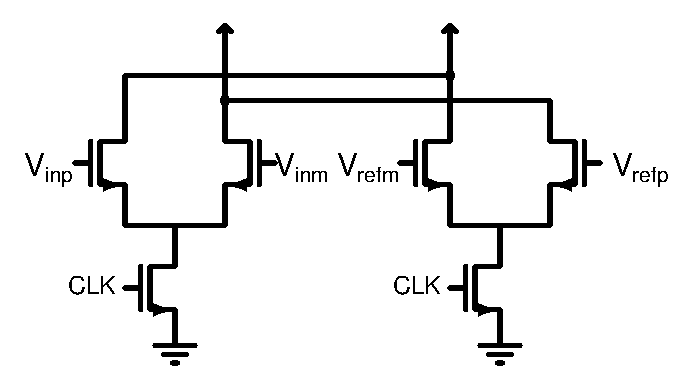
\includegraphics[width=\textwidth]{Chapter7/Figs/sumanen_dblDiffPair}
        \subcaption{Switched Cap~\cite{Sumanen2000}}
        \label{fig:cmp_dbl_diff_sumanen}
    \end{subfigure}
    \begin{subfigure}[b]{0.54\textwidth}
        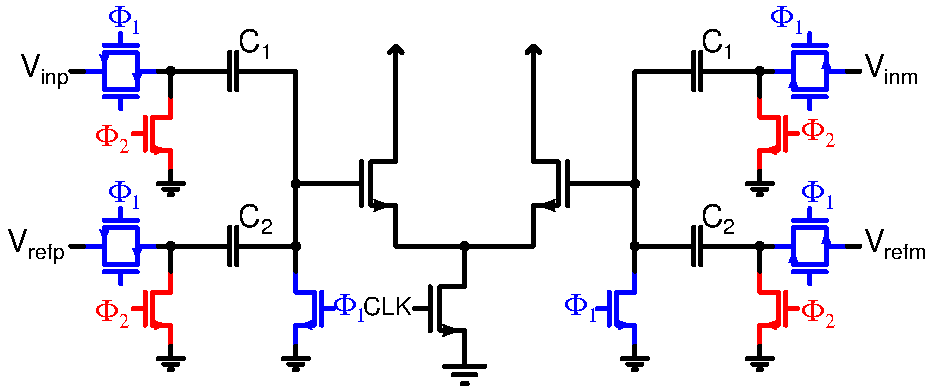
\includegraphics[width=\textwidth]{Chapter7/Figs/sumanen_sc_ref}
        \subcaption{Switched Cap~\cite{Sumanen2002}}
        \label{fig:cmp_sc_diff_sumanen}
    \end{subfigure}
	\caption{Analog subtraction for differential voltage comparison}
	\label{fig:cmp_analog_sub}
\end{figure}

The analog subtraction can be done using two differential pairs as shown in \figurename~\ref{fig:cmp_dbl_diff_sumanen}~\cite{Sumanen2000}. This one-step solution introduces an offset coming from the mismatches between the two input differential pairs. The threshold level is thus fixed by the ratio of differential pair transistors creating a dependence between the offset and the reference voltage applied.

In the charge domain, the subtraction can be implemented as depicted in \figurename~\ref{fig:cmp_sc_diff_sumanen} taken from~\cite{Sumanen2002}. The threshold voltage is now fixed by the capacitor ratio \(C_1/C_2 \) and improves the reference voltage dependence of the offset. Nevertheless, the gain introduced as \(C_1/(C_1+C_2) \) effectively makes the offset and noise of the comparator greater with respect to the input signal. If the comparator offset and noise are limiting constraints, the input signal attenuation caused by the previous architecture may not be tolerable. The circuit to avoid this problem is shown in \figurename~\ref{fig:abo_sc}, and introduced by Abo and Gray in~\cite{Abo1999}. One would rather prefer to change to virtual ground between \(C_2\) capacitors to a proper connection to the ground to enhance reliability.

\begin{figure}[htp]
	\centering
    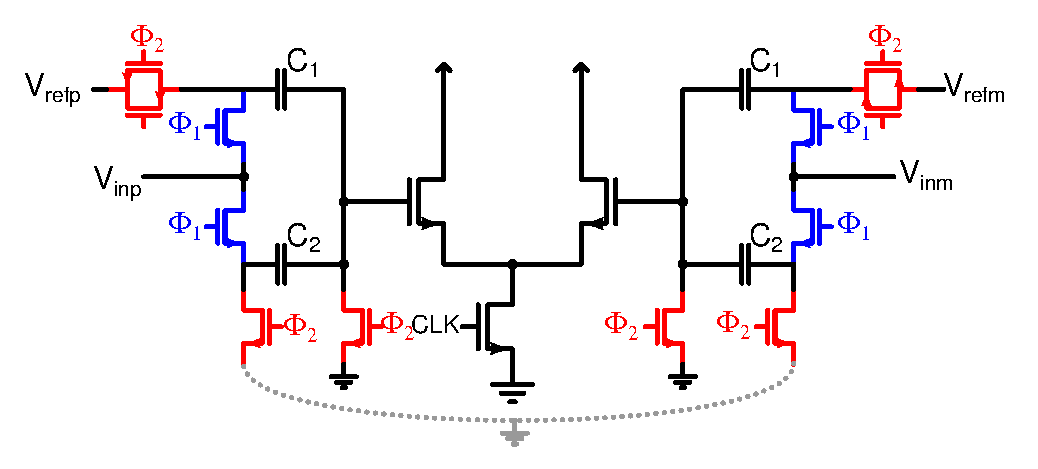
\includegraphics[width=0.75\textwidth]{Chapter7/Figs/abo_sc.ps}
	\caption{Abo implementation of the analog subtraction to prevent voltage compression}
	\label{fig:abo_sc}
\end{figure}

The polarity of the analog subtraction output is then reused by digital logic to perform the conversion. Comparators could be evaluated in different ways, depending on the application. The most generally used figures of merit are probably resolution, followed possibly by delay (speed) and offset. The most important ones from our point of view are listed below:
\begin{multicols}{2}
    \begin{itemize}
        \itemsep-0.5em
        \item[--] Resolution
        \item[--] Delay
        \item[--] Input Referred Offset
        \item[--] Noise
        \item[--] Kickback
        \item[--] Metastability
        \item[--] Power consumption
        \item[--] Hysteresis
    \end{itemize}
\end{multicols}

%\subsubsection{Resolution}
The resolution of a comparator is the minimum difference between the input signals that can be detected. Closely related to the gain of the input stage of a comparator, a comparator is conceptually a high-gain differential amplifier that saturates to the supply rails, or to some other levels. Therefore a high gain amplifier is a first candidate. In the case of closed-loop amplifier that uses positive feedback, the comparison time is involved. The system has two stable points and will follow a trajectory to either one depending on the initial condition. More time is allotted into latching to either state, more sensitive the comparator will be.

%\subsubsection{Delay}
%The delay is the comparison time between the rising (resp. falling) edge of the comparison enable signal (clock) and the instant the output reflect the decision. This delay is the main limiting factor of the analog to digital conversion rate.

%\subsubsection{Input Referred Offset}
%While an ideal comparator detects zero-crossings of the differential input voltage, fabrication mismatches shifts the threshold of detection. This difference is the input referred offset. Therefore, from a comparator to another a given static inputs within the resolution limits outputs different logic value.

%\subsubsection{Noise}
%The former output discrepancy is found between two comparators decision. A real circuits exhibits thermal and other kinds of noise, random fluctuations of quantities (voltages/currents) leading to different outputs for the same static inputs given. An Excessive noise will lead to degraded SNR (ENOB, BER) at system level.

%\subsubsection{Kickback}
%The kickback is a disturbance coming from the comparator to the circuits driving its inputs when a decision is made. This results from a capacitive coupling between a fast changing nodes and the inputs. The repercussions of this fast transient coupling is both differential and common to the inputs. While the differential kickback is undistinguishable from a differential input voltage, the common mode kickback impact is mitigated by the use of a differential architecture.

%\subsubsection{Metastability}
%Metastability is the inability to reach a decision in the available amount of time. It occurs when the input signal is small, or zero. When the differential input voltage is zero the comparator is at the metastable state. Mathematically, the comparator may remain in this state forever. In practice, noise will drive the circuit out of this state. Even so, a small but non-zero input signal will not allow the outputs to reach the switching thresholds in the allotted amount of time.

%\subsubsection{Power consumption}
%The power consumption is the power (often quoted as current) drawn by the comparator in order to perform the comparison. Continuous time and clocked comparator can draw both static and dynamic current.
%Two measures are important: the average current and the maximum peak current drawn. The latter is often neglected in published results, but it is crucial for the layout and decoupling of the voltage supply lines. The average power is usually quoted at a given switching rate.

%\subsubsection{Hysteresis}
%Hysteresis is the property of state-dependent decision threshold. In some cases hysteresis is a desired feature, for example to reject noise superposed on a slowly changing input signal. For our purposes, hysteresis is an undesirable trait that must be avoided. This is commonly done by introducing a reset circuit for every critical internal node.

Open-loop wideband amplifiers have the desirable feature of high initial speed, but suffer from limited resolution and potentially troublesome offset voltage. Latches and positive feedback increase the gain and allow faster decisions. Unfortunately, The first inherent flaw is the rising exponential behavior: the gain is low if the input signal (or the initial condition) is small.
The second drawback is related to the practical realization of a latch. Since the objective is to maximize dynamic gain, one should maximize speed by minimizing capacitance. This is done by using small transistors, which also helps reduce power consumption. However, the mismatch worsens as the devices become smaller, thus fast latches exhibit relatively large input offsets. This drawback hinders the use of latches as comparators for analog to digital conversion.
The best solution is to cascade an open-loop amplifier and a latch. In this way, the overall gain can be distributed over two stages. The first stage has the most dynamic gain near the origin, and outputs a voltage that sets the initial condition of the second stage away from its zero gain region, speeding it up.

\subsubsection{Current Mode Latches}
The earliest comparator circuits using the cascading of a pre-amplifier and a latch were used in current-mode logic (CML) circuits. The first current mode latch was presented by Yamashina et al in a current control logic for processors~\cite{Yamashina1994}. The principle of CML is to use of a differential pair loaded by resistances to amplify the difference between the inputs. The differential output sets the starting voltage of a regenerative amplifier stage. Both stages are biased by constant current sinks, which are switched on and off to reduce the power dissipation. Some examples of CMOS CML can be found in the work of Usama and Kwasniewski~\cite{Usama2004}. The power consumption of CML CMOS comparators can be reduced down to about 182 $\mu$W in a 0.13 µm CMOS technology~\cite{Zhang2014cmp}. These comparators can reach the fastest possible speed, at the expense of large power dissipation. They are typically found in GHz-level serial links where Inter Symbol Interference is a key concern. Nonetheless, they are an example of combining two stages, one linear and one regenerative, to obtain the best performance.

\subsubsection{Single Stage Latches}
Cross-coupled CMOS inverters work as a regenerative amplifier with fully restored logic outputs. Another advantage is that it does not draw any static current and scales well with nanometer technology. The major issue is the offset~\cite{Hajimiri1998}. Several examples can be found in the study released by Stojanovic and Oklobdzija~\cite{Nikolic2000}. With the first use in an ADC by Yukawa and Fujita in 1985~\cite{Yukawa1985} whose offset (one standard deviation) is reported to be less than 3 mV without any offset canceling technique. Nevertheless, it consumes power as long as the input common mode is held in the range where both PMOS and NMOS transistors are conducting. Another impairment is the fact that the memory of the previous state directly influences the comparison threshold as well as both the threshold voltage and the transconductance and the mismatch in the capacitive loads~\cite{Nikoozadeh2006}.

Based on it, comparators found in~\cite{Sumanen2000,Sumanen2002}, and presented earlier for the analog subtraction, are a derivation of a widely used single-stage latched comparator: the Strong-Arm latch.

Introduced by Kobayashi for a memory cell~\cite{Kobayashi1993}, a major reliability issue is floating nodes above the transistors of the differential pair as represented in \figurename~\ref{fig:sa-fn}. The transistor M10 was introduced in~\cite{Montanaro1996} to solve a floating node problem that occurs if the differential input voltage reverses polarity after the decision has been taken. One can also introduce additional reset transistors to remove any memory of previous decisions in all internal nodes as in~\cite{Verbruggen2008}.

\begin{figure}[htp]
    \centering
    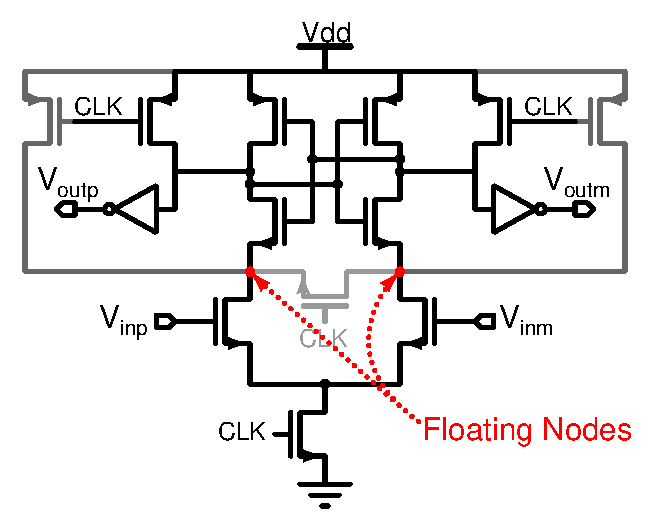
\includegraphics[width=0.3\textwidth]{Chapter7/Figs/StrongArm-FloatingNodes.ps}
    \caption{Floating Nodes of a conventional Strong-Arm latches and method to circumvent from~\cite{Montanaro1996} and~\cite{Verbruggen2008}}
    \label{fig:sa-fn}
\end{figure}

\subsubsection{Two-Stage Latches}
Single stage latched comparators are fast and consume little power. However, they tend to be noisy, to have large offset and kickback noise. To address these problems, a more common practice is to use a pre-amplification stage.
Moreover, at low-voltage operation, the 4-transistor stack of a StrongArm latch reduces the headroom of the input pair transistors.

In 2006, Chen and Brodersen added reset switches in both the pre-amplifier and latch stage to reduce the comparator recovery time during the reset phase~\cite{Brodersen2006}. Reset transistors of the pre-amplifier are also used for input offset cancellation technique. In addition, the current mirror between the two stages is useful to reduce charge kickback from the logic level swing of the latch~\cite{Bult1997}. This technique decreases the offset and the hysteresis. Proposed in a SAR ADC realized in 0.13 \(\mu\)m, the 6-bit ADC performs at 600MS/s~\cite{Brodersen2006} while the analog core consumes 1.2 mW. Yet, the current consumption is more important than CML latch since a large transient current runs through the latch at the beginning of a decision while the pre-amplifier consumes a static current over the full clock period.

\begin{figure}[htp]
	\centering
	\begin{subfigure}[b]{0.32\textwidth}
        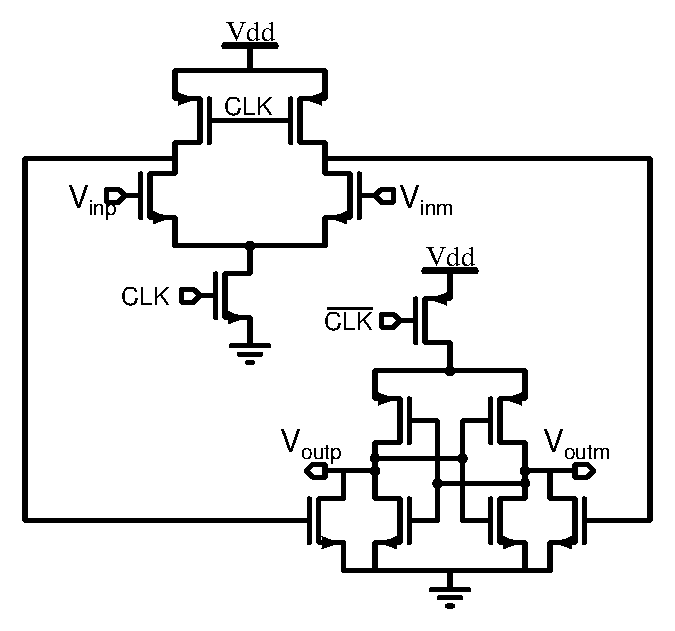
\includegraphics[height=4cm]{Chapter7/Figs/dbl_tail_schinkel.ps}
        \subcaption{Schinkel~\cite{Schinkel2007,Savani2015}}
        \label{fig:dbl_tail_shinkel}
    \end{subfigure}
    \begin{subfigure}[b]{0.32\textwidth}
        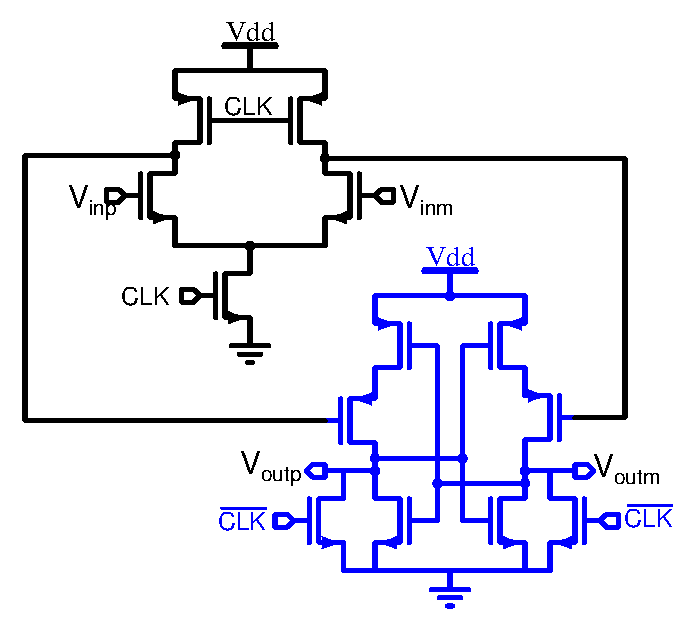
\includegraphics[height=4cm]{Chapter7/Figs/dbl_tail_elzakker.ps}
        \subcaption{Van Elzakker~\cite{Elzakker2010}}
        \label{fig:dbl_tail_elzakker}
    \end{subfigure}
    \begin{subfigure}[b]{0.32\textwidth}
        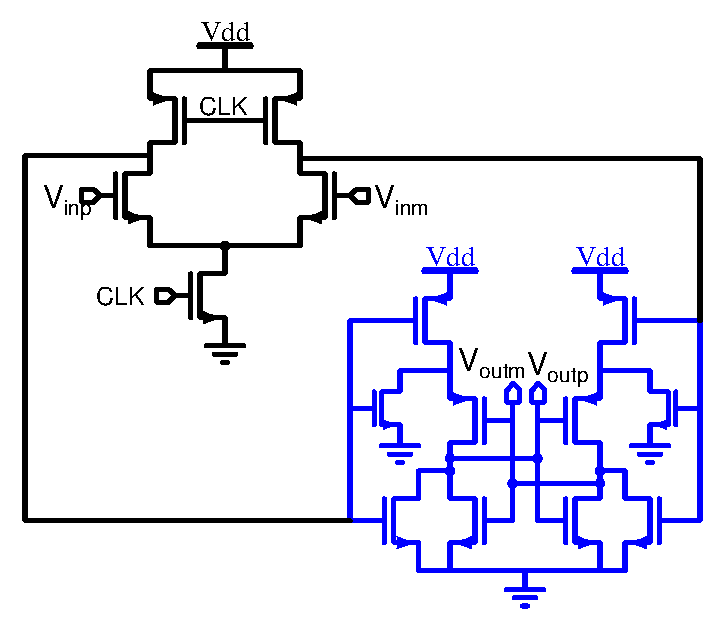
\includegraphics[height=4cm]{Chapter7/Figs/dbl_tail_miyahara.ps}
        \subcaption{Miyahara and Asada~\cite{Miyahara2008}}
        \label{fig:dbl_tail_miyahara}
    \end{subfigure}
    \begin{subfigure}[b]{0.48\textwidth}
        \centering
        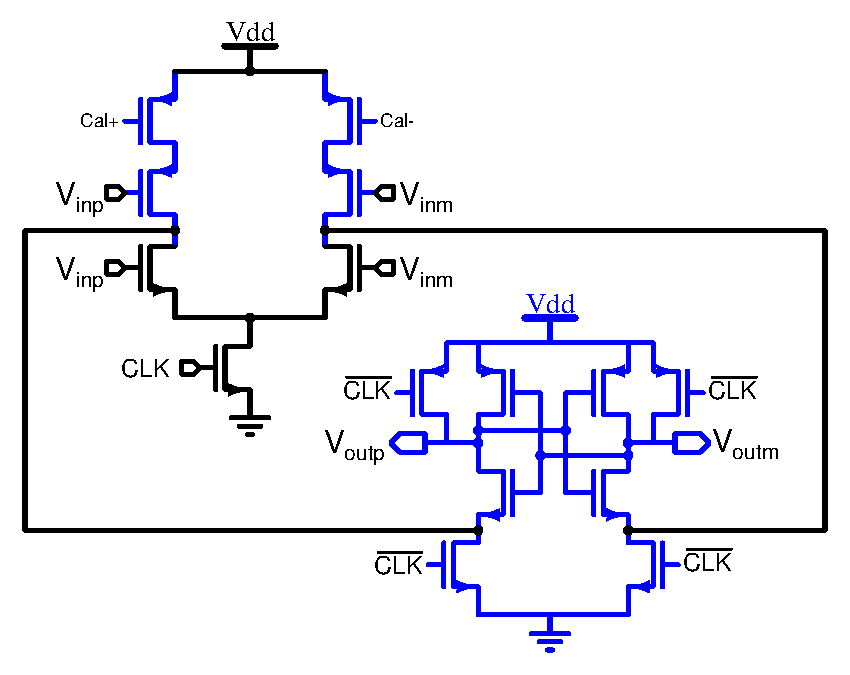
\includegraphics[height=4cm]{Chapter7/Figs/dbl_tail_chan.ps}
        \subcaption{Chan et al.~\cite{Chan2011}}
        \label{fig:dbl_tail_chan}
    \end{subfigure}
    \begin{subfigure}[b]{0.48\textwidth}
        \centering
        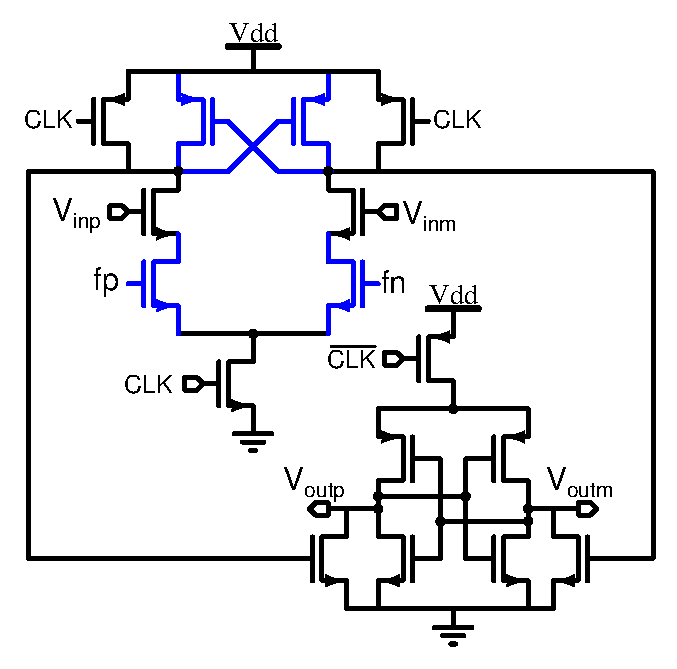
\includegraphics[height=4cm]{Chapter7/Figs/dbl_tail_babayan.ps}
        \subcaption{Babayan-Mashhadi~\cite{Babayan2014}}
        \label{fig:dbl_tail_babayan}
    \end{subfigure}
    %\begin{subfigure}[b]{0.48\textwidth}
    %    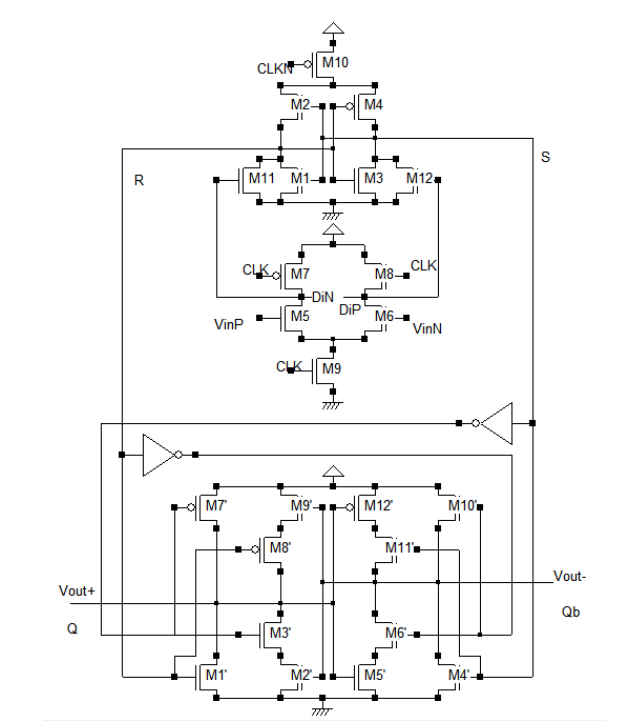
\includegraphics[height=4cm]{Chapter7/Figs/dbl_tail_savani.png}
    %    \subcaption{Savani~\cite{Savani2015}}
    %    \label{fig:dbl_tail_savani}
    %\end{subfigure}
	\caption{Usual variations of the double tail comparator over its original version}
	\label{fig:dbl_tail_comp}
\end{figure}

To be energy-efficient a comparator can also have a pre-amplifier that is efficient too. Van Elzakker bases his comparator on a recent structure introduced by Schinkel~\cite{Schinkel2007, Elzakker2010}. Compared to the previous architecture, the double tail has less stacked transistors in order to operate even at very low voltage. \figurename~\ref{fig:dbl_tail_comp} represents the different variations around the double tail architecture. The main change noticed is the choice of the second stage. The speed can be further increased by the introduction of a positive feedback inside the pre-amplifier as in~\cite{Bult1997,Babayan2014} at the price of an extra kickback. The dynamic pre-amplification proves to be as efficient as in~\cite{Savani2015} with a supply voltage of 1 V and a clock at 1 GHz, the estimated power consumption is around 17 \(\mu \)W.

An overall comparison of comparators is presented in \tablename~\ref{table:comp_comparison_table}.

\begin{table}[htp]
	\caption{Comparators Performances}
	\centering
	\label{table:comp_comparison_table}
	\begin{tabular}{L{4.5\charwidth} R{10\charwidth} R{4\charwidth} R{10\charwidth} R{5.5\charwidth} R{5.5\charwidth} R{6\charwidth} R{5.5\charwidth} C{8.5\charwidth}}
	\toprule
	Ref. & Architecture & \multicolumn{2}{c}{Technology [nm]}  & Delay [ps] & {\makecell{{\(\sigma_{Offset} \)} \\ {[mV]}}} & Supply [V] & Power [\(\mu \)W] & Res./Load [mV/pF] \\
    \midrule
	\cite{Sumanen2000}    & Strong Arm  & 500  & Bulk CMOS & <5000 & 10 & 3   &  837 & NC/20\\
    \cite{Yamashina1994}  & CML         &  NA  & Bulk CMOS & 200   & NA & 1.2 & 1000 & 200/NC\\
	\cite{Usama2004}      & CML         & 180  & Bulk CMOS & 112   & NA & 1.2 &  275 & 1200/2\\
	\cite{Zhang2014cmp}   & CML         & 130  & Bulk CMOS &  66   & NA & 1.2 &  182 & 1200/NC\\
	\cite{Nikolic2000}    & Strong Arm  & 180  & Bulk CMOS & 175   & NA & 1.8 &   31 & 1800/0.2\\
	\cite{Yukawa1985}     & Two-Stage   & 1200 & Bulk CMOS & 7000  & 2  & NA  & 1300 & 10/NC\\
    \cite{Verbruggen2008} & Strong Arm  &  90  & Bulk CMOS & <570  & 27 & 1   &   32 & 25/NC\\
	\cite{Schinkel2007}   & Double Tail &  90  & Bulk CMOS &  165  & 9  & 1.2 &  225 & 10/NC\\
    \cite{Savani2015}     & Double Tail &  90  & Bulk CMOS &  142  & NA & 1   &   17 & 1000/NC\\
    \cite{Elzakker2010}   & Double Tail &  65  & Bulk CMOS & 1300  & NA & 1   & 0.06 & 2/NC\\
    \cite{Miyahara2008}   & Double Tail &  90  & Bulk CMOS &  122  & 13 & 1   &   40 & 1/NC\\
    \cite{Babayan2014}    & Double Tail & 180  & Bulk CMOS & 800   &  8 & 0.8 &  576 & 5/NC\\
	\bottomrule
	\end{tabular}
\end{table}
\nomenclature{$\sigma_i$}{standard deviation of $i$}

\clearpage
    \subsection{Amplifiers}                      % section 4.1.3
\label{sec:amplifier-review}
Switched capacitor analog is proven first-class candidate for critical analog function implementation in mixed-signal systems. Fully compatible with modern digital cmos they required amplifiers, capacitors, and clocked switches.

Amplifiers' role in the high-accuracy systems is twofold: either in delta charge flow or in charge transfer implementation the amplifier preserves the charge stored on a capacitor and maintains the signal, and in a charge transfer implementation they also are responsible for moving charges from one capacitor into another.

\begin{figure}[htp]
    \centering
    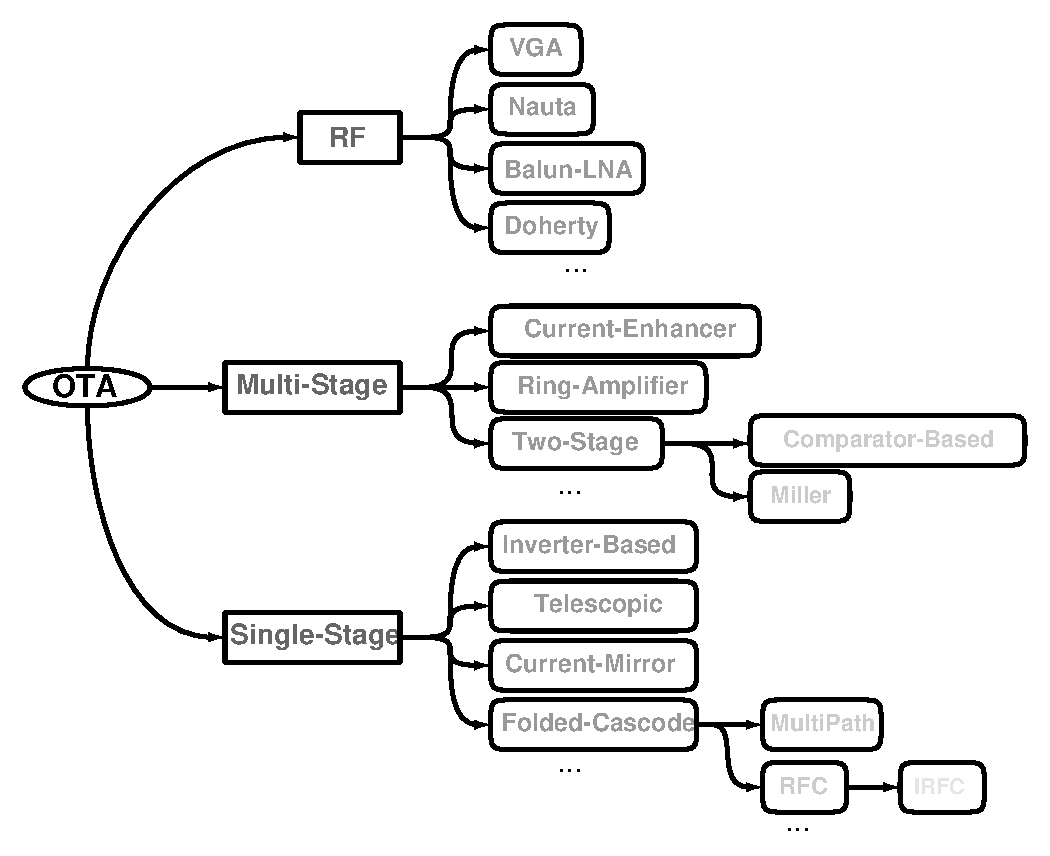
\includegraphics[width=0.75\textwidth]{Chapter7/Figs/family_amplifier.ps}
    \caption{Family tree of common amplifiers architecture}
    \label{fig:ota_tree}
\end{figure}

Depending on the applications many amplifier topologies have emerged. A non-exhaustive list of common topologies is, in Figure~\ref{fig:ota_tree}, grouped into three categories: RF, Single Stage, and MultiStage.

Focused on a high gain and high-speed amplifiers, all amplifiers for RF communications are not suited for the conception of an ADC\@. Indeed, they reach with difficulty 20 dB of DC Gain and are power hungry~\cite{Nauta1992, Chen2014}.

The analog design insight over temperature in Section~\ref{sec:analog-insight} highlight the difficulty to achieve a stable high-gain over temperature and a high-speed amplifier based on a single transistor performance. Therefore, high-gain amplifiers usually use either cascode and multi-stage architectures~\cite{Bult1990}. In a multi-stage amplifier, each stage contributes in its simplest form as an extra pole and an extra zero. In this regard, to ensure the Barkhausen stability criterion, phase compensation schemes are required to obtain a good phase margin.
To the contrary, high bandwidth amplifiers use a single-stage architecture, high bias current, and short channel devices.

Among single stage amplifiers, inverter-based amplifiers are often used in ADC and well-reputed for their low-power consumption~\cite{Selby2013,Ismail2016}. Nevertheless, limited bandwidth and the biasing of transistors based on the change of the supply voltage are not suited for a high-speed ADC in an automotive environment.
%According to [10], the Current Mirror Cascode OTA has a high GBW and slew rate with a fast settling time. Nevertheless, those amplifiers have a non-dominant pole at the input of its current-mirror. Due to this additional pole the phase margin is limited and depends of the current mirror ratio.
%Those amplifiers efficiency can be greatly improved by using current shunt, current reuse, or current shunt with a positive feedback [11]. Those techniques improve the gain, the output resistance, and noise performances. The compromise is the parasitic effect induced by extra transistors penalizing the phase margin already low. Therefore, the current mirror OTA is not recommended in the design of a stable amplifier across process variations.
To reduce the power consumption of amplifiers and reduce analog design constraint, the one could implement a continuous-time comparator with a push-pull stage as a comparator based ADC\@. This has been discussed in~\cite{Fiorenza2006}, to build an 10-bits pipelined ADC whose power consumption is 2.5 mW at 7.9 MSamples/s in 0.18 \(\mu \)m CMOS technology. Nevertheless, this comes at a cost of an increased complexity in the digital switching more sensitive to jitter.

\begin{figure}[htp]
    \centering
    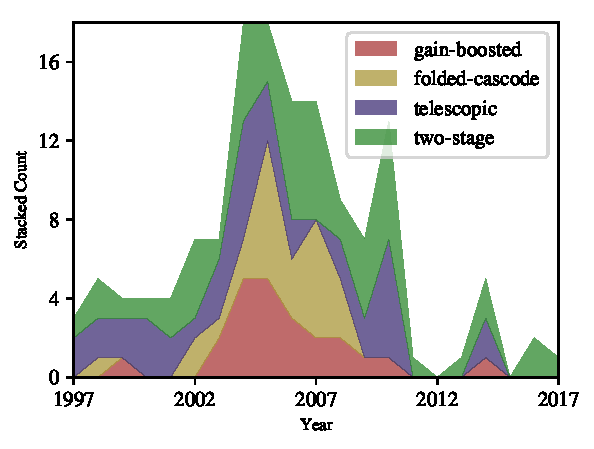
\includegraphics[width=0.75\textwidth]{Chapter7/Figs/amplifier_repartition.pdf}
    \caption{Repartition for \(\Delta\Sigma \) and Pipelined over Years 1997-2017 of ISSCC and VLSI ADCs in \cite{MurmannSurvey}}
    \label{fig:ota_over_year}
\end{figure}

Figure~\ref{fig:ota_over_year} represents the repartition over years of usual topologies for technology over 65 nm. For the sake of clarity, only four topologies have been selected. Furthermore, for a given year, the results are stacked such that the total number of publications and the number of publications using one topology is represented.
For the 0.18 \(\mu \)m CMOS process, most of the publications have been published between 2001 and 2008. Over this period, the Folded-Cascode (FC), Two-Stage (TS), and Gain-Boosting (GB) were mainstream with a large preference for folded cascode amplifier either alone or followed by a source follower stage to enlarge the output swing.

Traditionally, folded-cascode OTA has been preferred for high-speed switched capacitor applications~\cite{Olivera1999, Adut2003} because of their high DC gain and GBW\@. This architecture candidate is proven to operate under low voltage conditions, even for larger process node size: down to 0.7 V~\cite{Sauerbrey2002, Ahn2005}.
\nomenclature[z]{GBW}{Gain-BandWidth product}
\nomenclature[z]{UGF}{Unity-Gain-Frequency}
The Telescopic OTA (Tele.) provides better current efficiency, hence consumes less power, but suffers from limited output swing~\cite{Quinn2000}. Such a limitation is circumvented by the use of pseudo-differential architecture as in~\cite{Chiu2004}.

The Table~\ref{table:ota_comparison_table} lists some amplifiers used in ADC between 12-bits and 14-bits of resolution.

\begin{table}[htp]
	\caption{OTA Performances}
	\centering
	\label{table:ota_comparison_table}
	\begin{tabular}{L{5\charwidth} L{4.2\charwidth} L{11\charwidth} R{4.5\charwidth} R{4.5\charwidth} R{3.5\charwidth} R{4.5\charwidth} C{9\charwidth} C{6.2\charwidth} C{5.5\charwidth}}
	\toprule
	Ref. & Tech. [\(\mu \)m] & Topology & Gain [dB] & UGF [MHz] & PM [\(\degree \)] & Load [pF] & Out Swing [V] & Supply [V] & Power [mW] \\
    \midrule
    \cite{Sauerbrey2002}  & 0.18 & TS (FC+SF\footnotemark[1]) & 50  &   10 & 80 & 4    & 0.5 & 0.7 & 0.055 \\
    \cite{Chiu2004}       & 0.18 & Pseudo-Diff Tele. GB       & 130 &   NA & 70 &   NA & 2\footnotemark[2] & 1.8 & 16 \\
    \cite{Bult1991}       &  1.6 & FC GB                      & 90  &  116 & 64 & 16   & 4.2 & 5 & 52 \\
    \cite{Miyahara2014}   & 0.18 & TS                         & 88  &  250 & NA &   NA & 2\footnotemark[2] & 1.6 & 27.4 \\
    \cite{Thandri2006}    & 0.35 & TS                         & 80  & 1400 & 62 &  2   & NA & \(\pm \)1.25 & 11.5 \\
    \cite{Zhang2015PRIME} & 0.13 & FC GB                      & 85  & 4750 & 50 &  1.6 & 1.2 & 1.5 & NA \\
    \cite{Liu2015OpAmp}   & 0.18 & Tele. GB                   & 102 & 1200 & NA & 0.48 & NA  & 1.8 & 1.7 \\
    \cite{Sun2016}        & 0.18 & Buffered TS                & 81  & 1500 & 68 &  0.5 & NA  & 1.9 & 22.8 \\
	\bottomrule
	\end{tabular}
\end{table}
\footnotetext[1]{folded cascode amplifier followed by a source-follower}
\footnotetext[2]{Volt peak-peak}

For a 0.18-$\mu m$ technology, the Folded Cascode OTA with Gain Boosting or a Telescopic OTA with gain boosting are the best candidates. In order to cope with 10\% power supply variations and a large output swing needed, the Folded Cascode OTA with Gain Boosting is preferred.
The advantage of this solution is a reduced area overhead compared to a two-stage implementation with a greater bandwidth achievable.

Before diving into the design of a complex OTA over temperature, let us start with simpler circuits: the comparators.

\clearpage
\section{Latch comparator design}                       % section 4.2
\label{sec:comp-delay-design}
    \subsection{Use case}                     % section 4.2.1
The hybrid pipelined architecture contains an I\(\Delta\Sigma \) stage followed by an algorithmic stage and a SAR stage. In principle, all stages share the same common-mode and reference voltage levels. In addition, the proposed hybrid converter should operate from -40\(\degree \)C up to +175\(\degree \)C. Each one of these stages imposes different constraints on the amplifier and the comparators within.

As a trade-off between output swing, linearity, and gain at a given speed to realize the ADC, some constraints can be relaxed by implementing at least a 1.5-bit encoder for the first two stages. From the review done in Section~\ref{sec:latches}, a switched capacitor analog subtraction is preferred in this regard for the reduced temperature variation of the capacitor over the current variation of the double differential pair variation.

The incremental and the algorithmic stages are closed-loop converters. Therefore, the only effect of errors introduced by the comparators is to increase the amplitude of the residue passed on to the following stage. Those two first stages are fault tolerant while the comparator errors do not exceed a rather relaxed level of non-correctable error.

From a design point of view, both the strong arm and the double tail comparator do not keep the result from a clock period to another. Therefore, they are followed by an RS-latch in charge of keeping the decision made for the digital circuits. This RS-latch is thus the load seen by the comparator.

    \subsection{Strong Arm Latch vs Double Tail} % section 4.2.2
\begin{figure}[htp]
    \centering
    \begin{subfigure}[b]{0.36\textwidth}
        \centering
        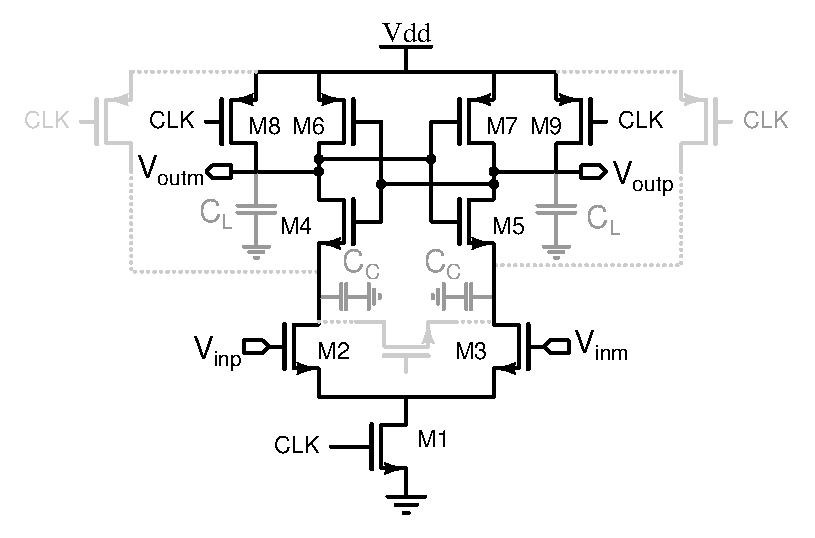
\includegraphics[width=\textwidth]{Chapter7/Figs/sa_designed.eps}
        \subcaption{Strong-Arm}
        \label{fig:sa_designed}
    \end{subfigure}
    \begin{subfigure}[b]{0.62\textwidth}
        \centering
        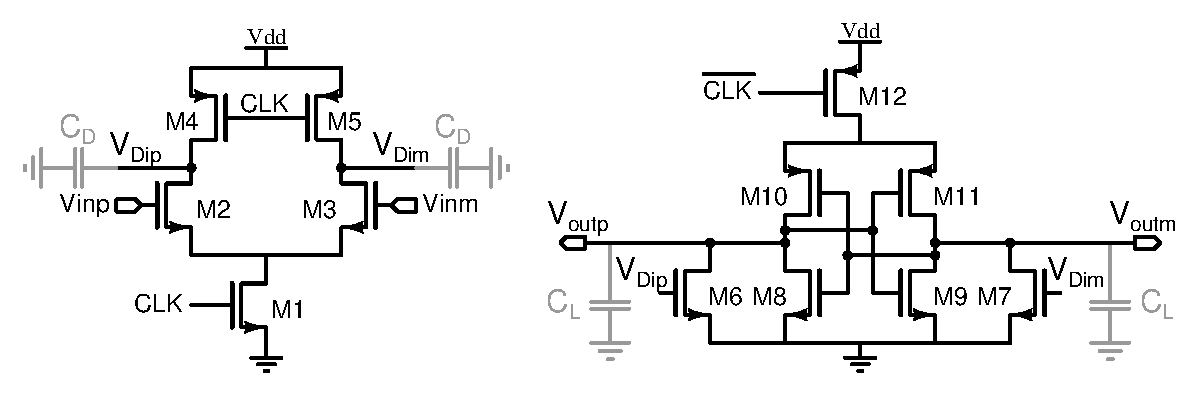
\includegraphics[width=\textwidth]{Chapter7/Figs/dtl_designed.eps}
        \subcaption{Double Tail}
        \label{fig:dtl_designed}
    \end{subfigure}
    \caption{Comparators designed for the temperature}
    \label{fig:cmp_designed}
\end{figure}

The Strong ARM (SA) latch depicted by \figurename\ref{fig:sa_designed} has been chosen for its rail-to-rail output and a quite fast response with small power consumption. The Double-Tail architecture is a promising candidate for low-power, reduced voltage, and scaling.
\subsubsection{Delay}
The detailed operation of the SA latch has been studied thoroughly~\cite{Wicht2004, Razavi2015}.
In a nutshell, the reset state (CLK=0 V) sets the transistors M4-M5 that are in a deep sub-threshold region, and the outputs are pulled up to \(V_{DD}\) by M8-M9. No current flows in the differential pair because M1 is also off.
Once the clock is active (CLK=\(V_{DD}\)), M1 turns on hard in the linear region, and M2-M3 convert the differential input voltage \(\Delta V_{in}\) into a current that pulls down the voltages at the sources of NMOS devices M4-M5 until they start to conduct.
Once \(V_{outm}\) or \(V_{outp}\) reach \(V_{DD}-V_{thp}\), M6-M7 turn on and the cross-coupled inverters regenerates the voltage imbalance \(\Delta V_{out}(t_{lin}) = V_{outp}(t_{lin}) - V_{outm}(t_{lin})\). In order to derive \(t_{lin}\), we will assume that the discharge rate is constant as well as \(C_{C}\) and \(C_{L}\): the total capacitance loads at the sources of M4-M5 and the total capacitance load at the output nodes.

\begin{eqnarray}
\label{eq:sa_tout_lin}
t_{lin} = V_{thp}\frac{{C_{L}+C_C}}{I_{M2,M3}}   \\
\Delta V_{out}(t_{lin}) = \frac{I_{M3}-I_{M2}}{{C_{L}+C_C}}t_{lin}  \label{eq:sa_dout_lin}
\end{eqnarray}

The regeneration to fully restored logic values (\(V_{logic}\)) denoted by \(t_{reg}\)is given by equation~(\ref{eqn:sa_tout_reg}). The total propagation delay of the comparator is then the sum of \(t_{lin}\) and \(t_{reg}\).
\begin{equation}
    \label{eqn:sa_tout_reg}
t_{reg} = \frac{C_{L}}{g_{m4,m5}+g_{m6,m7}} \ln{\left(\frac{V_{logic}}{\Delta V_{out}(t_{lin})}\right)}
\end{equation}

To reach the maximum speed, transistors in the differential pair and of the current source are biased in strong inversion according to \figurename~\ref{fig:tradeoffs}. With a quadratic model leading to the approximate \(g_m/I_d \approx 2/V_{ov}(T)\), the variation of the delay with respect to the temperature can be found to be
\begin{equation}
\label{eqn:sa_dt_dT}
\frac{1}{t_{lin}}\frac{\partial t_{lin}}{\partial T} = (C_L+C_c) \left[ \alpha_{vthp} \left(\frac{g_{m2,m3}}{I_{d2,d3}}(T) - \frac{1}{V_{thp}(T)} \right) + \alpha_\mu \left(\frac{T_0}{T} \right) \right]
%\frac{\mu_0 C_{ox} W}{2 L C_L} \frac{\partial t_{lin}}{\partial T}= \frac{1}{4}{\left(\frac{g_m}{I_d}(T)\right)}^2 \left[\alpha_{V_{th}}{\left(\frac{T}{T_0} \right)}^{-\alpha_\mu}\left(1+\frac{g_m}{I_d}(T) \right)\left(1-\frac{\alpha_\mu}{\alpha_{V_{th}}}\frac{T}{T_0} \right)V_{th}(T) \right]
\end{equation}

The variation of time spent in the linear phase is thus minimized for a small \(g_m/I_d\) and a low-\(V_{th}\) transistor. And the delay unconditionally increases in this architecture with the temperature.

Among methods to prevent the floating drain of the differential pair transistor, the solution presented in~\cite{Montanaro1996} also affects the speed of the decision as demonstrated in Appendix~\ref{appx:latch_models}.

In comparison, the double tail (DT) comparator~\cite{Schinkel2007}, shown in Figure~\ref{fig:dtl_designed}, is becoming a popular alternative to the SA comparator in the past few years, together with its variations~\cite{Miyahara2008,Babayan2014,Khorami2016}. The key idea is to split the pre-amplification from the latch to decouple the constraints, and to increase the voltage headroom. This section develops an original model for the propagation delay taking into account the current drawn by transistors M6-M7 to improve the accuracy of the previously attempted model~\cite{Babayan2014}.

Briefly, during the reset phase (CLK=0V), the tail transistor M1 is off and transistors M4-M5 are on. The drains of M2-M3 are pulled up to \(V_{DD}\) which discharge to the ground the output nodes of the cross-coupled latch thanks to M6-M7. This is possible because M12 is driven by a complementary clock signal.
Once the clock toggles to \(V_{DD}\), M4-M5 turn off, M1 turns on and the differential pair M2-M3 discharges the internal nodes \(V_{Dip}\) and \(V_{Dim}\) to the ground, at slightly different rates: \(I_{M2,3}/(2C_{D})\). Transistor M12 turned on and \(V_{Dip}\) and \(V_{Dim}\) translated by M6-M7 into a current imbalance at the output nodes, the output voltages are ramping up at a rate of \((I_{M12}/2-I_{M6,M7})/C_{L}\). This until the drain voltage of M8-M9 has risen \(V_{thn}\) above ground, when one can consider that regeneration takes over and the currents drawn by M6-M7 no longer matter.

\(t_{lin}\) is deduced by the equation~(\ref{eqn:dtl_tout_lin})

\begin{equation}
\label{eqn:dtl_tout_lin}
t_{lin} = \frac{C_D}{2C_L} \left(\frac{g_{m6,m7}V_{DD}-I_{M10,M11}}{g_{m6,m7}I_{M2,M3}} + \frac{C_L\sqrt{\xi}}{g_{m6,m7}I_{M2,M3}} \right)
\end{equation}
where
\begin{equation}
\xi = {\left(g_{m6,m7}V_{DD}-I_{M10,M11}\right)}^2  + 4V_{thn}\frac{g_{m6,m7}I_{M2,M3}(C_{L})}{C_D}
\end{equation}
and \(\Delta V_{out}(t_{lin})\) is given by equation~(\ref{eqn:dtl_dout_lin})
\begin{equation}
\label{eqn:dtl_dout_lin}
\Delta V_{out}(t_{lin}) = V_{op}-V_{om} \approx \frac{g_{m6}I_{M2}-g_{m7}I_{M3}}{(C_{L})C_D}t_{lin}^2
\end{equation}

Similarly to the Strong Arm latch, the regeneration time is given by equation~(\ref{eqn:dtl_tout_reg}), and the total delay as the sum of (\ref{eqn:dtl_tout_lin}) + (\ref{eqn:dtl_tout_reg}).

\begin{equation}
\label{eqn:dtl_tout_reg}
t_{reg} = \frac{C_{L}}{g_{m10,m11}+g_{m8,m9}} \ln{\left(\frac{V_{logic}}{\Delta V_{out}(t_{lin})}\right)}
\end{equation}

The minimization of temperature variation of the delay comes by the minimization of the value \(4V_{thn}\frac{C_L^3}{g_{m6,m7}I_{M2,M3}(C_{D})}\) and the minimization of the thermal dependence of \(\frac{g_{m6,m7}V_{DD}-I_{M10,M11}}{g_{m6,m7}I_{M2,M3}}\). The latter can be minimized for low \(\frac{g_m}{I_d}\) of the differential pair transistor and a large voltage overdrive of transistor M6, M7.

\subsubsection{Input Referred Offset}
\begin{figure}[htp]
    \centering
    \begin{subfigure}[b]{0.44\textwidth}
        \centering
        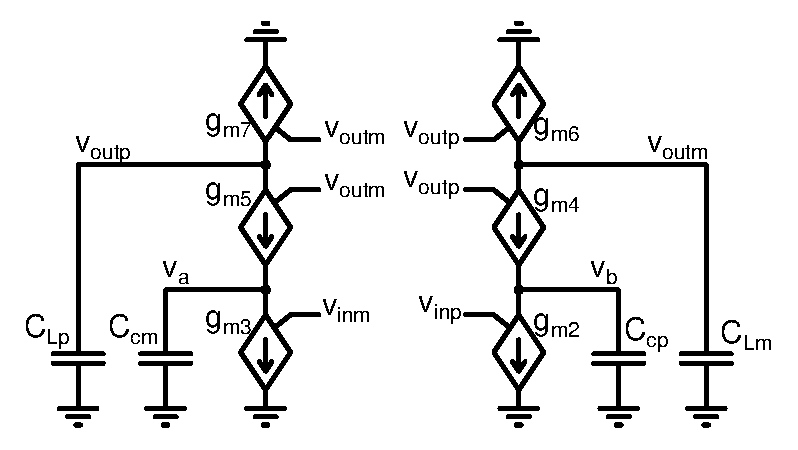
\includegraphics[width=\textwidth]{Chapter7/Figs/sa_small_signal_model.ps}
        \subcaption{strong arm}
        \label{fig:sa_small_signal}
    \end{subfigure}
    \begin{subfigure}[b]{0.54\textwidth}
        \centering
        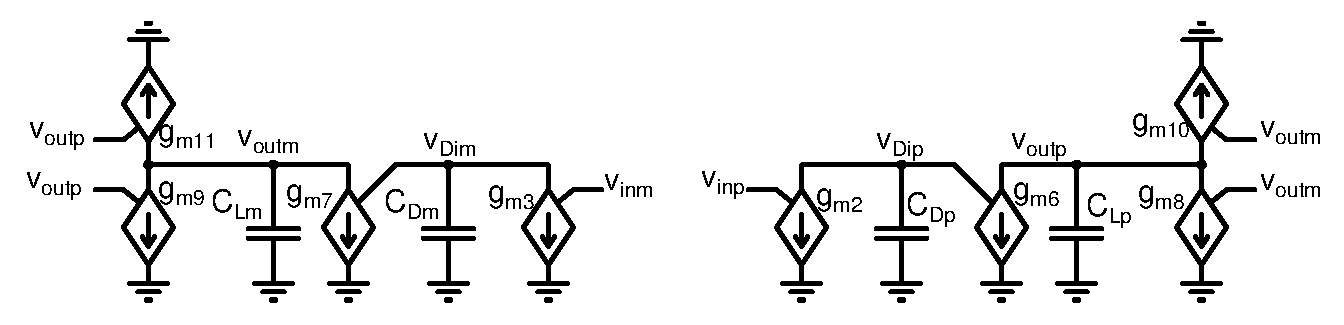
\includegraphics[width=\textwidth]{Chapter7/Figs/dtl_small_signal_model.ps}
        \subcaption{double tail}
        \label{fig:dt_small_signal}
    \end{subfigure}
    \caption{Latches Small Signal Models}
    \label{fig:latches_small_signal}
\end{figure}

As explained by Razavi for the Strong-Arm Latch in~\cite{Razavi2015}, the dominant contributor to the offset, are the transistors in the differential pair. Exploiting the small-signal model represented in \figurename~\ref{fig:sa_small_signal}, the input referred offset is given by equation~(\ref{eqn:offset_sa}).

\begin{align}
    \label{eqn:offset_sa}
    \frac{v_{offset}}{2} \left( \frac{g_{m3}}{1+s\frac{C_{cm}}{g_{m5}}} + \frac{g_{m2}}{1+s\frac{C_{cp}}{g_{m4}}} \right) &= \left( g_{m4}+g_{m6}-g_{m5}-g_{m7}-s\left(C_{Lp}-C_{Lm}\right) \right) v_{outc} \\
    &+ v_{outc} \left( \frac{g_{m5}}{1+s\frac{C_{cm}}{g_{m5}}} - \frac{g_{m4}}{1+s\frac{C_{cp}}{g_{m4}}} \right) \nonumber \\
    &+ v_{inc} \left( \frac{g_{m3}}{1+s\frac{C_{cm}}{g_{m5}}} - \frac{g_{m2}}{1+s\frac{C_{cp}}{g_{m4}}} \right) \nonumber
\end{align}

The equation~(\ref{eqn:offset_sa}) fits the explanation given by both~\cite{Razavi2015} and~\cite{Abidi2014}: the output capacitance contributes to the dynamic offset. Both expect a small mismatch for large capacitors due to the proportion of the error committed by a non-ideal manufacturing process over the size of the capacitance. For small capacitance at the output, the offset is greater. In addition, both the input and output common mode voltage have an impact on the offset. The input common mode voltage (\(V_{inc}\)) in our converter is already set. And the higher the output common mode voltage (\(V_{outc}\)) is, the higher the offset will be.

By the way, the small signal model of the DT latch results in the approximation of~(\ref{eqn:offset_dtl}). The offset originates from the mismatch, in the same manner, it is in the SA latch: a dynamic offset and a static one.

\begin{align}
\label{eqn:offset_dtl}
-\frac{V_{offset}}{2} \approx & V_{outc}\frac{\left[s \left(C_{L1} - C_{L2}\right) + \left(g_{m1}+g_{m2}\right) -\left(g_{m3}+g_{m4}\right)\right] s \left(C_{g5} + C_{g6}\right)}{2(g_{m11}+g_{m10})}\\
+ & V_c \frac{\left[s \left(C_{g5}-C_{g6}\right) + \left(g_{m5}-g_{m6}\right)\right]}{g_{m11}+g_{m10}}  \nonumber  \\
+ & V_{inc}\frac{g_{m11}-g_{m10}}{g_{m11}+g_{m10}} \nonumber
\end{align}

The DT offset abide the input/output common mode alteration, and with the mismatch of parasitics. Thus, both outputs shall be connected to almost similar cells. An RS-latch fits this purpose as it also keeps the decision made once the comparator is reset.

    \subsection{Simulation Results}              % section 4.2.2
\label{sec:latches_sim}
In order to check specific parameters of the comparators designed, a test bench has been set-up to extract the delay, the offset, the hysteresis, the kickback and the power consumption. The test bench represented in \figurename~\ref{fig:cmp_testbench} consists in the generation of a triangle stepped differential input voltage. The output of the RS-latch is thus a window whose edges correspond to the offsets and their difference is the hysteresis. The time span between the clock rising edge and an edge of this window coincide with the delay of the comparator and of the RS-latch.

\begin{figure}[htp]
    \centering
    \begin{subfigure}[b]{0.40\textwidth}
        \centering
        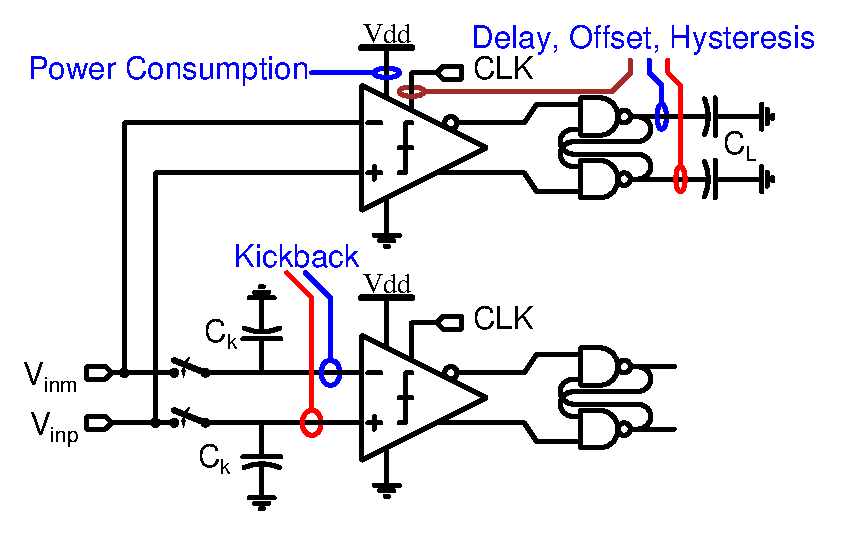
\includegraphics[width=\textwidth]{Chapter7/Figs/cmp_tb.ps}
        \subcaption{schematic}
        \label{fig:cmp_tb}
    \end{subfigure}
    \begin{subfigure}[b]{0.58\textwidth}
        \centering
        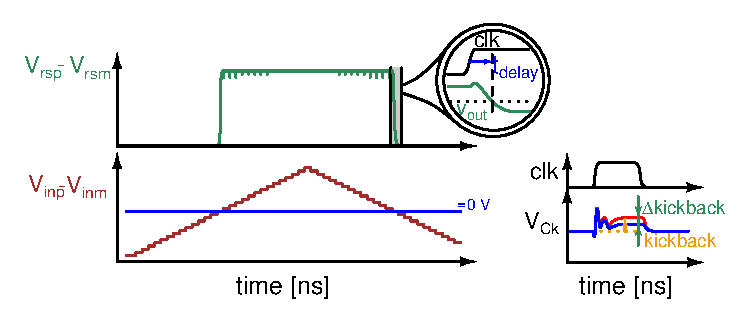
\includegraphics[width=\textwidth]{Chapter7/Figs/cmp_tb_signals.ps}
        \subcaption{test signals}
        \label{fig:test_signals}
    \end{subfigure}
    \caption{Extraction comparators characteristic in spice simulation for fast Monte-Carlo Analysis of simulations}
    \label{fig:cmp_testbench}
\end{figure}

To extract the common mode and the differential kickback, capacitors on the inputs (\(C_{k}\)) are connected to the desired input voltages while the comparator is reset (CLK=0 V). When the clock triggers the comparator, switches are already open. The voltage across \(C_{k}\) is sampled before the reset.

Thus, the error between the ideal input voltage and the sampled voltages gives us the kickback of the comparator for a capacitive load \(C_{k}\). As the comparator is used in a fully differential architecture, the common-mode kickback has less importance than the differential kickback has.

A Strong-Arm and a Schinkel-Double-Tail have been designed for the same offset standard deviation. Once laid out as in \figurename~\ref{fig:layout-comp}, and parasitic extracted, a 100 point Monte-Carlo analysis of their characteristic inside the test bench is performed.

\begin{figure}[!htp]
    \centering
    \begin{subfigure}[b]{0.48\textwidth}
        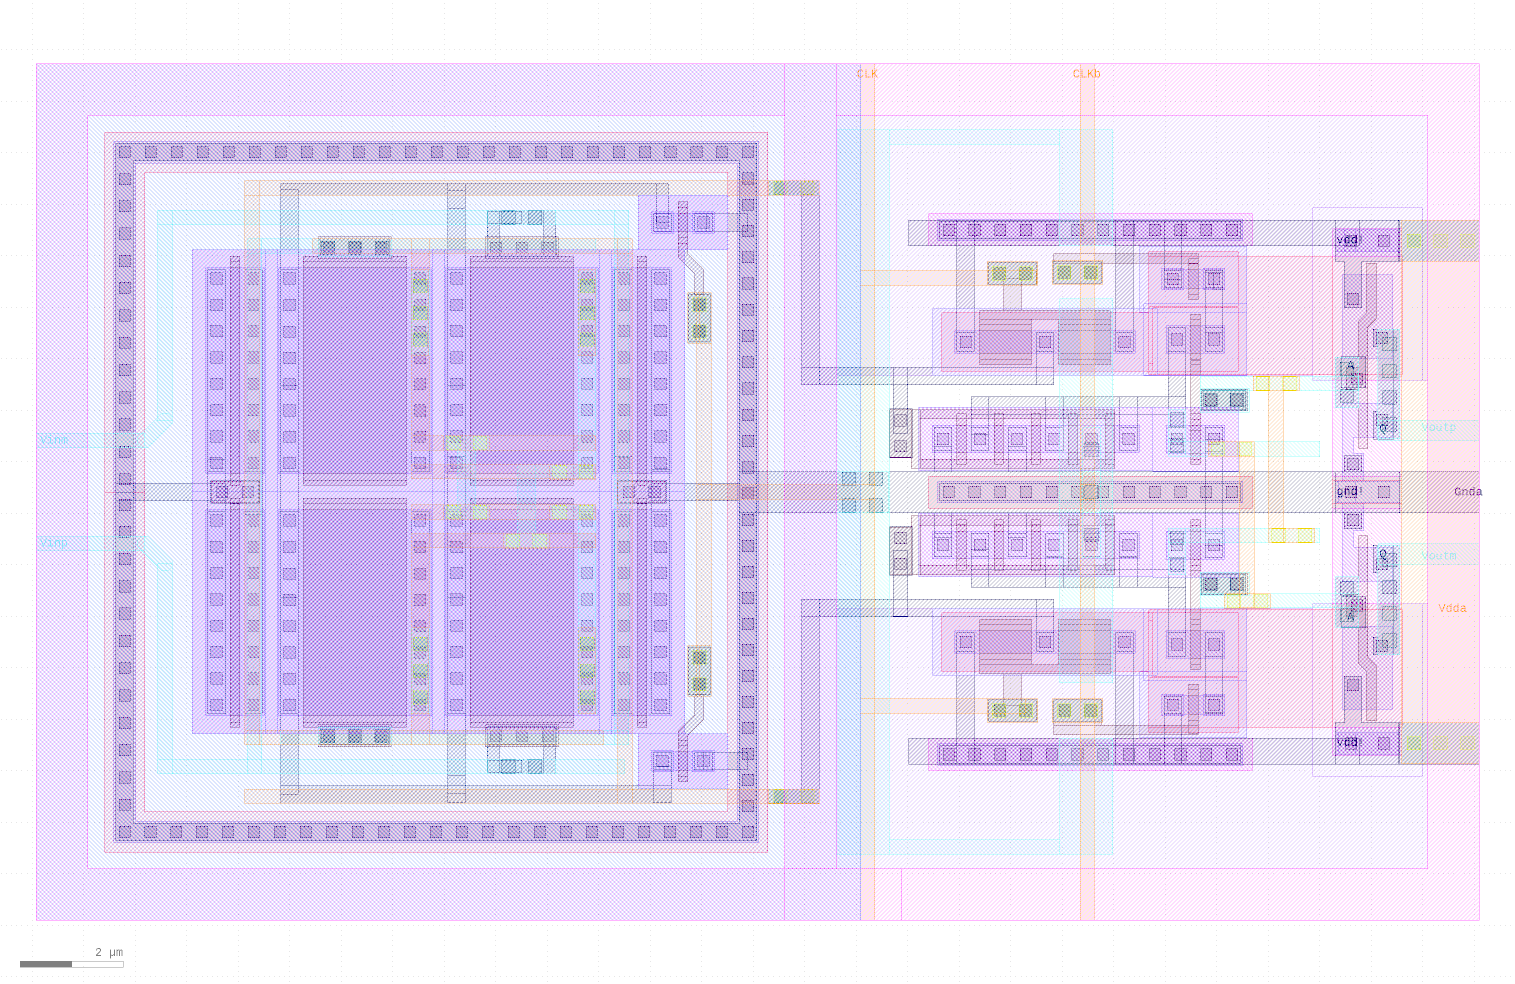
\includegraphics[width=\textwidth]{Chapter7/Figs/layout-slow-dtl.png}
        \subcaption{Double-Tail}
    \end{subfigure}
    \begin{subfigure}[b]{0.48\textwidth}
        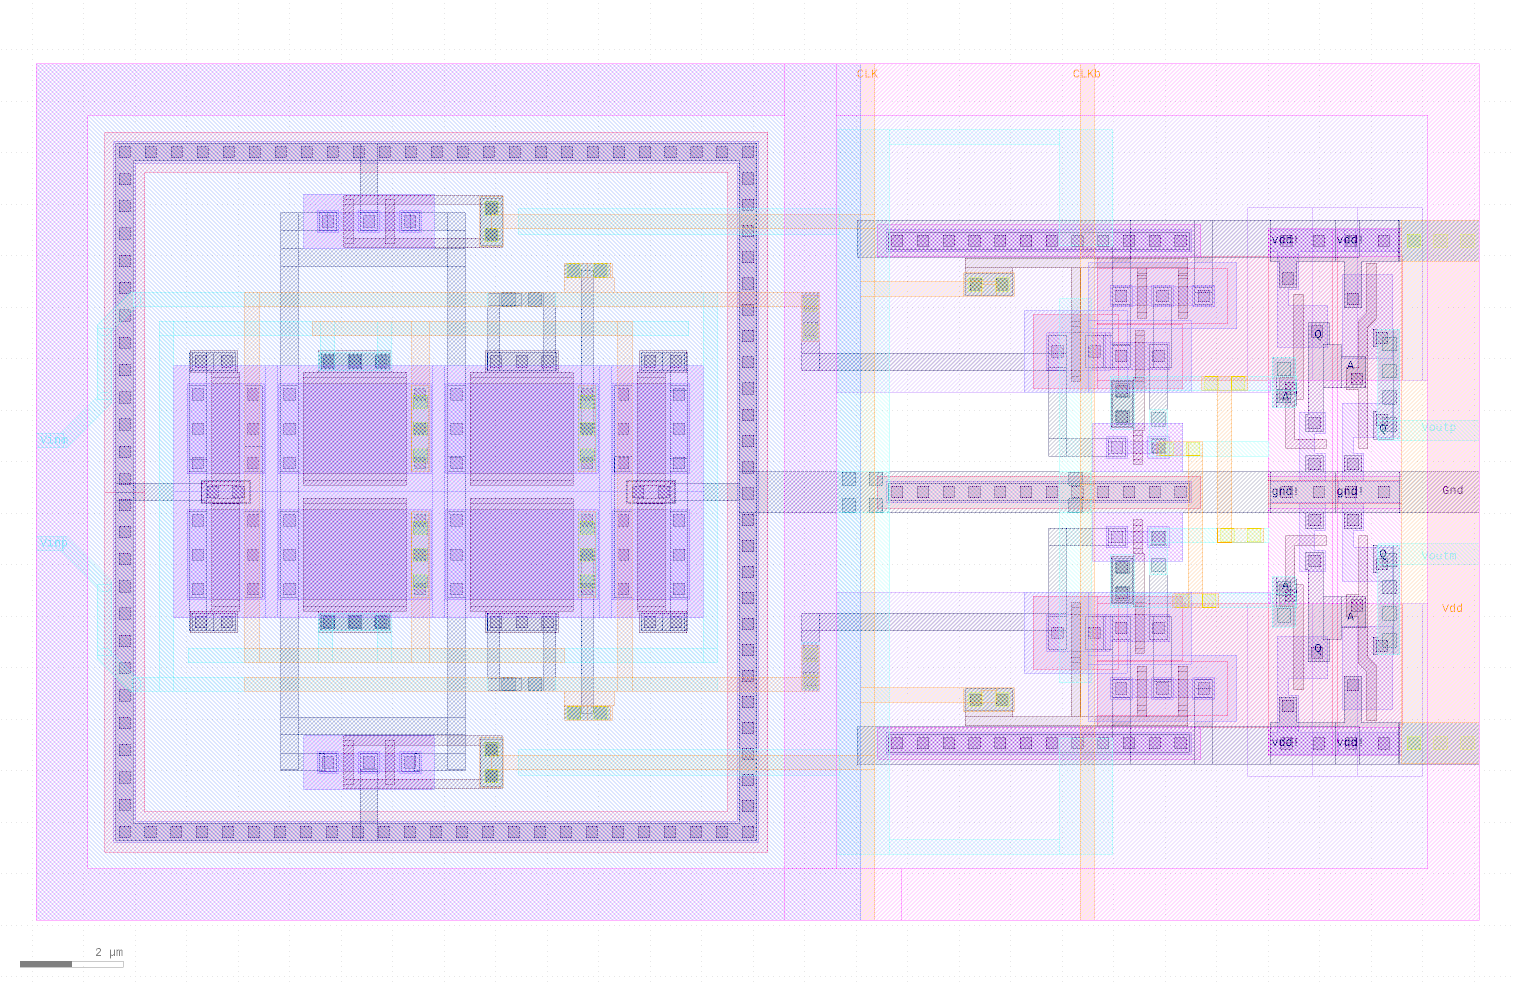
\includegraphics[width=\textwidth]{Chapter7/Figs/layout-slow-sa.png}
        \subcaption{Strong Arm}
    \end{subfigure}
    \caption{Layout of slow version of comparator designed made to respond in maximum 3 ns with a footprint of 28\(\mu m\) x 16\(\mu m\)}
    \label{fig:layout-comp}
\end{figure}

\figurename~\ref{fig:sim-comp}a represents the offset standard deviation over temperature. As agreed in the design phase, both architectures present a similar offset profile. As explained in~\cite{Fonseca2017}, the offset variation over temperature is tightly linked with the inverse of \(g_{m}/I_D\) variation.

\figurename~\ref{fig:sim-comp}b depicts the 3-\(\sigma \) delay variation over temperature of both architectures. For a differential input voltage of 800\(\mu \)V, the maximum delay increase with the temperature. The average response time of the SA latch varies from 2.3 ns to 2.53 ns. This represents a variation of 460 ppm/\(\degree \)C. While the standard deviation shrinks from 0.22 ns at -40\(\degree \)C to 0.15 ns +175\(\degree \)C, the maximum delay is almost constant over temperature. In the same condition, the DT latch exhibits an average time increase of 3333 ppm/\(\degree \)C. The main contributor to this temperature sensitivity is the differential pair transistor of the pre-amplifier as the design for low-offset gives more weight to the first stage. This value matches the results of a low-\(V_{th} \) transition frequency temperature sensitivity for the designed current of 20\(\mu \)A in differential pair transistors. However, the DT latch features a response time process variation increasing with the temperature as  0.15 ns at -40\(\degree \)C to 0.2 ns +175\(\degree \)C, close from the values of the SA latch.

In the \figurename~\ref{fig:sim-comp}c, the differential kickback is computed at the sample time since its effect will be seen when the decision is taken. While the temperature improves the differential kickback of the Strong ARM, the one of the double tail is more stable and is seven times smaller. Moreover, the kickback of the double tail is one order of magnitude lower than the kickback of the Strong ARM\@. So, the Double Tail is less prone to error. With a 600 µV of differential kickback for the Double Tail, this comparator introduces an error that is equivalent to 11.7 bit LSB for a differential input voltage of 1 V. In comparison the Strong ARM latch introduce an error equivalent to 9.4-bit LSB\@.

\figurename~\ref{fig:sim-comp}d presents the electrical simulation of comparator power consumption from -40\(\degree \)C to 175\(\degree \)C at 100 MHz. In both topologies, the power consumption increases as temperature rises. The Strong ARM average power consumption is 34 \(\mu \)W varying 592 ppm/\(\degree \)C over the temperature range while the Double Tail topology exhibits a 74 \(\mu \)W average power and 535 ppm/\(\degree \)C variation over the temperature range. Considering power consumption, one may conclude that Strong ARM has lower power consumption. However, Double Tail depicts a smaller variation \(\Delta P/P(T_0)\) with respect to the temperature.

\begin{figure}[ht]
    \centering
    \resizebox {0.9\textwidth} {!} {
        %% Creator: Matplotlib, PGF backend
%%
%% To include the figure in your LaTeX document, write
%%   \input{<filename>.pgf}
%%
%% Make sure the required packages are loaded in your preamble
%%   \usepackage{pgf}
%%
%% Figures using additional raster images can only be included by \input if
%% they are in the same directory as the main LaTeX file. For loading figures
%% from other directories you can use the `import` package
%%   \usepackage{import}
%% and then include the figures with
%%   \import{<path to file>}{<filename>.pgf}
%%
%% Matplotlib used the following preamble
%%   \usepackage{gensymb}
%%   \usepackage[utf8x]{inputenc}
%%   \usepackage[T1]{fontenc}
%%
\begingroup%
\makeatletter%
\begin{pgfpicture}%
\pgfpathrectangle{\pgfpointorigin}{\pgfqpoint{5.961700in}{5.051645in}}%
\pgfusepath{use as bounding box, clip}%
\begin{pgfscope}%
\pgfsetbuttcap%
\pgfsetmiterjoin%
\definecolor{currentfill}{rgb}{1.000000,1.000000,1.000000}%
\pgfsetfillcolor{currentfill}%
\pgfsetlinewidth{0.000000pt}%
\definecolor{currentstroke}{rgb}{1.000000,1.000000,1.000000}%
\pgfsetstrokecolor{currentstroke}%
\pgfsetdash{}{0pt}%
\pgfpathmoveto{\pgfqpoint{0.000000in}{0.000000in}}%
\pgfpathlineto{\pgfqpoint{5.961700in}{0.000000in}}%
\pgfpathlineto{\pgfqpoint{5.961700in}{5.051645in}}%
\pgfpathlineto{\pgfqpoint{0.000000in}{5.051645in}}%
\pgfpathclose%
\pgfusepath{fill}%
\end{pgfscope}%
\begin{pgfscope}%
\pgfsetbuttcap%
\pgfsetmiterjoin%
\definecolor{currentfill}{rgb}{1.000000,1.000000,1.000000}%
\pgfsetfillcolor{currentfill}%
\pgfsetlinewidth{0.000000pt}%
\definecolor{currentstroke}{rgb}{0.000000,0.000000,0.000000}%
\pgfsetstrokecolor{currentstroke}%
\pgfsetstrokeopacity{0.000000}%
\pgfsetdash{}{0pt}%
\pgfpathmoveto{\pgfqpoint{0.610776in}{3.198687in}}%
\pgfpathlineto{\pgfqpoint{2.852125in}{3.198687in}}%
\pgfpathlineto{\pgfqpoint{2.852125in}{4.698266in}}%
\pgfpathlineto{\pgfqpoint{0.610776in}{4.698266in}}%
\pgfpathclose%
\pgfusepath{fill}%
\end{pgfscope}%
\begin{pgfscope}%
\pgfpathrectangle{\pgfqpoint{0.610776in}{3.198687in}}{\pgfqpoint{2.241349in}{1.499579in}} %
\pgfusepath{clip}%
\pgfsetbuttcap%
\pgfsetroundjoin%
\definecolor{currentfill}{rgb}{0.666667,0.223529,0.223529}%
\pgfsetfillcolor{currentfill}%
\pgfsetfillopacity{0.250000}%
\pgfsetlinewidth{0.000000pt}%
\definecolor{currentstroke}{rgb}{0.000000,0.000000,0.000000}%
\pgfsetstrokecolor{currentstroke}%
\pgfsetdash{}{0pt}%
\pgfpathmoveto{\pgfqpoint{0.610776in}{4.539027in}}%
\pgfpathlineto{\pgfqpoint{0.610776in}{3.634114in}}%
\pgfpathlineto{\pgfqpoint{0.767149in}{3.634360in}}%
\pgfpathlineto{\pgfqpoint{1.027771in}{3.630945in}}%
\pgfpathlineto{\pgfqpoint{1.288393in}{3.629123in}}%
\pgfpathlineto{\pgfqpoint{1.309243in}{3.629770in}}%
\pgfpathlineto{\pgfqpoint{1.674114in}{3.610223in}}%
\pgfpathlineto{\pgfqpoint{1.913886in}{3.604355in}}%
\pgfpathlineto{\pgfqpoint{2.070259in}{3.602096in}}%
\pgfpathlineto{\pgfqpoint{2.330881in}{3.587250in}}%
\pgfpathlineto{\pgfqpoint{2.591503in}{3.572929in}}%
\pgfpathlineto{\pgfqpoint{2.852125in}{3.551435in}}%
\pgfpathlineto{\pgfqpoint{2.852125in}{4.661889in}}%
\pgfpathlineto{\pgfqpoint{2.852125in}{4.661889in}}%
\pgfpathlineto{\pgfqpoint{2.591503in}{4.638487in}}%
\pgfpathlineto{\pgfqpoint{2.330881in}{4.619648in}}%
\pgfpathlineto{\pgfqpoint{2.070259in}{4.597597in}}%
\pgfpathlineto{\pgfqpoint{1.913886in}{4.593630in}}%
\pgfpathlineto{\pgfqpoint{1.674114in}{4.584209in}}%
\pgfpathlineto{\pgfqpoint{1.309243in}{4.554554in}}%
\pgfpathlineto{\pgfqpoint{1.288393in}{4.554712in}}%
\pgfpathlineto{\pgfqpoint{1.027771in}{4.548810in}}%
\pgfpathlineto{\pgfqpoint{0.767149in}{4.540409in}}%
\pgfpathlineto{\pgfqpoint{0.610776in}{4.539027in}}%
\pgfpathclose%
\pgfusepath{fill}%
\end{pgfscope}%
\begin{pgfscope}%
\pgfpathrectangle{\pgfqpoint{0.610776in}{3.198687in}}{\pgfqpoint{2.241349in}{1.499579in}} %
\pgfusepath{clip}%
\pgfsetbuttcap%
\pgfsetroundjoin%
\definecolor{currentfill}{rgb}{0.666667,0.592157,0.223529}%
\pgfsetfillcolor{currentfill}%
\pgfsetfillopacity{0.250000}%
\pgfsetlinewidth{0.000000pt}%
\definecolor{currentstroke}{rgb}{0.000000,0.000000,0.000000}%
\pgfsetstrokecolor{currentstroke}%
\pgfsetdash{}{0pt}%
\pgfpathmoveto{\pgfqpoint{0.610776in}{4.570555in}}%
\pgfpathlineto{\pgfqpoint{0.610776in}{3.465656in}}%
\pgfpathlineto{\pgfqpoint{0.767149in}{3.455552in}}%
\pgfpathlineto{\pgfqpoint{1.027771in}{3.439680in}}%
\pgfpathlineto{\pgfqpoint{1.288393in}{3.414952in}}%
\pgfpathlineto{\pgfqpoint{1.309243in}{3.414363in}}%
\pgfpathlineto{\pgfqpoint{1.674114in}{3.382064in}}%
\pgfpathlineto{\pgfqpoint{1.913886in}{3.355655in}}%
\pgfpathlineto{\pgfqpoint{2.070259in}{3.340597in}}%
\pgfpathlineto{\pgfqpoint{2.330881in}{3.315077in}}%
\pgfpathlineto{\pgfqpoint{2.591503in}{3.288192in}}%
\pgfpathlineto{\pgfqpoint{2.852125in}{3.259496in}}%
\pgfpathlineto{\pgfqpoint{2.852125in}{4.674611in}}%
\pgfpathlineto{\pgfqpoint{2.852125in}{4.674611in}}%
\pgfpathlineto{\pgfqpoint{2.591503in}{4.659008in}}%
\pgfpathlineto{\pgfqpoint{2.330881in}{4.644828in}}%
\pgfpathlineto{\pgfqpoint{2.070259in}{4.633301in}}%
\pgfpathlineto{\pgfqpoint{1.913886in}{4.626978in}}%
\pgfpathlineto{\pgfqpoint{1.674114in}{4.614966in}}%
\pgfpathlineto{\pgfqpoint{1.309243in}{4.598744in}}%
\pgfpathlineto{\pgfqpoint{1.288393in}{4.599024in}}%
\pgfpathlineto{\pgfqpoint{1.027771in}{4.584662in}}%
\pgfpathlineto{\pgfqpoint{0.767149in}{4.575577in}}%
\pgfpathlineto{\pgfqpoint{0.610776in}{4.570555in}}%
\pgfpathclose%
\pgfusepath{fill}%
\end{pgfscope}%
\begin{pgfscope}%
\pgfsetbuttcap%
\pgfsetroundjoin%
\definecolor{currentfill}{rgb}{0.000000,0.000000,0.000000}%
\pgfsetfillcolor{currentfill}%
\pgfsetlinewidth{0.803000pt}%
\definecolor{currentstroke}{rgb}{0.000000,0.000000,0.000000}%
\pgfsetstrokecolor{currentstroke}%
\pgfsetdash{}{0pt}%
\pgfsys@defobject{currentmarker}{\pgfqpoint{0.000000in}{-0.048611in}}{\pgfqpoint{0.000000in}{0.000000in}}{%
\pgfpathmoveto{\pgfqpoint{0.000000in}{0.000000in}}%
\pgfpathlineto{\pgfqpoint{0.000000in}{-0.048611in}}%
\pgfusepath{stroke,fill}%
}%
\begin{pgfscope}%
\pgfsys@transformshift{0.610776in}{3.198687in}%
\pgfsys@useobject{currentmarker}{}%
\end{pgfscope}%
\end{pgfscope}%
\begin{pgfscope}%
\pgftext[x=0.610776in,y=3.101465in,,top]{\fontsize{10.000000}{12.000000}\selectfont \(\displaystyle -40\)}%
\end{pgfscope}%
\begin{pgfscope}%
\pgfsetbuttcap%
\pgfsetroundjoin%
\definecolor{currentfill}{rgb}{0.000000,0.000000,0.000000}%
\pgfsetfillcolor{currentfill}%
\pgfsetlinewidth{0.803000pt}%
\definecolor{currentstroke}{rgb}{0.000000,0.000000,0.000000}%
\pgfsetstrokecolor{currentstroke}%
\pgfsetdash{}{0pt}%
\pgfsys@defobject{currentmarker}{\pgfqpoint{0.000000in}{-0.048611in}}{\pgfqpoint{0.000000in}{0.000000in}}{%
\pgfpathmoveto{\pgfqpoint{0.000000in}{0.000000in}}%
\pgfpathlineto{\pgfqpoint{0.000000in}{-0.048611in}}%
\pgfusepath{stroke,fill}%
}%
\begin{pgfscope}%
\pgfsys@transformshift{1.027771in}{3.198687in}%
\pgfsys@useobject{currentmarker}{}%
\end{pgfscope}%
\end{pgfscope}%
\begin{pgfscope}%
\pgftext[x=1.027771in,y=3.101465in,,top]{\fontsize{10.000000}{12.000000}\selectfont \(\displaystyle 0\)}%
\end{pgfscope}%
\begin{pgfscope}%
\pgfsetbuttcap%
\pgfsetroundjoin%
\definecolor{currentfill}{rgb}{0.000000,0.000000,0.000000}%
\pgfsetfillcolor{currentfill}%
\pgfsetlinewidth{0.803000pt}%
\definecolor{currentstroke}{rgb}{0.000000,0.000000,0.000000}%
\pgfsetstrokecolor{currentstroke}%
\pgfsetdash{}{0pt}%
\pgfsys@defobject{currentmarker}{\pgfqpoint{0.000000in}{-0.048611in}}{\pgfqpoint{0.000000in}{0.000000in}}{%
\pgfpathmoveto{\pgfqpoint{0.000000in}{0.000000in}}%
\pgfpathlineto{\pgfqpoint{0.000000in}{-0.048611in}}%
\pgfusepath{stroke,fill}%
}%
\begin{pgfscope}%
\pgfsys@transformshift{1.309243in}{3.198687in}%
\pgfsys@useobject{currentmarker}{}%
\end{pgfscope}%
\end{pgfscope}%
\begin{pgfscope}%
\pgftext[x=1.309243in,y=3.101465in,,top]{\fontsize{10.000000}{12.000000}\selectfont \(\displaystyle 27\)}%
\end{pgfscope}%
\begin{pgfscope}%
\pgfsetbuttcap%
\pgfsetroundjoin%
\definecolor{currentfill}{rgb}{0.000000,0.000000,0.000000}%
\pgfsetfillcolor{currentfill}%
\pgfsetlinewidth{0.803000pt}%
\definecolor{currentstroke}{rgb}{0.000000,0.000000,0.000000}%
\pgfsetstrokecolor{currentstroke}%
\pgfsetdash{}{0pt}%
\pgfsys@defobject{currentmarker}{\pgfqpoint{0.000000in}{-0.048611in}}{\pgfqpoint{0.000000in}{0.000000in}}{%
\pgfpathmoveto{\pgfqpoint{0.000000in}{0.000000in}}%
\pgfpathlineto{\pgfqpoint{0.000000in}{-0.048611in}}%
\pgfusepath{stroke,fill}%
}%
\begin{pgfscope}%
\pgfsys@transformshift{1.913886in}{3.198687in}%
\pgfsys@useobject{currentmarker}{}%
\end{pgfscope}%
\end{pgfscope}%
\begin{pgfscope}%
\pgftext[x=1.913886in,y=3.101465in,,top]{\fontsize{10.000000}{12.000000}\selectfont \(\displaystyle 85\)}%
\end{pgfscope}%
\begin{pgfscope}%
\pgfsetbuttcap%
\pgfsetroundjoin%
\definecolor{currentfill}{rgb}{0.000000,0.000000,0.000000}%
\pgfsetfillcolor{currentfill}%
\pgfsetlinewidth{0.803000pt}%
\definecolor{currentstroke}{rgb}{0.000000,0.000000,0.000000}%
\pgfsetstrokecolor{currentstroke}%
\pgfsetdash{}{0pt}%
\pgfsys@defobject{currentmarker}{\pgfqpoint{0.000000in}{-0.048611in}}{\pgfqpoint{0.000000in}{0.000000in}}{%
\pgfpathmoveto{\pgfqpoint{0.000000in}{0.000000in}}%
\pgfpathlineto{\pgfqpoint{0.000000in}{-0.048611in}}%
\pgfusepath{stroke,fill}%
}%
\begin{pgfscope}%
\pgfsys@transformshift{2.591503in}{3.198687in}%
\pgfsys@useobject{currentmarker}{}%
\end{pgfscope}%
\end{pgfscope}%
\begin{pgfscope}%
\pgftext[x=2.591503in,y=3.101465in,,top]{\fontsize{10.000000}{12.000000}\selectfont \(\displaystyle 150\)}%
\end{pgfscope}%
\begin{pgfscope}%
\pgfsetbuttcap%
\pgfsetroundjoin%
\definecolor{currentfill}{rgb}{0.000000,0.000000,0.000000}%
\pgfsetfillcolor{currentfill}%
\pgfsetlinewidth{0.803000pt}%
\definecolor{currentstroke}{rgb}{0.000000,0.000000,0.000000}%
\pgfsetstrokecolor{currentstroke}%
\pgfsetdash{}{0pt}%
\pgfsys@defobject{currentmarker}{\pgfqpoint{0.000000in}{-0.048611in}}{\pgfqpoint{0.000000in}{0.000000in}}{%
\pgfpathmoveto{\pgfqpoint{0.000000in}{0.000000in}}%
\pgfpathlineto{\pgfqpoint{0.000000in}{-0.048611in}}%
\pgfusepath{stroke,fill}%
}%
\begin{pgfscope}%
\pgfsys@transformshift{2.852125in}{3.198687in}%
\pgfsys@useobject{currentmarker}{}%
\end{pgfscope}%
\end{pgfscope}%
\begin{pgfscope}%
\pgftext[x=2.852125in,y=3.101465in,,top]{\fontsize{10.000000}{12.000000}\selectfont \(\displaystyle 175\)}%
\end{pgfscope}%
\begin{pgfscope}%
\pgftext[x=1.731451in,y=2.923254in,,top]{\fontsize{8.000000}{9.600000}\selectfont Temperature [\(\displaystyle \degree\)C]}%
\end{pgfscope}%
\begin{pgfscope}%
\pgfsetbuttcap%
\pgfsetroundjoin%
\definecolor{currentfill}{rgb}{0.000000,0.000000,0.000000}%
\pgfsetfillcolor{currentfill}%
\pgfsetlinewidth{0.803000pt}%
\definecolor{currentstroke}{rgb}{0.000000,0.000000,0.000000}%
\pgfsetstrokecolor{currentstroke}%
\pgfsetdash{}{0pt}%
\pgfsys@defobject{currentmarker}{\pgfqpoint{-0.048611in}{0.000000in}}{\pgfqpoint{0.000000in}{0.000000in}}{%
\pgfpathmoveto{\pgfqpoint{0.000000in}{0.000000in}}%
\pgfpathlineto{\pgfqpoint{-0.048611in}{0.000000in}}%
\pgfusepath{stroke,fill}%
}%
\begin{pgfscope}%
\pgfsys@transformshift{0.610776in}{3.487068in}%
\pgfsys@useobject{currentmarker}{}%
\end{pgfscope}%
\end{pgfscope}%
\begin{pgfscope}%
\pgftext[x=0.266640in,y=3.439240in,left,base]{\fontsize{10.000000}{12.000000}\selectfont \(\displaystyle -10\)}%
\end{pgfscope}%
\begin{pgfscope}%
\pgfsetbuttcap%
\pgfsetroundjoin%
\definecolor{currentfill}{rgb}{0.000000,0.000000,0.000000}%
\pgfsetfillcolor{currentfill}%
\pgfsetlinewidth{0.803000pt}%
\definecolor{currentstroke}{rgb}{0.000000,0.000000,0.000000}%
\pgfsetstrokecolor{currentstroke}%
\pgfsetdash{}{0pt}%
\pgfsys@defobject{currentmarker}{\pgfqpoint{-0.048611in}{0.000000in}}{\pgfqpoint{0.000000in}{0.000000in}}{%
\pgfpathmoveto{\pgfqpoint{0.000000in}{0.000000in}}%
\pgfpathlineto{\pgfqpoint{-0.048611in}{0.000000in}}%
\pgfusepath{stroke,fill}%
}%
\begin{pgfscope}%
\pgfsys@transformshift{0.610776in}{4.063829in}%
\pgfsys@useobject{currentmarker}{}%
\end{pgfscope}%
\end{pgfscope}%
\begin{pgfscope}%
\pgftext[x=0.444109in,y=4.016001in,left,base]{\fontsize{10.000000}{12.000000}\selectfont \(\displaystyle 0\)}%
\end{pgfscope}%
\begin{pgfscope}%
\pgfsetbuttcap%
\pgfsetroundjoin%
\definecolor{currentfill}{rgb}{0.000000,0.000000,0.000000}%
\pgfsetfillcolor{currentfill}%
\pgfsetlinewidth{0.803000pt}%
\definecolor{currentstroke}{rgb}{0.000000,0.000000,0.000000}%
\pgfsetstrokecolor{currentstroke}%
\pgfsetdash{}{0pt}%
\pgfsys@defobject{currentmarker}{\pgfqpoint{-0.048611in}{0.000000in}}{\pgfqpoint{0.000000in}{0.000000in}}{%
\pgfpathmoveto{\pgfqpoint{0.000000in}{0.000000in}}%
\pgfpathlineto{\pgfqpoint{-0.048611in}{0.000000in}}%
\pgfusepath{stroke,fill}%
}%
\begin{pgfscope}%
\pgfsys@transformshift{0.610776in}{4.640590in}%
\pgfsys@useobject{currentmarker}{}%
\end{pgfscope}%
\end{pgfscope}%
\begin{pgfscope}%
\pgftext[x=0.374665in,y=4.592763in,left,base]{\fontsize{10.000000}{12.000000}\selectfont \(\displaystyle 10\)}%
\end{pgfscope}%
\begin{pgfscope}%
\pgftext[x=0.211084in,y=3.948477in,,bottom,rotate=90.000000]{\fontsize{8.000000}{9.600000}\selectfont Input Referred Offset [mV]}%
\end{pgfscope}%
\begin{pgfscope}%
\pgfpathrectangle{\pgfqpoint{0.610776in}{3.198687in}}{\pgfqpoint{2.241349in}{1.499579in}} %
\pgfusepath{clip}%
\pgfsetrectcap%
\pgfsetroundjoin%
\pgfsetlinewidth{2.007500pt}%
\definecolor{currentstroke}{rgb}{0.666667,0.223529,0.223529}%
\pgfsetstrokecolor{currentstroke}%
\pgfsetdash{}{0pt}%
\pgfpathmoveto{\pgfqpoint{0.610776in}{4.086570in}}%
\pgfpathlineto{\pgfqpoint{0.767149in}{4.087385in}}%
\pgfpathlineto{\pgfqpoint{1.027771in}{4.089877in}}%
\pgfpathlineto{\pgfqpoint{1.288393in}{4.091918in}}%
\pgfpathlineto{\pgfqpoint{1.309243in}{4.092162in}}%
\pgfpathlineto{\pgfqpoint{1.674114in}{4.097216in}}%
\pgfpathlineto{\pgfqpoint{1.913886in}{4.098992in}}%
\pgfpathlineto{\pgfqpoint{2.070259in}{4.099847in}}%
\pgfpathlineto{\pgfqpoint{2.330881in}{4.103449in}}%
\pgfpathlineto{\pgfqpoint{2.591503in}{4.105708in}}%
\pgfpathlineto{\pgfqpoint{2.852125in}{4.106662in}}%
\pgfusepath{stroke}%
\end{pgfscope}%
\begin{pgfscope}%
\pgfpathrectangle{\pgfqpoint{0.610776in}{3.198687in}}{\pgfqpoint{2.241349in}{1.499579in}} %
\pgfusepath{clip}%
\pgfsetrectcap%
\pgfsetroundjoin%
\pgfsetlinewidth{2.007500pt}%
\definecolor{currentstroke}{rgb}{0.666667,0.592157,0.223529}%
\pgfsetstrokecolor{currentstroke}%
\pgfsetdash{}{0pt}%
\pgfpathmoveto{\pgfqpoint{0.610776in}{4.018106in}}%
\pgfpathlineto{\pgfqpoint{0.767149in}{4.015565in}}%
\pgfpathlineto{\pgfqpoint{1.027771in}{4.012171in}}%
\pgfpathlineto{\pgfqpoint{1.288393in}{4.006988in}}%
\pgfpathlineto{\pgfqpoint{1.309243in}{4.006553in}}%
\pgfpathlineto{\pgfqpoint{1.674114in}{3.998515in}}%
\pgfpathlineto{\pgfqpoint{1.913886in}{3.991316in}}%
\pgfpathlineto{\pgfqpoint{2.070259in}{3.986949in}}%
\pgfpathlineto{\pgfqpoint{2.330881in}{3.979953in}}%
\pgfpathlineto{\pgfqpoint{2.591503in}{3.973600in}}%
\pgfpathlineto{\pgfqpoint{2.852125in}{3.967053in}}%
\pgfusepath{stroke}%
\end{pgfscope}%
\begin{pgfscope}%
\pgfsetrectcap%
\pgfsetmiterjoin%
\pgfsetlinewidth{0.803000pt}%
\definecolor{currentstroke}{rgb}{0.000000,0.000000,0.000000}%
\pgfsetstrokecolor{currentstroke}%
\pgfsetdash{}{0pt}%
\pgfpathmoveto{\pgfqpoint{0.610776in}{3.198687in}}%
\pgfpathlineto{\pgfqpoint{0.610776in}{4.698266in}}%
\pgfusepath{stroke}%
\end{pgfscope}%
\begin{pgfscope}%
\pgfsetrectcap%
\pgfsetmiterjoin%
\pgfsetlinewidth{0.803000pt}%
\definecolor{currentstroke}{rgb}{0.000000,0.000000,0.000000}%
\pgfsetstrokecolor{currentstroke}%
\pgfsetdash{}{0pt}%
\pgfpathmoveto{\pgfqpoint{2.852125in}{3.198687in}}%
\pgfpathlineto{\pgfqpoint{2.852125in}{4.698266in}}%
\pgfusepath{stroke}%
\end{pgfscope}%
\begin{pgfscope}%
\pgfsetrectcap%
\pgfsetmiterjoin%
\pgfsetlinewidth{0.803000pt}%
\definecolor{currentstroke}{rgb}{0.000000,0.000000,0.000000}%
\pgfsetstrokecolor{currentstroke}%
\pgfsetdash{}{0pt}%
\pgfpathmoveto{\pgfqpoint{0.610776in}{3.198687in}}%
\pgfpathlineto{\pgfqpoint{2.852125in}{3.198687in}}%
\pgfusepath{stroke}%
\end{pgfscope}%
\begin{pgfscope}%
\pgfsetrectcap%
\pgfsetmiterjoin%
\pgfsetlinewidth{0.803000pt}%
\definecolor{currentstroke}{rgb}{0.000000,0.000000,0.000000}%
\pgfsetstrokecolor{currentstroke}%
\pgfsetdash{}{0pt}%
\pgfpathmoveto{\pgfqpoint{0.610776in}{4.698266in}}%
\pgfpathlineto{\pgfqpoint{2.852125in}{4.698266in}}%
\pgfusepath{stroke}%
\end{pgfscope}%
\begin{pgfscope}%
\pgftext[x=1.731451in,y=2.562222in,,base]{\fontsize{9.600000}{11.520000}\selectfont a) input referred offset}%
\end{pgfscope}%
\begin{pgfscope}%
\pgfsetbuttcap%
\pgfsetmiterjoin%
\definecolor{currentfill}{rgb}{1.000000,1.000000,1.000000}%
\pgfsetfillcolor{currentfill}%
\pgfsetlinewidth{0.000000pt}%
\definecolor{currentstroke}{rgb}{0.000000,0.000000,0.000000}%
\pgfsetstrokecolor{currentstroke}%
\pgfsetstrokeopacity{0.000000}%
\pgfsetdash{}{0pt}%
\pgfpathmoveto{\pgfqpoint{3.516184in}{3.198687in}}%
\pgfpathlineto{\pgfqpoint{5.757533in}{3.198687in}}%
\pgfpathlineto{\pgfqpoint{5.757533in}{4.698266in}}%
\pgfpathlineto{\pgfqpoint{3.516184in}{4.698266in}}%
\pgfpathclose%
\pgfusepath{fill}%
\end{pgfscope}%
\begin{pgfscope}%
\pgfpathrectangle{\pgfqpoint{3.516184in}{3.198687in}}{\pgfqpoint{2.241349in}{1.499579in}} %
\pgfusepath{clip}%
\pgfsetbuttcap%
\pgfsetroundjoin%
\definecolor{currentfill}{rgb}{0.666667,0.223529,0.223529}%
\pgfsetfillcolor{currentfill}%
\pgfsetfillopacity{0.250000}%
\pgfsetlinewidth{0.000000pt}%
\definecolor{currentstroke}{rgb}{0.000000,0.000000,0.000000}%
\pgfsetstrokecolor{currentstroke}%
\pgfsetdash{}{0pt}%
\pgfpathmoveto{\pgfqpoint{3.516184in}{3.539243in}}%
\pgfpathlineto{\pgfqpoint{3.516184in}{3.277609in}}%
\pgfpathlineto{\pgfqpoint{3.672557in}{3.317956in}}%
\pgfpathlineto{\pgfqpoint{3.933179in}{3.359485in}}%
\pgfpathlineto{\pgfqpoint{4.193801in}{3.451937in}}%
\pgfpathlineto{\pgfqpoint{4.214650in}{3.471116in}}%
\pgfpathlineto{\pgfqpoint{4.579521in}{3.518896in}}%
\pgfpathlineto{\pgfqpoint{4.819293in}{3.631973in}}%
\pgfpathlineto{\pgfqpoint{4.975667in}{3.649663in}}%
\pgfpathlineto{\pgfqpoint{5.236289in}{3.681378in}}%
\pgfpathlineto{\pgfqpoint{5.496911in}{3.809706in}}%
\pgfpathlineto{\pgfqpoint{5.757533in}{3.885412in}}%
\pgfpathlineto{\pgfqpoint{5.757533in}{4.306614in}}%
\pgfpathlineto{\pgfqpoint{5.757533in}{4.306614in}}%
\pgfpathlineto{\pgfqpoint{5.496911in}{4.198292in}}%
\pgfpathlineto{\pgfqpoint{5.236289in}{4.169643in}}%
\pgfpathlineto{\pgfqpoint{4.975667in}{4.051655in}}%
\pgfpathlineto{\pgfqpoint{4.819293in}{3.954162in}}%
\pgfpathlineto{\pgfqpoint{4.579521in}{3.936611in}}%
\pgfpathlineto{\pgfqpoint{4.214650in}{3.772666in}}%
\pgfpathlineto{\pgfqpoint{4.193801in}{3.781183in}}%
\pgfpathlineto{\pgfqpoint{3.933179in}{3.716778in}}%
\pgfpathlineto{\pgfqpoint{3.672557in}{3.597478in}}%
\pgfpathlineto{\pgfqpoint{3.516184in}{3.539243in}}%
\pgfpathclose%
\pgfusepath{fill}%
\end{pgfscope}%
\begin{pgfscope}%
\pgfpathrectangle{\pgfqpoint{3.516184in}{3.198687in}}{\pgfqpoint{2.241349in}{1.499579in}} %
\pgfusepath{clip}%
\pgfsetbuttcap%
\pgfsetroundjoin%
\definecolor{currentfill}{rgb}{0.666667,0.592157,0.223529}%
\pgfsetfillcolor{currentfill}%
\pgfsetfillopacity{0.250000}%
\pgfsetlinewidth{0.000000pt}%
\definecolor{currentstroke}{rgb}{0.000000,0.000000,0.000000}%
\pgfsetstrokecolor{currentstroke}%
\pgfsetdash{}{0pt}%
\pgfpathmoveto{\pgfqpoint{3.516184in}{3.487371in}}%
\pgfpathlineto{\pgfqpoint{3.516184in}{3.221256in}}%
\pgfpathlineto{\pgfqpoint{3.672557in}{3.245471in}}%
\pgfpathlineto{\pgfqpoint{3.933179in}{3.322649in}}%
\pgfpathlineto{\pgfqpoint{4.193801in}{3.390911in}}%
\pgfpathlineto{\pgfqpoint{4.214650in}{3.386222in}}%
\pgfpathlineto{\pgfqpoint{4.579521in}{3.495915in}}%
\pgfpathlineto{\pgfqpoint{4.819293in}{3.541192in}}%
\pgfpathlineto{\pgfqpoint{4.975667in}{3.570394in}}%
\pgfpathlineto{\pgfqpoint{5.236289in}{3.653193in}}%
\pgfpathlineto{\pgfqpoint{5.496911in}{3.717440in}}%
\pgfpathlineto{\pgfqpoint{5.757533in}{3.764508in}}%
\pgfpathlineto{\pgfqpoint{5.757533in}{4.218581in}}%
\pgfpathlineto{\pgfqpoint{5.757533in}{4.218581in}}%
\pgfpathlineto{\pgfqpoint{5.496911in}{4.124509in}}%
\pgfpathlineto{\pgfqpoint{5.236289in}{4.064710in}}%
\pgfpathlineto{\pgfqpoint{4.975667in}{4.005110in}}%
\pgfpathlineto{\pgfqpoint{4.819293in}{3.940033in}}%
\pgfpathlineto{\pgfqpoint{4.579521in}{3.827794in}}%
\pgfpathlineto{\pgfqpoint{4.214650in}{3.737009in}}%
\pgfpathlineto{\pgfqpoint{4.193801in}{3.722647in}}%
\pgfpathlineto{\pgfqpoint{3.933179in}{3.640247in}}%
\pgfpathlineto{\pgfqpoint{3.672557in}{3.570811in}}%
\pgfpathlineto{\pgfqpoint{3.516184in}{3.487371in}}%
\pgfpathclose%
\pgfusepath{fill}%
\end{pgfscope}%
\begin{pgfscope}%
\pgfsetbuttcap%
\pgfsetroundjoin%
\definecolor{currentfill}{rgb}{0.000000,0.000000,0.000000}%
\pgfsetfillcolor{currentfill}%
\pgfsetlinewidth{0.803000pt}%
\definecolor{currentstroke}{rgb}{0.000000,0.000000,0.000000}%
\pgfsetstrokecolor{currentstroke}%
\pgfsetdash{}{0pt}%
\pgfsys@defobject{currentmarker}{\pgfqpoint{0.000000in}{-0.048611in}}{\pgfqpoint{0.000000in}{0.000000in}}{%
\pgfpathmoveto{\pgfqpoint{0.000000in}{0.000000in}}%
\pgfpathlineto{\pgfqpoint{0.000000in}{-0.048611in}}%
\pgfusepath{stroke,fill}%
}%
\begin{pgfscope}%
\pgfsys@transformshift{3.516184in}{3.198687in}%
\pgfsys@useobject{currentmarker}{}%
\end{pgfscope}%
\end{pgfscope}%
\begin{pgfscope}%
\pgftext[x=3.516184in,y=3.101465in,,top]{\fontsize{10.000000}{12.000000}\selectfont \(\displaystyle -40\)}%
\end{pgfscope}%
\begin{pgfscope}%
\pgfsetbuttcap%
\pgfsetroundjoin%
\definecolor{currentfill}{rgb}{0.000000,0.000000,0.000000}%
\pgfsetfillcolor{currentfill}%
\pgfsetlinewidth{0.803000pt}%
\definecolor{currentstroke}{rgb}{0.000000,0.000000,0.000000}%
\pgfsetstrokecolor{currentstroke}%
\pgfsetdash{}{0pt}%
\pgfsys@defobject{currentmarker}{\pgfqpoint{0.000000in}{-0.048611in}}{\pgfqpoint{0.000000in}{0.000000in}}{%
\pgfpathmoveto{\pgfqpoint{0.000000in}{0.000000in}}%
\pgfpathlineto{\pgfqpoint{0.000000in}{-0.048611in}}%
\pgfusepath{stroke,fill}%
}%
\begin{pgfscope}%
\pgfsys@transformshift{3.933179in}{3.198687in}%
\pgfsys@useobject{currentmarker}{}%
\end{pgfscope}%
\end{pgfscope}%
\begin{pgfscope}%
\pgftext[x=3.933179in,y=3.101465in,,top]{\fontsize{10.000000}{12.000000}\selectfont \(\displaystyle 0\)}%
\end{pgfscope}%
\begin{pgfscope}%
\pgfsetbuttcap%
\pgfsetroundjoin%
\definecolor{currentfill}{rgb}{0.000000,0.000000,0.000000}%
\pgfsetfillcolor{currentfill}%
\pgfsetlinewidth{0.803000pt}%
\definecolor{currentstroke}{rgb}{0.000000,0.000000,0.000000}%
\pgfsetstrokecolor{currentstroke}%
\pgfsetdash{}{0pt}%
\pgfsys@defobject{currentmarker}{\pgfqpoint{0.000000in}{-0.048611in}}{\pgfqpoint{0.000000in}{0.000000in}}{%
\pgfpathmoveto{\pgfqpoint{0.000000in}{0.000000in}}%
\pgfpathlineto{\pgfqpoint{0.000000in}{-0.048611in}}%
\pgfusepath{stroke,fill}%
}%
\begin{pgfscope}%
\pgfsys@transformshift{4.214650in}{3.198687in}%
\pgfsys@useobject{currentmarker}{}%
\end{pgfscope}%
\end{pgfscope}%
\begin{pgfscope}%
\pgftext[x=4.214650in,y=3.101465in,,top]{\fontsize{10.000000}{12.000000}\selectfont \(\displaystyle 27\)}%
\end{pgfscope}%
\begin{pgfscope}%
\pgfsetbuttcap%
\pgfsetroundjoin%
\definecolor{currentfill}{rgb}{0.000000,0.000000,0.000000}%
\pgfsetfillcolor{currentfill}%
\pgfsetlinewidth{0.803000pt}%
\definecolor{currentstroke}{rgb}{0.000000,0.000000,0.000000}%
\pgfsetstrokecolor{currentstroke}%
\pgfsetdash{}{0pt}%
\pgfsys@defobject{currentmarker}{\pgfqpoint{0.000000in}{-0.048611in}}{\pgfqpoint{0.000000in}{0.000000in}}{%
\pgfpathmoveto{\pgfqpoint{0.000000in}{0.000000in}}%
\pgfpathlineto{\pgfqpoint{0.000000in}{-0.048611in}}%
\pgfusepath{stroke,fill}%
}%
\begin{pgfscope}%
\pgfsys@transformshift{4.819293in}{3.198687in}%
\pgfsys@useobject{currentmarker}{}%
\end{pgfscope}%
\end{pgfscope}%
\begin{pgfscope}%
\pgftext[x=4.819293in,y=3.101465in,,top]{\fontsize{10.000000}{12.000000}\selectfont \(\displaystyle 85\)}%
\end{pgfscope}%
\begin{pgfscope}%
\pgfsetbuttcap%
\pgfsetroundjoin%
\definecolor{currentfill}{rgb}{0.000000,0.000000,0.000000}%
\pgfsetfillcolor{currentfill}%
\pgfsetlinewidth{0.803000pt}%
\definecolor{currentstroke}{rgb}{0.000000,0.000000,0.000000}%
\pgfsetstrokecolor{currentstroke}%
\pgfsetdash{}{0pt}%
\pgfsys@defobject{currentmarker}{\pgfqpoint{0.000000in}{-0.048611in}}{\pgfqpoint{0.000000in}{0.000000in}}{%
\pgfpathmoveto{\pgfqpoint{0.000000in}{0.000000in}}%
\pgfpathlineto{\pgfqpoint{0.000000in}{-0.048611in}}%
\pgfusepath{stroke,fill}%
}%
\begin{pgfscope}%
\pgfsys@transformshift{5.496911in}{3.198687in}%
\pgfsys@useobject{currentmarker}{}%
\end{pgfscope}%
\end{pgfscope}%
\begin{pgfscope}%
\pgftext[x=5.496911in,y=3.101465in,,top]{\fontsize{10.000000}{12.000000}\selectfont \(\displaystyle 150\)}%
\end{pgfscope}%
\begin{pgfscope}%
\pgfsetbuttcap%
\pgfsetroundjoin%
\definecolor{currentfill}{rgb}{0.000000,0.000000,0.000000}%
\pgfsetfillcolor{currentfill}%
\pgfsetlinewidth{0.803000pt}%
\definecolor{currentstroke}{rgb}{0.000000,0.000000,0.000000}%
\pgfsetstrokecolor{currentstroke}%
\pgfsetdash{}{0pt}%
\pgfsys@defobject{currentmarker}{\pgfqpoint{0.000000in}{-0.048611in}}{\pgfqpoint{0.000000in}{0.000000in}}{%
\pgfpathmoveto{\pgfqpoint{0.000000in}{0.000000in}}%
\pgfpathlineto{\pgfqpoint{0.000000in}{-0.048611in}}%
\pgfusepath{stroke,fill}%
}%
\begin{pgfscope}%
\pgfsys@transformshift{5.757533in}{3.198687in}%
\pgfsys@useobject{currentmarker}{}%
\end{pgfscope}%
\end{pgfscope}%
\begin{pgfscope}%
\pgftext[x=5.757533in,y=3.101465in,,top]{\fontsize{10.000000}{12.000000}\selectfont \(\displaystyle 175\)}%
\end{pgfscope}%
\begin{pgfscope}%
\pgftext[x=4.636858in,y=2.923254in,,top]{\fontsize{8.000000}{9.600000}\selectfont Temperature [\(\displaystyle \degree\)C]}%
\end{pgfscope}%
\begin{pgfscope}%
\pgfsetbuttcap%
\pgfsetroundjoin%
\definecolor{currentfill}{rgb}{0.000000,0.000000,0.000000}%
\pgfsetfillcolor{currentfill}%
\pgfsetlinewidth{0.803000pt}%
\definecolor{currentstroke}{rgb}{0.000000,0.000000,0.000000}%
\pgfsetstrokecolor{currentstroke}%
\pgfsetdash{}{0pt}%
\pgfsys@defobject{currentmarker}{\pgfqpoint{-0.048611in}{0.000000in}}{\pgfqpoint{0.000000in}{0.000000in}}{%
\pgfpathmoveto{\pgfqpoint{0.000000in}{0.000000in}}%
\pgfpathlineto{\pgfqpoint{-0.048611in}{0.000000in}}%
\pgfusepath{stroke,fill}%
}%
\begin{pgfscope}%
\pgfsys@transformshift{3.516184in}{3.198687in}%
\pgfsys@useobject{currentmarker}{}%
\end{pgfscope}%
\end{pgfscope}%
\begin{pgfscope}%
\pgftext[x=3.241492in,y=3.150859in,left,base]{\fontsize{10.000000}{12.000000}\selectfont \(\displaystyle 1.5\)}%
\end{pgfscope}%
\begin{pgfscope}%
\pgfsetbuttcap%
\pgfsetroundjoin%
\definecolor{currentfill}{rgb}{0.000000,0.000000,0.000000}%
\pgfsetfillcolor{currentfill}%
\pgfsetlinewidth{0.803000pt}%
\definecolor{currentstroke}{rgb}{0.000000,0.000000,0.000000}%
\pgfsetstrokecolor{currentstroke}%
\pgfsetdash{}{0pt}%
\pgfsys@defobject{currentmarker}{\pgfqpoint{-0.048611in}{0.000000in}}{\pgfqpoint{0.000000in}{0.000000in}}{%
\pgfpathmoveto{\pgfqpoint{0.000000in}{0.000000in}}%
\pgfpathlineto{\pgfqpoint{-0.048611in}{0.000000in}}%
\pgfusepath{stroke,fill}%
}%
\begin{pgfscope}%
\pgfsys@transformshift{3.516184in}{3.573582in}%
\pgfsys@useobject{currentmarker}{}%
\end{pgfscope}%
\end{pgfscope}%
\begin{pgfscope}%
\pgftext[x=3.241492in,y=3.525754in,left,base]{\fontsize{10.000000}{12.000000}\selectfont \(\displaystyle 2.0\)}%
\end{pgfscope}%
\begin{pgfscope}%
\pgfsetbuttcap%
\pgfsetroundjoin%
\definecolor{currentfill}{rgb}{0.000000,0.000000,0.000000}%
\pgfsetfillcolor{currentfill}%
\pgfsetlinewidth{0.803000pt}%
\definecolor{currentstroke}{rgb}{0.000000,0.000000,0.000000}%
\pgfsetstrokecolor{currentstroke}%
\pgfsetdash{}{0pt}%
\pgfsys@defobject{currentmarker}{\pgfqpoint{-0.048611in}{0.000000in}}{\pgfqpoint{0.000000in}{0.000000in}}{%
\pgfpathmoveto{\pgfqpoint{0.000000in}{0.000000in}}%
\pgfpathlineto{\pgfqpoint{-0.048611in}{0.000000in}}%
\pgfusepath{stroke,fill}%
}%
\begin{pgfscope}%
\pgfsys@transformshift{3.516184in}{3.948477in}%
\pgfsys@useobject{currentmarker}{}%
\end{pgfscope}%
\end{pgfscope}%
\begin{pgfscope}%
\pgftext[x=3.241492in,y=3.900649in,left,base]{\fontsize{10.000000}{12.000000}\selectfont \(\displaystyle 2.5\)}%
\end{pgfscope}%
\begin{pgfscope}%
\pgfsetbuttcap%
\pgfsetroundjoin%
\definecolor{currentfill}{rgb}{0.000000,0.000000,0.000000}%
\pgfsetfillcolor{currentfill}%
\pgfsetlinewidth{0.803000pt}%
\definecolor{currentstroke}{rgb}{0.000000,0.000000,0.000000}%
\pgfsetstrokecolor{currentstroke}%
\pgfsetdash{}{0pt}%
\pgfsys@defobject{currentmarker}{\pgfqpoint{-0.048611in}{0.000000in}}{\pgfqpoint{0.000000in}{0.000000in}}{%
\pgfpathmoveto{\pgfqpoint{0.000000in}{0.000000in}}%
\pgfpathlineto{\pgfqpoint{-0.048611in}{0.000000in}}%
\pgfusepath{stroke,fill}%
}%
\begin{pgfscope}%
\pgfsys@transformshift{3.516184in}{4.323372in}%
\pgfsys@useobject{currentmarker}{}%
\end{pgfscope}%
\end{pgfscope}%
\begin{pgfscope}%
\pgftext[x=3.241492in,y=4.275544in,left,base]{\fontsize{10.000000}{12.000000}\selectfont \(\displaystyle 3.0\)}%
\end{pgfscope}%
\begin{pgfscope}%
\pgfsetbuttcap%
\pgfsetroundjoin%
\definecolor{currentfill}{rgb}{0.000000,0.000000,0.000000}%
\pgfsetfillcolor{currentfill}%
\pgfsetlinewidth{0.803000pt}%
\definecolor{currentstroke}{rgb}{0.000000,0.000000,0.000000}%
\pgfsetstrokecolor{currentstroke}%
\pgfsetdash{}{0pt}%
\pgfsys@defobject{currentmarker}{\pgfqpoint{-0.048611in}{0.000000in}}{\pgfqpoint{0.000000in}{0.000000in}}{%
\pgfpathmoveto{\pgfqpoint{0.000000in}{0.000000in}}%
\pgfpathlineto{\pgfqpoint{-0.048611in}{0.000000in}}%
\pgfusepath{stroke,fill}%
}%
\begin{pgfscope}%
\pgfsys@transformshift{3.516184in}{4.698266in}%
\pgfsys@useobject{currentmarker}{}%
\end{pgfscope}%
\end{pgfscope}%
\begin{pgfscope}%
\pgftext[x=3.241492in,y=4.650439in,left,base]{\fontsize{10.000000}{12.000000}\selectfont \(\displaystyle 3.5\)}%
\end{pgfscope}%
\begin{pgfscope}%
\pgftext[x=3.185936in,y=3.948477in,,bottom,rotate=90.000000]{\fontsize{8.000000}{9.600000}\selectfont Time Delay [ns]}%
\end{pgfscope}%
\begin{pgfscope}%
\pgfpathrectangle{\pgfqpoint{3.516184in}{3.198687in}}{\pgfqpoint{2.241349in}{1.499579in}} %
\pgfusepath{clip}%
\pgfsetrectcap%
\pgfsetroundjoin%
\pgfsetlinewidth{2.007500pt}%
\definecolor{currentstroke}{rgb}{0.666667,0.223529,0.223529}%
\pgfsetstrokecolor{currentstroke}%
\pgfsetdash{}{0pt}%
\pgfpathmoveto{\pgfqpoint{3.516184in}{3.408426in}}%
\pgfpathlineto{\pgfqpoint{3.672557in}{3.457717in}}%
\pgfpathlineto{\pgfqpoint{3.933179in}{3.538132in}}%
\pgfpathlineto{\pgfqpoint{4.193801in}{3.616560in}}%
\pgfpathlineto{\pgfqpoint{4.214650in}{3.621891in}}%
\pgfpathlineto{\pgfqpoint{4.579521in}{3.727754in}}%
\pgfpathlineto{\pgfqpoint{4.819293in}{3.793068in}}%
\pgfpathlineto{\pgfqpoint{4.975667in}{3.850659in}}%
\pgfpathlineto{\pgfqpoint{5.236289in}{3.925511in}}%
\pgfpathlineto{\pgfqpoint{5.496911in}{4.003999in}}%
\pgfpathlineto{\pgfqpoint{5.757533in}{4.096013in}}%
\pgfusepath{stroke}%
\end{pgfscope}%
\begin{pgfscope}%
\pgfpathrectangle{\pgfqpoint{3.516184in}{3.198687in}}{\pgfqpoint{2.241349in}{1.499579in}} %
\pgfusepath{clip}%
\pgfsetrectcap%
\pgfsetroundjoin%
\pgfsetlinewidth{2.007500pt}%
\definecolor{currentstroke}{rgb}{0.666667,0.592157,0.223529}%
\pgfsetstrokecolor{currentstroke}%
\pgfsetdash{}{0pt}%
\pgfpathmoveto{\pgfqpoint{3.516184in}{3.354313in}}%
\pgfpathlineto{\pgfqpoint{3.672557in}{3.408141in}}%
\pgfpathlineto{\pgfqpoint{3.933179in}{3.481448in}}%
\pgfpathlineto{\pgfqpoint{4.193801in}{3.556779in}}%
\pgfpathlineto{\pgfqpoint{4.214650in}{3.561615in}}%
\pgfpathlineto{\pgfqpoint{4.579521in}{3.661855in}}%
\pgfpathlineto{\pgfqpoint{4.819293in}{3.740613in}}%
\pgfpathlineto{\pgfqpoint{4.975667in}{3.787752in}}%
\pgfpathlineto{\pgfqpoint{5.236289in}{3.858952in}}%
\pgfpathlineto{\pgfqpoint{5.496911in}{3.920974in}}%
\pgfpathlineto{\pgfqpoint{5.757533in}{3.991545in}}%
\pgfusepath{stroke}%
\end{pgfscope}%
\begin{pgfscope}%
\pgfsetrectcap%
\pgfsetmiterjoin%
\pgfsetlinewidth{0.803000pt}%
\definecolor{currentstroke}{rgb}{0.000000,0.000000,0.000000}%
\pgfsetstrokecolor{currentstroke}%
\pgfsetdash{}{0pt}%
\pgfpathmoveto{\pgfqpoint{3.516184in}{3.198687in}}%
\pgfpathlineto{\pgfqpoint{3.516184in}{4.698266in}}%
\pgfusepath{stroke}%
\end{pgfscope}%
\begin{pgfscope}%
\pgfsetrectcap%
\pgfsetmiterjoin%
\pgfsetlinewidth{0.803000pt}%
\definecolor{currentstroke}{rgb}{0.000000,0.000000,0.000000}%
\pgfsetstrokecolor{currentstroke}%
\pgfsetdash{}{0pt}%
\pgfpathmoveto{\pgfqpoint{5.757533in}{3.198687in}}%
\pgfpathlineto{\pgfqpoint{5.757533in}{4.698266in}}%
\pgfusepath{stroke}%
\end{pgfscope}%
\begin{pgfscope}%
\pgfsetrectcap%
\pgfsetmiterjoin%
\pgfsetlinewidth{0.803000pt}%
\definecolor{currentstroke}{rgb}{0.000000,0.000000,0.000000}%
\pgfsetstrokecolor{currentstroke}%
\pgfsetdash{}{0pt}%
\pgfpathmoveto{\pgfqpoint{3.516184in}{3.198687in}}%
\pgfpathlineto{\pgfqpoint{5.757533in}{3.198687in}}%
\pgfusepath{stroke}%
\end{pgfscope}%
\begin{pgfscope}%
\pgfsetrectcap%
\pgfsetmiterjoin%
\pgfsetlinewidth{0.803000pt}%
\definecolor{currentstroke}{rgb}{0.000000,0.000000,0.000000}%
\pgfsetstrokecolor{currentstroke}%
\pgfsetdash{}{0pt}%
\pgfpathmoveto{\pgfqpoint{3.516184in}{4.698266in}}%
\pgfpathlineto{\pgfqpoint{5.757533in}{4.698266in}}%
\pgfusepath{stroke}%
\end{pgfscope}%
\begin{pgfscope}%
\pgftext[x=4.636858in,y=2.562222in,,base]{\fontsize{9.600000}{11.520000}\selectfont b) delay}%
\end{pgfscope}%
\begin{pgfscope}%
\pgfsetbuttcap%
\pgfsetmiterjoin%
\definecolor{currentfill}{rgb}{1.000000,1.000000,1.000000}%
\pgfsetfillcolor{currentfill}%
\pgfsetlinewidth{0.000000pt}%
\definecolor{currentstroke}{rgb}{0.000000,0.000000,0.000000}%
\pgfsetstrokecolor{currentstroke}%
\pgfsetstrokeopacity{0.000000}%
\pgfsetdash{}{0pt}%
\pgfpathmoveto{\pgfqpoint{0.610776in}{0.741187in}}%
\pgfpathlineto{\pgfqpoint{2.852125in}{0.741187in}}%
\pgfpathlineto{\pgfqpoint{2.852125in}{2.240766in}}%
\pgfpathlineto{\pgfqpoint{0.610776in}{2.240766in}}%
\pgfpathclose%
\pgfusepath{fill}%
\end{pgfscope}%
\begin{pgfscope}%
\pgfpathrectangle{\pgfqpoint{0.610776in}{0.741187in}}{\pgfqpoint{2.241349in}{1.499579in}} %
\pgfusepath{clip}%
\pgfsetbuttcap%
\pgfsetroundjoin%
\definecolor{currentfill}{rgb}{0.666667,0.223529,0.223529}%
\pgfsetfillcolor{currentfill}%
\pgfsetfillopacity{0.250000}%
\pgfsetlinewidth{0.000000pt}%
\definecolor{currentstroke}{rgb}{0.000000,0.000000,0.000000}%
\pgfsetstrokecolor{currentstroke}%
\pgfsetdash{}{0pt}%
\pgfpathmoveto{\pgfqpoint{0.610776in}{0.979303in}}%
\pgfpathlineto{\pgfqpoint{0.610776in}{0.917246in}}%
\pgfpathlineto{\pgfqpoint{0.767149in}{0.922893in}}%
\pgfpathlineto{\pgfqpoint{1.027771in}{0.929568in}}%
\pgfpathlineto{\pgfqpoint{1.288393in}{0.912269in}}%
\pgfpathlineto{\pgfqpoint{1.309243in}{0.916412in}}%
\pgfpathlineto{\pgfqpoint{1.674114in}{0.903638in}}%
\pgfpathlineto{\pgfqpoint{1.913886in}{0.901509in}}%
\pgfpathlineto{\pgfqpoint{2.070259in}{0.903864in}}%
\pgfpathlineto{\pgfqpoint{2.330881in}{0.910270in}}%
\pgfpathlineto{\pgfqpoint{2.591503in}{0.908894in}}%
\pgfpathlineto{\pgfqpoint{2.852125in}{0.906481in}}%
\pgfpathlineto{\pgfqpoint{2.852125in}{0.942472in}}%
\pgfpathlineto{\pgfqpoint{2.852125in}{0.942472in}}%
\pgfpathlineto{\pgfqpoint{2.591503in}{0.934143in}}%
\pgfpathlineto{\pgfqpoint{2.330881in}{0.935664in}}%
\pgfpathlineto{\pgfqpoint{2.070259in}{0.947873in}}%
\pgfpathlineto{\pgfqpoint{1.913886in}{0.952738in}}%
\pgfpathlineto{\pgfqpoint{1.674114in}{0.958709in}}%
\pgfpathlineto{\pgfqpoint{1.309243in}{0.970397in}}%
\pgfpathlineto{\pgfqpoint{1.288393in}{0.974439in}}%
\pgfpathlineto{\pgfqpoint{1.027771in}{0.968281in}}%
\pgfpathlineto{\pgfqpoint{0.767149in}{0.981515in}}%
\pgfpathlineto{\pgfqpoint{0.610776in}{0.979303in}}%
\pgfpathclose%
\pgfusepath{fill}%
\end{pgfscope}%
\begin{pgfscope}%
\pgfpathrectangle{\pgfqpoint{0.610776in}{0.741187in}}{\pgfqpoint{2.241349in}{1.499579in}} %
\pgfusepath{clip}%
\pgfsetbuttcap%
\pgfsetroundjoin%
\definecolor{currentfill}{rgb}{0.666667,0.592157,0.223529}%
\pgfsetfillcolor{currentfill}%
\pgfsetfillopacity{0.250000}%
\pgfsetlinewidth{0.000000pt}%
\definecolor{currentstroke}{rgb}{0.000000,0.000000,0.000000}%
\pgfsetstrokecolor{currentstroke}%
\pgfsetdash{}{0pt}%
\pgfpathmoveto{\pgfqpoint{0.610776in}{2.137350in}}%
\pgfpathlineto{\pgfqpoint{0.610776in}{2.015055in}}%
\pgfpathlineto{\pgfqpoint{0.767149in}{2.001716in}}%
\pgfpathlineto{\pgfqpoint{1.027771in}{1.999715in}}%
\pgfpathlineto{\pgfqpoint{1.288393in}{1.988438in}}%
\pgfpathlineto{\pgfqpoint{1.309243in}{1.987311in}}%
\pgfpathlineto{\pgfqpoint{1.674114in}{1.964381in}}%
\pgfpathlineto{\pgfqpoint{1.913886in}{1.944136in}}%
\pgfpathlineto{\pgfqpoint{2.070259in}{1.931335in}}%
\pgfpathlineto{\pgfqpoint{2.330881in}{1.908484in}}%
\pgfpathlineto{\pgfqpoint{2.591503in}{1.883044in}}%
\pgfpathlineto{\pgfqpoint{2.852125in}{1.855248in}}%
\pgfpathlineto{\pgfqpoint{2.852125in}{1.962728in}}%
\pgfpathlineto{\pgfqpoint{2.852125in}{1.962728in}}%
\pgfpathlineto{\pgfqpoint{2.591503in}{1.991205in}}%
\pgfpathlineto{\pgfqpoint{2.330881in}{2.020686in}}%
\pgfpathlineto{\pgfqpoint{2.070259in}{2.047876in}}%
\pgfpathlineto{\pgfqpoint{1.913886in}{2.062975in}}%
\pgfpathlineto{\pgfqpoint{1.674114in}{2.083668in}}%
\pgfpathlineto{\pgfqpoint{1.309243in}{2.109715in}}%
\pgfpathlineto{\pgfqpoint{1.288393in}{2.110799in}}%
\pgfpathlineto{\pgfqpoint{1.027771in}{2.123464in}}%
\pgfpathlineto{\pgfqpoint{0.767149in}{2.121897in}}%
\pgfpathlineto{\pgfqpoint{0.610776in}{2.137350in}}%
\pgfpathclose%
\pgfusepath{fill}%
\end{pgfscope}%
\begin{pgfscope}%
\pgfsetbuttcap%
\pgfsetroundjoin%
\definecolor{currentfill}{rgb}{0.000000,0.000000,0.000000}%
\pgfsetfillcolor{currentfill}%
\pgfsetlinewidth{0.803000pt}%
\definecolor{currentstroke}{rgb}{0.000000,0.000000,0.000000}%
\pgfsetstrokecolor{currentstroke}%
\pgfsetdash{}{0pt}%
\pgfsys@defobject{currentmarker}{\pgfqpoint{0.000000in}{-0.048611in}}{\pgfqpoint{0.000000in}{0.000000in}}{%
\pgfpathmoveto{\pgfqpoint{0.000000in}{0.000000in}}%
\pgfpathlineto{\pgfqpoint{0.000000in}{-0.048611in}}%
\pgfusepath{stroke,fill}%
}%
\begin{pgfscope}%
\pgfsys@transformshift{0.610776in}{0.741187in}%
\pgfsys@useobject{currentmarker}{}%
\end{pgfscope}%
\end{pgfscope}%
\begin{pgfscope}%
\pgftext[x=0.610776in,y=0.643965in,,top]{\fontsize{10.000000}{12.000000}\selectfont \(\displaystyle -40\)}%
\end{pgfscope}%
\begin{pgfscope}%
\pgfsetbuttcap%
\pgfsetroundjoin%
\definecolor{currentfill}{rgb}{0.000000,0.000000,0.000000}%
\pgfsetfillcolor{currentfill}%
\pgfsetlinewidth{0.803000pt}%
\definecolor{currentstroke}{rgb}{0.000000,0.000000,0.000000}%
\pgfsetstrokecolor{currentstroke}%
\pgfsetdash{}{0pt}%
\pgfsys@defobject{currentmarker}{\pgfqpoint{0.000000in}{-0.048611in}}{\pgfqpoint{0.000000in}{0.000000in}}{%
\pgfpathmoveto{\pgfqpoint{0.000000in}{0.000000in}}%
\pgfpathlineto{\pgfqpoint{0.000000in}{-0.048611in}}%
\pgfusepath{stroke,fill}%
}%
\begin{pgfscope}%
\pgfsys@transformshift{1.027771in}{0.741187in}%
\pgfsys@useobject{currentmarker}{}%
\end{pgfscope}%
\end{pgfscope}%
\begin{pgfscope}%
\pgftext[x=1.027771in,y=0.643965in,,top]{\fontsize{10.000000}{12.000000}\selectfont \(\displaystyle 0\)}%
\end{pgfscope}%
\begin{pgfscope}%
\pgfsetbuttcap%
\pgfsetroundjoin%
\definecolor{currentfill}{rgb}{0.000000,0.000000,0.000000}%
\pgfsetfillcolor{currentfill}%
\pgfsetlinewidth{0.803000pt}%
\definecolor{currentstroke}{rgb}{0.000000,0.000000,0.000000}%
\pgfsetstrokecolor{currentstroke}%
\pgfsetdash{}{0pt}%
\pgfsys@defobject{currentmarker}{\pgfqpoint{0.000000in}{-0.048611in}}{\pgfqpoint{0.000000in}{0.000000in}}{%
\pgfpathmoveto{\pgfqpoint{0.000000in}{0.000000in}}%
\pgfpathlineto{\pgfqpoint{0.000000in}{-0.048611in}}%
\pgfusepath{stroke,fill}%
}%
\begin{pgfscope}%
\pgfsys@transformshift{1.309243in}{0.741187in}%
\pgfsys@useobject{currentmarker}{}%
\end{pgfscope}%
\end{pgfscope}%
\begin{pgfscope}%
\pgftext[x=1.309243in,y=0.643965in,,top]{\fontsize{10.000000}{12.000000}\selectfont \(\displaystyle 27\)}%
\end{pgfscope}%
\begin{pgfscope}%
\pgfsetbuttcap%
\pgfsetroundjoin%
\definecolor{currentfill}{rgb}{0.000000,0.000000,0.000000}%
\pgfsetfillcolor{currentfill}%
\pgfsetlinewidth{0.803000pt}%
\definecolor{currentstroke}{rgb}{0.000000,0.000000,0.000000}%
\pgfsetstrokecolor{currentstroke}%
\pgfsetdash{}{0pt}%
\pgfsys@defobject{currentmarker}{\pgfqpoint{0.000000in}{-0.048611in}}{\pgfqpoint{0.000000in}{0.000000in}}{%
\pgfpathmoveto{\pgfqpoint{0.000000in}{0.000000in}}%
\pgfpathlineto{\pgfqpoint{0.000000in}{-0.048611in}}%
\pgfusepath{stroke,fill}%
}%
\begin{pgfscope}%
\pgfsys@transformshift{1.913886in}{0.741187in}%
\pgfsys@useobject{currentmarker}{}%
\end{pgfscope}%
\end{pgfscope}%
\begin{pgfscope}%
\pgftext[x=1.913886in,y=0.643965in,,top]{\fontsize{10.000000}{12.000000}\selectfont \(\displaystyle 85\)}%
\end{pgfscope}%
\begin{pgfscope}%
\pgfsetbuttcap%
\pgfsetroundjoin%
\definecolor{currentfill}{rgb}{0.000000,0.000000,0.000000}%
\pgfsetfillcolor{currentfill}%
\pgfsetlinewidth{0.803000pt}%
\definecolor{currentstroke}{rgb}{0.000000,0.000000,0.000000}%
\pgfsetstrokecolor{currentstroke}%
\pgfsetdash{}{0pt}%
\pgfsys@defobject{currentmarker}{\pgfqpoint{0.000000in}{-0.048611in}}{\pgfqpoint{0.000000in}{0.000000in}}{%
\pgfpathmoveto{\pgfqpoint{0.000000in}{0.000000in}}%
\pgfpathlineto{\pgfqpoint{0.000000in}{-0.048611in}}%
\pgfusepath{stroke,fill}%
}%
\begin{pgfscope}%
\pgfsys@transformshift{2.591503in}{0.741187in}%
\pgfsys@useobject{currentmarker}{}%
\end{pgfscope}%
\end{pgfscope}%
\begin{pgfscope}%
\pgftext[x=2.591503in,y=0.643965in,,top]{\fontsize{10.000000}{12.000000}\selectfont \(\displaystyle 150\)}%
\end{pgfscope}%
\begin{pgfscope}%
\pgfsetbuttcap%
\pgfsetroundjoin%
\definecolor{currentfill}{rgb}{0.000000,0.000000,0.000000}%
\pgfsetfillcolor{currentfill}%
\pgfsetlinewidth{0.803000pt}%
\definecolor{currentstroke}{rgb}{0.000000,0.000000,0.000000}%
\pgfsetstrokecolor{currentstroke}%
\pgfsetdash{}{0pt}%
\pgfsys@defobject{currentmarker}{\pgfqpoint{0.000000in}{-0.048611in}}{\pgfqpoint{0.000000in}{0.000000in}}{%
\pgfpathmoveto{\pgfqpoint{0.000000in}{0.000000in}}%
\pgfpathlineto{\pgfqpoint{0.000000in}{-0.048611in}}%
\pgfusepath{stroke,fill}%
}%
\begin{pgfscope}%
\pgfsys@transformshift{2.852125in}{0.741187in}%
\pgfsys@useobject{currentmarker}{}%
\end{pgfscope}%
\end{pgfscope}%
\begin{pgfscope}%
\pgftext[x=2.852125in,y=0.643965in,,top]{\fontsize{10.000000}{12.000000}\selectfont \(\displaystyle 175\)}%
\end{pgfscope}%
\begin{pgfscope}%
\pgftext[x=1.731451in,y=0.465754in,,top]{\fontsize{8.000000}{9.600000}\selectfont Temperature [\(\displaystyle \degree\)C]}%
\end{pgfscope}%
\begin{pgfscope}%
\pgfsetbuttcap%
\pgfsetroundjoin%
\definecolor{currentfill}{rgb}{0.000000,0.000000,0.000000}%
\pgfsetfillcolor{currentfill}%
\pgfsetlinewidth{0.803000pt}%
\definecolor{currentstroke}{rgb}{0.000000,0.000000,0.000000}%
\pgfsetstrokecolor{currentstroke}%
\pgfsetdash{}{0pt}%
\pgfsys@defobject{currentmarker}{\pgfqpoint{-0.048611in}{0.000000in}}{\pgfqpoint{0.000000in}{0.000000in}}{%
\pgfpathmoveto{\pgfqpoint{0.000000in}{0.000000in}}%
\pgfpathlineto{\pgfqpoint{-0.048611in}{0.000000in}}%
\pgfusepath{stroke,fill}%
}%
\begin{pgfscope}%
\pgfsys@transformshift{0.610776in}{0.741187in}%
\pgfsys@useobject{currentmarker}{}%
\end{pgfscope}%
\end{pgfscope}%
\begin{pgfscope}%
\pgftext[x=0.444109in,y=0.693359in,left,base]{\fontsize{10.000000}{12.000000}\selectfont \(\displaystyle 0\)}%
\end{pgfscope}%
\begin{pgfscope}%
\pgfsetbuttcap%
\pgfsetroundjoin%
\definecolor{currentfill}{rgb}{0.000000,0.000000,0.000000}%
\pgfsetfillcolor{currentfill}%
\pgfsetlinewidth{0.803000pt}%
\definecolor{currentstroke}{rgb}{0.000000,0.000000,0.000000}%
\pgfsetstrokecolor{currentstroke}%
\pgfsetdash{}{0pt}%
\pgfsys@defobject{currentmarker}{\pgfqpoint{-0.048611in}{0.000000in}}{\pgfqpoint{0.000000in}{0.000000in}}{%
\pgfpathmoveto{\pgfqpoint{0.000000in}{0.000000in}}%
\pgfpathlineto{\pgfqpoint{-0.048611in}{0.000000in}}%
\pgfusepath{stroke,fill}%
}%
\begin{pgfscope}%
\pgfsys@transformshift{0.610776in}{0.928634in}%
\pgfsys@useobject{currentmarker}{}%
\end{pgfscope}%
\end{pgfscope}%
\begin{pgfscope}%
\pgftext[x=0.444109in,y=0.880807in,left,base]{\fontsize{10.000000}{12.000000}\selectfont \(\displaystyle 5\)}%
\end{pgfscope}%
\begin{pgfscope}%
\pgfsetbuttcap%
\pgfsetroundjoin%
\definecolor{currentfill}{rgb}{0.000000,0.000000,0.000000}%
\pgfsetfillcolor{currentfill}%
\pgfsetlinewidth{0.803000pt}%
\definecolor{currentstroke}{rgb}{0.000000,0.000000,0.000000}%
\pgfsetstrokecolor{currentstroke}%
\pgfsetdash{}{0pt}%
\pgfsys@defobject{currentmarker}{\pgfqpoint{-0.048611in}{0.000000in}}{\pgfqpoint{0.000000in}{0.000000in}}{%
\pgfpathmoveto{\pgfqpoint{0.000000in}{0.000000in}}%
\pgfpathlineto{\pgfqpoint{-0.048611in}{0.000000in}}%
\pgfusepath{stroke,fill}%
}%
\begin{pgfscope}%
\pgfsys@transformshift{0.610776in}{1.490977in}%
\pgfsys@useobject{currentmarker}{}%
\end{pgfscope}%
\end{pgfscope}%
\begin{pgfscope}%
\pgftext[x=0.374665in,y=1.443149in,left,base]{\fontsize{10.000000}{12.000000}\selectfont \(\displaystyle 20\)}%
\end{pgfscope}%
\begin{pgfscope}%
\pgfsetbuttcap%
\pgfsetroundjoin%
\definecolor{currentfill}{rgb}{0.000000,0.000000,0.000000}%
\pgfsetfillcolor{currentfill}%
\pgfsetlinewidth{0.803000pt}%
\definecolor{currentstroke}{rgb}{0.000000,0.000000,0.000000}%
\pgfsetstrokecolor{currentstroke}%
\pgfsetdash{}{0pt}%
\pgfsys@defobject{currentmarker}{\pgfqpoint{-0.048611in}{0.000000in}}{\pgfqpoint{0.000000in}{0.000000in}}{%
\pgfpathmoveto{\pgfqpoint{0.000000in}{0.000000in}}%
\pgfpathlineto{\pgfqpoint{-0.048611in}{0.000000in}}%
\pgfusepath{stroke,fill}%
}%
\begin{pgfscope}%
\pgfsys@transformshift{0.610776in}{2.053319in}%
\pgfsys@useobject{currentmarker}{}%
\end{pgfscope}%
\end{pgfscope}%
\begin{pgfscope}%
\pgftext[x=0.374665in,y=2.005491in,left,base]{\fontsize{10.000000}{12.000000}\selectfont \(\displaystyle 35\)}%
\end{pgfscope}%
\begin{pgfscope}%
\pgfsetbuttcap%
\pgfsetroundjoin%
\definecolor{currentfill}{rgb}{0.000000,0.000000,0.000000}%
\pgfsetfillcolor{currentfill}%
\pgfsetlinewidth{0.803000pt}%
\definecolor{currentstroke}{rgb}{0.000000,0.000000,0.000000}%
\pgfsetstrokecolor{currentstroke}%
\pgfsetdash{}{0pt}%
\pgfsys@defobject{currentmarker}{\pgfqpoint{-0.048611in}{0.000000in}}{\pgfqpoint{0.000000in}{0.000000in}}{%
\pgfpathmoveto{\pgfqpoint{0.000000in}{0.000000in}}%
\pgfpathlineto{\pgfqpoint{-0.048611in}{0.000000in}}%
\pgfusepath{stroke,fill}%
}%
\begin{pgfscope}%
\pgfsys@transformshift{0.610776in}{2.240766in}%
\pgfsys@useobject{currentmarker}{}%
\end{pgfscope}%
\end{pgfscope}%
\begin{pgfscope}%
\pgftext[x=0.374665in,y=2.192939in,left,base]{\fontsize{10.000000}{12.000000}\selectfont \(\displaystyle 40\)}%
\end{pgfscope}%
\begin{pgfscope}%
\pgftext[x=0.319109in,y=1.490977in,,bottom,rotate=90.000000]{\fontsize{8.000000}{9.600000}\selectfont Differential Kickback [mV]}%
\end{pgfscope}%
\begin{pgfscope}%
\pgfpathrectangle{\pgfqpoint{0.610776in}{0.741187in}}{\pgfqpoint{2.241349in}{1.499579in}} %
\pgfusepath{clip}%
\pgfsetrectcap%
\pgfsetroundjoin%
\pgfsetlinewidth{2.007500pt}%
\definecolor{currentstroke}{rgb}{0.666667,0.223529,0.223529}%
\pgfsetstrokecolor{currentstroke}%
\pgfsetdash{}{0pt}%
\pgfpathmoveto{\pgfqpoint{0.610776in}{0.948274in}}%
\pgfpathlineto{\pgfqpoint{0.767149in}{0.952204in}}%
\pgfpathlineto{\pgfqpoint{1.027771in}{0.948924in}}%
\pgfpathlineto{\pgfqpoint{1.288393in}{0.943354in}}%
\pgfpathlineto{\pgfqpoint{1.309243in}{0.943405in}}%
\pgfpathlineto{\pgfqpoint{1.674114in}{0.931174in}}%
\pgfpathlineto{\pgfqpoint{1.913886in}{0.927124in}}%
\pgfpathlineto{\pgfqpoint{2.070259in}{0.925868in}}%
\pgfpathlineto{\pgfqpoint{2.330881in}{0.922967in}}%
\pgfpathlineto{\pgfqpoint{2.591503in}{0.921519in}}%
\pgfpathlineto{\pgfqpoint{2.852125in}{0.924476in}}%
\pgfusepath{stroke}%
\end{pgfscope}%
\begin{pgfscope}%
\pgfpathrectangle{\pgfqpoint{0.610776in}{0.741187in}}{\pgfqpoint{2.241349in}{1.499579in}} %
\pgfusepath{clip}%
\pgfsetrectcap%
\pgfsetroundjoin%
\pgfsetlinewidth{2.007500pt}%
\definecolor{currentstroke}{rgb}{0.666667,0.592157,0.223529}%
\pgfsetstrokecolor{currentstroke}%
\pgfsetdash{}{0pt}%
\pgfpathmoveto{\pgfqpoint{0.610776in}{2.076203in}}%
\pgfpathlineto{\pgfqpoint{0.767149in}{2.061807in}}%
\pgfpathlineto{\pgfqpoint{1.027771in}{2.061589in}}%
\pgfpathlineto{\pgfqpoint{1.288393in}{2.049619in}}%
\pgfpathlineto{\pgfqpoint{1.309243in}{2.048513in}}%
\pgfpathlineto{\pgfqpoint{1.674114in}{2.024025in}}%
\pgfpathlineto{\pgfqpoint{1.913886in}{2.003555in}}%
\pgfpathlineto{\pgfqpoint{2.070259in}{1.989606in}}%
\pgfpathlineto{\pgfqpoint{2.330881in}{1.964585in}}%
\pgfpathlineto{\pgfqpoint{2.591503in}{1.937124in}}%
\pgfpathlineto{\pgfqpoint{2.852125in}{1.908988in}}%
\pgfusepath{stroke}%
\end{pgfscope}%
\begin{pgfscope}%
\pgfsetrectcap%
\pgfsetmiterjoin%
\pgfsetlinewidth{0.803000pt}%
\definecolor{currentstroke}{rgb}{0.000000,0.000000,0.000000}%
\pgfsetstrokecolor{currentstroke}%
\pgfsetdash{}{0pt}%
\pgfpathmoveto{\pgfqpoint{0.610776in}{0.741187in}}%
\pgfpathlineto{\pgfqpoint{0.610776in}{2.240766in}}%
\pgfusepath{stroke}%
\end{pgfscope}%
\begin{pgfscope}%
\pgfsetrectcap%
\pgfsetmiterjoin%
\pgfsetlinewidth{0.803000pt}%
\definecolor{currentstroke}{rgb}{0.000000,0.000000,0.000000}%
\pgfsetstrokecolor{currentstroke}%
\pgfsetdash{}{0pt}%
\pgfpathmoveto{\pgfqpoint{2.852125in}{0.741187in}}%
\pgfpathlineto{\pgfqpoint{2.852125in}{2.240766in}}%
\pgfusepath{stroke}%
\end{pgfscope}%
\begin{pgfscope}%
\pgfsetrectcap%
\pgfsetmiterjoin%
\pgfsetlinewidth{0.803000pt}%
\definecolor{currentstroke}{rgb}{0.000000,0.000000,0.000000}%
\pgfsetstrokecolor{currentstroke}%
\pgfsetdash{}{0pt}%
\pgfpathmoveto{\pgfqpoint{0.610776in}{0.741187in}}%
\pgfpathlineto{\pgfqpoint{2.852125in}{0.741187in}}%
\pgfusepath{stroke}%
\end{pgfscope}%
\begin{pgfscope}%
\pgfsetrectcap%
\pgfsetmiterjoin%
\pgfsetlinewidth{0.803000pt}%
\definecolor{currentstroke}{rgb}{0.000000,0.000000,0.000000}%
\pgfsetstrokecolor{currentstroke}%
\pgfsetdash{}{0pt}%
\pgfpathmoveto{\pgfqpoint{0.610776in}{2.240766in}}%
\pgfpathlineto{\pgfqpoint{2.852125in}{2.240766in}}%
\pgfusepath{stroke}%
\end{pgfscope}%
\begin{pgfscope}%
\pgftext[x=1.731451in,y=0.134714in,,base]{\fontsize{9.600000}{11.520000}\selectfont c) differential kickback}%
\end{pgfscope}%
\begin{pgfscope}%
\pgfsetbuttcap%
\pgfsetmiterjoin%
\definecolor{currentfill}{rgb}{1.000000,1.000000,1.000000}%
\pgfsetfillcolor{currentfill}%
\pgfsetlinewidth{0.000000pt}%
\definecolor{currentstroke}{rgb}{0.000000,0.000000,0.000000}%
\pgfsetstrokecolor{currentstroke}%
\pgfsetstrokeopacity{0.000000}%
\pgfsetdash{}{0pt}%
\pgfpathmoveto{\pgfqpoint{3.516184in}{0.741187in}}%
\pgfpathlineto{\pgfqpoint{5.757533in}{0.741187in}}%
\pgfpathlineto{\pgfqpoint{5.757533in}{2.240766in}}%
\pgfpathlineto{\pgfqpoint{3.516184in}{2.240766in}}%
\pgfpathclose%
\pgfusepath{fill}%
\end{pgfscope}%
\begin{pgfscope}%
\pgfpathrectangle{\pgfqpoint{3.516184in}{0.741187in}}{\pgfqpoint{2.241349in}{1.499579in}} %
\pgfusepath{clip}%
\pgfsetbuttcap%
\pgfsetroundjoin%
\definecolor{currentfill}{rgb}{0.666667,0.223529,0.223529}%
\pgfsetfillcolor{currentfill}%
\pgfsetfillopacity{0.250000}%
\pgfsetlinewidth{0.000000pt}%
\definecolor{currentstroke}{rgb}{0.000000,0.000000,0.000000}%
\pgfsetstrokecolor{currentstroke}%
\pgfsetdash{}{0pt}%
\pgfpathmoveto{\pgfqpoint{3.618063in}{1.863242in}}%
\pgfpathlineto{\pgfqpoint{3.618063in}{1.734420in}}%
\pgfpathlineto{\pgfqpoint{3.760220in}{1.754864in}}%
\pgfpathlineto{\pgfqpoint{3.997150in}{1.787488in}}%
\pgfpathlineto{\pgfqpoint{4.234079in}{1.818811in}}%
\pgfpathlineto{\pgfqpoint{4.253033in}{1.821300in}}%
\pgfpathlineto{\pgfqpoint{4.584734in}{1.863700in}}%
\pgfpathlineto{\pgfqpoint{4.802708in}{1.890608in}}%
\pgfpathlineto{\pgfqpoint{4.944866in}{1.907832in}}%
\pgfpathlineto{\pgfqpoint{5.181795in}{1.936183in}}%
\pgfpathlineto{\pgfqpoint{5.418724in}{1.965149in}}%
\pgfpathlineto{\pgfqpoint{5.655653in}{1.994399in}}%
\pgfpathlineto{\pgfqpoint{5.655653in}{2.172604in}}%
\pgfpathlineto{\pgfqpoint{5.655653in}{2.172604in}}%
\pgfpathlineto{\pgfqpoint{5.418724in}{2.136531in}}%
\pgfpathlineto{\pgfqpoint{5.181795in}{2.101510in}}%
\pgfpathlineto{\pgfqpoint{4.944866in}{2.066815in}}%
\pgfpathlineto{\pgfqpoint{4.802708in}{2.046313in}}%
\pgfpathlineto{\pgfqpoint{4.584734in}{2.014567in}}%
\pgfpathlineto{\pgfqpoint{4.253033in}{1.964615in}}%
\pgfpathlineto{\pgfqpoint{4.234079in}{1.961763in}}%
\pgfpathlineto{\pgfqpoint{3.997150in}{1.925042in}}%
\pgfpathlineto{\pgfqpoint{3.760220in}{1.887015in}}%
\pgfpathlineto{\pgfqpoint{3.618063in}{1.863242in}}%
\pgfpathclose%
\pgfusepath{fill}%
\end{pgfscope}%
\begin{pgfscope}%
\pgfpathrectangle{\pgfqpoint{3.516184in}{0.741187in}}{\pgfqpoint{2.241349in}{1.499579in}} %
\pgfusepath{clip}%
\pgfsetbuttcap%
\pgfsetroundjoin%
\definecolor{currentfill}{rgb}{0.666667,0.592157,0.223529}%
\pgfsetfillcolor{currentfill}%
\pgfsetfillopacity{0.250000}%
\pgfsetlinewidth{0.000000pt}%
\definecolor{currentstroke}{rgb}{0.000000,0.000000,0.000000}%
\pgfsetstrokecolor{currentstroke}%
\pgfsetdash{}{0pt}%
\pgfpathmoveto{\pgfqpoint{3.618063in}{0.853867in}}%
\pgfpathlineto{\pgfqpoint{3.618063in}{0.809350in}}%
\pgfpathlineto{\pgfqpoint{3.760220in}{0.815612in}}%
\pgfpathlineto{\pgfqpoint{3.997150in}{0.825964in}}%
\pgfpathlineto{\pgfqpoint{4.234079in}{0.835997in}}%
\pgfpathlineto{\pgfqpoint{4.253033in}{0.836847in}}%
\pgfpathlineto{\pgfqpoint{4.584734in}{0.850888in}}%
\pgfpathlineto{\pgfqpoint{4.802708in}{0.860415in}}%
\pgfpathlineto{\pgfqpoint{4.944866in}{0.866165in}}%
\pgfpathlineto{\pgfqpoint{5.181795in}{0.875821in}}%
\pgfpathlineto{\pgfqpoint{5.418724in}{0.885572in}}%
\pgfpathlineto{\pgfqpoint{5.655653in}{0.895181in}}%
\pgfpathlineto{\pgfqpoint{5.655653in}{0.946658in}}%
\pgfpathlineto{\pgfqpoint{5.655653in}{0.946658in}}%
\pgfpathlineto{\pgfqpoint{5.418724in}{0.935777in}}%
\pgfpathlineto{\pgfqpoint{5.181795in}{0.924842in}}%
\pgfpathlineto{\pgfqpoint{4.944866in}{0.913934in}}%
\pgfpathlineto{\pgfqpoint{4.802708in}{0.907452in}}%
\pgfpathlineto{\pgfqpoint{4.584734in}{0.897708in}}%
\pgfpathlineto{\pgfqpoint{4.253033in}{0.882876in}}%
\pgfpathlineto{\pgfqpoint{4.234079in}{0.882041in}}%
\pgfpathlineto{\pgfqpoint{3.997150in}{0.871155in}}%
\pgfpathlineto{\pgfqpoint{3.760220in}{0.860340in}}%
\pgfpathlineto{\pgfqpoint{3.618063in}{0.853867in}}%
\pgfpathclose%
\pgfusepath{fill}%
\end{pgfscope}%
\begin{pgfscope}%
\pgfsetbuttcap%
\pgfsetroundjoin%
\definecolor{currentfill}{rgb}{0.000000,0.000000,0.000000}%
\pgfsetfillcolor{currentfill}%
\pgfsetlinewidth{0.803000pt}%
\definecolor{currentstroke}{rgb}{0.000000,0.000000,0.000000}%
\pgfsetstrokecolor{currentstroke}%
\pgfsetdash{}{0pt}%
\pgfsys@defobject{currentmarker}{\pgfqpoint{0.000000in}{-0.048611in}}{\pgfqpoint{0.000000in}{0.000000in}}{%
\pgfpathmoveto{\pgfqpoint{0.000000in}{0.000000in}}%
\pgfpathlineto{\pgfqpoint{0.000000in}{-0.048611in}}%
\pgfusepath{stroke,fill}%
}%
\begin{pgfscope}%
\pgfsys@transformshift{3.618063in}{0.741187in}%
\pgfsys@useobject{currentmarker}{}%
\end{pgfscope}%
\end{pgfscope}%
\begin{pgfscope}%
\pgftext[x=3.618063in,y=0.643965in,,top]{\fontsize{10.000000}{12.000000}\selectfont \(\displaystyle -40\)}%
\end{pgfscope}%
\begin{pgfscope}%
\pgfsetbuttcap%
\pgfsetroundjoin%
\definecolor{currentfill}{rgb}{0.000000,0.000000,0.000000}%
\pgfsetfillcolor{currentfill}%
\pgfsetlinewidth{0.803000pt}%
\definecolor{currentstroke}{rgb}{0.000000,0.000000,0.000000}%
\pgfsetstrokecolor{currentstroke}%
\pgfsetdash{}{0pt}%
\pgfsys@defobject{currentmarker}{\pgfqpoint{0.000000in}{-0.048611in}}{\pgfqpoint{0.000000in}{0.000000in}}{%
\pgfpathmoveto{\pgfqpoint{0.000000in}{0.000000in}}%
\pgfpathlineto{\pgfqpoint{0.000000in}{-0.048611in}}%
\pgfusepath{stroke,fill}%
}%
\begin{pgfscope}%
\pgfsys@transformshift{3.997150in}{0.741187in}%
\pgfsys@useobject{currentmarker}{}%
\end{pgfscope}%
\end{pgfscope}%
\begin{pgfscope}%
\pgftext[x=3.997150in,y=0.643965in,,top]{\fontsize{10.000000}{12.000000}\selectfont \(\displaystyle 0\)}%
\end{pgfscope}%
\begin{pgfscope}%
\pgfsetbuttcap%
\pgfsetroundjoin%
\definecolor{currentfill}{rgb}{0.000000,0.000000,0.000000}%
\pgfsetfillcolor{currentfill}%
\pgfsetlinewidth{0.803000pt}%
\definecolor{currentstroke}{rgb}{0.000000,0.000000,0.000000}%
\pgfsetstrokecolor{currentstroke}%
\pgfsetdash{}{0pt}%
\pgfsys@defobject{currentmarker}{\pgfqpoint{0.000000in}{-0.048611in}}{\pgfqpoint{0.000000in}{0.000000in}}{%
\pgfpathmoveto{\pgfqpoint{0.000000in}{0.000000in}}%
\pgfpathlineto{\pgfqpoint{0.000000in}{-0.048611in}}%
\pgfusepath{stroke,fill}%
}%
\begin{pgfscope}%
\pgfsys@transformshift{4.253033in}{0.741187in}%
\pgfsys@useobject{currentmarker}{}%
\end{pgfscope}%
\end{pgfscope}%
\begin{pgfscope}%
\pgftext[x=4.253033in,y=0.643965in,,top]{\fontsize{10.000000}{12.000000}\selectfont \(\displaystyle 27\)}%
\end{pgfscope}%
\begin{pgfscope}%
\pgfsetbuttcap%
\pgfsetroundjoin%
\definecolor{currentfill}{rgb}{0.000000,0.000000,0.000000}%
\pgfsetfillcolor{currentfill}%
\pgfsetlinewidth{0.803000pt}%
\definecolor{currentstroke}{rgb}{0.000000,0.000000,0.000000}%
\pgfsetstrokecolor{currentstroke}%
\pgfsetdash{}{0pt}%
\pgfsys@defobject{currentmarker}{\pgfqpoint{0.000000in}{-0.048611in}}{\pgfqpoint{0.000000in}{0.000000in}}{%
\pgfpathmoveto{\pgfqpoint{0.000000in}{0.000000in}}%
\pgfpathlineto{\pgfqpoint{0.000000in}{-0.048611in}}%
\pgfusepath{stroke,fill}%
}%
\begin{pgfscope}%
\pgfsys@transformshift{4.802708in}{0.741187in}%
\pgfsys@useobject{currentmarker}{}%
\end{pgfscope}%
\end{pgfscope}%
\begin{pgfscope}%
\pgftext[x=4.802708in,y=0.643965in,,top]{\fontsize{10.000000}{12.000000}\selectfont \(\displaystyle 85\)}%
\end{pgfscope}%
\begin{pgfscope}%
\pgfsetbuttcap%
\pgfsetroundjoin%
\definecolor{currentfill}{rgb}{0.000000,0.000000,0.000000}%
\pgfsetfillcolor{currentfill}%
\pgfsetlinewidth{0.803000pt}%
\definecolor{currentstroke}{rgb}{0.000000,0.000000,0.000000}%
\pgfsetstrokecolor{currentstroke}%
\pgfsetdash{}{0pt}%
\pgfsys@defobject{currentmarker}{\pgfqpoint{0.000000in}{-0.048611in}}{\pgfqpoint{0.000000in}{0.000000in}}{%
\pgfpathmoveto{\pgfqpoint{0.000000in}{0.000000in}}%
\pgfpathlineto{\pgfqpoint{0.000000in}{-0.048611in}}%
\pgfusepath{stroke,fill}%
}%
\begin{pgfscope}%
\pgfsys@transformshift{5.418724in}{0.741187in}%
\pgfsys@useobject{currentmarker}{}%
\end{pgfscope}%
\end{pgfscope}%
\begin{pgfscope}%
\pgftext[x=5.418724in,y=0.643965in,,top]{\fontsize{10.000000}{12.000000}\selectfont \(\displaystyle 150\)}%
\end{pgfscope}%
\begin{pgfscope}%
\pgfsetbuttcap%
\pgfsetroundjoin%
\definecolor{currentfill}{rgb}{0.000000,0.000000,0.000000}%
\pgfsetfillcolor{currentfill}%
\pgfsetlinewidth{0.803000pt}%
\definecolor{currentstroke}{rgb}{0.000000,0.000000,0.000000}%
\pgfsetstrokecolor{currentstroke}%
\pgfsetdash{}{0pt}%
\pgfsys@defobject{currentmarker}{\pgfqpoint{0.000000in}{-0.048611in}}{\pgfqpoint{0.000000in}{0.000000in}}{%
\pgfpathmoveto{\pgfqpoint{0.000000in}{0.000000in}}%
\pgfpathlineto{\pgfqpoint{0.000000in}{-0.048611in}}%
\pgfusepath{stroke,fill}%
}%
\begin{pgfscope}%
\pgfsys@transformshift{5.655653in}{0.741187in}%
\pgfsys@useobject{currentmarker}{}%
\end{pgfscope}%
\end{pgfscope}%
\begin{pgfscope}%
\pgftext[x=5.655653in,y=0.643965in,,top]{\fontsize{10.000000}{12.000000}\selectfont \(\displaystyle 175\)}%
\end{pgfscope}%
\begin{pgfscope}%
\pgftext[x=4.636858in,y=0.465754in,,top]{\fontsize{8.000000}{9.600000}\selectfont Temperature [\(\displaystyle \degree\)C]}%
\end{pgfscope}%
\begin{pgfscope}%
\pgfsetbuttcap%
\pgfsetroundjoin%
\definecolor{currentfill}{rgb}{0.000000,0.000000,0.000000}%
\pgfsetfillcolor{currentfill}%
\pgfsetlinewidth{0.803000pt}%
\definecolor{currentstroke}{rgb}{0.000000,0.000000,0.000000}%
\pgfsetstrokecolor{currentstroke}%
\pgfsetdash{}{0pt}%
\pgfsys@defobject{currentmarker}{\pgfqpoint{-0.048611in}{0.000000in}}{\pgfqpoint{0.000000in}{0.000000in}}{%
\pgfpathmoveto{\pgfqpoint{0.000000in}{0.000000in}}%
\pgfpathlineto{\pgfqpoint{-0.048611in}{0.000000in}}%
\pgfusepath{stroke,fill}%
}%
\begin{pgfscope}%
\pgfsys@transformshift{3.516184in}{1.073838in}%
\pgfsys@useobject{currentmarker}{}%
\end{pgfscope}%
\end{pgfscope}%
\begin{pgfscope}%
\pgftext[x=3.280072in,y=1.026011in,left,base]{\fontsize{10.000000}{12.000000}\selectfont \(\displaystyle 40\)}%
\end{pgfscope}%
\begin{pgfscope}%
\pgfsetbuttcap%
\pgfsetroundjoin%
\definecolor{currentfill}{rgb}{0.000000,0.000000,0.000000}%
\pgfsetfillcolor{currentfill}%
\pgfsetlinewidth{0.803000pt}%
\definecolor{currentstroke}{rgb}{0.000000,0.000000,0.000000}%
\pgfsetstrokecolor{currentstroke}%
\pgfsetdash{}{0pt}%
\pgfsys@defobject{currentmarker}{\pgfqpoint{-0.048611in}{0.000000in}}{\pgfqpoint{0.000000in}{0.000000in}}{%
\pgfpathmoveto{\pgfqpoint{0.000000in}{0.000000in}}%
\pgfpathlineto{\pgfqpoint{-0.048611in}{0.000000in}}%
\pgfusepath{stroke,fill}%
}%
\begin{pgfscope}%
\pgfsys@transformshift{3.516184in}{1.489877in}%
\pgfsys@useobject{currentmarker}{}%
\end{pgfscope}%
\end{pgfscope}%
\begin{pgfscope}%
\pgftext[x=3.280072in,y=1.442049in,left,base]{\fontsize{10.000000}{12.000000}\selectfont \(\displaystyle 60\)}%
\end{pgfscope}%
\begin{pgfscope}%
\pgfsetbuttcap%
\pgfsetroundjoin%
\definecolor{currentfill}{rgb}{0.000000,0.000000,0.000000}%
\pgfsetfillcolor{currentfill}%
\pgfsetlinewidth{0.803000pt}%
\definecolor{currentstroke}{rgb}{0.000000,0.000000,0.000000}%
\pgfsetstrokecolor{currentstroke}%
\pgfsetdash{}{0pt}%
\pgfsys@defobject{currentmarker}{\pgfqpoint{-0.048611in}{0.000000in}}{\pgfqpoint{0.000000in}{0.000000in}}{%
\pgfpathmoveto{\pgfqpoint{0.000000in}{0.000000in}}%
\pgfpathlineto{\pgfqpoint{-0.048611in}{0.000000in}}%
\pgfusepath{stroke,fill}%
}%
\begin{pgfscope}%
\pgfsys@transformshift{3.516184in}{1.905915in}%
\pgfsys@useobject{currentmarker}{}%
\end{pgfscope}%
\end{pgfscope}%
\begin{pgfscope}%
\pgftext[x=3.280072in,y=1.858087in,left,base]{\fontsize{10.000000}{12.000000}\selectfont \(\displaystyle 80\)}%
\end{pgfscope}%
\begin{pgfscope}%
\pgftext[x=3.224516in,y=1.490977in,,bottom,rotate=90.000000]{\fontsize{8.000000}{9.600000}\selectfont Average Power [\(\displaystyle \mu\)W]}%
\end{pgfscope}%
\begin{pgfscope}%
\pgfpathrectangle{\pgfqpoint{3.516184in}{0.741187in}}{\pgfqpoint{2.241349in}{1.499579in}} %
\pgfusepath{clip}%
\pgfsetrectcap%
\pgfsetroundjoin%
\pgfsetlinewidth{2.007500pt}%
\definecolor{currentstroke}{rgb}{0.666667,0.223529,0.223529}%
\pgfsetstrokecolor{currentstroke}%
\pgfsetdash{}{0pt}%
\pgfpathmoveto{\pgfqpoint{3.618063in}{1.798831in}}%
\pgfpathlineto{\pgfqpoint{3.760220in}{1.820939in}}%
\pgfpathlineto{\pgfqpoint{3.997150in}{1.856265in}}%
\pgfpathlineto{\pgfqpoint{4.234079in}{1.890287in}}%
\pgfpathlineto{\pgfqpoint{4.253033in}{1.892958in}}%
\pgfpathlineto{\pgfqpoint{4.584734in}{1.939134in}}%
\pgfpathlineto{\pgfqpoint{4.802708in}{1.968460in}}%
\pgfpathlineto{\pgfqpoint{4.944866in}{1.987324in}}%
\pgfpathlineto{\pgfqpoint{5.181795in}{2.018847in}}%
\pgfpathlineto{\pgfqpoint{5.418724in}{2.050840in}}%
\pgfpathlineto{\pgfqpoint{5.655653in}{2.083501in}}%
\pgfusepath{stroke}%
\end{pgfscope}%
\begin{pgfscope}%
\pgfpathrectangle{\pgfqpoint{3.516184in}{0.741187in}}{\pgfqpoint{2.241349in}{1.499579in}} %
\pgfusepath{clip}%
\pgfsetrectcap%
\pgfsetroundjoin%
\pgfsetlinewidth{2.007500pt}%
\definecolor{currentstroke}{rgb}{0.666667,0.592157,0.223529}%
\pgfsetstrokecolor{currentstroke}%
\pgfsetdash{}{0pt}%
\pgfpathmoveto{\pgfqpoint{3.618063in}{0.831608in}}%
\pgfpathlineto{\pgfqpoint{3.760220in}{0.837976in}}%
\pgfpathlineto{\pgfqpoint{3.997150in}{0.848560in}}%
\pgfpathlineto{\pgfqpoint{4.234079in}{0.859019in}}%
\pgfpathlineto{\pgfqpoint{4.253033in}{0.859862in}}%
\pgfpathlineto{\pgfqpoint{4.584734in}{0.874298in}}%
\pgfpathlineto{\pgfqpoint{4.802708in}{0.883934in}}%
\pgfpathlineto{\pgfqpoint{4.944866in}{0.890049in}}%
\pgfpathlineto{\pgfqpoint{5.181795in}{0.900332in}}%
\pgfpathlineto{\pgfqpoint{5.418724in}{0.910674in}}%
\pgfpathlineto{\pgfqpoint{5.655653in}{0.920919in}}%
\pgfusepath{stroke}%
\end{pgfscope}%
\begin{pgfscope}%
\pgfsetrectcap%
\pgfsetmiterjoin%
\pgfsetlinewidth{0.803000pt}%
\definecolor{currentstroke}{rgb}{0.000000,0.000000,0.000000}%
\pgfsetstrokecolor{currentstroke}%
\pgfsetdash{}{0pt}%
\pgfpathmoveto{\pgfqpoint{3.516184in}{0.741187in}}%
\pgfpathlineto{\pgfqpoint{3.516184in}{2.240766in}}%
\pgfusepath{stroke}%
\end{pgfscope}%
\begin{pgfscope}%
\pgfsetrectcap%
\pgfsetmiterjoin%
\pgfsetlinewidth{0.803000pt}%
\definecolor{currentstroke}{rgb}{0.000000,0.000000,0.000000}%
\pgfsetstrokecolor{currentstroke}%
\pgfsetdash{}{0pt}%
\pgfpathmoveto{\pgfqpoint{5.757533in}{0.741187in}}%
\pgfpathlineto{\pgfqpoint{5.757533in}{2.240766in}}%
\pgfusepath{stroke}%
\end{pgfscope}%
\begin{pgfscope}%
\pgfsetrectcap%
\pgfsetmiterjoin%
\pgfsetlinewidth{0.803000pt}%
\definecolor{currentstroke}{rgb}{0.000000,0.000000,0.000000}%
\pgfsetstrokecolor{currentstroke}%
\pgfsetdash{}{0pt}%
\pgfpathmoveto{\pgfqpoint{3.516184in}{0.741187in}}%
\pgfpathlineto{\pgfqpoint{5.757533in}{0.741187in}}%
\pgfusepath{stroke}%
\end{pgfscope}%
\begin{pgfscope}%
\pgfsetrectcap%
\pgfsetmiterjoin%
\pgfsetlinewidth{0.803000pt}%
\definecolor{currentstroke}{rgb}{0.000000,0.000000,0.000000}%
\pgfsetstrokecolor{currentstroke}%
\pgfsetdash{}{0pt}%
\pgfpathmoveto{\pgfqpoint{3.516184in}{2.240766in}}%
\pgfpathlineto{\pgfqpoint{5.757533in}{2.240766in}}%
\pgfusepath{stroke}%
\end{pgfscope}%
\begin{pgfscope}%
\pgftext[x=4.636858in,y=0.134714in,,base]{\fontsize{9.600000}{11.520000}\selectfont d) average power consumption}%
\end{pgfscope}%
\begin{pgfscope}%
\pgfsetbuttcap%
\pgfsetmiterjoin%
\definecolor{currentfill}{rgb}{1.000000,1.000000,1.000000}%
\pgfsetfillcolor{currentfill}%
\pgfsetfillopacity{0.800000}%
\pgfsetlinewidth{1.003750pt}%
\definecolor{currentstroke}{rgb}{0.800000,0.800000,0.800000}%
\pgfsetstrokecolor{currentstroke}%
\pgfsetstrokeopacity{0.800000}%
\pgfsetdash{}{0pt}%
\pgfpathmoveto{\pgfqpoint{0.327778in}{4.850000in}}%
\pgfpathlineto{\pgfqpoint{5.792222in}{4.850000in}}%
\pgfpathquadraticcurveto{\pgfqpoint{5.820000in}{4.850000in}}{\pgfqpoint{5.820000in}{4.877778in}}%
\pgfpathlineto{\pgfqpoint{5.820000in}{5.057555in}}%
\pgfpathquadraticcurveto{\pgfqpoint{5.820000in}{5.085333in}}{\pgfqpoint{5.792222in}{5.085333in}}%
\pgfpathlineto{\pgfqpoint{0.327778in}{5.085333in}}%
\pgfpathquadraticcurveto{\pgfqpoint{0.300000in}{5.085333in}}{\pgfqpoint{0.300000in}{5.057555in}}%
\pgfpathlineto{\pgfqpoint{0.300000in}{4.877778in}}%
\pgfpathquadraticcurveto{\pgfqpoint{0.300000in}{4.850000in}}{\pgfqpoint{0.327778in}{4.850000in}}%
\pgfpathclose%
\pgfusepath{stroke,fill}%
\end{pgfscope}%
\begin{pgfscope}%
\pgfsetrectcap%
\pgfsetroundjoin%
\pgfsetlinewidth{2.007500pt}%
\definecolor{currentstroke}{rgb}{0.666667,0.223529,0.223529}%
\pgfsetstrokecolor{currentstroke}%
\pgfsetdash{}{0pt}%
\pgfpathmoveto{\pgfqpoint{0.355556in}{4.981166in}}%
\pgfpathlineto{\pgfqpoint{0.633333in}{4.981166in}}%
\pgfusepath{stroke}%
\end{pgfscope}%
\begin{pgfscope}%
\pgftext[x=0.744444in,y=4.932555in,left,base]{\fontsize{10.000000}{12.000000}\selectfont Double Tail}%
\end{pgfscope}%
\begin{pgfscope}%
\pgfsetrectcap%
\pgfsetroundjoin%
\pgfsetlinewidth{2.007500pt}%
\definecolor{currentstroke}{rgb}{0.666667,0.592157,0.223529}%
\pgfsetstrokecolor{currentstroke}%
\pgfsetdash{}{0pt}%
\pgfpathmoveto{\pgfqpoint{4.594111in}{4.981166in}}%
\pgfpathlineto{\pgfqpoint{4.871888in}{4.981166in}}%
\pgfusepath{stroke}%
\end{pgfscope}%
\begin{pgfscope}%
\pgftext[x=4.982999in,y=4.932555in,left,base]{\fontsize{10.000000}{12.000000}\selectfont Strong ARM}%
\end{pgfscope}%
\end{pgfpicture}%
\makeatother%
\endgroup%

    }
    \caption{Delay, Offset, Kickback and Power consumption of designed comparators over temperature after layout parasitic extraction}
    \label{fig:sim-comp}
\end{figure}

Even if a Monte-Carlo analysis of 6\(\sigma \) process and mismatch parameter variations has been performed over temperature for each comparator, in the Table~\ref{tbl:comp-result-worst}, only the worst value of the post layout simulations is presented.

\begin{table}[ht]
    \centering
    \caption{Post-layout simulation worst results over temperature and process for design comparators}
    \label{tbl:comp-result-worst}
    \begin{tabular}{@{}lllll@{}}
    \toprule
    Criterion                                                                                            & \multicolumn{2}{c}{Double Tail}                              & \multicolumn{2}{c}{Strong Arm}                              \\
    & \multicolumn{1}{c}{slow}     & \multicolumn{1}{c}{fast}      & \multicolumn{1}{c}{slow}    & \multicolumn{1}{c}{fast}      \\ \midrule
    Offset {[}mV{]}                                                                                      & \(\mu\) = 0.6, \(\sigma\) \textless 3.5     & \(\mu\) = 0.7, \(\sigma\) \textless 6.5      & \(\mu\) = 0.3, \(\sigma\) \textless 3.9    & \(\mu\) = -0.2, \(\sigma\) \textless 5.3     \\
    Hysteresis {[}\(\mu\)V{]}                                                                                  & \textless 450                & \textless 450                 & \textless 450               & \textless 450                 \\
    \multirow{2}{*}{\begin{tabular}[c]{@{}l@{}}Peak KickBack {[}mV{]} \\ C\_input = 100 fF\end{tabular}} & Diff.: \textless 4.7 & Diff.: \textless 3.34 & Diff.: \textless 37 & Diff.: \textless 18.8 \\
    & Common: \textless 500       & Common: \textless 230        & Common: \textless 230      & Common: \textless 173        \\
    Delay \(\Delta\)Vin = 1 mV                                                                                    & \textless 2.8 ns             & \textless{}1.4 ns             & \textless 2.8 ns            & \textless{}1.4 ns             \\
    Delay \(\Delta\)Vin = 20 mV                                                                                   & Not Calculated                            & \textless 0.8 ns              & Not Calculated              & \textless 0.8 ns              \\
    Average Power {[}\(\mu\)W{]}                                                                               & \textless 90                 & \textless 68                  & \textless 33                & \textless 39                  \\
    Peak Power {[}\(\mu\)W{]}                                                                                  & \textless 640                & \textless 820                 & \textless 625               & \textless 496                 \\ \bottomrule
    \end{tabular}
    \end{table}

According to these results, for low-power systems without calibration on comparators, the Strong ARM latch is more appropriate. With a smaller size than the double tail and low power consumption, the Strong ARM fit well the requirements for a flash converter.
The Double Tail is tailored for fast systems with a moderate requirement on the offset. Since the power consumption is inversely related to the squared standard deviation of the offset, a constraint on it makes this comparator consumes more than the Strong ARM\@. The Double Tail is far more efficient than it is with calibration which relaxes the offset constraint.

Verified by simulation, in both topologies a large transient current is needed. And the faster the latch should be, the more important the current is. While the Strong ARM latch requires a peak voltage of 300 µA, the Double Tail requires twice this current.

\section{OTA}                              % section 4.3
Operational Transconductance Amplifiers (OTA's) are used in microelectronics applications to drive small capacitive loads at high frequencies. An OTA is basically an op-amp without any output buffer, preventing it from driving resistive or large capacitive loads. They are preferred over op-amps mainly because of their smaller size and simplicity. The OTA is based on a differential amplifier at the input. The purpose of an OTA is to generate a current proportional to an input voltage difference till they reach their current of saturation. This report is concerned with the design of a fully differential OTA, meaning there are two outputs. The difference in the output currents should be proportional to the difference in the input voltages.
    \subsection{Challenges}                      % section 4.3.1
The proposed converter topology is composed of an Incremental-\(\Delta\Sigma \), an Algorithmic, and a SAR\@. The first stage giving the residue of the conversion to the following stage, most of the OTA constraints corresponds to the desired expectation of the Incremental-\(\Delta\Sigma \) integrator.

With a settling time-based approach, without calibration, the gain and the bandwidth of the OTA should ensure a cumulative settling-time error less than 1/2 LSB\@. Since the system is clocked at 100 MHz and a DFF responds in less than 1ns over the temperature range, we should account for 9 ns of settling time with the output voltage of the integrator following the equation~(\ref{eqn:opamp-int-vout-gain}) where \(V_{in} \) is held constant over the integration.

\begin{equation}
\label{eqn:opamp-int-vout-gain}
V_{out}[n] = V_{in} \frac{C_s}{C_i}\sum_{i=0}^{N-1}\frac{{\left(1+\frac{1}{A} \right)}^i}{{\left(1+\frac{C_s+C_i}{C_i A} \right)}^{i+1}}
\end{equation}

The error at the end of the integration is thus given by equation~(\ref{eqn:opamp-int-error-gain}). This does not consider the bandwidth limitation effect.

\begin{equation}
\label{eqn:opamp-int-error-gain}
V_{error}[n] = V_{in} \frac{C_s}{C_i} \left( \sum_{i=0}^{N-1}\frac{{\left(1+\frac{1}{A} \right)}^i}{{\left(1+\frac{C_s+C_i}{C_i A} \right)}^{i+1}} - N \right)
\end{equation}

This leads to the minimum gain required for this amplifier. This minimum is the flat horizontal found in the \figurename~\ref{fig:ota_spec_tradeoffs}. The vertical parts of curves correspond to the area for which the speed of the amplifier could not result in an error below the desired error level. An optimum point blending performance is found and highlights by dots in this figure. This figure does not consider slew-rate and phase margin as the amplifier is supposed to be a first-order system with a tolerance to 1 ns of slewing.

\begin{figure}[htp]
    \centering
    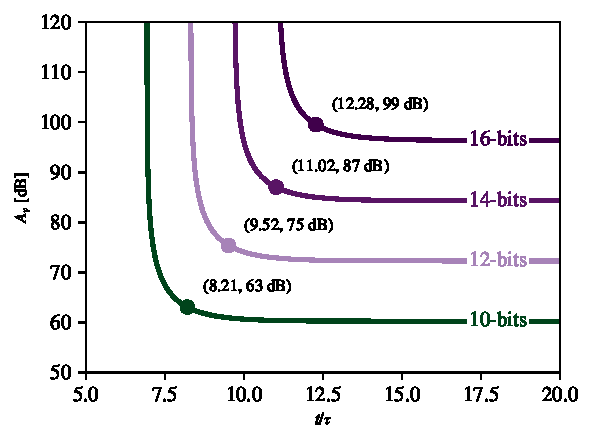
\includegraphics[width=.75\textwidth]{Chapter7/Figs/ota_spec.pdf}
    \caption{Trade-off speed versus gain of the amplifier for the SC-Integrator of the I\(\Delta\Sigma \)}
    \label{fig:ota_spec_tradeoffs}
\end{figure}

Therefore, a 12-bits accuracy requires a gain of 75 dB and a gain-bandwidth product of 952 MHz whatsoever the load is. As discussed in the Section~\ref{sec:des_speed}, and in Section~\ref{sec:mobility} there is no optimum solution to prevent the speed of the amplifier to fall over the temperature range without an adaptive biasing. Moreover, the bandwidth limitation is general and does consider the feedback factor \(\beta \) of the configuration in which the OTA is. Let's consider the case of the first stage: the \(I\Delta\Sigma \) whose integrator output is given to the following sub-ADC\@.

The feedback factor is given to be \(C_I/(C_S+C_I) \) where \(C_I\) and \(C_S\) are the respectively the integration capacitor and the sampling capacitor. The equivalent gain-bandwidth product of the system in such configuration is the product \(\beta GBW_{OTA}\). As the feedback factor is strictly less than 1, the minimum gain-bandwidth-product of the OTA shall be greater than \(952/\beta \) MHz. For the standard design of \(C_S = C_I \), this requires a design of an OTA having a \(GBW > 1.9 \) GHz even at high temperature and a DC Gain greater than 75 dB.

As the load seen by OTA varies from one clock cycle to another, only the worst case is considered for each stage. This corresponds to a 400 fF load on the first stage OTA, and a 1 pF for the second stage amplifier loading the SAR\@.

This stringent specification implies that a calibration-free ADC over the temperature range is not feasible. Nevertheless, both the gain and GBW limitation can be corrected by the use of digital calibration as in~\cite{Sahoo2013, Bafandeh2016}.

In consequence, the expectation of the OTA is corrected downwards to save power and noise with only a sufficient DC Gain over the temperature. We, therefore, investigate the possibility to use a low-power, high-gain OTA for high-speed ADC over temperature. The GBW limitation remaining the only deficiency, a digital calibration shall correct it as well as the process mismatch of surrounding capacitors.

    \subsection{Design}                          % section 4.3.2
From the review of amplifier topology in Section~\ref{sec:amplifier-review}, the folded cascode amplifier is selected. The variation around this basis is represented in \figurename~\ref{fig:ota_cfc_buf}. To operate even at reduce supply voltage, a standard high swing current mirror for the biasing circuit is preferred. Moreover, the input is a complementary differential pair to enlarge the input swing and increase the slew rate~\cite{Olivera1999}. As the amplifier will also be used in unity gain configuration the input swing is approximately the output swing. The complementary differential pair overcomes limitations arising on a Folded Cascode in this particular situation.

\begin{figure}[htp]
    \centering
    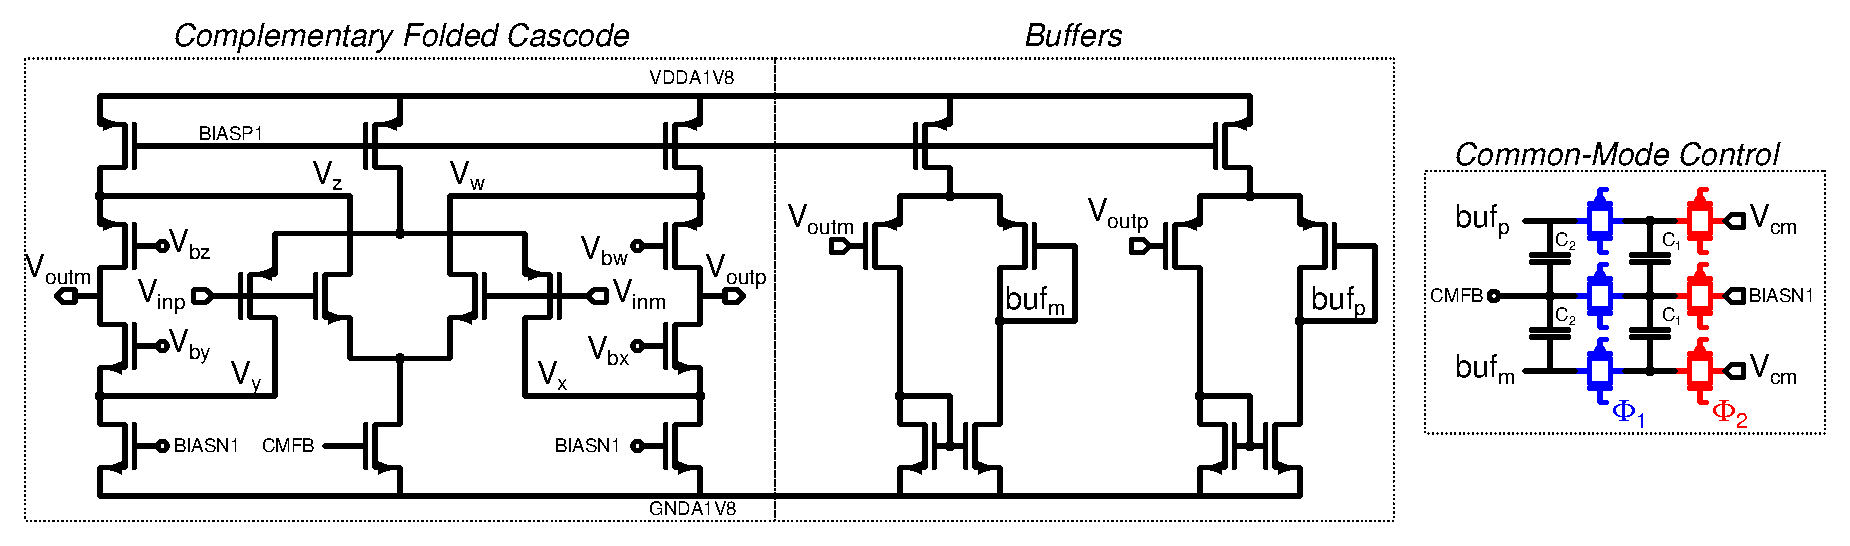
\includegraphics[width=\textwidth]{Chapter7/Figs/ota_cfc_buf_high_swing_gb}
    \caption{Designed OTA with its common-mode feedback}
    \label{fig:ota_cfc_buf}
\end{figure}

This section decomposes the amplifier design into smaller analog blocks which are: the Complementary-Folded-Cascode (CFC), the Common-Mode Control, Buffers, and Current Mirrors for the Biasing.

The CFC architecture is a modified current steering architecture that incorporates a class AB cascode stage. In this section, the design focus on one of the possible trade-offs over the temperature which lead to reduced settling time error over process and temperature variations.

Among possible trade-offs, constant current, constant gm, and constant gain are only those achievable. The Section~\ref{sec:current_density} reveals the existence of a zero temperature coefficient point for the current. Nevertheless, this point is found for a non-constant \(g_m/I_D \) ratio where both gain and transconductance suffer from the temperature variation: the slew-rate is constant over a large temperature range while the gain and speed are severely degraded. As seen in Section~\ref{sec:des_speed}, the transistor transition frequency admits no zero temperature coefficient which scales down the maximum achievable speed. The constant-gm candidate is often used in temperature aware design as it conserves the primary pole location. An extra circuit is required for the compensation of the process and voltage variation~\cite{Chu2014}. Then, the remaining option is a constant gain over temperature. This is feasible for very small current according to Section~\ref{sec:des_accuracy}.

In consequence, we propose a design where the input stage and the cascode output experience each a different design choice to blend performances.

\subsubsection{Input Differential Pairs}
While the input stage targets very high speed, the second stage should ensure a sufficient current to limit the slew rate time. As discussed earlier, we tolerate a slewing of 1 ns. This given, the slewing current should be at least 375 \(\mu \)A in the first stage and twice as much for the second stage. This current fixes for us, the biasing current.

In Section~\ref{sec:des_speed}, to achieve the maximum speed with reduced thermal dependence \(L=L_{\min} \) and a maximum current of 10\(\mu \)A for a transistor with the size of 1\(\mu \)m/180nm. For such biasing, the intrinsic gain is given to be decreasing for a temperature rising according to Section~\ref{sec:des_accuracy}. We expect then, a gain variation coming from this part of the design. But this is less relevant since most of the gain comes from the gain boosting cascode.

As the current and the transistor's length is now defined, their width is then defined by the \(g_m/I_D \) methodology. This structure has been considered in another research work and can be studied in detail in~\cite{Vallee1994,Lipka2009,Hati2012}. We keep for the design the Unity-Gain Frequency equation defined as

\begin{equation}
\omega_{ugf} = \frac{g_{m1n,m2n} + g_{m1p,m2p}}{C_L}
\end{equation}

Therefore, the sum of NMOS and PMOS transconductance should be equal to 2.5 mS in typical conditions at 27\(\degree \)C. The sizing adds an extra margin to take into account layout parasitics, process variations, and power supply variations of 10\%.

\subsubsection{Cascode Stage}
For the class AB cascode output stage, the gain, the current, and the output swing are key factors. As the current in the branch is already fixed by the slew-rate, the gain is of primary concern here.

Section~\ref{sec:des_accuracy} reveals a lessen sensitivity over temperature for 1\(\mu \)A biasing current of a referential transistor sized at 1\(\mu \)/180 nm. In order to slightly increase the gain, the cascode transistors are sized for \(L = 2 L_{\min} \).

For the current sources at the folded node, a high impedance reduces the sensitivity to the power supply variations while the capacitance shall be minimized to improve the overall speed of the OTA\@. A good trade-off has been found for \(L = 3 L_{\min} \). As the threshold voltage temperature coefficient depends on the transistor's length, as the bigger L is smaller this coefficient will be, the chosen L offers a reduced temperature sensitivity compared to \(L = L_{\min} \).

Considering an output swing from 525 mV to 1.275 V, the transistors of the cascode part cannot be in strong inversion. As their drain-source voltage is increasing with the level of inversion, the maximum output swing will be limited to \(V_{DD} - 4 V_{DS} \). As the drain-source voltage increases by 100 mV from 27\(\degree \)C to 175\(\degree \)C, a reduced power supply of \(V_{DD} - 10\% \) pushes the cascode transistors into the deep sub-threshold operating region at high temperature.

\begin{eqnarray}
    4V_{ds\max} =& (V_{GSsource,n}-V_{THsource,n}) + (V_{GScascode,n}-V_{THcascode,n}) \\
    +& (V_{GSsource,p}-V_{THsource,p}) + (V_{GScascode,p}-V_{THcascode,p}) \nonumber \\
    =& 0.9 V_{DD} - (1.275 V - 0.525 V) = 0.87 V \nonumber
\end{eqnarray}

where \(V_{GSsource}-V_{THsource} \) represents the voltage overdrive of the transistor playing the current source of the folded cascode, and \(V_{GScascode}-V_{THcascode}\) the voltage overdrive of the cascoding transistor. Let's suppose the margin split evenly across PMOS and NMOS transistors, the minimum voltage required is 0.335 V at 27\(\degree \)C for \((V_{GSsource,n}-V_{THsource,n}) + (V_{GScascode,n}-V_{THcascode,n})\).

\begin{figure}[htp]
    \centering
    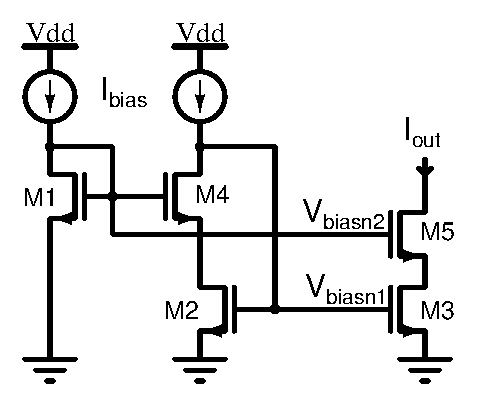
\includegraphics[width=0.5\textwidth]{Chapter7/Figs/wide-swing-current-mirror.ps}
    \caption{Wide-Swing current mirror for the biasing of the proposed OTA}
    \label{fig:wide-swing-cascode}
\end{figure}

Therefore, the wide-swing cascode biasing depicted by \figurename~\ref{fig:wide-swing-cascode} allows correct operation from an output voltage \(V_{out\min} > V_{ds3}+V_{ds5}\). \(M2 \) and \(M4 \) act like a single-diode connected transistor to create the gate source voltage for \(M3 \). Including \(M4 \) helps lower the \(V_{ds2} \) so that it matches \(V_{ds3} \). As \(V_{gs1} = V_{gs4} \), \(M2 \) and \(M3 \) are pushed at the edge of the triode region such that \(V_{ds3} = V_{ov3}\). In this operation mode, the transistors \(M2 \) and \(M3 \) are closer to the current insensitivity point with respect to the temperature defined in Section~\ref{sec:current_density}. As the transistor \(M5 \) is no more in saturation for \(V_{ds5} = V_{ov5} = V_{ov1} - V_{ov3}\), \(V_{out\min} \) shall be greater than the voltage overdrive of transistor \(M1 \). Thus the output swing is enhanced and the output resistance defined by the transistor \(M1 \).

For our application, the output swing is known and mainly defined by the voltage overdrive of one transistor for NMOS and one for PMOS\@. The design constraints are now relaxed and cascode transistors can be minimal to reduce parasitics on the output node which enhance both the speed and the PSRR frequency response~\cite{Ribner1984}.

\subsubsection{Gain Boosting}
To boost the DC gain, if appropriate, either a single-ended or a differential auxiliary amplifier can be envisioned. The single-ended boosting architecture uses four auxiliary op-amps to regulate the transconductance of cascode transistors and enhances the gain. It is first reported by \cite{Bult1990}. However, the single-ended version of the boosters is associated with some undesired effects:
\begin{itemize}
    \itemsep-0.5em
    \item[--] Signal usually travels a longer path inside the booster and sees an extra pole from an internal current mirror. Therefore, the frequency response of the booster suffers, especially when optimizing the pole-zero doublet effect.
    \item[--] Noises generated by the biasing circuitry inside the boosters are not correlated. This means the noise overhead associated with gain boosting is higher.
\end{itemize}
The problems are addressed by using a fully differential gain-boosting scheme. This improves the settling behavior and rejects the common source of noise. But fully differential amplifiers require common-mode feedback increasing the area and injecting thermal noise. A Sackinger version of the gain boosting could also be used to reduce the length of the signal path inside the booster, and to reduce the noise generated by decreasing the number of transistors needed for the amplification.

\begin{figure}[htp]
    \centering
    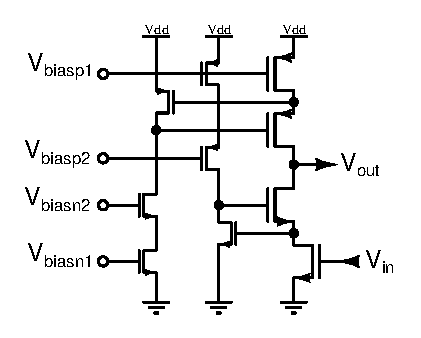
\includegraphics[width=0.5\textwidth]{Chapter7/Figs/gain-boosting.ps}
    \caption{Nested-Gain boosting for large gain OTA}
    \label{fig:nmos-nested-gain-boosting}
\end{figure}

In \figurename~\ref{fig:nmos-nested-gain-boosting}, the small size of the Sackinger version is exploited to even more enhance the DC Gain by nesting the gain boosting. This nesting requires only small size transistors which do not connect large parasitics on the folding nodes of the core amplifier. For a common source transistor, the voltage noise is given by equation (\ref{eqn:mos-noise}) which combines the thermal noise, the flicker noise, and the output resistance of the current source \(r_{Id} \).

\begin{equation}
    \label{eqn:mos-noise}
\overline{V_n^2} = \left(4k_BT\gamma g_m + \frac{K}{C_{ox}WL} \frac{g_m^2}{f} + \frac{4k_BT\Delta f}{r_{Id}}\right) {(r_o || r_{Id})}^2
\end{equation}

The noise reduction implies a large \(g_m \) coming from a transistor in strong inversion to reduce the output resistance \(r_o\). As the total noise is proportional to the output impedance of the common source configuration, the output resistance of the current source shall be large. To reduce the flicker noise, the area of the transistor shall be maximized and the transconductance minimized. Therefore an adjustment of the operation mode and the area is performed to reduce the noise spectral power. The decision is made as follows:

\begin{itemize}
    \itemsep-0.5em
    \item[--] the main gain boosting stage is designed with \(L=2L_{\min}\) and transistors operate in strong inversion to reduce the thermal noise impact.
    \item[--] nested gain boosting is designed with \(L=4L_{\min}\) and transistors operate in moderate inversion to reduce the flicker noise while giving a larger DC gain.
    \item[--] the current sources are cascoded, and regulated, to improve both the DC gain and the noise due to its output resistance.
\end{itemize}

The main gain boosting stage also impacts the settling of the overall OTA\@. For optimal settling, the speed of the gain boosting stage should respect the following criterion according to~\cite{Bult1991}

\begin{equation}
\beta \omega_{ugf} < \omega_{add} < \omega_{p2}
\end{equation}

where, \(\beta\omega_{ugf} \) is the closed-loop dominant pole frequency, \(\omega_{ugf} \) is the open-loop unity-gain frequency, \(\omega_{add} \) is the unity-gain frequency of the boosting amplifier and \(\omega_{p2} \) is the second pole frequency of the main amplifier (also the second pole of the local gain-boosting loop). In the current design, the second pole frequency of the main amplifier has been overlooked over temperature and process. This procedure has been applied then on a PMOS version of the gain boosting for the Complementary Folded Cascode.

\subsubsection{Common-Mode Control}
To regulate the common mode voltage of differential circuits, one could either use feed-forward compensation (CMFF) or feedback compensation (CMFB). The feedback compensation being more reliable than the feed-forward, the latter is disregarded.

CMFB’s stabilize common-mode voltages for differential-mode analog systems by means of adjusting the common-mode output currents. The two differential output voltages are averaged to estimate the common-mode voltage, which is compared with the designated reference of the common-mode. The difference is then amplified and converted into the common-mode output current to adjust the common-mode voltage. Most of the currently used common-mode feedback circuits fall into the following four categories:

\begin{itemize}
    \itemsep-0.5em
    \item[--] Shunt Inverters CMFB
    \item[--] Resistor-Averaged CMFB (RA-CMFB)
    \item[--] Differential Difference Amplifier CMFB (DDA-CMFB)
    \item[--] Switched-capacitor CMFB (SC-CMFB)
\end{itemize}

Whatsoever the realization is, some rules have to be fulfilled when designing a good CMFB circuit:

\begin{itemize}
    \itemsep-0.5em
    \item[--] First, a unity gain-bandwidth of the common-mode loop should be higher than the one of the input signal to prevent the decrease of the operational speed. Or at least equal.
    \item[--] Second, common-mode loop compensation is necessary to ensure the common-mode stability.
    \item[--] Third, a common-mode detector should have a linear characteristic.
    \item[--] Finally, the performance of the fully differential amplifier needs to be maintained when the CMFB circuit is connected.
\end{itemize}

For a high-speed purpose, one could consider a continuous time CMFB (CT-CMFB). CT-CMFB are usually designed based on one bloc for sensing the error on the common-mode voltage and one amplifier it.

Nowadays the trend is to scale down the supply voltage, shunted parallel inverters are more and more used to sense the common-mode voltage. There is shunted CMOS inverters as in \figurename~\ref{fig:shunt_cmos_cmfb}, but are considered not as a good practice since neither the current is well controlled nor the biasing point despite a very large output range allowed. Nevertheless, the inverter can be changed into a transistor in common source to better control the current such as in \figurename~\ref{fig:shunt_inverter_cmfb}\cite{Carillo2007,Carillo2010,Centurelli2017}. For a power supply voltage of 1.8 V, this solution turns out to be power hungry consuming more than the core itself.

\begin{figure}[htp]
    \centering
    \begin{subfigure}[b]{0.48\textwidth}
        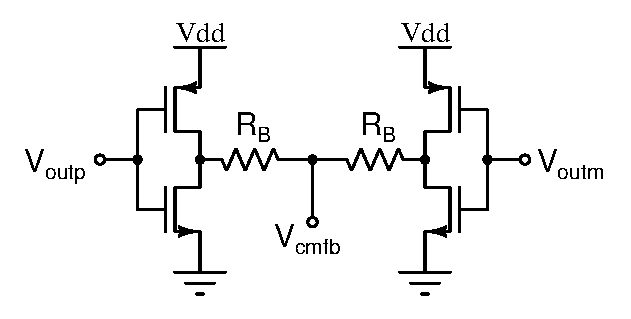
\includegraphics[width=\textwidth]{Chapter7/Figs/shunt_cmos_cmfb.ps}
        \subcaption{cmos version}
        \label{fig:shunt_cmos_cmfb}
    \end{subfigure}
    \begin{subfigure}[b]{0.48\textwidth}
        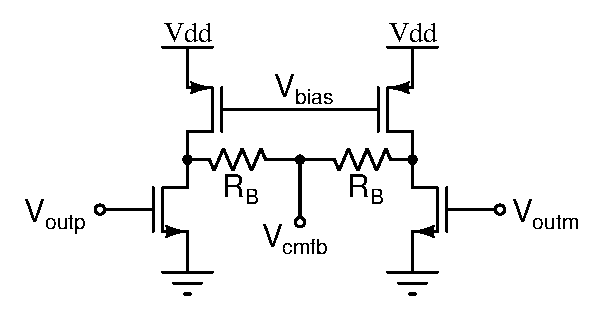
\includegraphics[width=\textwidth]{Chapter7/Figs/shunt_inverter_cmfb.ps}
        \subcaption{improved biasing}
        \label{fig:shunt_inverter_cmfb}
    \end{subfigure}
    \caption{Shunt Inverters sensing CMFB}
    \label{fig:shunt_inverter_sensing}
\end{figure}

By the way, a CMFB can be decomposed into a sensing bloc estimating the current common mode and an amplifier block to apply the correction. Assuming that the gain of the amplifier is defined by the product of an effective transconductance and the output resistance, an output resistance variation also alters the DC Gain of the amplifier, violating the fourth rule. A resistive sensing circuit as in \figurename~\ref{fig:res_sens_cmfb} thus limits the gain of the OTA and draws a current between the two outputs \(V_{outp}\) and \(V_{outm}\) through averaging resistor \(R_A \).

In order not to alter the DC Gain of the amplifier over temperature, the resistance of the common-mode sensing is replaced by two transistors in the differential pair resulting in a DDA-CMFB whose possible implementation is depicted by the \figurename~\ref{fig:dda_cmfb}. The impedance seen is therefore near infinite. As a transistor generates a current proportional to the voltage applied at its gate, DDA-CMFB becomes a relevant solution. As the power supply reduces, the DDA variant suffers from the non-linearity of the current drawn. As the temperature increase, the effect is ever more pronounced. The operating range in which the common mode voltage can be corrected is much more limited compared to the one of a switched capacitor version. In addition, the CMFB circuit shall be faster than the primary amplifier whose common mode voltage is controlled. Therefore, both the current consumption and the area are tremendously increased for high-speed high gain OTA\@.

\begin{figure}[htp]
    \centering
    \begin{subfigure}[b]{0.48\textwidth}
        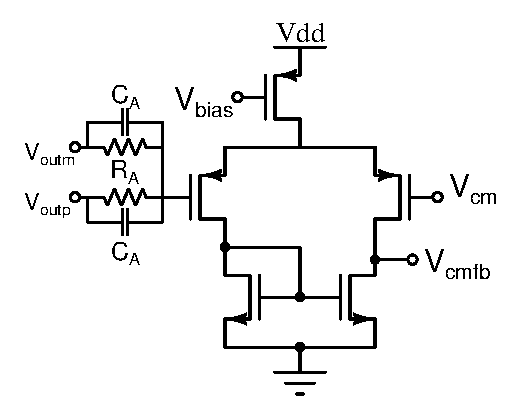
\includegraphics[height=5cm]{Chapter7/Figs/resistive_sensing_cmfb.ps}
        \subcaption{resistive sensing}
        \label{fig:res_sens_cmfb}
    \end{subfigure}
    \begin{subfigure}[b]{0.48\textwidth}
        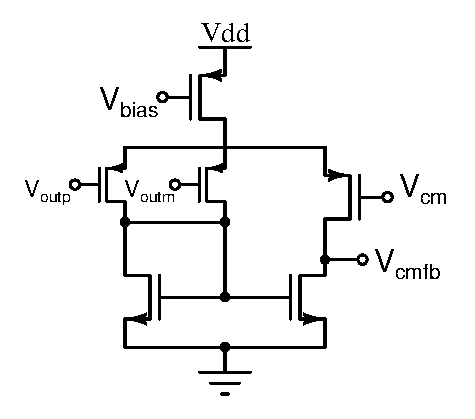
\includegraphics[height=5cm]{Chapter7/Figs/schematic_dda_cmfb.ps}
        \subcaption{DDA-CMFB}
        \label{fig:dda_cmfb}
    \end{subfigure}
    \caption{Typical continuous time CMFB}
    \label{fig:shunt_inverter_sensing}
\end{figure}

Considering an SC-CMFB, it is commonly assumed that the clock used is the same for the switched capacitor circuit surrounding the amplifier. With a standard SC-CMFB circuit as depicted by the \figurename~\ref{fig:sc-cmfb}, the size of capacitors and the sizing of switches should be determined.

\begin{figure}[htp]
    \centering
    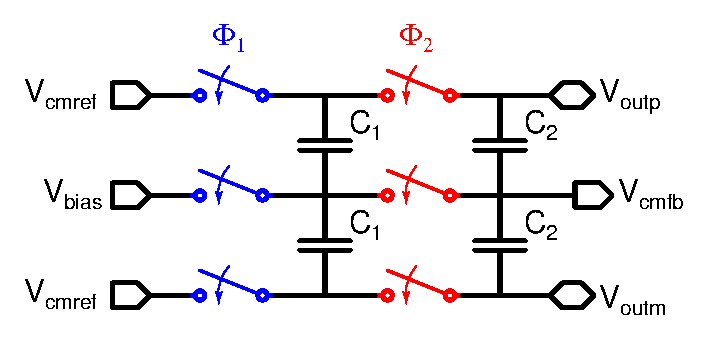
\includegraphics[width=0.5\textwidth]{Chapter7/Figs/sc-cmfb.ps}
    \caption{Standard SC CMFB circuit implemented}
    \label{fig:sc-cmfb}
\end{figure}

With respect to the DC Gain of the amplifier, the toggling of capacitor \(C_1 \) emulates a resistance connecting the output and the common mode voltage of reference. This equivalent resistance is evaluated as \(1/(C_1 F_{clk}) \) where \(F_{clk} \) is the clock frequency and \(C_1 \) the capacitor sampling \(V_{cm}-V_{BIASN1}\).

Assuming that the gain of the amplifier is defined by the product of an effective transconductance and the output resistance, the required transconductance Gm = gm-gmb = gm = 2.2 mS, a 75 dB gain results into an output resistance of 2.24 \(M\Omega \). With \(F_{clk} = 100 MHz \), the capacitance \(C_1 \) should be around 4.4 fF. A standard SC-CMFB is not feasible considering mismatch and the parasitic of switches.

Therefore, a proposition is made for the design of the CMFB circuit to blend performances. This proposition consists in using an SC-CMFB and using a voltage follower to decouple the amplifier from the switched cap circuit.
The benefits are twofold: First, the load seen by the amplifier is reduced and bumps up the unity gain frequency, and the phase margin. Second, the operating range of the CMFB circuit is enlarged compared to the DDA-CMFB circuit without reducing the gain of the amplifier.

In order to improve the accuracy of the settling voltage, the transistor's size is 220 nm/360 nm. Concerning the settling time, the ratio capacitor \(C_2/C_1 \) is crucial. From the equation (\ref{eqn:sc-cmfb}) issued in~\cite{Choksi2003}, one can intuit that the bigger the ratio is, the slower the amplifier is, and more accurate will be the settling. Considering charge injections and clock feed-through on \(C_1\), they will have a reduced impact as the ratio \(C_2/C_1\) is big and \(C_2\) capacitors driven by buffers. By the way, the gain of the cascode approximate to \(A_{cm} \) is assumed to be large to reduce the impact of biasing voltage variation. As a trade-off between settling speed and accuracy, the ratio is set to 3. This means that 3/4 of the new voltage is coming from its value at the previous clock step while 1/4 from the common-mode mismatch.

\begin{equation}
    \label{eqn:sc-cmfb}
V_{outc}[n] = \frac{C_2}{C_1+C_2} V_{outc}[n-1] + \frac{C_1}{C_1+C_2} \frac{V_{cm_{ref}}-V_{bias}}{1+\frac{1}{A_{cm}}}
\end{equation}

For the mismatch, the Pelgrom coefficient of cmm4t is 0.4 \%/\(\mu \)m. With a minimal size of 2 \(\mu \)m x 2 \(\mu \)m the mismatch coefficient of C1 is 0.14 \% and on C2 0.08 \%.

In the proposed CMFB circuit of the \figurename~\ref{fig:ota_cfc_buf}, the output buffer has 10 ns to settle accurately. The accuracy is based on the mismatch in the capacitor in the SC-CMFB circuit and the precision of the output voltage. To reduce the latter, the differential pair transistors of these buffers are sized at \(L = 3 L_{\min} \) to have a small gate capacitance and a large gain at a moderate intrinsic speed.

Buffers are not cascoded to allow a wider output swing than the core amplifier without suffering from a DC gain deficiency as they solely replicate their inputs. Then, the biasing current is 140 \(\mu \)A such that the unity gain frequency is set to be around 700 MHz. This corresponds to 7 times the speed of the clock. Therefore, most of the inaccuracy is due to the mismatch in the gain of the voltage follower set in unity gain configuration.

This buffer-sc-cmfb combination allows the design of high-gain amplifier in high frequency clocked system. This experiment is then verified over temperature and process variations.

\subsubsection{Layout Consideration}
The OTA is the core of the ADC analog and the performances of the full ADC heavily rely on the OTA\@. Therefore, the design blend constraints to reach technological limits. In the scope of the thesis, the reliability is of key concern in the design such that physical phenomenon in the manufacturing process are considered.

A folded cascode amplifier is an architecture sensitive to current mismatch at the folding node. \figurename~\ref{fig:folded-node-mismatch} represents the current error on the output node due to the mismatch. As the load is fully capacitive in most applications, the error is integrated. To minimize the error, the PMOS transistors shall be matched in that error to the ideal current value is the same. The layout will thus ensure that mechanical stress, and temperature gradient seen are the same in these PMOS transistors.

\begin{figure}[htp]
    \centering
    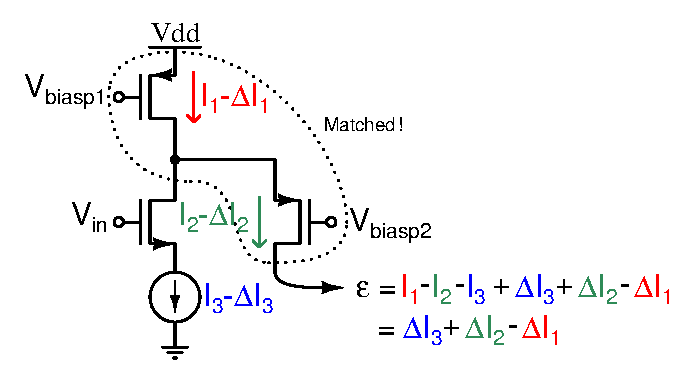
\includegraphics[width=0.6\textwidth]{Chapter7/Figs/folded-mismatch-gradient.ps}
    \caption{The error generated on the output current based on the current mismatch due to the biasing}
    \label{fig:folded-node-mismatch}
\end{figure}

The remaining source of error is thus the transistors of the differential pair generating a \textcolor{blue}{\(\Delta I_3\)} error. By design, the common mode circuit adjusts \(I_3\) to correct so that is remains only the error coming from \textcolor{red}{\(\Delta I_1\)} and \textcolor{Xgreen}{\(\Delta I_2\)} cancelling one another. Using a two differential pair (one in NMOS and one in PMOS), only the mismatch of NMOS transistors in the differential pair is compensated. As the area of PMOS differential pair is twice bigger than the area of NMOS one, \textcolor{blue}{\(\Delta I_{3p} < \Delta I_{3n}\)}.

A requirement is a good matching in current of the PMOS differential pair current source, and the NMOS-cascode of the CFC-Folded Cascode OTA which supposes a better matching in the biasing circuit.

Since the principle is applicable for both PMOS and NMOS folding nodes, the layout is split into a group of low-vth NMOS and low-vth PMOS.

To reduce \textcolor{blue}{\(\Delta I_3\)}, the layout is drawn with mechanical stress, the temperature gradient in mind with long-term viability to pay a careful attention to the current flow always in the same direction. Unfortunately, usual layout recommendation and matching analysis are typically carried out on simple rectangular transistors which become impractical for large W/L ratios of high-speed amplifiers. To be closer from test cases during matching analysis, the large differential pair is split into parallel smaller ones.

\begin{figure}[htp]
    \centering
    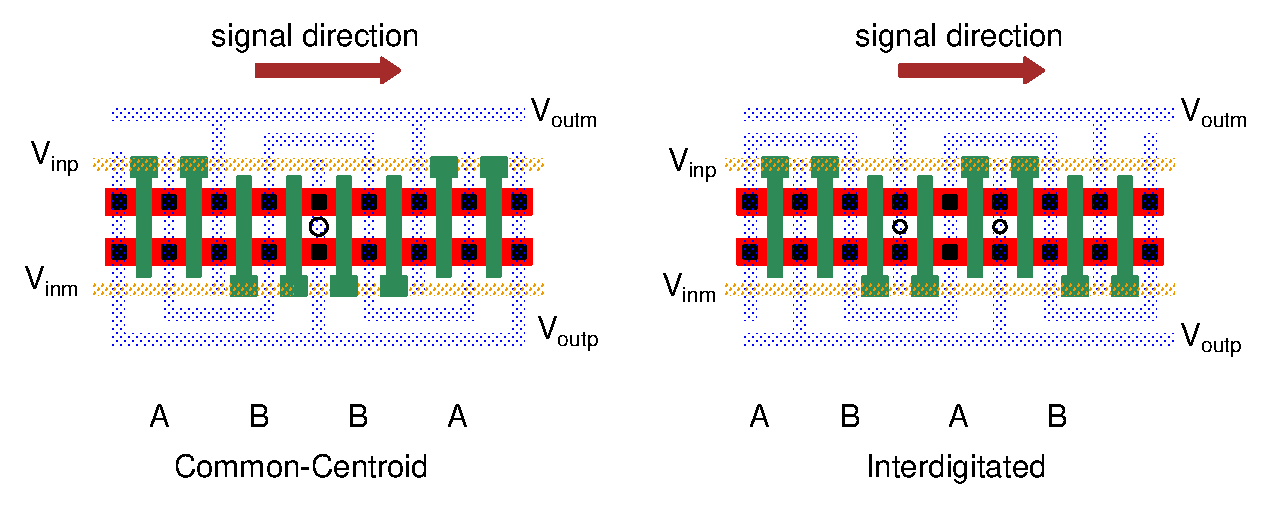
\includegraphics[width=0.85\textwidth]{Chapter7/Figs/common-centroi-vs-interdigitated.ps}
    \caption{Comparison of mismatch for common-centroid and interdigitated layout of a differential pair}
    \label{fig:common-centroid-vs-interdigitated}
\end{figure}

Among layout good matching techniques, a common centroid layout is usually the way of doing it. Suppose the gradient of stress or temperature is a linear function of the distance from the source of the stress, or from the hot spot, the average stress/temperature seen by a transistor in a differential pair is equivalent to the average stress concentrated on its centroid. As the respective centroids of the differential pair transistor are at the same position, the first order gradient is compensated. In \figurename~\ref{fig:common-centroid-vs-interdigitated}, the centroids are represented by circles for common-centroid and interdigitated layout.
The figure highlights the mismatch of centroids but also demonstrates the capacitive mismatch on the outputs.

As the transistors of the differential pair have an ever bigger W/L ratio, the differences are more pronounced. Splitting them in parallel chunks of differential pairs, with the following pattern:
\begin{vbox}
    \begin{verbatim}
 ABAB
 BABA
------
 BABA
 ABAB
    \end{verbatim}
    \vspace{-2em}
\end{vbox}
converges the centroids of A transistors and B transistors toward a common-centroid one without the capacitive mismatch on the outputs. Another advantage is a limited dispersion of transistors whose statistical mismatch is improved by a factor \(1/\sqrt{N}\) where \(N\) is the number of parallel differential pairs as given by \cite{Conti2002}.

In order to use the OTA inside a medium-to-high-resolution ADC, the OTA shall exhibit a low-noise characteristic. The traditional method to cope with the noise is at the design stage to have transistors in strong inversion with low-impedance and large parasitic capacitance to limit the bandwidth of the noise. From a layout point of view, the interdigitated transistors of the large differential pair already display such abilities. Nevertheless, an often unconsidered source of noise is the substrate coupling noise.

As power supplies of surrounding elements suffer from large IR drops, the diffusion contact into the NWELL tub (resp.\ the substrate for the ground) can easily interfere. In a process with a p+ layer substrate, the phenomenon is found to be boosted by the higher conductivity of this layer. To limit the effect, the differential pairs are surrounded by a substrate guard ring connected to the potential of the transistor source. Then, either a large space shall be allocated in the layout to increase the impedance of the coupling path or a deep trench isolation (DTI) can be used as represented in \figurename~\ref{fig:layout_noise_substrate_coupling}. As the technology allows DTI and this technique reduces the spacing needed, a ring of DTI surrounds the sensitive differential pair. This way, the noise sensitive part has been isolated from a potential noise source.

\begin{figure}[htp]
    \centering
    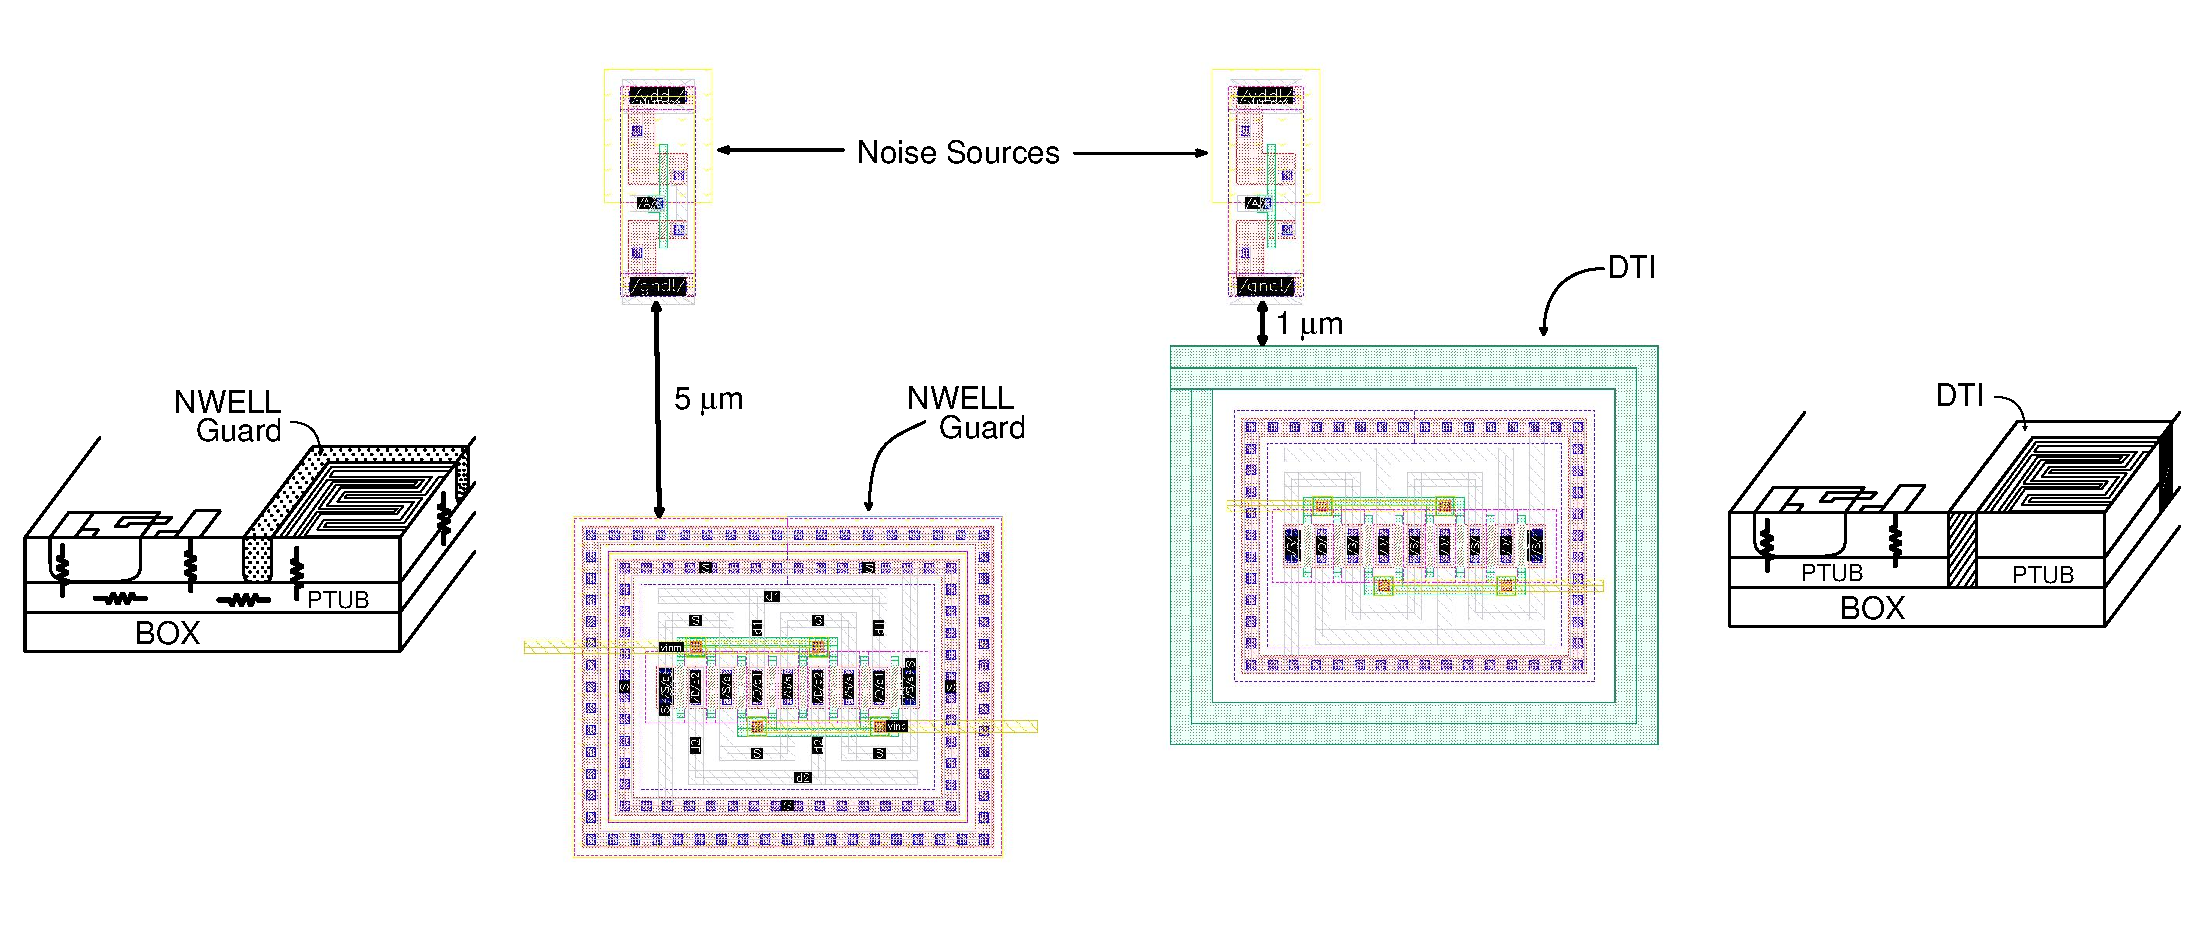
\includegraphics[width=\textwidth]{Chapter7/Figs/layout_noise_substrate.ps}
    \begin{subfigure}[b]{0.48\textwidth}
        \subcaption{NWELL guard ring}
    \end{subfigure}
    \begin{subfigure}[b]{0.48\textwidth}
        \subcaption{DTI guard ring}
    \end{subfigure}
    \caption{Substrate noise coupling with a protection based on a) a NWELL guard ring and on b) a DTI one}
    \label{fig:layout_noise_substrate_coupling}
\end{figure}

Concerning other parts, there is only one ground connection for the positive and negative branch. For a reduced impedance of the coupling path coming from the ground, a single connection point for the two branches conveys the noise in the same manner to the outputs of the OTA\@. The design being fully symmetrical and being differential, the noise from a ground coupling cancels differentially. This is not the case for the power supply coupling since each branch has a separate power supply rail. Nevertheless, the NWELL tubs increase naturally the impedance of the substrate coupling path.

\begin{figure}[htp]
    \centering
    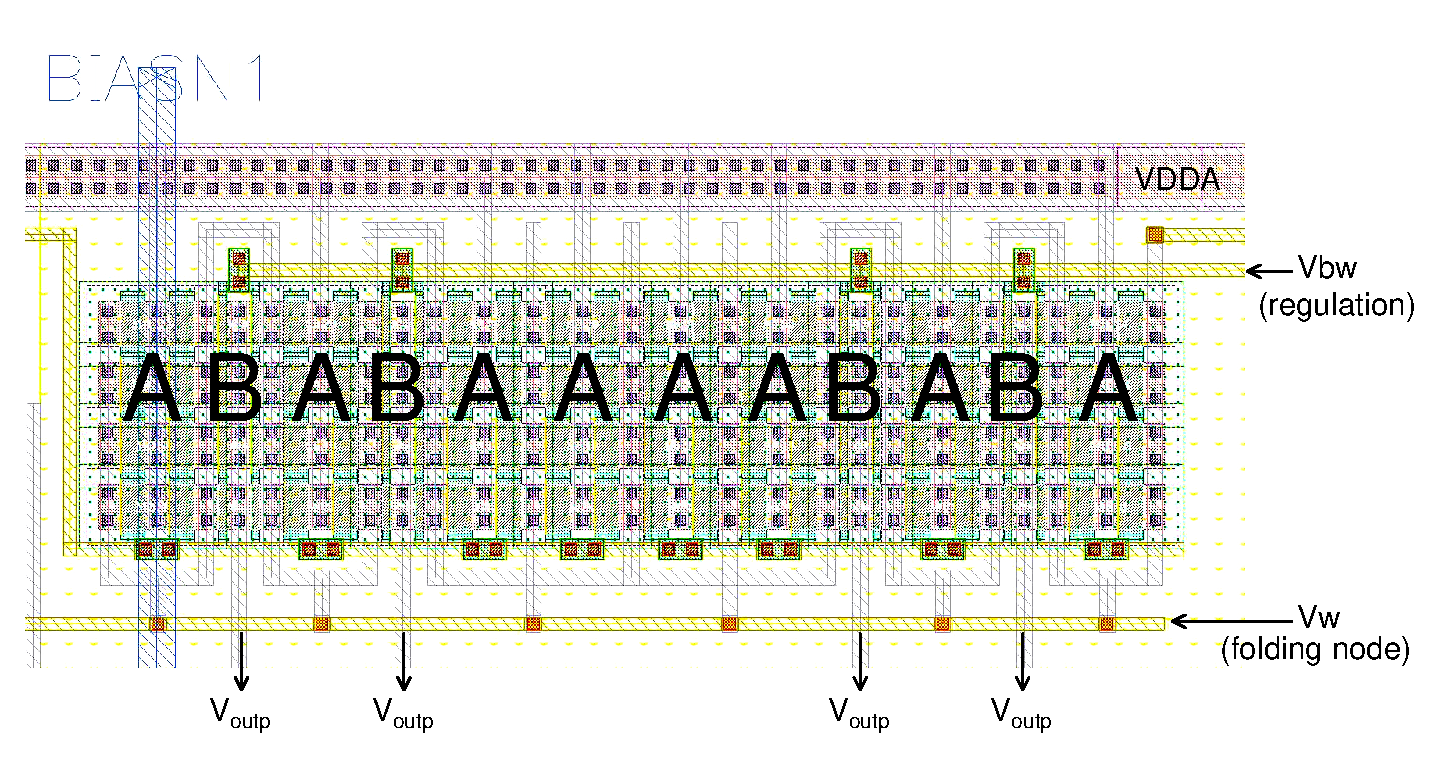
\includegraphics[width=0.75\textwidth]{Chapter7/Figs/cascode-layout-example.ps}
    \caption{Layout pattern used for the regulated cascode layout inside the same NWELL tub}
    \label{fig:layout_cascode_exemple}
\end{figure}

For the layout of the folding cascode, the L is different between the current source (A) and the cascode transistor (B). The current through A transistors is twice as much trough B transistors while the current matching even for surrounding variation shall be assured. To cope with these basic requirements the ABABAAAABABA pattern provides a common centroid for A transistors and B transistors with twice as much A than B. Moreover, both A and B are placed inside the same NWELL tub as depicted by \figurename~\ref{fig:layout_cascode_exemple}.

\begin{figure}[htp]
    \centering
    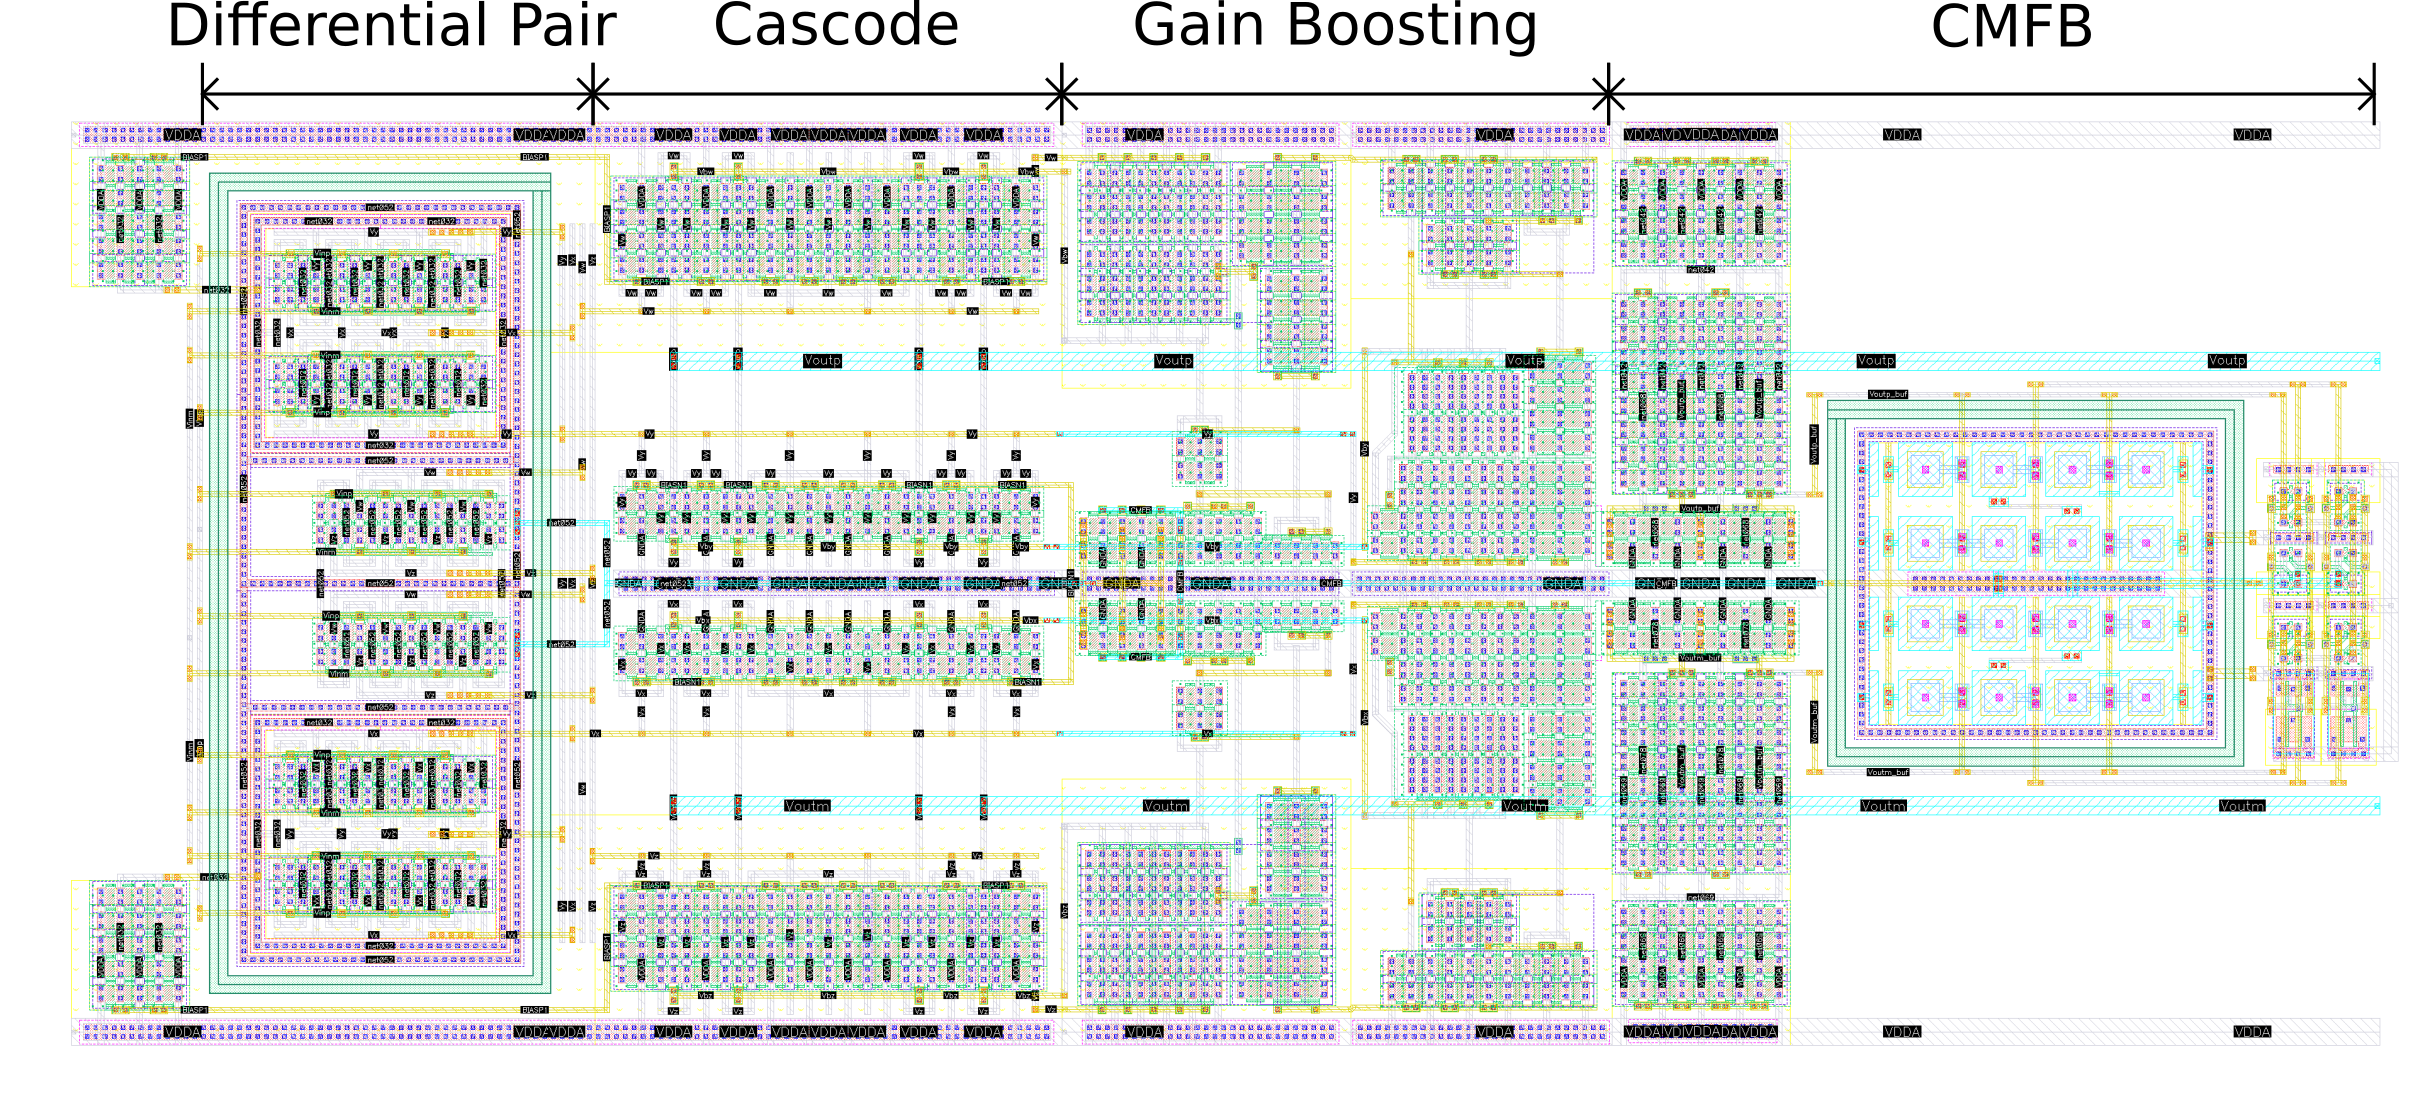
\includegraphics[width=0.85\textwidth]{Chapter7/Figs/layout_ota_v2.png}
    \caption{Gain Boosted CFC-Folded Cascode OTA layout \(52 \mu m \times 128 \mu m\)}
    \label{fig:Gain-Boosted-CFC-Folded-Cascode-OTA-layout}
\end{figure}

The weakness introduced in the current layout is the disunited layout of the biasing circuit and the OTA\@. Therefore, the matching of transistors in the biasing circuit and the OTA suffers from an extra term proportional to the distance separating them. An improvement would be to join the biasing/OTA transistor forming a current mirror in the OTA\@. In addition, the biasing voltages are propagated by METTP over the amplifier. This results in biasing voltages exposed to the surrounding of the chip and requires a reconnection for use in projects with more metal layers.

Concerning the biasing voltage of the current PMOS current sources, the cascode and the current source of the differential pair are not in common. In consequence, a mismatch is only partially corrected by the CMFB\@.

\subsection{Simulation Results}              % section 4.3.3
\label{sec:ota-sim-result}
Performance metrics of the OTA depend on its application. In our case, the metrics are the results of both small signal analysis and transient response after layout parasitic extraction:
\begin{multicols}{2}
    \begin{itemize}
        \itemsep-0.5em
        \item[--] DC Gain
        \item[--] Unity-Gain Frequency
        \item[--] Phase Margin
        \item[--] Power Consumption
        \item[--] Slew Rate
        \item[--] Settling Error
        \item[--] Noise
    \end{itemize}
\end{multicols}

\begin{figure}[htp]
    \centering
    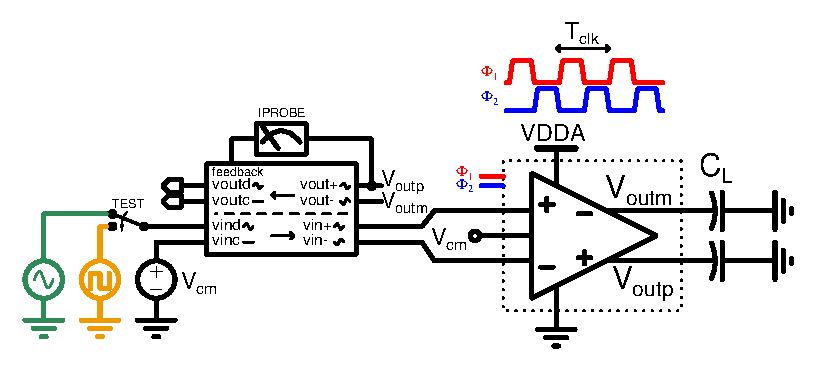
\includegraphics[width=0.75\textwidth]{Chapter7/Figs/ota_testbench.eps}
    \caption{Test bench schematic for metrics extraction}
    \label{fig:ota_testbench}
\end{figure}

For the sake of simplicity, the allotted time for the settling is defined by (\(T_{clk} - T_{nonoverlap} - T_{digital}\)) which approximates 8 ns in worst cases.

The test bench depicted by \figurename~\ref{fig:ota_testbench} sets up the OTA in a unity gain configuration, driving a capacitors \(C_L = 400 fF\) (then 1 pF) wherein the IPROBE allows one to extract the open loop AC response through a PSTB analysis (DC Gain, Unity Gain Frequency, \ldots).
\nomenclature[z]{PSTB}{Periodic STaBility}

Then, the differential input voltage is a square wave signal from \(\pm\) 500 mV around the common mode voltage of 900 mV of period 16 ns. Both the power consumption, the slew rate, and the settling error is extracted from this transient simulation. The power consumption from the current of VDDA represented in \figurename~\ref{fig:ota_settling_transient}, the slew rate as the derivative of $V_{\rm outd}$, and the settling error as the difference between $V_{\rm ind}$ and $V_{\rm outd}$ 8 ns after the transition of $V_{\rm ind}$.

\begin{figure}[htp]
    \centering
    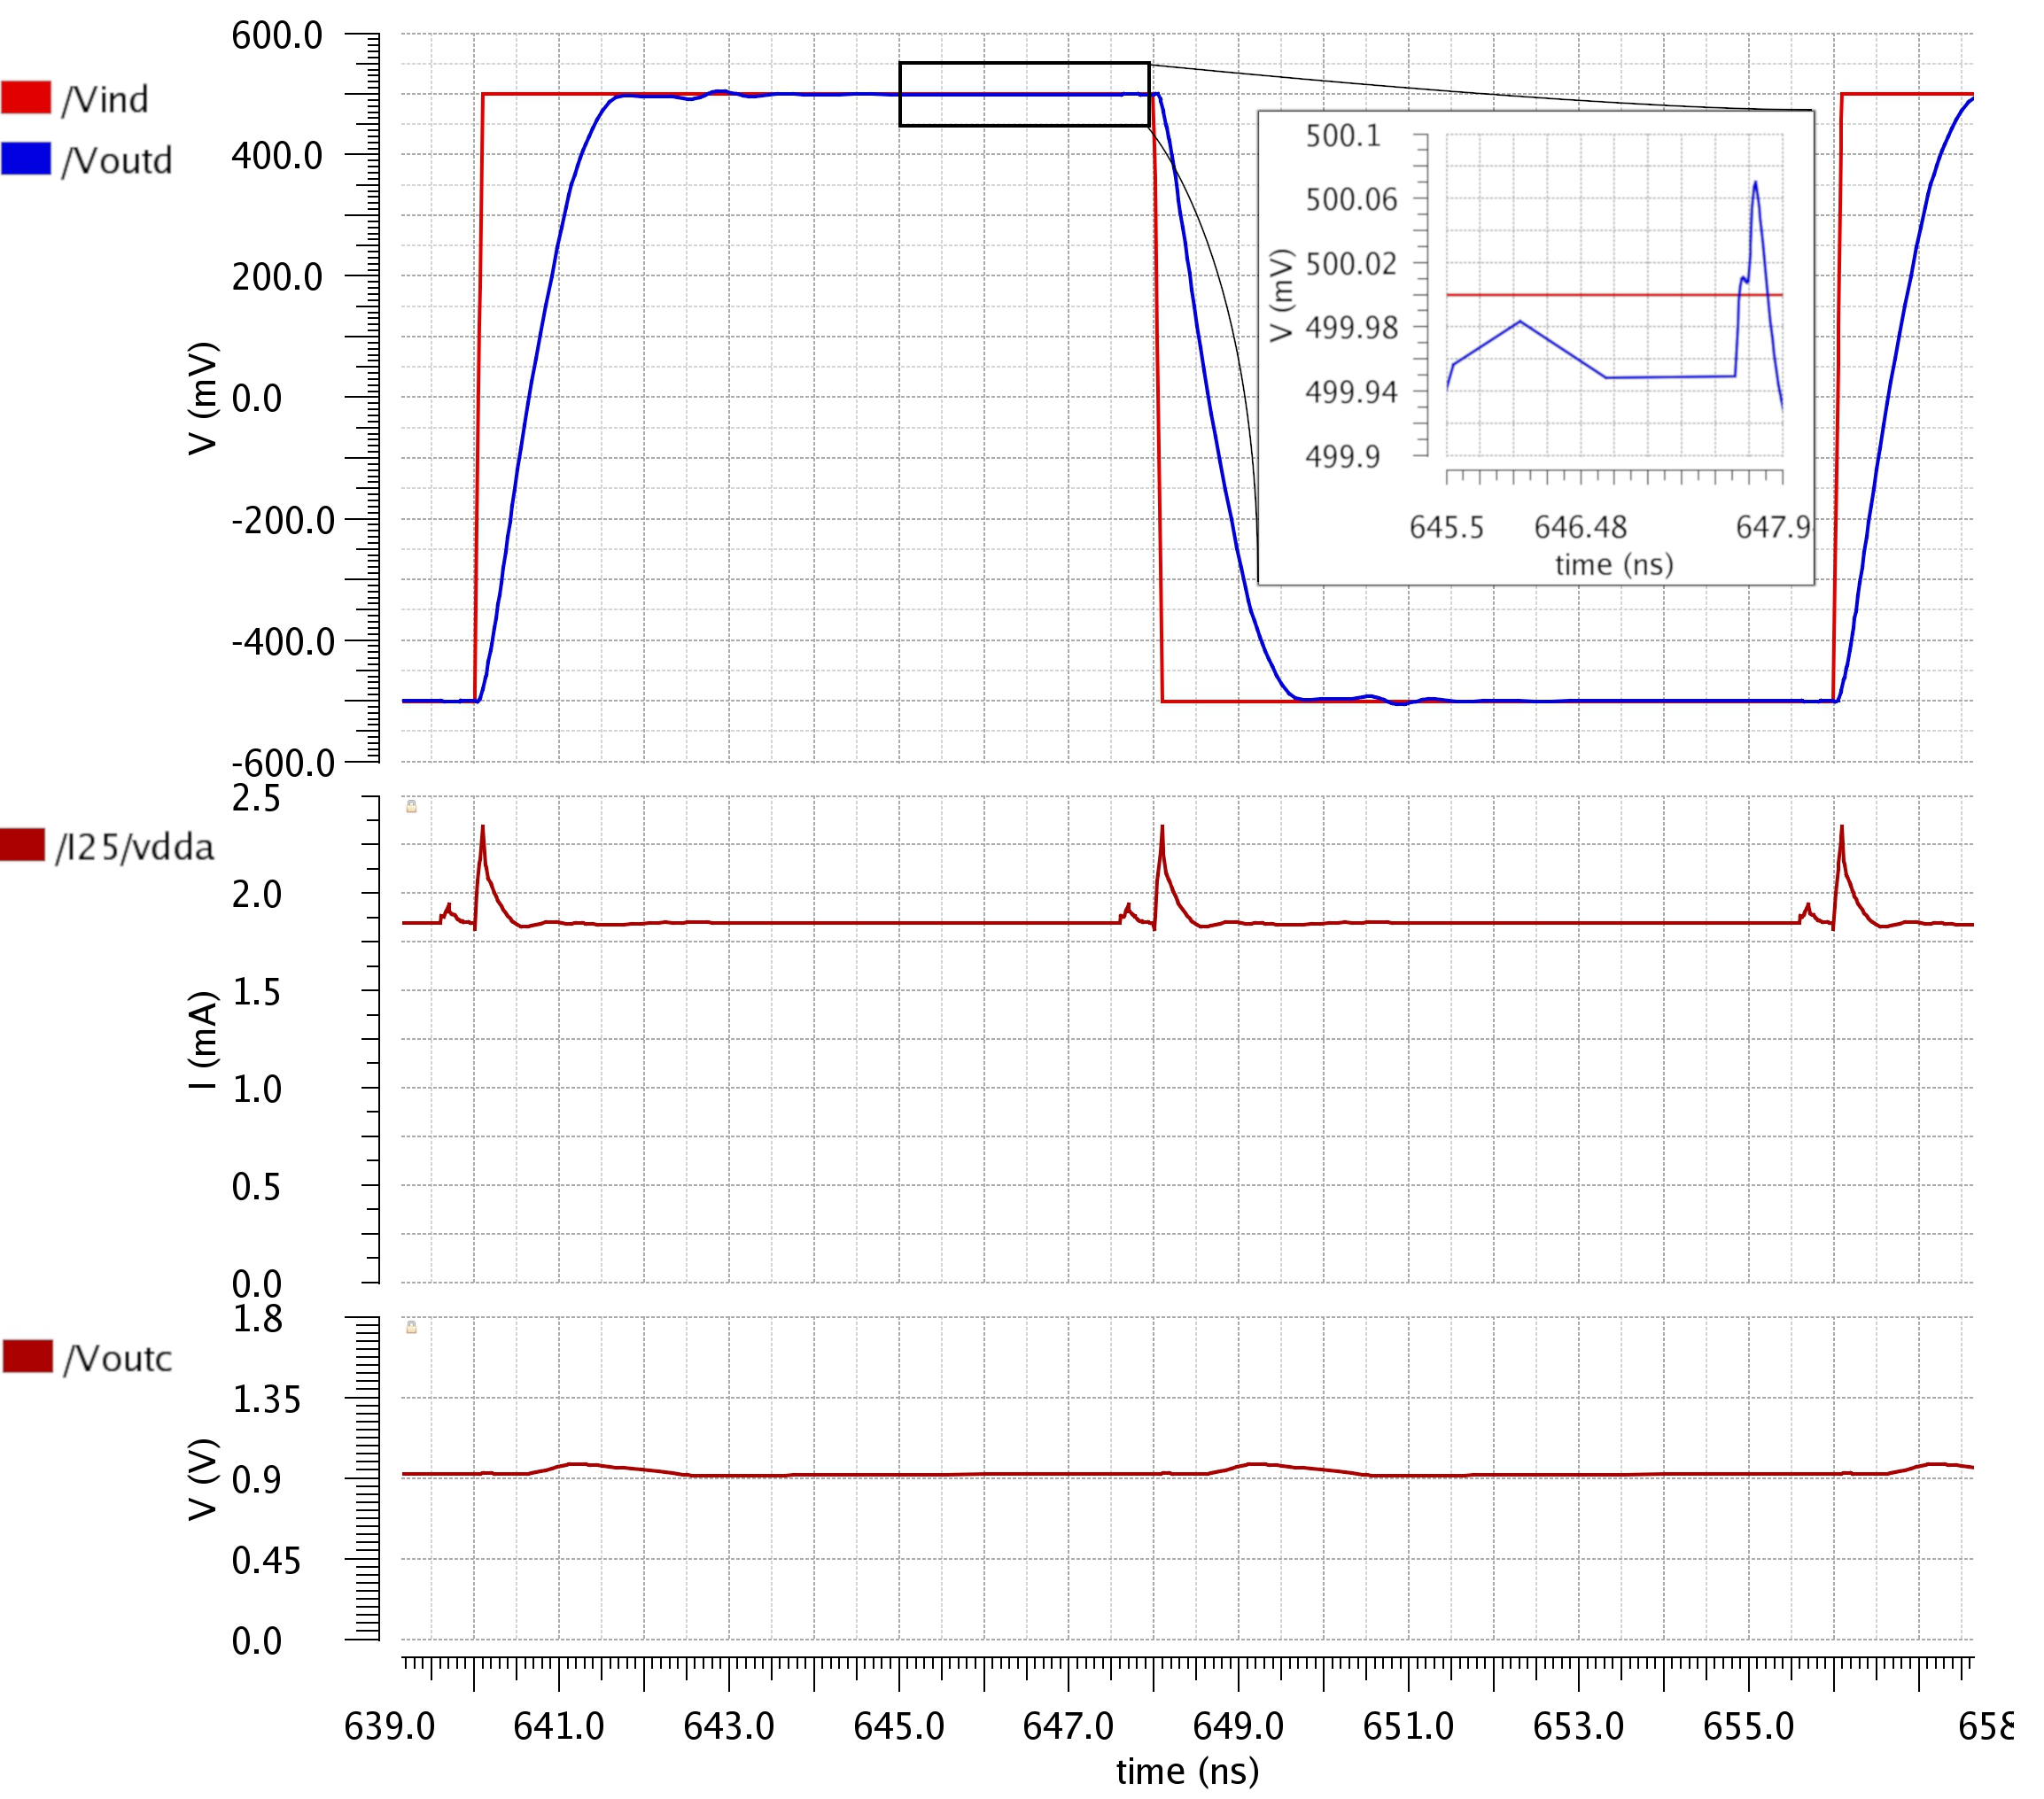
\includegraphics[width=0.75\textwidth]{Chapter7/Figs/ota_transient_settling.jpg}
    \caption{Transient waveform of the OTA in typical corner at 27$\degree$C for a power supply at 1.8 V and a load of 400 fF}
    \label{fig:ota_settling_transient}
\end{figure}

%Interactive.117 for the error
%Interactive.118 for the 70uA gain/gbw/phase margin
%Interactive.119 for the error over 1pF load

\figurename~\ref{fig:ota_result} represents variation of these metrics over temperature for different process corners. The trades made in the conception highlight a significant DC Gain, and Unity Gain Frequency drop in accordance with a biasing in moderate inversion without any compensation. This effect is more pronounced since by design the input common-mode is by 250-300 mV away from the NMOS and PMOS \(g_m \)-zero temperature coefficient (GZTC).

\begin{figure}[htp]
    \centering
    \begin{subfigure}[b]{0.48\textwidth}
        \resizebox{\textwidth}{!}{
            %% Creator: Matplotlib, PGF backend
%%
%% To include the figure in your LaTeX document, write
%%   \input{<filename>.pgf}
%%
%% Make sure the required packages are loaded in your preamble
%%   \usepackage{pgf}
%%
%% Figures using additional raster images can only be included by \input if
%% they are in the same directory as the main LaTeX file. For loading figures
%% from other directories you can use the `import` package
%%   \usepackage{import}
%% and then include the figures with
%%   \import{<path to file>}{<filename>.pgf}
%%
%% Matplotlib used the following preamble
%%   \usepackage{gensymb}
%%   \usepackage[utf8x]{inputenc}
%%   \usepackage[T1]{fontenc}
%%
\begingroup%
\makeatletter%
\begin{pgfpicture}%
\pgfpathrectangle{\pgfpointorigin}{\pgfqpoint{5.059147in}{2.855736in}}%
\pgfusepath{use as bounding box, clip}%
\begin{pgfscope}%
\pgfsetbuttcap%
\pgfsetmiterjoin%
\definecolor{currentfill}{rgb}{1.000000,1.000000,1.000000}%
\pgfsetfillcolor{currentfill}%
\pgfsetlinewidth{0.000000pt}%
\definecolor{currentstroke}{rgb}{1.000000,1.000000,1.000000}%
\pgfsetstrokecolor{currentstroke}%
\pgfsetdash{}{0pt}%
\pgfpathmoveto{\pgfqpoint{0.000000in}{0.000000in}}%
\pgfpathlineto{\pgfqpoint{5.059147in}{0.000000in}}%
\pgfpathlineto{\pgfqpoint{5.059147in}{2.855736in}}%
\pgfpathlineto{\pgfqpoint{0.000000in}{2.855736in}}%
\pgfpathclose%
\pgfusepath{fill}%
\end{pgfscope}%
\begin{pgfscope}%
\pgfsetbuttcap%
\pgfsetmiterjoin%
\definecolor{currentfill}{rgb}{1.000000,1.000000,1.000000}%
\pgfsetfillcolor{currentfill}%
\pgfsetlinewidth{0.000000pt}%
\definecolor{currentstroke}{rgb}{0.000000,0.000000,0.000000}%
\pgfsetstrokecolor{currentstroke}%
\pgfsetstrokeopacity{0.000000}%
\pgfsetdash{}{0pt}%
\pgfpathmoveto{\pgfqpoint{0.639540in}{0.631350in}}%
\pgfpathlineto{\pgfqpoint{3.722267in}{0.631350in}}%
\pgfpathlineto{\pgfqpoint{3.722267in}{2.738236in}}%
\pgfpathlineto{\pgfqpoint{0.639540in}{2.738236in}}%
\pgfpathclose%
\pgfusepath{fill}%
\end{pgfscope}%
\begin{pgfscope}%
\pgfsetbuttcap%
\pgfsetroundjoin%
\definecolor{currentfill}{rgb}{0.000000,0.000000,0.000000}%
\pgfsetfillcolor{currentfill}%
\pgfsetlinewidth{0.803000pt}%
\definecolor{currentstroke}{rgb}{0.000000,0.000000,0.000000}%
\pgfsetstrokecolor{currentstroke}%
\pgfsetdash{}{0pt}%
\pgfsys@defobject{currentmarker}{\pgfqpoint{0.000000in}{-0.048611in}}{\pgfqpoint{0.000000in}{0.000000in}}{%
\pgfpathmoveto{\pgfqpoint{0.000000in}{0.000000in}}%
\pgfpathlineto{\pgfqpoint{0.000000in}{-0.048611in}}%
\pgfusepath{stroke,fill}%
}%
\begin{pgfscope}%
\pgfsys@transformshift{0.779664in}{0.631350in}%
\pgfsys@useobject{currentmarker}{}%
\end{pgfscope}%
\end{pgfscope}%
\begin{pgfscope}%
\pgftext[x=0.779664in,y=0.534128in,,top]{\fontsize{16.000000}{19.200000}\selectfont \(\displaystyle -40\)}%
\end{pgfscope}%
\begin{pgfscope}%
\pgfsetbuttcap%
\pgfsetroundjoin%
\definecolor{currentfill}{rgb}{0.000000,0.000000,0.000000}%
\pgfsetfillcolor{currentfill}%
\pgfsetlinewidth{0.803000pt}%
\definecolor{currentstroke}{rgb}{0.000000,0.000000,0.000000}%
\pgfsetstrokecolor{currentstroke}%
\pgfsetdash{}{0pt}%
\pgfsys@defobject{currentmarker}{\pgfqpoint{0.000000in}{-0.048611in}}{\pgfqpoint{0.000000in}{0.000000in}}{%
\pgfpathmoveto{\pgfqpoint{0.000000in}{0.000000in}}%
\pgfpathlineto{\pgfqpoint{0.000000in}{-0.048611in}}%
\pgfusepath{stroke,fill}%
}%
\begin{pgfscope}%
\pgfsys@transformshift{1.301056in}{0.631350in}%
\pgfsys@useobject{currentmarker}{}%
\end{pgfscope}%
\end{pgfscope}%
\begin{pgfscope}%
\pgftext[x=1.301056in,y=0.534128in,,top]{\fontsize{16.000000}{19.200000}\selectfont \(\displaystyle 0\)}%
\end{pgfscope}%
\begin{pgfscope}%
\pgfsetbuttcap%
\pgfsetroundjoin%
\definecolor{currentfill}{rgb}{0.000000,0.000000,0.000000}%
\pgfsetfillcolor{currentfill}%
\pgfsetlinewidth{0.803000pt}%
\definecolor{currentstroke}{rgb}{0.000000,0.000000,0.000000}%
\pgfsetstrokecolor{currentstroke}%
\pgfsetdash{}{0pt}%
\pgfsys@defobject{currentmarker}{\pgfqpoint{0.000000in}{-0.048611in}}{\pgfqpoint{0.000000in}{0.000000in}}{%
\pgfpathmoveto{\pgfqpoint{0.000000in}{0.000000in}}%
\pgfpathlineto{\pgfqpoint{0.000000in}{-0.048611in}}%
\pgfusepath{stroke,fill}%
}%
\begin{pgfscope}%
\pgfsys@transformshift{1.652995in}{0.631350in}%
\pgfsys@useobject{currentmarker}{}%
\end{pgfscope}%
\end{pgfscope}%
\begin{pgfscope}%
\pgftext[x=1.652995in,y=0.534128in,,top]{\fontsize{16.000000}{19.200000}\selectfont \(\displaystyle 27\)}%
\end{pgfscope}%
\begin{pgfscope}%
\pgfsetbuttcap%
\pgfsetroundjoin%
\definecolor{currentfill}{rgb}{0.000000,0.000000,0.000000}%
\pgfsetfillcolor{currentfill}%
\pgfsetlinewidth{0.803000pt}%
\definecolor{currentstroke}{rgb}{0.000000,0.000000,0.000000}%
\pgfsetstrokecolor{currentstroke}%
\pgfsetdash{}{0pt}%
\pgfsys@defobject{currentmarker}{\pgfqpoint{0.000000in}{-0.048611in}}{\pgfqpoint{0.000000in}{0.000000in}}{%
\pgfpathmoveto{\pgfqpoint{0.000000in}{0.000000in}}%
\pgfpathlineto{\pgfqpoint{0.000000in}{-0.048611in}}%
\pgfusepath{stroke,fill}%
}%
\begin{pgfscope}%
\pgfsys@transformshift{2.409012in}{0.631350in}%
\pgfsys@useobject{currentmarker}{}%
\end{pgfscope}%
\end{pgfscope}%
\begin{pgfscope}%
\pgftext[x=2.409012in,y=0.534128in,,top]{\fontsize{16.000000}{19.200000}\selectfont \(\displaystyle 85\)}%
\end{pgfscope}%
\begin{pgfscope}%
\pgfsetbuttcap%
\pgfsetroundjoin%
\definecolor{currentfill}{rgb}{0.000000,0.000000,0.000000}%
\pgfsetfillcolor{currentfill}%
\pgfsetlinewidth{0.803000pt}%
\definecolor{currentstroke}{rgb}{0.000000,0.000000,0.000000}%
\pgfsetstrokecolor{currentstroke}%
\pgfsetdash{}{0pt}%
\pgfsys@defobject{currentmarker}{\pgfqpoint{0.000000in}{-0.048611in}}{\pgfqpoint{0.000000in}{0.000000in}}{%
\pgfpathmoveto{\pgfqpoint{0.000000in}{0.000000in}}%
\pgfpathlineto{\pgfqpoint{0.000000in}{-0.048611in}}%
\pgfusepath{stroke,fill}%
}%
\begin{pgfscope}%
\pgfsys@transformshift{2.930404in}{0.631350in}%
\pgfsys@useobject{currentmarker}{}%
\end{pgfscope}%
\end{pgfscope}%
\begin{pgfscope}%
\pgftext[x=2.930404in,y=0.534128in,,top]{\fontsize{16.000000}{19.200000}\selectfont \(\displaystyle 125\)}%
\end{pgfscope}%
\begin{pgfscope}%
\pgfsetbuttcap%
\pgfsetroundjoin%
\definecolor{currentfill}{rgb}{0.000000,0.000000,0.000000}%
\pgfsetfillcolor{currentfill}%
\pgfsetlinewidth{0.803000pt}%
\definecolor{currentstroke}{rgb}{0.000000,0.000000,0.000000}%
\pgfsetstrokecolor{currentstroke}%
\pgfsetdash{}{0pt}%
\pgfsys@defobject{currentmarker}{\pgfqpoint{0.000000in}{-0.048611in}}{\pgfqpoint{0.000000in}{0.000000in}}{%
\pgfpathmoveto{\pgfqpoint{0.000000in}{0.000000in}}%
\pgfpathlineto{\pgfqpoint{0.000000in}{-0.048611in}}%
\pgfusepath{stroke,fill}%
}%
\begin{pgfscope}%
\pgfsys@transformshift{3.582143in}{0.631350in}%
\pgfsys@useobject{currentmarker}{}%
\end{pgfscope}%
\end{pgfscope}%
\begin{pgfscope}%
\pgftext[x=3.582143in,y=0.534128in,,top]{\fontsize{16.000000}{19.200000}\selectfont \(\displaystyle 175\)}%
\end{pgfscope}%
\begin{pgfscope}%
\pgftext[x=2.180904in,y=0.266626in,,top]{\fontsize{12.000000}{14.400000}\selectfont Temperature [\(\displaystyle \degree\)C]}%
\end{pgfscope}%
\begin{pgfscope}%
\pgfsetbuttcap%
\pgfsetroundjoin%
\definecolor{currentfill}{rgb}{0.000000,0.000000,0.000000}%
\pgfsetfillcolor{currentfill}%
\pgfsetlinewidth{0.803000pt}%
\definecolor{currentstroke}{rgb}{0.000000,0.000000,0.000000}%
\pgfsetstrokecolor{currentstroke}%
\pgfsetdash{}{0pt}%
\pgfsys@defobject{currentmarker}{\pgfqpoint{-0.048611in}{0.000000in}}{\pgfqpoint{0.000000in}{0.000000in}}{%
\pgfpathmoveto{\pgfqpoint{0.000000in}{0.000000in}}%
\pgfpathlineto{\pgfqpoint{-0.048611in}{0.000000in}}%
\pgfusepath{stroke,fill}%
}%
\begin{pgfscope}%
\pgfsys@transformshift{0.639540in}{0.657760in}%
\pgfsys@useobject{currentmarker}{}%
\end{pgfscope}%
\end{pgfscope}%
\begin{pgfscope}%
\pgftext[x=0.322182in,y=0.575122in,left,base]{\fontsize{16.000000}{19.200000}\selectfont \(\displaystyle 70\)}%
\end{pgfscope}%
\begin{pgfscope}%
\pgfsetbuttcap%
\pgfsetroundjoin%
\definecolor{currentfill}{rgb}{0.000000,0.000000,0.000000}%
\pgfsetfillcolor{currentfill}%
\pgfsetlinewidth{0.803000pt}%
\definecolor{currentstroke}{rgb}{0.000000,0.000000,0.000000}%
\pgfsetstrokecolor{currentstroke}%
\pgfsetdash{}{0pt}%
\pgfsys@defobject{currentmarker}{\pgfqpoint{-0.048611in}{0.000000in}}{\pgfqpoint{0.000000in}{0.000000in}}{%
\pgfpathmoveto{\pgfqpoint{0.000000in}{0.000000in}}%
\pgfpathlineto{\pgfqpoint{-0.048611in}{0.000000in}}%
\pgfusepath{stroke,fill}%
}%
\begin{pgfscope}%
\pgfsys@transformshift{0.639540in}{1.478566in}%
\pgfsys@useobject{currentmarker}{}%
\end{pgfscope}%
\end{pgfscope}%
\begin{pgfscope}%
\pgftext[x=0.322182in,y=1.395928in,left,base]{\fontsize{16.000000}{19.200000}\selectfont \(\displaystyle 80\)}%
\end{pgfscope}%
\begin{pgfscope}%
\pgfsetbuttcap%
\pgfsetroundjoin%
\definecolor{currentfill}{rgb}{0.000000,0.000000,0.000000}%
\pgfsetfillcolor{currentfill}%
\pgfsetlinewidth{0.803000pt}%
\definecolor{currentstroke}{rgb}{0.000000,0.000000,0.000000}%
\pgfsetstrokecolor{currentstroke}%
\pgfsetdash{}{0pt}%
\pgfsys@defobject{currentmarker}{\pgfqpoint{-0.048611in}{0.000000in}}{\pgfqpoint{0.000000in}{0.000000in}}{%
\pgfpathmoveto{\pgfqpoint{0.000000in}{0.000000in}}%
\pgfpathlineto{\pgfqpoint{-0.048611in}{0.000000in}}%
\pgfusepath{stroke,fill}%
}%
\begin{pgfscope}%
\pgfsys@transformshift{0.639540in}{2.299372in}%
\pgfsys@useobject{currentmarker}{}%
\end{pgfscope}%
\end{pgfscope}%
\begin{pgfscope}%
\pgftext[x=0.322182in,y=2.216734in,left,base]{\fontsize{16.000000}{19.200000}\selectfont \(\displaystyle 90\)}%
\end{pgfscope}%
\begin{pgfscope}%
\pgftext[x=0.266626in,y=1.684793in,,bottom,rotate=90.000000]{\fontsize{12.000000}{14.400000}\selectfont DC Gain [dB]}%
\end{pgfscope}%
\begin{pgfscope}%
\pgfpathrectangle{\pgfqpoint{0.639540in}{0.631350in}}{\pgfqpoint{3.082727in}{2.106886in}} %
\pgfusepath{clip}%
\pgfsetrectcap%
\pgfsetroundjoin%
\pgfsetlinewidth{2.007500pt}%
\definecolor{currentstroke}{rgb}{0.666667,0.223529,0.223529}%
\pgfsetstrokecolor{currentstroke}%
\pgfsetdash{}{0pt}%
\pgfpathmoveto{\pgfqpoint{0.779664in}{2.097453in}}%
\pgfpathlineto{\pgfqpoint{0.966453in}{1.945194in}}%
\pgfpathlineto{\pgfqpoint{1.153371in}{1.841772in}}%
\pgfpathlineto{\pgfqpoint{1.340160in}{1.770362in}}%
\pgfpathlineto{\pgfqpoint{1.526948in}{1.719472in}}%
\pgfpathlineto{\pgfqpoint{1.713867in}{1.681305in}}%
\pgfpathlineto{\pgfqpoint{1.900656in}{1.650114in}}%
\pgfpathlineto{\pgfqpoint{2.087444in}{1.623027in}}%
\pgfpathlineto{\pgfqpoint{2.274363in}{1.596762in}}%
\pgfpathlineto{\pgfqpoint{2.461151in}{1.570496in}}%
\pgfpathlineto{\pgfqpoint{2.647549in}{1.541768in}}%
\pgfpathlineto{\pgfqpoint{2.835250in}{1.507294in}}%
\pgfpathlineto{\pgfqpoint{3.021647in}{1.460918in}}%
\pgfpathlineto{\pgfqpoint{3.208045in}{1.387867in}}%
\pgfpathlineto{\pgfqpoint{3.395746in}{1.307428in}}%
\pgfpathlineto{\pgfqpoint{3.582143in}{1.235607in}}%
\pgfusepath{stroke}%
\end{pgfscope}%
\begin{pgfscope}%
\pgfpathrectangle{\pgfqpoint{0.639540in}{0.631350in}}{\pgfqpoint{3.082727in}{2.106886in}} %
\pgfusepath{clip}%
\pgfsetrectcap%
\pgfsetroundjoin%
\pgfsetlinewidth{2.007500pt}%
\definecolor{currentstroke}{rgb}{0.666667,0.592157,0.223529}%
\pgfsetstrokecolor{currentstroke}%
\pgfsetdash{}{0pt}%
\pgfpathmoveto{\pgfqpoint{0.779664in}{2.615382in}}%
\pgfpathlineto{\pgfqpoint{0.966453in}{2.635697in}}%
\pgfpathlineto{\pgfqpoint{1.153371in}{2.642468in}}%
\pgfpathlineto{\pgfqpoint{1.340160in}{2.599786in}}%
\pgfpathlineto{\pgfqpoint{1.526948in}{2.481180in}}%
\pgfpathlineto{\pgfqpoint{1.713867in}{2.321328in}}%
\pgfpathlineto{\pgfqpoint{1.900656in}{2.170300in}}%
\pgfpathlineto{\pgfqpoint{2.087444in}{2.045332in}}%
\pgfpathlineto{\pgfqpoint{2.274363in}{1.944373in}}%
\pgfpathlineto{\pgfqpoint{2.461151in}{1.862703in}}%
\pgfpathlineto{\pgfqpoint{2.647549in}{1.794165in}}%
\pgfpathlineto{\pgfqpoint{2.835250in}{1.733631in}}%
\pgfpathlineto{\pgfqpoint{3.021647in}{1.672276in}}%
\pgfpathlineto{\pgfqpoint{3.208045in}{1.563724in}}%
\pgfpathlineto{\pgfqpoint{3.395746in}{1.463791in}}%
\pgfpathlineto{\pgfqpoint{3.582143in}{1.413312in}}%
\pgfusepath{stroke}%
\end{pgfscope}%
\begin{pgfscope}%
\pgfpathrectangle{\pgfqpoint{0.639540in}{0.631350in}}{\pgfqpoint{3.082727in}{2.106886in}} %
\pgfusepath{clip}%
\pgfsetrectcap%
\pgfsetroundjoin%
\pgfsetlinewidth{2.007500pt}%
\definecolor{currentstroke}{rgb}{0.250980,0.188235,0.458824}%
\pgfsetstrokecolor{currentstroke}%
\pgfsetdash{}{0pt}%
\pgfpathmoveto{\pgfqpoint{0.779664in}{1.645189in}}%
\pgfpathlineto{\pgfqpoint{0.966453in}{1.615640in}}%
\pgfpathlineto{\pgfqpoint{1.153371in}{1.593273in}}%
\pgfpathlineto{\pgfqpoint{1.340160in}{1.574190in}}%
\pgfpathlineto{\pgfqpoint{1.526948in}{1.556747in}}%
\pgfpathlineto{\pgfqpoint{1.713867in}{1.539305in}}%
\pgfpathlineto{\pgfqpoint{1.900656in}{1.520427in}}%
\pgfpathlineto{\pgfqpoint{2.087444in}{1.497649in}}%
\pgfpathlineto{\pgfqpoint{2.274363in}{1.466459in}}%
\pgfpathlineto{\pgfqpoint{2.461151in}{1.411670in}}%
\pgfpathlineto{\pgfqpoint{2.647549in}{1.342107in}}%
\pgfpathlineto{\pgfqpoint{2.835250in}{1.286087in}}%
\pgfpathlineto{\pgfqpoint{3.021647in}{1.225963in}}%
\pgfpathlineto{\pgfqpoint{3.208045in}{1.152500in}}%
\pgfpathlineto{\pgfqpoint{3.395746in}{1.062007in}}%
\pgfpathlineto{\pgfqpoint{3.582143in}{0.952019in}}%
\pgfusepath{stroke}%
\end{pgfscope}%
\begin{pgfscope}%
\pgfpathrectangle{\pgfqpoint{0.639540in}{0.631350in}}{\pgfqpoint{3.082727in}{2.106886in}} %
\pgfusepath{clip}%
\pgfsetrectcap%
\pgfsetroundjoin%
\pgfsetlinewidth{2.007500pt}%
\definecolor{currentstroke}{rgb}{0.176471,0.533333,0.176471}%
\pgfsetstrokecolor{currentstroke}%
\pgfsetdash{}{0pt}%
\pgfpathmoveto{\pgfqpoint{0.779664in}{2.543766in}}%
\pgfpathlineto{\pgfqpoint{0.966453in}{2.556284in}}%
\pgfpathlineto{\pgfqpoint{1.153371in}{2.554642in}}%
\pgfpathlineto{\pgfqpoint{1.340160in}{2.510524in}}%
\pgfpathlineto{\pgfqpoint{1.526948in}{2.397253in}}%
\pgfpathlineto{\pgfqpoint{1.713867in}{2.246019in}}%
\pgfpathlineto{\pgfqpoint{1.900656in}{2.104020in}}%
\pgfpathlineto{\pgfqpoint{2.087444in}{1.986644in}}%
\pgfpathlineto{\pgfqpoint{2.274363in}{1.892457in}}%
\pgfpathlineto{\pgfqpoint{2.461151in}{1.816327in}}%
\pgfpathlineto{\pgfqpoint{2.647549in}{1.753125in}}%
\pgfpathlineto{\pgfqpoint{2.835250in}{1.698542in}}%
\pgfpathlineto{\pgfqpoint{3.021647in}{1.648678in}}%
\pgfpathlineto{\pgfqpoint{3.208045in}{1.600866in}}%
\pgfpathlineto{\pgfqpoint{3.395746in}{1.550386in}}%
\pgfpathlineto{\pgfqpoint{3.582143in}{1.493751in}}%
\pgfusepath{stroke}%
\end{pgfscope}%
\begin{pgfscope}%
\pgfpathrectangle{\pgfqpoint{0.639540in}{0.631350in}}{\pgfqpoint{3.082727in}{2.106886in}} %
\pgfusepath{clip}%
\pgfsetrectcap%
\pgfsetroundjoin%
\pgfsetlinewidth{2.007500pt}%
\definecolor{currentstroke}{rgb}{0.141176,0.419608,0.380392}%
\pgfsetstrokecolor{currentstroke}%
\pgfsetdash{}{0pt}%
\pgfpathmoveto{\pgfqpoint{0.779664in}{1.595530in}}%
\pgfpathlineto{\pgfqpoint{0.966453in}{1.572137in}}%
\pgfpathlineto{\pgfqpoint{1.153371in}{1.554490in}}%
\pgfpathlineto{\pgfqpoint{1.340160in}{1.539100in}}%
\pgfpathlineto{\pgfqpoint{1.526948in}{1.523710in}}%
\pgfpathlineto{\pgfqpoint{1.713867in}{1.506268in}}%
\pgfpathlineto{\pgfqpoint{1.900656in}{1.485542in}}%
\pgfpathlineto{\pgfqpoint{2.087444in}{1.459277in}}%
\pgfpathlineto{\pgfqpoint{2.274363in}{1.425213in}}%
\pgfpathlineto{\pgfqpoint{2.461151in}{1.380890in}}%
\pgfpathlineto{\pgfqpoint{2.647549in}{1.322612in}}%
\pgfpathlineto{\pgfqpoint{2.835250in}{1.245867in}}%
\pgfpathlineto{\pgfqpoint{3.021647in}{1.147165in}}%
\pgfpathlineto{\pgfqpoint{3.208045in}{1.025070in}}%
\pgfpathlineto{\pgfqpoint{3.395746in}{0.882455in}}%
\pgfpathlineto{\pgfqpoint{3.582143in}{0.727118in}}%
\pgfusepath{stroke}%
\end{pgfscope}%
\begin{pgfscope}%
\pgfsetrectcap%
\pgfsetmiterjoin%
\pgfsetlinewidth{0.803000pt}%
\definecolor{currentstroke}{rgb}{0.000000,0.000000,0.000000}%
\pgfsetstrokecolor{currentstroke}%
\pgfsetdash{}{0pt}%
\pgfpathmoveto{\pgfqpoint{0.639540in}{0.631350in}}%
\pgfpathlineto{\pgfqpoint{0.639540in}{2.738236in}}%
\pgfusepath{stroke}%
\end{pgfscope}%
\begin{pgfscope}%
\pgfsetrectcap%
\pgfsetmiterjoin%
\pgfsetlinewidth{0.803000pt}%
\definecolor{currentstroke}{rgb}{0.000000,0.000000,0.000000}%
\pgfsetstrokecolor{currentstroke}%
\pgfsetdash{}{0pt}%
\pgfpathmoveto{\pgfqpoint{3.722267in}{0.631350in}}%
\pgfpathlineto{\pgfqpoint{3.722267in}{2.738236in}}%
\pgfusepath{stroke}%
\end{pgfscope}%
\begin{pgfscope}%
\pgfsetrectcap%
\pgfsetmiterjoin%
\pgfsetlinewidth{0.803000pt}%
\definecolor{currentstroke}{rgb}{0.000000,0.000000,0.000000}%
\pgfsetstrokecolor{currentstroke}%
\pgfsetdash{}{0pt}%
\pgfpathmoveto{\pgfqpoint{0.639540in}{0.631350in}}%
\pgfpathlineto{\pgfqpoint{3.722267in}{0.631350in}}%
\pgfusepath{stroke}%
\end{pgfscope}%
\begin{pgfscope}%
\pgfsetrectcap%
\pgfsetmiterjoin%
\pgfsetlinewidth{0.803000pt}%
\definecolor{currentstroke}{rgb}{0.000000,0.000000,0.000000}%
\pgfsetstrokecolor{currentstroke}%
\pgfsetdash{}{0pt}%
\pgfpathmoveto{\pgfqpoint{0.639540in}{2.738236in}}%
\pgfpathlineto{\pgfqpoint{3.722267in}{2.738236in}}%
\pgfusepath{stroke}%
\end{pgfscope}%
\begin{pgfscope}%
\pgfsetbuttcap%
\pgfsetmiterjoin%
\definecolor{currentfill}{rgb}{1.000000,1.000000,1.000000}%
\pgfsetfillcolor{currentfill}%
\pgfsetfillopacity{0.800000}%
\pgfsetlinewidth{1.003750pt}%
\definecolor{currentstroke}{rgb}{0.800000,0.800000,0.800000}%
\pgfsetstrokecolor{currentstroke}%
\pgfsetstrokeopacity{0.800000}%
\pgfsetdash{}{0pt}%
\pgfpathmoveto{\pgfqpoint{3.877823in}{0.945170in}}%
\pgfpathlineto{\pgfqpoint{4.914703in}{0.945170in}}%
\pgfpathquadraticcurveto{\pgfqpoint{4.959147in}{0.945170in}}{\pgfqpoint{4.959147in}{0.989614in}}%
\pgfpathlineto{\pgfqpoint{4.959147in}{2.582680in}}%
\pgfpathquadraticcurveto{\pgfqpoint{4.959147in}{2.627125in}}{\pgfqpoint{4.914703in}{2.627125in}}%
\pgfpathlineto{\pgfqpoint{3.877823in}{2.627125in}}%
\pgfpathquadraticcurveto{\pgfqpoint{3.833378in}{2.627125in}}{\pgfqpoint{3.833378in}{2.582680in}}%
\pgfpathlineto{\pgfqpoint{3.833378in}{0.989614in}}%
\pgfpathquadraticcurveto{\pgfqpoint{3.833378in}{0.945170in}}{\pgfqpoint{3.877823in}{0.945170in}}%
\pgfpathclose%
\pgfusepath{stroke,fill}%
\end{pgfscope}%
\begin{pgfscope}%
\pgfsetrectcap%
\pgfsetroundjoin%
\pgfsetlinewidth{2.007500pt}%
\definecolor{currentstroke}{rgb}{0.666667,0.223529,0.223529}%
\pgfsetstrokecolor{currentstroke}%
\pgfsetdash{}{0pt}%
\pgfpathmoveto{\pgfqpoint{3.922267in}{2.450738in}}%
\pgfpathlineto{\pgfqpoint{4.366711in}{2.450738in}}%
\pgfusepath{stroke}%
\end{pgfscope}%
\begin{pgfscope}%
\pgftext[x=4.544489in,y=2.372960in,left,base]{\fontsize{16.000000}{19.200000}\selectfont TT}%
\end{pgfscope}%
\begin{pgfscope}%
\pgfsetrectcap%
\pgfsetroundjoin%
\pgfsetlinewidth{2.007500pt}%
\definecolor{currentstroke}{rgb}{0.666667,0.592157,0.223529}%
\pgfsetstrokecolor{currentstroke}%
\pgfsetdash{}{0pt}%
\pgfpathmoveto{\pgfqpoint{3.922267in}{2.127680in}}%
\pgfpathlineto{\pgfqpoint{4.366711in}{2.127680in}}%
\pgfusepath{stroke}%
\end{pgfscope}%
\begin{pgfscope}%
\pgftext[x=4.544489in,y=2.049902in,left,base]{\fontsize{16.000000}{19.200000}\selectfont FS}%
\end{pgfscope}%
\begin{pgfscope}%
\pgfsetrectcap%
\pgfsetroundjoin%
\pgfsetlinewidth{2.007500pt}%
\definecolor{currentstroke}{rgb}{0.250980,0.188235,0.458824}%
\pgfsetstrokecolor{currentstroke}%
\pgfsetdash{}{0pt}%
\pgfpathmoveto{\pgfqpoint{3.922267in}{1.804622in}}%
\pgfpathlineto{\pgfqpoint{4.366711in}{1.804622in}}%
\pgfusepath{stroke}%
\end{pgfscope}%
\begin{pgfscope}%
\pgftext[x=4.544489in,y=1.726845in,left,base]{\fontsize{16.000000}{19.200000}\selectfont FF}%
\end{pgfscope}%
\begin{pgfscope}%
\pgfsetrectcap%
\pgfsetroundjoin%
\pgfsetlinewidth{2.007500pt}%
\definecolor{currentstroke}{rgb}{0.176471,0.533333,0.176471}%
\pgfsetstrokecolor{currentstroke}%
\pgfsetdash{}{0pt}%
\pgfpathmoveto{\pgfqpoint{3.922267in}{1.481565in}}%
\pgfpathlineto{\pgfqpoint{4.366711in}{1.481565in}}%
\pgfusepath{stroke}%
\end{pgfscope}%
\begin{pgfscope}%
\pgftext[x=4.544489in,y=1.403787in,left,base]{\fontsize{16.000000}{19.200000}\selectfont SS}%
\end{pgfscope}%
\begin{pgfscope}%
\pgfsetrectcap%
\pgfsetroundjoin%
\pgfsetlinewidth{2.007500pt}%
\definecolor{currentstroke}{rgb}{0.141176,0.419608,0.380392}%
\pgfsetstrokecolor{currentstroke}%
\pgfsetdash{}{0pt}%
\pgfpathmoveto{\pgfqpoint{3.922267in}{1.158507in}}%
\pgfpathlineto{\pgfqpoint{4.366711in}{1.158507in}}%
\pgfusepath{stroke}%
\end{pgfscope}%
\begin{pgfscope}%
\pgftext[x=4.544489in,y=1.080729in,left,base]{\fontsize{16.000000}{19.200000}\selectfont SF}%
\end{pgfscope}%
\end{pgfpicture}%
\makeatother%
\endgroup%

        }
        \subcaption{\(3\sigma \) DC Gain}
        \label{fig:ota_dc_gain_temp_corners}
    \end{subfigure}
    \begin{subfigure}[b]{0.48\textwidth}
        \resizebox{\textwidth}{!}{
            %% Creator: Matplotlib, PGF backend
%%
%% To include the figure in your LaTeX document, write
%%   \input{<filename>.pgf}
%%
%% Make sure the required packages are loaded in your preamble
%%   \usepackage{pgf}
%%
%% Figures using additional raster images can only be included by \input if
%% they are in the same directory as the main LaTeX file. For loading figures
%% from other directories you can use the `import` package
%%   \usepackage{import}
%% and then include the figures with
%%   \import{<path to file>}{<filename>.pgf}
%%
%% Matplotlib used the following preamble
%%   \usepackage{gensymb}
%%   \usepackage[utf8x]{inputenc}
%%   \usepackage[T1]{fontenc}
%%
\begingroup%
\makeatletter%
\begin{pgfpicture}%
\pgfpathrectangle{\pgfpointorigin}{\pgfqpoint{5.059147in}{2.855736in}}%
\pgfusepath{use as bounding box, clip}%
\begin{pgfscope}%
\pgfsetbuttcap%
\pgfsetmiterjoin%
\definecolor{currentfill}{rgb}{1.000000,1.000000,1.000000}%
\pgfsetfillcolor{currentfill}%
\pgfsetlinewidth{0.000000pt}%
\definecolor{currentstroke}{rgb}{1.000000,1.000000,1.000000}%
\pgfsetstrokecolor{currentstroke}%
\pgfsetdash{}{0pt}%
\pgfpathmoveto{\pgfqpoint{0.000000in}{0.000000in}}%
\pgfpathlineto{\pgfqpoint{5.059147in}{0.000000in}}%
\pgfpathlineto{\pgfqpoint{5.059147in}{2.855736in}}%
\pgfpathlineto{\pgfqpoint{0.000000in}{2.855736in}}%
\pgfpathclose%
\pgfusepath{fill}%
\end{pgfscope}%
\begin{pgfscope}%
\pgfsetbuttcap%
\pgfsetmiterjoin%
\definecolor{currentfill}{rgb}{1.000000,1.000000,1.000000}%
\pgfsetfillcolor{currentfill}%
\pgfsetlinewidth{0.000000pt}%
\definecolor{currentstroke}{rgb}{0.000000,0.000000,0.000000}%
\pgfsetstrokecolor{currentstroke}%
\pgfsetstrokeopacity{0.000000}%
\pgfsetdash{}{0pt}%
\pgfpathmoveto{\pgfqpoint{0.639540in}{0.631350in}}%
\pgfpathlineto{\pgfqpoint{3.722267in}{0.631350in}}%
\pgfpathlineto{\pgfqpoint{3.722267in}{2.738236in}}%
\pgfpathlineto{\pgfqpoint{0.639540in}{2.738236in}}%
\pgfpathclose%
\pgfusepath{fill}%
\end{pgfscope}%
\begin{pgfscope}%
\pgfsetbuttcap%
\pgfsetroundjoin%
\definecolor{currentfill}{rgb}{0.000000,0.000000,0.000000}%
\pgfsetfillcolor{currentfill}%
\pgfsetlinewidth{0.803000pt}%
\definecolor{currentstroke}{rgb}{0.000000,0.000000,0.000000}%
\pgfsetstrokecolor{currentstroke}%
\pgfsetdash{}{0pt}%
\pgfsys@defobject{currentmarker}{\pgfqpoint{0.000000in}{-0.048611in}}{\pgfqpoint{0.000000in}{0.000000in}}{%
\pgfpathmoveto{\pgfqpoint{0.000000in}{0.000000in}}%
\pgfpathlineto{\pgfqpoint{0.000000in}{-0.048611in}}%
\pgfusepath{stroke,fill}%
}%
\begin{pgfscope}%
\pgfsys@transformshift{0.779664in}{0.631350in}%
\pgfsys@useobject{currentmarker}{}%
\end{pgfscope}%
\end{pgfscope}%
\begin{pgfscope}%
\pgftext[x=0.779664in,y=0.534128in,,top]{\fontsize{16.000000}{19.200000}\selectfont \(\displaystyle -40\)}%
\end{pgfscope}%
\begin{pgfscope}%
\pgfsetbuttcap%
\pgfsetroundjoin%
\definecolor{currentfill}{rgb}{0.000000,0.000000,0.000000}%
\pgfsetfillcolor{currentfill}%
\pgfsetlinewidth{0.803000pt}%
\definecolor{currentstroke}{rgb}{0.000000,0.000000,0.000000}%
\pgfsetstrokecolor{currentstroke}%
\pgfsetdash{}{0pt}%
\pgfsys@defobject{currentmarker}{\pgfqpoint{0.000000in}{-0.048611in}}{\pgfqpoint{0.000000in}{0.000000in}}{%
\pgfpathmoveto{\pgfqpoint{0.000000in}{0.000000in}}%
\pgfpathlineto{\pgfqpoint{0.000000in}{-0.048611in}}%
\pgfusepath{stroke,fill}%
}%
\begin{pgfscope}%
\pgfsys@transformshift{1.301056in}{0.631350in}%
\pgfsys@useobject{currentmarker}{}%
\end{pgfscope}%
\end{pgfscope}%
\begin{pgfscope}%
\pgftext[x=1.301056in,y=0.534128in,,top]{\fontsize{16.000000}{19.200000}\selectfont \(\displaystyle 0\)}%
\end{pgfscope}%
\begin{pgfscope}%
\pgfsetbuttcap%
\pgfsetroundjoin%
\definecolor{currentfill}{rgb}{0.000000,0.000000,0.000000}%
\pgfsetfillcolor{currentfill}%
\pgfsetlinewidth{0.803000pt}%
\definecolor{currentstroke}{rgb}{0.000000,0.000000,0.000000}%
\pgfsetstrokecolor{currentstroke}%
\pgfsetdash{}{0pt}%
\pgfsys@defobject{currentmarker}{\pgfqpoint{0.000000in}{-0.048611in}}{\pgfqpoint{0.000000in}{0.000000in}}{%
\pgfpathmoveto{\pgfqpoint{0.000000in}{0.000000in}}%
\pgfpathlineto{\pgfqpoint{0.000000in}{-0.048611in}}%
\pgfusepath{stroke,fill}%
}%
\begin{pgfscope}%
\pgfsys@transformshift{1.652995in}{0.631350in}%
\pgfsys@useobject{currentmarker}{}%
\end{pgfscope}%
\end{pgfscope}%
\begin{pgfscope}%
\pgftext[x=1.652995in,y=0.534128in,,top]{\fontsize{16.000000}{19.200000}\selectfont \(\displaystyle 27\)}%
\end{pgfscope}%
\begin{pgfscope}%
\pgfsetbuttcap%
\pgfsetroundjoin%
\definecolor{currentfill}{rgb}{0.000000,0.000000,0.000000}%
\pgfsetfillcolor{currentfill}%
\pgfsetlinewidth{0.803000pt}%
\definecolor{currentstroke}{rgb}{0.000000,0.000000,0.000000}%
\pgfsetstrokecolor{currentstroke}%
\pgfsetdash{}{0pt}%
\pgfsys@defobject{currentmarker}{\pgfqpoint{0.000000in}{-0.048611in}}{\pgfqpoint{0.000000in}{0.000000in}}{%
\pgfpathmoveto{\pgfqpoint{0.000000in}{0.000000in}}%
\pgfpathlineto{\pgfqpoint{0.000000in}{-0.048611in}}%
\pgfusepath{stroke,fill}%
}%
\begin{pgfscope}%
\pgfsys@transformshift{2.409012in}{0.631350in}%
\pgfsys@useobject{currentmarker}{}%
\end{pgfscope}%
\end{pgfscope}%
\begin{pgfscope}%
\pgftext[x=2.409012in,y=0.534128in,,top]{\fontsize{16.000000}{19.200000}\selectfont \(\displaystyle 85\)}%
\end{pgfscope}%
\begin{pgfscope}%
\pgfsetbuttcap%
\pgfsetroundjoin%
\definecolor{currentfill}{rgb}{0.000000,0.000000,0.000000}%
\pgfsetfillcolor{currentfill}%
\pgfsetlinewidth{0.803000pt}%
\definecolor{currentstroke}{rgb}{0.000000,0.000000,0.000000}%
\pgfsetstrokecolor{currentstroke}%
\pgfsetdash{}{0pt}%
\pgfsys@defobject{currentmarker}{\pgfqpoint{0.000000in}{-0.048611in}}{\pgfqpoint{0.000000in}{0.000000in}}{%
\pgfpathmoveto{\pgfqpoint{0.000000in}{0.000000in}}%
\pgfpathlineto{\pgfqpoint{0.000000in}{-0.048611in}}%
\pgfusepath{stroke,fill}%
}%
\begin{pgfscope}%
\pgfsys@transformshift{2.930404in}{0.631350in}%
\pgfsys@useobject{currentmarker}{}%
\end{pgfscope}%
\end{pgfscope}%
\begin{pgfscope}%
\pgftext[x=2.930404in,y=0.534128in,,top]{\fontsize{16.000000}{19.200000}\selectfont \(\displaystyle 125\)}%
\end{pgfscope}%
\begin{pgfscope}%
\pgfsetbuttcap%
\pgfsetroundjoin%
\definecolor{currentfill}{rgb}{0.000000,0.000000,0.000000}%
\pgfsetfillcolor{currentfill}%
\pgfsetlinewidth{0.803000pt}%
\definecolor{currentstroke}{rgb}{0.000000,0.000000,0.000000}%
\pgfsetstrokecolor{currentstroke}%
\pgfsetdash{}{0pt}%
\pgfsys@defobject{currentmarker}{\pgfqpoint{0.000000in}{-0.048611in}}{\pgfqpoint{0.000000in}{0.000000in}}{%
\pgfpathmoveto{\pgfqpoint{0.000000in}{0.000000in}}%
\pgfpathlineto{\pgfqpoint{0.000000in}{-0.048611in}}%
\pgfusepath{stroke,fill}%
}%
\begin{pgfscope}%
\pgfsys@transformshift{3.582143in}{0.631350in}%
\pgfsys@useobject{currentmarker}{}%
\end{pgfscope}%
\end{pgfscope}%
\begin{pgfscope}%
\pgftext[x=3.582143in,y=0.534128in,,top]{\fontsize{16.000000}{19.200000}\selectfont \(\displaystyle 175\)}%
\end{pgfscope}%
\begin{pgfscope}%
\pgftext[x=2.180904in,y=0.266626in,,top]{\fontsize{12.000000}{14.400000}\selectfont Temperature [\(\displaystyle \degree\)C]}%
\end{pgfscope}%
\begin{pgfscope}%
\pgfsetbuttcap%
\pgfsetroundjoin%
\definecolor{currentfill}{rgb}{0.000000,0.000000,0.000000}%
\pgfsetfillcolor{currentfill}%
\pgfsetlinewidth{0.803000pt}%
\definecolor{currentstroke}{rgb}{0.000000,0.000000,0.000000}%
\pgfsetstrokecolor{currentstroke}%
\pgfsetdash{}{0pt}%
\pgfsys@defobject{currentmarker}{\pgfqpoint{-0.048611in}{0.000000in}}{\pgfqpoint{0.000000in}{0.000000in}}{%
\pgfpathmoveto{\pgfqpoint{0.000000in}{0.000000in}}%
\pgfpathlineto{\pgfqpoint{-0.048611in}{0.000000in}}%
\pgfusepath{stroke,fill}%
}%
\begin{pgfscope}%
\pgfsys@transformshift{0.639540in}{1.149557in}%
\pgfsys@useobject{currentmarker}{}%
\end{pgfscope}%
\end{pgfscope}%
\begin{pgfscope}%
\pgftext[x=0.322182in,y=1.066919in,left,base]{\fontsize{16.000000}{19.200000}\selectfont \(\displaystyle 70\)}%
\end{pgfscope}%
\begin{pgfscope}%
\pgfsetbuttcap%
\pgfsetroundjoin%
\definecolor{currentfill}{rgb}{0.000000,0.000000,0.000000}%
\pgfsetfillcolor{currentfill}%
\pgfsetlinewidth{0.803000pt}%
\definecolor{currentstroke}{rgb}{0.000000,0.000000,0.000000}%
\pgfsetstrokecolor{currentstroke}%
\pgfsetdash{}{0pt}%
\pgfsys@defobject{currentmarker}{\pgfqpoint{-0.048611in}{0.000000in}}{\pgfqpoint{0.000000in}{0.000000in}}{%
\pgfpathmoveto{\pgfqpoint{0.000000in}{0.000000in}}%
\pgfpathlineto{\pgfqpoint{-0.048611in}{0.000000in}}%
\pgfusepath{stroke,fill}%
}%
\begin{pgfscope}%
\pgfsys@transformshift{0.639540in}{1.799214in}%
\pgfsys@useobject{currentmarker}{}%
\end{pgfscope}%
\end{pgfscope}%
\begin{pgfscope}%
\pgftext[x=0.322182in,y=1.716576in,left,base]{\fontsize{16.000000}{19.200000}\selectfont \(\displaystyle 80\)}%
\end{pgfscope}%
\begin{pgfscope}%
\pgfsetbuttcap%
\pgfsetroundjoin%
\definecolor{currentfill}{rgb}{0.000000,0.000000,0.000000}%
\pgfsetfillcolor{currentfill}%
\pgfsetlinewidth{0.803000pt}%
\definecolor{currentstroke}{rgb}{0.000000,0.000000,0.000000}%
\pgfsetstrokecolor{currentstroke}%
\pgfsetdash{}{0pt}%
\pgfsys@defobject{currentmarker}{\pgfqpoint{-0.048611in}{0.000000in}}{\pgfqpoint{0.000000in}{0.000000in}}{%
\pgfpathmoveto{\pgfqpoint{0.000000in}{0.000000in}}%
\pgfpathlineto{\pgfqpoint{-0.048611in}{0.000000in}}%
\pgfusepath{stroke,fill}%
}%
\begin{pgfscope}%
\pgfsys@transformshift{0.639540in}{2.448871in}%
\pgfsys@useobject{currentmarker}{}%
\end{pgfscope}%
\end{pgfscope}%
\begin{pgfscope}%
\pgftext[x=0.322182in,y=2.366233in,left,base]{\fontsize{16.000000}{19.200000}\selectfont \(\displaystyle 90\)}%
\end{pgfscope}%
\begin{pgfscope}%
\pgftext[x=0.266626in,y=1.684793in,,bottom,rotate=90.000000]{\fontsize{12.000000}{14.400000}\selectfont DC Gain [dB]}%
\end{pgfscope}%
\begin{pgfscope}%
\pgfpathrectangle{\pgfqpoint{0.639540in}{0.631350in}}{\pgfqpoint{3.082727in}{2.106886in}} %
\pgfusepath{clip}%
\pgfsetrectcap%
\pgfsetroundjoin%
\pgfsetlinewidth{2.007500pt}%
\definecolor{currentstroke}{rgb}{0.666667,0.223529,0.223529}%
\pgfsetstrokecolor{currentstroke}%
\pgfsetdash{}{0pt}%
\pgfpathmoveto{\pgfqpoint{0.779664in}{2.289055in}}%
\pgfpathlineto{\pgfqpoint{0.966453in}{2.168544in}}%
\pgfpathlineto{\pgfqpoint{1.153371in}{2.086687in}}%
\pgfpathlineto{\pgfqpoint{1.340160in}{2.030167in}}%
\pgfpathlineto{\pgfqpoint{1.526948in}{1.989888in}}%
\pgfpathlineto{\pgfqpoint{1.713867in}{1.959679in}}%
\pgfpathlineto{\pgfqpoint{1.900656in}{1.934992in}}%
\pgfpathlineto{\pgfqpoint{2.087444in}{1.913554in}}%
\pgfpathlineto{\pgfqpoint{2.274363in}{1.892764in}}%
\pgfpathlineto{\pgfqpoint{2.461151in}{1.871975in}}%
\pgfpathlineto{\pgfqpoint{2.647549in}{1.849237in}}%
\pgfpathlineto{\pgfqpoint{2.835250in}{1.821952in}}%
\pgfpathlineto{\pgfqpoint{3.021647in}{1.785246in}}%
\pgfpathlineto{\pgfqpoint{3.208045in}{1.727427in}}%
\pgfpathlineto{\pgfqpoint{3.395746in}{1.663760in}}%
\pgfpathlineto{\pgfqpoint{3.582143in}{1.606916in}}%
\pgfusepath{stroke}%
\end{pgfscope}%
\begin{pgfscope}%
\pgfpathrectangle{\pgfqpoint{0.639540in}{0.631350in}}{\pgfqpoint{3.082727in}{2.106886in}} %
\pgfusepath{clip}%
\pgfsetrectcap%
\pgfsetroundjoin%
\pgfsetlinewidth{2.007500pt}%
\definecolor{currentstroke}{rgb}{0.666667,0.592157,0.223529}%
\pgfsetstrokecolor{currentstroke}%
\pgfsetdash{}{0pt}%
\pgfpathmoveto{\pgfqpoint{0.779664in}{2.419799in}}%
\pgfpathlineto{\pgfqpoint{0.966453in}{2.430355in}}%
\pgfpathlineto{\pgfqpoint{1.153371in}{2.443511in}}%
\pgfpathlineto{\pgfqpoint{1.340160in}{2.459915in}}%
\pgfpathlineto{\pgfqpoint{1.526948in}{2.480866in}}%
\pgfpathlineto{\pgfqpoint{1.713867in}{2.507340in}}%
\pgfpathlineto{\pgfqpoint{1.900656in}{2.539660in}}%
\pgfpathlineto{\pgfqpoint{2.087444in}{2.573930in}}%
\pgfpathlineto{\pgfqpoint{2.274363in}{2.602190in}}%
\pgfpathlineto{\pgfqpoint{2.461151in}{2.607387in}}%
\pgfpathlineto{\pgfqpoint{2.647549in}{2.571818in}}%
\pgfpathlineto{\pgfqpoint{2.835250in}{2.493210in}}%
\pgfpathlineto{\pgfqpoint{3.021647in}{2.382443in}}%
\pgfpathlineto{\pgfqpoint{3.208045in}{2.173091in}}%
\pgfpathlineto{\pgfqpoint{3.395746in}{1.985016in}}%
\pgfpathlineto{\pgfqpoint{3.582143in}{1.909331in}}%
\pgfusepath{stroke}%
\end{pgfscope}%
\begin{pgfscope}%
\pgfpathrectangle{\pgfqpoint{0.639540in}{0.631350in}}{\pgfqpoint{3.082727in}{2.106886in}} %
\pgfusepath{clip}%
\pgfsetrectcap%
\pgfsetroundjoin%
\pgfsetlinewidth{2.007500pt}%
\definecolor{currentstroke}{rgb}{0.250980,0.188235,0.458824}%
\pgfsetstrokecolor{currentstroke}%
\pgfsetdash{}{0pt}%
\pgfpathmoveto{\pgfqpoint{0.779664in}{1.895850in}}%
\pgfpathlineto{\pgfqpoint{0.966453in}{1.871813in}}%
\pgfpathlineto{\pgfqpoint{1.153371in}{1.850862in}}%
\pgfpathlineto{\pgfqpoint{1.340160in}{1.831534in}}%
\pgfpathlineto{\pgfqpoint{1.526948in}{1.812532in}}%
\pgfpathlineto{\pgfqpoint{1.713867in}{1.791093in}}%
\pgfpathlineto{\pgfqpoint{1.900656in}{1.759260in}}%
\pgfpathlineto{\pgfqpoint{2.087444in}{1.697218in}}%
\pgfpathlineto{\pgfqpoint{2.274363in}{1.657264in}}%
\pgfpathlineto{\pgfqpoint{2.461151in}{1.618772in}}%
\pgfpathlineto{\pgfqpoint{2.647549in}{1.572809in}}%
\pgfpathlineto{\pgfqpoint{2.835250in}{1.515964in}}%
\pgfpathlineto{\pgfqpoint{3.021647in}{1.444826in}}%
\pgfpathlineto{\pgfqpoint{3.208045in}{1.356473in}}%
\pgfpathlineto{\pgfqpoint{3.395746in}{1.249117in}}%
\pgfpathlineto{\pgfqpoint{3.582143in}{1.124383in}}%
\pgfusepath{stroke}%
\end{pgfscope}%
\begin{pgfscope}%
\pgfpathrectangle{\pgfqpoint{0.639540in}{0.631350in}}{\pgfqpoint{3.082727in}{2.106886in}} %
\pgfusepath{clip}%
\pgfsetrectcap%
\pgfsetroundjoin%
\pgfsetlinewidth{2.007500pt}%
\definecolor{currentstroke}{rgb}{0.176471,0.533333,0.176471}%
\pgfsetstrokecolor{currentstroke}%
\pgfsetdash{}{0pt}%
\pgfpathmoveto{\pgfqpoint{0.779664in}{2.539011in}}%
\pgfpathlineto{\pgfqpoint{0.966453in}{2.556389in}}%
\pgfpathlineto{\pgfqpoint{1.153371in}{2.573118in}}%
\pgfpathlineto{\pgfqpoint{1.340160in}{2.589197in}}%
\pgfpathlineto{\pgfqpoint{1.526948in}{2.604951in}}%
\pgfpathlineto{\pgfqpoint{1.713867in}{2.619568in}}%
\pgfpathlineto{\pgfqpoint{1.900656in}{2.633211in}}%
\pgfpathlineto{\pgfqpoint{2.087444in}{2.642468in}}%
\pgfpathlineto{\pgfqpoint{2.274363in}{2.640519in}}%
\pgfpathlineto{\pgfqpoint{2.461151in}{2.613071in}}%
\pgfpathlineto{\pgfqpoint{2.647549in}{2.548593in}}%
\pgfpathlineto{\pgfqpoint{2.835250in}{2.455530in}}%
\pgfpathlineto{\pgfqpoint{3.021647in}{2.355158in}}%
\pgfpathlineto{\pgfqpoint{3.208045in}{2.260145in}}%
\pgfpathlineto{\pgfqpoint{3.395746in}{2.173091in}}%
\pgfpathlineto{\pgfqpoint{3.582143in}{2.092859in}}%
\pgfusepath{stroke}%
\end{pgfscope}%
\begin{pgfscope}%
\pgfpathrectangle{\pgfqpoint{0.639540in}{0.631350in}}{\pgfqpoint{3.082727in}{2.106886in}} %
\pgfusepath{clip}%
\pgfsetrectcap%
\pgfsetroundjoin%
\pgfsetlinewidth{2.007500pt}%
\definecolor{currentstroke}{rgb}{0.141176,0.419608,0.380392}%
\pgfsetstrokecolor{currentstroke}%
\pgfsetdash{}{0pt}%
\pgfpathmoveto{\pgfqpoint{0.779664in}{1.803112in}}%
\pgfpathlineto{\pgfqpoint{0.966453in}{1.786221in}}%
\pgfpathlineto{\pgfqpoint{1.153371in}{1.769979in}}%
\pgfpathlineto{\pgfqpoint{1.340160in}{1.752276in}}%
\pgfpathlineto{\pgfqpoint{1.526948in}{1.731487in}}%
\pgfpathlineto{\pgfqpoint{1.713867in}{1.704526in}}%
\pgfpathlineto{\pgfqpoint{1.900656in}{1.669120in}}%
\pgfpathlineto{\pgfqpoint{2.087444in}{1.622507in}}%
\pgfpathlineto{\pgfqpoint{2.274363in}{1.561277in}}%
\pgfpathlineto{\pgfqpoint{2.461151in}{1.480557in}}%
\pgfpathlineto{\pgfqpoint{2.647549in}{1.374663in}}%
\pgfpathlineto{\pgfqpoint{2.835250in}{1.250416in}}%
\pgfpathlineto{\pgfqpoint{3.021647in}{1.116749in}}%
\pgfpathlineto{\pgfqpoint{3.208045in}{0.982271in}}%
\pgfpathlineto{\pgfqpoint{3.395746in}{0.851852in}}%
\pgfpathlineto{\pgfqpoint{3.582143in}{0.727118in}}%
\pgfusepath{stroke}%
\end{pgfscope}%
\begin{pgfscope}%
\pgfsetrectcap%
\pgfsetmiterjoin%
\pgfsetlinewidth{0.803000pt}%
\definecolor{currentstroke}{rgb}{0.000000,0.000000,0.000000}%
\pgfsetstrokecolor{currentstroke}%
\pgfsetdash{}{0pt}%
\pgfpathmoveto{\pgfqpoint{0.639540in}{0.631350in}}%
\pgfpathlineto{\pgfqpoint{0.639540in}{2.738236in}}%
\pgfusepath{stroke}%
\end{pgfscope}%
\begin{pgfscope}%
\pgfsetrectcap%
\pgfsetmiterjoin%
\pgfsetlinewidth{0.803000pt}%
\definecolor{currentstroke}{rgb}{0.000000,0.000000,0.000000}%
\pgfsetstrokecolor{currentstroke}%
\pgfsetdash{}{0pt}%
\pgfpathmoveto{\pgfqpoint{3.722267in}{0.631350in}}%
\pgfpathlineto{\pgfqpoint{3.722267in}{2.738236in}}%
\pgfusepath{stroke}%
\end{pgfscope}%
\begin{pgfscope}%
\pgfsetrectcap%
\pgfsetmiterjoin%
\pgfsetlinewidth{0.803000pt}%
\definecolor{currentstroke}{rgb}{0.000000,0.000000,0.000000}%
\pgfsetstrokecolor{currentstroke}%
\pgfsetdash{}{0pt}%
\pgfpathmoveto{\pgfqpoint{0.639540in}{0.631350in}}%
\pgfpathlineto{\pgfqpoint{3.722267in}{0.631350in}}%
\pgfusepath{stroke}%
\end{pgfscope}%
\begin{pgfscope}%
\pgfsetrectcap%
\pgfsetmiterjoin%
\pgfsetlinewidth{0.803000pt}%
\definecolor{currentstroke}{rgb}{0.000000,0.000000,0.000000}%
\pgfsetstrokecolor{currentstroke}%
\pgfsetdash{}{0pt}%
\pgfpathmoveto{\pgfqpoint{0.639540in}{2.738236in}}%
\pgfpathlineto{\pgfqpoint{3.722267in}{2.738236in}}%
\pgfusepath{stroke}%
\end{pgfscope}%
\begin{pgfscope}%
\pgfsetbuttcap%
\pgfsetmiterjoin%
\definecolor{currentfill}{rgb}{1.000000,1.000000,1.000000}%
\pgfsetfillcolor{currentfill}%
\pgfsetfillopacity{0.800000}%
\pgfsetlinewidth{1.003750pt}%
\definecolor{currentstroke}{rgb}{0.800000,0.800000,0.800000}%
\pgfsetstrokecolor{currentstroke}%
\pgfsetstrokeopacity{0.800000}%
\pgfsetdash{}{0pt}%
\pgfpathmoveto{\pgfqpoint{3.877823in}{0.945170in}}%
\pgfpathlineto{\pgfqpoint{4.914703in}{0.945170in}}%
\pgfpathquadraticcurveto{\pgfqpoint{4.959147in}{0.945170in}}{\pgfqpoint{4.959147in}{0.989614in}}%
\pgfpathlineto{\pgfqpoint{4.959147in}{2.582680in}}%
\pgfpathquadraticcurveto{\pgfqpoint{4.959147in}{2.627125in}}{\pgfqpoint{4.914703in}{2.627125in}}%
\pgfpathlineto{\pgfqpoint{3.877823in}{2.627125in}}%
\pgfpathquadraticcurveto{\pgfqpoint{3.833378in}{2.627125in}}{\pgfqpoint{3.833378in}{2.582680in}}%
\pgfpathlineto{\pgfqpoint{3.833378in}{0.989614in}}%
\pgfpathquadraticcurveto{\pgfqpoint{3.833378in}{0.945170in}}{\pgfqpoint{3.877823in}{0.945170in}}%
\pgfpathclose%
\pgfusepath{stroke,fill}%
\end{pgfscope}%
\begin{pgfscope}%
\pgfsetrectcap%
\pgfsetroundjoin%
\pgfsetlinewidth{2.007500pt}%
\definecolor{currentstroke}{rgb}{0.666667,0.223529,0.223529}%
\pgfsetstrokecolor{currentstroke}%
\pgfsetdash{}{0pt}%
\pgfpathmoveto{\pgfqpoint{3.922267in}{2.450738in}}%
\pgfpathlineto{\pgfqpoint{4.366711in}{2.450738in}}%
\pgfusepath{stroke}%
\end{pgfscope}%
\begin{pgfscope}%
\pgftext[x=4.544489in,y=2.372960in,left,base]{\fontsize{16.000000}{19.200000}\selectfont TT}%
\end{pgfscope}%
\begin{pgfscope}%
\pgfsetrectcap%
\pgfsetroundjoin%
\pgfsetlinewidth{2.007500pt}%
\definecolor{currentstroke}{rgb}{0.666667,0.592157,0.223529}%
\pgfsetstrokecolor{currentstroke}%
\pgfsetdash{}{0pt}%
\pgfpathmoveto{\pgfqpoint{3.922267in}{2.127680in}}%
\pgfpathlineto{\pgfqpoint{4.366711in}{2.127680in}}%
\pgfusepath{stroke}%
\end{pgfscope}%
\begin{pgfscope}%
\pgftext[x=4.544489in,y=2.049902in,left,base]{\fontsize{16.000000}{19.200000}\selectfont FS}%
\end{pgfscope}%
\begin{pgfscope}%
\pgfsetrectcap%
\pgfsetroundjoin%
\pgfsetlinewidth{2.007500pt}%
\definecolor{currentstroke}{rgb}{0.250980,0.188235,0.458824}%
\pgfsetstrokecolor{currentstroke}%
\pgfsetdash{}{0pt}%
\pgfpathmoveto{\pgfqpoint{3.922267in}{1.804622in}}%
\pgfpathlineto{\pgfqpoint{4.366711in}{1.804622in}}%
\pgfusepath{stroke}%
\end{pgfscope}%
\begin{pgfscope}%
\pgftext[x=4.544489in,y=1.726845in,left,base]{\fontsize{16.000000}{19.200000}\selectfont FF}%
\end{pgfscope}%
\begin{pgfscope}%
\pgfsetrectcap%
\pgfsetroundjoin%
\pgfsetlinewidth{2.007500pt}%
\definecolor{currentstroke}{rgb}{0.176471,0.533333,0.176471}%
\pgfsetstrokecolor{currentstroke}%
\pgfsetdash{}{0pt}%
\pgfpathmoveto{\pgfqpoint{3.922267in}{1.481565in}}%
\pgfpathlineto{\pgfqpoint{4.366711in}{1.481565in}}%
\pgfusepath{stroke}%
\end{pgfscope}%
\begin{pgfscope}%
\pgftext[x=4.544489in,y=1.403787in,left,base]{\fontsize{16.000000}{19.200000}\selectfont SS}%
\end{pgfscope}%
\begin{pgfscope}%
\pgfsetrectcap%
\pgfsetroundjoin%
\pgfsetlinewidth{2.007500pt}%
\definecolor{currentstroke}{rgb}{0.141176,0.419608,0.380392}%
\pgfsetstrokecolor{currentstroke}%
\pgfsetdash{}{0pt}%
\pgfpathmoveto{\pgfqpoint{3.922267in}{1.158507in}}%
\pgfpathlineto{\pgfqpoint{4.366711in}{1.158507in}}%
\pgfusepath{stroke}%
\end{pgfscope}%
\begin{pgfscope}%
\pgftext[x=4.544489in,y=1.080729in,left,base]{\fontsize{16.000000}{19.200000}\selectfont SF}%
\end{pgfscope}%
\end{pgfpicture}%
\makeatother%
\endgroup%

        }
        \subcaption{\(6\sigma \) DC Gain}
        \label{fig:ota_dc_gain_temp_corners}
    \end{subfigure}
    \begin{subfigure}[b]{0.48\textwidth}
        \resizebox{\textwidth}{!}{
            %% Creator: Matplotlib, PGF backend
%%
%% To include the figure in your LaTeX document, write
%%   \input{<filename>.pgf}
%%
%% Make sure the required packages are loaded in your preamble
%%   \usepackage{pgf}
%%
%% Figures using additional raster images can only be included by \input if
%% they are in the same directory as the main LaTeX file. For loading figures
%% from other directories you can use the `import` package
%%   \usepackage{import}
%% and then include the figures with
%%   \import{<path to file>}{<filename>.pgf}
%%
%% Matplotlib used the following preamble
%%   \usepackage{gensymb}
%%   \usepackage[utf8x]{inputenc}
%%   \usepackage[T1]{fontenc}
%%
\begingroup%
\makeatletter%
\begin{pgfpicture}%
\pgfpathrectangle{\pgfpointorigin}{\pgfqpoint{5.062506in}{2.855736in}}%
\pgfusepath{use as bounding box, clip}%
\begin{pgfscope}%
\pgfsetbuttcap%
\pgfsetmiterjoin%
\definecolor{currentfill}{rgb}{1.000000,1.000000,1.000000}%
\pgfsetfillcolor{currentfill}%
\pgfsetlinewidth{0.000000pt}%
\definecolor{currentstroke}{rgb}{1.000000,1.000000,1.000000}%
\pgfsetstrokecolor{currentstroke}%
\pgfsetdash{}{0pt}%
\pgfpathmoveto{\pgfqpoint{0.000000in}{0.000000in}}%
\pgfpathlineto{\pgfqpoint{5.062506in}{0.000000in}}%
\pgfpathlineto{\pgfqpoint{5.062506in}{2.855736in}}%
\pgfpathlineto{\pgfqpoint{0.000000in}{2.855736in}}%
\pgfpathclose%
\pgfusepath{fill}%
\end{pgfscope}%
\begin{pgfscope}%
\pgfsetbuttcap%
\pgfsetmiterjoin%
\definecolor{currentfill}{rgb}{1.000000,1.000000,1.000000}%
\pgfsetfillcolor{currentfill}%
\pgfsetlinewidth{0.000000pt}%
\definecolor{currentstroke}{rgb}{0.000000,0.000000,0.000000}%
\pgfsetstrokecolor{currentstroke}%
\pgfsetstrokeopacity{0.000000}%
\pgfsetdash{}{0pt}%
\pgfpathmoveto{\pgfqpoint{0.859677in}{0.631350in}}%
\pgfpathlineto{\pgfqpoint{3.725626in}{0.631350in}}%
\pgfpathlineto{\pgfqpoint{3.725626in}{2.738236in}}%
\pgfpathlineto{\pgfqpoint{0.859677in}{2.738236in}}%
\pgfpathclose%
\pgfusepath{fill}%
\end{pgfscope}%
\begin{pgfscope}%
\pgfsetbuttcap%
\pgfsetroundjoin%
\definecolor{currentfill}{rgb}{0.000000,0.000000,0.000000}%
\pgfsetfillcolor{currentfill}%
\pgfsetlinewidth{0.803000pt}%
\definecolor{currentstroke}{rgb}{0.000000,0.000000,0.000000}%
\pgfsetstrokecolor{currentstroke}%
\pgfsetdash{}{0pt}%
\pgfsys@defobject{currentmarker}{\pgfqpoint{0.000000in}{-0.048611in}}{\pgfqpoint{0.000000in}{0.000000in}}{%
\pgfpathmoveto{\pgfqpoint{0.000000in}{0.000000in}}%
\pgfpathlineto{\pgfqpoint{0.000000in}{-0.048611in}}%
\pgfusepath{stroke,fill}%
}%
\begin{pgfscope}%
\pgfsys@transformshift{0.989947in}{0.631350in}%
\pgfsys@useobject{currentmarker}{}%
\end{pgfscope}%
\end{pgfscope}%
\begin{pgfscope}%
\pgftext[x=0.989947in,y=0.534128in,,top]{\fontsize{16.000000}{19.200000}\selectfont \(\displaystyle -40\)}%
\end{pgfscope}%
\begin{pgfscope}%
\pgfsetbuttcap%
\pgfsetroundjoin%
\definecolor{currentfill}{rgb}{0.000000,0.000000,0.000000}%
\pgfsetfillcolor{currentfill}%
\pgfsetlinewidth{0.803000pt}%
\definecolor{currentstroke}{rgb}{0.000000,0.000000,0.000000}%
\pgfsetstrokecolor{currentstroke}%
\pgfsetdash{}{0pt}%
\pgfsys@defobject{currentmarker}{\pgfqpoint{0.000000in}{-0.048611in}}{\pgfqpoint{0.000000in}{0.000000in}}{%
\pgfpathmoveto{\pgfqpoint{0.000000in}{0.000000in}}%
\pgfpathlineto{\pgfqpoint{0.000000in}{-0.048611in}}%
\pgfusepath{stroke,fill}%
}%
\begin{pgfscope}%
\pgfsys@transformshift{1.474674in}{0.631350in}%
\pgfsys@useobject{currentmarker}{}%
\end{pgfscope}%
\end{pgfscope}%
\begin{pgfscope}%
\pgftext[x=1.474674in,y=0.534128in,,top]{\fontsize{16.000000}{19.200000}\selectfont \(\displaystyle 0\)}%
\end{pgfscope}%
\begin{pgfscope}%
\pgfsetbuttcap%
\pgfsetroundjoin%
\definecolor{currentfill}{rgb}{0.000000,0.000000,0.000000}%
\pgfsetfillcolor{currentfill}%
\pgfsetlinewidth{0.803000pt}%
\definecolor{currentstroke}{rgb}{0.000000,0.000000,0.000000}%
\pgfsetstrokecolor{currentstroke}%
\pgfsetdash{}{0pt}%
\pgfsys@defobject{currentmarker}{\pgfqpoint{0.000000in}{-0.048611in}}{\pgfqpoint{0.000000in}{0.000000in}}{%
\pgfpathmoveto{\pgfqpoint{0.000000in}{0.000000in}}%
\pgfpathlineto{\pgfqpoint{0.000000in}{-0.048611in}}%
\pgfusepath{stroke,fill}%
}%
\begin{pgfscope}%
\pgfsys@transformshift{1.801865in}{0.631350in}%
\pgfsys@useobject{currentmarker}{}%
\end{pgfscope}%
\end{pgfscope}%
\begin{pgfscope}%
\pgftext[x=1.801865in,y=0.534128in,,top]{\fontsize{16.000000}{19.200000}\selectfont \(\displaystyle 27\)}%
\end{pgfscope}%
\begin{pgfscope}%
\pgfsetbuttcap%
\pgfsetroundjoin%
\definecolor{currentfill}{rgb}{0.000000,0.000000,0.000000}%
\pgfsetfillcolor{currentfill}%
\pgfsetlinewidth{0.803000pt}%
\definecolor{currentstroke}{rgb}{0.000000,0.000000,0.000000}%
\pgfsetstrokecolor{currentstroke}%
\pgfsetdash{}{0pt}%
\pgfsys@defobject{currentmarker}{\pgfqpoint{0.000000in}{-0.048611in}}{\pgfqpoint{0.000000in}{0.000000in}}{%
\pgfpathmoveto{\pgfqpoint{0.000000in}{0.000000in}}%
\pgfpathlineto{\pgfqpoint{0.000000in}{-0.048611in}}%
\pgfusepath{stroke,fill}%
}%
\begin{pgfscope}%
\pgfsys@transformshift{2.504720in}{0.631350in}%
\pgfsys@useobject{currentmarker}{}%
\end{pgfscope}%
\end{pgfscope}%
\begin{pgfscope}%
\pgftext[x=2.504720in,y=0.534128in,,top]{\fontsize{16.000000}{19.200000}\selectfont \(\displaystyle 85\)}%
\end{pgfscope}%
\begin{pgfscope}%
\pgfsetbuttcap%
\pgfsetroundjoin%
\definecolor{currentfill}{rgb}{0.000000,0.000000,0.000000}%
\pgfsetfillcolor{currentfill}%
\pgfsetlinewidth{0.803000pt}%
\definecolor{currentstroke}{rgb}{0.000000,0.000000,0.000000}%
\pgfsetstrokecolor{currentstroke}%
\pgfsetdash{}{0pt}%
\pgfsys@defobject{currentmarker}{\pgfqpoint{0.000000in}{-0.048611in}}{\pgfqpoint{0.000000in}{0.000000in}}{%
\pgfpathmoveto{\pgfqpoint{0.000000in}{0.000000in}}%
\pgfpathlineto{\pgfqpoint{0.000000in}{-0.048611in}}%
\pgfusepath{stroke,fill}%
}%
\begin{pgfscope}%
\pgfsys@transformshift{2.989447in}{0.631350in}%
\pgfsys@useobject{currentmarker}{}%
\end{pgfscope}%
\end{pgfscope}%
\begin{pgfscope}%
\pgftext[x=2.989447in,y=0.534128in,,top]{\fontsize{16.000000}{19.200000}\selectfont \(\displaystyle 125\)}%
\end{pgfscope}%
\begin{pgfscope}%
\pgfsetbuttcap%
\pgfsetroundjoin%
\definecolor{currentfill}{rgb}{0.000000,0.000000,0.000000}%
\pgfsetfillcolor{currentfill}%
\pgfsetlinewidth{0.803000pt}%
\definecolor{currentstroke}{rgb}{0.000000,0.000000,0.000000}%
\pgfsetstrokecolor{currentstroke}%
\pgfsetdash{}{0pt}%
\pgfsys@defobject{currentmarker}{\pgfqpoint{0.000000in}{-0.048611in}}{\pgfqpoint{0.000000in}{0.000000in}}{%
\pgfpathmoveto{\pgfqpoint{0.000000in}{0.000000in}}%
\pgfpathlineto{\pgfqpoint{0.000000in}{-0.048611in}}%
\pgfusepath{stroke,fill}%
}%
\begin{pgfscope}%
\pgfsys@transformshift{3.595356in}{0.631350in}%
\pgfsys@useobject{currentmarker}{}%
\end{pgfscope}%
\end{pgfscope}%
\begin{pgfscope}%
\pgftext[x=3.595356in,y=0.534128in,,top]{\fontsize{16.000000}{19.200000}\selectfont \(\displaystyle 175\)}%
\end{pgfscope}%
\begin{pgfscope}%
\pgftext[x=2.292651in,y=0.266626in,,top]{\fontsize{12.000000}{14.400000}\selectfont Temperature [\(\displaystyle \degree\)C]}%
\end{pgfscope}%
\begin{pgfscope}%
\pgfsetbuttcap%
\pgfsetroundjoin%
\definecolor{currentfill}{rgb}{0.000000,0.000000,0.000000}%
\pgfsetfillcolor{currentfill}%
\pgfsetlinewidth{0.803000pt}%
\definecolor{currentstroke}{rgb}{0.000000,0.000000,0.000000}%
\pgfsetstrokecolor{currentstroke}%
\pgfsetdash{}{0pt}%
\pgfsys@defobject{currentmarker}{\pgfqpoint{-0.048611in}{0.000000in}}{\pgfqpoint{0.000000in}{0.000000in}}{%
\pgfpathmoveto{\pgfqpoint{0.000000in}{0.000000in}}%
\pgfpathlineto{\pgfqpoint{-0.048611in}{0.000000in}}%
\pgfusepath{stroke,fill}%
}%
\begin{pgfscope}%
\pgfsys@transformshift{0.859677in}{0.999757in}%
\pgfsys@useobject{currentmarker}{}%
\end{pgfscope}%
\end{pgfscope}%
\begin{pgfscope}%
\pgftext[x=0.432250in,y=0.917119in,left,base]{\fontsize{16.000000}{19.200000}\selectfont \(\displaystyle 750\)}%
\end{pgfscope}%
\begin{pgfscope}%
\pgfsetbuttcap%
\pgfsetroundjoin%
\definecolor{currentfill}{rgb}{0.000000,0.000000,0.000000}%
\pgfsetfillcolor{currentfill}%
\pgfsetlinewidth{0.803000pt}%
\definecolor{currentstroke}{rgb}{0.000000,0.000000,0.000000}%
\pgfsetstrokecolor{currentstroke}%
\pgfsetdash{}{0pt}%
\pgfsys@defobject{currentmarker}{\pgfqpoint{-0.048611in}{0.000000in}}{\pgfqpoint{0.000000in}{0.000000in}}{%
\pgfpathmoveto{\pgfqpoint{0.000000in}{0.000000in}}%
\pgfpathlineto{\pgfqpoint{-0.048611in}{0.000000in}}%
\pgfusepath{stroke,fill}%
}%
\begin{pgfscope}%
\pgfsys@transformshift{0.859677in}{1.636467in}%
\pgfsys@useobject{currentmarker}{}%
\end{pgfscope}%
\end{pgfscope}%
\begin{pgfscope}%
\pgftext[x=0.322182in,y=1.553829in,left,base]{\fontsize{16.000000}{19.200000}\selectfont \(\displaystyle 1000\)}%
\end{pgfscope}%
\begin{pgfscope}%
\pgfsetbuttcap%
\pgfsetroundjoin%
\definecolor{currentfill}{rgb}{0.000000,0.000000,0.000000}%
\pgfsetfillcolor{currentfill}%
\pgfsetlinewidth{0.803000pt}%
\definecolor{currentstroke}{rgb}{0.000000,0.000000,0.000000}%
\pgfsetstrokecolor{currentstroke}%
\pgfsetdash{}{0pt}%
\pgfsys@defobject{currentmarker}{\pgfqpoint{-0.048611in}{0.000000in}}{\pgfqpoint{0.000000in}{0.000000in}}{%
\pgfpathmoveto{\pgfqpoint{0.000000in}{0.000000in}}%
\pgfpathlineto{\pgfqpoint{-0.048611in}{0.000000in}}%
\pgfusepath{stroke,fill}%
}%
\begin{pgfscope}%
\pgfsys@transformshift{0.859677in}{2.273177in}%
\pgfsys@useobject{currentmarker}{}%
\end{pgfscope}%
\end{pgfscope}%
\begin{pgfscope}%
\pgftext[x=0.322182in,y=2.190539in,left,base]{\fontsize{16.000000}{19.200000}\selectfont \(\displaystyle 1250\)}%
\end{pgfscope}%
\begin{pgfscope}%
\pgftext[x=0.266626in,y=1.684793in,,bottom,rotate=90.000000]{\fontsize{12.000000}{14.400000}\selectfont UGF [MHz]}%
\end{pgfscope}%
\begin{pgfscope}%
\pgfpathrectangle{\pgfqpoint{0.859677in}{0.631350in}}{\pgfqpoint{2.865949in}{2.106886in}} %
\pgfusepath{clip}%
\pgfsetrectcap%
\pgfsetroundjoin%
\pgfsetlinewidth{2.007500pt}%
\definecolor{currentstroke}{rgb}{0.666667,0.223529,0.223529}%
\pgfsetstrokecolor{currentstroke}%
\pgfsetdash{}{0pt}%
\pgfpathmoveto{\pgfqpoint{0.989947in}{2.403065in}}%
\pgfpathlineto{\pgfqpoint{1.163601in}{2.219693in}}%
\pgfpathlineto{\pgfqpoint{1.337375in}{2.077070in}}%
\pgfpathlineto{\pgfqpoint{1.511029in}{1.954822in}}%
\pgfpathlineto{\pgfqpoint{1.684682in}{1.842761in}}%
\pgfpathlineto{\pgfqpoint{1.858457in}{1.743434in}}%
\pgfpathlineto{\pgfqpoint{2.032111in}{1.651748in}}%
\pgfpathlineto{\pgfqpoint{2.205764in}{1.579418in}}%
\pgfpathlineto{\pgfqpoint{2.379539in}{1.506069in}}%
\pgfpathlineto{\pgfqpoint{2.553192in}{1.421259in}}%
\pgfpathlineto{\pgfqpoint{2.726482in}{1.314546in}}%
\pgfpathlineto{\pgfqpoint{2.900984in}{1.198665in}}%
\pgfpathlineto{\pgfqpoint{3.074274in}{1.096792in}}%
\pgfpathlineto{\pgfqpoint{3.247564in}{1.015547in}}%
\pgfpathlineto{\pgfqpoint{3.422066in}{0.950348in}}%
\pgfpathlineto{\pgfqpoint{3.595356in}{0.900940in}}%
\pgfusepath{stroke}%
\end{pgfscope}%
\begin{pgfscope}%
\pgfpathrectangle{\pgfqpoint{0.859677in}{0.631350in}}{\pgfqpoint{2.865949in}{2.106886in}} %
\pgfusepath{clip}%
\pgfsetrectcap%
\pgfsetroundjoin%
\pgfsetlinewidth{2.007500pt}%
\definecolor{currentstroke}{rgb}{0.666667,0.592157,0.223529}%
\pgfsetstrokecolor{currentstroke}%
\pgfsetdash{}{0pt}%
\pgfpathmoveto{\pgfqpoint{0.989947in}{2.642468in}}%
\pgfpathlineto{\pgfqpoint{1.163601in}{2.432354in}}%
\pgfpathlineto{\pgfqpoint{1.337375in}{2.273177in}}%
\pgfpathlineto{\pgfqpoint{1.511029in}{2.161116in}}%
\pgfpathlineto{\pgfqpoint{1.684682in}{2.077070in}}%
\pgfpathlineto{\pgfqpoint{1.858457in}{2.009579in}}%
\pgfpathlineto{\pgfqpoint{2.032111in}{1.952275in}}%
\pgfpathlineto{\pgfqpoint{2.205764in}{1.898791in}}%
\pgfpathlineto{\pgfqpoint{2.379539in}{1.845308in}}%
\pgfpathlineto{\pgfqpoint{2.553192in}{1.776543in}}%
\pgfpathlineto{\pgfqpoint{2.726482in}{1.682310in}}%
\pgfpathlineto{\pgfqpoint{2.900984in}{1.456023in}}%
\pgfpathlineto{\pgfqpoint{3.074274in}{1.241452in}}%
\pgfpathlineto{\pgfqpoint{3.247564in}{1.107616in}}%
\pgfpathlineto{\pgfqpoint{3.422066in}{1.018986in}}%
\pgfpathlineto{\pgfqpoint{3.595356in}{0.945382in}}%
\pgfusepath{stroke}%
\end{pgfscope}%
\begin{pgfscope}%
\pgfpathrectangle{\pgfqpoint{0.859677in}{0.631350in}}{\pgfqpoint{2.865949in}{2.106886in}} %
\pgfusepath{clip}%
\pgfsetrectcap%
\pgfsetroundjoin%
\pgfsetlinewidth{2.007500pt}%
\definecolor{currentstroke}{rgb}{0.250980,0.188235,0.458824}%
\pgfsetstrokecolor{currentstroke}%
\pgfsetdash{}{0pt}%
\pgfpathmoveto{\pgfqpoint{0.989947in}{2.424714in}}%
\pgfpathlineto{\pgfqpoint{1.163601in}{2.320293in}}%
\pgfpathlineto{\pgfqpoint{1.337375in}{2.220966in}}%
\pgfpathlineto{\pgfqpoint{1.511029in}{2.126733in}}%
\pgfpathlineto{\pgfqpoint{1.684682in}{2.037594in}}%
\pgfpathlineto{\pgfqpoint{1.858457in}{1.915346in}}%
\pgfpathlineto{\pgfqpoint{2.032111in}{1.762535in}}%
\pgfpathlineto{\pgfqpoint{2.205764in}{1.646654in}}%
\pgfpathlineto{\pgfqpoint{2.379539in}{1.580818in}}%
\pgfpathlineto{\pgfqpoint{2.553192in}{1.522878in}}%
\pgfpathlineto{\pgfqpoint{2.726482in}{1.468630in}}%
\pgfpathlineto{\pgfqpoint{2.900984in}{1.419221in}}%
\pgfpathlineto{\pgfqpoint{3.074274in}{1.376435in}}%
\pgfpathlineto{\pgfqpoint{3.247564in}{1.343453in}}%
\pgfpathlineto{\pgfqpoint{3.422066in}{1.325752in}}%
\pgfpathlineto{\pgfqpoint{3.595356in}{1.330337in}}%
\pgfusepath{stroke}%
\end{pgfscope}%
\begin{pgfscope}%
\pgfpathrectangle{\pgfqpoint{0.859677in}{0.631350in}}{\pgfqpoint{2.865949in}{2.106886in}} %
\pgfusepath{clip}%
\pgfsetrectcap%
\pgfsetroundjoin%
\pgfsetlinewidth{2.007500pt}%
\definecolor{currentstroke}{rgb}{0.176471,0.533333,0.176471}%
\pgfsetstrokecolor{currentstroke}%
\pgfsetdash{}{0pt}%
\pgfpathmoveto{\pgfqpoint{0.989947in}{1.682310in}}%
\pgfpathlineto{\pgfqpoint{1.163601in}{1.577380in}}%
\pgfpathlineto{\pgfqpoint{1.337375in}{1.466720in}}%
\pgfpathlineto{\pgfqpoint{1.511029in}{1.380382in}}%
\pgfpathlineto{\pgfqpoint{1.684682in}{1.312382in}}%
\pgfpathlineto{\pgfqpoint{1.858457in}{1.257115in}}%
\pgfpathlineto{\pgfqpoint{2.032111in}{1.209999in}}%
\pgfpathlineto{\pgfqpoint{2.205764in}{1.166830in}}%
\pgfpathlineto{\pgfqpoint{2.379539in}{1.123533in}}%
\pgfpathlineto{\pgfqpoint{2.553192in}{1.074252in}}%
\pgfpathlineto{\pgfqpoint{2.726482in}{1.014656in}}%
\pgfpathlineto{\pgfqpoint{2.900984in}{0.948948in}}%
\pgfpathlineto{\pgfqpoint{3.074274in}{0.880183in}}%
\pgfpathlineto{\pgfqpoint{3.247564in}{0.821224in}}%
\pgfpathlineto{\pgfqpoint{3.422066in}{0.771305in}}%
\pgfpathlineto{\pgfqpoint{3.595356in}{0.727118in}}%
\pgfusepath{stroke}%
\end{pgfscope}%
\begin{pgfscope}%
\pgfpathrectangle{\pgfqpoint{0.859677in}{0.631350in}}{\pgfqpoint{2.865949in}{2.106886in}} %
\pgfusepath{clip}%
\pgfsetrectcap%
\pgfsetroundjoin%
\pgfsetlinewidth{2.007500pt}%
\definecolor{currentstroke}{rgb}{0.141176,0.419608,0.380392}%
\pgfsetstrokecolor{currentstroke}%
\pgfsetdash{}{0pt}%
\pgfpathmoveto{\pgfqpoint{0.989947in}{2.214599in}}%
\pgfpathlineto{\pgfqpoint{1.163601in}{2.101265in}}%
\pgfpathlineto{\pgfqpoint{1.337375in}{2.010852in}}%
\pgfpathlineto{\pgfqpoint{1.511029in}{1.938267in}}%
\pgfpathlineto{\pgfqpoint{1.684682in}{1.874596in}}%
\pgfpathlineto{\pgfqpoint{1.858457in}{1.816019in}}%
\pgfpathlineto{\pgfqpoint{2.032111in}{1.765082in}}%
\pgfpathlineto{\pgfqpoint{2.205764in}{1.715419in}}%
\pgfpathlineto{\pgfqpoint{2.379539in}{1.668302in}}%
\pgfpathlineto{\pgfqpoint{2.553192in}{1.621058in}}%
\pgfpathlineto{\pgfqpoint{2.726482in}{1.558916in}}%
\pgfpathlineto{\pgfqpoint{2.900984in}{1.492443in}}%
\pgfpathlineto{\pgfqpoint{3.074274in}{1.407761in}}%
\pgfpathlineto{\pgfqpoint{3.247564in}{1.295954in}}%
\pgfpathlineto{\pgfqpoint{3.422066in}{1.165302in}}%
\pgfpathlineto{\pgfqpoint{3.595356in}{1.036559in}}%
\pgfusepath{stroke}%
\end{pgfscope}%
\begin{pgfscope}%
\pgfsetrectcap%
\pgfsetmiterjoin%
\pgfsetlinewidth{0.803000pt}%
\definecolor{currentstroke}{rgb}{0.000000,0.000000,0.000000}%
\pgfsetstrokecolor{currentstroke}%
\pgfsetdash{}{0pt}%
\pgfpathmoveto{\pgfqpoint{0.859677in}{0.631350in}}%
\pgfpathlineto{\pgfqpoint{0.859677in}{2.738236in}}%
\pgfusepath{stroke}%
\end{pgfscope}%
\begin{pgfscope}%
\pgfsetrectcap%
\pgfsetmiterjoin%
\pgfsetlinewidth{0.803000pt}%
\definecolor{currentstroke}{rgb}{0.000000,0.000000,0.000000}%
\pgfsetstrokecolor{currentstroke}%
\pgfsetdash{}{0pt}%
\pgfpathmoveto{\pgfqpoint{3.725626in}{0.631350in}}%
\pgfpathlineto{\pgfqpoint{3.725626in}{2.738236in}}%
\pgfusepath{stroke}%
\end{pgfscope}%
\begin{pgfscope}%
\pgfsetrectcap%
\pgfsetmiterjoin%
\pgfsetlinewidth{0.803000pt}%
\definecolor{currentstroke}{rgb}{0.000000,0.000000,0.000000}%
\pgfsetstrokecolor{currentstroke}%
\pgfsetdash{}{0pt}%
\pgfpathmoveto{\pgfqpoint{0.859677in}{0.631350in}}%
\pgfpathlineto{\pgfqpoint{3.725626in}{0.631350in}}%
\pgfusepath{stroke}%
\end{pgfscope}%
\begin{pgfscope}%
\pgfsetrectcap%
\pgfsetmiterjoin%
\pgfsetlinewidth{0.803000pt}%
\definecolor{currentstroke}{rgb}{0.000000,0.000000,0.000000}%
\pgfsetstrokecolor{currentstroke}%
\pgfsetdash{}{0pt}%
\pgfpathmoveto{\pgfqpoint{0.859677in}{2.738236in}}%
\pgfpathlineto{\pgfqpoint{3.725626in}{2.738236in}}%
\pgfusepath{stroke}%
\end{pgfscope}%
\begin{pgfscope}%
\pgfsetbuttcap%
\pgfsetmiterjoin%
\definecolor{currentfill}{rgb}{1.000000,1.000000,1.000000}%
\pgfsetfillcolor{currentfill}%
\pgfsetfillopacity{0.800000}%
\pgfsetlinewidth{1.003750pt}%
\definecolor{currentstroke}{rgb}{0.800000,0.800000,0.800000}%
\pgfsetstrokecolor{currentstroke}%
\pgfsetstrokeopacity{0.800000}%
\pgfsetdash{}{0pt}%
\pgfpathmoveto{\pgfqpoint{3.881182in}{0.945170in}}%
\pgfpathlineto{\pgfqpoint{4.918062in}{0.945170in}}%
\pgfpathquadraticcurveto{\pgfqpoint{4.962506in}{0.945170in}}{\pgfqpoint{4.962506in}{0.989614in}}%
\pgfpathlineto{\pgfqpoint{4.962506in}{2.582680in}}%
\pgfpathquadraticcurveto{\pgfqpoint{4.962506in}{2.627125in}}{\pgfqpoint{4.918062in}{2.627125in}}%
\pgfpathlineto{\pgfqpoint{3.881182in}{2.627125in}}%
\pgfpathquadraticcurveto{\pgfqpoint{3.836737in}{2.627125in}}{\pgfqpoint{3.836737in}{2.582680in}}%
\pgfpathlineto{\pgfqpoint{3.836737in}{0.989614in}}%
\pgfpathquadraticcurveto{\pgfqpoint{3.836737in}{0.945170in}}{\pgfqpoint{3.881182in}{0.945170in}}%
\pgfpathclose%
\pgfusepath{stroke,fill}%
\end{pgfscope}%
\begin{pgfscope}%
\pgfsetrectcap%
\pgfsetroundjoin%
\pgfsetlinewidth{2.007500pt}%
\definecolor{currentstroke}{rgb}{0.666667,0.223529,0.223529}%
\pgfsetstrokecolor{currentstroke}%
\pgfsetdash{}{0pt}%
\pgfpathmoveto{\pgfqpoint{3.925626in}{2.450738in}}%
\pgfpathlineto{\pgfqpoint{4.370071in}{2.450738in}}%
\pgfusepath{stroke}%
\end{pgfscope}%
\begin{pgfscope}%
\pgftext[x=4.547848in,y=2.372960in,left,base]{\fontsize{16.000000}{19.200000}\selectfont TT}%
\end{pgfscope}%
\begin{pgfscope}%
\pgfsetrectcap%
\pgfsetroundjoin%
\pgfsetlinewidth{2.007500pt}%
\definecolor{currentstroke}{rgb}{0.666667,0.592157,0.223529}%
\pgfsetstrokecolor{currentstroke}%
\pgfsetdash{}{0pt}%
\pgfpathmoveto{\pgfqpoint{3.925626in}{2.127680in}}%
\pgfpathlineto{\pgfqpoint{4.370071in}{2.127680in}}%
\pgfusepath{stroke}%
\end{pgfscope}%
\begin{pgfscope}%
\pgftext[x=4.547848in,y=2.049902in,left,base]{\fontsize{16.000000}{19.200000}\selectfont FS}%
\end{pgfscope}%
\begin{pgfscope}%
\pgfsetrectcap%
\pgfsetroundjoin%
\pgfsetlinewidth{2.007500pt}%
\definecolor{currentstroke}{rgb}{0.250980,0.188235,0.458824}%
\pgfsetstrokecolor{currentstroke}%
\pgfsetdash{}{0pt}%
\pgfpathmoveto{\pgfqpoint{3.925626in}{1.804622in}}%
\pgfpathlineto{\pgfqpoint{4.370071in}{1.804622in}}%
\pgfusepath{stroke}%
\end{pgfscope}%
\begin{pgfscope}%
\pgftext[x=4.547848in,y=1.726845in,left,base]{\fontsize{16.000000}{19.200000}\selectfont FF}%
\end{pgfscope}%
\begin{pgfscope}%
\pgfsetrectcap%
\pgfsetroundjoin%
\pgfsetlinewidth{2.007500pt}%
\definecolor{currentstroke}{rgb}{0.176471,0.533333,0.176471}%
\pgfsetstrokecolor{currentstroke}%
\pgfsetdash{}{0pt}%
\pgfpathmoveto{\pgfqpoint{3.925626in}{1.481565in}}%
\pgfpathlineto{\pgfqpoint{4.370071in}{1.481565in}}%
\pgfusepath{stroke}%
\end{pgfscope}%
\begin{pgfscope}%
\pgftext[x=4.547848in,y=1.403787in,left,base]{\fontsize{16.000000}{19.200000}\selectfont SS}%
\end{pgfscope}%
\begin{pgfscope}%
\pgfsetrectcap%
\pgfsetroundjoin%
\pgfsetlinewidth{2.007500pt}%
\definecolor{currentstroke}{rgb}{0.141176,0.419608,0.380392}%
\pgfsetstrokecolor{currentstroke}%
\pgfsetdash{}{0pt}%
\pgfpathmoveto{\pgfqpoint{3.925626in}{1.158507in}}%
\pgfpathlineto{\pgfqpoint{4.370071in}{1.158507in}}%
\pgfusepath{stroke}%
\end{pgfscope}%
\begin{pgfscope}%
\pgftext[x=4.547848in,y=1.080729in,left,base]{\fontsize{16.000000}{19.200000}\selectfont SF}%
\end{pgfscope}%
\end{pgfpicture}%
\makeatother%
\endgroup%

        }
        \subcaption{\(6\sigma \) Unity Gain Frequency \(C_L = 400 fF \)}
        \label{fig:ota_ugf_temp_corners}
    \end{subfigure}
    \begin{subfigure}[b]{0.48\textwidth}
        \resizebox{\textwidth}{!}{
            %% Creator: Matplotlib, PGF backend
%%
%% To include the figure in your LaTeX document, write
%%   \input{<filename>.pgf}
%%
%% Make sure the required packages are loaded in your preamble
%%   \usepackage{pgf}
%%
%% Figures using additional raster images can only be included by \input if
%% they are in the same directory as the main LaTeX file. For loading figures
%% from other directories you can use the `import` package
%%   \usepackage{import}
%% and then include the figures with
%%   \import{<path to file>}{<filename>.pgf}
%%
%% Matplotlib used the following preamble
%%   \usepackage{gensymb}
%%   \usepackage[utf8x]{inputenc}
%%   \usepackage[T1]{fontenc}
%%
\begingroup%
\makeatletter%
\begin{pgfpicture}%
\pgfpathrectangle{\pgfpointorigin}{\pgfqpoint{5.060827in}{2.855736in}}%
\pgfusepath{use as bounding box, clip}%
\begin{pgfscope}%
\pgfsetbuttcap%
\pgfsetmiterjoin%
\definecolor{currentfill}{rgb}{1.000000,1.000000,1.000000}%
\pgfsetfillcolor{currentfill}%
\pgfsetlinewidth{0.000000pt}%
\definecolor{currentstroke}{rgb}{1.000000,1.000000,1.000000}%
\pgfsetstrokecolor{currentstroke}%
\pgfsetdash{}{0pt}%
\pgfpathmoveto{\pgfqpoint{0.000000in}{0.000000in}}%
\pgfpathlineto{\pgfqpoint{5.060827in}{0.000000in}}%
\pgfpathlineto{\pgfqpoint{5.060827in}{2.855736in}}%
\pgfpathlineto{\pgfqpoint{0.000000in}{2.855736in}}%
\pgfpathclose%
\pgfusepath{fill}%
\end{pgfscope}%
\begin{pgfscope}%
\pgfsetbuttcap%
\pgfsetmiterjoin%
\definecolor{currentfill}{rgb}{1.000000,1.000000,1.000000}%
\pgfsetfillcolor{currentfill}%
\pgfsetlinewidth{0.000000pt}%
\definecolor{currentstroke}{rgb}{0.000000,0.000000,0.000000}%
\pgfsetstrokecolor{currentstroke}%
\pgfsetstrokeopacity{0.000000}%
\pgfsetdash{}{0pt}%
\pgfpathmoveto{\pgfqpoint{0.749608in}{0.631350in}}%
\pgfpathlineto{\pgfqpoint{3.723946in}{0.631350in}}%
\pgfpathlineto{\pgfqpoint{3.723946in}{2.738236in}}%
\pgfpathlineto{\pgfqpoint{0.749608in}{2.738236in}}%
\pgfpathclose%
\pgfusepath{fill}%
\end{pgfscope}%
\begin{pgfscope}%
\pgfsetbuttcap%
\pgfsetroundjoin%
\definecolor{currentfill}{rgb}{0.000000,0.000000,0.000000}%
\pgfsetfillcolor{currentfill}%
\pgfsetlinewidth{0.803000pt}%
\definecolor{currentstroke}{rgb}{0.000000,0.000000,0.000000}%
\pgfsetstrokecolor{currentstroke}%
\pgfsetdash{}{0pt}%
\pgfsys@defobject{currentmarker}{\pgfqpoint{0.000000in}{-0.048611in}}{\pgfqpoint{0.000000in}{0.000000in}}{%
\pgfpathmoveto{\pgfqpoint{0.000000in}{0.000000in}}%
\pgfpathlineto{\pgfqpoint{0.000000in}{-0.048611in}}%
\pgfusepath{stroke,fill}%
}%
\begin{pgfscope}%
\pgfsys@transformshift{0.884806in}{0.631350in}%
\pgfsys@useobject{currentmarker}{}%
\end{pgfscope}%
\end{pgfscope}%
\begin{pgfscope}%
\pgftext[x=0.884806in,y=0.534128in,,top]{\fontsize{16.000000}{19.200000}\selectfont \(\displaystyle -40\)}%
\end{pgfscope}%
\begin{pgfscope}%
\pgfsetbuttcap%
\pgfsetroundjoin%
\definecolor{currentfill}{rgb}{0.000000,0.000000,0.000000}%
\pgfsetfillcolor{currentfill}%
\pgfsetlinewidth{0.803000pt}%
\definecolor{currentstroke}{rgb}{0.000000,0.000000,0.000000}%
\pgfsetstrokecolor{currentstroke}%
\pgfsetdash{}{0pt}%
\pgfsys@defobject{currentmarker}{\pgfqpoint{0.000000in}{-0.048611in}}{\pgfqpoint{0.000000in}{0.000000in}}{%
\pgfpathmoveto{\pgfqpoint{0.000000in}{0.000000in}}%
\pgfpathlineto{\pgfqpoint{0.000000in}{-0.048611in}}%
\pgfusepath{stroke,fill}%
}%
\begin{pgfscope}%
\pgfsys@transformshift{1.387865in}{0.631350in}%
\pgfsys@useobject{currentmarker}{}%
\end{pgfscope}%
\end{pgfscope}%
\begin{pgfscope}%
\pgftext[x=1.387865in,y=0.534128in,,top]{\fontsize{16.000000}{19.200000}\selectfont \(\displaystyle 0\)}%
\end{pgfscope}%
\begin{pgfscope}%
\pgfsetbuttcap%
\pgfsetroundjoin%
\definecolor{currentfill}{rgb}{0.000000,0.000000,0.000000}%
\pgfsetfillcolor{currentfill}%
\pgfsetlinewidth{0.803000pt}%
\definecolor{currentstroke}{rgb}{0.000000,0.000000,0.000000}%
\pgfsetstrokecolor{currentstroke}%
\pgfsetdash{}{0pt}%
\pgfsys@defobject{currentmarker}{\pgfqpoint{0.000000in}{-0.048611in}}{\pgfqpoint{0.000000in}{0.000000in}}{%
\pgfpathmoveto{\pgfqpoint{0.000000in}{0.000000in}}%
\pgfpathlineto{\pgfqpoint{0.000000in}{-0.048611in}}%
\pgfusepath{stroke,fill}%
}%
\begin{pgfscope}%
\pgfsys@transformshift{1.727430in}{0.631350in}%
\pgfsys@useobject{currentmarker}{}%
\end{pgfscope}%
\end{pgfscope}%
\begin{pgfscope}%
\pgftext[x=1.727430in,y=0.534128in,,top]{\fontsize{16.000000}{19.200000}\selectfont \(\displaystyle 27\)}%
\end{pgfscope}%
\begin{pgfscope}%
\pgfsetbuttcap%
\pgfsetroundjoin%
\definecolor{currentfill}{rgb}{0.000000,0.000000,0.000000}%
\pgfsetfillcolor{currentfill}%
\pgfsetlinewidth{0.803000pt}%
\definecolor{currentstroke}{rgb}{0.000000,0.000000,0.000000}%
\pgfsetstrokecolor{currentstroke}%
\pgfsetdash{}{0pt}%
\pgfsys@defobject{currentmarker}{\pgfqpoint{0.000000in}{-0.048611in}}{\pgfqpoint{0.000000in}{0.000000in}}{%
\pgfpathmoveto{\pgfqpoint{0.000000in}{0.000000in}}%
\pgfpathlineto{\pgfqpoint{0.000000in}{-0.048611in}}%
\pgfusepath{stroke,fill}%
}%
\begin{pgfscope}%
\pgfsys@transformshift{2.456866in}{0.631350in}%
\pgfsys@useobject{currentmarker}{}%
\end{pgfscope}%
\end{pgfscope}%
\begin{pgfscope}%
\pgftext[x=2.456866in,y=0.534128in,,top]{\fontsize{16.000000}{19.200000}\selectfont \(\displaystyle 85\)}%
\end{pgfscope}%
\begin{pgfscope}%
\pgfsetbuttcap%
\pgfsetroundjoin%
\definecolor{currentfill}{rgb}{0.000000,0.000000,0.000000}%
\pgfsetfillcolor{currentfill}%
\pgfsetlinewidth{0.803000pt}%
\definecolor{currentstroke}{rgb}{0.000000,0.000000,0.000000}%
\pgfsetstrokecolor{currentstroke}%
\pgfsetdash{}{0pt}%
\pgfsys@defobject{currentmarker}{\pgfqpoint{0.000000in}{-0.048611in}}{\pgfqpoint{0.000000in}{0.000000in}}{%
\pgfpathmoveto{\pgfqpoint{0.000000in}{0.000000in}}%
\pgfpathlineto{\pgfqpoint{0.000000in}{-0.048611in}}%
\pgfusepath{stroke,fill}%
}%
\begin{pgfscope}%
\pgfsys@transformshift{2.959925in}{0.631350in}%
\pgfsys@useobject{currentmarker}{}%
\end{pgfscope}%
\end{pgfscope}%
\begin{pgfscope}%
\pgftext[x=2.959925in,y=0.534128in,,top]{\fontsize{16.000000}{19.200000}\selectfont \(\displaystyle 125\)}%
\end{pgfscope}%
\begin{pgfscope}%
\pgfsetbuttcap%
\pgfsetroundjoin%
\definecolor{currentfill}{rgb}{0.000000,0.000000,0.000000}%
\pgfsetfillcolor{currentfill}%
\pgfsetlinewidth{0.803000pt}%
\definecolor{currentstroke}{rgb}{0.000000,0.000000,0.000000}%
\pgfsetstrokecolor{currentstroke}%
\pgfsetdash{}{0pt}%
\pgfsys@defobject{currentmarker}{\pgfqpoint{0.000000in}{-0.048611in}}{\pgfqpoint{0.000000in}{0.000000in}}{%
\pgfpathmoveto{\pgfqpoint{0.000000in}{0.000000in}}%
\pgfpathlineto{\pgfqpoint{0.000000in}{-0.048611in}}%
\pgfusepath{stroke,fill}%
}%
\begin{pgfscope}%
\pgfsys@transformshift{3.588749in}{0.631350in}%
\pgfsys@useobject{currentmarker}{}%
\end{pgfscope}%
\end{pgfscope}%
\begin{pgfscope}%
\pgftext[x=3.588749in,y=0.534128in,,top]{\fontsize{16.000000}{19.200000}\selectfont \(\displaystyle 175\)}%
\end{pgfscope}%
\begin{pgfscope}%
\pgftext[x=2.236777in,y=0.266626in,,top]{\fontsize{12.000000}{14.400000}\selectfont Temperature [\(\displaystyle \degree\)C]}%
\end{pgfscope}%
\begin{pgfscope}%
\pgfsetbuttcap%
\pgfsetroundjoin%
\definecolor{currentfill}{rgb}{0.000000,0.000000,0.000000}%
\pgfsetfillcolor{currentfill}%
\pgfsetlinewidth{0.803000pt}%
\definecolor{currentstroke}{rgb}{0.000000,0.000000,0.000000}%
\pgfsetstrokecolor{currentstroke}%
\pgfsetdash{}{0pt}%
\pgfsys@defobject{currentmarker}{\pgfqpoint{-0.048611in}{0.000000in}}{\pgfqpoint{0.000000in}{0.000000in}}{%
\pgfpathmoveto{\pgfqpoint{0.000000in}{0.000000in}}%
\pgfpathlineto{\pgfqpoint{-0.048611in}{0.000000in}}%
\pgfusepath{stroke,fill}%
}%
\begin{pgfscope}%
\pgfsys@transformshift{0.749608in}{1.201724in}%
\pgfsys@useobject{currentmarker}{}%
\end{pgfscope}%
\end{pgfscope}%
\begin{pgfscope}%
\pgftext[x=0.322182in,y=1.119086in,left,base]{\fontsize{16.000000}{19.200000}\selectfont \(\displaystyle 400\)}%
\end{pgfscope}%
\begin{pgfscope}%
\pgfsetbuttcap%
\pgfsetroundjoin%
\definecolor{currentfill}{rgb}{0.000000,0.000000,0.000000}%
\pgfsetfillcolor{currentfill}%
\pgfsetlinewidth{0.803000pt}%
\definecolor{currentstroke}{rgb}{0.000000,0.000000,0.000000}%
\pgfsetstrokecolor{currentstroke}%
\pgfsetdash{}{0pt}%
\pgfsys@defobject{currentmarker}{\pgfqpoint{-0.048611in}{0.000000in}}{\pgfqpoint{0.000000in}{0.000000in}}{%
\pgfpathmoveto{\pgfqpoint{0.000000in}{0.000000in}}%
\pgfpathlineto{\pgfqpoint{-0.048611in}{0.000000in}}%
\pgfusepath{stroke,fill}%
}%
\begin{pgfscope}%
\pgfsys@transformshift{0.749608in}{1.892563in}%
\pgfsys@useobject{currentmarker}{}%
\end{pgfscope}%
\end{pgfscope}%
\begin{pgfscope}%
\pgftext[x=0.322182in,y=1.809925in,left,base]{\fontsize{16.000000}{19.200000}\selectfont \(\displaystyle 500\)}%
\end{pgfscope}%
\begin{pgfscope}%
\pgfsetbuttcap%
\pgfsetroundjoin%
\definecolor{currentfill}{rgb}{0.000000,0.000000,0.000000}%
\pgfsetfillcolor{currentfill}%
\pgfsetlinewidth{0.803000pt}%
\definecolor{currentstroke}{rgb}{0.000000,0.000000,0.000000}%
\pgfsetstrokecolor{currentstroke}%
\pgfsetdash{}{0pt}%
\pgfsys@defobject{currentmarker}{\pgfqpoint{-0.048611in}{0.000000in}}{\pgfqpoint{0.000000in}{0.000000in}}{%
\pgfpathmoveto{\pgfqpoint{0.000000in}{0.000000in}}%
\pgfpathlineto{\pgfqpoint{-0.048611in}{0.000000in}}%
\pgfusepath{stroke,fill}%
}%
\begin{pgfscope}%
\pgfsys@transformshift{0.749608in}{2.583402in}%
\pgfsys@useobject{currentmarker}{}%
\end{pgfscope}%
\end{pgfscope}%
\begin{pgfscope}%
\pgftext[x=0.322182in,y=2.500764in,left,base]{\fontsize{16.000000}{19.200000}\selectfont \(\displaystyle 600\)}%
\end{pgfscope}%
\begin{pgfscope}%
\pgftext[x=0.266626in,y=1.684793in,,bottom,rotate=90.000000]{\fontsize{12.000000}{14.400000}\selectfont UGF [MHz]}%
\end{pgfscope}%
\begin{pgfscope}%
\pgfpathrectangle{\pgfqpoint{0.749608in}{0.631350in}}{\pgfqpoint{2.974338in}{2.106886in}} %
\pgfusepath{clip}%
\pgfsetrectcap%
\pgfsetroundjoin%
\pgfsetlinewidth{2.007500pt}%
\definecolor{currentstroke}{rgb}{0.666667,0.223529,0.223529}%
\pgfsetstrokecolor{currentstroke}%
\pgfsetdash{}{0pt}%
\pgfpathmoveto{\pgfqpoint{0.884806in}{2.274597in}}%
\pgfpathlineto{\pgfqpoint{1.065027in}{2.127448in}}%
\pgfpathlineto{\pgfqpoint{1.245373in}{1.988589in}}%
\pgfpathlineto{\pgfqpoint{1.425594in}{1.883582in}}%
\pgfpathlineto{\pgfqpoint{1.605815in}{1.779265in}}%
\pgfpathlineto{\pgfqpoint{1.786162in}{1.676330in}}%
\pgfpathlineto{\pgfqpoint{1.966383in}{1.575468in}}%
\pgfpathlineto{\pgfqpoint{2.146604in}{1.477369in}}%
\pgfpathlineto{\pgfqpoint{2.326951in}{1.382724in}}%
\pgfpathlineto{\pgfqpoint{2.507172in}{1.290842in}}%
\pgfpathlineto{\pgfqpoint{2.687015in}{1.203797in}}%
\pgfpathlineto{\pgfqpoint{2.868117in}{1.113988in}}%
\pgfpathlineto{\pgfqpoint{3.047961in}{1.015198in}}%
\pgfpathlineto{\pgfqpoint{3.227804in}{0.944732in}}%
\pgfpathlineto{\pgfqpoint{3.408906in}{0.883938in}}%
\pgfpathlineto{\pgfqpoint{3.588749in}{0.827980in}}%
\pgfusepath{stroke}%
\end{pgfscope}%
\begin{pgfscope}%
\pgfpathrectangle{\pgfqpoint{0.749608in}{0.631350in}}{\pgfqpoint{2.974338in}{2.106886in}} %
\pgfusepath{clip}%
\pgfsetrectcap%
\pgfsetroundjoin%
\pgfsetlinewidth{2.007500pt}%
\definecolor{currentstroke}{rgb}{0.666667,0.592157,0.223529}%
\pgfsetstrokecolor{currentstroke}%
\pgfsetdash{}{0pt}%
\pgfpathmoveto{\pgfqpoint{0.884806in}{2.092906in}}%
\pgfpathlineto{\pgfqpoint{1.065027in}{1.953702in}}%
\pgfpathlineto{\pgfqpoint{1.245373in}{1.842477in}}%
\pgfpathlineto{\pgfqpoint{1.425594in}{1.732288in}}%
\pgfpathlineto{\pgfqpoint{1.605815in}{1.623481in}}%
\pgfpathlineto{\pgfqpoint{1.786162in}{1.517092in}}%
\pgfpathlineto{\pgfqpoint{1.966383in}{1.413466in}}%
\pgfpathlineto{\pgfqpoint{2.146604in}{1.313295in}}%
\pgfpathlineto{\pgfqpoint{2.326951in}{1.216232in}}%
\pgfpathlineto{\pgfqpoint{2.507172in}{1.124005in}}%
\pgfpathlineto{\pgfqpoint{2.687015in}{1.035577in}}%
\pgfpathlineto{\pgfqpoint{2.868117in}{0.965112in}}%
\pgfpathlineto{\pgfqpoint{3.047961in}{0.894646in}}%
\pgfpathlineto{\pgfqpoint{3.227804in}{0.828326in}}%
\pgfpathlineto{\pgfqpoint{3.408906in}{0.775822in}}%
\pgfpathlineto{\pgfqpoint{3.588749in}{0.727118in}}%
\pgfusepath{stroke}%
\end{pgfscope}%
\begin{pgfscope}%
\pgfpathrectangle{\pgfqpoint{0.749608in}{0.631350in}}{\pgfqpoint{2.974338in}{2.106886in}} %
\pgfusepath{clip}%
\pgfsetrectcap%
\pgfsetroundjoin%
\pgfsetlinewidth{2.007500pt}%
\definecolor{currentstroke}{rgb}{0.250980,0.188235,0.458824}%
\pgfsetstrokecolor{currentstroke}%
\pgfsetdash{}{0pt}%
\pgfpathmoveto{\pgfqpoint{0.884806in}{2.642468in}}%
\pgfpathlineto{\pgfqpoint{1.065027in}{2.490829in}}%
\pgfpathlineto{\pgfqpoint{1.245373in}{2.342990in}}%
\pgfpathlineto{\pgfqpoint{1.425594in}{2.198950in}}%
\pgfpathlineto{\pgfqpoint{1.605815in}{2.061818in}}%
\pgfpathlineto{\pgfqpoint{1.786162in}{1.956811in}}%
\pgfpathlineto{\pgfqpoint{1.966383in}{1.848004in}}%
\pgfpathlineto{\pgfqpoint{2.146604in}{1.740233in}}%
\pgfpathlineto{\pgfqpoint{2.326951in}{1.650769in}}%
\pgfpathlineto{\pgfqpoint{2.507172in}{1.566487in}}%
\pgfpathlineto{\pgfqpoint{2.687015in}{1.487386in}}%
\pgfpathlineto{\pgfqpoint{2.868117in}{1.415884in}}%
\pgfpathlineto{\pgfqpoint{3.047961in}{1.356127in}}%
\pgfpathlineto{\pgfqpoint{3.227804in}{1.312949in}}%
\pgfpathlineto{\pgfqpoint{3.408906in}{1.294987in}}%
\pgfpathlineto{\pgfqpoint{3.588749in}{1.313640in}}%
\pgfusepath{stroke}%
\end{pgfscope}%
\begin{pgfscope}%
\pgfpathrectangle{\pgfqpoint{0.749608in}{0.631350in}}{\pgfqpoint{2.974338in}{2.106886in}} %
\pgfusepath{clip}%
\pgfsetrectcap%
\pgfsetroundjoin%
\pgfsetlinewidth{2.007500pt}%
\definecolor{currentstroke}{rgb}{0.176471,0.533333,0.176471}%
\pgfsetstrokecolor{currentstroke}%
\pgfsetdash{}{0pt}%
\pgfpathmoveto{\pgfqpoint{0.884806in}{1.900508in}}%
\pgfpathlineto{\pgfqpoint{1.065027in}{1.845931in}}%
\pgfpathlineto{\pgfqpoint{1.245373in}{1.783065in}}%
\pgfpathlineto{\pgfqpoint{1.425594in}{1.713290in}}%
\pgfpathlineto{\pgfqpoint{1.605815in}{1.637298in}}%
\pgfpathlineto{\pgfqpoint{1.786162in}{1.556470in}}%
\pgfpathlineto{\pgfqpoint{1.966383in}{1.471842in}}%
\pgfpathlineto{\pgfqpoint{2.146604in}{1.383760in}}%
\pgfpathlineto{\pgfqpoint{2.326951in}{1.292915in}}%
\pgfpathlineto{\pgfqpoint{2.507172in}{1.198270in}}%
\pgfpathlineto{\pgfqpoint{2.687015in}{1.099480in}}%
\pgfpathlineto{\pgfqpoint{2.868117in}{1.004490in}}%
\pgfpathlineto{\pgfqpoint{3.047961in}{0.938169in}}%
\pgfpathlineto{\pgfqpoint{3.227804in}{0.869085in}}%
\pgfpathlineto{\pgfqpoint{3.408906in}{0.799656in}}%
\pgfpathlineto{\pgfqpoint{3.588749in}{0.731608in}}%
\pgfusepath{stroke}%
\end{pgfscope}%
\begin{pgfscope}%
\pgfpathrectangle{\pgfqpoint{0.749608in}{0.631350in}}{\pgfqpoint{2.974338in}{2.106886in}} %
\pgfusepath{clip}%
\pgfsetrectcap%
\pgfsetroundjoin%
\pgfsetlinewidth{2.007500pt}%
\definecolor{currentstroke}{rgb}{0.141176,0.419608,0.380392}%
\pgfsetstrokecolor{currentstroke}%
\pgfsetdash{}{0pt}%
\pgfpathmoveto{\pgfqpoint{0.884806in}{2.192732in}}%
\pgfpathlineto{\pgfqpoint{1.065027in}{2.105687in}}%
\pgfpathlineto{\pgfqpoint{1.245373in}{2.012769in}}%
\pgfpathlineto{\pgfqpoint{1.425594in}{1.942303in}}%
\pgfpathlineto{\pgfqpoint{1.605815in}{1.867693in}}%
\pgfpathlineto{\pgfqpoint{1.786162in}{1.789628in}}%
\pgfpathlineto{\pgfqpoint{1.966383in}{1.706727in}}%
\pgfpathlineto{\pgfqpoint{2.146604in}{1.620372in}}%
\pgfpathlineto{\pgfqpoint{2.326951in}{1.530563in}}%
\pgfpathlineto{\pgfqpoint{2.507172in}{1.436609in}}%
\pgfpathlineto{\pgfqpoint{2.687015in}{1.336092in}}%
\pgfpathlineto{\pgfqpoint{2.868117in}{1.228667in}}%
\pgfpathlineto{\pgfqpoint{3.047961in}{1.114333in}}%
\pgfpathlineto{\pgfqpoint{3.227804in}{1.002072in}}%
\pgfpathlineto{\pgfqpoint{3.408906in}{0.925734in}}%
\pgfpathlineto{\pgfqpoint{3.588749in}{0.858723in}}%
\pgfusepath{stroke}%
\end{pgfscope}%
\begin{pgfscope}%
\pgfsetrectcap%
\pgfsetmiterjoin%
\pgfsetlinewidth{0.803000pt}%
\definecolor{currentstroke}{rgb}{0.000000,0.000000,0.000000}%
\pgfsetstrokecolor{currentstroke}%
\pgfsetdash{}{0pt}%
\pgfpathmoveto{\pgfqpoint{0.749608in}{0.631350in}}%
\pgfpathlineto{\pgfqpoint{0.749608in}{2.738236in}}%
\pgfusepath{stroke}%
\end{pgfscope}%
\begin{pgfscope}%
\pgfsetrectcap%
\pgfsetmiterjoin%
\pgfsetlinewidth{0.803000pt}%
\definecolor{currentstroke}{rgb}{0.000000,0.000000,0.000000}%
\pgfsetstrokecolor{currentstroke}%
\pgfsetdash{}{0pt}%
\pgfpathmoveto{\pgfqpoint{3.723946in}{0.631350in}}%
\pgfpathlineto{\pgfqpoint{3.723946in}{2.738236in}}%
\pgfusepath{stroke}%
\end{pgfscope}%
\begin{pgfscope}%
\pgfsetrectcap%
\pgfsetmiterjoin%
\pgfsetlinewidth{0.803000pt}%
\definecolor{currentstroke}{rgb}{0.000000,0.000000,0.000000}%
\pgfsetstrokecolor{currentstroke}%
\pgfsetdash{}{0pt}%
\pgfpathmoveto{\pgfqpoint{0.749608in}{0.631350in}}%
\pgfpathlineto{\pgfqpoint{3.723946in}{0.631350in}}%
\pgfusepath{stroke}%
\end{pgfscope}%
\begin{pgfscope}%
\pgfsetrectcap%
\pgfsetmiterjoin%
\pgfsetlinewidth{0.803000pt}%
\definecolor{currentstroke}{rgb}{0.000000,0.000000,0.000000}%
\pgfsetstrokecolor{currentstroke}%
\pgfsetdash{}{0pt}%
\pgfpathmoveto{\pgfqpoint{0.749608in}{2.738236in}}%
\pgfpathlineto{\pgfqpoint{3.723946in}{2.738236in}}%
\pgfusepath{stroke}%
\end{pgfscope}%
\begin{pgfscope}%
\pgfsetbuttcap%
\pgfsetmiterjoin%
\definecolor{currentfill}{rgb}{1.000000,1.000000,1.000000}%
\pgfsetfillcolor{currentfill}%
\pgfsetfillopacity{0.800000}%
\pgfsetlinewidth{1.003750pt}%
\definecolor{currentstroke}{rgb}{0.800000,0.800000,0.800000}%
\pgfsetstrokecolor{currentstroke}%
\pgfsetstrokeopacity{0.800000}%
\pgfsetdash{}{0pt}%
\pgfpathmoveto{\pgfqpoint{3.879502in}{0.945170in}}%
\pgfpathlineto{\pgfqpoint{4.916382in}{0.945170in}}%
\pgfpathquadraticcurveto{\pgfqpoint{4.960827in}{0.945170in}}{\pgfqpoint{4.960827in}{0.989614in}}%
\pgfpathlineto{\pgfqpoint{4.960827in}{2.582680in}}%
\pgfpathquadraticcurveto{\pgfqpoint{4.960827in}{2.627125in}}{\pgfqpoint{4.916382in}{2.627125in}}%
\pgfpathlineto{\pgfqpoint{3.879502in}{2.627125in}}%
\pgfpathquadraticcurveto{\pgfqpoint{3.835058in}{2.627125in}}{\pgfqpoint{3.835058in}{2.582680in}}%
\pgfpathlineto{\pgfqpoint{3.835058in}{0.989614in}}%
\pgfpathquadraticcurveto{\pgfqpoint{3.835058in}{0.945170in}}{\pgfqpoint{3.879502in}{0.945170in}}%
\pgfpathclose%
\pgfusepath{stroke,fill}%
\end{pgfscope}%
\begin{pgfscope}%
\pgfsetrectcap%
\pgfsetroundjoin%
\pgfsetlinewidth{2.007500pt}%
\definecolor{currentstroke}{rgb}{0.666667,0.223529,0.223529}%
\pgfsetstrokecolor{currentstroke}%
\pgfsetdash{}{0pt}%
\pgfpathmoveto{\pgfqpoint{3.923946in}{2.450738in}}%
\pgfpathlineto{\pgfqpoint{4.368391in}{2.450738in}}%
\pgfusepath{stroke}%
\end{pgfscope}%
\begin{pgfscope}%
\pgftext[x=4.546169in,y=2.372960in,left,base]{\fontsize{16.000000}{19.200000}\selectfont TT}%
\end{pgfscope}%
\begin{pgfscope}%
\pgfsetrectcap%
\pgfsetroundjoin%
\pgfsetlinewidth{2.007500pt}%
\definecolor{currentstroke}{rgb}{0.666667,0.592157,0.223529}%
\pgfsetstrokecolor{currentstroke}%
\pgfsetdash{}{0pt}%
\pgfpathmoveto{\pgfqpoint{3.923946in}{2.127680in}}%
\pgfpathlineto{\pgfqpoint{4.368391in}{2.127680in}}%
\pgfusepath{stroke}%
\end{pgfscope}%
\begin{pgfscope}%
\pgftext[x=4.546169in,y=2.049902in,left,base]{\fontsize{16.000000}{19.200000}\selectfont FS}%
\end{pgfscope}%
\begin{pgfscope}%
\pgfsetrectcap%
\pgfsetroundjoin%
\pgfsetlinewidth{2.007500pt}%
\definecolor{currentstroke}{rgb}{0.250980,0.188235,0.458824}%
\pgfsetstrokecolor{currentstroke}%
\pgfsetdash{}{0pt}%
\pgfpathmoveto{\pgfqpoint{3.923946in}{1.804622in}}%
\pgfpathlineto{\pgfqpoint{4.368391in}{1.804622in}}%
\pgfusepath{stroke}%
\end{pgfscope}%
\begin{pgfscope}%
\pgftext[x=4.546169in,y=1.726845in,left,base]{\fontsize{16.000000}{19.200000}\selectfont FF}%
\end{pgfscope}%
\begin{pgfscope}%
\pgfsetrectcap%
\pgfsetroundjoin%
\pgfsetlinewidth{2.007500pt}%
\definecolor{currentstroke}{rgb}{0.176471,0.533333,0.176471}%
\pgfsetstrokecolor{currentstroke}%
\pgfsetdash{}{0pt}%
\pgfpathmoveto{\pgfqpoint{3.923946in}{1.481565in}}%
\pgfpathlineto{\pgfqpoint{4.368391in}{1.481565in}}%
\pgfusepath{stroke}%
\end{pgfscope}%
\begin{pgfscope}%
\pgftext[x=4.546169in,y=1.403787in,left,base]{\fontsize{16.000000}{19.200000}\selectfont SS}%
\end{pgfscope}%
\begin{pgfscope}%
\pgfsetrectcap%
\pgfsetroundjoin%
\pgfsetlinewidth{2.007500pt}%
\definecolor{currentstroke}{rgb}{0.141176,0.419608,0.380392}%
\pgfsetstrokecolor{currentstroke}%
\pgfsetdash{}{0pt}%
\pgfpathmoveto{\pgfqpoint{3.923946in}{1.158507in}}%
\pgfpathlineto{\pgfqpoint{4.368391in}{1.158507in}}%
\pgfusepath{stroke}%
\end{pgfscope}%
\begin{pgfscope}%
\pgftext[x=4.546169in,y=1.080729in,left,base]{\fontsize{16.000000}{19.200000}\selectfont SF}%
\end{pgfscope}%
\end{pgfpicture}%
\makeatother%
\endgroup%

        }
        \subcaption{\(6\sigma \) Unity Gain Frequency \(C_L = 1 pF \)}
        \label{fig:ota_ugf_1pF_temp_corners}
    \end{subfigure}
    \caption{Post-layout results of the designed OTA: DC Gain and Unity Gain Frequency across process variations}
    \label{fig:ota_result}
\end{figure}

The designed OTA exhibits a large-gain stable at \(3\sigma \) over corners while at \(6\sigma \) the FS corner achieves a limited gain at the limit of the specification. This results from a shrinking current in the gain boosting for PMOS excessively slower than NMOS transistors regulating the cascode folding nodes.

Indeed, this correlates with settling error at 8 ns, for which the error at \(6\sigma \) in this corner corresponds to 800 \(\mu \)V on a \(\pm \)1 V jump while the others are below 400 \(\mu \)V. Moreover, a discrepancy occurs at a sub-zero temperature in this corner since the output voltages buffering to estimate the common mode is based on PMOS differential pairs.

\begin{figure}[htp]
    \centering
    \begin{subfigure}[b]{0.48\textwidth}
        \resizebox{\textwidth}{!}{
            %% Creator: Matplotlib, PGF backend
%%
%% To include the figure in your LaTeX document, write
%%   \input{<filename>.pgf}
%%
%% Make sure the required packages are loaded in your preamble
%%   \usepackage{pgf}
%%
%% Figures using additional raster images can only be included by \input if
%% they are in the same directory as the main LaTeX file. For loading figures
%% from other directories you can use the `import` package
%%   \usepackage{import}
%% and then include the figures with
%%   \import{<path to file>}{<filename>.pgf}
%%
%% Matplotlib used the following preamble
%%   \usepackage{gensymb}
%%   \usepackage[utf8x]{inputenc}
%%   \usepackage[T1]{fontenc}
%%
\begingroup%
\makeatletter%
\begin{pgfpicture}%
\pgfpathrectangle{\pgfpointorigin}{\pgfqpoint{5.060827in}{2.855736in}}%
\pgfusepath{use as bounding box, clip}%
\begin{pgfscope}%
\pgfsetbuttcap%
\pgfsetmiterjoin%
\definecolor{currentfill}{rgb}{1.000000,1.000000,1.000000}%
\pgfsetfillcolor{currentfill}%
\pgfsetlinewidth{0.000000pt}%
\definecolor{currentstroke}{rgb}{1.000000,1.000000,1.000000}%
\pgfsetstrokecolor{currentstroke}%
\pgfsetdash{}{0pt}%
\pgfpathmoveto{\pgfqpoint{0.000000in}{0.000000in}}%
\pgfpathlineto{\pgfqpoint{5.060827in}{0.000000in}}%
\pgfpathlineto{\pgfqpoint{5.060827in}{2.855736in}}%
\pgfpathlineto{\pgfqpoint{0.000000in}{2.855736in}}%
\pgfpathclose%
\pgfusepath{fill}%
\end{pgfscope}%
\begin{pgfscope}%
\pgfsetbuttcap%
\pgfsetmiterjoin%
\definecolor{currentfill}{rgb}{1.000000,1.000000,1.000000}%
\pgfsetfillcolor{currentfill}%
\pgfsetlinewidth{0.000000pt}%
\definecolor{currentstroke}{rgb}{0.000000,0.000000,0.000000}%
\pgfsetstrokecolor{currentstroke}%
\pgfsetstrokeopacity{0.000000}%
\pgfsetdash{}{0pt}%
\pgfpathmoveto{\pgfqpoint{0.749608in}{0.631350in}}%
\pgfpathlineto{\pgfqpoint{3.723946in}{0.631350in}}%
\pgfpathlineto{\pgfqpoint{3.723946in}{2.738236in}}%
\pgfpathlineto{\pgfqpoint{0.749608in}{2.738236in}}%
\pgfpathclose%
\pgfusepath{fill}%
\end{pgfscope}%
\begin{pgfscope}%
\pgfpathrectangle{\pgfqpoint{0.749608in}{0.631350in}}{\pgfqpoint{2.974338in}{2.106886in}} %
\pgfusepath{clip}%
\pgfsetbuttcap%
\pgfsetroundjoin%
\definecolor{currentfill}{rgb}{0.666667,0.592157,0.223529}%
\pgfsetfillcolor{currentfill}%
\pgfsetfillopacity{0.250000}%
\pgfsetlinewidth{1.003750pt}%
\definecolor{currentstroke}{rgb}{0.666667,0.592157,0.223529}%
\pgfsetstrokecolor{currentstroke}%
\pgfsetstrokeopacity{0.250000}%
\pgfsetdash{}{0pt}%
\pgfpathmoveto{\pgfqpoint{0.884806in}{1.322475in}}%
\pgfpathlineto{\pgfqpoint{0.884806in}{1.207434in}}%
\pgfpathlineto{\pgfqpoint{1.065027in}{1.235643in}}%
\pgfpathlineto{\pgfqpoint{1.245373in}{1.136828in}}%
\pgfpathlineto{\pgfqpoint{1.425594in}{0.974300in}}%
\pgfpathlineto{\pgfqpoint{1.605815in}{1.065807in}}%
\pgfpathlineto{\pgfqpoint{1.786162in}{1.195903in}}%
\pgfpathlineto{\pgfqpoint{1.966383in}{1.112302in}}%
\pgfpathlineto{\pgfqpoint{2.146604in}{1.251664in}}%
\pgfpathlineto{\pgfqpoint{2.326951in}{1.156559in}}%
\pgfpathlineto{\pgfqpoint{2.507172in}{1.262782in}}%
\pgfpathlineto{\pgfqpoint{2.687015in}{1.165728in}}%
\pgfpathlineto{\pgfqpoint{2.868117in}{2.354888in}}%
\pgfpathlineto{\pgfqpoint{3.047961in}{1.186055in}}%
\pgfpathlineto{\pgfqpoint{3.227804in}{1.322450in}}%
\pgfpathlineto{\pgfqpoint{3.408906in}{1.567192in}}%
\pgfpathlineto{\pgfqpoint{3.588749in}{1.587938in}}%
\pgfpathlineto{\pgfqpoint{3.588749in}{1.596850in}}%
\pgfpathlineto{\pgfqpoint{3.588749in}{1.596850in}}%
\pgfpathlineto{\pgfqpoint{3.408906in}{1.575780in}}%
\pgfpathlineto{\pgfqpoint{3.227804in}{1.333468in}}%
\pgfpathlineto{\pgfqpoint{3.047961in}{1.205498in}}%
\pgfpathlineto{\pgfqpoint{2.868117in}{2.429421in}}%
\pgfpathlineto{\pgfqpoint{2.687015in}{1.189060in}}%
\pgfpathlineto{\pgfqpoint{2.507172in}{1.301506in}}%
\pgfpathlineto{\pgfqpoint{2.326951in}{1.193178in}}%
\pgfpathlineto{\pgfqpoint{2.146604in}{1.288769in}}%
\pgfpathlineto{\pgfqpoint{1.966383in}{1.153944in}}%
\pgfpathlineto{\pgfqpoint{1.786162in}{1.233817in}}%
\pgfpathlineto{\pgfqpoint{1.605815in}{1.152168in}}%
\pgfpathlineto{\pgfqpoint{1.425594in}{1.050453in}}%
\pgfpathlineto{\pgfqpoint{1.245373in}{1.172637in}}%
\pgfpathlineto{\pgfqpoint{1.065027in}{1.340152in}}%
\pgfpathlineto{\pgfqpoint{0.884806in}{1.322475in}}%
\pgfpathclose%
\pgfusepath{stroke,fill}%
\end{pgfscope}%
\begin{pgfscope}%
\pgfpathrectangle{\pgfqpoint{0.749608in}{0.631350in}}{\pgfqpoint{2.974338in}{2.106886in}} %
\pgfusepath{clip}%
\pgfsetbuttcap%
\pgfsetroundjoin%
\definecolor{currentfill}{rgb}{0.250980,0.188235,0.458824}%
\pgfsetfillcolor{currentfill}%
\pgfsetfillopacity{0.250000}%
\pgfsetlinewidth{1.003750pt}%
\definecolor{currentstroke}{rgb}{0.250980,0.188235,0.458824}%
\pgfsetstrokecolor{currentstroke}%
\pgfsetstrokeopacity{0.250000}%
\pgfsetdash{}{0pt}%
\pgfpathmoveto{\pgfqpoint{0.884806in}{1.184188in}}%
\pgfpathlineto{\pgfqpoint{0.884806in}{1.172846in}}%
\pgfpathlineto{\pgfqpoint{1.065027in}{1.199421in}}%
\pgfpathlineto{\pgfqpoint{1.245373in}{1.220188in}}%
\pgfpathlineto{\pgfqpoint{1.425594in}{1.230616in}}%
\pgfpathlineto{\pgfqpoint{1.605815in}{1.249504in}}%
\pgfpathlineto{\pgfqpoint{1.786162in}{1.259639in}}%
\pgfpathlineto{\pgfqpoint{1.966383in}{1.272020in}}%
\pgfpathlineto{\pgfqpoint{2.146604in}{1.289279in}}%
\pgfpathlineto{\pgfqpoint{2.326951in}{1.313926in}}%
\pgfpathlineto{\pgfqpoint{2.507172in}{1.376722in}}%
\pgfpathlineto{\pgfqpoint{2.687015in}{1.442547in}}%
\pgfpathlineto{\pgfqpoint{2.868117in}{1.502017in}}%
\pgfpathlineto{\pgfqpoint{3.047961in}{1.577133in}}%
\pgfpathlineto{\pgfqpoint{3.227804in}{1.686468in}}%
\pgfpathlineto{\pgfqpoint{3.408906in}{1.835833in}}%
\pgfpathlineto{\pgfqpoint{3.588749in}{2.052360in}}%
\pgfpathlineto{\pgfqpoint{3.588749in}{2.055601in}}%
\pgfpathlineto{\pgfqpoint{3.588749in}{2.055601in}}%
\pgfpathlineto{\pgfqpoint{3.408906in}{1.841342in}}%
\pgfpathlineto{\pgfqpoint{3.227804in}{1.686630in}}%
\pgfpathlineto{\pgfqpoint{3.047961in}{1.586045in}}%
\pgfpathlineto{\pgfqpoint{2.868117in}{1.513684in}}%
\pgfpathlineto{\pgfqpoint{2.687015in}{1.443357in}}%
\pgfpathlineto{\pgfqpoint{2.507172in}{1.388226in}}%
\pgfpathlineto{\pgfqpoint{2.326951in}{1.316032in}}%
\pgfpathlineto{\pgfqpoint{2.146604in}{1.303214in}}%
\pgfpathlineto{\pgfqpoint{1.966383in}{1.283848in}}%
\pgfpathlineto{\pgfqpoint{1.786162in}{1.274059in}}%
\pgfpathlineto{\pgfqpoint{1.605815in}{1.262304in}}%
\pgfpathlineto{\pgfqpoint{1.425594in}{1.240499in}}%
\pgfpathlineto{\pgfqpoint{1.245373in}{1.230720in}}%
\pgfpathlineto{\pgfqpoint{1.065027in}{1.209953in}}%
\pgfpathlineto{\pgfqpoint{0.884806in}{1.184188in}}%
\pgfpathclose%
\pgfusepath{stroke,fill}%
\end{pgfscope}%
\begin{pgfscope}%
\pgfpathrectangle{\pgfqpoint{0.749608in}{0.631350in}}{\pgfqpoint{2.974338in}{2.106886in}} %
\pgfusepath{clip}%
\pgfsetbuttcap%
\pgfsetroundjoin%
\definecolor{currentfill}{rgb}{0.176471,0.533333,0.176471}%
\pgfsetfillcolor{currentfill}%
\pgfsetfillopacity{0.250000}%
\pgfsetlinewidth{1.003750pt}%
\definecolor{currentstroke}{rgb}{0.176471,0.533333,0.176471}%
\pgfsetstrokecolor{currentstroke}%
\pgfsetstrokeopacity{0.250000}%
\pgfsetdash{}{0pt}%
\pgfpathmoveto{\pgfqpoint{0.884806in}{1.669136in}}%
\pgfpathlineto{\pgfqpoint{0.884806in}{1.603352in}}%
\pgfpathlineto{\pgfqpoint{1.065027in}{1.746366in}}%
\pgfpathlineto{\pgfqpoint{1.245373in}{0.853563in}}%
\pgfpathlineto{\pgfqpoint{1.425594in}{2.006612in}}%
\pgfpathlineto{\pgfqpoint{1.605815in}{2.300162in}}%
\pgfpathlineto{\pgfqpoint{1.786162in}{1.253578in}}%
\pgfpathlineto{\pgfqpoint{1.966383in}{0.727118in}}%
\pgfpathlineto{\pgfqpoint{2.146604in}{1.135614in}}%
\pgfpathlineto{\pgfqpoint{2.326951in}{1.674933in}}%
\pgfpathlineto{\pgfqpoint{2.507172in}{1.737361in}}%
\pgfpathlineto{\pgfqpoint{2.687015in}{1.265542in}}%
\pgfpathlineto{\pgfqpoint{2.868117in}{1.234541in}}%
\pgfpathlineto{\pgfqpoint{3.047961in}{1.497823in}}%
\pgfpathlineto{\pgfqpoint{3.227804in}{1.345981in}}%
\pgfpathlineto{\pgfqpoint{3.408906in}{1.322268in}}%
\pgfpathlineto{\pgfqpoint{3.588749in}{1.921590in}}%
\pgfpathlineto{\pgfqpoint{3.588749in}{1.958208in}}%
\pgfpathlineto{\pgfqpoint{3.588749in}{1.958208in}}%
\pgfpathlineto{\pgfqpoint{3.408906in}{1.329721in}}%
\pgfpathlineto{\pgfqpoint{3.227804in}{1.355541in}}%
\pgfpathlineto{\pgfqpoint{3.047961in}{1.528122in}}%
\pgfpathlineto{\pgfqpoint{2.868117in}{1.254956in}}%
\pgfpathlineto{\pgfqpoint{2.687015in}{1.311234in}}%
\pgfpathlineto{\pgfqpoint{2.507172in}{1.769604in}}%
\pgfpathlineto{\pgfqpoint{2.326951in}{1.694377in}}%
\pgfpathlineto{\pgfqpoint{2.146604in}{1.156030in}}%
\pgfpathlineto{\pgfqpoint{1.966383in}{0.747858in}}%
\pgfpathlineto{\pgfqpoint{1.786162in}{1.312394in}}%
\pgfpathlineto{\pgfqpoint{1.605815in}{2.374696in}}%
\pgfpathlineto{\pgfqpoint{1.425594in}{2.252896in}}%
\pgfpathlineto{\pgfqpoint{1.245373in}{1.123341in}}%
\pgfpathlineto{\pgfqpoint{1.065027in}{1.769860in}}%
\pgfpathlineto{\pgfqpoint{0.884806in}{1.669136in}}%
\pgfpathclose%
\pgfusepath{stroke,fill}%
\end{pgfscope}%
\begin{pgfscope}%
\pgfpathrectangle{\pgfqpoint{0.749608in}{0.631350in}}{\pgfqpoint{2.974338in}{2.106886in}} %
\pgfusepath{clip}%
\pgfsetbuttcap%
\pgfsetroundjoin%
\definecolor{currentfill}{rgb}{0.141176,0.419608,0.380392}%
\pgfsetfillcolor{currentfill}%
\pgfsetfillopacity{0.250000}%
\pgfsetlinewidth{1.003750pt}%
\definecolor{currentstroke}{rgb}{0.141176,0.419608,0.380392}%
\pgfsetstrokecolor{currentstroke}%
\pgfsetstrokeopacity{0.250000}%
\pgfsetdash{}{0pt}%
\pgfpathmoveto{\pgfqpoint{0.884806in}{1.315142in}}%
\pgfpathlineto{\pgfqpoint{0.884806in}{1.299101in}}%
\pgfpathlineto{\pgfqpoint{1.065027in}{1.329674in}}%
\pgfpathlineto{\pgfqpoint{1.245373in}{1.363810in}}%
\pgfpathlineto{\pgfqpoint{1.425594in}{1.354364in}}%
\pgfpathlineto{\pgfqpoint{1.605815in}{1.308489in}}%
\pgfpathlineto{\pgfqpoint{1.786162in}{1.297429in}}%
\pgfpathlineto{\pgfqpoint{1.966383in}{1.384181in}}%
\pgfpathlineto{\pgfqpoint{2.146604in}{1.425932in}}%
\pgfpathlineto{\pgfqpoint{2.326951in}{1.358890in}}%
\pgfpathlineto{\pgfqpoint{2.507172in}{1.453048in}}%
\pgfpathlineto{\pgfqpoint{2.687015in}{1.470758in}}%
\pgfpathlineto{\pgfqpoint{2.868117in}{1.601693in}}%
\pgfpathlineto{\pgfqpoint{3.047961in}{1.735073in}}%
\pgfpathlineto{\pgfqpoint{3.227804in}{1.932127in}}%
\pgfpathlineto{\pgfqpoint{3.408906in}{2.229056in}}%
\pgfpathlineto{\pgfqpoint{3.588749in}{2.634367in}}%
\pgfpathlineto{\pgfqpoint{3.588749in}{2.642468in}}%
\pgfpathlineto{\pgfqpoint{3.588749in}{2.642468in}}%
\pgfpathlineto{\pgfqpoint{3.408906in}{2.233917in}}%
\pgfpathlineto{\pgfqpoint{3.227804in}{1.932937in}}%
\pgfpathlineto{\pgfqpoint{3.047961in}{1.736531in}}%
\pgfpathlineto{\pgfqpoint{2.868117in}{1.602179in}}%
\pgfpathlineto{\pgfqpoint{2.687015in}{1.511266in}}%
\pgfpathlineto{\pgfqpoint{2.507172in}{1.487722in}}%
\pgfpathlineto{\pgfqpoint{2.326951in}{1.370556in}}%
\pgfpathlineto{\pgfqpoint{2.146604in}{1.435977in}}%
\pgfpathlineto{\pgfqpoint{1.966383in}{1.393255in}}%
\pgfpathlineto{\pgfqpoint{1.786162in}{1.311201in}}%
\pgfpathlineto{\pgfqpoint{1.605815in}{1.331011in}}%
\pgfpathlineto{\pgfqpoint{1.425594in}{1.374942in}}%
\pgfpathlineto{\pgfqpoint{1.245373in}{1.381633in}}%
\pgfpathlineto{\pgfqpoint{1.065027in}{1.362728in}}%
\pgfpathlineto{\pgfqpoint{0.884806in}{1.315142in}}%
\pgfpathclose%
\pgfusepath{stroke,fill}%
\end{pgfscope}%
\begin{pgfscope}%
\pgfsetbuttcap%
\pgfsetroundjoin%
\definecolor{currentfill}{rgb}{0.000000,0.000000,0.000000}%
\pgfsetfillcolor{currentfill}%
\pgfsetlinewidth{0.803000pt}%
\definecolor{currentstroke}{rgb}{0.000000,0.000000,0.000000}%
\pgfsetstrokecolor{currentstroke}%
\pgfsetdash{}{0pt}%
\pgfsys@defobject{currentmarker}{\pgfqpoint{0.000000in}{-0.048611in}}{\pgfqpoint{0.000000in}{0.000000in}}{%
\pgfpathmoveto{\pgfqpoint{0.000000in}{0.000000in}}%
\pgfpathlineto{\pgfqpoint{0.000000in}{-0.048611in}}%
\pgfusepath{stroke,fill}%
}%
\begin{pgfscope}%
\pgfsys@transformshift{0.884806in}{0.631350in}%
\pgfsys@useobject{currentmarker}{}%
\end{pgfscope}%
\end{pgfscope}%
\begin{pgfscope}%
\pgftext[x=0.884806in,y=0.534128in,,top]{\fontsize{16.000000}{19.200000}\selectfont \(\displaystyle -40\)}%
\end{pgfscope}%
\begin{pgfscope}%
\pgfsetbuttcap%
\pgfsetroundjoin%
\definecolor{currentfill}{rgb}{0.000000,0.000000,0.000000}%
\pgfsetfillcolor{currentfill}%
\pgfsetlinewidth{0.803000pt}%
\definecolor{currentstroke}{rgb}{0.000000,0.000000,0.000000}%
\pgfsetstrokecolor{currentstroke}%
\pgfsetdash{}{0pt}%
\pgfsys@defobject{currentmarker}{\pgfqpoint{0.000000in}{-0.048611in}}{\pgfqpoint{0.000000in}{0.000000in}}{%
\pgfpathmoveto{\pgfqpoint{0.000000in}{0.000000in}}%
\pgfpathlineto{\pgfqpoint{0.000000in}{-0.048611in}}%
\pgfusepath{stroke,fill}%
}%
\begin{pgfscope}%
\pgfsys@transformshift{1.387865in}{0.631350in}%
\pgfsys@useobject{currentmarker}{}%
\end{pgfscope}%
\end{pgfscope}%
\begin{pgfscope}%
\pgftext[x=1.387865in,y=0.534128in,,top]{\fontsize{16.000000}{19.200000}\selectfont \(\displaystyle 0\)}%
\end{pgfscope}%
\begin{pgfscope}%
\pgfsetbuttcap%
\pgfsetroundjoin%
\definecolor{currentfill}{rgb}{0.000000,0.000000,0.000000}%
\pgfsetfillcolor{currentfill}%
\pgfsetlinewidth{0.803000pt}%
\definecolor{currentstroke}{rgb}{0.000000,0.000000,0.000000}%
\pgfsetstrokecolor{currentstroke}%
\pgfsetdash{}{0pt}%
\pgfsys@defobject{currentmarker}{\pgfqpoint{0.000000in}{-0.048611in}}{\pgfqpoint{0.000000in}{0.000000in}}{%
\pgfpathmoveto{\pgfqpoint{0.000000in}{0.000000in}}%
\pgfpathlineto{\pgfqpoint{0.000000in}{-0.048611in}}%
\pgfusepath{stroke,fill}%
}%
\begin{pgfscope}%
\pgfsys@transformshift{1.727430in}{0.631350in}%
\pgfsys@useobject{currentmarker}{}%
\end{pgfscope}%
\end{pgfscope}%
\begin{pgfscope}%
\pgftext[x=1.727430in,y=0.534128in,,top]{\fontsize{16.000000}{19.200000}\selectfont \(\displaystyle 27\)}%
\end{pgfscope}%
\begin{pgfscope}%
\pgfsetbuttcap%
\pgfsetroundjoin%
\definecolor{currentfill}{rgb}{0.000000,0.000000,0.000000}%
\pgfsetfillcolor{currentfill}%
\pgfsetlinewidth{0.803000pt}%
\definecolor{currentstroke}{rgb}{0.000000,0.000000,0.000000}%
\pgfsetstrokecolor{currentstroke}%
\pgfsetdash{}{0pt}%
\pgfsys@defobject{currentmarker}{\pgfqpoint{0.000000in}{-0.048611in}}{\pgfqpoint{0.000000in}{0.000000in}}{%
\pgfpathmoveto{\pgfqpoint{0.000000in}{0.000000in}}%
\pgfpathlineto{\pgfqpoint{0.000000in}{-0.048611in}}%
\pgfusepath{stroke,fill}%
}%
\begin{pgfscope}%
\pgfsys@transformshift{2.456866in}{0.631350in}%
\pgfsys@useobject{currentmarker}{}%
\end{pgfscope}%
\end{pgfscope}%
\begin{pgfscope}%
\pgftext[x=2.456866in,y=0.534128in,,top]{\fontsize{16.000000}{19.200000}\selectfont \(\displaystyle 85\)}%
\end{pgfscope}%
\begin{pgfscope}%
\pgfsetbuttcap%
\pgfsetroundjoin%
\definecolor{currentfill}{rgb}{0.000000,0.000000,0.000000}%
\pgfsetfillcolor{currentfill}%
\pgfsetlinewidth{0.803000pt}%
\definecolor{currentstroke}{rgb}{0.000000,0.000000,0.000000}%
\pgfsetstrokecolor{currentstroke}%
\pgfsetdash{}{0pt}%
\pgfsys@defobject{currentmarker}{\pgfqpoint{0.000000in}{-0.048611in}}{\pgfqpoint{0.000000in}{0.000000in}}{%
\pgfpathmoveto{\pgfqpoint{0.000000in}{0.000000in}}%
\pgfpathlineto{\pgfqpoint{0.000000in}{-0.048611in}}%
\pgfusepath{stroke,fill}%
}%
\begin{pgfscope}%
\pgfsys@transformshift{2.959925in}{0.631350in}%
\pgfsys@useobject{currentmarker}{}%
\end{pgfscope}%
\end{pgfscope}%
\begin{pgfscope}%
\pgftext[x=2.959925in,y=0.534128in,,top]{\fontsize{16.000000}{19.200000}\selectfont \(\displaystyle 125\)}%
\end{pgfscope}%
\begin{pgfscope}%
\pgfsetbuttcap%
\pgfsetroundjoin%
\definecolor{currentfill}{rgb}{0.000000,0.000000,0.000000}%
\pgfsetfillcolor{currentfill}%
\pgfsetlinewidth{0.803000pt}%
\definecolor{currentstroke}{rgb}{0.000000,0.000000,0.000000}%
\pgfsetstrokecolor{currentstroke}%
\pgfsetdash{}{0pt}%
\pgfsys@defobject{currentmarker}{\pgfqpoint{0.000000in}{-0.048611in}}{\pgfqpoint{0.000000in}{0.000000in}}{%
\pgfpathmoveto{\pgfqpoint{0.000000in}{0.000000in}}%
\pgfpathlineto{\pgfqpoint{0.000000in}{-0.048611in}}%
\pgfusepath{stroke,fill}%
}%
\begin{pgfscope}%
\pgfsys@transformshift{3.588749in}{0.631350in}%
\pgfsys@useobject{currentmarker}{}%
\end{pgfscope}%
\end{pgfscope}%
\begin{pgfscope}%
\pgftext[x=3.588749in,y=0.534128in,,top]{\fontsize{16.000000}{19.200000}\selectfont \(\displaystyle 175\)}%
\end{pgfscope}%
\begin{pgfscope}%
\pgftext[x=2.236777in,y=0.266626in,,top]{\fontsize{12.000000}{14.400000}\selectfont Temperature [\(\displaystyle \degree\)C]}%
\end{pgfscope}%
\begin{pgfscope}%
\pgfsetbuttcap%
\pgfsetroundjoin%
\definecolor{currentfill}{rgb}{0.000000,0.000000,0.000000}%
\pgfsetfillcolor{currentfill}%
\pgfsetlinewidth{0.803000pt}%
\definecolor{currentstroke}{rgb}{0.000000,0.000000,0.000000}%
\pgfsetstrokecolor{currentstroke}%
\pgfsetdash{}{0pt}%
\pgfsys@defobject{currentmarker}{\pgfqpoint{-0.048611in}{0.000000in}}{\pgfqpoint{0.000000in}{0.000000in}}{%
\pgfpathmoveto{\pgfqpoint{0.000000in}{0.000000in}}%
\pgfpathlineto{\pgfqpoint{-0.048611in}{0.000000in}}%
\pgfusepath{stroke,fill}%
}%
\begin{pgfscope}%
\pgfsys@transformshift{0.749608in}{1.251344in}%
\pgfsys@useobject{currentmarker}{}%
\end{pgfscope}%
\end{pgfscope}%
\begin{pgfscope}%
\pgftext[x=0.432250in,y=1.168706in,left,base]{\fontsize{16.000000}{19.200000}\selectfont \(\displaystyle 50\)}%
\end{pgfscope}%
\begin{pgfscope}%
\pgfsetbuttcap%
\pgfsetroundjoin%
\definecolor{currentfill}{rgb}{0.000000,0.000000,0.000000}%
\pgfsetfillcolor{currentfill}%
\pgfsetlinewidth{0.803000pt}%
\definecolor{currentstroke}{rgb}{0.000000,0.000000,0.000000}%
\pgfsetstrokecolor{currentstroke}%
\pgfsetdash{}{0pt}%
\pgfsys@defobject{currentmarker}{\pgfqpoint{-0.048611in}{0.000000in}}{\pgfqpoint{0.000000in}{0.000000in}}{%
\pgfpathmoveto{\pgfqpoint{0.000000in}{0.000000in}}%
\pgfpathlineto{\pgfqpoint{-0.048611in}{0.000000in}}%
\pgfusepath{stroke,fill}%
}%
\begin{pgfscope}%
\pgfsys@transformshift{0.749608in}{1.952949in}%
\pgfsys@useobject{currentmarker}{}%
\end{pgfscope}%
\end{pgfscope}%
\begin{pgfscope}%
\pgftext[x=0.322182in,y=1.870311in,left,base]{\fontsize{16.000000}{19.200000}\selectfont \(\displaystyle 100\)}%
\end{pgfscope}%
\begin{pgfscope}%
\pgfsetbuttcap%
\pgfsetroundjoin%
\definecolor{currentfill}{rgb}{0.000000,0.000000,0.000000}%
\pgfsetfillcolor{currentfill}%
\pgfsetlinewidth{0.803000pt}%
\definecolor{currentstroke}{rgb}{0.000000,0.000000,0.000000}%
\pgfsetstrokecolor{currentstroke}%
\pgfsetdash{}{0pt}%
\pgfsys@defobject{currentmarker}{\pgfqpoint{-0.048611in}{0.000000in}}{\pgfqpoint{0.000000in}{0.000000in}}{%
\pgfpathmoveto{\pgfqpoint{0.000000in}{0.000000in}}%
\pgfpathlineto{\pgfqpoint{-0.048611in}{0.000000in}}%
\pgfusepath{stroke,fill}%
}%
\begin{pgfscope}%
\pgfsys@transformshift{0.749608in}{2.654555in}%
\pgfsys@useobject{currentmarker}{}%
\end{pgfscope}%
\end{pgfscope}%
\begin{pgfscope}%
\pgftext[x=0.322182in,y=2.571917in,left,base]{\fontsize{16.000000}{19.200000}\selectfont \(\displaystyle 150\)}%
\end{pgfscope}%
\begin{pgfscope}%
\pgftext[x=0.266626in,y=1.684793in,,bottom,rotate=90.000000]{\fontsize{12.000000}{14.400000}\selectfont Error [\(\displaystyle \mu\)V]}%
\end{pgfscope}%
\begin{pgfscope}%
\pgfpathrectangle{\pgfqpoint{0.749608in}{0.631350in}}{\pgfqpoint{2.974338in}{2.106886in}} %
\pgfusepath{clip}%
\pgfsetrectcap%
\pgfsetroundjoin%
\pgfsetlinewidth{1.505625pt}%
\definecolor{currentstroke}{rgb}{0.666667,0.223529,0.223529}%
\pgfsetstrokecolor{currentstroke}%
\pgfsetdash{}{0pt}%
\pgfpathmoveto{\pgfqpoint{0.884806in}{1.111584in}}%
\pgfpathlineto{\pgfqpoint{1.065027in}{1.173325in}}%
\pgfpathlineto{\pgfqpoint{1.245373in}{1.167011in}}%
\pgfpathlineto{\pgfqpoint{1.425594in}{1.194654in}}%
\pgfpathlineto{\pgfqpoint{1.605815in}{1.243626in}}%
\pgfpathlineto{\pgfqpoint{1.786162in}{1.306490in}}%
\pgfpathlineto{\pgfqpoint{1.966383in}{1.292738in}}%
\pgfpathlineto{\pgfqpoint{2.146604in}{1.284880in}}%
\pgfpathlineto{\pgfqpoint{2.326951in}{1.335256in}}%
\pgfpathlineto{\pgfqpoint{2.507172in}{1.326135in}}%
\pgfpathlineto{\pgfqpoint{2.687015in}{1.328941in}}%
\pgfpathlineto{\pgfqpoint{2.868117in}{1.335396in}}%
\pgfpathlineto{\pgfqpoint{3.047961in}{1.479646in}}%
\pgfpathlineto{\pgfqpoint{3.227804in}{1.513042in}}%
\pgfpathlineto{\pgfqpoint{3.408906in}{1.591061in}}%
\pgfpathlineto{\pgfqpoint{3.588749in}{1.671325in}}%
\pgfusepath{stroke}%
\end{pgfscope}%
\begin{pgfscope}%
\pgfpathrectangle{\pgfqpoint{0.749608in}{0.631350in}}{\pgfqpoint{2.974338in}{2.106886in}} %
\pgfusepath{clip}%
\pgfsetrectcap%
\pgfsetroundjoin%
\pgfsetlinewidth{1.505625pt}%
\definecolor{currentstroke}{rgb}{0.666667,0.592157,0.223529}%
\pgfsetstrokecolor{currentstroke}%
\pgfsetdash{}{0pt}%
\pgfpathmoveto{\pgfqpoint{0.884806in}{1.264955in}}%
\pgfpathlineto{\pgfqpoint{1.065027in}{1.287897in}}%
\pgfpathlineto{\pgfqpoint{1.245373in}{1.154732in}}%
\pgfpathlineto{\pgfqpoint{1.425594in}{1.012377in}}%
\pgfpathlineto{\pgfqpoint{1.605815in}{1.108988in}}%
\pgfpathlineto{\pgfqpoint{1.786162in}{1.214860in}}%
\pgfpathlineto{\pgfqpoint{1.966383in}{1.133123in}}%
\pgfpathlineto{\pgfqpoint{2.146604in}{1.270217in}}%
\pgfpathlineto{\pgfqpoint{2.326951in}{1.174869in}}%
\pgfpathlineto{\pgfqpoint{2.507172in}{1.282144in}}%
\pgfpathlineto{\pgfqpoint{2.687015in}{1.177394in}}%
\pgfpathlineto{\pgfqpoint{2.868117in}{2.392154in}}%
\pgfpathlineto{\pgfqpoint{3.047961in}{1.195776in}}%
\pgfpathlineto{\pgfqpoint{3.227804in}{1.327959in}}%
\pgfpathlineto{\pgfqpoint{3.408906in}{1.571486in}}%
\pgfpathlineto{\pgfqpoint{3.588749in}{1.592394in}}%
\pgfusepath{stroke}%
\end{pgfscope}%
\begin{pgfscope}%
\pgfpathrectangle{\pgfqpoint{0.749608in}{0.631350in}}{\pgfqpoint{2.974338in}{2.106886in}} %
\pgfusepath{clip}%
\pgfsetrectcap%
\pgfsetroundjoin%
\pgfsetlinewidth{1.505625pt}%
\definecolor{currentstroke}{rgb}{0.250980,0.188235,0.458824}%
\pgfsetstrokecolor{currentstroke}%
\pgfsetdash{}{0pt}%
\pgfpathmoveto{\pgfqpoint{0.884806in}{1.178517in}}%
\pgfpathlineto{\pgfqpoint{1.065027in}{1.204687in}}%
\pgfpathlineto{\pgfqpoint{1.245373in}{1.225454in}}%
\pgfpathlineto{\pgfqpoint{1.425594in}{1.235557in}}%
\pgfpathlineto{\pgfqpoint{1.605815in}{1.255904in}}%
\pgfpathlineto{\pgfqpoint{1.786162in}{1.266849in}}%
\pgfpathlineto{\pgfqpoint{1.966383in}{1.277934in}}%
\pgfpathlineto{\pgfqpoint{2.146604in}{1.296246in}}%
\pgfpathlineto{\pgfqpoint{2.326951in}{1.314979in}}%
\pgfpathlineto{\pgfqpoint{2.507172in}{1.382474in}}%
\pgfpathlineto{\pgfqpoint{2.687015in}{1.442952in}}%
\pgfpathlineto{\pgfqpoint{2.868117in}{1.507851in}}%
\pgfpathlineto{\pgfqpoint{3.047961in}{1.581589in}}%
\pgfpathlineto{\pgfqpoint{3.227804in}{1.686549in}}%
\pgfpathlineto{\pgfqpoint{3.408906in}{1.838587in}}%
\pgfpathlineto{\pgfqpoint{3.588749in}{2.053980in}}%
\pgfusepath{stroke}%
\end{pgfscope}%
\begin{pgfscope}%
\pgfpathrectangle{\pgfqpoint{0.749608in}{0.631350in}}{\pgfqpoint{2.974338in}{2.106886in}} %
\pgfusepath{clip}%
\pgfsetrectcap%
\pgfsetroundjoin%
\pgfsetlinewidth{1.505625pt}%
\definecolor{currentstroke}{rgb}{0.176471,0.533333,0.176471}%
\pgfsetstrokecolor{currentstroke}%
\pgfsetdash{}{0pt}%
\pgfpathmoveto{\pgfqpoint{0.884806in}{1.636244in}}%
\pgfpathlineto{\pgfqpoint{1.065027in}{1.758113in}}%
\pgfpathlineto{\pgfqpoint{1.245373in}{0.988452in}}%
\pgfpathlineto{\pgfqpoint{1.425594in}{2.129754in}}%
\pgfpathlineto{\pgfqpoint{1.605815in}{2.337429in}}%
\pgfpathlineto{\pgfqpoint{1.786162in}{1.282986in}}%
\pgfpathlineto{\pgfqpoint{1.966383in}{0.737488in}}%
\pgfpathlineto{\pgfqpoint{2.146604in}{1.145822in}}%
\pgfpathlineto{\pgfqpoint{2.326951in}{1.684655in}}%
\pgfpathlineto{\pgfqpoint{2.507172in}{1.753483in}}%
\pgfpathlineto{\pgfqpoint{2.687015in}{1.288388in}}%
\pgfpathlineto{\pgfqpoint{2.868117in}{1.244748in}}%
\pgfpathlineto{\pgfqpoint{3.047961in}{1.512972in}}%
\pgfpathlineto{\pgfqpoint{3.227804in}{1.350761in}}%
\pgfpathlineto{\pgfqpoint{3.408906in}{1.325994in}}%
\pgfpathlineto{\pgfqpoint{3.588749in}{1.939899in}}%
\pgfusepath{stroke}%
\end{pgfscope}%
\begin{pgfscope}%
\pgfpathrectangle{\pgfqpoint{0.749608in}{0.631350in}}{\pgfqpoint{2.974338in}{2.106886in}} %
\pgfusepath{clip}%
\pgfsetrectcap%
\pgfsetroundjoin%
\pgfsetlinewidth{1.505625pt}%
\definecolor{currentstroke}{rgb}{0.141176,0.419608,0.380392}%
\pgfsetstrokecolor{currentstroke}%
\pgfsetdash{}{0pt}%
\pgfpathmoveto{\pgfqpoint{0.884806in}{1.307121in}}%
\pgfpathlineto{\pgfqpoint{1.065027in}{1.346201in}}%
\pgfpathlineto{\pgfqpoint{1.245373in}{1.372721in}}%
\pgfpathlineto{\pgfqpoint{1.425594in}{1.364653in}}%
\pgfpathlineto{\pgfqpoint{1.605815in}{1.319750in}}%
\pgfpathlineto{\pgfqpoint{1.786162in}{1.304315in}}%
\pgfpathlineto{\pgfqpoint{1.966383in}{1.388718in}}%
\pgfpathlineto{\pgfqpoint{2.146604in}{1.430955in}}%
\pgfpathlineto{\pgfqpoint{2.326951in}{1.364723in}}%
\pgfpathlineto{\pgfqpoint{2.507172in}{1.470385in}}%
\pgfpathlineto{\pgfqpoint{2.687015in}{1.491012in}}%
\pgfpathlineto{\pgfqpoint{2.868117in}{1.601936in}}%
\pgfpathlineto{\pgfqpoint{3.047961in}{1.735802in}}%
\pgfpathlineto{\pgfqpoint{3.227804in}{1.932532in}}%
\pgfpathlineto{\pgfqpoint{3.408906in}{2.231486in}}%
\pgfpathlineto{\pgfqpoint{3.588749in}{2.638418in}}%
\pgfusepath{stroke}%
\end{pgfscope}%
\begin{pgfscope}%
\pgfsetrectcap%
\pgfsetmiterjoin%
\pgfsetlinewidth{0.803000pt}%
\definecolor{currentstroke}{rgb}{0.000000,0.000000,0.000000}%
\pgfsetstrokecolor{currentstroke}%
\pgfsetdash{}{0pt}%
\pgfpathmoveto{\pgfqpoint{0.749608in}{0.631350in}}%
\pgfpathlineto{\pgfqpoint{0.749608in}{2.738236in}}%
\pgfusepath{stroke}%
\end{pgfscope}%
\begin{pgfscope}%
\pgfsetrectcap%
\pgfsetmiterjoin%
\pgfsetlinewidth{0.803000pt}%
\definecolor{currentstroke}{rgb}{0.000000,0.000000,0.000000}%
\pgfsetstrokecolor{currentstroke}%
\pgfsetdash{}{0pt}%
\pgfpathmoveto{\pgfqpoint{3.723946in}{0.631350in}}%
\pgfpathlineto{\pgfqpoint{3.723946in}{2.738236in}}%
\pgfusepath{stroke}%
\end{pgfscope}%
\begin{pgfscope}%
\pgfsetrectcap%
\pgfsetmiterjoin%
\pgfsetlinewidth{0.803000pt}%
\definecolor{currentstroke}{rgb}{0.000000,0.000000,0.000000}%
\pgfsetstrokecolor{currentstroke}%
\pgfsetdash{}{0pt}%
\pgfpathmoveto{\pgfqpoint{0.749608in}{0.631350in}}%
\pgfpathlineto{\pgfqpoint{3.723946in}{0.631350in}}%
\pgfusepath{stroke}%
\end{pgfscope}%
\begin{pgfscope}%
\pgfsetrectcap%
\pgfsetmiterjoin%
\pgfsetlinewidth{0.803000pt}%
\definecolor{currentstroke}{rgb}{0.000000,0.000000,0.000000}%
\pgfsetstrokecolor{currentstroke}%
\pgfsetdash{}{0pt}%
\pgfpathmoveto{\pgfqpoint{0.749608in}{2.738236in}}%
\pgfpathlineto{\pgfqpoint{3.723946in}{2.738236in}}%
\pgfusepath{stroke}%
\end{pgfscope}%
\begin{pgfscope}%
\pgfsetbuttcap%
\pgfsetmiterjoin%
\definecolor{currentfill}{rgb}{1.000000,1.000000,1.000000}%
\pgfsetfillcolor{currentfill}%
\pgfsetfillopacity{0.800000}%
\pgfsetlinewidth{1.003750pt}%
\definecolor{currentstroke}{rgb}{0.800000,0.800000,0.800000}%
\pgfsetstrokecolor{currentstroke}%
\pgfsetstrokeopacity{0.800000}%
\pgfsetdash{}{0pt}%
\pgfpathmoveto{\pgfqpoint{3.879502in}{0.945170in}}%
\pgfpathlineto{\pgfqpoint{4.916382in}{0.945170in}}%
\pgfpathquadraticcurveto{\pgfqpoint{4.960827in}{0.945170in}}{\pgfqpoint{4.960827in}{0.989614in}}%
\pgfpathlineto{\pgfqpoint{4.960827in}{2.582680in}}%
\pgfpathquadraticcurveto{\pgfqpoint{4.960827in}{2.627125in}}{\pgfqpoint{4.916382in}{2.627125in}}%
\pgfpathlineto{\pgfqpoint{3.879502in}{2.627125in}}%
\pgfpathquadraticcurveto{\pgfqpoint{3.835058in}{2.627125in}}{\pgfqpoint{3.835058in}{2.582680in}}%
\pgfpathlineto{\pgfqpoint{3.835058in}{0.989614in}}%
\pgfpathquadraticcurveto{\pgfqpoint{3.835058in}{0.945170in}}{\pgfqpoint{3.879502in}{0.945170in}}%
\pgfpathclose%
\pgfusepath{stroke,fill}%
\end{pgfscope}%
\begin{pgfscope}%
\pgfsetrectcap%
\pgfsetroundjoin%
\pgfsetlinewidth{1.505625pt}%
\definecolor{currentstroke}{rgb}{0.666667,0.223529,0.223529}%
\pgfsetstrokecolor{currentstroke}%
\pgfsetdash{}{0pt}%
\pgfpathmoveto{\pgfqpoint{3.923946in}{2.450738in}}%
\pgfpathlineto{\pgfqpoint{4.368391in}{2.450738in}}%
\pgfusepath{stroke}%
\end{pgfscope}%
\begin{pgfscope}%
\pgftext[x=4.546169in,y=2.372960in,left,base]{\fontsize{16.000000}{19.200000}\selectfont TT}%
\end{pgfscope}%
\begin{pgfscope}%
\pgfsetrectcap%
\pgfsetroundjoin%
\pgfsetlinewidth{1.505625pt}%
\definecolor{currentstroke}{rgb}{0.666667,0.592157,0.223529}%
\pgfsetstrokecolor{currentstroke}%
\pgfsetdash{}{0pt}%
\pgfpathmoveto{\pgfqpoint{3.923946in}{2.127680in}}%
\pgfpathlineto{\pgfqpoint{4.368391in}{2.127680in}}%
\pgfusepath{stroke}%
\end{pgfscope}%
\begin{pgfscope}%
\pgftext[x=4.546169in,y=2.049902in,left,base]{\fontsize{16.000000}{19.200000}\selectfont FS}%
\end{pgfscope}%
\begin{pgfscope}%
\pgfsetrectcap%
\pgfsetroundjoin%
\pgfsetlinewidth{1.505625pt}%
\definecolor{currentstroke}{rgb}{0.250980,0.188235,0.458824}%
\pgfsetstrokecolor{currentstroke}%
\pgfsetdash{}{0pt}%
\pgfpathmoveto{\pgfqpoint{3.923946in}{1.804622in}}%
\pgfpathlineto{\pgfqpoint{4.368391in}{1.804622in}}%
\pgfusepath{stroke}%
\end{pgfscope}%
\begin{pgfscope}%
\pgftext[x=4.546169in,y=1.726845in,left,base]{\fontsize{16.000000}{19.200000}\selectfont FF}%
\end{pgfscope}%
\begin{pgfscope}%
\pgfsetrectcap%
\pgfsetroundjoin%
\pgfsetlinewidth{1.505625pt}%
\definecolor{currentstroke}{rgb}{0.176471,0.533333,0.176471}%
\pgfsetstrokecolor{currentstroke}%
\pgfsetdash{}{0pt}%
\pgfpathmoveto{\pgfqpoint{3.923946in}{1.481565in}}%
\pgfpathlineto{\pgfqpoint{4.368391in}{1.481565in}}%
\pgfusepath{stroke}%
\end{pgfscope}%
\begin{pgfscope}%
\pgftext[x=4.546169in,y=1.403787in,left,base]{\fontsize{16.000000}{19.200000}\selectfont SS}%
\end{pgfscope}%
\begin{pgfscope}%
\pgfsetrectcap%
\pgfsetroundjoin%
\pgfsetlinewidth{1.505625pt}%
\definecolor{currentstroke}{rgb}{0.141176,0.419608,0.380392}%
\pgfsetstrokecolor{currentstroke}%
\pgfsetdash{}{0pt}%
\pgfpathmoveto{\pgfqpoint{3.923946in}{1.158507in}}%
\pgfpathlineto{\pgfqpoint{4.368391in}{1.158507in}}%
\pgfusepath{stroke}%
\end{pgfscope}%
\begin{pgfscope}%
\pgftext[x=4.546169in,y=1.080729in,left,base]{\fontsize{16.000000}{19.200000}\selectfont SF}%
\end{pgfscope}%
\end{pgfpicture}%
\makeatother%
\endgroup%

        }
        \subcaption{\(3\sigma \) Settling Error at 8 ns \(C_L = 400 fF \)}
        \label{fig:ota_error_400fF_temp_corners}
    \end{subfigure}
    \begin{subfigure}[b]{0.48\textwidth}
        \resizebox{\textwidth}{!}{
            %% Creator: Matplotlib, PGF backend
%%
%% To include the figure in your LaTeX document, write
%%   \input{<filename>.pgf}
%%
%% Make sure the required packages are loaded in your preamble
%%   \usepackage{pgf}
%%
%% Figures using additional raster images can only be included by \input if
%% they are in the same directory as the main LaTeX file. For loading figures
%% from other directories you can use the `import` package
%%   \usepackage{import}
%% and then include the figures with
%%   \import{<path to file>}{<filename>.pgf}
%%
%% Matplotlib used the following preamble
%%   \usepackage{gensymb}
%%   \usepackage[utf8x]{inputenc}
%%   \usepackage[T1]{fontenc}
%%
\begingroup%
\makeatletter%
\begin{pgfpicture}%
\pgfpathrectangle{\pgfpointorigin}{\pgfqpoint{5.064208in}{2.855736in}}%
\pgfusepath{use as bounding box, clip}%
\begin{pgfscope}%
\pgfsetbuttcap%
\pgfsetmiterjoin%
\definecolor{currentfill}{rgb}{1.000000,1.000000,1.000000}%
\pgfsetfillcolor{currentfill}%
\pgfsetlinewidth{0.000000pt}%
\definecolor{currentstroke}{rgb}{1.000000,1.000000,1.000000}%
\pgfsetstrokecolor{currentstroke}%
\pgfsetdash{}{0pt}%
\pgfpathmoveto{\pgfqpoint{0.000000in}{0.000000in}}%
\pgfpathlineto{\pgfqpoint{5.064208in}{0.000000in}}%
\pgfpathlineto{\pgfqpoint{5.064208in}{2.855736in}}%
\pgfpathlineto{\pgfqpoint{0.000000in}{2.855736in}}%
\pgfpathclose%
\pgfusepath{fill}%
\end{pgfscope}%
\begin{pgfscope}%
\pgfsetbuttcap%
\pgfsetmiterjoin%
\definecolor{currentfill}{rgb}{1.000000,1.000000,1.000000}%
\pgfsetfillcolor{currentfill}%
\pgfsetlinewidth{0.000000pt}%
\definecolor{currentstroke}{rgb}{0.000000,0.000000,0.000000}%
\pgfsetstrokecolor{currentstroke}%
\pgfsetstrokeopacity{0.000000}%
\pgfsetdash{}{0pt}%
\pgfpathmoveto{\pgfqpoint{0.704817in}{0.631350in}}%
\pgfpathlineto{\pgfqpoint{3.727328in}{0.631350in}}%
\pgfpathlineto{\pgfqpoint{3.727328in}{2.738236in}}%
\pgfpathlineto{\pgfqpoint{0.704817in}{2.738236in}}%
\pgfpathclose%
\pgfusepath{fill}%
\end{pgfscope}%
\begin{pgfscope}%
\pgfpathrectangle{\pgfqpoint{0.704817in}{0.631350in}}{\pgfqpoint{3.022511in}{2.106886in}} %
\pgfusepath{clip}%
\pgfsetbuttcap%
\pgfsetroundjoin%
\definecolor{currentfill}{rgb}{0.666667,0.592157,0.223529}%
\pgfsetfillcolor{currentfill}%
\pgfsetfillopacity{0.250000}%
\pgfsetlinewidth{1.003750pt}%
\definecolor{currentstroke}{rgb}{0.666667,0.592157,0.223529}%
\pgfsetstrokecolor{currentstroke}%
\pgfsetstrokeopacity{0.250000}%
\pgfsetdash{}{0pt}%
\pgfpathmoveto{\pgfqpoint{0.842204in}{2.642468in}}%
\pgfpathlineto{\pgfqpoint{0.842204in}{2.432792in}}%
\pgfpathlineto{\pgfqpoint{1.025344in}{2.148093in}}%
\pgfpathlineto{\pgfqpoint{1.208611in}{1.866280in}}%
\pgfpathlineto{\pgfqpoint{1.391751in}{1.576118in}}%
\pgfpathlineto{\pgfqpoint{1.574891in}{1.324326in}}%
\pgfpathlineto{\pgfqpoint{1.758159in}{1.386808in}}%
\pgfpathlineto{\pgfqpoint{1.941299in}{1.127806in}}%
\pgfpathlineto{\pgfqpoint{2.124439in}{1.290677in}}%
\pgfpathlineto{\pgfqpoint{2.307706in}{1.176333in}}%
\pgfpathlineto{\pgfqpoint{2.490846in}{1.215354in}}%
\pgfpathlineto{\pgfqpoint{2.673603in}{1.819700in}}%
\pgfpathlineto{\pgfqpoint{2.857637in}{0.727118in}}%
\pgfpathlineto{\pgfqpoint{3.040394in}{0.776070in}}%
\pgfpathlineto{\pgfqpoint{3.223150in}{1.060162in}}%
\pgfpathlineto{\pgfqpoint{3.407185in}{1.099636in}}%
\pgfpathlineto{\pgfqpoint{3.589941in}{1.057874in}}%
\pgfpathlineto{\pgfqpoint{3.589941in}{1.062171in}}%
\pgfpathlineto{\pgfqpoint{3.589941in}{1.062171in}}%
\pgfpathlineto{\pgfqpoint{3.407185in}{1.102643in}}%
\pgfpathlineto{\pgfqpoint{3.223150in}{1.069185in}}%
\pgfpathlineto{\pgfqpoint{3.040394in}{0.799444in}}%
\pgfpathlineto{\pgfqpoint{2.857637in}{0.738031in}}%
\pgfpathlineto{\pgfqpoint{2.673603in}{1.838605in}}%
\pgfpathlineto{\pgfqpoint{2.490846in}{1.229533in}}%
\pgfpathlineto{\pgfqpoint{2.307706in}{1.211995in}}%
\pgfpathlineto{\pgfqpoint{2.124439in}{1.341377in}}%
\pgfpathlineto{\pgfqpoint{1.941299in}{1.193545in}}%
\pgfpathlineto{\pgfqpoint{1.758159in}{1.474459in}}%
\pgfpathlineto{\pgfqpoint{1.574891in}{1.405962in}}%
\pgfpathlineto{\pgfqpoint{1.391751in}{1.748413in}}%
\pgfpathlineto{\pgfqpoint{1.208611in}{2.011936in}}%
\pgfpathlineto{\pgfqpoint{1.025344in}{2.319529in}}%
\pgfpathlineto{\pgfqpoint{0.842204in}{2.642468in}}%
\pgfpathclose%
\pgfusepath{stroke,fill}%
\end{pgfscope}%
\begin{pgfscope}%
\pgfpathrectangle{\pgfqpoint{0.704817in}{0.631350in}}{\pgfqpoint{3.022511in}{2.106886in}} %
\pgfusepath{clip}%
\pgfsetbuttcap%
\pgfsetroundjoin%
\definecolor{currentfill}{rgb}{0.250980,0.188235,0.458824}%
\pgfsetfillcolor{currentfill}%
\pgfsetfillopacity{0.250000}%
\pgfsetlinewidth{1.003750pt}%
\definecolor{currentstroke}{rgb}{0.250980,0.188235,0.458824}%
\pgfsetstrokecolor{currentstroke}%
\pgfsetstrokeopacity{0.250000}%
\pgfsetdash{}{0pt}%
\pgfpathmoveto{\pgfqpoint{0.842204in}{0.839442in}}%
\pgfpathlineto{\pgfqpoint{0.842204in}{0.837208in}}%
\pgfpathlineto{\pgfqpoint{1.025344in}{0.844484in}}%
\pgfpathlineto{\pgfqpoint{1.208611in}{0.850747in}}%
\pgfpathlineto{\pgfqpoint{1.391751in}{0.856723in}}%
\pgfpathlineto{\pgfqpoint{1.574891in}{0.861990in}}%
\pgfpathlineto{\pgfqpoint{1.758159in}{0.870769in}}%
\pgfpathlineto{\pgfqpoint{1.941299in}{0.882845in}}%
\pgfpathlineto{\pgfqpoint{2.124439in}{0.902091in}}%
\pgfpathlineto{\pgfqpoint{2.307706in}{0.918089in}}%
\pgfpathlineto{\pgfqpoint{2.490846in}{0.931827in}}%
\pgfpathlineto{\pgfqpoint{2.673603in}{0.953545in}}%
\pgfpathlineto{\pgfqpoint{2.857637in}{0.985404in}}%
\pgfpathlineto{\pgfqpoint{3.040394in}{1.026767in}}%
\pgfpathlineto{\pgfqpoint{3.223150in}{1.083777in}}%
\pgfpathlineto{\pgfqpoint{3.407185in}{1.172882in}}%
\pgfpathlineto{\pgfqpoint{3.589941in}{1.297708in}}%
\pgfpathlineto{\pgfqpoint{3.589941in}{1.298997in}}%
\pgfpathlineto{\pgfqpoint{3.589941in}{1.298997in}}%
\pgfpathlineto{\pgfqpoint{3.407185in}{1.176749in}}%
\pgfpathlineto{\pgfqpoint{3.223150in}{1.090222in}}%
\pgfpathlineto{\pgfqpoint{3.040394in}{1.029388in}}%
\pgfpathlineto{\pgfqpoint{2.857637in}{0.988927in}}%
\pgfpathlineto{\pgfqpoint{2.673603in}{0.958830in}}%
\pgfpathlineto{\pgfqpoint{2.490846in}{0.936381in}}%
\pgfpathlineto{\pgfqpoint{2.307706in}{0.918304in}}%
\pgfpathlineto{\pgfqpoint{2.124439in}{0.903380in}}%
\pgfpathlineto{\pgfqpoint{1.941299in}{0.885380in}}%
\pgfpathlineto{\pgfqpoint{1.758159in}{0.872488in}}%
\pgfpathlineto{\pgfqpoint{1.574891in}{0.864783in}}%
\pgfpathlineto{\pgfqpoint{1.391751in}{0.858700in}}%
\pgfpathlineto{\pgfqpoint{1.208611in}{0.852509in}}%
\pgfpathlineto{\pgfqpoint{1.025344in}{0.846418in}}%
\pgfpathlineto{\pgfqpoint{0.842204in}{0.839442in}}%
\pgfpathclose%
\pgfusepath{stroke,fill}%
\end{pgfscope}%
\begin{pgfscope}%
\pgfpathrectangle{\pgfqpoint{0.704817in}{0.631350in}}{\pgfqpoint{3.022511in}{2.106886in}} %
\pgfusepath{clip}%
\pgfsetbuttcap%
\pgfsetroundjoin%
\definecolor{currentfill}{rgb}{0.176471,0.533333,0.176471}%
\pgfsetfillcolor{currentfill}%
\pgfsetfillopacity{0.250000}%
\pgfsetlinewidth{1.003750pt}%
\definecolor{currentstroke}{rgb}{0.176471,0.533333,0.176471}%
\pgfsetstrokecolor{currentstroke}%
\pgfsetstrokeopacity{0.250000}%
\pgfsetdash{}{0pt}%
\pgfpathmoveto{\pgfqpoint{0.842204in}{1.825531in}}%
\pgfpathlineto{\pgfqpoint{0.842204in}{1.635189in}}%
\pgfpathlineto{\pgfqpoint{1.025344in}{1.389688in}}%
\pgfpathlineto{\pgfqpoint{1.208611in}{1.767606in}}%
\pgfpathlineto{\pgfqpoint{1.391751in}{1.825680in}}%
\pgfpathlineto{\pgfqpoint{1.574891in}{1.605683in}}%
\pgfpathlineto{\pgfqpoint{1.758159in}{1.147281in}}%
\pgfpathlineto{\pgfqpoint{1.941299in}{1.190968in}}%
\pgfpathlineto{\pgfqpoint{2.124439in}{1.275490in}}%
\pgfpathlineto{\pgfqpoint{2.307706in}{1.019192in}}%
\pgfpathlineto{\pgfqpoint{2.490846in}{1.608711in}}%
\pgfpathlineto{\pgfqpoint{2.673603in}{1.461290in}}%
\pgfpathlineto{\pgfqpoint{2.857637in}{0.857801in}}%
\pgfpathlineto{\pgfqpoint{3.040394in}{1.494133in}}%
\pgfpathlineto{\pgfqpoint{3.223150in}{1.536361in}}%
\pgfpathlineto{\pgfqpoint{3.407185in}{0.899703in}}%
\pgfpathlineto{\pgfqpoint{3.589941in}{0.834409in}}%
\pgfpathlineto{\pgfqpoint{3.589941in}{0.843432in}}%
\pgfpathlineto{\pgfqpoint{3.589941in}{0.843432in}}%
\pgfpathlineto{\pgfqpoint{3.407185in}{0.912206in}}%
\pgfpathlineto{\pgfqpoint{3.223150in}{1.552259in}}%
\pgfpathlineto{\pgfqpoint{3.040394in}{1.534951in}}%
\pgfpathlineto{\pgfqpoint{2.857637in}{0.903689in}}%
\pgfpathlineto{\pgfqpoint{2.673603in}{1.536910in}}%
\pgfpathlineto{\pgfqpoint{2.490846in}{1.649959in}}%
\pgfpathlineto{\pgfqpoint{2.307706in}{1.149896in}}%
\pgfpathlineto{\pgfqpoint{2.124439in}{1.525125in}}%
\pgfpathlineto{\pgfqpoint{1.941299in}{1.435876in}}%
\pgfpathlineto{\pgfqpoint{1.758159in}{1.261141in}}%
\pgfpathlineto{\pgfqpoint{1.574891in}{1.631033in}}%
\pgfpathlineto{\pgfqpoint{1.391751in}{2.005279in}}%
\pgfpathlineto{\pgfqpoint{1.208611in}{1.942049in}}%
\pgfpathlineto{\pgfqpoint{1.025344in}{1.662095in}}%
\pgfpathlineto{\pgfqpoint{0.842204in}{1.825531in}}%
\pgfpathclose%
\pgfusepath{stroke,fill}%
\end{pgfscope}%
\begin{pgfscope}%
\pgfpathrectangle{\pgfqpoint{0.704817in}{0.631350in}}{\pgfqpoint{3.022511in}{2.106886in}} %
\pgfusepath{clip}%
\pgfsetbuttcap%
\pgfsetroundjoin%
\definecolor{currentfill}{rgb}{0.141176,0.419608,0.380392}%
\pgfsetfillcolor{currentfill}%
\pgfsetfillopacity{0.250000}%
\pgfsetlinewidth{1.003750pt}%
\definecolor{currentstroke}{rgb}{0.141176,0.419608,0.380392}%
\pgfsetstrokecolor{currentstroke}%
\pgfsetstrokeopacity{0.250000}%
\pgfsetdash{}{0pt}%
\pgfpathmoveto{\pgfqpoint{0.842204in}{0.919762in}}%
\pgfpathlineto{\pgfqpoint{0.842204in}{0.915552in}}%
\pgfpathlineto{\pgfqpoint{1.025344in}{0.908773in}}%
\pgfpathlineto{\pgfqpoint{1.208611in}{0.894878in}}%
\pgfpathlineto{\pgfqpoint{1.391751in}{0.869738in}}%
\pgfpathlineto{\pgfqpoint{1.574891in}{0.859368in}}%
\pgfpathlineto{\pgfqpoint{1.758159in}{0.867589in}}%
\pgfpathlineto{\pgfqpoint{1.941299in}{0.891795in}}%
\pgfpathlineto{\pgfqpoint{2.124439in}{0.943566in}}%
\pgfpathlineto{\pgfqpoint{2.307706in}{0.987538in}}%
\pgfpathlineto{\pgfqpoint{2.490846in}{1.070834in}}%
\pgfpathlineto{\pgfqpoint{2.673603in}{1.132981in}}%
\pgfpathlineto{\pgfqpoint{2.857637in}{1.127339in}}%
\pgfpathlineto{\pgfqpoint{3.040394in}{1.334114in}}%
\pgfpathlineto{\pgfqpoint{3.223150in}{1.462776in}}%
\pgfpathlineto{\pgfqpoint{3.407185in}{1.686751in}}%
\pgfpathlineto{\pgfqpoint{3.589941in}{1.922062in}}%
\pgfpathlineto{\pgfqpoint{3.589941in}{1.923781in}}%
\pgfpathlineto{\pgfqpoint{3.589941in}{1.923781in}}%
\pgfpathlineto{\pgfqpoint{3.407185in}{1.690618in}}%
\pgfpathlineto{\pgfqpoint{3.223150in}{1.466213in}}%
\pgfpathlineto{\pgfqpoint{3.040394in}{1.341848in}}%
\pgfpathlineto{\pgfqpoint{2.857637in}{1.138940in}}%
\pgfpathlineto{\pgfqpoint{2.673603in}{1.138137in}}%
\pgfpathlineto{\pgfqpoint{2.490846in}{1.092747in}}%
\pgfpathlineto{\pgfqpoint{2.307706in}{1.024188in}}%
\pgfpathlineto{\pgfqpoint{2.124439in}{0.944511in}}%
\pgfpathlineto{\pgfqpoint{1.941299in}{0.895146in}}%
\pgfpathlineto{\pgfqpoint{1.758159in}{0.869007in}}%
\pgfpathlineto{\pgfqpoint{1.574891in}{0.868520in}}%
\pgfpathlineto{\pgfqpoint{1.391751in}{0.873519in}}%
\pgfpathlineto{\pgfqpoint{1.208611in}{0.897756in}}%
\pgfpathlineto{\pgfqpoint{1.025344in}{0.914187in}}%
\pgfpathlineto{\pgfqpoint{0.842204in}{0.919762in}}%
\pgfpathclose%
\pgfusepath{stroke,fill}%
\end{pgfscope}%
\begin{pgfscope}%
\pgfsetbuttcap%
\pgfsetroundjoin%
\definecolor{currentfill}{rgb}{0.000000,0.000000,0.000000}%
\pgfsetfillcolor{currentfill}%
\pgfsetlinewidth{0.803000pt}%
\definecolor{currentstroke}{rgb}{0.000000,0.000000,0.000000}%
\pgfsetstrokecolor{currentstroke}%
\pgfsetdash{}{0pt}%
\pgfsys@defobject{currentmarker}{\pgfqpoint{0.000000in}{-0.048611in}}{\pgfqpoint{0.000000in}{0.000000in}}{%
\pgfpathmoveto{\pgfqpoint{0.000000in}{0.000000in}}%
\pgfpathlineto{\pgfqpoint{0.000000in}{-0.048611in}}%
\pgfusepath{stroke,fill}%
}%
\begin{pgfscope}%
\pgfsys@transformshift{0.842204in}{0.631350in}%
\pgfsys@useobject{currentmarker}{}%
\end{pgfscope}%
\end{pgfscope}%
\begin{pgfscope}%
\pgftext[x=0.842204in,y=0.534128in,,top]{\fontsize{16.000000}{19.200000}\selectfont \(\displaystyle -40\)}%
\end{pgfscope}%
\begin{pgfscope}%
\pgfsetbuttcap%
\pgfsetroundjoin%
\definecolor{currentfill}{rgb}{0.000000,0.000000,0.000000}%
\pgfsetfillcolor{currentfill}%
\pgfsetlinewidth{0.803000pt}%
\definecolor{currentstroke}{rgb}{0.000000,0.000000,0.000000}%
\pgfsetstrokecolor{currentstroke}%
\pgfsetdash{}{0pt}%
\pgfsys@defobject{currentmarker}{\pgfqpoint{0.000000in}{-0.048611in}}{\pgfqpoint{0.000000in}{0.000000in}}{%
\pgfpathmoveto{\pgfqpoint{0.000000in}{0.000000in}}%
\pgfpathlineto{\pgfqpoint{0.000000in}{-0.048611in}}%
\pgfusepath{stroke,fill}%
}%
\begin{pgfscope}%
\pgfsys@transformshift{1.353411in}{0.631350in}%
\pgfsys@useobject{currentmarker}{}%
\end{pgfscope}%
\end{pgfscope}%
\begin{pgfscope}%
\pgftext[x=1.353411in,y=0.534128in,,top]{\fontsize{16.000000}{19.200000}\selectfont \(\displaystyle 0\)}%
\end{pgfscope}%
\begin{pgfscope}%
\pgfsetbuttcap%
\pgfsetroundjoin%
\definecolor{currentfill}{rgb}{0.000000,0.000000,0.000000}%
\pgfsetfillcolor{currentfill}%
\pgfsetlinewidth{0.803000pt}%
\definecolor{currentstroke}{rgb}{0.000000,0.000000,0.000000}%
\pgfsetstrokecolor{currentstroke}%
\pgfsetdash{}{0pt}%
\pgfsys@defobject{currentmarker}{\pgfqpoint{0.000000in}{-0.048611in}}{\pgfqpoint{0.000000in}{0.000000in}}{%
\pgfpathmoveto{\pgfqpoint{0.000000in}{0.000000in}}%
\pgfpathlineto{\pgfqpoint{0.000000in}{-0.048611in}}%
\pgfusepath{stroke,fill}%
}%
\begin{pgfscope}%
\pgfsys@transformshift{1.698476in}{0.631350in}%
\pgfsys@useobject{currentmarker}{}%
\end{pgfscope}%
\end{pgfscope}%
\begin{pgfscope}%
\pgftext[x=1.698476in,y=0.534128in,,top]{\fontsize{16.000000}{19.200000}\selectfont \(\displaystyle 27\)}%
\end{pgfscope}%
\begin{pgfscope}%
\pgfsetbuttcap%
\pgfsetroundjoin%
\definecolor{currentfill}{rgb}{0.000000,0.000000,0.000000}%
\pgfsetfillcolor{currentfill}%
\pgfsetlinewidth{0.803000pt}%
\definecolor{currentstroke}{rgb}{0.000000,0.000000,0.000000}%
\pgfsetstrokecolor{currentstroke}%
\pgfsetdash{}{0pt}%
\pgfsys@defobject{currentmarker}{\pgfqpoint{0.000000in}{-0.048611in}}{\pgfqpoint{0.000000in}{0.000000in}}{%
\pgfpathmoveto{\pgfqpoint{0.000000in}{0.000000in}}%
\pgfpathlineto{\pgfqpoint{0.000000in}{-0.048611in}}%
\pgfusepath{stroke,fill}%
}%
\begin{pgfscope}%
\pgfsys@transformshift{2.439726in}{0.631350in}%
\pgfsys@useobject{currentmarker}{}%
\end{pgfscope}%
\end{pgfscope}%
\begin{pgfscope}%
\pgftext[x=2.439726in,y=0.534128in,,top]{\fontsize{16.000000}{19.200000}\selectfont \(\displaystyle 85\)}%
\end{pgfscope}%
\begin{pgfscope}%
\pgfsetbuttcap%
\pgfsetroundjoin%
\definecolor{currentfill}{rgb}{0.000000,0.000000,0.000000}%
\pgfsetfillcolor{currentfill}%
\pgfsetlinewidth{0.803000pt}%
\definecolor{currentstroke}{rgb}{0.000000,0.000000,0.000000}%
\pgfsetstrokecolor{currentstroke}%
\pgfsetdash{}{0pt}%
\pgfsys@defobject{currentmarker}{\pgfqpoint{0.000000in}{-0.048611in}}{\pgfqpoint{0.000000in}{0.000000in}}{%
\pgfpathmoveto{\pgfqpoint{0.000000in}{0.000000in}}%
\pgfpathlineto{\pgfqpoint{0.000000in}{-0.048611in}}%
\pgfusepath{stroke,fill}%
}%
\begin{pgfscope}%
\pgfsys@transformshift{2.950932in}{0.631350in}%
\pgfsys@useobject{currentmarker}{}%
\end{pgfscope}%
\end{pgfscope}%
\begin{pgfscope}%
\pgftext[x=2.950932in,y=0.534128in,,top]{\fontsize{16.000000}{19.200000}\selectfont \(\displaystyle 125\)}%
\end{pgfscope}%
\begin{pgfscope}%
\pgfsetbuttcap%
\pgfsetroundjoin%
\definecolor{currentfill}{rgb}{0.000000,0.000000,0.000000}%
\pgfsetfillcolor{currentfill}%
\pgfsetlinewidth{0.803000pt}%
\definecolor{currentstroke}{rgb}{0.000000,0.000000,0.000000}%
\pgfsetstrokecolor{currentstroke}%
\pgfsetdash{}{0pt}%
\pgfsys@defobject{currentmarker}{\pgfqpoint{0.000000in}{-0.048611in}}{\pgfqpoint{0.000000in}{0.000000in}}{%
\pgfpathmoveto{\pgfqpoint{0.000000in}{0.000000in}}%
\pgfpathlineto{\pgfqpoint{0.000000in}{-0.048611in}}%
\pgfusepath{stroke,fill}%
}%
\begin{pgfscope}%
\pgfsys@transformshift{3.589941in}{0.631350in}%
\pgfsys@useobject{currentmarker}{}%
\end{pgfscope}%
\end{pgfscope}%
\begin{pgfscope}%
\pgftext[x=3.589941in,y=0.534128in,,top]{\fontsize{16.000000}{19.200000}\selectfont \(\displaystyle 175\)}%
\end{pgfscope}%
\begin{pgfscope}%
\pgftext[x=2.216073in,y=0.266626in,,top]{\fontsize{12.000000}{14.400000}\selectfont Temperature [\(\displaystyle \degree\)C]}%
\end{pgfscope}%
\begin{pgfscope}%
\pgfsetbuttcap%
\pgfsetroundjoin%
\definecolor{currentfill}{rgb}{0.000000,0.000000,0.000000}%
\pgfsetfillcolor{currentfill}%
\pgfsetlinewidth{0.803000pt}%
\definecolor{currentstroke}{rgb}{0.000000,0.000000,0.000000}%
\pgfsetstrokecolor{currentstroke}%
\pgfsetdash{}{0pt}%
\pgfsys@defobject{currentmarker}{\pgfqpoint{-0.048611in}{0.000000in}}{\pgfqpoint{0.000000in}{0.000000in}}{%
\pgfpathmoveto{\pgfqpoint{0.000000in}{0.000000in}}%
\pgfpathlineto{\pgfqpoint{-0.048611in}{0.000000in}}%
\pgfusepath{stroke,fill}%
}%
\begin{pgfscope}%
\pgfsys@transformshift{0.704817in}{0.673039in}%
\pgfsys@useobject{currentmarker}{}%
\end{pgfscope}%
\end{pgfscope}%
\begin{pgfscope}%
\pgftext[x=0.322182in,y=0.590401in,left,base]{\fontsize{16.000000}{19.200000}\selectfont \(\displaystyle 0.0\)}%
\end{pgfscope}%
\begin{pgfscope}%
\pgfsetbuttcap%
\pgfsetroundjoin%
\definecolor{currentfill}{rgb}{0.000000,0.000000,0.000000}%
\pgfsetfillcolor{currentfill}%
\pgfsetlinewidth{0.803000pt}%
\definecolor{currentstroke}{rgb}{0.000000,0.000000,0.000000}%
\pgfsetstrokecolor{currentstroke}%
\pgfsetdash{}{0pt}%
\pgfsys@defobject{currentmarker}{\pgfqpoint{-0.048611in}{0.000000in}}{\pgfqpoint{0.000000in}{0.000000in}}{%
\pgfpathmoveto{\pgfqpoint{0.000000in}{0.000000in}}%
\pgfpathlineto{\pgfqpoint{-0.048611in}{0.000000in}}%
\pgfusepath{stroke,fill}%
}%
\begin{pgfscope}%
\pgfsys@transformshift{0.704817in}{1.417238in}%
\pgfsys@useobject{currentmarker}{}%
\end{pgfscope}%
\end{pgfscope}%
\begin{pgfscope}%
\pgftext[x=0.322182in,y=1.334600in,left,base]{\fontsize{16.000000}{19.200000}\selectfont \(\displaystyle 0.2\)}%
\end{pgfscope}%
\begin{pgfscope}%
\pgfsetbuttcap%
\pgfsetroundjoin%
\definecolor{currentfill}{rgb}{0.000000,0.000000,0.000000}%
\pgfsetfillcolor{currentfill}%
\pgfsetlinewidth{0.803000pt}%
\definecolor{currentstroke}{rgb}{0.000000,0.000000,0.000000}%
\pgfsetstrokecolor{currentstroke}%
\pgfsetdash{}{0pt}%
\pgfsys@defobject{currentmarker}{\pgfqpoint{-0.048611in}{0.000000in}}{\pgfqpoint{0.000000in}{0.000000in}}{%
\pgfpathmoveto{\pgfqpoint{0.000000in}{0.000000in}}%
\pgfpathlineto{\pgfqpoint{-0.048611in}{0.000000in}}%
\pgfusepath{stroke,fill}%
}%
\begin{pgfscope}%
\pgfsys@transformshift{0.704817in}{2.161438in}%
\pgfsys@useobject{currentmarker}{}%
\end{pgfscope}%
\end{pgfscope}%
\begin{pgfscope}%
\pgftext[x=0.322182in,y=2.078800in,left,base]{\fontsize{16.000000}{19.200000}\selectfont \(\displaystyle 0.4\)}%
\end{pgfscope}%
\begin{pgfscope}%
\pgftext[x=0.266626in,y=1.684793in,,bottom,rotate=90.000000]{\fontsize{12.000000}{14.400000}\selectfont Error [mV]}%
\end{pgfscope}%
\begin{pgfscope}%
\pgfpathrectangle{\pgfqpoint{0.704817in}{0.631350in}}{\pgfqpoint{3.022511in}{2.106886in}} %
\pgfusepath{clip}%
\pgfsetrectcap%
\pgfsetroundjoin%
\pgfsetlinewidth{1.505625pt}%
\definecolor{currentstroke}{rgb}{0.666667,0.223529,0.223529}%
\pgfsetstrokecolor{currentstroke}%
\pgfsetdash{}{0pt}%
\pgfpathmoveto{\pgfqpoint{0.842204in}{0.822027in}}%
\pgfpathlineto{\pgfqpoint{1.025344in}{0.838400in}}%
\pgfpathlineto{\pgfqpoint{1.208611in}{0.836725in}}%
\pgfpathlineto{\pgfqpoint{1.391751in}{0.844056in}}%
\pgfpathlineto{\pgfqpoint{1.574891in}{0.857042in}}%
\pgfpathlineto{\pgfqpoint{1.758159in}{0.873712in}}%
\pgfpathlineto{\pgfqpoint{1.941299in}{0.870065in}}%
\pgfpathlineto{\pgfqpoint{2.124439in}{0.867982in}}%
\pgfpathlineto{\pgfqpoint{2.307706in}{0.881340in}}%
\pgfpathlineto{\pgfqpoint{2.490846in}{0.878921in}}%
\pgfpathlineto{\pgfqpoint{2.673603in}{0.879666in}}%
\pgfpathlineto{\pgfqpoint{2.857637in}{0.881377in}}%
\pgfpathlineto{\pgfqpoint{3.040394in}{0.919629in}}%
\pgfpathlineto{\pgfqpoint{3.223150in}{0.928485in}}%
\pgfpathlineto{\pgfqpoint{3.407185in}{0.949174in}}%
\pgfpathlineto{\pgfqpoint{3.589941in}{0.970458in}}%
\pgfusepath{stroke}%
\end{pgfscope}%
\begin{pgfscope}%
\pgfpathrectangle{\pgfqpoint{0.704817in}{0.631350in}}{\pgfqpoint{3.022511in}{2.106886in}} %
\pgfusepath{clip}%
\pgfsetrectcap%
\pgfsetroundjoin%
\pgfsetlinewidth{1.505625pt}%
\definecolor{currentstroke}{rgb}{0.666667,0.592157,0.223529}%
\pgfsetstrokecolor{currentstroke}%
\pgfsetdash{}{0pt}%
\pgfpathmoveto{\pgfqpoint{0.842204in}{2.537630in}}%
\pgfpathlineto{\pgfqpoint{1.025344in}{2.233811in}}%
\pgfpathlineto{\pgfqpoint{1.208611in}{1.939108in}}%
\pgfpathlineto{\pgfqpoint{1.391751in}{1.662266in}}%
\pgfpathlineto{\pgfqpoint{1.574891in}{1.365144in}}%
\pgfpathlineto{\pgfqpoint{1.758159in}{1.430634in}}%
\pgfpathlineto{\pgfqpoint{1.941299in}{1.160675in}}%
\pgfpathlineto{\pgfqpoint{2.124439in}{1.316027in}}%
\pgfpathlineto{\pgfqpoint{2.307706in}{1.194164in}}%
\pgfpathlineto{\pgfqpoint{2.490846in}{1.222444in}}%
\pgfpathlineto{\pgfqpoint{2.673603in}{1.829153in}}%
\pgfpathlineto{\pgfqpoint{2.857637in}{0.732575in}}%
\pgfpathlineto{\pgfqpoint{3.040394in}{0.787757in}}%
\pgfpathlineto{\pgfqpoint{3.223150in}{1.064674in}}%
\pgfpathlineto{\pgfqpoint{3.407185in}{1.101139in}}%
\pgfpathlineto{\pgfqpoint{3.589941in}{1.060022in}}%
\pgfusepath{stroke}%
\end{pgfscope}%
\begin{pgfscope}%
\pgfpathrectangle{\pgfqpoint{0.704817in}{0.631350in}}{\pgfqpoint{3.022511in}{2.106886in}} %
\pgfusepath{clip}%
\pgfsetrectcap%
\pgfsetroundjoin%
\pgfsetlinewidth{1.505625pt}%
\definecolor{currentstroke}{rgb}{0.250980,0.188235,0.458824}%
\pgfsetstrokecolor{currentstroke}%
\pgfsetdash{}{0pt}%
\pgfpathmoveto{\pgfqpoint{0.842204in}{0.838325in}}%
\pgfpathlineto{\pgfqpoint{1.025344in}{0.845451in}}%
\pgfpathlineto{\pgfqpoint{1.208611in}{0.851628in}}%
\pgfpathlineto{\pgfqpoint{1.391751in}{0.857712in}}%
\pgfpathlineto{\pgfqpoint{1.574891in}{0.863386in}}%
\pgfpathlineto{\pgfqpoint{1.758159in}{0.871628in}}%
\pgfpathlineto{\pgfqpoint{1.941299in}{0.884112in}}%
\pgfpathlineto{\pgfqpoint{2.124439in}{0.902736in}}%
\pgfpathlineto{\pgfqpoint{2.307706in}{0.918196in}}%
\pgfpathlineto{\pgfqpoint{2.490846in}{0.934104in}}%
\pgfpathlineto{\pgfqpoint{2.673603in}{0.956188in}}%
\pgfpathlineto{\pgfqpoint{2.857637in}{0.987165in}}%
\pgfpathlineto{\pgfqpoint{3.040394in}{1.028078in}}%
\pgfpathlineto{\pgfqpoint{3.223150in}{1.087000in}}%
\pgfpathlineto{\pgfqpoint{3.407185in}{1.174815in}}%
\pgfpathlineto{\pgfqpoint{3.589941in}{1.298352in}}%
\pgfusepath{stroke}%
\end{pgfscope}%
\begin{pgfscope}%
\pgfpathrectangle{\pgfqpoint{0.704817in}{0.631350in}}{\pgfqpoint{3.022511in}{2.106886in}} %
\pgfusepath{clip}%
\pgfsetrectcap%
\pgfsetroundjoin%
\pgfsetlinewidth{1.505625pt}%
\definecolor{currentstroke}{rgb}{0.176471,0.533333,0.176471}%
\pgfsetstrokecolor{currentstroke}%
\pgfsetdash{}{0pt}%
\pgfpathmoveto{\pgfqpoint{0.842204in}{1.730360in}}%
\pgfpathlineto{\pgfqpoint{1.025344in}{1.525891in}}%
\pgfpathlineto{\pgfqpoint{1.208611in}{1.854827in}}%
\pgfpathlineto{\pgfqpoint{1.391751in}{1.915480in}}%
\pgfpathlineto{\pgfqpoint{1.574891in}{1.618358in}}%
\pgfpathlineto{\pgfqpoint{1.758159in}{1.204211in}}%
\pgfpathlineto{\pgfqpoint{1.941299in}{1.313422in}}%
\pgfpathlineto{\pgfqpoint{2.124439in}{1.400308in}}%
\pgfpathlineto{\pgfqpoint{2.307706in}{1.084544in}}%
\pgfpathlineto{\pgfqpoint{2.490846in}{1.629335in}}%
\pgfpathlineto{\pgfqpoint{2.673603in}{1.499100in}}%
\pgfpathlineto{\pgfqpoint{2.857637in}{0.880745in}}%
\pgfpathlineto{\pgfqpoint{3.040394in}{1.514542in}}%
\pgfpathlineto{\pgfqpoint{3.223150in}{1.544310in}}%
\pgfpathlineto{\pgfqpoint{3.407185in}{0.905954in}}%
\pgfpathlineto{\pgfqpoint{3.589941in}{0.838921in}}%
\pgfusepath{stroke}%
\end{pgfscope}%
\begin{pgfscope}%
\pgfpathrectangle{\pgfqpoint{0.704817in}{0.631350in}}{\pgfqpoint{3.022511in}{2.106886in}} %
\pgfusepath{clip}%
\pgfsetrectcap%
\pgfsetroundjoin%
\pgfsetlinewidth{1.505625pt}%
\definecolor{currentstroke}{rgb}{0.141176,0.419608,0.380392}%
\pgfsetstrokecolor{currentstroke}%
\pgfsetdash{}{0pt}%
\pgfpathmoveto{\pgfqpoint{0.842204in}{0.917657in}}%
\pgfpathlineto{\pgfqpoint{1.025344in}{0.911480in}}%
\pgfpathlineto{\pgfqpoint{1.208611in}{0.896317in}}%
\pgfpathlineto{\pgfqpoint{1.391751in}{0.871628in}}%
\pgfpathlineto{\pgfqpoint{1.574891in}{0.863944in}}%
\pgfpathlineto{\pgfqpoint{1.758159in}{0.868298in}}%
\pgfpathlineto{\pgfqpoint{1.941299in}{0.893470in}}%
\pgfpathlineto{\pgfqpoint{2.124439in}{0.944039in}}%
\pgfpathlineto{\pgfqpoint{2.307706in}{1.005863in}}%
\pgfpathlineto{\pgfqpoint{2.490846in}{1.081790in}}%
\pgfpathlineto{\pgfqpoint{2.673603in}{1.135559in}}%
\pgfpathlineto{\pgfqpoint{2.857637in}{1.133140in}}%
\pgfpathlineto{\pgfqpoint{3.040394in}{1.337981in}}%
\pgfpathlineto{\pgfqpoint{3.223150in}{1.464495in}}%
\pgfpathlineto{\pgfqpoint{3.407185in}{1.688685in}}%
\pgfpathlineto{\pgfqpoint{3.589941in}{1.922922in}}%
\pgfusepath{stroke}%
\end{pgfscope}%
\begin{pgfscope}%
\pgfsetrectcap%
\pgfsetmiterjoin%
\pgfsetlinewidth{0.803000pt}%
\definecolor{currentstroke}{rgb}{0.000000,0.000000,0.000000}%
\pgfsetstrokecolor{currentstroke}%
\pgfsetdash{}{0pt}%
\pgfpathmoveto{\pgfqpoint{0.704817in}{0.631350in}}%
\pgfpathlineto{\pgfqpoint{0.704817in}{2.738236in}}%
\pgfusepath{stroke}%
\end{pgfscope}%
\begin{pgfscope}%
\pgfsetrectcap%
\pgfsetmiterjoin%
\pgfsetlinewidth{0.803000pt}%
\definecolor{currentstroke}{rgb}{0.000000,0.000000,0.000000}%
\pgfsetstrokecolor{currentstroke}%
\pgfsetdash{}{0pt}%
\pgfpathmoveto{\pgfqpoint{3.727328in}{0.631350in}}%
\pgfpathlineto{\pgfqpoint{3.727328in}{2.738236in}}%
\pgfusepath{stroke}%
\end{pgfscope}%
\begin{pgfscope}%
\pgfsetrectcap%
\pgfsetmiterjoin%
\pgfsetlinewidth{0.803000pt}%
\definecolor{currentstroke}{rgb}{0.000000,0.000000,0.000000}%
\pgfsetstrokecolor{currentstroke}%
\pgfsetdash{}{0pt}%
\pgfpathmoveto{\pgfqpoint{0.704817in}{0.631350in}}%
\pgfpathlineto{\pgfqpoint{3.727328in}{0.631350in}}%
\pgfusepath{stroke}%
\end{pgfscope}%
\begin{pgfscope}%
\pgfsetrectcap%
\pgfsetmiterjoin%
\pgfsetlinewidth{0.803000pt}%
\definecolor{currentstroke}{rgb}{0.000000,0.000000,0.000000}%
\pgfsetstrokecolor{currentstroke}%
\pgfsetdash{}{0pt}%
\pgfpathmoveto{\pgfqpoint{0.704817in}{2.738236in}}%
\pgfpathlineto{\pgfqpoint{3.727328in}{2.738236in}}%
\pgfusepath{stroke}%
\end{pgfscope}%
\begin{pgfscope}%
\pgfsetbuttcap%
\pgfsetmiterjoin%
\definecolor{currentfill}{rgb}{1.000000,1.000000,1.000000}%
\pgfsetfillcolor{currentfill}%
\pgfsetfillopacity{0.800000}%
\pgfsetlinewidth{1.003750pt}%
\definecolor{currentstroke}{rgb}{0.800000,0.800000,0.800000}%
\pgfsetstrokecolor{currentstroke}%
\pgfsetstrokeopacity{0.800000}%
\pgfsetdash{}{0pt}%
\pgfpathmoveto{\pgfqpoint{3.882884in}{0.945170in}}%
\pgfpathlineto{\pgfqpoint{4.919764in}{0.945170in}}%
\pgfpathquadraticcurveto{\pgfqpoint{4.964208in}{0.945170in}}{\pgfqpoint{4.964208in}{0.989614in}}%
\pgfpathlineto{\pgfqpoint{4.964208in}{2.582680in}}%
\pgfpathquadraticcurveto{\pgfqpoint{4.964208in}{2.627125in}}{\pgfqpoint{4.919764in}{2.627125in}}%
\pgfpathlineto{\pgfqpoint{3.882884in}{2.627125in}}%
\pgfpathquadraticcurveto{\pgfqpoint{3.838439in}{2.627125in}}{\pgfqpoint{3.838439in}{2.582680in}}%
\pgfpathlineto{\pgfqpoint{3.838439in}{0.989614in}}%
\pgfpathquadraticcurveto{\pgfqpoint{3.838439in}{0.945170in}}{\pgfqpoint{3.882884in}{0.945170in}}%
\pgfpathclose%
\pgfusepath{stroke,fill}%
\end{pgfscope}%
\begin{pgfscope}%
\pgfsetrectcap%
\pgfsetroundjoin%
\pgfsetlinewidth{1.505625pt}%
\definecolor{currentstroke}{rgb}{0.666667,0.223529,0.223529}%
\pgfsetstrokecolor{currentstroke}%
\pgfsetdash{}{0pt}%
\pgfpathmoveto{\pgfqpoint{3.927328in}{2.450738in}}%
\pgfpathlineto{\pgfqpoint{4.371772in}{2.450738in}}%
\pgfusepath{stroke}%
\end{pgfscope}%
\begin{pgfscope}%
\pgftext[x=4.549550in,y=2.372960in,left,base]{\fontsize{16.000000}{19.200000}\selectfont TT}%
\end{pgfscope}%
\begin{pgfscope}%
\pgfsetrectcap%
\pgfsetroundjoin%
\pgfsetlinewidth{1.505625pt}%
\definecolor{currentstroke}{rgb}{0.666667,0.592157,0.223529}%
\pgfsetstrokecolor{currentstroke}%
\pgfsetdash{}{0pt}%
\pgfpathmoveto{\pgfqpoint{3.927328in}{2.127680in}}%
\pgfpathlineto{\pgfqpoint{4.371772in}{2.127680in}}%
\pgfusepath{stroke}%
\end{pgfscope}%
\begin{pgfscope}%
\pgftext[x=4.549550in,y=2.049902in,left,base]{\fontsize{16.000000}{19.200000}\selectfont FS}%
\end{pgfscope}%
\begin{pgfscope}%
\pgfsetrectcap%
\pgfsetroundjoin%
\pgfsetlinewidth{1.505625pt}%
\definecolor{currentstroke}{rgb}{0.250980,0.188235,0.458824}%
\pgfsetstrokecolor{currentstroke}%
\pgfsetdash{}{0pt}%
\pgfpathmoveto{\pgfqpoint{3.927328in}{1.804622in}}%
\pgfpathlineto{\pgfqpoint{4.371772in}{1.804622in}}%
\pgfusepath{stroke}%
\end{pgfscope}%
\begin{pgfscope}%
\pgftext[x=4.549550in,y=1.726845in,left,base]{\fontsize{16.000000}{19.200000}\selectfont FF}%
\end{pgfscope}%
\begin{pgfscope}%
\pgfsetrectcap%
\pgfsetroundjoin%
\pgfsetlinewidth{1.505625pt}%
\definecolor{currentstroke}{rgb}{0.176471,0.533333,0.176471}%
\pgfsetstrokecolor{currentstroke}%
\pgfsetdash{}{0pt}%
\pgfpathmoveto{\pgfqpoint{3.927328in}{1.481565in}}%
\pgfpathlineto{\pgfqpoint{4.371772in}{1.481565in}}%
\pgfusepath{stroke}%
\end{pgfscope}%
\begin{pgfscope}%
\pgftext[x=4.549550in,y=1.403787in,left,base]{\fontsize{16.000000}{19.200000}\selectfont SS}%
\end{pgfscope}%
\begin{pgfscope}%
\pgfsetrectcap%
\pgfsetroundjoin%
\pgfsetlinewidth{1.505625pt}%
\definecolor{currentstroke}{rgb}{0.141176,0.419608,0.380392}%
\pgfsetstrokecolor{currentstroke}%
\pgfsetdash{}{0pt}%
\pgfpathmoveto{\pgfqpoint{3.927328in}{1.158507in}}%
\pgfpathlineto{\pgfqpoint{4.371772in}{1.158507in}}%
\pgfusepath{stroke}%
\end{pgfscope}%
\begin{pgfscope}%
\pgftext[x=4.549550in,y=1.080729in,left,base]{\fontsize{16.000000}{19.200000}\selectfont SF}%
\end{pgfscope}%
\end{pgfpicture}%
\makeatother%
\endgroup%

        }
        \subcaption{\(6\sigma \) Settling Error at 8 ns \(C_L = 400 fF \)}
        \label{fig:ota_error_1pF_temp_corners}
    \end{subfigure}
    \caption{Post-layout results of the designed OTA: Settling error in 8 ns across process variations}
    \label{fig:ota_result-2}
\end{figure}

Furthermore, \figurename~\ref{fig:ota_error_400fF_temp_corners} and \ref{fig:ota_error_1pF_temp_corners} represent the average settling error and the extrema settling error for the capacitive load variations in the process. The solid lines correspond to the settling error for the typical value of the capacitive load while the translucent areas are for extreme values of the capacitive load of the process. Thus, the FS corner is more sensitive to the capacitive load variation than any other corners as revealed by the largest translucent area. In general, the overall values of the OTA reveal that it is possible to fully reset in a clock cycle in unity gain configuration. The settling error is small enough not to introduce a memory effect from sample to sample.

For a \(3\sigma \) design, such topology ensures a good response for a reduced power consumption of 2.2 mW with it biasing circuit. In the case of a \(6\sigma \) design, the power consumption is increased by 250\(\mu \)W and this OTA architecture evinces a limit in the process control which in turn binds the feasibility of a robust high-speed ADC without calibration.

\begin{figure}[htp]
    \centering
    \begin{subfigure}[b]{0.48\textwidth}
        \resizebox{\textwidth}{!}{
            %% Creator: Matplotlib, PGF backend
%%
%% To include the figure in your LaTeX document, write
%%   \input{<filename>.pgf}
%%
%% Make sure the required packages are loaded in your preamble
%%   \usepackage{pgf}
%%
%% Figures using additional raster images can only be included by \input if
%% they are in the same directory as the main LaTeX file. For loading figures
%% from other directories you can use the `import` package
%%   \usepackage{import}
%% and then include the figures with
%%   \import{<path to file>}{<filename>.pgf}
%%
%% Matplotlib used the following preamble
%%   \usepackage{gensymb}
%%   \usepackage[utf8x]{inputenc}
%%   \usepackage[T1]{fontenc}
%%
\begingroup%
\makeatletter%
\begin{pgfpicture}%
\pgfpathrectangle{\pgfpointorigin}{\pgfqpoint{5.059147in}{2.855736in}}%
\pgfusepath{use as bounding box, clip}%
\begin{pgfscope}%
\pgfsetbuttcap%
\pgfsetmiterjoin%
\definecolor{currentfill}{rgb}{1.000000,1.000000,1.000000}%
\pgfsetfillcolor{currentfill}%
\pgfsetlinewidth{0.000000pt}%
\definecolor{currentstroke}{rgb}{1.000000,1.000000,1.000000}%
\pgfsetstrokecolor{currentstroke}%
\pgfsetdash{}{0pt}%
\pgfpathmoveto{\pgfqpoint{0.000000in}{0.000000in}}%
\pgfpathlineto{\pgfqpoint{5.059147in}{0.000000in}}%
\pgfpathlineto{\pgfqpoint{5.059147in}{2.855736in}}%
\pgfpathlineto{\pgfqpoint{0.000000in}{2.855736in}}%
\pgfpathclose%
\pgfusepath{fill}%
\end{pgfscope}%
\begin{pgfscope}%
\pgfsetbuttcap%
\pgfsetmiterjoin%
\definecolor{currentfill}{rgb}{1.000000,1.000000,1.000000}%
\pgfsetfillcolor{currentfill}%
\pgfsetlinewidth{0.000000pt}%
\definecolor{currentstroke}{rgb}{0.000000,0.000000,0.000000}%
\pgfsetstrokecolor{currentstroke}%
\pgfsetstrokeopacity{0.000000}%
\pgfsetdash{}{0pt}%
\pgfpathmoveto{\pgfqpoint{0.639540in}{0.631350in}}%
\pgfpathlineto{\pgfqpoint{3.722267in}{0.631350in}}%
\pgfpathlineto{\pgfqpoint{3.722267in}{2.738236in}}%
\pgfpathlineto{\pgfqpoint{0.639540in}{2.738236in}}%
\pgfpathclose%
\pgfusepath{fill}%
\end{pgfscope}%
\begin{pgfscope}%
\pgfsetbuttcap%
\pgfsetroundjoin%
\definecolor{currentfill}{rgb}{0.000000,0.000000,0.000000}%
\pgfsetfillcolor{currentfill}%
\pgfsetlinewidth{0.803000pt}%
\definecolor{currentstroke}{rgb}{0.000000,0.000000,0.000000}%
\pgfsetstrokecolor{currentstroke}%
\pgfsetdash{}{0pt}%
\pgfsys@defobject{currentmarker}{\pgfqpoint{0.000000in}{-0.048611in}}{\pgfqpoint{0.000000in}{0.000000in}}{%
\pgfpathmoveto{\pgfqpoint{0.000000in}{0.000000in}}%
\pgfpathlineto{\pgfqpoint{0.000000in}{-0.048611in}}%
\pgfusepath{stroke,fill}%
}%
\begin{pgfscope}%
\pgfsys@transformshift{0.779664in}{0.631350in}%
\pgfsys@useobject{currentmarker}{}%
\end{pgfscope}%
\end{pgfscope}%
\begin{pgfscope}%
\pgftext[x=0.779664in,y=0.534128in,,top]{\fontsize{16.000000}{19.200000}\selectfont \(\displaystyle -40\)}%
\end{pgfscope}%
\begin{pgfscope}%
\pgfsetbuttcap%
\pgfsetroundjoin%
\definecolor{currentfill}{rgb}{0.000000,0.000000,0.000000}%
\pgfsetfillcolor{currentfill}%
\pgfsetlinewidth{0.803000pt}%
\definecolor{currentstroke}{rgb}{0.000000,0.000000,0.000000}%
\pgfsetstrokecolor{currentstroke}%
\pgfsetdash{}{0pt}%
\pgfsys@defobject{currentmarker}{\pgfqpoint{0.000000in}{-0.048611in}}{\pgfqpoint{0.000000in}{0.000000in}}{%
\pgfpathmoveto{\pgfqpoint{0.000000in}{0.000000in}}%
\pgfpathlineto{\pgfqpoint{0.000000in}{-0.048611in}}%
\pgfusepath{stroke,fill}%
}%
\begin{pgfscope}%
\pgfsys@transformshift{1.301056in}{0.631350in}%
\pgfsys@useobject{currentmarker}{}%
\end{pgfscope}%
\end{pgfscope}%
\begin{pgfscope}%
\pgftext[x=1.301056in,y=0.534128in,,top]{\fontsize{16.000000}{19.200000}\selectfont \(\displaystyle 0\)}%
\end{pgfscope}%
\begin{pgfscope}%
\pgfsetbuttcap%
\pgfsetroundjoin%
\definecolor{currentfill}{rgb}{0.000000,0.000000,0.000000}%
\pgfsetfillcolor{currentfill}%
\pgfsetlinewidth{0.803000pt}%
\definecolor{currentstroke}{rgb}{0.000000,0.000000,0.000000}%
\pgfsetstrokecolor{currentstroke}%
\pgfsetdash{}{0pt}%
\pgfsys@defobject{currentmarker}{\pgfqpoint{0.000000in}{-0.048611in}}{\pgfqpoint{0.000000in}{0.000000in}}{%
\pgfpathmoveto{\pgfqpoint{0.000000in}{0.000000in}}%
\pgfpathlineto{\pgfqpoint{0.000000in}{-0.048611in}}%
\pgfusepath{stroke,fill}%
}%
\begin{pgfscope}%
\pgfsys@transformshift{1.652995in}{0.631350in}%
\pgfsys@useobject{currentmarker}{}%
\end{pgfscope}%
\end{pgfscope}%
\begin{pgfscope}%
\pgftext[x=1.652995in,y=0.534128in,,top]{\fontsize{16.000000}{19.200000}\selectfont \(\displaystyle 27\)}%
\end{pgfscope}%
\begin{pgfscope}%
\pgfsetbuttcap%
\pgfsetroundjoin%
\definecolor{currentfill}{rgb}{0.000000,0.000000,0.000000}%
\pgfsetfillcolor{currentfill}%
\pgfsetlinewidth{0.803000pt}%
\definecolor{currentstroke}{rgb}{0.000000,0.000000,0.000000}%
\pgfsetstrokecolor{currentstroke}%
\pgfsetdash{}{0pt}%
\pgfsys@defobject{currentmarker}{\pgfqpoint{0.000000in}{-0.048611in}}{\pgfqpoint{0.000000in}{0.000000in}}{%
\pgfpathmoveto{\pgfqpoint{0.000000in}{0.000000in}}%
\pgfpathlineto{\pgfqpoint{0.000000in}{-0.048611in}}%
\pgfusepath{stroke,fill}%
}%
\begin{pgfscope}%
\pgfsys@transformshift{2.409012in}{0.631350in}%
\pgfsys@useobject{currentmarker}{}%
\end{pgfscope}%
\end{pgfscope}%
\begin{pgfscope}%
\pgftext[x=2.409012in,y=0.534128in,,top]{\fontsize{16.000000}{19.200000}\selectfont \(\displaystyle 85\)}%
\end{pgfscope}%
\begin{pgfscope}%
\pgfsetbuttcap%
\pgfsetroundjoin%
\definecolor{currentfill}{rgb}{0.000000,0.000000,0.000000}%
\pgfsetfillcolor{currentfill}%
\pgfsetlinewidth{0.803000pt}%
\definecolor{currentstroke}{rgb}{0.000000,0.000000,0.000000}%
\pgfsetstrokecolor{currentstroke}%
\pgfsetdash{}{0pt}%
\pgfsys@defobject{currentmarker}{\pgfqpoint{0.000000in}{-0.048611in}}{\pgfqpoint{0.000000in}{0.000000in}}{%
\pgfpathmoveto{\pgfqpoint{0.000000in}{0.000000in}}%
\pgfpathlineto{\pgfqpoint{0.000000in}{-0.048611in}}%
\pgfusepath{stroke,fill}%
}%
\begin{pgfscope}%
\pgfsys@transformshift{2.930404in}{0.631350in}%
\pgfsys@useobject{currentmarker}{}%
\end{pgfscope}%
\end{pgfscope}%
\begin{pgfscope}%
\pgftext[x=2.930404in,y=0.534128in,,top]{\fontsize{16.000000}{19.200000}\selectfont \(\displaystyle 125\)}%
\end{pgfscope}%
\begin{pgfscope}%
\pgfsetbuttcap%
\pgfsetroundjoin%
\definecolor{currentfill}{rgb}{0.000000,0.000000,0.000000}%
\pgfsetfillcolor{currentfill}%
\pgfsetlinewidth{0.803000pt}%
\definecolor{currentstroke}{rgb}{0.000000,0.000000,0.000000}%
\pgfsetstrokecolor{currentstroke}%
\pgfsetdash{}{0pt}%
\pgfsys@defobject{currentmarker}{\pgfqpoint{0.000000in}{-0.048611in}}{\pgfqpoint{0.000000in}{0.000000in}}{%
\pgfpathmoveto{\pgfqpoint{0.000000in}{0.000000in}}%
\pgfpathlineto{\pgfqpoint{0.000000in}{-0.048611in}}%
\pgfusepath{stroke,fill}%
}%
\begin{pgfscope}%
\pgfsys@transformshift{3.582143in}{0.631350in}%
\pgfsys@useobject{currentmarker}{}%
\end{pgfscope}%
\end{pgfscope}%
\begin{pgfscope}%
\pgftext[x=3.582143in,y=0.534128in,,top]{\fontsize{16.000000}{19.200000}\selectfont \(\displaystyle 175\)}%
\end{pgfscope}%
\begin{pgfscope}%
\pgftext[x=2.180904in,y=0.266626in,,top]{\fontsize{12.000000}{14.400000}\selectfont Temperature [\(\displaystyle \degree\)C]}%
\end{pgfscope}%
\begin{pgfscope}%
\pgfsetbuttcap%
\pgfsetroundjoin%
\definecolor{currentfill}{rgb}{0.000000,0.000000,0.000000}%
\pgfsetfillcolor{currentfill}%
\pgfsetlinewidth{0.803000pt}%
\definecolor{currentstroke}{rgb}{0.000000,0.000000,0.000000}%
\pgfsetstrokecolor{currentstroke}%
\pgfsetdash{}{0pt}%
\pgfsys@defobject{currentmarker}{\pgfqpoint{-0.048611in}{0.000000in}}{\pgfqpoint{0.000000in}{0.000000in}}{%
\pgfpathmoveto{\pgfqpoint{0.000000in}{0.000000in}}%
\pgfpathlineto{\pgfqpoint{-0.048611in}{0.000000in}}%
\pgfusepath{stroke,fill}%
}%
\begin{pgfscope}%
\pgfsys@transformshift{0.639540in}{0.988302in}%
\pgfsys@useobject{currentmarker}{}%
\end{pgfscope}%
\end{pgfscope}%
\begin{pgfscope}%
\pgftext[x=0.322182in,y=0.905664in,left,base]{\fontsize{16.000000}{19.200000}\selectfont \(\displaystyle 74\)}%
\end{pgfscope}%
\begin{pgfscope}%
\pgfsetbuttcap%
\pgfsetroundjoin%
\definecolor{currentfill}{rgb}{0.000000,0.000000,0.000000}%
\pgfsetfillcolor{currentfill}%
\pgfsetlinewidth{0.803000pt}%
\definecolor{currentstroke}{rgb}{0.000000,0.000000,0.000000}%
\pgfsetstrokecolor{currentstroke}%
\pgfsetdash{}{0pt}%
\pgfsys@defobject{currentmarker}{\pgfqpoint{-0.048611in}{0.000000in}}{\pgfqpoint{0.000000in}{0.000000in}}{%
\pgfpathmoveto{\pgfqpoint{0.000000in}{0.000000in}}%
\pgfpathlineto{\pgfqpoint{-0.048611in}{0.000000in}}%
\pgfusepath{stroke,fill}%
}%
\begin{pgfscope}%
\pgfsys@transformshift{0.639540in}{1.541073in}%
\pgfsys@useobject{currentmarker}{}%
\end{pgfscope}%
\end{pgfscope}%
\begin{pgfscope}%
\pgftext[x=0.322182in,y=1.458435in,left,base]{\fontsize{16.000000}{19.200000}\selectfont \(\displaystyle 76\)}%
\end{pgfscope}%
\begin{pgfscope}%
\pgfsetbuttcap%
\pgfsetroundjoin%
\definecolor{currentfill}{rgb}{0.000000,0.000000,0.000000}%
\pgfsetfillcolor{currentfill}%
\pgfsetlinewidth{0.803000pt}%
\definecolor{currentstroke}{rgb}{0.000000,0.000000,0.000000}%
\pgfsetstrokecolor{currentstroke}%
\pgfsetdash{}{0pt}%
\pgfsys@defobject{currentmarker}{\pgfqpoint{-0.048611in}{0.000000in}}{\pgfqpoint{0.000000in}{0.000000in}}{%
\pgfpathmoveto{\pgfqpoint{0.000000in}{0.000000in}}%
\pgfpathlineto{\pgfqpoint{-0.048611in}{0.000000in}}%
\pgfusepath{stroke,fill}%
}%
\begin{pgfscope}%
\pgfsys@transformshift{0.639540in}{2.093843in}%
\pgfsys@useobject{currentmarker}{}%
\end{pgfscope}%
\end{pgfscope}%
\begin{pgfscope}%
\pgftext[x=0.322182in,y=2.011205in,left,base]{\fontsize{16.000000}{19.200000}\selectfont \(\displaystyle 78\)}%
\end{pgfscope}%
\begin{pgfscope}%
\pgfsetbuttcap%
\pgfsetroundjoin%
\definecolor{currentfill}{rgb}{0.000000,0.000000,0.000000}%
\pgfsetfillcolor{currentfill}%
\pgfsetlinewidth{0.803000pt}%
\definecolor{currentstroke}{rgb}{0.000000,0.000000,0.000000}%
\pgfsetstrokecolor{currentstroke}%
\pgfsetdash{}{0pt}%
\pgfsys@defobject{currentmarker}{\pgfqpoint{-0.048611in}{0.000000in}}{\pgfqpoint{0.000000in}{0.000000in}}{%
\pgfpathmoveto{\pgfqpoint{0.000000in}{0.000000in}}%
\pgfpathlineto{\pgfqpoint{-0.048611in}{0.000000in}}%
\pgfusepath{stroke,fill}%
}%
\begin{pgfscope}%
\pgfsys@transformshift{0.639540in}{2.646614in}%
\pgfsys@useobject{currentmarker}{}%
\end{pgfscope}%
\end{pgfscope}%
\begin{pgfscope}%
\pgftext[x=0.322182in,y=2.563976in,left,base]{\fontsize{16.000000}{19.200000}\selectfont \(\displaystyle 80\)}%
\end{pgfscope}%
\begin{pgfscope}%
\pgftext[x=0.266626in,y=1.684793in,,bottom,rotate=90.000000]{\fontsize{12.000000}{14.400000}\selectfont Phase Margin [deg]}%
\end{pgfscope}%
\begin{pgfscope}%
\pgfpathrectangle{\pgfqpoint{0.639540in}{0.631350in}}{\pgfqpoint{3.082727in}{2.106886in}} %
\pgfusepath{clip}%
\pgfsetrectcap%
\pgfsetroundjoin%
\pgfsetlinewidth{2.007500pt}%
\definecolor{currentstroke}{rgb}{0.666667,0.223529,0.223529}%
\pgfsetstrokecolor{currentstroke}%
\pgfsetdash{}{0pt}%
\pgfpathmoveto{\pgfqpoint{0.779664in}{1.939068in}}%
\pgfpathlineto{\pgfqpoint{0.966453in}{1.916957in}}%
\pgfpathlineto{\pgfqpoint{1.153371in}{1.925248in}}%
\pgfpathlineto{\pgfqpoint{1.340160in}{1.916957in}}%
\pgfpathlineto{\pgfqpoint{1.526948in}{1.928012in}}%
\pgfpathlineto{\pgfqpoint{1.713867in}{1.950123in}}%
\pgfpathlineto{\pgfqpoint{1.900656in}{1.980525in}}%
\pgfpathlineto{\pgfqpoint{2.087444in}{2.010928in}}%
\pgfpathlineto{\pgfqpoint{2.274363in}{2.041330in}}%
\pgfpathlineto{\pgfqpoint{2.461151in}{2.055149in}}%
\pgfpathlineto{\pgfqpoint{2.647549in}{2.035803in}}%
\pgfpathlineto{\pgfqpoint{2.835250in}{1.972234in}}%
\pgfpathlineto{\pgfqpoint{3.021647in}{1.928012in}}%
\pgfpathlineto{\pgfqpoint{3.208045in}{1.897610in}}%
\pgfpathlineto{\pgfqpoint{3.395746in}{1.878263in}}%
\pgfpathlineto{\pgfqpoint{3.582143in}{1.858916in}}%
\pgfusepath{stroke}%
\end{pgfscope}%
\begin{pgfscope}%
\pgfpathrectangle{\pgfqpoint{0.639540in}{0.631350in}}{\pgfqpoint{3.082727in}{2.106886in}} %
\pgfusepath{clip}%
\pgfsetrectcap%
\pgfsetroundjoin%
\pgfsetlinewidth{2.007500pt}%
\definecolor{currentstroke}{rgb}{0.666667,0.592157,0.223529}%
\pgfsetstrokecolor{currentstroke}%
\pgfsetdash{}{0pt}%
\pgfpathmoveto{\pgfqpoint{0.779664in}{2.110427in}}%
\pgfpathlineto{\pgfqpoint{0.966453in}{2.171231in}}%
\pgfpathlineto{\pgfqpoint{1.153371in}{2.205780in}}%
\pgfpathlineto{\pgfqpoint{1.340160in}{2.244473in}}%
\pgfpathlineto{\pgfqpoint{1.526948in}{2.285931in}}%
\pgfpathlineto{\pgfqpoint{1.713867in}{2.328771in}}%
\pgfpathlineto{\pgfqpoint{1.900656in}{2.371611in}}%
\pgfpathlineto{\pgfqpoint{2.087444in}{2.411687in}}%
\pgfpathlineto{\pgfqpoint{2.274363in}{2.442089in}}%
\pgfpathlineto{\pgfqpoint{2.461151in}{2.450381in}}%
\pgfpathlineto{\pgfqpoint{2.647549in}{2.408923in}}%
\pgfpathlineto{\pgfqpoint{2.835250in}{2.285931in}}%
\pgfpathlineto{\pgfqpoint{3.021647in}{2.194724in}}%
\pgfpathlineto{\pgfqpoint{3.208045in}{2.164322in}}%
\pgfpathlineto{\pgfqpoint{3.395746in}{2.111808in}}%
\pgfpathlineto{\pgfqpoint{3.582143in}{2.045476in}}%
\pgfusepath{stroke}%
\end{pgfscope}%
\begin{pgfscope}%
\pgfpathrectangle{\pgfqpoint{0.639540in}{0.631350in}}{\pgfqpoint{3.082727in}{2.106886in}} %
\pgfusepath{clip}%
\pgfsetrectcap%
\pgfsetroundjoin%
\pgfsetlinewidth{2.007500pt}%
\definecolor{currentstroke}{rgb}{0.250980,0.188235,0.458824}%
\pgfsetstrokecolor{currentstroke}%
\pgfsetdash{}{0pt}%
\pgfpathmoveto{\pgfqpoint{0.779664in}{2.435179in}}%
\pgfpathlineto{\pgfqpoint{0.966453in}{2.487693in}}%
\pgfpathlineto{\pgfqpoint{1.153371in}{2.545734in}}%
\pgfpathlineto{\pgfqpoint{1.340160in}{2.602393in}}%
\pgfpathlineto{\pgfqpoint{1.526948in}{2.642468in}}%
\pgfpathlineto{\pgfqpoint{1.713867in}{2.592719in}}%
\pgfpathlineto{\pgfqpoint{1.900656in}{2.483547in}}%
\pgfpathlineto{\pgfqpoint{2.087444in}{2.475255in}}%
\pgfpathlineto{\pgfqpoint{2.274363in}{2.480783in}}%
\pgfpathlineto{\pgfqpoint{2.461151in}{2.491838in}}%
\pgfpathlineto{\pgfqpoint{2.647549in}{2.500130in}}%
\pgfpathlineto{\pgfqpoint{2.835250in}{2.502894in}}%
\pgfpathlineto{\pgfqpoint{3.021647in}{2.494602in}}%
\pgfpathlineto{\pgfqpoint{3.208045in}{2.466964in}}%
\pgfpathlineto{\pgfqpoint{3.395746in}{2.406159in}}%
\pgfpathlineto{\pgfqpoint{3.582143in}{2.306660in}}%
\pgfusepath{stroke}%
\end{pgfscope}%
\begin{pgfscope}%
\pgfpathrectangle{\pgfqpoint{0.639540in}{0.631350in}}{\pgfqpoint{3.082727in}{2.106886in}} %
\pgfusepath{clip}%
\pgfsetrectcap%
\pgfsetroundjoin%
\pgfsetlinewidth{2.007500pt}%
\definecolor{currentstroke}{rgb}{0.176471,0.533333,0.176471}%
\pgfsetstrokecolor{currentstroke}%
\pgfsetdash{}{0pt}%
\pgfpathmoveto{\pgfqpoint{0.779664in}{1.100238in}}%
\pgfpathlineto{\pgfqpoint{0.966453in}{0.973101in}}%
\pgfpathlineto{\pgfqpoint{1.153371in}{0.872220in}}%
\pgfpathlineto{\pgfqpoint{1.340160in}{0.797596in}}%
\pgfpathlineto{\pgfqpoint{1.526948in}{0.749229in}}%
\pgfpathlineto{\pgfqpoint{1.713867in}{0.727118in}}%
\pgfpathlineto{\pgfqpoint{1.900656in}{0.727118in}}%
\pgfpathlineto{\pgfqpoint{2.087444in}{0.749229in}}%
\pgfpathlineto{\pgfqpoint{2.274363in}{0.789305in}}%
\pgfpathlineto{\pgfqpoint{2.461151in}{0.839054in}}%
\pgfpathlineto{\pgfqpoint{2.647549in}{0.897095in}}%
\pgfpathlineto{\pgfqpoint{2.835250in}{0.944080in}}%
\pgfpathlineto{\pgfqpoint{3.021647in}{0.844582in}}%
\pgfpathlineto{\pgfqpoint{3.208045in}{0.779631in}}%
\pgfpathlineto{\pgfqpoint{3.395746in}{0.753374in}}%
\pgfpathlineto{\pgfqpoint{3.582143in}{0.756138in}}%
\pgfusepath{stroke}%
\end{pgfscope}%
\begin{pgfscope}%
\pgfpathrectangle{\pgfqpoint{0.639540in}{0.631350in}}{\pgfqpoint{3.082727in}{2.106886in}} %
\pgfusepath{clip}%
\pgfsetrectcap%
\pgfsetroundjoin%
\pgfsetlinewidth{2.007500pt}%
\definecolor{currentstroke}{rgb}{0.141176,0.419608,0.380392}%
\pgfsetstrokecolor{currentstroke}%
\pgfsetdash{}{0pt}%
\pgfpathmoveto{\pgfqpoint{0.779664in}{1.887936in}}%
\pgfpathlineto{\pgfqpoint{0.966453in}{1.843715in}}%
\pgfpathlineto{\pgfqpoint{1.153371in}{1.822986in}}%
\pgfpathlineto{\pgfqpoint{1.340160in}{1.785674in}}%
\pgfpathlineto{\pgfqpoint{1.526948in}{1.760799in}}%
\pgfpathlineto{\pgfqpoint{1.713867in}{1.753889in}}%
\pgfpathlineto{\pgfqpoint{1.900656in}{1.759417in}}%
\pgfpathlineto{\pgfqpoint{2.087444in}{1.780146in}}%
\pgfpathlineto{\pgfqpoint{2.274363in}{1.814694in}}%
\pgfpathlineto{\pgfqpoint{2.461151in}{1.858916in}}%
\pgfpathlineto{\pgfqpoint{2.647549in}{1.914193in}}%
\pgfpathlineto{\pgfqpoint{2.835250in}{1.976380in}}%
\pgfpathlineto{\pgfqpoint{3.021647in}{2.035803in}}%
\pgfpathlineto{\pgfqpoint{3.208045in}{2.077260in}}%
\pgfpathlineto{\pgfqpoint{3.395746in}{2.033039in}}%
\pgfpathlineto{\pgfqpoint{3.582143in}{1.939068in}}%
\pgfusepath{stroke}%
\end{pgfscope}%
\begin{pgfscope}%
\pgfsetrectcap%
\pgfsetmiterjoin%
\pgfsetlinewidth{0.803000pt}%
\definecolor{currentstroke}{rgb}{0.000000,0.000000,0.000000}%
\pgfsetstrokecolor{currentstroke}%
\pgfsetdash{}{0pt}%
\pgfpathmoveto{\pgfqpoint{0.639540in}{0.631350in}}%
\pgfpathlineto{\pgfqpoint{0.639540in}{2.738236in}}%
\pgfusepath{stroke}%
\end{pgfscope}%
\begin{pgfscope}%
\pgfsetrectcap%
\pgfsetmiterjoin%
\pgfsetlinewidth{0.803000pt}%
\definecolor{currentstroke}{rgb}{0.000000,0.000000,0.000000}%
\pgfsetstrokecolor{currentstroke}%
\pgfsetdash{}{0pt}%
\pgfpathmoveto{\pgfqpoint{3.722267in}{0.631350in}}%
\pgfpathlineto{\pgfqpoint{3.722267in}{2.738236in}}%
\pgfusepath{stroke}%
\end{pgfscope}%
\begin{pgfscope}%
\pgfsetrectcap%
\pgfsetmiterjoin%
\pgfsetlinewidth{0.803000pt}%
\definecolor{currentstroke}{rgb}{0.000000,0.000000,0.000000}%
\pgfsetstrokecolor{currentstroke}%
\pgfsetdash{}{0pt}%
\pgfpathmoveto{\pgfqpoint{0.639540in}{0.631350in}}%
\pgfpathlineto{\pgfqpoint{3.722267in}{0.631350in}}%
\pgfusepath{stroke}%
\end{pgfscope}%
\begin{pgfscope}%
\pgfsetrectcap%
\pgfsetmiterjoin%
\pgfsetlinewidth{0.803000pt}%
\definecolor{currentstroke}{rgb}{0.000000,0.000000,0.000000}%
\pgfsetstrokecolor{currentstroke}%
\pgfsetdash{}{0pt}%
\pgfpathmoveto{\pgfqpoint{0.639540in}{2.738236in}}%
\pgfpathlineto{\pgfqpoint{3.722267in}{2.738236in}}%
\pgfusepath{stroke}%
\end{pgfscope}%
\begin{pgfscope}%
\pgfsetbuttcap%
\pgfsetmiterjoin%
\definecolor{currentfill}{rgb}{1.000000,1.000000,1.000000}%
\pgfsetfillcolor{currentfill}%
\pgfsetfillopacity{0.800000}%
\pgfsetlinewidth{1.003750pt}%
\definecolor{currentstroke}{rgb}{0.800000,0.800000,0.800000}%
\pgfsetstrokecolor{currentstroke}%
\pgfsetstrokeopacity{0.800000}%
\pgfsetdash{}{0pt}%
\pgfpathmoveto{\pgfqpoint{3.877823in}{0.945170in}}%
\pgfpathlineto{\pgfqpoint{4.914703in}{0.945170in}}%
\pgfpathquadraticcurveto{\pgfqpoint{4.959147in}{0.945170in}}{\pgfqpoint{4.959147in}{0.989614in}}%
\pgfpathlineto{\pgfqpoint{4.959147in}{2.582680in}}%
\pgfpathquadraticcurveto{\pgfqpoint{4.959147in}{2.627125in}}{\pgfqpoint{4.914703in}{2.627125in}}%
\pgfpathlineto{\pgfqpoint{3.877823in}{2.627125in}}%
\pgfpathquadraticcurveto{\pgfqpoint{3.833378in}{2.627125in}}{\pgfqpoint{3.833378in}{2.582680in}}%
\pgfpathlineto{\pgfqpoint{3.833378in}{0.989614in}}%
\pgfpathquadraticcurveto{\pgfqpoint{3.833378in}{0.945170in}}{\pgfqpoint{3.877823in}{0.945170in}}%
\pgfpathclose%
\pgfusepath{stroke,fill}%
\end{pgfscope}%
\begin{pgfscope}%
\pgfsetrectcap%
\pgfsetroundjoin%
\pgfsetlinewidth{2.007500pt}%
\definecolor{currentstroke}{rgb}{0.666667,0.223529,0.223529}%
\pgfsetstrokecolor{currentstroke}%
\pgfsetdash{}{0pt}%
\pgfpathmoveto{\pgfqpoint{3.922267in}{2.450738in}}%
\pgfpathlineto{\pgfqpoint{4.366711in}{2.450738in}}%
\pgfusepath{stroke}%
\end{pgfscope}%
\begin{pgfscope}%
\pgftext[x=4.544489in,y=2.372960in,left,base]{\fontsize{16.000000}{19.200000}\selectfont TT}%
\end{pgfscope}%
\begin{pgfscope}%
\pgfsetrectcap%
\pgfsetroundjoin%
\pgfsetlinewidth{2.007500pt}%
\definecolor{currentstroke}{rgb}{0.666667,0.592157,0.223529}%
\pgfsetstrokecolor{currentstroke}%
\pgfsetdash{}{0pt}%
\pgfpathmoveto{\pgfqpoint{3.922267in}{2.127680in}}%
\pgfpathlineto{\pgfqpoint{4.366711in}{2.127680in}}%
\pgfusepath{stroke}%
\end{pgfscope}%
\begin{pgfscope}%
\pgftext[x=4.544489in,y=2.049902in,left,base]{\fontsize{16.000000}{19.200000}\selectfont FS}%
\end{pgfscope}%
\begin{pgfscope}%
\pgfsetrectcap%
\pgfsetroundjoin%
\pgfsetlinewidth{2.007500pt}%
\definecolor{currentstroke}{rgb}{0.250980,0.188235,0.458824}%
\pgfsetstrokecolor{currentstroke}%
\pgfsetdash{}{0pt}%
\pgfpathmoveto{\pgfqpoint{3.922267in}{1.804622in}}%
\pgfpathlineto{\pgfqpoint{4.366711in}{1.804622in}}%
\pgfusepath{stroke}%
\end{pgfscope}%
\begin{pgfscope}%
\pgftext[x=4.544489in,y=1.726845in,left,base]{\fontsize{16.000000}{19.200000}\selectfont FF}%
\end{pgfscope}%
\begin{pgfscope}%
\pgfsetrectcap%
\pgfsetroundjoin%
\pgfsetlinewidth{2.007500pt}%
\definecolor{currentstroke}{rgb}{0.176471,0.533333,0.176471}%
\pgfsetstrokecolor{currentstroke}%
\pgfsetdash{}{0pt}%
\pgfpathmoveto{\pgfqpoint{3.922267in}{1.481565in}}%
\pgfpathlineto{\pgfqpoint{4.366711in}{1.481565in}}%
\pgfusepath{stroke}%
\end{pgfscope}%
\begin{pgfscope}%
\pgftext[x=4.544489in,y=1.403787in,left,base]{\fontsize{16.000000}{19.200000}\selectfont SS}%
\end{pgfscope}%
\begin{pgfscope}%
\pgfsetrectcap%
\pgfsetroundjoin%
\pgfsetlinewidth{2.007500pt}%
\definecolor{currentstroke}{rgb}{0.141176,0.419608,0.380392}%
\pgfsetstrokecolor{currentstroke}%
\pgfsetdash{}{0pt}%
\pgfpathmoveto{\pgfqpoint{3.922267in}{1.158507in}}%
\pgfpathlineto{\pgfqpoint{4.366711in}{1.158507in}}%
\pgfusepath{stroke}%
\end{pgfscope}%
\begin{pgfscope}%
\pgftext[x=4.544489in,y=1.080729in,left,base]{\fontsize{16.000000}{19.200000}\selectfont SF}%
\end{pgfscope}%
\end{pgfpicture}%
\makeatother%
\endgroup%

        }
        \subcaption{\(6\sigma \) Phase Margin}
        \label{fig:ota_pm_temp_corners}
    \end{subfigure}
    \begin{subfigure}[b]{0.48\textwidth}
        \resizebox{\textwidth}{!}{
            %% Creator: Matplotlib, PGF backend
%%
%% To include the figure in your LaTeX document, write
%%   \input{<filename>.pgf}
%%
%% Make sure the required packages are loaded in your preamble
%%   \usepackage{pgf}
%%
%% Figures using additional raster images can only be included by \input if
%% they are in the same directory as the main LaTeX file. For loading figures
%% from other directories you can use the `import` package
%%   \usepackage{import}
%% and then include the figures with
%%   \import{<path to file>}{<filename>.pgf}
%%
%% Matplotlib used the following preamble
%%   \usepackage{gensymb}
%%   \usepackage[utf8x]{inputenc}
%%   \usepackage[T1]{fontenc}
%%
\begingroup%
\makeatletter%
\begin{pgfpicture}%
\pgfpathrectangle{\pgfpointorigin}{\pgfqpoint{5.174276in}{2.855736in}}%
\pgfusepath{use as bounding box, clip}%
\begin{pgfscope}%
\pgfsetbuttcap%
\pgfsetmiterjoin%
\definecolor{currentfill}{rgb}{1.000000,1.000000,1.000000}%
\pgfsetfillcolor{currentfill}%
\pgfsetlinewidth{0.000000pt}%
\definecolor{currentstroke}{rgb}{1.000000,1.000000,1.000000}%
\pgfsetstrokecolor{currentstroke}%
\pgfsetdash{}{0pt}%
\pgfpathmoveto{\pgfqpoint{0.000000in}{0.000000in}}%
\pgfpathlineto{\pgfqpoint{5.174276in}{0.000000in}}%
\pgfpathlineto{\pgfqpoint{5.174276in}{2.855736in}}%
\pgfpathlineto{\pgfqpoint{0.000000in}{2.855736in}}%
\pgfpathclose%
\pgfusepath{fill}%
\end{pgfscope}%
\begin{pgfscope}%
\pgfsetbuttcap%
\pgfsetmiterjoin%
\definecolor{currentfill}{rgb}{1.000000,1.000000,1.000000}%
\pgfsetfillcolor{currentfill}%
\pgfsetlinewidth{0.000000pt}%
\definecolor{currentstroke}{rgb}{0.000000,0.000000,0.000000}%
\pgfsetstrokecolor{currentstroke}%
\pgfsetstrokeopacity{0.000000}%
\pgfsetdash{}{0pt}%
\pgfpathmoveto{\pgfqpoint{0.814885in}{0.631350in}}%
\pgfpathlineto{\pgfqpoint{3.837396in}{0.631350in}}%
\pgfpathlineto{\pgfqpoint{3.837396in}{2.738236in}}%
\pgfpathlineto{\pgfqpoint{0.814885in}{2.738236in}}%
\pgfpathclose%
\pgfusepath{fill}%
\end{pgfscope}%
\begin{pgfscope}%
\pgfpathrectangle{\pgfqpoint{0.814885in}{0.631350in}}{\pgfqpoint{3.022511in}{2.106886in}} %
\pgfusepath{clip}%
\pgfsetbuttcap%
\pgfsetroundjoin%
\definecolor{currentfill}{rgb}{0.666667,0.223529,0.223529}%
\pgfsetfillcolor{currentfill}%
\pgfsetfillopacity{0.250000}%
\pgfsetlinewidth{1.003750pt}%
\definecolor{currentstroke}{rgb}{0.666667,0.223529,0.223529}%
\pgfsetstrokecolor{currentstroke}%
\pgfsetstrokeopacity{0.250000}%
\pgfsetdash{}{0pt}%
\pgfpathmoveto{\pgfqpoint{0.952272in}{1.682431in}}%
\pgfpathlineto{\pgfqpoint{0.952272in}{1.666829in}}%
\pgfpathlineto{\pgfqpoint{1.135412in}{1.678318in}}%
\pgfpathlineto{\pgfqpoint{1.318680in}{1.682274in}}%
\pgfpathlineto{\pgfqpoint{1.501820in}{1.687144in}}%
\pgfpathlineto{\pgfqpoint{1.684959in}{1.682731in}}%
\pgfpathlineto{\pgfqpoint{1.868227in}{1.675655in}}%
\pgfpathlineto{\pgfqpoint{2.051367in}{1.669492in}}%
\pgfpathlineto{\pgfqpoint{2.234507in}{1.663330in}}%
\pgfpathlineto{\pgfqpoint{2.417775in}{1.654504in}}%
\pgfpathlineto{\pgfqpoint{2.600914in}{1.643472in}}%
\pgfpathlineto{\pgfqpoint{2.783671in}{1.630233in}}%
\pgfpathlineto{\pgfqpoint{2.967705in}{1.624070in}}%
\pgfpathlineto{\pgfqpoint{3.150462in}{1.614788in}}%
\pgfpathlineto{\pgfqpoint{3.333218in}{1.601549in}}%
\pgfpathlineto{\pgfqpoint{3.517253in}{1.588310in}}%
\pgfpathlineto{\pgfqpoint{3.700009in}{1.572865in}}%
\pgfpathlineto{\pgfqpoint{3.700009in}{1.582226in}}%
\pgfpathlineto{\pgfqpoint{3.700009in}{1.582226in}}%
\pgfpathlineto{\pgfqpoint{3.517253in}{1.597671in}}%
\pgfpathlineto{\pgfqpoint{3.333218in}{1.610910in}}%
\pgfpathlineto{\pgfqpoint{3.150462in}{1.624149in}}%
\pgfpathlineto{\pgfqpoint{2.967705in}{1.630311in}}%
\pgfpathlineto{\pgfqpoint{2.783671in}{1.639594in}}%
\pgfpathlineto{\pgfqpoint{2.600914in}{1.652833in}}%
\pgfpathlineto{\pgfqpoint{2.417775in}{1.663865in}}%
\pgfpathlineto{\pgfqpoint{2.234507in}{1.672691in}}%
\pgfpathlineto{\pgfqpoint{2.051367in}{1.681974in}}%
\pgfpathlineto{\pgfqpoint{1.868227in}{1.691257in}}%
\pgfpathlineto{\pgfqpoint{1.684959in}{1.695213in}}%
\pgfpathlineto{\pgfqpoint{1.501820in}{1.699626in}}%
\pgfpathlineto{\pgfqpoint{1.318680in}{1.697876in}}%
\pgfpathlineto{\pgfqpoint{1.135412in}{1.690800in}}%
\pgfpathlineto{\pgfqpoint{0.952272in}{1.682431in}}%
\pgfpathclose%
\pgfusepath{stroke,fill}%
\end{pgfscope}%
\begin{pgfscope}%
\pgfpathrectangle{\pgfqpoint{0.814885in}{0.631350in}}{\pgfqpoint{3.022511in}{2.106886in}} %
\pgfusepath{clip}%
\pgfsetbuttcap%
\pgfsetroundjoin%
\definecolor{currentfill}{rgb}{0.666667,0.592157,0.223529}%
\pgfsetfillcolor{currentfill}%
\pgfsetfillopacity{0.250000}%
\pgfsetlinewidth{1.003750pt}%
\definecolor{currentstroke}{rgb}{0.666667,0.592157,0.223529}%
\pgfsetstrokecolor{currentstroke}%
\pgfsetstrokeopacity{0.250000}%
\pgfsetdash{}{0pt}%
\pgfpathmoveto{\pgfqpoint{0.952272in}{1.245403in}}%
\pgfpathlineto{\pgfqpoint{0.952272in}{1.208033in}}%
\pgfpathlineto{\pgfqpoint{1.135412in}{1.225302in}}%
\pgfpathlineto{\pgfqpoint{1.318680in}{1.251110in}}%
\pgfpathlineto{\pgfqpoint{1.501820in}{1.278976in}}%
\pgfpathlineto{\pgfqpoint{1.684959in}{1.297204in}}%
\pgfpathlineto{\pgfqpoint{1.868227in}{1.311231in}}%
\pgfpathlineto{\pgfqpoint{2.051367in}{1.331009in}}%
\pgfpathlineto{\pgfqpoint{2.234507in}{1.353317in}}%
\pgfpathlineto{\pgfqpoint{2.417775in}{1.362953in}}%
\pgfpathlineto{\pgfqpoint{2.600914in}{1.375937in}}%
\pgfpathlineto{\pgfqpoint{2.783671in}{1.392929in}}%
\pgfpathlineto{\pgfqpoint{2.967705in}{1.405363in}}%
\pgfpathlineto{\pgfqpoint{3.150462in}{1.410581in}}%
\pgfpathlineto{\pgfqpoint{3.333218in}{1.414426in}}%
\pgfpathlineto{\pgfqpoint{3.517253in}{1.419101in}}%
\pgfpathlineto{\pgfqpoint{3.700009in}{1.420670in}}%
\pgfpathlineto{\pgfqpoint{3.700009in}{1.440961in}}%
\pgfpathlineto{\pgfqpoint{3.700009in}{1.440961in}}%
\pgfpathlineto{\pgfqpoint{3.517253in}{1.439220in}}%
\pgfpathlineto{\pgfqpoint{3.333218in}{1.436173in}}%
\pgfpathlineto{\pgfqpoint{3.150462in}{1.432296in}}%
\pgfpathlineto{\pgfqpoint{2.967705in}{1.425378in}}%
\pgfpathlineto{\pgfqpoint{2.783671in}{1.414644in}}%
\pgfpathlineto{\pgfqpoint{2.600914in}{1.399642in}}%
\pgfpathlineto{\pgfqpoint{2.417775in}{1.390562in}}%
\pgfpathlineto{\pgfqpoint{2.234507in}{1.379237in}}%
\pgfpathlineto{\pgfqpoint{2.051367in}{1.358518in}}%
\pgfpathlineto{\pgfqpoint{1.868227in}{1.340787in}}%
\pgfpathlineto{\pgfqpoint{1.684959in}{1.329439in}}%
\pgfpathlineto{\pgfqpoint{1.501820in}{1.310157in}}%
\pgfpathlineto{\pgfqpoint{1.318680in}{1.283965in}}%
\pgfpathlineto{\pgfqpoint{1.135412in}{1.261230in}}%
\pgfpathlineto{\pgfqpoint{0.952272in}{1.245403in}}%
\pgfpathclose%
\pgfusepath{stroke,fill}%
\end{pgfscope}%
\begin{pgfscope}%
\pgfpathrectangle{\pgfqpoint{0.814885in}{0.631350in}}{\pgfqpoint{3.022511in}{2.106886in}} %
\pgfusepath{clip}%
\pgfsetbuttcap%
\pgfsetroundjoin%
\definecolor{currentfill}{rgb}{0.250980,0.188235,0.458824}%
\pgfsetfillcolor{currentfill}%
\pgfsetfillopacity{0.250000}%
\pgfsetlinewidth{1.003750pt}%
\definecolor{currentstroke}{rgb}{0.250980,0.188235,0.458824}%
\pgfsetstrokecolor{currentstroke}%
\pgfsetstrokeopacity{0.250000}%
\pgfsetdash{}{0pt}%
\pgfpathmoveto{\pgfqpoint{0.952272in}{2.642468in}}%
\pgfpathlineto{\pgfqpoint{0.952272in}{2.633033in}}%
\pgfpathlineto{\pgfqpoint{1.135412in}{2.611927in}}%
\pgfpathlineto{\pgfqpoint{1.318680in}{2.591065in}}%
\pgfpathlineto{\pgfqpoint{1.501820in}{2.572310in}}%
\pgfpathlineto{\pgfqpoint{1.684959in}{2.552352in}}%
\pgfpathlineto{\pgfqpoint{1.868227in}{2.531536in}}%
\pgfpathlineto{\pgfqpoint{2.051367in}{2.509426in}}%
\pgfpathlineto{\pgfqpoint{2.234507in}{2.482994in}}%
\pgfpathlineto{\pgfqpoint{2.417775in}{2.458723in}}%
\pgfpathlineto{\pgfqpoint{2.600914in}{2.434348in}}%
\pgfpathlineto{\pgfqpoint{2.783671in}{2.412031in}}%
\pgfpathlineto{\pgfqpoint{2.967705in}{2.389792in}}%
\pgfpathlineto{\pgfqpoint{3.150462in}{2.372314in}}%
\pgfpathlineto{\pgfqpoint{3.333218in}{2.362385in}}%
\pgfpathlineto{\pgfqpoint{3.517253in}{2.365494in}}%
\pgfpathlineto{\pgfqpoint{3.700009in}{2.394178in}}%
\pgfpathlineto{\pgfqpoint{3.700009in}{2.404727in}}%
\pgfpathlineto{\pgfqpoint{3.700009in}{2.404727in}}%
\pgfpathlineto{\pgfqpoint{3.517253in}{2.376043in}}%
\pgfpathlineto{\pgfqpoint{3.333218in}{2.373636in}}%
\pgfpathlineto{\pgfqpoint{3.150462in}{2.383565in}}%
\pgfpathlineto{\pgfqpoint{2.967705in}{2.402494in}}%
\pgfpathlineto{\pgfqpoint{2.783671in}{2.423282in}}%
\pgfpathlineto{\pgfqpoint{2.600914in}{2.445093in}}%
\pgfpathlineto{\pgfqpoint{2.417775in}{2.468158in}}%
\pgfpathlineto{\pgfqpoint{2.234507in}{2.492429in}}%
\pgfpathlineto{\pgfqpoint{2.051367in}{2.517849in}}%
\pgfpathlineto{\pgfqpoint{1.868227in}{2.540971in}}%
\pgfpathlineto{\pgfqpoint{1.684959in}{2.562078in}}%
\pgfpathlineto{\pgfqpoint{1.501820in}{2.580733in}}%
\pgfpathlineto{\pgfqpoint{1.318680in}{2.599488in}}%
\pgfpathlineto{\pgfqpoint{1.135412in}{2.621652in}}%
\pgfpathlineto{\pgfqpoint{0.952272in}{2.642468in}}%
\pgfpathclose%
\pgfusepath{stroke,fill}%
\end{pgfscope}%
\begin{pgfscope}%
\pgfpathrectangle{\pgfqpoint{0.814885in}{0.631350in}}{\pgfqpoint{3.022511in}{2.106886in}} %
\pgfusepath{clip}%
\pgfsetbuttcap%
\pgfsetroundjoin%
\definecolor{currentfill}{rgb}{0.176471,0.533333,0.176471}%
\pgfsetfillcolor{currentfill}%
\pgfsetfillopacity{0.250000}%
\pgfsetlinewidth{1.003750pt}%
\definecolor{currentstroke}{rgb}{0.176471,0.533333,0.176471}%
\pgfsetstrokecolor{currentstroke}%
\pgfsetstrokeopacity{0.250000}%
\pgfsetdash{}{0pt}%
\pgfpathmoveto{\pgfqpoint{0.952272in}{0.763202in}}%
\pgfpathlineto{\pgfqpoint{0.952272in}{0.741455in}}%
\pgfpathlineto{\pgfqpoint{1.135412in}{0.737343in}}%
\pgfpathlineto{\pgfqpoint{1.318680in}{0.727118in}}%
\pgfpathlineto{\pgfqpoint{1.501820in}{0.735833in}}%
\pgfpathlineto{\pgfqpoint{1.684959in}{0.748617in}}%
\pgfpathlineto{\pgfqpoint{1.868227in}{0.762311in}}%
\pgfpathlineto{\pgfqpoint{2.051367in}{0.781171in}}%
\pgfpathlineto{\pgfqpoint{2.234507in}{0.792644in}}%
\pgfpathlineto{\pgfqpoint{2.417775in}{0.805442in}}%
\pgfpathlineto{\pgfqpoint{2.600914in}{0.821150in}}%
\pgfpathlineto{\pgfqpoint{2.783671in}{0.834152in}}%
\pgfpathlineto{\pgfqpoint{2.967705in}{0.841008in}}%
\pgfpathlineto{\pgfqpoint{3.150462in}{0.849598in}}%
\pgfpathlineto{\pgfqpoint{3.333218in}{0.863627in}}%
\pgfpathlineto{\pgfqpoint{3.517253in}{0.873067in}}%
\pgfpathlineto{\pgfqpoint{3.700009in}{0.878500in}}%
\pgfpathlineto{\pgfqpoint{3.700009in}{0.895345in}}%
\pgfpathlineto{\pgfqpoint{3.700009in}{0.895345in}}%
\pgfpathlineto{\pgfqpoint{3.517253in}{0.889746in}}%
\pgfpathlineto{\pgfqpoint{3.333218in}{0.880431in}}%
\pgfpathlineto{\pgfqpoint{3.150462in}{0.867983in}}%
\pgfpathlineto{\pgfqpoint{2.967705in}{0.861127in}}%
\pgfpathlineto{\pgfqpoint{2.783671in}{0.852537in}}%
\pgfpathlineto{\pgfqpoint{2.600914in}{0.841269in}}%
\pgfpathlineto{\pgfqpoint{2.417775in}{0.827189in}}%
\pgfpathlineto{\pgfqpoint{2.234507in}{0.814614in}}%
\pgfpathlineto{\pgfqpoint{2.051367in}{0.802918in}}%
\pgfpathlineto{\pgfqpoint{1.868227in}{0.787579in}}%
\pgfpathlineto{\pgfqpoint{1.684959in}{0.773691in}}%
\pgfpathlineto{\pgfqpoint{1.501820in}{0.761101in}}%
\pgfpathlineto{\pgfqpoint{1.318680in}{0.752165in}}%
\pgfpathlineto{\pgfqpoint{1.135412in}{0.760694in}}%
\pgfpathlineto{\pgfqpoint{0.952272in}{0.763202in}}%
\pgfpathclose%
\pgfusepath{stroke,fill}%
\end{pgfscope}%
\begin{pgfscope}%
\pgfpathrectangle{\pgfqpoint{0.814885in}{0.631350in}}{\pgfqpoint{3.022511in}{2.106886in}} %
\pgfusepath{clip}%
\pgfsetbuttcap%
\pgfsetroundjoin%
\definecolor{currentfill}{rgb}{0.141176,0.419608,0.380392}%
\pgfsetfillcolor{currentfill}%
\pgfsetfillopacity{0.250000}%
\pgfsetlinewidth{1.003750pt}%
\definecolor{currentstroke}{rgb}{0.141176,0.419608,0.380392}%
\pgfsetstrokecolor{currentstroke}%
\pgfsetstrokeopacity{0.250000}%
\pgfsetdash{}{0pt}%
\pgfpathmoveto{\pgfqpoint{0.952272in}{1.458128in}}%
\pgfpathlineto{\pgfqpoint{0.952272in}{1.445426in}}%
\pgfpathlineto{\pgfqpoint{1.135412in}{1.436595in}}%
\pgfpathlineto{\pgfqpoint{1.318680in}{1.432187in}}%
\pgfpathlineto{\pgfqpoint{1.501820in}{1.429215in}}%
\pgfpathlineto{\pgfqpoint{1.684959in}{1.433675in}}%
\pgfpathlineto{\pgfqpoint{1.868227in}{1.431421in}}%
\pgfpathlineto{\pgfqpoint{2.051367in}{1.430511in}}%
\pgfpathlineto{\pgfqpoint{2.234507in}{1.423846in}}%
\pgfpathlineto{\pgfqpoint{2.417775in}{1.415020in}}%
\pgfpathlineto{\pgfqpoint{2.600914in}{1.405091in}}%
\pgfpathlineto{\pgfqpoint{2.783671in}{1.386018in}}%
\pgfpathlineto{\pgfqpoint{2.967705in}{1.363891in}}%
\pgfpathlineto{\pgfqpoint{3.150462in}{1.339408in}}%
\pgfpathlineto{\pgfqpoint{3.333218in}{1.319762in}}%
\pgfpathlineto{\pgfqpoint{3.517253in}{1.309833in}}%
\pgfpathlineto{\pgfqpoint{3.700009in}{1.314950in}}%
\pgfpathlineto{\pgfqpoint{3.700009in}{1.321622in}}%
\pgfpathlineto{\pgfqpoint{3.700009in}{1.321622in}}%
\pgfpathlineto{\pgfqpoint{3.517253in}{1.316810in}}%
\pgfpathlineto{\pgfqpoint{3.333218in}{1.326739in}}%
\pgfpathlineto{\pgfqpoint{3.150462in}{1.347913in}}%
\pgfpathlineto{\pgfqpoint{2.967705in}{1.370869in}}%
\pgfpathlineto{\pgfqpoint{2.783671in}{1.395077in}}%
\pgfpathlineto{\pgfqpoint{2.600914in}{1.413514in}}%
\pgfpathlineto{\pgfqpoint{2.417775in}{1.423443in}}%
\pgfpathlineto{\pgfqpoint{2.234507in}{1.432269in}}%
\pgfpathlineto{\pgfqpoint{2.051367in}{1.439946in}}%
\pgfpathlineto{\pgfqpoint{1.868227in}{1.443449in}}%
\pgfpathlineto{\pgfqpoint{1.684959in}{1.443401in}}%
\pgfpathlineto{\pgfqpoint{1.501820in}{1.441242in}}%
\pgfpathlineto{\pgfqpoint{1.318680in}{1.444890in}}%
\pgfpathlineto{\pgfqpoint{1.135412in}{1.451514in}}%
\pgfpathlineto{\pgfqpoint{0.952272in}{1.458128in}}%
\pgfpathclose%
\pgfusepath{stroke,fill}%
\end{pgfscope}%
\begin{pgfscope}%
\pgfsetbuttcap%
\pgfsetroundjoin%
\definecolor{currentfill}{rgb}{0.000000,0.000000,0.000000}%
\pgfsetfillcolor{currentfill}%
\pgfsetlinewidth{0.803000pt}%
\definecolor{currentstroke}{rgb}{0.000000,0.000000,0.000000}%
\pgfsetstrokecolor{currentstroke}%
\pgfsetdash{}{0pt}%
\pgfsys@defobject{currentmarker}{\pgfqpoint{0.000000in}{-0.048611in}}{\pgfqpoint{0.000000in}{0.000000in}}{%
\pgfpathmoveto{\pgfqpoint{0.000000in}{0.000000in}}%
\pgfpathlineto{\pgfqpoint{0.000000in}{-0.048611in}}%
\pgfusepath{stroke,fill}%
}%
\begin{pgfscope}%
\pgfsys@transformshift{0.952272in}{0.631350in}%
\pgfsys@useobject{currentmarker}{}%
\end{pgfscope}%
\end{pgfscope}%
\begin{pgfscope}%
\pgftext[x=0.952272in,y=0.534128in,,top]{\fontsize{16.000000}{19.200000}\selectfont \(\displaystyle -40\)}%
\end{pgfscope}%
\begin{pgfscope}%
\pgfsetbuttcap%
\pgfsetroundjoin%
\definecolor{currentfill}{rgb}{0.000000,0.000000,0.000000}%
\pgfsetfillcolor{currentfill}%
\pgfsetlinewidth{0.803000pt}%
\definecolor{currentstroke}{rgb}{0.000000,0.000000,0.000000}%
\pgfsetstrokecolor{currentstroke}%
\pgfsetdash{}{0pt}%
\pgfsys@defobject{currentmarker}{\pgfqpoint{0.000000in}{-0.048611in}}{\pgfqpoint{0.000000in}{0.000000in}}{%
\pgfpathmoveto{\pgfqpoint{0.000000in}{0.000000in}}%
\pgfpathlineto{\pgfqpoint{0.000000in}{-0.048611in}}%
\pgfusepath{stroke,fill}%
}%
\begin{pgfscope}%
\pgfsys@transformshift{1.463479in}{0.631350in}%
\pgfsys@useobject{currentmarker}{}%
\end{pgfscope}%
\end{pgfscope}%
\begin{pgfscope}%
\pgftext[x=1.463479in,y=0.534128in,,top]{\fontsize{16.000000}{19.200000}\selectfont \(\displaystyle 0\)}%
\end{pgfscope}%
\begin{pgfscope}%
\pgfsetbuttcap%
\pgfsetroundjoin%
\definecolor{currentfill}{rgb}{0.000000,0.000000,0.000000}%
\pgfsetfillcolor{currentfill}%
\pgfsetlinewidth{0.803000pt}%
\definecolor{currentstroke}{rgb}{0.000000,0.000000,0.000000}%
\pgfsetstrokecolor{currentstroke}%
\pgfsetdash{}{0pt}%
\pgfsys@defobject{currentmarker}{\pgfqpoint{0.000000in}{-0.048611in}}{\pgfqpoint{0.000000in}{0.000000in}}{%
\pgfpathmoveto{\pgfqpoint{0.000000in}{0.000000in}}%
\pgfpathlineto{\pgfqpoint{0.000000in}{-0.048611in}}%
\pgfusepath{stroke,fill}%
}%
\begin{pgfscope}%
\pgfsys@transformshift{1.808544in}{0.631350in}%
\pgfsys@useobject{currentmarker}{}%
\end{pgfscope}%
\end{pgfscope}%
\begin{pgfscope}%
\pgftext[x=1.808544in,y=0.534128in,,top]{\fontsize{16.000000}{19.200000}\selectfont \(\displaystyle 27\)}%
\end{pgfscope}%
\begin{pgfscope}%
\pgfsetbuttcap%
\pgfsetroundjoin%
\definecolor{currentfill}{rgb}{0.000000,0.000000,0.000000}%
\pgfsetfillcolor{currentfill}%
\pgfsetlinewidth{0.803000pt}%
\definecolor{currentstroke}{rgb}{0.000000,0.000000,0.000000}%
\pgfsetstrokecolor{currentstroke}%
\pgfsetdash{}{0pt}%
\pgfsys@defobject{currentmarker}{\pgfqpoint{0.000000in}{-0.048611in}}{\pgfqpoint{0.000000in}{0.000000in}}{%
\pgfpathmoveto{\pgfqpoint{0.000000in}{0.000000in}}%
\pgfpathlineto{\pgfqpoint{0.000000in}{-0.048611in}}%
\pgfusepath{stroke,fill}%
}%
\begin{pgfscope}%
\pgfsys@transformshift{2.549794in}{0.631350in}%
\pgfsys@useobject{currentmarker}{}%
\end{pgfscope}%
\end{pgfscope}%
\begin{pgfscope}%
\pgftext[x=2.549794in,y=0.534128in,,top]{\fontsize{16.000000}{19.200000}\selectfont \(\displaystyle 85\)}%
\end{pgfscope}%
\begin{pgfscope}%
\pgfsetbuttcap%
\pgfsetroundjoin%
\definecolor{currentfill}{rgb}{0.000000,0.000000,0.000000}%
\pgfsetfillcolor{currentfill}%
\pgfsetlinewidth{0.803000pt}%
\definecolor{currentstroke}{rgb}{0.000000,0.000000,0.000000}%
\pgfsetstrokecolor{currentstroke}%
\pgfsetdash{}{0pt}%
\pgfsys@defobject{currentmarker}{\pgfqpoint{0.000000in}{-0.048611in}}{\pgfqpoint{0.000000in}{0.000000in}}{%
\pgfpathmoveto{\pgfqpoint{0.000000in}{0.000000in}}%
\pgfpathlineto{\pgfqpoint{0.000000in}{-0.048611in}}%
\pgfusepath{stroke,fill}%
}%
\begin{pgfscope}%
\pgfsys@transformshift{3.061001in}{0.631350in}%
\pgfsys@useobject{currentmarker}{}%
\end{pgfscope}%
\end{pgfscope}%
\begin{pgfscope}%
\pgftext[x=3.061001in,y=0.534128in,,top]{\fontsize{16.000000}{19.200000}\selectfont \(\displaystyle 125\)}%
\end{pgfscope}%
\begin{pgfscope}%
\pgfsetbuttcap%
\pgfsetroundjoin%
\definecolor{currentfill}{rgb}{0.000000,0.000000,0.000000}%
\pgfsetfillcolor{currentfill}%
\pgfsetlinewidth{0.803000pt}%
\definecolor{currentstroke}{rgb}{0.000000,0.000000,0.000000}%
\pgfsetstrokecolor{currentstroke}%
\pgfsetdash{}{0pt}%
\pgfsys@defobject{currentmarker}{\pgfqpoint{0.000000in}{-0.048611in}}{\pgfqpoint{0.000000in}{0.000000in}}{%
\pgfpathmoveto{\pgfqpoint{0.000000in}{0.000000in}}%
\pgfpathlineto{\pgfqpoint{0.000000in}{-0.048611in}}%
\pgfusepath{stroke,fill}%
}%
\begin{pgfscope}%
\pgfsys@transformshift{3.700009in}{0.631350in}%
\pgfsys@useobject{currentmarker}{}%
\end{pgfscope}%
\end{pgfscope}%
\begin{pgfscope}%
\pgftext[x=3.700009in,y=0.534128in,,top]{\fontsize{16.000000}{19.200000}\selectfont \(\displaystyle 175\)}%
\end{pgfscope}%
\begin{pgfscope}%
\pgftext[x=2.326141in,y=0.266626in,,top]{\fontsize{12.000000}{14.400000}\selectfont Temperature [\(\displaystyle \degree\)C]}%
\end{pgfscope}%
\begin{pgfscope}%
\pgfsetbuttcap%
\pgfsetroundjoin%
\definecolor{currentfill}{rgb}{0.000000,0.000000,0.000000}%
\pgfsetfillcolor{currentfill}%
\pgfsetlinewidth{0.803000pt}%
\definecolor{currentstroke}{rgb}{0.000000,0.000000,0.000000}%
\pgfsetstrokecolor{currentstroke}%
\pgfsetdash{}{0pt}%
\pgfsys@defobject{currentmarker}{\pgfqpoint{-0.048611in}{0.000000in}}{\pgfqpoint{0.000000in}{0.000000in}}{%
\pgfpathmoveto{\pgfqpoint{0.000000in}{0.000000in}}%
\pgfpathlineto{\pgfqpoint{-0.048611in}{0.000000in}}%
\pgfusepath{stroke,fill}%
}%
\begin{pgfscope}%
\pgfsys@transformshift{0.814885in}{0.645315in}%
\pgfsys@useobject{currentmarker}{}%
\end{pgfscope}%
\end{pgfscope}%
\begin{pgfscope}%
\pgftext[x=0.322182in,y=0.562677in,left,base]{\fontsize{16.000000}{19.200000}\selectfont \(\displaystyle 1.00\)}%
\end{pgfscope}%
\begin{pgfscope}%
\pgfsetbuttcap%
\pgfsetroundjoin%
\definecolor{currentfill}{rgb}{0.000000,0.000000,0.000000}%
\pgfsetfillcolor{currentfill}%
\pgfsetlinewidth{0.803000pt}%
\definecolor{currentstroke}{rgb}{0.000000,0.000000,0.000000}%
\pgfsetstrokecolor{currentstroke}%
\pgfsetdash{}{0pt}%
\pgfsys@defobject{currentmarker}{\pgfqpoint{-0.048611in}{0.000000in}}{\pgfqpoint{0.000000in}{0.000000in}}{%
\pgfpathmoveto{\pgfqpoint{0.000000in}{0.000000in}}%
\pgfpathlineto{\pgfqpoint{-0.048611in}{0.000000in}}%
\pgfusepath{stroke,fill}%
}%
\begin{pgfscope}%
\pgfsys@transformshift{0.814885in}{1.196931in}%
\pgfsys@useobject{currentmarker}{}%
\end{pgfscope}%
\end{pgfscope}%
\begin{pgfscope}%
\pgftext[x=0.322182in,y=1.114293in,left,base]{\fontsize{16.000000}{19.200000}\selectfont \(\displaystyle 1.25\)}%
\end{pgfscope}%
\begin{pgfscope}%
\pgfsetbuttcap%
\pgfsetroundjoin%
\definecolor{currentfill}{rgb}{0.000000,0.000000,0.000000}%
\pgfsetfillcolor{currentfill}%
\pgfsetlinewidth{0.803000pt}%
\definecolor{currentstroke}{rgb}{0.000000,0.000000,0.000000}%
\pgfsetstrokecolor{currentstroke}%
\pgfsetdash{}{0pt}%
\pgfsys@defobject{currentmarker}{\pgfqpoint{-0.048611in}{0.000000in}}{\pgfqpoint{0.000000in}{0.000000in}}{%
\pgfpathmoveto{\pgfqpoint{0.000000in}{0.000000in}}%
\pgfpathlineto{\pgfqpoint{-0.048611in}{0.000000in}}%
\pgfusepath{stroke,fill}%
}%
\begin{pgfscope}%
\pgfsys@transformshift{0.814885in}{1.748546in}%
\pgfsys@useobject{currentmarker}{}%
\end{pgfscope}%
\end{pgfscope}%
\begin{pgfscope}%
\pgftext[x=0.322182in,y=1.665908in,left,base]{\fontsize{16.000000}{19.200000}\selectfont \(\displaystyle 1.50\)}%
\end{pgfscope}%
\begin{pgfscope}%
\pgfsetbuttcap%
\pgfsetroundjoin%
\definecolor{currentfill}{rgb}{0.000000,0.000000,0.000000}%
\pgfsetfillcolor{currentfill}%
\pgfsetlinewidth{0.803000pt}%
\definecolor{currentstroke}{rgb}{0.000000,0.000000,0.000000}%
\pgfsetstrokecolor{currentstroke}%
\pgfsetdash{}{0pt}%
\pgfsys@defobject{currentmarker}{\pgfqpoint{-0.048611in}{0.000000in}}{\pgfqpoint{0.000000in}{0.000000in}}{%
\pgfpathmoveto{\pgfqpoint{0.000000in}{0.000000in}}%
\pgfpathlineto{\pgfqpoint{-0.048611in}{0.000000in}}%
\pgfusepath{stroke,fill}%
}%
\begin{pgfscope}%
\pgfsys@transformshift{0.814885in}{2.300162in}%
\pgfsys@useobject{currentmarker}{}%
\end{pgfscope}%
\end{pgfscope}%
\begin{pgfscope}%
\pgftext[x=0.322182in,y=2.217524in,left,base]{\fontsize{16.000000}{19.200000}\selectfont \(\displaystyle 1.75\)}%
\end{pgfscope}%
\begin{pgfscope}%
\pgftext[x=0.266626in,y=1.684793in,,bottom,rotate=90.000000]{\fontsize{12.000000}{14.400000}\selectfont Average Current [mA]}%
\end{pgfscope}%
\begin{pgfscope}%
\pgfpathrectangle{\pgfqpoint{0.814885in}{0.631350in}}{\pgfqpoint{3.022511in}{2.106886in}} %
\pgfusepath{clip}%
\pgfsetrectcap%
\pgfsetroundjoin%
\pgfsetlinewidth{1.505625pt}%
\definecolor{currentstroke}{rgb}{0.666667,0.223529,0.223529}%
\pgfsetstrokecolor{currentstroke}%
\pgfsetdash{}{0pt}%
\pgfpathmoveto{\pgfqpoint{0.952272in}{1.674630in}}%
\pgfpathlineto{\pgfqpoint{1.135412in}{1.684559in}}%
\pgfpathlineto{\pgfqpoint{1.318680in}{1.690075in}}%
\pgfpathlineto{\pgfqpoint{1.501820in}{1.693385in}}%
\pgfpathlineto{\pgfqpoint{1.684959in}{1.688972in}}%
\pgfpathlineto{\pgfqpoint{1.868227in}{1.683456in}}%
\pgfpathlineto{\pgfqpoint{2.051367in}{1.675733in}}%
\pgfpathlineto{\pgfqpoint{2.234507in}{1.668010in}}%
\pgfpathlineto{\pgfqpoint{2.417775in}{1.659185in}}%
\pgfpathlineto{\pgfqpoint{2.600914in}{1.648152in}}%
\pgfpathlineto{\pgfqpoint{2.783671in}{1.634913in}}%
\pgfpathlineto{\pgfqpoint{2.967705in}{1.627191in}}%
\pgfpathlineto{\pgfqpoint{3.150462in}{1.619468in}}%
\pgfpathlineto{\pgfqpoint{3.333218in}{1.606229in}}%
\pgfpathlineto{\pgfqpoint{3.517253in}{1.592991in}}%
\pgfpathlineto{\pgfqpoint{3.700009in}{1.577545in}}%
\pgfusepath{stroke}%
\end{pgfscope}%
\begin{pgfscope}%
\pgfpathrectangle{\pgfqpoint{0.814885in}{0.631350in}}{\pgfqpoint{3.022511in}{2.106886in}} %
\pgfusepath{clip}%
\pgfsetrectcap%
\pgfsetroundjoin%
\pgfsetlinewidth{1.505625pt}%
\definecolor{currentstroke}{rgb}{0.666667,0.592157,0.223529}%
\pgfsetstrokecolor{currentstroke}%
\pgfsetdash{}{0pt}%
\pgfpathmoveto{\pgfqpoint{0.952272in}{1.226718in}}%
\pgfpathlineto{\pgfqpoint{1.135412in}{1.243266in}}%
\pgfpathlineto{\pgfqpoint{1.318680in}{1.267537in}}%
\pgfpathlineto{\pgfqpoint{1.501820in}{1.294567in}}%
\pgfpathlineto{\pgfqpoint{1.684959in}{1.313321in}}%
\pgfpathlineto{\pgfqpoint{1.868227in}{1.326009in}}%
\pgfpathlineto{\pgfqpoint{2.051367in}{1.344764in}}%
\pgfpathlineto{\pgfqpoint{2.234507in}{1.366277in}}%
\pgfpathlineto{\pgfqpoint{2.417775in}{1.376757in}}%
\pgfpathlineto{\pgfqpoint{2.600914in}{1.387790in}}%
\pgfpathlineto{\pgfqpoint{2.783671in}{1.403786in}}%
\pgfpathlineto{\pgfqpoint{2.967705in}{1.415370in}}%
\pgfpathlineto{\pgfqpoint{3.150462in}{1.421438in}}%
\pgfpathlineto{\pgfqpoint{3.333218in}{1.425299in}}%
\pgfpathlineto{\pgfqpoint{3.517253in}{1.429161in}}%
\pgfpathlineto{\pgfqpoint{3.700009in}{1.430816in}}%
\pgfusepath{stroke}%
\end{pgfscope}%
\begin{pgfscope}%
\pgfpathrectangle{\pgfqpoint{0.814885in}{0.631350in}}{\pgfqpoint{3.022511in}{2.106886in}} %
\pgfusepath{clip}%
\pgfsetrectcap%
\pgfsetroundjoin%
\pgfsetlinewidth{1.505625pt}%
\definecolor{currentstroke}{rgb}{0.250980,0.188235,0.458824}%
\pgfsetstrokecolor{currentstroke}%
\pgfsetdash{}{0pt}%
\pgfpathmoveto{\pgfqpoint{0.952272in}{2.637751in}}%
\pgfpathlineto{\pgfqpoint{1.135412in}{2.616789in}}%
\pgfpathlineto{\pgfqpoint{1.318680in}{2.595276in}}%
\pgfpathlineto{\pgfqpoint{1.501820in}{2.576521in}}%
\pgfpathlineto{\pgfqpoint{1.684959in}{2.557215in}}%
\pgfpathlineto{\pgfqpoint{1.868227in}{2.536254in}}%
\pgfpathlineto{\pgfqpoint{2.051367in}{2.513637in}}%
\pgfpathlineto{\pgfqpoint{2.234507in}{2.487711in}}%
\pgfpathlineto{\pgfqpoint{2.417775in}{2.463440in}}%
\pgfpathlineto{\pgfqpoint{2.600914in}{2.439721in}}%
\pgfpathlineto{\pgfqpoint{2.783671in}{2.417656in}}%
\pgfpathlineto{\pgfqpoint{2.967705in}{2.396143in}}%
\pgfpathlineto{\pgfqpoint{3.150462in}{2.377940in}}%
\pgfpathlineto{\pgfqpoint{3.333218in}{2.368011in}}%
\pgfpathlineto{\pgfqpoint{3.517253in}{2.370769in}}%
\pgfpathlineto{\pgfqpoint{3.700009in}{2.399453in}}%
\pgfusepath{stroke}%
\end{pgfscope}%
\begin{pgfscope}%
\pgfpathrectangle{\pgfqpoint{0.814885in}{0.631350in}}{\pgfqpoint{3.022511in}{2.106886in}} %
\pgfusepath{clip}%
\pgfsetrectcap%
\pgfsetroundjoin%
\pgfsetlinewidth{1.505625pt}%
\definecolor{currentstroke}{rgb}{0.176471,0.533333,0.176471}%
\pgfsetstrokecolor{currentstroke}%
\pgfsetdash{}{0pt}%
\pgfpathmoveto{\pgfqpoint{0.952272in}{0.752328in}}%
\pgfpathlineto{\pgfqpoint{1.135412in}{0.749019in}}%
\pgfpathlineto{\pgfqpoint{1.318680in}{0.739641in}}%
\pgfpathlineto{\pgfqpoint{1.501820in}{0.748467in}}%
\pgfpathlineto{\pgfqpoint{1.684959in}{0.761154in}}%
\pgfpathlineto{\pgfqpoint{1.868227in}{0.774945in}}%
\pgfpathlineto{\pgfqpoint{2.051367in}{0.792045in}}%
\pgfpathlineto{\pgfqpoint{2.234507in}{0.803629in}}%
\pgfpathlineto{\pgfqpoint{2.417775in}{0.816316in}}%
\pgfpathlineto{\pgfqpoint{2.600914in}{0.831209in}}%
\pgfpathlineto{\pgfqpoint{2.783671in}{0.843345in}}%
\pgfpathlineto{\pgfqpoint{2.967705in}{0.851068in}}%
\pgfpathlineto{\pgfqpoint{3.150462in}{0.858790in}}%
\pgfpathlineto{\pgfqpoint{3.333218in}{0.872029in}}%
\pgfpathlineto{\pgfqpoint{3.517253in}{0.881406in}}%
\pgfpathlineto{\pgfqpoint{3.700009in}{0.886923in}}%
\pgfusepath{stroke}%
\end{pgfscope}%
\begin{pgfscope}%
\pgfpathrectangle{\pgfqpoint{0.814885in}{0.631350in}}{\pgfqpoint{3.022511in}{2.106886in}} %
\pgfusepath{clip}%
\pgfsetrectcap%
\pgfsetroundjoin%
\pgfsetlinewidth{1.505625pt}%
\definecolor{currentstroke}{rgb}{0.141176,0.419608,0.380392}%
\pgfsetstrokecolor{currentstroke}%
\pgfsetdash{}{0pt}%
\pgfpathmoveto{\pgfqpoint{0.952272in}{1.451777in}}%
\pgfpathlineto{\pgfqpoint{1.135412in}{1.444054in}}%
\pgfpathlineto{\pgfqpoint{1.318680in}{1.438538in}}%
\pgfpathlineto{\pgfqpoint{1.501820in}{1.435229in}}%
\pgfpathlineto{\pgfqpoint{1.684959in}{1.438538in}}%
\pgfpathlineto{\pgfqpoint{1.868227in}{1.437435in}}%
\pgfpathlineto{\pgfqpoint{2.051367in}{1.435229in}}%
\pgfpathlineto{\pgfqpoint{2.234507in}{1.428058in}}%
\pgfpathlineto{\pgfqpoint{2.417775in}{1.419232in}}%
\pgfpathlineto{\pgfqpoint{2.600914in}{1.409303in}}%
\pgfpathlineto{\pgfqpoint{2.783671in}{1.390548in}}%
\pgfpathlineto{\pgfqpoint{2.967705in}{1.367380in}}%
\pgfpathlineto{\pgfqpoint{3.150462in}{1.343660in}}%
\pgfpathlineto{\pgfqpoint{3.333218in}{1.323251in}}%
\pgfpathlineto{\pgfqpoint{3.517253in}{1.313321in}}%
\pgfpathlineto{\pgfqpoint{3.700009in}{1.318286in}}%
\pgfusepath{stroke}%
\end{pgfscope}%
\begin{pgfscope}%
\pgfsetrectcap%
\pgfsetmiterjoin%
\pgfsetlinewidth{0.803000pt}%
\definecolor{currentstroke}{rgb}{0.000000,0.000000,0.000000}%
\pgfsetstrokecolor{currentstroke}%
\pgfsetdash{}{0pt}%
\pgfpathmoveto{\pgfqpoint{0.814885in}{0.631350in}}%
\pgfpathlineto{\pgfqpoint{0.814885in}{2.738236in}}%
\pgfusepath{stroke}%
\end{pgfscope}%
\begin{pgfscope}%
\pgfsetrectcap%
\pgfsetmiterjoin%
\pgfsetlinewidth{0.803000pt}%
\definecolor{currentstroke}{rgb}{0.000000,0.000000,0.000000}%
\pgfsetstrokecolor{currentstroke}%
\pgfsetdash{}{0pt}%
\pgfpathmoveto{\pgfqpoint{3.837396in}{0.631350in}}%
\pgfpathlineto{\pgfqpoint{3.837396in}{2.738236in}}%
\pgfusepath{stroke}%
\end{pgfscope}%
\begin{pgfscope}%
\pgfsetrectcap%
\pgfsetmiterjoin%
\pgfsetlinewidth{0.803000pt}%
\definecolor{currentstroke}{rgb}{0.000000,0.000000,0.000000}%
\pgfsetstrokecolor{currentstroke}%
\pgfsetdash{}{0pt}%
\pgfpathmoveto{\pgfqpoint{0.814885in}{0.631350in}}%
\pgfpathlineto{\pgfqpoint{3.837396in}{0.631350in}}%
\pgfusepath{stroke}%
\end{pgfscope}%
\begin{pgfscope}%
\pgfsetrectcap%
\pgfsetmiterjoin%
\pgfsetlinewidth{0.803000pt}%
\definecolor{currentstroke}{rgb}{0.000000,0.000000,0.000000}%
\pgfsetstrokecolor{currentstroke}%
\pgfsetdash{}{0pt}%
\pgfpathmoveto{\pgfqpoint{0.814885in}{2.738236in}}%
\pgfpathlineto{\pgfqpoint{3.837396in}{2.738236in}}%
\pgfusepath{stroke}%
\end{pgfscope}%
\begin{pgfscope}%
\pgfsetbuttcap%
\pgfsetmiterjoin%
\definecolor{currentfill}{rgb}{1.000000,1.000000,1.000000}%
\pgfsetfillcolor{currentfill}%
\pgfsetfillopacity{0.800000}%
\pgfsetlinewidth{1.003750pt}%
\definecolor{currentstroke}{rgb}{0.800000,0.800000,0.800000}%
\pgfsetstrokecolor{currentstroke}%
\pgfsetstrokeopacity{0.800000}%
\pgfsetdash{}{0pt}%
\pgfpathmoveto{\pgfqpoint{3.992952in}{0.945170in}}%
\pgfpathlineto{\pgfqpoint{5.029832in}{0.945170in}}%
\pgfpathquadraticcurveto{\pgfqpoint{5.074276in}{0.945170in}}{\pgfqpoint{5.074276in}{0.989614in}}%
\pgfpathlineto{\pgfqpoint{5.074276in}{2.582680in}}%
\pgfpathquadraticcurveto{\pgfqpoint{5.074276in}{2.627125in}}{\pgfqpoint{5.029832in}{2.627125in}}%
\pgfpathlineto{\pgfqpoint{3.992952in}{2.627125in}}%
\pgfpathquadraticcurveto{\pgfqpoint{3.948507in}{2.627125in}}{\pgfqpoint{3.948507in}{2.582680in}}%
\pgfpathlineto{\pgfqpoint{3.948507in}{0.989614in}}%
\pgfpathquadraticcurveto{\pgfqpoint{3.948507in}{0.945170in}}{\pgfqpoint{3.992952in}{0.945170in}}%
\pgfpathclose%
\pgfusepath{stroke,fill}%
\end{pgfscope}%
\begin{pgfscope}%
\pgfsetrectcap%
\pgfsetroundjoin%
\pgfsetlinewidth{1.505625pt}%
\definecolor{currentstroke}{rgb}{0.666667,0.223529,0.223529}%
\pgfsetstrokecolor{currentstroke}%
\pgfsetdash{}{0pt}%
\pgfpathmoveto{\pgfqpoint{4.037396in}{2.450738in}}%
\pgfpathlineto{\pgfqpoint{4.481841in}{2.450738in}}%
\pgfusepath{stroke}%
\end{pgfscope}%
\begin{pgfscope}%
\pgftext[x=4.659618in,y=2.372960in,left,base]{\fontsize{16.000000}{19.200000}\selectfont TT}%
\end{pgfscope}%
\begin{pgfscope}%
\pgfsetrectcap%
\pgfsetroundjoin%
\pgfsetlinewidth{1.505625pt}%
\definecolor{currentstroke}{rgb}{0.666667,0.592157,0.223529}%
\pgfsetstrokecolor{currentstroke}%
\pgfsetdash{}{0pt}%
\pgfpathmoveto{\pgfqpoint{4.037396in}{2.127680in}}%
\pgfpathlineto{\pgfqpoint{4.481841in}{2.127680in}}%
\pgfusepath{stroke}%
\end{pgfscope}%
\begin{pgfscope}%
\pgftext[x=4.659618in,y=2.049902in,left,base]{\fontsize{16.000000}{19.200000}\selectfont FS}%
\end{pgfscope}%
\begin{pgfscope}%
\pgfsetrectcap%
\pgfsetroundjoin%
\pgfsetlinewidth{1.505625pt}%
\definecolor{currentstroke}{rgb}{0.250980,0.188235,0.458824}%
\pgfsetstrokecolor{currentstroke}%
\pgfsetdash{}{0pt}%
\pgfpathmoveto{\pgfqpoint{4.037396in}{1.804622in}}%
\pgfpathlineto{\pgfqpoint{4.481841in}{1.804622in}}%
\pgfusepath{stroke}%
\end{pgfscope}%
\begin{pgfscope}%
\pgftext[x=4.659618in,y=1.726845in,left,base]{\fontsize{16.000000}{19.200000}\selectfont FF}%
\end{pgfscope}%
\begin{pgfscope}%
\pgfsetrectcap%
\pgfsetroundjoin%
\pgfsetlinewidth{1.505625pt}%
\definecolor{currentstroke}{rgb}{0.176471,0.533333,0.176471}%
\pgfsetstrokecolor{currentstroke}%
\pgfsetdash{}{0pt}%
\pgfpathmoveto{\pgfqpoint{4.037396in}{1.481565in}}%
\pgfpathlineto{\pgfqpoint{4.481841in}{1.481565in}}%
\pgfusepath{stroke}%
\end{pgfscope}%
\begin{pgfscope}%
\pgftext[x=4.659618in,y=1.403787in,left,base]{\fontsize{16.000000}{19.200000}\selectfont SS}%
\end{pgfscope}%
\begin{pgfscope}%
\pgfsetrectcap%
\pgfsetroundjoin%
\pgfsetlinewidth{1.505625pt}%
\definecolor{currentstroke}{rgb}{0.141176,0.419608,0.380392}%
\pgfsetstrokecolor{currentstroke}%
\pgfsetdash{}{0pt}%
\pgfpathmoveto{\pgfqpoint{4.037396in}{1.158507in}}%
\pgfpathlineto{\pgfqpoint{4.481841in}{1.158507in}}%
\pgfusepath{stroke}%
\end{pgfscope}%
\begin{pgfscope}%
\pgftext[x=4.659618in,y=1.080729in,left,base]{\fontsize{16.000000}{19.200000}\selectfont SF}%
\end{pgfscope}%
\end{pgfpicture}%
\makeatother%
\endgroup%

        }
        \subcaption{\(6\sigma \) Current Consumption}
        \label{fig:ota_pow_temp_corners}
    \end{subfigure}
    \caption{Post-layout results of the designed OTA: Phase Margin and Current Consumption}
    \label{fig:ota_result-3}
\end{figure}

The settling error being strictly positive after an absolute value, a gamma distribution is assumed for which the TT corner is the maximum of probability while the other four corners represent extrema at N times the standard deviation of this distribution. Following this assumption, it is possible to estimate the percentage of ADCs requiring a calibration which corrects more than the gain and offset errors. Since the gain is not sufficient for the first stage integrator, the INL is affected as demonstrated in Appendix~\ref{app:integrator-inl}.

\begin{figure}[htp]
    \centering
    \begin{subfigure}[b]{0.39\textwidth}
        \resizebox{\textwidth}{!}{
            %% Creator: Matplotlib, PGF backend
%%
%% To include the figure in your LaTeX document, write
%%   \input{<filename>.pgf}
%%
%% Make sure the required packages are loaded in your preamble
%%   \usepackage{pgf}
%%
%% Figures using additional raster images can only be included by \input if
%% they are in the same directory as the main LaTeX file. For loading figures
%% from other directories you can use the `import` package
%%   \usepackage{import}
%% and then include the figures with
%%   \import{<path to file>}{<filename>.pgf}
%%
%% Matplotlib used the following preamble
%%   \usepackage{gensymb}
%%   \usepackage[utf8x]{inputenc}
%%   \usepackage[T1]{fontenc}
%%
\begingroup%
\makeatletter%
\begin{pgfpicture}%
\pgfpathrectangle{\pgfpointorigin}{\pgfqpoint{3.853798in}{2.855736in}}%
\pgfusepath{use as bounding box, clip}%
\begin{pgfscope}%
\pgfsetbuttcap%
\pgfsetmiterjoin%
\definecolor{currentfill}{rgb}{1.000000,1.000000,1.000000}%
\pgfsetfillcolor{currentfill}%
\pgfsetlinewidth{0.000000pt}%
\definecolor{currentstroke}{rgb}{1.000000,1.000000,1.000000}%
\pgfsetstrokecolor{currentstroke}%
\pgfsetdash{}{0pt}%
\pgfpathmoveto{\pgfqpoint{0.000000in}{0.000000in}}%
\pgfpathlineto{\pgfqpoint{3.853798in}{0.000000in}}%
\pgfpathlineto{\pgfqpoint{3.853798in}{2.855736in}}%
\pgfpathlineto{\pgfqpoint{0.000000in}{2.855736in}}%
\pgfpathclose%
\pgfusepath{fill}%
\end{pgfscope}%
\begin{pgfscope}%
\pgfsetbuttcap%
\pgfsetmiterjoin%
\definecolor{currentfill}{rgb}{1.000000,1.000000,1.000000}%
\pgfsetfillcolor{currentfill}%
\pgfsetlinewidth{0.000000pt}%
\definecolor{currentstroke}{rgb}{0.000000,0.000000,0.000000}%
\pgfsetstrokecolor{currentstroke}%
\pgfsetstrokeopacity{0.000000}%
\pgfsetdash{}{0pt}%
\pgfpathmoveto{\pgfqpoint{0.749608in}{0.631350in}}%
\pgfpathlineto{\pgfqpoint{3.679361in}{0.631350in}}%
\pgfpathlineto{\pgfqpoint{3.679361in}{2.738236in}}%
\pgfpathlineto{\pgfqpoint{0.749608in}{2.738236in}}%
\pgfpathclose%
\pgfusepath{fill}%
\end{pgfscope}%
\begin{pgfscope}%
\pgfsetbuttcap%
\pgfsetroundjoin%
\definecolor{currentfill}{rgb}{0.000000,0.000000,0.000000}%
\pgfsetfillcolor{currentfill}%
\pgfsetlinewidth{0.803000pt}%
\definecolor{currentstroke}{rgb}{0.000000,0.000000,0.000000}%
\pgfsetstrokecolor{currentstroke}%
\pgfsetdash{}{0pt}%
\pgfsys@defobject{currentmarker}{\pgfqpoint{0.000000in}{-0.048611in}}{\pgfqpoint{0.000000in}{0.000000in}}{%
\pgfpathmoveto{\pgfqpoint{0.000000in}{0.000000in}}%
\pgfpathlineto{\pgfqpoint{0.000000in}{-0.048611in}}%
\pgfusepath{stroke,fill}%
}%
\begin{pgfscope}%
\pgfsys@transformshift{0.841990in}{0.631350in}%
\pgfsys@useobject{currentmarker}{}%
\end{pgfscope}%
\end{pgfscope}%
\begin{pgfscope}%
\pgftext[x=0.841990in,y=0.534128in,,top]{\fontsize{16.000000}{19.200000}\selectfont \(\displaystyle 0.0\)}%
\end{pgfscope}%
\begin{pgfscope}%
\pgfsetbuttcap%
\pgfsetroundjoin%
\definecolor{currentfill}{rgb}{0.000000,0.000000,0.000000}%
\pgfsetfillcolor{currentfill}%
\pgfsetlinewidth{0.803000pt}%
\definecolor{currentstroke}{rgb}{0.000000,0.000000,0.000000}%
\pgfsetstrokecolor{currentstroke}%
\pgfsetdash{}{0pt}%
\pgfsys@defobject{currentmarker}{\pgfqpoint{0.000000in}{-0.048611in}}{\pgfqpoint{0.000000in}{0.000000in}}{%
\pgfpathmoveto{\pgfqpoint{0.000000in}{0.000000in}}%
\pgfpathlineto{\pgfqpoint{0.000000in}{-0.048611in}}%
\pgfusepath{stroke,fill}%
}%
\begin{pgfscope}%
\pgfsys@transformshift{2.226540in}{0.631350in}%
\pgfsys@useobject{currentmarker}{}%
\end{pgfscope}%
\end{pgfscope}%
\begin{pgfscope}%
\pgftext[x=2.226540in,y=0.534128in,,top]{\fontsize{16.000000}{19.200000}\selectfont \(\displaystyle 0.5\)}%
\end{pgfscope}%
\begin{pgfscope}%
\pgfsetbuttcap%
\pgfsetroundjoin%
\definecolor{currentfill}{rgb}{0.000000,0.000000,0.000000}%
\pgfsetfillcolor{currentfill}%
\pgfsetlinewidth{0.803000pt}%
\definecolor{currentstroke}{rgb}{0.000000,0.000000,0.000000}%
\pgfsetstrokecolor{currentstroke}%
\pgfsetdash{}{0pt}%
\pgfsys@defobject{currentmarker}{\pgfqpoint{0.000000in}{-0.048611in}}{\pgfqpoint{0.000000in}{0.000000in}}{%
\pgfpathmoveto{\pgfqpoint{0.000000in}{0.000000in}}%
\pgfpathlineto{\pgfqpoint{0.000000in}{-0.048611in}}%
\pgfusepath{stroke,fill}%
}%
\begin{pgfscope}%
\pgfsys@transformshift{3.611091in}{0.631350in}%
\pgfsys@useobject{currentmarker}{}%
\end{pgfscope}%
\end{pgfscope}%
\begin{pgfscope}%
\pgftext[x=3.611091in,y=0.534128in,,top]{\fontsize{16.000000}{19.200000}\selectfont \(\displaystyle 1.0\)}%
\end{pgfscope}%
\begin{pgfscope}%
\pgftext[x=2.214484in,y=0.266626in,,top]{\fontsize{12.000000}{14.400000}\selectfont Error [mV]}%
\end{pgfscope}%
\begin{pgfscope}%
\pgfsetbuttcap%
\pgfsetroundjoin%
\definecolor{currentfill}{rgb}{0.000000,0.000000,0.000000}%
\pgfsetfillcolor{currentfill}%
\pgfsetlinewidth{0.803000pt}%
\definecolor{currentstroke}{rgb}{0.000000,0.000000,0.000000}%
\pgfsetstrokecolor{currentstroke}%
\pgfsetdash{}{0pt}%
\pgfsys@defobject{currentmarker}{\pgfqpoint{-0.048611in}{0.000000in}}{\pgfqpoint{0.000000in}{0.000000in}}{%
\pgfpathmoveto{\pgfqpoint{0.000000in}{0.000000in}}%
\pgfpathlineto{\pgfqpoint{-0.048611in}{0.000000in}}%
\pgfusepath{stroke,fill}%
}%
\begin{pgfscope}%
\pgfsys@transformshift{0.749608in}{0.705757in}%
\pgfsys@useobject{currentmarker}{}%
\end{pgfscope}%
\end{pgfscope}%
\begin{pgfscope}%
\pgftext[x=0.542318in,y=0.623119in,left,base]{\fontsize{16.000000}{19.200000}\selectfont \(\displaystyle 0\)}%
\end{pgfscope}%
\begin{pgfscope}%
\pgfsetbuttcap%
\pgfsetroundjoin%
\definecolor{currentfill}{rgb}{0.000000,0.000000,0.000000}%
\pgfsetfillcolor{currentfill}%
\pgfsetlinewidth{0.803000pt}%
\definecolor{currentstroke}{rgb}{0.000000,0.000000,0.000000}%
\pgfsetstrokecolor{currentstroke}%
\pgfsetdash{}{0pt}%
\pgfsys@defobject{currentmarker}{\pgfqpoint{-0.048611in}{0.000000in}}{\pgfqpoint{0.000000in}{0.000000in}}{%
\pgfpathmoveto{\pgfqpoint{0.000000in}{0.000000in}}%
\pgfpathlineto{\pgfqpoint{-0.048611in}{0.000000in}}%
\pgfusepath{stroke,fill}%
}%
\begin{pgfscope}%
\pgfsys@transformshift{0.749608in}{1.674113in}%
\pgfsys@useobject{currentmarker}{}%
\end{pgfscope}%
\end{pgfscope}%
\begin{pgfscope}%
\pgftext[x=0.432250in,y=1.591475in,left,base]{\fontsize{16.000000}{19.200000}\selectfont \(\displaystyle 50\)}%
\end{pgfscope}%
\begin{pgfscope}%
\pgfsetbuttcap%
\pgfsetroundjoin%
\definecolor{currentfill}{rgb}{0.000000,0.000000,0.000000}%
\pgfsetfillcolor{currentfill}%
\pgfsetlinewidth{0.803000pt}%
\definecolor{currentstroke}{rgb}{0.000000,0.000000,0.000000}%
\pgfsetstrokecolor{currentstroke}%
\pgfsetdash{}{0pt}%
\pgfsys@defobject{currentmarker}{\pgfqpoint{-0.048611in}{0.000000in}}{\pgfqpoint{0.000000in}{0.000000in}}{%
\pgfpathmoveto{\pgfqpoint{0.000000in}{0.000000in}}%
\pgfpathlineto{\pgfqpoint{-0.048611in}{0.000000in}}%
\pgfusepath{stroke,fill}%
}%
\begin{pgfscope}%
\pgfsys@transformshift{0.749608in}{2.642468in}%
\pgfsys@useobject{currentmarker}{}%
\end{pgfscope}%
\end{pgfscope}%
\begin{pgfscope}%
\pgftext[x=0.322182in,y=2.559830in,left,base]{\fontsize{16.000000}{19.200000}\selectfont \(\displaystyle 100\)}%
\end{pgfscope}%
\begin{pgfscope}%
\pgftext[x=0.266626in,y=1.684793in,,bottom,rotate=90.000000]{\fontsize{12.000000}{14.400000}\selectfont Counts [\%]}%
\end{pgfscope}%
\begin{pgfscope}%
\pgfpathrectangle{\pgfqpoint{0.749608in}{0.631350in}}{\pgfqpoint{2.929752in}{2.106886in}} %
\pgfusepath{clip}%
\pgfsetrectcap%
\pgfsetroundjoin%
\pgfsetlinewidth{1.505625pt}%
\definecolor{currentstroke}{rgb}{0.666667,0.223529,0.223529}%
\pgfsetstrokecolor{currentstroke}%
\pgfsetdash{}{0pt}%
\pgfpathmoveto{\pgfqpoint{0.882779in}{0.727118in}}%
\pgfpathlineto{\pgfqpoint{0.882779in}{0.762719in}}%
\pgfpathlineto{\pgfqpoint{0.913367in}{0.762719in}}%
\pgfpathlineto{\pgfqpoint{0.913367in}{0.841042in}}%
\pgfpathlineto{\pgfqpoint{0.943956in}{0.841042in}}%
\pgfpathlineto{\pgfqpoint{0.943956in}{1.161454in}}%
\pgfpathlineto{\pgfqpoint{0.974544in}{1.161454in}}%
\pgfpathlineto{\pgfqpoint{0.974544in}{1.350141in}}%
\pgfpathlineto{\pgfqpoint{1.005132in}{1.350141in}}%
\pgfpathlineto{\pgfqpoint{1.005132in}{1.517467in}}%
\pgfpathlineto{\pgfqpoint{1.035721in}{1.517467in}}%
\pgfpathlineto{\pgfqpoint{1.035721in}{1.588670in}}%
\pgfpathlineto{\pgfqpoint{1.066309in}{1.588670in}}%
\pgfpathlineto{\pgfqpoint{1.066309in}{1.659872in}}%
\pgfpathlineto{\pgfqpoint{1.096898in}{1.659872in}}%
\pgfpathlineto{\pgfqpoint{1.096898in}{1.766676in}}%
\pgfpathlineto{\pgfqpoint{1.127486in}{1.766676in}}%
\pgfpathlineto{\pgfqpoint{1.127486in}{1.830758in}}%
\pgfpathlineto{\pgfqpoint{1.158074in}{1.830758in}}%
\pgfpathlineto{\pgfqpoint{1.158074in}{1.873480in}}%
\pgfpathlineto{\pgfqpoint{1.188663in}{1.873480in}}%
\pgfpathlineto{\pgfqpoint{1.188663in}{1.937562in}}%
\pgfpathlineto{\pgfqpoint{1.219251in}{1.937562in}}%
\pgfpathlineto{\pgfqpoint{1.219251in}{1.951803in}}%
\pgfpathlineto{\pgfqpoint{1.249840in}{1.951803in}}%
\pgfpathlineto{\pgfqpoint{1.249840in}{2.023006in}}%
\pgfpathlineto{\pgfqpoint{1.280428in}{2.023006in}}%
\pgfpathlineto{\pgfqpoint{1.280428in}{2.065727in}}%
\pgfpathlineto{\pgfqpoint{1.311016in}{2.065727in}}%
\pgfpathlineto{\pgfqpoint{1.311016in}{2.087088in}}%
\pgfpathlineto{\pgfqpoint{1.341605in}{2.087088in}}%
\pgfpathlineto{\pgfqpoint{1.341605in}{2.129810in}}%
\pgfpathlineto{\pgfqpoint{1.372193in}{2.129810in}}%
\pgfpathlineto{\pgfqpoint{1.372193in}{2.201012in}}%
\pgfpathlineto{\pgfqpoint{1.402782in}{2.201012in}}%
\pgfpathlineto{\pgfqpoint{1.402782in}{2.229493in}}%
\pgfpathlineto{\pgfqpoint{1.433370in}{2.229493in}}%
\pgfpathlineto{\pgfqpoint{1.433370in}{2.265094in}}%
\pgfpathlineto{\pgfqpoint{1.463958in}{2.265094in}}%
\pgfpathlineto{\pgfqpoint{1.463958in}{2.286455in}}%
\pgfpathlineto{\pgfqpoint{1.494547in}{2.286455in}}%
\pgfpathlineto{\pgfqpoint{1.494547in}{2.336297in}}%
\pgfpathlineto{\pgfqpoint{1.525135in}{2.336297in}}%
\pgfpathlineto{\pgfqpoint{1.525135in}{2.393259in}}%
\pgfpathlineto{\pgfqpoint{1.555724in}{2.393259in}}%
\pgfpathlineto{\pgfqpoint{1.555724in}{2.407500in}}%
\pgfpathlineto{\pgfqpoint{1.586312in}{2.407500in}}%
\pgfpathlineto{\pgfqpoint{1.586312in}{2.414620in}}%
\pgfpathlineto{\pgfqpoint{1.616900in}{2.414620in}}%
\pgfpathlineto{\pgfqpoint{1.616900in}{2.421740in}}%
\pgfpathlineto{\pgfqpoint{1.647489in}{2.421740in}}%
\pgfpathlineto{\pgfqpoint{1.647489in}{2.457342in}}%
\pgfpathlineto{\pgfqpoint{1.678077in}{2.457342in}}%
\pgfpathlineto{\pgfqpoint{1.678077in}{2.485823in}}%
\pgfpathlineto{\pgfqpoint{1.708665in}{2.485823in}}%
\pgfpathlineto{\pgfqpoint{1.708665in}{2.500063in}}%
\pgfpathlineto{\pgfqpoint{1.739254in}{2.500063in}}%
\pgfpathlineto{\pgfqpoint{1.739254in}{2.521424in}}%
\pgfpathlineto{\pgfqpoint{1.769842in}{2.521424in}}%
\pgfpathlineto{\pgfqpoint{1.769842in}{2.528544in}}%
\pgfpathlineto{\pgfqpoint{1.800431in}{2.528544in}}%
\pgfpathlineto{\pgfqpoint{1.800431in}{2.535664in}}%
\pgfpathlineto{\pgfqpoint{1.831019in}{2.535664in}}%
\pgfpathlineto{\pgfqpoint{1.831019in}{2.542785in}}%
\pgfpathlineto{\pgfqpoint{1.861607in}{2.542785in}}%
\pgfpathlineto{\pgfqpoint{1.861607in}{2.542785in}}%
\pgfpathlineto{\pgfqpoint{1.892196in}{2.542785in}}%
\pgfpathlineto{\pgfqpoint{1.892196in}{2.564146in}}%
\pgfpathlineto{\pgfqpoint{1.922784in}{2.564146in}}%
\pgfpathlineto{\pgfqpoint{1.922784in}{2.571266in}}%
\pgfpathlineto{\pgfqpoint{1.953373in}{2.571266in}}%
\pgfpathlineto{\pgfqpoint{1.953373in}{2.571266in}}%
\pgfpathlineto{\pgfqpoint{1.983961in}{2.571266in}}%
\pgfpathlineto{\pgfqpoint{1.983961in}{2.571266in}}%
\pgfpathlineto{\pgfqpoint{2.014549in}{2.571266in}}%
\pgfpathlineto{\pgfqpoint{2.014549in}{2.578386in}}%
\pgfpathlineto{\pgfqpoint{2.045138in}{2.578386in}}%
\pgfpathlineto{\pgfqpoint{2.045138in}{2.585506in}}%
\pgfpathlineto{\pgfqpoint{2.075726in}{2.585506in}}%
\pgfpathlineto{\pgfqpoint{2.075726in}{2.592627in}}%
\pgfpathlineto{\pgfqpoint{2.106315in}{2.592627in}}%
\pgfpathlineto{\pgfqpoint{2.106315in}{2.613987in}}%
\pgfpathlineto{\pgfqpoint{2.136903in}{2.613987in}}%
\pgfpathlineto{\pgfqpoint{2.136903in}{2.613987in}}%
\pgfpathlineto{\pgfqpoint{2.167491in}{2.613987in}}%
\pgfpathlineto{\pgfqpoint{2.167491in}{2.628228in}}%
\pgfpathlineto{\pgfqpoint{2.198080in}{2.628228in}}%
\pgfpathlineto{\pgfqpoint{2.198080in}{2.628228in}}%
\pgfpathlineto{\pgfqpoint{2.228668in}{2.628228in}}%
\pgfpathlineto{\pgfqpoint{2.228668in}{2.628228in}}%
\pgfpathlineto{\pgfqpoint{2.259257in}{2.628228in}}%
\pgfpathlineto{\pgfqpoint{2.259257in}{2.635348in}}%
\pgfpathlineto{\pgfqpoint{2.289845in}{2.635348in}}%
\pgfpathlineto{\pgfqpoint{2.289845in}{2.635348in}}%
\pgfpathlineto{\pgfqpoint{2.320433in}{2.635348in}}%
\pgfpathlineto{\pgfqpoint{2.320433in}{2.642468in}}%
\pgfpathlineto{\pgfqpoint{2.351022in}{2.642468in}}%
\pgfusepath{stroke}%
\end{pgfscope}%
\begin{pgfscope}%
\pgfpathrectangle{\pgfqpoint{0.749608in}{0.631350in}}{\pgfqpoint{2.929752in}{2.106886in}} %
\pgfusepath{clip}%
\pgfsetbuttcap%
\pgfsetroundjoin%
\pgfsetlinewidth{1.505625pt}%
\definecolor{currentstroke}{rgb}{1.000000,0.000000,0.000000}%
\pgfsetstrokecolor{currentstroke}%
\pgfsetdash{{5.550000pt}{2.400000pt}}{0.000000pt}%
\pgfpathmoveto{\pgfqpoint{1.518040in}{0.631350in}}%
\pgfpathlineto{\pgfqpoint{1.518040in}{2.738236in}}%
\pgfusepath{stroke}%
\end{pgfscope}%
\begin{pgfscope}%
\pgfpathrectangle{\pgfqpoint{0.749608in}{0.631350in}}{\pgfqpoint{2.929752in}{2.106886in}} %
\pgfusepath{clip}%
\pgfsetbuttcap%
\pgfsetroundjoin%
\pgfsetlinewidth{1.505625pt}%
\definecolor{currentstroke}{rgb}{0.000000,0.500000,0.000000}%
\pgfsetstrokecolor{currentstroke}%
\pgfsetdash{{5.550000pt}{2.400000pt}}{0.000000pt}%
\pgfpathmoveto{\pgfqpoint{3.546190in}{0.631350in}}%
\pgfpathlineto{\pgfqpoint{3.546190in}{2.738236in}}%
\pgfusepath{stroke}%
\end{pgfscope}%
\begin{pgfscope}%
\pgfsetrectcap%
\pgfsetmiterjoin%
\pgfsetlinewidth{0.803000pt}%
\definecolor{currentstroke}{rgb}{0.000000,0.000000,0.000000}%
\pgfsetstrokecolor{currentstroke}%
\pgfsetdash{}{0pt}%
\pgfpathmoveto{\pgfqpoint{0.749608in}{0.631350in}}%
\pgfpathlineto{\pgfqpoint{0.749608in}{2.738236in}}%
\pgfusepath{stroke}%
\end{pgfscope}%
\begin{pgfscope}%
\pgfsetrectcap%
\pgfsetmiterjoin%
\pgfsetlinewidth{0.803000pt}%
\definecolor{currentstroke}{rgb}{0.000000,0.000000,0.000000}%
\pgfsetstrokecolor{currentstroke}%
\pgfsetdash{}{0pt}%
\pgfpathmoveto{\pgfqpoint{3.679361in}{0.631350in}}%
\pgfpathlineto{\pgfqpoint{3.679361in}{2.738236in}}%
\pgfusepath{stroke}%
\end{pgfscope}%
\begin{pgfscope}%
\pgfsetrectcap%
\pgfsetmiterjoin%
\pgfsetlinewidth{0.803000pt}%
\definecolor{currentstroke}{rgb}{0.000000,0.000000,0.000000}%
\pgfsetstrokecolor{currentstroke}%
\pgfsetdash{}{0pt}%
\pgfpathmoveto{\pgfqpoint{0.749608in}{0.631350in}}%
\pgfpathlineto{\pgfqpoint{3.679361in}{0.631350in}}%
\pgfusepath{stroke}%
\end{pgfscope}%
\begin{pgfscope}%
\pgfsetrectcap%
\pgfsetmiterjoin%
\pgfsetlinewidth{0.803000pt}%
\definecolor{currentstroke}{rgb}{0.000000,0.000000,0.000000}%
\pgfsetstrokecolor{currentstroke}%
\pgfsetdash{}{0pt}%
\pgfpathmoveto{\pgfqpoint{0.749608in}{2.738236in}}%
\pgfpathlineto{\pgfqpoint{3.679361in}{2.738236in}}%
\pgfusepath{stroke}%
\end{pgfscope}%
\end{pgfpicture}%
\makeatother%
\endgroup%

        }
        \subcaption{\(6\sigma \) cumulative error distribution}
        \label{fig:ota_error_dist}
    \end{subfigure}
    \begin{subfigure}[b]{0.58\textwidth}
        \resizebox{\textwidth}{!}{
            %% Creator: Matplotlib, PGF backend
%%
%% To include the figure in your LaTeX document, write
%%   \input{<filename>.pgf}
%%
%% Make sure the required packages are loaded in your preamble
%%   \usepackage{pgf}
%%
%% Figures using additional raster images can only be included by \input if
%% they are in the same directory as the main LaTeX file. For loading figures
%% from other directories you can use the `import` package
%%   \usepackage{import}
%% and then include the figures with
%%   \import{<path to file>}{<filename>.pgf}
%%
%% Matplotlib used the following preamble
%%   \usepackage{gensymb}
%%   \usepackage[utf8x]{inputenc}
%%   \usepackage[T1]{fontenc}
%%
\begingroup%
\makeatletter%
\begin{pgfpicture}%
\pgfpathrectangle{\pgfpointorigin}{\pgfqpoint{5.400153in}{2.855736in}}%
\pgfusepath{use as bounding box, clip}%
\begin{pgfscope}%
\pgfsetbuttcap%
\pgfsetmiterjoin%
\definecolor{currentfill}{rgb}{1.000000,1.000000,1.000000}%
\pgfsetfillcolor{currentfill}%
\pgfsetlinewidth{0.000000pt}%
\definecolor{currentstroke}{rgb}{1.000000,1.000000,1.000000}%
\pgfsetstrokecolor{currentstroke}%
\pgfsetdash{}{0pt}%
\pgfpathmoveto{\pgfqpoint{0.000000in}{0.000000in}}%
\pgfpathlineto{\pgfqpoint{5.400153in}{0.000000in}}%
\pgfpathlineto{\pgfqpoint{5.400153in}{2.855736in}}%
\pgfpathlineto{\pgfqpoint{0.000000in}{2.855736in}}%
\pgfpathclose%
\pgfusepath{fill}%
\end{pgfscope}%
\begin{pgfscope}%
\pgfsetbuttcap%
\pgfsetmiterjoin%
\definecolor{currentfill}{rgb}{1.000000,1.000000,1.000000}%
\pgfsetfillcolor{currentfill}%
\pgfsetlinewidth{0.000000pt}%
\definecolor{currentstroke}{rgb}{0.000000,0.000000,0.000000}%
\pgfsetstrokecolor{currentstroke}%
\pgfsetstrokeopacity{0.000000}%
\pgfsetdash{}{0pt}%
\pgfpathmoveto{\pgfqpoint{0.749608in}{0.631350in}}%
\pgfpathlineto{\pgfqpoint{3.723946in}{0.631350in}}%
\pgfpathlineto{\pgfqpoint{3.723946in}{2.738236in}}%
\pgfpathlineto{\pgfqpoint{0.749608in}{2.738236in}}%
\pgfpathclose%
\pgfusepath{fill}%
\end{pgfscope}%
\begin{pgfscope}%
\pgfsetbuttcap%
\pgfsetroundjoin%
\definecolor{currentfill}{rgb}{0.000000,0.000000,0.000000}%
\pgfsetfillcolor{currentfill}%
\pgfsetlinewidth{0.803000pt}%
\definecolor{currentstroke}{rgb}{0.000000,0.000000,0.000000}%
\pgfsetstrokecolor{currentstroke}%
\pgfsetdash{}{0pt}%
\pgfsys@defobject{currentmarker}{\pgfqpoint{0.000000in}{-0.048611in}}{\pgfqpoint{0.000000in}{0.000000in}}{%
\pgfpathmoveto{\pgfqpoint{0.000000in}{0.000000in}}%
\pgfpathlineto{\pgfqpoint{0.000000in}{-0.048611in}}%
\pgfusepath{stroke,fill}%
}%
\begin{pgfscope}%
\pgfsys@transformshift{0.884806in}{0.631350in}%
\pgfsys@useobject{currentmarker}{}%
\end{pgfscope}%
\end{pgfscope}%
\begin{pgfscope}%
\pgftext[x=0.884806in,y=0.534128in,,top]{\fontsize{16.000000}{19.200000}\selectfont \(\displaystyle -40\)}%
\end{pgfscope}%
\begin{pgfscope}%
\pgfsetbuttcap%
\pgfsetroundjoin%
\definecolor{currentfill}{rgb}{0.000000,0.000000,0.000000}%
\pgfsetfillcolor{currentfill}%
\pgfsetlinewidth{0.803000pt}%
\definecolor{currentstroke}{rgb}{0.000000,0.000000,0.000000}%
\pgfsetstrokecolor{currentstroke}%
\pgfsetdash{}{0pt}%
\pgfsys@defobject{currentmarker}{\pgfqpoint{0.000000in}{-0.048611in}}{\pgfqpoint{0.000000in}{0.000000in}}{%
\pgfpathmoveto{\pgfqpoint{0.000000in}{0.000000in}}%
\pgfpathlineto{\pgfqpoint{0.000000in}{-0.048611in}}%
\pgfusepath{stroke,fill}%
}%
\begin{pgfscope}%
\pgfsys@transformshift{1.387865in}{0.631350in}%
\pgfsys@useobject{currentmarker}{}%
\end{pgfscope}%
\end{pgfscope}%
\begin{pgfscope}%
\pgftext[x=1.387865in,y=0.534128in,,top]{\fontsize{16.000000}{19.200000}\selectfont \(\displaystyle 0\)}%
\end{pgfscope}%
\begin{pgfscope}%
\pgfsetbuttcap%
\pgfsetroundjoin%
\definecolor{currentfill}{rgb}{0.000000,0.000000,0.000000}%
\pgfsetfillcolor{currentfill}%
\pgfsetlinewidth{0.803000pt}%
\definecolor{currentstroke}{rgb}{0.000000,0.000000,0.000000}%
\pgfsetstrokecolor{currentstroke}%
\pgfsetdash{}{0pt}%
\pgfsys@defobject{currentmarker}{\pgfqpoint{0.000000in}{-0.048611in}}{\pgfqpoint{0.000000in}{0.000000in}}{%
\pgfpathmoveto{\pgfqpoint{0.000000in}{0.000000in}}%
\pgfpathlineto{\pgfqpoint{0.000000in}{-0.048611in}}%
\pgfusepath{stroke,fill}%
}%
\begin{pgfscope}%
\pgfsys@transformshift{1.727430in}{0.631350in}%
\pgfsys@useobject{currentmarker}{}%
\end{pgfscope}%
\end{pgfscope}%
\begin{pgfscope}%
\pgftext[x=1.727430in,y=0.534128in,,top]{\fontsize{16.000000}{19.200000}\selectfont \(\displaystyle 27\)}%
\end{pgfscope}%
\begin{pgfscope}%
\pgfsetbuttcap%
\pgfsetroundjoin%
\definecolor{currentfill}{rgb}{0.000000,0.000000,0.000000}%
\pgfsetfillcolor{currentfill}%
\pgfsetlinewidth{0.803000pt}%
\definecolor{currentstroke}{rgb}{0.000000,0.000000,0.000000}%
\pgfsetstrokecolor{currentstroke}%
\pgfsetdash{}{0pt}%
\pgfsys@defobject{currentmarker}{\pgfqpoint{0.000000in}{-0.048611in}}{\pgfqpoint{0.000000in}{0.000000in}}{%
\pgfpathmoveto{\pgfqpoint{0.000000in}{0.000000in}}%
\pgfpathlineto{\pgfqpoint{0.000000in}{-0.048611in}}%
\pgfusepath{stroke,fill}%
}%
\begin{pgfscope}%
\pgfsys@transformshift{2.456866in}{0.631350in}%
\pgfsys@useobject{currentmarker}{}%
\end{pgfscope}%
\end{pgfscope}%
\begin{pgfscope}%
\pgftext[x=2.456866in,y=0.534128in,,top]{\fontsize{16.000000}{19.200000}\selectfont \(\displaystyle 85\)}%
\end{pgfscope}%
\begin{pgfscope}%
\pgfsetbuttcap%
\pgfsetroundjoin%
\definecolor{currentfill}{rgb}{0.000000,0.000000,0.000000}%
\pgfsetfillcolor{currentfill}%
\pgfsetlinewidth{0.803000pt}%
\definecolor{currentstroke}{rgb}{0.000000,0.000000,0.000000}%
\pgfsetstrokecolor{currentstroke}%
\pgfsetdash{}{0pt}%
\pgfsys@defobject{currentmarker}{\pgfqpoint{0.000000in}{-0.048611in}}{\pgfqpoint{0.000000in}{0.000000in}}{%
\pgfpathmoveto{\pgfqpoint{0.000000in}{0.000000in}}%
\pgfpathlineto{\pgfqpoint{0.000000in}{-0.048611in}}%
\pgfusepath{stroke,fill}%
}%
\begin{pgfscope}%
\pgfsys@transformshift{2.959925in}{0.631350in}%
\pgfsys@useobject{currentmarker}{}%
\end{pgfscope}%
\end{pgfscope}%
\begin{pgfscope}%
\pgftext[x=2.959925in,y=0.534128in,,top]{\fontsize{16.000000}{19.200000}\selectfont \(\displaystyle 125\)}%
\end{pgfscope}%
\begin{pgfscope}%
\pgfsetbuttcap%
\pgfsetroundjoin%
\definecolor{currentfill}{rgb}{0.000000,0.000000,0.000000}%
\pgfsetfillcolor{currentfill}%
\pgfsetlinewidth{0.803000pt}%
\definecolor{currentstroke}{rgb}{0.000000,0.000000,0.000000}%
\pgfsetstrokecolor{currentstroke}%
\pgfsetdash{}{0pt}%
\pgfsys@defobject{currentmarker}{\pgfqpoint{0.000000in}{-0.048611in}}{\pgfqpoint{0.000000in}{0.000000in}}{%
\pgfpathmoveto{\pgfqpoint{0.000000in}{0.000000in}}%
\pgfpathlineto{\pgfqpoint{0.000000in}{-0.048611in}}%
\pgfusepath{stroke,fill}%
}%
\begin{pgfscope}%
\pgfsys@transformshift{3.588749in}{0.631350in}%
\pgfsys@useobject{currentmarker}{}%
\end{pgfscope}%
\end{pgfscope}%
\begin{pgfscope}%
\pgftext[x=3.588749in,y=0.534128in,,top]{\fontsize{16.000000}{19.200000}\selectfont \(\displaystyle 175\)}%
\end{pgfscope}%
\begin{pgfscope}%
\pgftext[x=2.236777in,y=0.266626in,,top]{\fontsize{12.000000}{14.400000}\selectfont Temperature [\(\displaystyle \degree\)C]}%
\end{pgfscope}%
\begin{pgfscope}%
\pgfsetbuttcap%
\pgfsetroundjoin%
\definecolor{currentfill}{rgb}{0.000000,0.000000,0.000000}%
\pgfsetfillcolor{currentfill}%
\pgfsetlinewidth{0.803000pt}%
\definecolor{currentstroke}{rgb}{0.000000,0.000000,0.000000}%
\pgfsetstrokecolor{currentstroke}%
\pgfsetdash{}{0pt}%
\pgfsys@defobject{currentmarker}{\pgfqpoint{-0.048611in}{0.000000in}}{\pgfqpoint{0.000000in}{0.000000in}}{%
\pgfpathmoveto{\pgfqpoint{0.000000in}{0.000000in}}%
\pgfpathlineto{\pgfqpoint{-0.048611in}{0.000000in}}%
\pgfusepath{stroke,fill}%
}%
\begin{pgfscope}%
\pgfsys@transformshift{0.749608in}{0.913727in}%
\pgfsys@useobject{currentmarker}{}%
\end{pgfscope}%
\end{pgfscope}%
\begin{pgfscope}%
\pgftext[x=0.432250in,y=0.831090in,left,base]{\fontsize{16.000000}{19.200000}\selectfont \(\displaystyle 40\)}%
\end{pgfscope}%
\begin{pgfscope}%
\pgfsetbuttcap%
\pgfsetroundjoin%
\definecolor{currentfill}{rgb}{0.000000,0.000000,0.000000}%
\pgfsetfillcolor{currentfill}%
\pgfsetlinewidth{0.803000pt}%
\definecolor{currentstroke}{rgb}{0.000000,0.000000,0.000000}%
\pgfsetstrokecolor{currentstroke}%
\pgfsetdash{}{0pt}%
\pgfsys@defobject{currentmarker}{\pgfqpoint{-0.048611in}{0.000000in}}{\pgfqpoint{0.000000in}{0.000000in}}{%
\pgfpathmoveto{\pgfqpoint{0.000000in}{0.000000in}}%
\pgfpathlineto{\pgfqpoint{-0.048611in}{0.000000in}}%
\pgfusepath{stroke,fill}%
}%
\begin{pgfscope}%
\pgfsys@transformshift{0.749608in}{1.489974in}%
\pgfsys@useobject{currentmarker}{}%
\end{pgfscope}%
\end{pgfscope}%
\begin{pgfscope}%
\pgftext[x=0.432250in,y=1.407336in,left,base]{\fontsize{16.000000}{19.200000}\selectfont \(\displaystyle 60\)}%
\end{pgfscope}%
\begin{pgfscope}%
\pgfsetbuttcap%
\pgfsetroundjoin%
\definecolor{currentfill}{rgb}{0.000000,0.000000,0.000000}%
\pgfsetfillcolor{currentfill}%
\pgfsetlinewidth{0.803000pt}%
\definecolor{currentstroke}{rgb}{0.000000,0.000000,0.000000}%
\pgfsetstrokecolor{currentstroke}%
\pgfsetdash{}{0pt}%
\pgfsys@defobject{currentmarker}{\pgfqpoint{-0.048611in}{0.000000in}}{\pgfqpoint{0.000000in}{0.000000in}}{%
\pgfpathmoveto{\pgfqpoint{0.000000in}{0.000000in}}%
\pgfpathlineto{\pgfqpoint{-0.048611in}{0.000000in}}%
\pgfusepath{stroke,fill}%
}%
\begin{pgfscope}%
\pgfsys@transformshift{0.749608in}{2.066221in}%
\pgfsys@useobject{currentmarker}{}%
\end{pgfscope}%
\end{pgfscope}%
\begin{pgfscope}%
\pgftext[x=0.432250in,y=1.983583in,left,base]{\fontsize{16.000000}{19.200000}\selectfont \(\displaystyle 80\)}%
\end{pgfscope}%
\begin{pgfscope}%
\pgfsetbuttcap%
\pgfsetroundjoin%
\definecolor{currentfill}{rgb}{0.000000,0.000000,0.000000}%
\pgfsetfillcolor{currentfill}%
\pgfsetlinewidth{0.803000pt}%
\definecolor{currentstroke}{rgb}{0.000000,0.000000,0.000000}%
\pgfsetstrokecolor{currentstroke}%
\pgfsetdash{}{0pt}%
\pgfsys@defobject{currentmarker}{\pgfqpoint{-0.048611in}{0.000000in}}{\pgfqpoint{0.000000in}{0.000000in}}{%
\pgfpathmoveto{\pgfqpoint{0.000000in}{0.000000in}}%
\pgfpathlineto{\pgfqpoint{-0.048611in}{0.000000in}}%
\pgfusepath{stroke,fill}%
}%
\begin{pgfscope}%
\pgfsys@transformshift{0.749608in}{2.642468in}%
\pgfsys@useobject{currentmarker}{}%
\end{pgfscope}%
\end{pgfscope}%
\begin{pgfscope}%
\pgftext[x=0.322182in,y=2.559830in,left,base]{\fontsize{16.000000}{19.200000}\selectfont \(\displaystyle 100\)}%
\end{pgfscope}%
\begin{pgfscope}%
\pgftext[x=0.266626in,y=1.684793in,,bottom,rotate=90.000000]{\fontsize{12.000000}{14.400000}\selectfont Working Sample [\%]}%
\end{pgfscope}%
\begin{pgfscope}%
\pgfpathrectangle{\pgfqpoint{0.749608in}{0.631350in}}{\pgfqpoint{2.974338in}{2.106886in}} %
\pgfusepath{clip}%
\pgfsetrectcap%
\pgfsetroundjoin%
\pgfsetlinewidth{1.505625pt}%
\definecolor{currentstroke}{rgb}{0.666667,0.223529,0.223529}%
\pgfsetstrokecolor{currentstroke}%
\pgfsetdash{}{0pt}%
\pgfpathmoveto{\pgfqpoint{0.884806in}{0.879533in}}%
\pgfpathlineto{\pgfqpoint{1.065027in}{0.933445in}}%
\pgfpathlineto{\pgfqpoint{1.245373in}{0.964885in}}%
\pgfpathlineto{\pgfqpoint{1.425594in}{1.058158in}}%
\pgfpathlineto{\pgfqpoint{1.605815in}{1.269361in}}%
\pgfpathlineto{\pgfqpoint{1.786162in}{1.476331in}}%
\pgfpathlineto{\pgfqpoint{1.966383in}{1.578379in}}%
\pgfpathlineto{\pgfqpoint{2.146604in}{1.448457in}}%
\pgfpathlineto{\pgfqpoint{2.326951in}{1.561978in}}%
\pgfpathlineto{\pgfqpoint{2.507172in}{1.196879in}}%
\pgfpathlineto{\pgfqpoint{2.687015in}{0.796149in}}%
\pgfpathlineto{\pgfqpoint{2.868117in}{2.334867in}}%
\pgfpathlineto{\pgfqpoint{3.047961in}{1.612917in}}%
\pgfpathlineto{\pgfqpoint{3.227804in}{0.840722in}}%
\pgfpathlineto{\pgfqpoint{3.408906in}{1.137697in}}%
\pgfpathlineto{\pgfqpoint{3.588749in}{0.727118in}}%
\pgfusepath{stroke}%
\end{pgfscope}%
\begin{pgfscope}%
\pgfpathrectangle{\pgfqpoint{0.749608in}{0.631350in}}{\pgfqpoint{2.974338in}{2.106886in}} %
\pgfusepath{clip}%
\pgfsetrectcap%
\pgfsetroundjoin%
\pgfsetlinewidth{1.505625pt}%
\definecolor{currentstroke}{rgb}{0.666667,0.592157,0.223529}%
\pgfsetstrokecolor{currentstroke}%
\pgfsetdash{}{0pt}%
\pgfpathmoveto{\pgfqpoint{0.884806in}{2.283387in}}%
\pgfpathlineto{\pgfqpoint{1.065027in}{2.401708in}}%
\pgfpathlineto{\pgfqpoint{1.245373in}{2.467522in}}%
\pgfpathlineto{\pgfqpoint{1.425594in}{2.553542in}}%
\pgfpathlineto{\pgfqpoint{1.605815in}{2.629205in}}%
\pgfpathlineto{\pgfqpoint{1.786162in}{2.641550in}}%
\pgfpathlineto{\pgfqpoint{1.966383in}{2.642407in}}%
\pgfpathlineto{\pgfqpoint{2.146604in}{2.642358in}}%
\pgfpathlineto{\pgfqpoint{2.326951in}{2.642467in}}%
\pgfpathlineto{\pgfqpoint{2.507172in}{2.641604in}}%
\pgfpathlineto{\pgfqpoint{2.687015in}{2.635905in}}%
\pgfpathlineto{\pgfqpoint{2.868117in}{2.642468in}}%
\pgfpathlineto{\pgfqpoint{3.047961in}{2.641062in}}%
\pgfpathlineto{\pgfqpoint{3.227804in}{2.642461in}}%
\pgfpathlineto{\pgfqpoint{3.408906in}{2.640256in}}%
\pgfpathlineto{\pgfqpoint{3.588749in}{2.630729in}}%
\pgfusepath{stroke}%
\end{pgfscope}%
\begin{pgfscope}%
\pgfpathrectangle{\pgfqpoint{0.749608in}{0.631350in}}{\pgfqpoint{2.974338in}{2.106886in}} %
\pgfusepath{clip}%
\pgfsetrectcap%
\pgfsetroundjoin%
\pgfsetlinewidth{1.505625pt}%
\definecolor{currentstroke}{rgb}{0.250980,0.188235,0.458824}%
\pgfsetstrokecolor{currentstroke}%
\pgfsetdash{}{0pt}%
\pgfpathmoveto{\pgfqpoint{0.884806in}{2.641944in}}%
\pgfpathlineto{\pgfqpoint{1.065027in}{2.642415in}}%
\pgfpathlineto{\pgfqpoint{1.245373in}{2.642460in}}%
\pgfpathlineto{\pgfqpoint{1.425594in}{2.642468in}}%
\pgfpathlineto{\pgfqpoint{1.605815in}{2.642468in}}%
\pgfpathlineto{\pgfqpoint{1.786162in}{2.642468in}}%
\pgfpathlineto{\pgfqpoint{1.966383in}{2.642468in}}%
\pgfpathlineto{\pgfqpoint{2.146604in}{2.642468in}}%
\pgfpathlineto{\pgfqpoint{2.326951in}{2.642468in}}%
\pgfpathlineto{\pgfqpoint{2.507172in}{2.642468in}}%
\pgfpathlineto{\pgfqpoint{2.687015in}{2.642468in}}%
\pgfpathlineto{\pgfqpoint{2.868117in}{2.642468in}}%
\pgfpathlineto{\pgfqpoint{3.047961in}{2.642468in}}%
\pgfpathlineto{\pgfqpoint{3.227804in}{2.642468in}}%
\pgfpathlineto{\pgfqpoint{3.408906in}{2.642468in}}%
\pgfpathlineto{\pgfqpoint{3.588749in}{2.642468in}}%
\pgfusepath{stroke}%
\end{pgfscope}%
\begin{pgfscope}%
\pgfsetrectcap%
\pgfsetmiterjoin%
\pgfsetlinewidth{0.803000pt}%
\definecolor{currentstroke}{rgb}{0.000000,0.000000,0.000000}%
\pgfsetstrokecolor{currentstroke}%
\pgfsetdash{}{0pt}%
\pgfpathmoveto{\pgfqpoint{0.749608in}{0.631350in}}%
\pgfpathlineto{\pgfqpoint{0.749608in}{2.738236in}}%
\pgfusepath{stroke}%
\end{pgfscope}%
\begin{pgfscope}%
\pgfsetrectcap%
\pgfsetmiterjoin%
\pgfsetlinewidth{0.803000pt}%
\definecolor{currentstroke}{rgb}{0.000000,0.000000,0.000000}%
\pgfsetstrokecolor{currentstroke}%
\pgfsetdash{}{0pt}%
\pgfpathmoveto{\pgfqpoint{3.723946in}{0.631350in}}%
\pgfpathlineto{\pgfqpoint{3.723946in}{2.738236in}}%
\pgfusepath{stroke}%
\end{pgfscope}%
\begin{pgfscope}%
\pgfsetrectcap%
\pgfsetmiterjoin%
\pgfsetlinewidth{0.803000pt}%
\definecolor{currentstroke}{rgb}{0.000000,0.000000,0.000000}%
\pgfsetstrokecolor{currentstroke}%
\pgfsetdash{}{0pt}%
\pgfpathmoveto{\pgfqpoint{0.749608in}{0.631350in}}%
\pgfpathlineto{\pgfqpoint{3.723946in}{0.631350in}}%
\pgfusepath{stroke}%
\end{pgfscope}%
\begin{pgfscope}%
\pgfsetrectcap%
\pgfsetmiterjoin%
\pgfsetlinewidth{0.803000pt}%
\definecolor{currentstroke}{rgb}{0.000000,0.000000,0.000000}%
\pgfsetstrokecolor{currentstroke}%
\pgfsetdash{}{0pt}%
\pgfpathmoveto{\pgfqpoint{0.749608in}{2.738236in}}%
\pgfpathlineto{\pgfqpoint{3.723946in}{2.738236in}}%
\pgfusepath{stroke}%
\end{pgfscope}%
\begin{pgfscope}%
\pgfsetbuttcap%
\pgfsetmiterjoin%
\definecolor{currentfill}{rgb}{1.000000,1.000000,1.000000}%
\pgfsetfillcolor{currentfill}%
\pgfsetfillopacity{0.800000}%
\pgfsetlinewidth{1.003750pt}%
\definecolor{currentstroke}{rgb}{0.800000,0.800000,0.800000}%
\pgfsetstrokecolor{currentstroke}%
\pgfsetstrokeopacity{0.800000}%
\pgfsetdash{}{0pt}%
\pgfpathmoveto{\pgfqpoint{3.879502in}{1.591285in}}%
\pgfpathlineto{\pgfqpoint{5.255709in}{1.591285in}}%
\pgfpathquadraticcurveto{\pgfqpoint{5.300153in}{1.591285in}}{\pgfqpoint{5.300153in}{1.635730in}}%
\pgfpathlineto{\pgfqpoint{5.300153in}{2.582680in}}%
\pgfpathquadraticcurveto{\pgfqpoint{5.300153in}{2.627125in}}{\pgfqpoint{5.255709in}{2.627125in}}%
\pgfpathlineto{\pgfqpoint{3.879502in}{2.627125in}}%
\pgfpathquadraticcurveto{\pgfqpoint{3.835058in}{2.627125in}}{\pgfqpoint{3.835058in}{2.582680in}}%
\pgfpathlineto{\pgfqpoint{3.835058in}{1.635730in}}%
\pgfpathquadraticcurveto{\pgfqpoint{3.835058in}{1.591285in}}{\pgfqpoint{3.879502in}{1.591285in}}%
\pgfpathclose%
\pgfusepath{stroke,fill}%
\end{pgfscope}%
\begin{pgfscope}%
\pgfsetrectcap%
\pgfsetroundjoin%
\pgfsetlinewidth{1.505625pt}%
\definecolor{currentstroke}{rgb}{0.666667,0.223529,0.223529}%
\pgfsetstrokecolor{currentstroke}%
\pgfsetdash{}{0pt}%
\pgfpathmoveto{\pgfqpoint{3.923946in}{2.450738in}}%
\pgfpathlineto{\pgfqpoint{4.368391in}{2.450738in}}%
\pgfusepath{stroke}%
\end{pgfscope}%
\begin{pgfscope}%
\pgftext[x=4.546169in,y=2.372960in,left,base]{\fontsize{16.000000}{19.200000}\selectfont 14-bits}%
\end{pgfscope}%
\begin{pgfscope}%
\pgfsetrectcap%
\pgfsetroundjoin%
\pgfsetlinewidth{1.505625pt}%
\definecolor{currentstroke}{rgb}{0.666667,0.592157,0.223529}%
\pgfsetstrokecolor{currentstroke}%
\pgfsetdash{}{0pt}%
\pgfpathmoveto{\pgfqpoint{3.923946in}{2.127680in}}%
\pgfpathlineto{\pgfqpoint{4.368391in}{2.127680in}}%
\pgfusepath{stroke}%
\end{pgfscope}%
\begin{pgfscope}%
\pgftext[x=4.546169in,y=2.049902in,left,base]{\fontsize{16.000000}{19.200000}\selectfont 12-bits}%
\end{pgfscope}%
\begin{pgfscope}%
\pgfsetrectcap%
\pgfsetroundjoin%
\pgfsetlinewidth{1.505625pt}%
\definecolor{currentstroke}{rgb}{0.250980,0.188235,0.458824}%
\pgfsetstrokecolor{currentstroke}%
\pgfsetdash{}{0pt}%
\pgfpathmoveto{\pgfqpoint{3.923946in}{1.804622in}}%
\pgfpathlineto{\pgfqpoint{4.368391in}{1.804622in}}%
\pgfusepath{stroke}%
\end{pgfscope}%
\begin{pgfscope}%
\pgftext[x=4.546169in,y=1.726845in,left,base]{\fontsize{16.000000}{19.200000}\selectfont 10-bits}%
\end{pgfscope}%
\end{pgfpicture}%
\makeatother%
\endgroup%

        }
        \subcaption{working samples}
        \label{fig:ota_working_samples}
    \end{subfigure}
    \caption{Settling error distribution and estimation of working samples}
    \label{fig:ota_dist_sample}
\end{figure}

\figurename~\ref{fig:ota_error_dist} represents the distribution of the error with the limit of the first stage to ensure 12-bits accuracy (red) and the second stage limit (green) without calibration. From this cumulative distribution, we estimate the achievable accuracy according to the settling error at 8 ns. The expected working samples are thus 75 \%.

Then, a noise analysis is performed at 175\(\degree \)C to estimate SNR degradation coming from the OTA. From the voltage noise density represented in \figurename~\ref{fig:ota_noise_psd} up to 2 GHz, we extract the RMS value of the noise. This noise RMS value admits a maximum of 198 \(\mu V_{rms} \).

\begin{figure}[htp]
    \centering
    \begin{subfigure}[b]{0.43\textwidth}
        \resizebox{\textwidth}{!}{
            %% Creator: Matplotlib, PGF backend
%%
%% To include the figure in your LaTeX document, write
%%   \input{<filename>.pgf}
%%
%% Make sure the required packages are loaded in your preamble
%%   \usepackage{pgf}
%%
%% Figures using additional raster images can only be included by \input if
%% they are in the same directory as the main LaTeX file. For loading figures
%% from other directories you can use the `import` package
%%   \usepackage{import}
%% and then include the figures with
%%   \import{<path to file>}{<filename>.pgf}
%%
%% Matplotlib used the following preamble
%%   \usepackage{gensymb}
%%   \usepackage[utf8x]{inputenc}
%%   \usepackage[T1]{fontenc}
%%
\begingroup%
\makeatletter%
\begin{pgfpicture}%
\pgfpathrectangle{\pgfpointorigin}{\pgfqpoint{3.856635in}{2.855736in}}%
\pgfusepath{use as bounding box, clip}%
\begin{pgfscope}%
\pgfsetbuttcap%
\pgfsetmiterjoin%
\definecolor{currentfill}{rgb}{1.000000,1.000000,1.000000}%
\pgfsetfillcolor{currentfill}%
\pgfsetlinewidth{0.000000pt}%
\definecolor{currentstroke}{rgb}{1.000000,1.000000,1.000000}%
\pgfsetstrokecolor{currentstroke}%
\pgfsetdash{}{0pt}%
\pgfpathmoveto{\pgfqpoint{0.000000in}{0.000000in}}%
\pgfpathlineto{\pgfqpoint{3.856635in}{0.000000in}}%
\pgfpathlineto{\pgfqpoint{3.856635in}{2.855736in}}%
\pgfpathlineto{\pgfqpoint{0.000000in}{2.855736in}}%
\pgfpathclose%
\pgfusepath{fill}%
\end{pgfscope}%
\begin{pgfscope}%
\pgfsetbuttcap%
\pgfsetmiterjoin%
\definecolor{currentfill}{rgb}{1.000000,1.000000,1.000000}%
\pgfsetfillcolor{currentfill}%
\pgfsetlinewidth{0.000000pt}%
\definecolor{currentstroke}{rgb}{0.000000,0.000000,0.000000}%
\pgfsetstrokecolor{currentstroke}%
\pgfsetstrokeopacity{0.000000}%
\pgfsetdash{}{0pt}%
\pgfpathmoveto{\pgfqpoint{0.566538in}{0.631350in}}%
\pgfpathlineto{\pgfqpoint{3.739135in}{0.631350in}}%
\pgfpathlineto{\pgfqpoint{3.739135in}{2.738236in}}%
\pgfpathlineto{\pgfqpoint{0.566538in}{2.738236in}}%
\pgfpathclose%
\pgfusepath{fill}%
\end{pgfscope}%
\begin{pgfscope}%
\pgfpathrectangle{\pgfqpoint{0.566538in}{0.631350in}}{\pgfqpoint{3.172597in}{2.106886in}} %
\pgfusepath{clip}%
\pgfsetrectcap%
\pgfsetroundjoin%
\pgfsetlinewidth{0.803000pt}%
\definecolor{currentstroke}{rgb}{0.690196,0.690196,0.690196}%
\pgfsetstrokecolor{currentstroke}%
\pgfsetdash{}{0pt}%
\pgfpathmoveto{\pgfqpoint{1.405643in}{0.631350in}}%
\pgfpathlineto{\pgfqpoint{1.405643in}{2.738236in}}%
\pgfusepath{stroke}%
\end{pgfscope}%
\begin{pgfscope}%
\pgfsetbuttcap%
\pgfsetroundjoin%
\definecolor{currentfill}{rgb}{0.000000,0.000000,0.000000}%
\pgfsetfillcolor{currentfill}%
\pgfsetlinewidth{0.803000pt}%
\definecolor{currentstroke}{rgb}{0.000000,0.000000,0.000000}%
\pgfsetstrokecolor{currentstroke}%
\pgfsetdash{}{0pt}%
\pgfsys@defobject{currentmarker}{\pgfqpoint{0.000000in}{-0.048611in}}{\pgfqpoint{0.000000in}{0.000000in}}{%
\pgfpathmoveto{\pgfqpoint{0.000000in}{0.000000in}}%
\pgfpathlineto{\pgfqpoint{0.000000in}{-0.048611in}}%
\pgfusepath{stroke,fill}%
}%
\begin{pgfscope}%
\pgfsys@transformshift{1.405643in}{0.631350in}%
\pgfsys@useobject{currentmarker}{}%
\end{pgfscope}%
\end{pgfscope}%
\begin{pgfscope}%
\pgftext[x=1.405643in,y=0.534128in,,top]{\fontsize{16.000000}{19.200000}\selectfont \(\displaystyle 10^{3}\)}%
\end{pgfscope}%
\begin{pgfscope}%
\pgfpathrectangle{\pgfqpoint{0.566538in}{0.631350in}}{\pgfqpoint{3.172597in}{2.106886in}} %
\pgfusepath{clip}%
\pgfsetrectcap%
\pgfsetroundjoin%
\pgfsetlinewidth{0.803000pt}%
\definecolor{currentstroke}{rgb}{0.690196,0.690196,0.690196}%
\pgfsetstrokecolor{currentstroke}%
\pgfsetdash{}{0pt}%
\pgfpathmoveto{\pgfqpoint{2.447988in}{0.631350in}}%
\pgfpathlineto{\pgfqpoint{2.447988in}{2.738236in}}%
\pgfusepath{stroke}%
\end{pgfscope}%
\begin{pgfscope}%
\pgfsetbuttcap%
\pgfsetroundjoin%
\definecolor{currentfill}{rgb}{0.000000,0.000000,0.000000}%
\pgfsetfillcolor{currentfill}%
\pgfsetlinewidth{0.803000pt}%
\definecolor{currentstroke}{rgb}{0.000000,0.000000,0.000000}%
\pgfsetstrokecolor{currentstroke}%
\pgfsetdash{}{0pt}%
\pgfsys@defobject{currentmarker}{\pgfqpoint{0.000000in}{-0.048611in}}{\pgfqpoint{0.000000in}{0.000000in}}{%
\pgfpathmoveto{\pgfqpoint{0.000000in}{0.000000in}}%
\pgfpathlineto{\pgfqpoint{0.000000in}{-0.048611in}}%
\pgfusepath{stroke,fill}%
}%
\begin{pgfscope}%
\pgfsys@transformshift{2.447988in}{0.631350in}%
\pgfsys@useobject{currentmarker}{}%
\end{pgfscope}%
\end{pgfscope}%
\begin{pgfscope}%
\pgftext[x=2.447988in,y=0.534128in,,top]{\fontsize{16.000000}{19.200000}\selectfont \(\displaystyle 10^{6}\)}%
\end{pgfscope}%
\begin{pgfscope}%
\pgfpathrectangle{\pgfqpoint{0.566538in}{0.631350in}}{\pgfqpoint{3.172597in}{2.106886in}} %
\pgfusepath{clip}%
\pgfsetrectcap%
\pgfsetroundjoin%
\pgfsetlinewidth{0.803000pt}%
\definecolor{currentstroke}{rgb}{0.690196,0.690196,0.690196}%
\pgfsetstrokecolor{currentstroke}%
\pgfsetdash{}{0pt}%
\pgfpathmoveto{\pgfqpoint{3.490333in}{0.631350in}}%
\pgfpathlineto{\pgfqpoint{3.490333in}{2.738236in}}%
\pgfusepath{stroke}%
\end{pgfscope}%
\begin{pgfscope}%
\pgfsetbuttcap%
\pgfsetroundjoin%
\definecolor{currentfill}{rgb}{0.000000,0.000000,0.000000}%
\pgfsetfillcolor{currentfill}%
\pgfsetlinewidth{0.803000pt}%
\definecolor{currentstroke}{rgb}{0.000000,0.000000,0.000000}%
\pgfsetstrokecolor{currentstroke}%
\pgfsetdash{}{0pt}%
\pgfsys@defobject{currentmarker}{\pgfqpoint{0.000000in}{-0.048611in}}{\pgfqpoint{0.000000in}{0.000000in}}{%
\pgfpathmoveto{\pgfqpoint{0.000000in}{0.000000in}}%
\pgfpathlineto{\pgfqpoint{0.000000in}{-0.048611in}}%
\pgfusepath{stroke,fill}%
}%
\begin{pgfscope}%
\pgfsys@transformshift{3.490333in}{0.631350in}%
\pgfsys@useobject{currentmarker}{}%
\end{pgfscope}%
\end{pgfscope}%
\begin{pgfscope}%
\pgftext[x=3.490333in,y=0.534128in,,top]{\fontsize{16.000000}{19.200000}\selectfont \(\displaystyle 10^{9}\)}%
\end{pgfscope}%
\begin{pgfscope}%
\pgfpathrectangle{\pgfqpoint{0.566538in}{0.631350in}}{\pgfqpoint{3.172597in}{2.106886in}} %
\pgfusepath{clip}%
\pgfsetbuttcap%
\pgfsetroundjoin%
\pgfsetlinewidth{0.803000pt}%
\definecolor{currentstroke}{rgb}{0.690196,0.690196,0.690196}%
\pgfsetstrokecolor{currentstroke}%
\pgfsetdash{{0.800000pt}{1.320000pt}}{0.000000pt}%
\pgfpathmoveto{\pgfqpoint{0.572483in}{0.631350in}}%
\pgfpathlineto{\pgfqpoint{0.572483in}{2.738236in}}%
\pgfusepath{stroke}%
\end{pgfscope}%
\begin{pgfscope}%
\pgfsetbuttcap%
\pgfsetroundjoin%
\definecolor{currentfill}{rgb}{0.000000,0.000000,0.000000}%
\pgfsetfillcolor{currentfill}%
\pgfsetlinewidth{0.602250pt}%
\definecolor{currentstroke}{rgb}{0.000000,0.000000,0.000000}%
\pgfsetstrokecolor{currentstroke}%
\pgfsetdash{}{0pt}%
\pgfsys@defobject{currentmarker}{\pgfqpoint{0.000000in}{-0.027778in}}{\pgfqpoint{0.000000in}{0.000000in}}{%
\pgfpathmoveto{\pgfqpoint{0.000000in}{0.000000in}}%
\pgfpathlineto{\pgfqpoint{0.000000in}{-0.027778in}}%
\pgfusepath{stroke,fill}%
}%
\begin{pgfscope}%
\pgfsys@transformshift{0.572483in}{0.631350in}%
\pgfsys@useobject{currentmarker}{}%
\end{pgfscope}%
\end{pgfscope}%
\begin{pgfscope}%
\pgfpathrectangle{\pgfqpoint{0.566538in}{0.631350in}}{\pgfqpoint{3.172597in}{2.106886in}} %
\pgfusepath{clip}%
\pgfsetbuttcap%
\pgfsetroundjoin%
\pgfsetlinewidth{0.803000pt}%
\definecolor{currentstroke}{rgb}{0.690196,0.690196,0.690196}%
\pgfsetstrokecolor{currentstroke}%
\pgfsetdash{{0.800000pt}{1.320000pt}}{0.000000pt}%
\pgfpathmoveto{\pgfqpoint{0.606154in}{0.631350in}}%
\pgfpathlineto{\pgfqpoint{0.606154in}{2.738236in}}%
\pgfusepath{stroke}%
\end{pgfscope}%
\begin{pgfscope}%
\pgfsetbuttcap%
\pgfsetroundjoin%
\definecolor{currentfill}{rgb}{0.000000,0.000000,0.000000}%
\pgfsetfillcolor{currentfill}%
\pgfsetlinewidth{0.602250pt}%
\definecolor{currentstroke}{rgb}{0.000000,0.000000,0.000000}%
\pgfsetstrokecolor{currentstroke}%
\pgfsetdash{}{0pt}%
\pgfsys@defobject{currentmarker}{\pgfqpoint{0.000000in}{-0.027778in}}{\pgfqpoint{0.000000in}{0.000000in}}{%
\pgfpathmoveto{\pgfqpoint{0.000000in}{0.000000in}}%
\pgfpathlineto{\pgfqpoint{0.000000in}{-0.027778in}}%
\pgfusepath{stroke,fill}%
}%
\begin{pgfscope}%
\pgfsys@transformshift{0.606154in}{0.631350in}%
\pgfsys@useobject{currentmarker}{}%
\end{pgfscope}%
\end{pgfscope}%
\begin{pgfscope}%
\pgfpathrectangle{\pgfqpoint{0.566538in}{0.631350in}}{\pgfqpoint{3.172597in}{2.106886in}} %
\pgfusepath{clip}%
\pgfsetbuttcap%
\pgfsetroundjoin%
\pgfsetlinewidth{0.803000pt}%
\definecolor{currentstroke}{rgb}{0.690196,0.690196,0.690196}%
\pgfsetstrokecolor{currentstroke}%
\pgfsetdash{{0.800000pt}{1.320000pt}}{0.000000pt}%
\pgfpathmoveto{\pgfqpoint{0.633665in}{0.631350in}}%
\pgfpathlineto{\pgfqpoint{0.633665in}{2.738236in}}%
\pgfusepath{stroke}%
\end{pgfscope}%
\begin{pgfscope}%
\pgfsetbuttcap%
\pgfsetroundjoin%
\definecolor{currentfill}{rgb}{0.000000,0.000000,0.000000}%
\pgfsetfillcolor{currentfill}%
\pgfsetlinewidth{0.602250pt}%
\definecolor{currentstroke}{rgb}{0.000000,0.000000,0.000000}%
\pgfsetstrokecolor{currentstroke}%
\pgfsetdash{}{0pt}%
\pgfsys@defobject{currentmarker}{\pgfqpoint{0.000000in}{-0.027778in}}{\pgfqpoint{0.000000in}{0.000000in}}{%
\pgfpathmoveto{\pgfqpoint{0.000000in}{0.000000in}}%
\pgfpathlineto{\pgfqpoint{0.000000in}{-0.027778in}}%
\pgfusepath{stroke,fill}%
}%
\begin{pgfscope}%
\pgfsys@transformshift{0.633665in}{0.631350in}%
\pgfsys@useobject{currentmarker}{}%
\end{pgfscope}%
\end{pgfscope}%
\begin{pgfscope}%
\pgfpathrectangle{\pgfqpoint{0.566538in}{0.631350in}}{\pgfqpoint{3.172597in}{2.106886in}} %
\pgfusepath{clip}%
\pgfsetbuttcap%
\pgfsetroundjoin%
\pgfsetlinewidth{0.803000pt}%
\definecolor{currentstroke}{rgb}{0.690196,0.690196,0.690196}%
\pgfsetstrokecolor{currentstroke}%
\pgfsetdash{{0.800000pt}{1.320000pt}}{0.000000pt}%
\pgfpathmoveto{\pgfqpoint{0.656926in}{0.631350in}}%
\pgfpathlineto{\pgfqpoint{0.656926in}{2.738236in}}%
\pgfusepath{stroke}%
\end{pgfscope}%
\begin{pgfscope}%
\pgfsetbuttcap%
\pgfsetroundjoin%
\definecolor{currentfill}{rgb}{0.000000,0.000000,0.000000}%
\pgfsetfillcolor{currentfill}%
\pgfsetlinewidth{0.602250pt}%
\definecolor{currentstroke}{rgb}{0.000000,0.000000,0.000000}%
\pgfsetstrokecolor{currentstroke}%
\pgfsetdash{}{0pt}%
\pgfsys@defobject{currentmarker}{\pgfqpoint{0.000000in}{-0.027778in}}{\pgfqpoint{0.000000in}{0.000000in}}{%
\pgfpathmoveto{\pgfqpoint{0.000000in}{0.000000in}}%
\pgfpathlineto{\pgfqpoint{0.000000in}{-0.027778in}}%
\pgfusepath{stroke,fill}%
}%
\begin{pgfscope}%
\pgfsys@transformshift{0.656926in}{0.631350in}%
\pgfsys@useobject{currentmarker}{}%
\end{pgfscope}%
\end{pgfscope}%
\begin{pgfscope}%
\pgfpathrectangle{\pgfqpoint{0.566538in}{0.631350in}}{\pgfqpoint{3.172597in}{2.106886in}} %
\pgfusepath{clip}%
\pgfsetbuttcap%
\pgfsetroundjoin%
\pgfsetlinewidth{0.803000pt}%
\definecolor{currentstroke}{rgb}{0.690196,0.690196,0.690196}%
\pgfsetstrokecolor{currentstroke}%
\pgfsetdash{{0.800000pt}{1.320000pt}}{0.000000pt}%
\pgfpathmoveto{\pgfqpoint{0.677075in}{0.631350in}}%
\pgfpathlineto{\pgfqpoint{0.677075in}{2.738236in}}%
\pgfusepath{stroke}%
\end{pgfscope}%
\begin{pgfscope}%
\pgfsetbuttcap%
\pgfsetroundjoin%
\definecolor{currentfill}{rgb}{0.000000,0.000000,0.000000}%
\pgfsetfillcolor{currentfill}%
\pgfsetlinewidth{0.602250pt}%
\definecolor{currentstroke}{rgb}{0.000000,0.000000,0.000000}%
\pgfsetstrokecolor{currentstroke}%
\pgfsetdash{}{0pt}%
\pgfsys@defobject{currentmarker}{\pgfqpoint{0.000000in}{-0.027778in}}{\pgfqpoint{0.000000in}{0.000000in}}{%
\pgfpathmoveto{\pgfqpoint{0.000000in}{0.000000in}}%
\pgfpathlineto{\pgfqpoint{0.000000in}{-0.027778in}}%
\pgfusepath{stroke,fill}%
}%
\begin{pgfscope}%
\pgfsys@transformshift{0.677075in}{0.631350in}%
\pgfsys@useobject{currentmarker}{}%
\end{pgfscope}%
\end{pgfscope}%
\begin{pgfscope}%
\pgfpathrectangle{\pgfqpoint{0.566538in}{0.631350in}}{\pgfqpoint{3.172597in}{2.106886in}} %
\pgfusepath{clip}%
\pgfsetbuttcap%
\pgfsetroundjoin%
\pgfsetlinewidth{0.803000pt}%
\definecolor{currentstroke}{rgb}{0.690196,0.690196,0.690196}%
\pgfsetstrokecolor{currentstroke}%
\pgfsetdash{{0.800000pt}{1.320000pt}}{0.000000pt}%
\pgfpathmoveto{\pgfqpoint{0.694848in}{0.631350in}}%
\pgfpathlineto{\pgfqpoint{0.694848in}{2.738236in}}%
\pgfusepath{stroke}%
\end{pgfscope}%
\begin{pgfscope}%
\pgfsetbuttcap%
\pgfsetroundjoin%
\definecolor{currentfill}{rgb}{0.000000,0.000000,0.000000}%
\pgfsetfillcolor{currentfill}%
\pgfsetlinewidth{0.602250pt}%
\definecolor{currentstroke}{rgb}{0.000000,0.000000,0.000000}%
\pgfsetstrokecolor{currentstroke}%
\pgfsetdash{}{0pt}%
\pgfsys@defobject{currentmarker}{\pgfqpoint{0.000000in}{-0.027778in}}{\pgfqpoint{0.000000in}{0.000000in}}{%
\pgfpathmoveto{\pgfqpoint{0.000000in}{0.000000in}}%
\pgfpathlineto{\pgfqpoint{0.000000in}{-0.027778in}}%
\pgfusepath{stroke,fill}%
}%
\begin{pgfscope}%
\pgfsys@transformshift{0.694848in}{0.631350in}%
\pgfsys@useobject{currentmarker}{}%
\end{pgfscope}%
\end{pgfscope}%
\begin{pgfscope}%
\pgfpathrectangle{\pgfqpoint{0.566538in}{0.631350in}}{\pgfqpoint{3.172597in}{2.106886in}} %
\pgfusepath{clip}%
\pgfsetbuttcap%
\pgfsetroundjoin%
\pgfsetlinewidth{0.803000pt}%
\definecolor{currentstroke}{rgb}{0.690196,0.690196,0.690196}%
\pgfsetstrokecolor{currentstroke}%
\pgfsetdash{{0.800000pt}{1.320000pt}}{0.000000pt}%
\pgfpathmoveto{\pgfqpoint{0.710746in}{0.631350in}}%
\pgfpathlineto{\pgfqpoint{0.710746in}{2.738236in}}%
\pgfusepath{stroke}%
\end{pgfscope}%
\begin{pgfscope}%
\pgfsetbuttcap%
\pgfsetroundjoin%
\definecolor{currentfill}{rgb}{0.000000,0.000000,0.000000}%
\pgfsetfillcolor{currentfill}%
\pgfsetlinewidth{0.602250pt}%
\definecolor{currentstroke}{rgb}{0.000000,0.000000,0.000000}%
\pgfsetstrokecolor{currentstroke}%
\pgfsetdash{}{0pt}%
\pgfsys@defobject{currentmarker}{\pgfqpoint{0.000000in}{-0.027778in}}{\pgfqpoint{0.000000in}{0.000000in}}{%
\pgfpathmoveto{\pgfqpoint{0.000000in}{0.000000in}}%
\pgfpathlineto{\pgfqpoint{0.000000in}{-0.027778in}}%
\pgfusepath{stroke,fill}%
}%
\begin{pgfscope}%
\pgfsys@transformshift{0.710746in}{0.631350in}%
\pgfsys@useobject{currentmarker}{}%
\end{pgfscope}%
\end{pgfscope}%
\begin{pgfscope}%
\pgfpathrectangle{\pgfqpoint{0.566538in}{0.631350in}}{\pgfqpoint{3.172597in}{2.106886in}} %
\pgfusepath{clip}%
\pgfsetbuttcap%
\pgfsetroundjoin%
\pgfsetlinewidth{0.803000pt}%
\definecolor{currentstroke}{rgb}{0.690196,0.690196,0.690196}%
\pgfsetstrokecolor{currentstroke}%
\pgfsetdash{{0.800000pt}{1.320000pt}}{0.000000pt}%
\pgfpathmoveto{\pgfqpoint{0.710746in}{0.631350in}}%
\pgfpathlineto{\pgfqpoint{0.710746in}{2.738236in}}%
\pgfusepath{stroke}%
\end{pgfscope}%
\begin{pgfscope}%
\pgfsetbuttcap%
\pgfsetroundjoin%
\definecolor{currentfill}{rgb}{0.000000,0.000000,0.000000}%
\pgfsetfillcolor{currentfill}%
\pgfsetlinewidth{0.602250pt}%
\definecolor{currentstroke}{rgb}{0.000000,0.000000,0.000000}%
\pgfsetstrokecolor{currentstroke}%
\pgfsetdash{}{0pt}%
\pgfsys@defobject{currentmarker}{\pgfqpoint{0.000000in}{-0.027778in}}{\pgfqpoint{0.000000in}{0.000000in}}{%
\pgfpathmoveto{\pgfqpoint{0.000000in}{0.000000in}}%
\pgfpathlineto{\pgfqpoint{0.000000in}{-0.027778in}}%
\pgfusepath{stroke,fill}%
}%
\begin{pgfscope}%
\pgfsys@transformshift{0.710746in}{0.631350in}%
\pgfsys@useobject{currentmarker}{}%
\end{pgfscope}%
\end{pgfscope}%
\begin{pgfscope}%
\pgfpathrectangle{\pgfqpoint{0.566538in}{0.631350in}}{\pgfqpoint{3.172597in}{2.106886in}} %
\pgfusepath{clip}%
\pgfsetbuttcap%
\pgfsetroundjoin%
\pgfsetlinewidth{0.803000pt}%
\definecolor{currentstroke}{rgb}{0.690196,0.690196,0.690196}%
\pgfsetstrokecolor{currentstroke}%
\pgfsetdash{{0.800000pt}{1.320000pt}}{0.000000pt}%
\pgfpathmoveto{\pgfqpoint{0.815339in}{0.631350in}}%
\pgfpathlineto{\pgfqpoint{0.815339in}{2.738236in}}%
\pgfusepath{stroke}%
\end{pgfscope}%
\begin{pgfscope}%
\pgfsetbuttcap%
\pgfsetroundjoin%
\definecolor{currentfill}{rgb}{0.000000,0.000000,0.000000}%
\pgfsetfillcolor{currentfill}%
\pgfsetlinewidth{0.602250pt}%
\definecolor{currentstroke}{rgb}{0.000000,0.000000,0.000000}%
\pgfsetstrokecolor{currentstroke}%
\pgfsetdash{}{0pt}%
\pgfsys@defobject{currentmarker}{\pgfqpoint{0.000000in}{-0.027778in}}{\pgfqpoint{0.000000in}{0.000000in}}{%
\pgfpathmoveto{\pgfqpoint{0.000000in}{0.000000in}}%
\pgfpathlineto{\pgfqpoint{0.000000in}{-0.027778in}}%
\pgfusepath{stroke,fill}%
}%
\begin{pgfscope}%
\pgfsys@transformshift{0.815339in}{0.631350in}%
\pgfsys@useobject{currentmarker}{}%
\end{pgfscope}%
\end{pgfscope}%
\begin{pgfscope}%
\pgfpathrectangle{\pgfqpoint{0.566538in}{0.631350in}}{\pgfqpoint{3.172597in}{2.106886in}} %
\pgfusepath{clip}%
\pgfsetbuttcap%
\pgfsetroundjoin%
\pgfsetlinewidth{0.803000pt}%
\definecolor{currentstroke}{rgb}{0.690196,0.690196,0.690196}%
\pgfsetstrokecolor{currentstroke}%
\pgfsetdash{{0.800000pt}{1.320000pt}}{0.000000pt}%
\pgfpathmoveto{\pgfqpoint{0.876521in}{0.631350in}}%
\pgfpathlineto{\pgfqpoint{0.876521in}{2.738236in}}%
\pgfusepath{stroke}%
\end{pgfscope}%
\begin{pgfscope}%
\pgfsetbuttcap%
\pgfsetroundjoin%
\definecolor{currentfill}{rgb}{0.000000,0.000000,0.000000}%
\pgfsetfillcolor{currentfill}%
\pgfsetlinewidth{0.602250pt}%
\definecolor{currentstroke}{rgb}{0.000000,0.000000,0.000000}%
\pgfsetstrokecolor{currentstroke}%
\pgfsetdash{}{0pt}%
\pgfsys@defobject{currentmarker}{\pgfqpoint{0.000000in}{-0.027778in}}{\pgfqpoint{0.000000in}{0.000000in}}{%
\pgfpathmoveto{\pgfqpoint{0.000000in}{0.000000in}}%
\pgfpathlineto{\pgfqpoint{0.000000in}{-0.027778in}}%
\pgfusepath{stroke,fill}%
}%
\begin{pgfscope}%
\pgfsys@transformshift{0.876521in}{0.631350in}%
\pgfsys@useobject{currentmarker}{}%
\end{pgfscope}%
\end{pgfscope}%
\begin{pgfscope}%
\pgfpathrectangle{\pgfqpoint{0.566538in}{0.631350in}}{\pgfqpoint{3.172597in}{2.106886in}} %
\pgfusepath{clip}%
\pgfsetbuttcap%
\pgfsetroundjoin%
\pgfsetlinewidth{0.803000pt}%
\definecolor{currentstroke}{rgb}{0.690196,0.690196,0.690196}%
\pgfsetstrokecolor{currentstroke}%
\pgfsetdash{{0.800000pt}{1.320000pt}}{0.000000pt}%
\pgfpathmoveto{\pgfqpoint{0.919931in}{0.631350in}}%
\pgfpathlineto{\pgfqpoint{0.919931in}{2.738236in}}%
\pgfusepath{stroke}%
\end{pgfscope}%
\begin{pgfscope}%
\pgfsetbuttcap%
\pgfsetroundjoin%
\definecolor{currentfill}{rgb}{0.000000,0.000000,0.000000}%
\pgfsetfillcolor{currentfill}%
\pgfsetlinewidth{0.602250pt}%
\definecolor{currentstroke}{rgb}{0.000000,0.000000,0.000000}%
\pgfsetstrokecolor{currentstroke}%
\pgfsetdash{}{0pt}%
\pgfsys@defobject{currentmarker}{\pgfqpoint{0.000000in}{-0.027778in}}{\pgfqpoint{0.000000in}{0.000000in}}{%
\pgfpathmoveto{\pgfqpoint{0.000000in}{0.000000in}}%
\pgfpathlineto{\pgfqpoint{0.000000in}{-0.027778in}}%
\pgfusepath{stroke,fill}%
}%
\begin{pgfscope}%
\pgfsys@transformshift{0.919931in}{0.631350in}%
\pgfsys@useobject{currentmarker}{}%
\end{pgfscope}%
\end{pgfscope}%
\begin{pgfscope}%
\pgfpathrectangle{\pgfqpoint{0.566538in}{0.631350in}}{\pgfqpoint{3.172597in}{2.106886in}} %
\pgfusepath{clip}%
\pgfsetbuttcap%
\pgfsetroundjoin%
\pgfsetlinewidth{0.803000pt}%
\definecolor{currentstroke}{rgb}{0.690196,0.690196,0.690196}%
\pgfsetstrokecolor{currentstroke}%
\pgfsetdash{{0.800000pt}{1.320000pt}}{0.000000pt}%
\pgfpathmoveto{\pgfqpoint{0.953602in}{0.631350in}}%
\pgfpathlineto{\pgfqpoint{0.953602in}{2.738236in}}%
\pgfusepath{stroke}%
\end{pgfscope}%
\begin{pgfscope}%
\pgfsetbuttcap%
\pgfsetroundjoin%
\definecolor{currentfill}{rgb}{0.000000,0.000000,0.000000}%
\pgfsetfillcolor{currentfill}%
\pgfsetlinewidth{0.602250pt}%
\definecolor{currentstroke}{rgb}{0.000000,0.000000,0.000000}%
\pgfsetstrokecolor{currentstroke}%
\pgfsetdash{}{0pt}%
\pgfsys@defobject{currentmarker}{\pgfqpoint{0.000000in}{-0.027778in}}{\pgfqpoint{0.000000in}{0.000000in}}{%
\pgfpathmoveto{\pgfqpoint{0.000000in}{0.000000in}}%
\pgfpathlineto{\pgfqpoint{0.000000in}{-0.027778in}}%
\pgfusepath{stroke,fill}%
}%
\begin{pgfscope}%
\pgfsys@transformshift{0.953602in}{0.631350in}%
\pgfsys@useobject{currentmarker}{}%
\end{pgfscope}%
\end{pgfscope}%
\begin{pgfscope}%
\pgfpathrectangle{\pgfqpoint{0.566538in}{0.631350in}}{\pgfqpoint{3.172597in}{2.106886in}} %
\pgfusepath{clip}%
\pgfsetbuttcap%
\pgfsetroundjoin%
\pgfsetlinewidth{0.803000pt}%
\definecolor{currentstroke}{rgb}{0.690196,0.690196,0.690196}%
\pgfsetstrokecolor{currentstroke}%
\pgfsetdash{{0.800000pt}{1.320000pt}}{0.000000pt}%
\pgfpathmoveto{\pgfqpoint{0.981114in}{0.631350in}}%
\pgfpathlineto{\pgfqpoint{0.981114in}{2.738236in}}%
\pgfusepath{stroke}%
\end{pgfscope}%
\begin{pgfscope}%
\pgfsetbuttcap%
\pgfsetroundjoin%
\definecolor{currentfill}{rgb}{0.000000,0.000000,0.000000}%
\pgfsetfillcolor{currentfill}%
\pgfsetlinewidth{0.602250pt}%
\definecolor{currentstroke}{rgb}{0.000000,0.000000,0.000000}%
\pgfsetstrokecolor{currentstroke}%
\pgfsetdash{}{0pt}%
\pgfsys@defobject{currentmarker}{\pgfqpoint{0.000000in}{-0.027778in}}{\pgfqpoint{0.000000in}{0.000000in}}{%
\pgfpathmoveto{\pgfqpoint{0.000000in}{0.000000in}}%
\pgfpathlineto{\pgfqpoint{0.000000in}{-0.027778in}}%
\pgfusepath{stroke,fill}%
}%
\begin{pgfscope}%
\pgfsys@transformshift{0.981114in}{0.631350in}%
\pgfsys@useobject{currentmarker}{}%
\end{pgfscope}%
\end{pgfscope}%
\begin{pgfscope}%
\pgfpathrectangle{\pgfqpoint{0.566538in}{0.631350in}}{\pgfqpoint{3.172597in}{2.106886in}} %
\pgfusepath{clip}%
\pgfsetbuttcap%
\pgfsetroundjoin%
\pgfsetlinewidth{0.803000pt}%
\definecolor{currentstroke}{rgb}{0.690196,0.690196,0.690196}%
\pgfsetstrokecolor{currentstroke}%
\pgfsetdash{{0.800000pt}{1.320000pt}}{0.000000pt}%
\pgfpathmoveto{\pgfqpoint{1.004374in}{0.631350in}}%
\pgfpathlineto{\pgfqpoint{1.004374in}{2.738236in}}%
\pgfusepath{stroke}%
\end{pgfscope}%
\begin{pgfscope}%
\pgfsetbuttcap%
\pgfsetroundjoin%
\definecolor{currentfill}{rgb}{0.000000,0.000000,0.000000}%
\pgfsetfillcolor{currentfill}%
\pgfsetlinewidth{0.602250pt}%
\definecolor{currentstroke}{rgb}{0.000000,0.000000,0.000000}%
\pgfsetstrokecolor{currentstroke}%
\pgfsetdash{}{0pt}%
\pgfsys@defobject{currentmarker}{\pgfqpoint{0.000000in}{-0.027778in}}{\pgfqpoint{0.000000in}{0.000000in}}{%
\pgfpathmoveto{\pgfqpoint{0.000000in}{0.000000in}}%
\pgfpathlineto{\pgfqpoint{0.000000in}{-0.027778in}}%
\pgfusepath{stroke,fill}%
}%
\begin{pgfscope}%
\pgfsys@transformshift{1.004374in}{0.631350in}%
\pgfsys@useobject{currentmarker}{}%
\end{pgfscope}%
\end{pgfscope}%
\begin{pgfscope}%
\pgfpathrectangle{\pgfqpoint{0.566538in}{0.631350in}}{\pgfqpoint{3.172597in}{2.106886in}} %
\pgfusepath{clip}%
\pgfsetbuttcap%
\pgfsetroundjoin%
\pgfsetlinewidth{0.803000pt}%
\definecolor{currentstroke}{rgb}{0.690196,0.690196,0.690196}%
\pgfsetstrokecolor{currentstroke}%
\pgfsetdash{{0.800000pt}{1.320000pt}}{0.000000pt}%
\pgfpathmoveto{\pgfqpoint{1.024524in}{0.631350in}}%
\pgfpathlineto{\pgfqpoint{1.024524in}{2.738236in}}%
\pgfusepath{stroke}%
\end{pgfscope}%
\begin{pgfscope}%
\pgfsetbuttcap%
\pgfsetroundjoin%
\definecolor{currentfill}{rgb}{0.000000,0.000000,0.000000}%
\pgfsetfillcolor{currentfill}%
\pgfsetlinewidth{0.602250pt}%
\definecolor{currentstroke}{rgb}{0.000000,0.000000,0.000000}%
\pgfsetstrokecolor{currentstroke}%
\pgfsetdash{}{0pt}%
\pgfsys@defobject{currentmarker}{\pgfqpoint{0.000000in}{-0.027778in}}{\pgfqpoint{0.000000in}{0.000000in}}{%
\pgfpathmoveto{\pgfqpoint{0.000000in}{0.000000in}}%
\pgfpathlineto{\pgfqpoint{0.000000in}{-0.027778in}}%
\pgfusepath{stroke,fill}%
}%
\begin{pgfscope}%
\pgfsys@transformshift{1.024524in}{0.631350in}%
\pgfsys@useobject{currentmarker}{}%
\end{pgfscope}%
\end{pgfscope}%
\begin{pgfscope}%
\pgfpathrectangle{\pgfqpoint{0.566538in}{0.631350in}}{\pgfqpoint{3.172597in}{2.106886in}} %
\pgfusepath{clip}%
\pgfsetbuttcap%
\pgfsetroundjoin%
\pgfsetlinewidth{0.803000pt}%
\definecolor{currentstroke}{rgb}{0.690196,0.690196,0.690196}%
\pgfsetstrokecolor{currentstroke}%
\pgfsetdash{{0.800000pt}{1.320000pt}}{0.000000pt}%
\pgfpathmoveto{\pgfqpoint{1.042296in}{0.631350in}}%
\pgfpathlineto{\pgfqpoint{1.042296in}{2.738236in}}%
\pgfusepath{stroke}%
\end{pgfscope}%
\begin{pgfscope}%
\pgfsetbuttcap%
\pgfsetroundjoin%
\definecolor{currentfill}{rgb}{0.000000,0.000000,0.000000}%
\pgfsetfillcolor{currentfill}%
\pgfsetlinewidth{0.602250pt}%
\definecolor{currentstroke}{rgb}{0.000000,0.000000,0.000000}%
\pgfsetstrokecolor{currentstroke}%
\pgfsetdash{}{0pt}%
\pgfsys@defobject{currentmarker}{\pgfqpoint{0.000000in}{-0.027778in}}{\pgfqpoint{0.000000in}{0.000000in}}{%
\pgfpathmoveto{\pgfqpoint{0.000000in}{0.000000in}}%
\pgfpathlineto{\pgfqpoint{0.000000in}{-0.027778in}}%
\pgfusepath{stroke,fill}%
}%
\begin{pgfscope}%
\pgfsys@transformshift{1.042296in}{0.631350in}%
\pgfsys@useobject{currentmarker}{}%
\end{pgfscope}%
\end{pgfscope}%
\begin{pgfscope}%
\pgfpathrectangle{\pgfqpoint{0.566538in}{0.631350in}}{\pgfqpoint{3.172597in}{2.106886in}} %
\pgfusepath{clip}%
\pgfsetbuttcap%
\pgfsetroundjoin%
\pgfsetlinewidth{0.803000pt}%
\definecolor{currentstroke}{rgb}{0.690196,0.690196,0.690196}%
\pgfsetstrokecolor{currentstroke}%
\pgfsetdash{{0.800000pt}{1.320000pt}}{0.000000pt}%
\pgfpathmoveto{\pgfqpoint{1.058195in}{0.631350in}}%
\pgfpathlineto{\pgfqpoint{1.058195in}{2.738236in}}%
\pgfusepath{stroke}%
\end{pgfscope}%
\begin{pgfscope}%
\pgfsetbuttcap%
\pgfsetroundjoin%
\definecolor{currentfill}{rgb}{0.000000,0.000000,0.000000}%
\pgfsetfillcolor{currentfill}%
\pgfsetlinewidth{0.602250pt}%
\definecolor{currentstroke}{rgb}{0.000000,0.000000,0.000000}%
\pgfsetstrokecolor{currentstroke}%
\pgfsetdash{}{0pt}%
\pgfsys@defobject{currentmarker}{\pgfqpoint{0.000000in}{-0.027778in}}{\pgfqpoint{0.000000in}{0.000000in}}{%
\pgfpathmoveto{\pgfqpoint{0.000000in}{0.000000in}}%
\pgfpathlineto{\pgfqpoint{0.000000in}{-0.027778in}}%
\pgfusepath{stroke,fill}%
}%
\begin{pgfscope}%
\pgfsys@transformshift{1.058195in}{0.631350in}%
\pgfsys@useobject{currentmarker}{}%
\end{pgfscope}%
\end{pgfscope}%
\begin{pgfscope}%
\pgfpathrectangle{\pgfqpoint{0.566538in}{0.631350in}}{\pgfqpoint{3.172597in}{2.106886in}} %
\pgfusepath{clip}%
\pgfsetbuttcap%
\pgfsetroundjoin%
\pgfsetlinewidth{0.803000pt}%
\definecolor{currentstroke}{rgb}{0.690196,0.690196,0.690196}%
\pgfsetstrokecolor{currentstroke}%
\pgfsetdash{{0.800000pt}{1.320000pt}}{0.000000pt}%
\pgfpathmoveto{\pgfqpoint{1.058195in}{0.631350in}}%
\pgfpathlineto{\pgfqpoint{1.058195in}{2.738236in}}%
\pgfusepath{stroke}%
\end{pgfscope}%
\begin{pgfscope}%
\pgfsetbuttcap%
\pgfsetroundjoin%
\definecolor{currentfill}{rgb}{0.000000,0.000000,0.000000}%
\pgfsetfillcolor{currentfill}%
\pgfsetlinewidth{0.602250pt}%
\definecolor{currentstroke}{rgb}{0.000000,0.000000,0.000000}%
\pgfsetstrokecolor{currentstroke}%
\pgfsetdash{}{0pt}%
\pgfsys@defobject{currentmarker}{\pgfqpoint{0.000000in}{-0.027778in}}{\pgfqpoint{0.000000in}{0.000000in}}{%
\pgfpathmoveto{\pgfqpoint{0.000000in}{0.000000in}}%
\pgfpathlineto{\pgfqpoint{0.000000in}{-0.027778in}}%
\pgfusepath{stroke,fill}%
}%
\begin{pgfscope}%
\pgfsys@transformshift{1.058195in}{0.631350in}%
\pgfsys@useobject{currentmarker}{}%
\end{pgfscope}%
\end{pgfscope}%
\begin{pgfscope}%
\pgfpathrectangle{\pgfqpoint{0.566538in}{0.631350in}}{\pgfqpoint{3.172597in}{2.106886in}} %
\pgfusepath{clip}%
\pgfsetbuttcap%
\pgfsetroundjoin%
\pgfsetlinewidth{0.803000pt}%
\definecolor{currentstroke}{rgb}{0.690196,0.690196,0.690196}%
\pgfsetstrokecolor{currentstroke}%
\pgfsetdash{{0.800000pt}{1.320000pt}}{0.000000pt}%
\pgfpathmoveto{\pgfqpoint{1.162787in}{0.631350in}}%
\pgfpathlineto{\pgfqpoint{1.162787in}{2.738236in}}%
\pgfusepath{stroke}%
\end{pgfscope}%
\begin{pgfscope}%
\pgfsetbuttcap%
\pgfsetroundjoin%
\definecolor{currentfill}{rgb}{0.000000,0.000000,0.000000}%
\pgfsetfillcolor{currentfill}%
\pgfsetlinewidth{0.602250pt}%
\definecolor{currentstroke}{rgb}{0.000000,0.000000,0.000000}%
\pgfsetstrokecolor{currentstroke}%
\pgfsetdash{}{0pt}%
\pgfsys@defobject{currentmarker}{\pgfqpoint{0.000000in}{-0.027778in}}{\pgfqpoint{0.000000in}{0.000000in}}{%
\pgfpathmoveto{\pgfqpoint{0.000000in}{0.000000in}}%
\pgfpathlineto{\pgfqpoint{0.000000in}{-0.027778in}}%
\pgfusepath{stroke,fill}%
}%
\begin{pgfscope}%
\pgfsys@transformshift{1.162787in}{0.631350in}%
\pgfsys@useobject{currentmarker}{}%
\end{pgfscope}%
\end{pgfscope}%
\begin{pgfscope}%
\pgfpathrectangle{\pgfqpoint{0.566538in}{0.631350in}}{\pgfqpoint{3.172597in}{2.106886in}} %
\pgfusepath{clip}%
\pgfsetbuttcap%
\pgfsetroundjoin%
\pgfsetlinewidth{0.803000pt}%
\definecolor{currentstroke}{rgb}{0.690196,0.690196,0.690196}%
\pgfsetstrokecolor{currentstroke}%
\pgfsetdash{{0.800000pt}{1.320000pt}}{0.000000pt}%
\pgfpathmoveto{\pgfqpoint{1.223970in}{0.631350in}}%
\pgfpathlineto{\pgfqpoint{1.223970in}{2.738236in}}%
\pgfusepath{stroke}%
\end{pgfscope}%
\begin{pgfscope}%
\pgfsetbuttcap%
\pgfsetroundjoin%
\definecolor{currentfill}{rgb}{0.000000,0.000000,0.000000}%
\pgfsetfillcolor{currentfill}%
\pgfsetlinewidth{0.602250pt}%
\definecolor{currentstroke}{rgb}{0.000000,0.000000,0.000000}%
\pgfsetstrokecolor{currentstroke}%
\pgfsetdash{}{0pt}%
\pgfsys@defobject{currentmarker}{\pgfqpoint{0.000000in}{-0.027778in}}{\pgfqpoint{0.000000in}{0.000000in}}{%
\pgfpathmoveto{\pgfqpoint{0.000000in}{0.000000in}}%
\pgfpathlineto{\pgfqpoint{0.000000in}{-0.027778in}}%
\pgfusepath{stroke,fill}%
}%
\begin{pgfscope}%
\pgfsys@transformshift{1.223970in}{0.631350in}%
\pgfsys@useobject{currentmarker}{}%
\end{pgfscope}%
\end{pgfscope}%
\begin{pgfscope}%
\pgfpathrectangle{\pgfqpoint{0.566538in}{0.631350in}}{\pgfqpoint{3.172597in}{2.106886in}} %
\pgfusepath{clip}%
\pgfsetbuttcap%
\pgfsetroundjoin%
\pgfsetlinewidth{0.803000pt}%
\definecolor{currentstroke}{rgb}{0.690196,0.690196,0.690196}%
\pgfsetstrokecolor{currentstroke}%
\pgfsetdash{{0.800000pt}{1.320000pt}}{0.000000pt}%
\pgfpathmoveto{\pgfqpoint{1.267380in}{0.631350in}}%
\pgfpathlineto{\pgfqpoint{1.267380in}{2.738236in}}%
\pgfusepath{stroke}%
\end{pgfscope}%
\begin{pgfscope}%
\pgfsetbuttcap%
\pgfsetroundjoin%
\definecolor{currentfill}{rgb}{0.000000,0.000000,0.000000}%
\pgfsetfillcolor{currentfill}%
\pgfsetlinewidth{0.602250pt}%
\definecolor{currentstroke}{rgb}{0.000000,0.000000,0.000000}%
\pgfsetstrokecolor{currentstroke}%
\pgfsetdash{}{0pt}%
\pgfsys@defobject{currentmarker}{\pgfqpoint{0.000000in}{-0.027778in}}{\pgfqpoint{0.000000in}{0.000000in}}{%
\pgfpathmoveto{\pgfqpoint{0.000000in}{0.000000in}}%
\pgfpathlineto{\pgfqpoint{0.000000in}{-0.027778in}}%
\pgfusepath{stroke,fill}%
}%
\begin{pgfscope}%
\pgfsys@transformshift{1.267380in}{0.631350in}%
\pgfsys@useobject{currentmarker}{}%
\end{pgfscope}%
\end{pgfscope}%
\begin{pgfscope}%
\pgfpathrectangle{\pgfqpoint{0.566538in}{0.631350in}}{\pgfqpoint{3.172597in}{2.106886in}} %
\pgfusepath{clip}%
\pgfsetbuttcap%
\pgfsetroundjoin%
\pgfsetlinewidth{0.803000pt}%
\definecolor{currentstroke}{rgb}{0.690196,0.690196,0.690196}%
\pgfsetstrokecolor{currentstroke}%
\pgfsetdash{{0.800000pt}{1.320000pt}}{0.000000pt}%
\pgfpathmoveto{\pgfqpoint{1.301051in}{0.631350in}}%
\pgfpathlineto{\pgfqpoint{1.301051in}{2.738236in}}%
\pgfusepath{stroke}%
\end{pgfscope}%
\begin{pgfscope}%
\pgfsetbuttcap%
\pgfsetroundjoin%
\definecolor{currentfill}{rgb}{0.000000,0.000000,0.000000}%
\pgfsetfillcolor{currentfill}%
\pgfsetlinewidth{0.602250pt}%
\definecolor{currentstroke}{rgb}{0.000000,0.000000,0.000000}%
\pgfsetstrokecolor{currentstroke}%
\pgfsetdash{}{0pt}%
\pgfsys@defobject{currentmarker}{\pgfqpoint{0.000000in}{-0.027778in}}{\pgfqpoint{0.000000in}{0.000000in}}{%
\pgfpathmoveto{\pgfqpoint{0.000000in}{0.000000in}}%
\pgfpathlineto{\pgfqpoint{0.000000in}{-0.027778in}}%
\pgfusepath{stroke,fill}%
}%
\begin{pgfscope}%
\pgfsys@transformshift{1.301051in}{0.631350in}%
\pgfsys@useobject{currentmarker}{}%
\end{pgfscope}%
\end{pgfscope}%
\begin{pgfscope}%
\pgfpathrectangle{\pgfqpoint{0.566538in}{0.631350in}}{\pgfqpoint{3.172597in}{2.106886in}} %
\pgfusepath{clip}%
\pgfsetbuttcap%
\pgfsetroundjoin%
\pgfsetlinewidth{0.803000pt}%
\definecolor{currentstroke}{rgb}{0.690196,0.690196,0.690196}%
\pgfsetstrokecolor{currentstroke}%
\pgfsetdash{{0.800000pt}{1.320000pt}}{0.000000pt}%
\pgfpathmoveto{\pgfqpoint{1.328562in}{0.631350in}}%
\pgfpathlineto{\pgfqpoint{1.328562in}{2.738236in}}%
\pgfusepath{stroke}%
\end{pgfscope}%
\begin{pgfscope}%
\pgfsetbuttcap%
\pgfsetroundjoin%
\definecolor{currentfill}{rgb}{0.000000,0.000000,0.000000}%
\pgfsetfillcolor{currentfill}%
\pgfsetlinewidth{0.602250pt}%
\definecolor{currentstroke}{rgb}{0.000000,0.000000,0.000000}%
\pgfsetstrokecolor{currentstroke}%
\pgfsetdash{}{0pt}%
\pgfsys@defobject{currentmarker}{\pgfqpoint{0.000000in}{-0.027778in}}{\pgfqpoint{0.000000in}{0.000000in}}{%
\pgfpathmoveto{\pgfqpoint{0.000000in}{0.000000in}}%
\pgfpathlineto{\pgfqpoint{0.000000in}{-0.027778in}}%
\pgfusepath{stroke,fill}%
}%
\begin{pgfscope}%
\pgfsys@transformshift{1.328562in}{0.631350in}%
\pgfsys@useobject{currentmarker}{}%
\end{pgfscope}%
\end{pgfscope}%
\begin{pgfscope}%
\pgfpathrectangle{\pgfqpoint{0.566538in}{0.631350in}}{\pgfqpoint{3.172597in}{2.106886in}} %
\pgfusepath{clip}%
\pgfsetbuttcap%
\pgfsetroundjoin%
\pgfsetlinewidth{0.803000pt}%
\definecolor{currentstroke}{rgb}{0.690196,0.690196,0.690196}%
\pgfsetstrokecolor{currentstroke}%
\pgfsetdash{{0.800000pt}{1.320000pt}}{0.000000pt}%
\pgfpathmoveto{\pgfqpoint{1.351823in}{0.631350in}}%
\pgfpathlineto{\pgfqpoint{1.351823in}{2.738236in}}%
\pgfusepath{stroke}%
\end{pgfscope}%
\begin{pgfscope}%
\pgfsetbuttcap%
\pgfsetroundjoin%
\definecolor{currentfill}{rgb}{0.000000,0.000000,0.000000}%
\pgfsetfillcolor{currentfill}%
\pgfsetlinewidth{0.602250pt}%
\definecolor{currentstroke}{rgb}{0.000000,0.000000,0.000000}%
\pgfsetstrokecolor{currentstroke}%
\pgfsetdash{}{0pt}%
\pgfsys@defobject{currentmarker}{\pgfqpoint{0.000000in}{-0.027778in}}{\pgfqpoint{0.000000in}{0.000000in}}{%
\pgfpathmoveto{\pgfqpoint{0.000000in}{0.000000in}}%
\pgfpathlineto{\pgfqpoint{0.000000in}{-0.027778in}}%
\pgfusepath{stroke,fill}%
}%
\begin{pgfscope}%
\pgfsys@transformshift{1.351823in}{0.631350in}%
\pgfsys@useobject{currentmarker}{}%
\end{pgfscope}%
\end{pgfscope}%
\begin{pgfscope}%
\pgfpathrectangle{\pgfqpoint{0.566538in}{0.631350in}}{\pgfqpoint{3.172597in}{2.106886in}} %
\pgfusepath{clip}%
\pgfsetbuttcap%
\pgfsetroundjoin%
\pgfsetlinewidth{0.803000pt}%
\definecolor{currentstroke}{rgb}{0.690196,0.690196,0.690196}%
\pgfsetstrokecolor{currentstroke}%
\pgfsetdash{{0.800000pt}{1.320000pt}}{0.000000pt}%
\pgfpathmoveto{\pgfqpoint{1.371972in}{0.631350in}}%
\pgfpathlineto{\pgfqpoint{1.371972in}{2.738236in}}%
\pgfusepath{stroke}%
\end{pgfscope}%
\begin{pgfscope}%
\pgfsetbuttcap%
\pgfsetroundjoin%
\definecolor{currentfill}{rgb}{0.000000,0.000000,0.000000}%
\pgfsetfillcolor{currentfill}%
\pgfsetlinewidth{0.602250pt}%
\definecolor{currentstroke}{rgb}{0.000000,0.000000,0.000000}%
\pgfsetstrokecolor{currentstroke}%
\pgfsetdash{}{0pt}%
\pgfsys@defobject{currentmarker}{\pgfqpoint{0.000000in}{-0.027778in}}{\pgfqpoint{0.000000in}{0.000000in}}{%
\pgfpathmoveto{\pgfqpoint{0.000000in}{0.000000in}}%
\pgfpathlineto{\pgfqpoint{0.000000in}{-0.027778in}}%
\pgfusepath{stroke,fill}%
}%
\begin{pgfscope}%
\pgfsys@transformshift{1.371972in}{0.631350in}%
\pgfsys@useobject{currentmarker}{}%
\end{pgfscope}%
\end{pgfscope}%
\begin{pgfscope}%
\pgfpathrectangle{\pgfqpoint{0.566538in}{0.631350in}}{\pgfqpoint{3.172597in}{2.106886in}} %
\pgfusepath{clip}%
\pgfsetbuttcap%
\pgfsetroundjoin%
\pgfsetlinewidth{0.803000pt}%
\definecolor{currentstroke}{rgb}{0.690196,0.690196,0.690196}%
\pgfsetstrokecolor{currentstroke}%
\pgfsetdash{{0.800000pt}{1.320000pt}}{0.000000pt}%
\pgfpathmoveto{\pgfqpoint{1.389745in}{0.631350in}}%
\pgfpathlineto{\pgfqpoint{1.389745in}{2.738236in}}%
\pgfusepath{stroke}%
\end{pgfscope}%
\begin{pgfscope}%
\pgfsetbuttcap%
\pgfsetroundjoin%
\definecolor{currentfill}{rgb}{0.000000,0.000000,0.000000}%
\pgfsetfillcolor{currentfill}%
\pgfsetlinewidth{0.602250pt}%
\definecolor{currentstroke}{rgb}{0.000000,0.000000,0.000000}%
\pgfsetstrokecolor{currentstroke}%
\pgfsetdash{}{0pt}%
\pgfsys@defobject{currentmarker}{\pgfqpoint{0.000000in}{-0.027778in}}{\pgfqpoint{0.000000in}{0.000000in}}{%
\pgfpathmoveto{\pgfqpoint{0.000000in}{0.000000in}}%
\pgfpathlineto{\pgfqpoint{0.000000in}{-0.027778in}}%
\pgfusepath{stroke,fill}%
}%
\begin{pgfscope}%
\pgfsys@transformshift{1.389745in}{0.631350in}%
\pgfsys@useobject{currentmarker}{}%
\end{pgfscope}%
\end{pgfscope}%
\begin{pgfscope}%
\pgfpathrectangle{\pgfqpoint{0.566538in}{0.631350in}}{\pgfqpoint{3.172597in}{2.106886in}} %
\pgfusepath{clip}%
\pgfsetbuttcap%
\pgfsetroundjoin%
\pgfsetlinewidth{0.803000pt}%
\definecolor{currentstroke}{rgb}{0.690196,0.690196,0.690196}%
\pgfsetstrokecolor{currentstroke}%
\pgfsetdash{{0.800000pt}{1.320000pt}}{0.000000pt}%
\pgfpathmoveto{\pgfqpoint{1.405643in}{0.631350in}}%
\pgfpathlineto{\pgfqpoint{1.405643in}{2.738236in}}%
\pgfusepath{stroke}%
\end{pgfscope}%
\begin{pgfscope}%
\pgfsetbuttcap%
\pgfsetroundjoin%
\definecolor{currentfill}{rgb}{0.000000,0.000000,0.000000}%
\pgfsetfillcolor{currentfill}%
\pgfsetlinewidth{0.602250pt}%
\definecolor{currentstroke}{rgb}{0.000000,0.000000,0.000000}%
\pgfsetstrokecolor{currentstroke}%
\pgfsetdash{}{0pt}%
\pgfsys@defobject{currentmarker}{\pgfqpoint{0.000000in}{-0.027778in}}{\pgfqpoint{0.000000in}{0.000000in}}{%
\pgfpathmoveto{\pgfqpoint{0.000000in}{0.000000in}}%
\pgfpathlineto{\pgfqpoint{0.000000in}{-0.027778in}}%
\pgfusepath{stroke,fill}%
}%
\begin{pgfscope}%
\pgfsys@transformshift{1.405643in}{0.631350in}%
\pgfsys@useobject{currentmarker}{}%
\end{pgfscope}%
\end{pgfscope}%
\begin{pgfscope}%
\pgfpathrectangle{\pgfqpoint{0.566538in}{0.631350in}}{\pgfqpoint{3.172597in}{2.106886in}} %
\pgfusepath{clip}%
\pgfsetbuttcap%
\pgfsetroundjoin%
\pgfsetlinewidth{0.803000pt}%
\definecolor{currentstroke}{rgb}{0.690196,0.690196,0.690196}%
\pgfsetstrokecolor{currentstroke}%
\pgfsetdash{{0.800000pt}{1.320000pt}}{0.000000pt}%
\pgfpathmoveto{\pgfqpoint{1.405643in}{0.631350in}}%
\pgfpathlineto{\pgfqpoint{1.405643in}{2.738236in}}%
\pgfusepath{stroke}%
\end{pgfscope}%
\begin{pgfscope}%
\pgfsetbuttcap%
\pgfsetroundjoin%
\definecolor{currentfill}{rgb}{0.000000,0.000000,0.000000}%
\pgfsetfillcolor{currentfill}%
\pgfsetlinewidth{0.602250pt}%
\definecolor{currentstroke}{rgb}{0.000000,0.000000,0.000000}%
\pgfsetstrokecolor{currentstroke}%
\pgfsetdash{}{0pt}%
\pgfsys@defobject{currentmarker}{\pgfqpoint{0.000000in}{-0.027778in}}{\pgfqpoint{0.000000in}{0.000000in}}{%
\pgfpathmoveto{\pgfqpoint{0.000000in}{0.000000in}}%
\pgfpathlineto{\pgfqpoint{0.000000in}{-0.027778in}}%
\pgfusepath{stroke,fill}%
}%
\begin{pgfscope}%
\pgfsys@transformshift{1.405643in}{0.631350in}%
\pgfsys@useobject{currentmarker}{}%
\end{pgfscope}%
\end{pgfscope}%
\begin{pgfscope}%
\pgfpathrectangle{\pgfqpoint{0.566538in}{0.631350in}}{\pgfqpoint{3.172597in}{2.106886in}} %
\pgfusepath{clip}%
\pgfsetbuttcap%
\pgfsetroundjoin%
\pgfsetlinewidth{0.803000pt}%
\definecolor{currentstroke}{rgb}{0.690196,0.690196,0.690196}%
\pgfsetstrokecolor{currentstroke}%
\pgfsetdash{{0.800000pt}{1.320000pt}}{0.000000pt}%
\pgfpathmoveto{\pgfqpoint{1.510236in}{0.631350in}}%
\pgfpathlineto{\pgfqpoint{1.510236in}{2.738236in}}%
\pgfusepath{stroke}%
\end{pgfscope}%
\begin{pgfscope}%
\pgfsetbuttcap%
\pgfsetroundjoin%
\definecolor{currentfill}{rgb}{0.000000,0.000000,0.000000}%
\pgfsetfillcolor{currentfill}%
\pgfsetlinewidth{0.602250pt}%
\definecolor{currentstroke}{rgb}{0.000000,0.000000,0.000000}%
\pgfsetstrokecolor{currentstroke}%
\pgfsetdash{}{0pt}%
\pgfsys@defobject{currentmarker}{\pgfqpoint{0.000000in}{-0.027778in}}{\pgfqpoint{0.000000in}{0.000000in}}{%
\pgfpathmoveto{\pgfqpoint{0.000000in}{0.000000in}}%
\pgfpathlineto{\pgfqpoint{0.000000in}{-0.027778in}}%
\pgfusepath{stroke,fill}%
}%
\begin{pgfscope}%
\pgfsys@transformshift{1.510236in}{0.631350in}%
\pgfsys@useobject{currentmarker}{}%
\end{pgfscope}%
\end{pgfscope}%
\begin{pgfscope}%
\pgfpathrectangle{\pgfqpoint{0.566538in}{0.631350in}}{\pgfqpoint{3.172597in}{2.106886in}} %
\pgfusepath{clip}%
\pgfsetbuttcap%
\pgfsetroundjoin%
\pgfsetlinewidth{0.803000pt}%
\definecolor{currentstroke}{rgb}{0.690196,0.690196,0.690196}%
\pgfsetstrokecolor{currentstroke}%
\pgfsetdash{{0.800000pt}{1.320000pt}}{0.000000pt}%
\pgfpathmoveto{\pgfqpoint{1.571418in}{0.631350in}}%
\pgfpathlineto{\pgfqpoint{1.571418in}{2.738236in}}%
\pgfusepath{stroke}%
\end{pgfscope}%
\begin{pgfscope}%
\pgfsetbuttcap%
\pgfsetroundjoin%
\definecolor{currentfill}{rgb}{0.000000,0.000000,0.000000}%
\pgfsetfillcolor{currentfill}%
\pgfsetlinewidth{0.602250pt}%
\definecolor{currentstroke}{rgb}{0.000000,0.000000,0.000000}%
\pgfsetstrokecolor{currentstroke}%
\pgfsetdash{}{0pt}%
\pgfsys@defobject{currentmarker}{\pgfqpoint{0.000000in}{-0.027778in}}{\pgfqpoint{0.000000in}{0.000000in}}{%
\pgfpathmoveto{\pgfqpoint{0.000000in}{0.000000in}}%
\pgfpathlineto{\pgfqpoint{0.000000in}{-0.027778in}}%
\pgfusepath{stroke,fill}%
}%
\begin{pgfscope}%
\pgfsys@transformshift{1.571418in}{0.631350in}%
\pgfsys@useobject{currentmarker}{}%
\end{pgfscope}%
\end{pgfscope}%
\begin{pgfscope}%
\pgfpathrectangle{\pgfqpoint{0.566538in}{0.631350in}}{\pgfqpoint{3.172597in}{2.106886in}} %
\pgfusepath{clip}%
\pgfsetbuttcap%
\pgfsetroundjoin%
\pgfsetlinewidth{0.803000pt}%
\definecolor{currentstroke}{rgb}{0.690196,0.690196,0.690196}%
\pgfsetstrokecolor{currentstroke}%
\pgfsetdash{{0.800000pt}{1.320000pt}}{0.000000pt}%
\pgfpathmoveto{\pgfqpoint{1.614828in}{0.631350in}}%
\pgfpathlineto{\pgfqpoint{1.614828in}{2.738236in}}%
\pgfusepath{stroke}%
\end{pgfscope}%
\begin{pgfscope}%
\pgfsetbuttcap%
\pgfsetroundjoin%
\definecolor{currentfill}{rgb}{0.000000,0.000000,0.000000}%
\pgfsetfillcolor{currentfill}%
\pgfsetlinewidth{0.602250pt}%
\definecolor{currentstroke}{rgb}{0.000000,0.000000,0.000000}%
\pgfsetstrokecolor{currentstroke}%
\pgfsetdash{}{0pt}%
\pgfsys@defobject{currentmarker}{\pgfqpoint{0.000000in}{-0.027778in}}{\pgfqpoint{0.000000in}{0.000000in}}{%
\pgfpathmoveto{\pgfqpoint{0.000000in}{0.000000in}}%
\pgfpathlineto{\pgfqpoint{0.000000in}{-0.027778in}}%
\pgfusepath{stroke,fill}%
}%
\begin{pgfscope}%
\pgfsys@transformshift{1.614828in}{0.631350in}%
\pgfsys@useobject{currentmarker}{}%
\end{pgfscope}%
\end{pgfscope}%
\begin{pgfscope}%
\pgfpathrectangle{\pgfqpoint{0.566538in}{0.631350in}}{\pgfqpoint{3.172597in}{2.106886in}} %
\pgfusepath{clip}%
\pgfsetbuttcap%
\pgfsetroundjoin%
\pgfsetlinewidth{0.803000pt}%
\definecolor{currentstroke}{rgb}{0.690196,0.690196,0.690196}%
\pgfsetstrokecolor{currentstroke}%
\pgfsetdash{{0.800000pt}{1.320000pt}}{0.000000pt}%
\pgfpathmoveto{\pgfqpoint{1.648499in}{0.631350in}}%
\pgfpathlineto{\pgfqpoint{1.648499in}{2.738236in}}%
\pgfusepath{stroke}%
\end{pgfscope}%
\begin{pgfscope}%
\pgfsetbuttcap%
\pgfsetroundjoin%
\definecolor{currentfill}{rgb}{0.000000,0.000000,0.000000}%
\pgfsetfillcolor{currentfill}%
\pgfsetlinewidth{0.602250pt}%
\definecolor{currentstroke}{rgb}{0.000000,0.000000,0.000000}%
\pgfsetstrokecolor{currentstroke}%
\pgfsetdash{}{0pt}%
\pgfsys@defobject{currentmarker}{\pgfqpoint{0.000000in}{-0.027778in}}{\pgfqpoint{0.000000in}{0.000000in}}{%
\pgfpathmoveto{\pgfqpoint{0.000000in}{0.000000in}}%
\pgfpathlineto{\pgfqpoint{0.000000in}{-0.027778in}}%
\pgfusepath{stroke,fill}%
}%
\begin{pgfscope}%
\pgfsys@transformshift{1.648499in}{0.631350in}%
\pgfsys@useobject{currentmarker}{}%
\end{pgfscope}%
\end{pgfscope}%
\begin{pgfscope}%
\pgfpathrectangle{\pgfqpoint{0.566538in}{0.631350in}}{\pgfqpoint{3.172597in}{2.106886in}} %
\pgfusepath{clip}%
\pgfsetbuttcap%
\pgfsetroundjoin%
\pgfsetlinewidth{0.803000pt}%
\definecolor{currentstroke}{rgb}{0.690196,0.690196,0.690196}%
\pgfsetstrokecolor{currentstroke}%
\pgfsetdash{{0.800000pt}{1.320000pt}}{0.000000pt}%
\pgfpathmoveto{\pgfqpoint{1.676011in}{0.631350in}}%
\pgfpathlineto{\pgfqpoint{1.676011in}{2.738236in}}%
\pgfusepath{stroke}%
\end{pgfscope}%
\begin{pgfscope}%
\pgfsetbuttcap%
\pgfsetroundjoin%
\definecolor{currentfill}{rgb}{0.000000,0.000000,0.000000}%
\pgfsetfillcolor{currentfill}%
\pgfsetlinewidth{0.602250pt}%
\definecolor{currentstroke}{rgb}{0.000000,0.000000,0.000000}%
\pgfsetstrokecolor{currentstroke}%
\pgfsetdash{}{0pt}%
\pgfsys@defobject{currentmarker}{\pgfqpoint{0.000000in}{-0.027778in}}{\pgfqpoint{0.000000in}{0.000000in}}{%
\pgfpathmoveto{\pgfqpoint{0.000000in}{0.000000in}}%
\pgfpathlineto{\pgfqpoint{0.000000in}{-0.027778in}}%
\pgfusepath{stroke,fill}%
}%
\begin{pgfscope}%
\pgfsys@transformshift{1.676011in}{0.631350in}%
\pgfsys@useobject{currentmarker}{}%
\end{pgfscope}%
\end{pgfscope}%
\begin{pgfscope}%
\pgfpathrectangle{\pgfqpoint{0.566538in}{0.631350in}}{\pgfqpoint{3.172597in}{2.106886in}} %
\pgfusepath{clip}%
\pgfsetbuttcap%
\pgfsetroundjoin%
\pgfsetlinewidth{0.803000pt}%
\definecolor{currentstroke}{rgb}{0.690196,0.690196,0.690196}%
\pgfsetstrokecolor{currentstroke}%
\pgfsetdash{{0.800000pt}{1.320000pt}}{0.000000pt}%
\pgfpathmoveto{\pgfqpoint{1.699271in}{0.631350in}}%
\pgfpathlineto{\pgfqpoint{1.699271in}{2.738236in}}%
\pgfusepath{stroke}%
\end{pgfscope}%
\begin{pgfscope}%
\pgfsetbuttcap%
\pgfsetroundjoin%
\definecolor{currentfill}{rgb}{0.000000,0.000000,0.000000}%
\pgfsetfillcolor{currentfill}%
\pgfsetlinewidth{0.602250pt}%
\definecolor{currentstroke}{rgb}{0.000000,0.000000,0.000000}%
\pgfsetstrokecolor{currentstroke}%
\pgfsetdash{}{0pt}%
\pgfsys@defobject{currentmarker}{\pgfqpoint{0.000000in}{-0.027778in}}{\pgfqpoint{0.000000in}{0.000000in}}{%
\pgfpathmoveto{\pgfqpoint{0.000000in}{0.000000in}}%
\pgfpathlineto{\pgfqpoint{0.000000in}{-0.027778in}}%
\pgfusepath{stroke,fill}%
}%
\begin{pgfscope}%
\pgfsys@transformshift{1.699271in}{0.631350in}%
\pgfsys@useobject{currentmarker}{}%
\end{pgfscope}%
\end{pgfscope}%
\begin{pgfscope}%
\pgfpathrectangle{\pgfqpoint{0.566538in}{0.631350in}}{\pgfqpoint{3.172597in}{2.106886in}} %
\pgfusepath{clip}%
\pgfsetbuttcap%
\pgfsetroundjoin%
\pgfsetlinewidth{0.803000pt}%
\definecolor{currentstroke}{rgb}{0.690196,0.690196,0.690196}%
\pgfsetstrokecolor{currentstroke}%
\pgfsetdash{{0.800000pt}{1.320000pt}}{0.000000pt}%
\pgfpathmoveto{\pgfqpoint{1.719420in}{0.631350in}}%
\pgfpathlineto{\pgfqpoint{1.719420in}{2.738236in}}%
\pgfusepath{stroke}%
\end{pgfscope}%
\begin{pgfscope}%
\pgfsetbuttcap%
\pgfsetroundjoin%
\definecolor{currentfill}{rgb}{0.000000,0.000000,0.000000}%
\pgfsetfillcolor{currentfill}%
\pgfsetlinewidth{0.602250pt}%
\definecolor{currentstroke}{rgb}{0.000000,0.000000,0.000000}%
\pgfsetstrokecolor{currentstroke}%
\pgfsetdash{}{0pt}%
\pgfsys@defobject{currentmarker}{\pgfqpoint{0.000000in}{-0.027778in}}{\pgfqpoint{0.000000in}{0.000000in}}{%
\pgfpathmoveto{\pgfqpoint{0.000000in}{0.000000in}}%
\pgfpathlineto{\pgfqpoint{0.000000in}{-0.027778in}}%
\pgfusepath{stroke,fill}%
}%
\begin{pgfscope}%
\pgfsys@transformshift{1.719420in}{0.631350in}%
\pgfsys@useobject{currentmarker}{}%
\end{pgfscope}%
\end{pgfscope}%
\begin{pgfscope}%
\pgfpathrectangle{\pgfqpoint{0.566538in}{0.631350in}}{\pgfqpoint{3.172597in}{2.106886in}} %
\pgfusepath{clip}%
\pgfsetbuttcap%
\pgfsetroundjoin%
\pgfsetlinewidth{0.803000pt}%
\definecolor{currentstroke}{rgb}{0.690196,0.690196,0.690196}%
\pgfsetstrokecolor{currentstroke}%
\pgfsetdash{{0.800000pt}{1.320000pt}}{0.000000pt}%
\pgfpathmoveto{\pgfqpoint{1.737193in}{0.631350in}}%
\pgfpathlineto{\pgfqpoint{1.737193in}{2.738236in}}%
\pgfusepath{stroke}%
\end{pgfscope}%
\begin{pgfscope}%
\pgfsetbuttcap%
\pgfsetroundjoin%
\definecolor{currentfill}{rgb}{0.000000,0.000000,0.000000}%
\pgfsetfillcolor{currentfill}%
\pgfsetlinewidth{0.602250pt}%
\definecolor{currentstroke}{rgb}{0.000000,0.000000,0.000000}%
\pgfsetstrokecolor{currentstroke}%
\pgfsetdash{}{0pt}%
\pgfsys@defobject{currentmarker}{\pgfqpoint{0.000000in}{-0.027778in}}{\pgfqpoint{0.000000in}{0.000000in}}{%
\pgfpathmoveto{\pgfqpoint{0.000000in}{0.000000in}}%
\pgfpathlineto{\pgfqpoint{0.000000in}{-0.027778in}}%
\pgfusepath{stroke,fill}%
}%
\begin{pgfscope}%
\pgfsys@transformshift{1.737193in}{0.631350in}%
\pgfsys@useobject{currentmarker}{}%
\end{pgfscope}%
\end{pgfscope}%
\begin{pgfscope}%
\pgfpathrectangle{\pgfqpoint{0.566538in}{0.631350in}}{\pgfqpoint{3.172597in}{2.106886in}} %
\pgfusepath{clip}%
\pgfsetbuttcap%
\pgfsetroundjoin%
\pgfsetlinewidth{0.803000pt}%
\definecolor{currentstroke}{rgb}{0.690196,0.690196,0.690196}%
\pgfsetstrokecolor{currentstroke}%
\pgfsetdash{{0.800000pt}{1.320000pt}}{0.000000pt}%
\pgfpathmoveto{\pgfqpoint{1.753092in}{0.631350in}}%
\pgfpathlineto{\pgfqpoint{1.753092in}{2.738236in}}%
\pgfusepath{stroke}%
\end{pgfscope}%
\begin{pgfscope}%
\pgfsetbuttcap%
\pgfsetroundjoin%
\definecolor{currentfill}{rgb}{0.000000,0.000000,0.000000}%
\pgfsetfillcolor{currentfill}%
\pgfsetlinewidth{0.602250pt}%
\definecolor{currentstroke}{rgb}{0.000000,0.000000,0.000000}%
\pgfsetstrokecolor{currentstroke}%
\pgfsetdash{}{0pt}%
\pgfsys@defobject{currentmarker}{\pgfqpoint{0.000000in}{-0.027778in}}{\pgfqpoint{0.000000in}{0.000000in}}{%
\pgfpathmoveto{\pgfqpoint{0.000000in}{0.000000in}}%
\pgfpathlineto{\pgfqpoint{0.000000in}{-0.027778in}}%
\pgfusepath{stroke,fill}%
}%
\begin{pgfscope}%
\pgfsys@transformshift{1.753092in}{0.631350in}%
\pgfsys@useobject{currentmarker}{}%
\end{pgfscope}%
\end{pgfscope}%
\begin{pgfscope}%
\pgfpathrectangle{\pgfqpoint{0.566538in}{0.631350in}}{\pgfqpoint{3.172597in}{2.106886in}} %
\pgfusepath{clip}%
\pgfsetbuttcap%
\pgfsetroundjoin%
\pgfsetlinewidth{0.803000pt}%
\definecolor{currentstroke}{rgb}{0.690196,0.690196,0.690196}%
\pgfsetstrokecolor{currentstroke}%
\pgfsetdash{{0.800000pt}{1.320000pt}}{0.000000pt}%
\pgfpathmoveto{\pgfqpoint{1.753092in}{0.631350in}}%
\pgfpathlineto{\pgfqpoint{1.753092in}{2.738236in}}%
\pgfusepath{stroke}%
\end{pgfscope}%
\begin{pgfscope}%
\pgfsetbuttcap%
\pgfsetroundjoin%
\definecolor{currentfill}{rgb}{0.000000,0.000000,0.000000}%
\pgfsetfillcolor{currentfill}%
\pgfsetlinewidth{0.602250pt}%
\definecolor{currentstroke}{rgb}{0.000000,0.000000,0.000000}%
\pgfsetstrokecolor{currentstroke}%
\pgfsetdash{}{0pt}%
\pgfsys@defobject{currentmarker}{\pgfqpoint{0.000000in}{-0.027778in}}{\pgfqpoint{0.000000in}{0.000000in}}{%
\pgfpathmoveto{\pgfqpoint{0.000000in}{0.000000in}}%
\pgfpathlineto{\pgfqpoint{0.000000in}{-0.027778in}}%
\pgfusepath{stroke,fill}%
}%
\begin{pgfscope}%
\pgfsys@transformshift{1.753092in}{0.631350in}%
\pgfsys@useobject{currentmarker}{}%
\end{pgfscope}%
\end{pgfscope}%
\begin{pgfscope}%
\pgfpathrectangle{\pgfqpoint{0.566538in}{0.631350in}}{\pgfqpoint{3.172597in}{2.106886in}} %
\pgfusepath{clip}%
\pgfsetbuttcap%
\pgfsetroundjoin%
\pgfsetlinewidth{0.803000pt}%
\definecolor{currentstroke}{rgb}{0.690196,0.690196,0.690196}%
\pgfsetstrokecolor{currentstroke}%
\pgfsetdash{{0.800000pt}{1.320000pt}}{0.000000pt}%
\pgfpathmoveto{\pgfqpoint{1.857684in}{0.631350in}}%
\pgfpathlineto{\pgfqpoint{1.857684in}{2.738236in}}%
\pgfusepath{stroke}%
\end{pgfscope}%
\begin{pgfscope}%
\pgfsetbuttcap%
\pgfsetroundjoin%
\definecolor{currentfill}{rgb}{0.000000,0.000000,0.000000}%
\pgfsetfillcolor{currentfill}%
\pgfsetlinewidth{0.602250pt}%
\definecolor{currentstroke}{rgb}{0.000000,0.000000,0.000000}%
\pgfsetstrokecolor{currentstroke}%
\pgfsetdash{}{0pt}%
\pgfsys@defobject{currentmarker}{\pgfqpoint{0.000000in}{-0.027778in}}{\pgfqpoint{0.000000in}{0.000000in}}{%
\pgfpathmoveto{\pgfqpoint{0.000000in}{0.000000in}}%
\pgfpathlineto{\pgfqpoint{0.000000in}{-0.027778in}}%
\pgfusepath{stroke,fill}%
}%
\begin{pgfscope}%
\pgfsys@transformshift{1.857684in}{0.631350in}%
\pgfsys@useobject{currentmarker}{}%
\end{pgfscope}%
\end{pgfscope}%
\begin{pgfscope}%
\pgfpathrectangle{\pgfqpoint{0.566538in}{0.631350in}}{\pgfqpoint{3.172597in}{2.106886in}} %
\pgfusepath{clip}%
\pgfsetbuttcap%
\pgfsetroundjoin%
\pgfsetlinewidth{0.803000pt}%
\definecolor{currentstroke}{rgb}{0.690196,0.690196,0.690196}%
\pgfsetstrokecolor{currentstroke}%
\pgfsetdash{{0.800000pt}{1.320000pt}}{0.000000pt}%
\pgfpathmoveto{\pgfqpoint{1.918867in}{0.631350in}}%
\pgfpathlineto{\pgfqpoint{1.918867in}{2.738236in}}%
\pgfusepath{stroke}%
\end{pgfscope}%
\begin{pgfscope}%
\pgfsetbuttcap%
\pgfsetroundjoin%
\definecolor{currentfill}{rgb}{0.000000,0.000000,0.000000}%
\pgfsetfillcolor{currentfill}%
\pgfsetlinewidth{0.602250pt}%
\definecolor{currentstroke}{rgb}{0.000000,0.000000,0.000000}%
\pgfsetstrokecolor{currentstroke}%
\pgfsetdash{}{0pt}%
\pgfsys@defobject{currentmarker}{\pgfqpoint{0.000000in}{-0.027778in}}{\pgfqpoint{0.000000in}{0.000000in}}{%
\pgfpathmoveto{\pgfqpoint{0.000000in}{0.000000in}}%
\pgfpathlineto{\pgfqpoint{0.000000in}{-0.027778in}}%
\pgfusepath{stroke,fill}%
}%
\begin{pgfscope}%
\pgfsys@transformshift{1.918867in}{0.631350in}%
\pgfsys@useobject{currentmarker}{}%
\end{pgfscope}%
\end{pgfscope}%
\begin{pgfscope}%
\pgfpathrectangle{\pgfqpoint{0.566538in}{0.631350in}}{\pgfqpoint{3.172597in}{2.106886in}} %
\pgfusepath{clip}%
\pgfsetbuttcap%
\pgfsetroundjoin%
\pgfsetlinewidth{0.803000pt}%
\definecolor{currentstroke}{rgb}{0.690196,0.690196,0.690196}%
\pgfsetstrokecolor{currentstroke}%
\pgfsetdash{{0.800000pt}{1.320000pt}}{0.000000pt}%
\pgfpathmoveto{\pgfqpoint{1.962276in}{0.631350in}}%
\pgfpathlineto{\pgfqpoint{1.962276in}{2.738236in}}%
\pgfusepath{stroke}%
\end{pgfscope}%
\begin{pgfscope}%
\pgfsetbuttcap%
\pgfsetroundjoin%
\definecolor{currentfill}{rgb}{0.000000,0.000000,0.000000}%
\pgfsetfillcolor{currentfill}%
\pgfsetlinewidth{0.602250pt}%
\definecolor{currentstroke}{rgb}{0.000000,0.000000,0.000000}%
\pgfsetstrokecolor{currentstroke}%
\pgfsetdash{}{0pt}%
\pgfsys@defobject{currentmarker}{\pgfqpoint{0.000000in}{-0.027778in}}{\pgfqpoint{0.000000in}{0.000000in}}{%
\pgfpathmoveto{\pgfqpoint{0.000000in}{0.000000in}}%
\pgfpathlineto{\pgfqpoint{0.000000in}{-0.027778in}}%
\pgfusepath{stroke,fill}%
}%
\begin{pgfscope}%
\pgfsys@transformshift{1.962276in}{0.631350in}%
\pgfsys@useobject{currentmarker}{}%
\end{pgfscope}%
\end{pgfscope}%
\begin{pgfscope}%
\pgfpathrectangle{\pgfqpoint{0.566538in}{0.631350in}}{\pgfqpoint{3.172597in}{2.106886in}} %
\pgfusepath{clip}%
\pgfsetbuttcap%
\pgfsetroundjoin%
\pgfsetlinewidth{0.803000pt}%
\definecolor{currentstroke}{rgb}{0.690196,0.690196,0.690196}%
\pgfsetstrokecolor{currentstroke}%
\pgfsetdash{{0.800000pt}{1.320000pt}}{0.000000pt}%
\pgfpathmoveto{\pgfqpoint{1.995948in}{0.631350in}}%
\pgfpathlineto{\pgfqpoint{1.995948in}{2.738236in}}%
\pgfusepath{stroke}%
\end{pgfscope}%
\begin{pgfscope}%
\pgfsetbuttcap%
\pgfsetroundjoin%
\definecolor{currentfill}{rgb}{0.000000,0.000000,0.000000}%
\pgfsetfillcolor{currentfill}%
\pgfsetlinewidth{0.602250pt}%
\definecolor{currentstroke}{rgb}{0.000000,0.000000,0.000000}%
\pgfsetstrokecolor{currentstroke}%
\pgfsetdash{}{0pt}%
\pgfsys@defobject{currentmarker}{\pgfqpoint{0.000000in}{-0.027778in}}{\pgfqpoint{0.000000in}{0.000000in}}{%
\pgfpathmoveto{\pgfqpoint{0.000000in}{0.000000in}}%
\pgfpathlineto{\pgfqpoint{0.000000in}{-0.027778in}}%
\pgfusepath{stroke,fill}%
}%
\begin{pgfscope}%
\pgfsys@transformshift{1.995948in}{0.631350in}%
\pgfsys@useobject{currentmarker}{}%
\end{pgfscope}%
\end{pgfscope}%
\begin{pgfscope}%
\pgfpathrectangle{\pgfqpoint{0.566538in}{0.631350in}}{\pgfqpoint{3.172597in}{2.106886in}} %
\pgfusepath{clip}%
\pgfsetbuttcap%
\pgfsetroundjoin%
\pgfsetlinewidth{0.803000pt}%
\definecolor{currentstroke}{rgb}{0.690196,0.690196,0.690196}%
\pgfsetstrokecolor{currentstroke}%
\pgfsetdash{{0.800000pt}{1.320000pt}}{0.000000pt}%
\pgfpathmoveto{\pgfqpoint{2.023459in}{0.631350in}}%
\pgfpathlineto{\pgfqpoint{2.023459in}{2.738236in}}%
\pgfusepath{stroke}%
\end{pgfscope}%
\begin{pgfscope}%
\pgfsetbuttcap%
\pgfsetroundjoin%
\definecolor{currentfill}{rgb}{0.000000,0.000000,0.000000}%
\pgfsetfillcolor{currentfill}%
\pgfsetlinewidth{0.602250pt}%
\definecolor{currentstroke}{rgb}{0.000000,0.000000,0.000000}%
\pgfsetstrokecolor{currentstroke}%
\pgfsetdash{}{0pt}%
\pgfsys@defobject{currentmarker}{\pgfqpoint{0.000000in}{-0.027778in}}{\pgfqpoint{0.000000in}{0.000000in}}{%
\pgfpathmoveto{\pgfqpoint{0.000000in}{0.000000in}}%
\pgfpathlineto{\pgfqpoint{0.000000in}{-0.027778in}}%
\pgfusepath{stroke,fill}%
}%
\begin{pgfscope}%
\pgfsys@transformshift{2.023459in}{0.631350in}%
\pgfsys@useobject{currentmarker}{}%
\end{pgfscope}%
\end{pgfscope}%
\begin{pgfscope}%
\pgfpathrectangle{\pgfqpoint{0.566538in}{0.631350in}}{\pgfqpoint{3.172597in}{2.106886in}} %
\pgfusepath{clip}%
\pgfsetbuttcap%
\pgfsetroundjoin%
\pgfsetlinewidth{0.803000pt}%
\definecolor{currentstroke}{rgb}{0.690196,0.690196,0.690196}%
\pgfsetstrokecolor{currentstroke}%
\pgfsetdash{{0.800000pt}{1.320000pt}}{0.000000pt}%
\pgfpathmoveto{\pgfqpoint{2.046720in}{0.631350in}}%
\pgfpathlineto{\pgfqpoint{2.046720in}{2.738236in}}%
\pgfusepath{stroke}%
\end{pgfscope}%
\begin{pgfscope}%
\pgfsetbuttcap%
\pgfsetroundjoin%
\definecolor{currentfill}{rgb}{0.000000,0.000000,0.000000}%
\pgfsetfillcolor{currentfill}%
\pgfsetlinewidth{0.602250pt}%
\definecolor{currentstroke}{rgb}{0.000000,0.000000,0.000000}%
\pgfsetstrokecolor{currentstroke}%
\pgfsetdash{}{0pt}%
\pgfsys@defobject{currentmarker}{\pgfqpoint{0.000000in}{-0.027778in}}{\pgfqpoint{0.000000in}{0.000000in}}{%
\pgfpathmoveto{\pgfqpoint{0.000000in}{0.000000in}}%
\pgfpathlineto{\pgfqpoint{0.000000in}{-0.027778in}}%
\pgfusepath{stroke,fill}%
}%
\begin{pgfscope}%
\pgfsys@transformshift{2.046720in}{0.631350in}%
\pgfsys@useobject{currentmarker}{}%
\end{pgfscope}%
\end{pgfscope}%
\begin{pgfscope}%
\pgfpathrectangle{\pgfqpoint{0.566538in}{0.631350in}}{\pgfqpoint{3.172597in}{2.106886in}} %
\pgfusepath{clip}%
\pgfsetbuttcap%
\pgfsetroundjoin%
\pgfsetlinewidth{0.803000pt}%
\definecolor{currentstroke}{rgb}{0.690196,0.690196,0.690196}%
\pgfsetstrokecolor{currentstroke}%
\pgfsetdash{{0.800000pt}{1.320000pt}}{0.000000pt}%
\pgfpathmoveto{\pgfqpoint{2.066869in}{0.631350in}}%
\pgfpathlineto{\pgfqpoint{2.066869in}{2.738236in}}%
\pgfusepath{stroke}%
\end{pgfscope}%
\begin{pgfscope}%
\pgfsetbuttcap%
\pgfsetroundjoin%
\definecolor{currentfill}{rgb}{0.000000,0.000000,0.000000}%
\pgfsetfillcolor{currentfill}%
\pgfsetlinewidth{0.602250pt}%
\definecolor{currentstroke}{rgb}{0.000000,0.000000,0.000000}%
\pgfsetstrokecolor{currentstroke}%
\pgfsetdash{}{0pt}%
\pgfsys@defobject{currentmarker}{\pgfqpoint{0.000000in}{-0.027778in}}{\pgfqpoint{0.000000in}{0.000000in}}{%
\pgfpathmoveto{\pgfqpoint{0.000000in}{0.000000in}}%
\pgfpathlineto{\pgfqpoint{0.000000in}{-0.027778in}}%
\pgfusepath{stroke,fill}%
}%
\begin{pgfscope}%
\pgfsys@transformshift{2.066869in}{0.631350in}%
\pgfsys@useobject{currentmarker}{}%
\end{pgfscope}%
\end{pgfscope}%
\begin{pgfscope}%
\pgfpathrectangle{\pgfqpoint{0.566538in}{0.631350in}}{\pgfqpoint{3.172597in}{2.106886in}} %
\pgfusepath{clip}%
\pgfsetbuttcap%
\pgfsetroundjoin%
\pgfsetlinewidth{0.803000pt}%
\definecolor{currentstroke}{rgb}{0.690196,0.690196,0.690196}%
\pgfsetstrokecolor{currentstroke}%
\pgfsetdash{{0.800000pt}{1.320000pt}}{0.000000pt}%
\pgfpathmoveto{\pgfqpoint{2.084642in}{0.631350in}}%
\pgfpathlineto{\pgfqpoint{2.084642in}{2.738236in}}%
\pgfusepath{stroke}%
\end{pgfscope}%
\begin{pgfscope}%
\pgfsetbuttcap%
\pgfsetroundjoin%
\definecolor{currentfill}{rgb}{0.000000,0.000000,0.000000}%
\pgfsetfillcolor{currentfill}%
\pgfsetlinewidth{0.602250pt}%
\definecolor{currentstroke}{rgb}{0.000000,0.000000,0.000000}%
\pgfsetstrokecolor{currentstroke}%
\pgfsetdash{}{0pt}%
\pgfsys@defobject{currentmarker}{\pgfqpoint{0.000000in}{-0.027778in}}{\pgfqpoint{0.000000in}{0.000000in}}{%
\pgfpathmoveto{\pgfqpoint{0.000000in}{0.000000in}}%
\pgfpathlineto{\pgfqpoint{0.000000in}{-0.027778in}}%
\pgfusepath{stroke,fill}%
}%
\begin{pgfscope}%
\pgfsys@transformshift{2.084642in}{0.631350in}%
\pgfsys@useobject{currentmarker}{}%
\end{pgfscope}%
\end{pgfscope}%
\begin{pgfscope}%
\pgfpathrectangle{\pgfqpoint{0.566538in}{0.631350in}}{\pgfqpoint{3.172597in}{2.106886in}} %
\pgfusepath{clip}%
\pgfsetbuttcap%
\pgfsetroundjoin%
\pgfsetlinewidth{0.803000pt}%
\definecolor{currentstroke}{rgb}{0.690196,0.690196,0.690196}%
\pgfsetstrokecolor{currentstroke}%
\pgfsetdash{{0.800000pt}{1.320000pt}}{0.000000pt}%
\pgfpathmoveto{\pgfqpoint{2.100540in}{0.631350in}}%
\pgfpathlineto{\pgfqpoint{2.100540in}{2.738236in}}%
\pgfusepath{stroke}%
\end{pgfscope}%
\begin{pgfscope}%
\pgfsetbuttcap%
\pgfsetroundjoin%
\definecolor{currentfill}{rgb}{0.000000,0.000000,0.000000}%
\pgfsetfillcolor{currentfill}%
\pgfsetlinewidth{0.602250pt}%
\definecolor{currentstroke}{rgb}{0.000000,0.000000,0.000000}%
\pgfsetstrokecolor{currentstroke}%
\pgfsetdash{}{0pt}%
\pgfsys@defobject{currentmarker}{\pgfqpoint{0.000000in}{-0.027778in}}{\pgfqpoint{0.000000in}{0.000000in}}{%
\pgfpathmoveto{\pgfqpoint{0.000000in}{0.000000in}}%
\pgfpathlineto{\pgfqpoint{0.000000in}{-0.027778in}}%
\pgfusepath{stroke,fill}%
}%
\begin{pgfscope}%
\pgfsys@transformshift{2.100540in}{0.631350in}%
\pgfsys@useobject{currentmarker}{}%
\end{pgfscope}%
\end{pgfscope}%
\begin{pgfscope}%
\pgfpathrectangle{\pgfqpoint{0.566538in}{0.631350in}}{\pgfqpoint{3.172597in}{2.106886in}} %
\pgfusepath{clip}%
\pgfsetbuttcap%
\pgfsetroundjoin%
\pgfsetlinewidth{0.803000pt}%
\definecolor{currentstroke}{rgb}{0.690196,0.690196,0.690196}%
\pgfsetstrokecolor{currentstroke}%
\pgfsetdash{{0.800000pt}{1.320000pt}}{0.000000pt}%
\pgfpathmoveto{\pgfqpoint{2.100540in}{0.631350in}}%
\pgfpathlineto{\pgfqpoint{2.100540in}{2.738236in}}%
\pgfusepath{stroke}%
\end{pgfscope}%
\begin{pgfscope}%
\pgfsetbuttcap%
\pgfsetroundjoin%
\definecolor{currentfill}{rgb}{0.000000,0.000000,0.000000}%
\pgfsetfillcolor{currentfill}%
\pgfsetlinewidth{0.602250pt}%
\definecolor{currentstroke}{rgb}{0.000000,0.000000,0.000000}%
\pgfsetstrokecolor{currentstroke}%
\pgfsetdash{}{0pt}%
\pgfsys@defobject{currentmarker}{\pgfqpoint{0.000000in}{-0.027778in}}{\pgfqpoint{0.000000in}{0.000000in}}{%
\pgfpathmoveto{\pgfqpoint{0.000000in}{0.000000in}}%
\pgfpathlineto{\pgfqpoint{0.000000in}{-0.027778in}}%
\pgfusepath{stroke,fill}%
}%
\begin{pgfscope}%
\pgfsys@transformshift{2.100540in}{0.631350in}%
\pgfsys@useobject{currentmarker}{}%
\end{pgfscope}%
\end{pgfscope}%
\begin{pgfscope}%
\pgfpathrectangle{\pgfqpoint{0.566538in}{0.631350in}}{\pgfqpoint{3.172597in}{2.106886in}} %
\pgfusepath{clip}%
\pgfsetbuttcap%
\pgfsetroundjoin%
\pgfsetlinewidth{0.803000pt}%
\definecolor{currentstroke}{rgb}{0.690196,0.690196,0.690196}%
\pgfsetstrokecolor{currentstroke}%
\pgfsetdash{{0.800000pt}{1.320000pt}}{0.000000pt}%
\pgfpathmoveto{\pgfqpoint{2.205132in}{0.631350in}}%
\pgfpathlineto{\pgfqpoint{2.205132in}{2.738236in}}%
\pgfusepath{stroke}%
\end{pgfscope}%
\begin{pgfscope}%
\pgfsetbuttcap%
\pgfsetroundjoin%
\definecolor{currentfill}{rgb}{0.000000,0.000000,0.000000}%
\pgfsetfillcolor{currentfill}%
\pgfsetlinewidth{0.602250pt}%
\definecolor{currentstroke}{rgb}{0.000000,0.000000,0.000000}%
\pgfsetstrokecolor{currentstroke}%
\pgfsetdash{}{0pt}%
\pgfsys@defobject{currentmarker}{\pgfqpoint{0.000000in}{-0.027778in}}{\pgfqpoint{0.000000in}{0.000000in}}{%
\pgfpathmoveto{\pgfqpoint{0.000000in}{0.000000in}}%
\pgfpathlineto{\pgfqpoint{0.000000in}{-0.027778in}}%
\pgfusepath{stroke,fill}%
}%
\begin{pgfscope}%
\pgfsys@transformshift{2.205132in}{0.631350in}%
\pgfsys@useobject{currentmarker}{}%
\end{pgfscope}%
\end{pgfscope}%
\begin{pgfscope}%
\pgfpathrectangle{\pgfqpoint{0.566538in}{0.631350in}}{\pgfqpoint{3.172597in}{2.106886in}} %
\pgfusepath{clip}%
\pgfsetbuttcap%
\pgfsetroundjoin%
\pgfsetlinewidth{0.803000pt}%
\definecolor{currentstroke}{rgb}{0.690196,0.690196,0.690196}%
\pgfsetstrokecolor{currentstroke}%
\pgfsetdash{{0.800000pt}{1.320000pt}}{0.000000pt}%
\pgfpathmoveto{\pgfqpoint{2.266315in}{0.631350in}}%
\pgfpathlineto{\pgfqpoint{2.266315in}{2.738236in}}%
\pgfusepath{stroke}%
\end{pgfscope}%
\begin{pgfscope}%
\pgfsetbuttcap%
\pgfsetroundjoin%
\definecolor{currentfill}{rgb}{0.000000,0.000000,0.000000}%
\pgfsetfillcolor{currentfill}%
\pgfsetlinewidth{0.602250pt}%
\definecolor{currentstroke}{rgb}{0.000000,0.000000,0.000000}%
\pgfsetstrokecolor{currentstroke}%
\pgfsetdash{}{0pt}%
\pgfsys@defobject{currentmarker}{\pgfqpoint{0.000000in}{-0.027778in}}{\pgfqpoint{0.000000in}{0.000000in}}{%
\pgfpathmoveto{\pgfqpoint{0.000000in}{0.000000in}}%
\pgfpathlineto{\pgfqpoint{0.000000in}{-0.027778in}}%
\pgfusepath{stroke,fill}%
}%
\begin{pgfscope}%
\pgfsys@transformshift{2.266315in}{0.631350in}%
\pgfsys@useobject{currentmarker}{}%
\end{pgfscope}%
\end{pgfscope}%
\begin{pgfscope}%
\pgfpathrectangle{\pgfqpoint{0.566538in}{0.631350in}}{\pgfqpoint{3.172597in}{2.106886in}} %
\pgfusepath{clip}%
\pgfsetbuttcap%
\pgfsetroundjoin%
\pgfsetlinewidth{0.803000pt}%
\definecolor{currentstroke}{rgb}{0.690196,0.690196,0.690196}%
\pgfsetstrokecolor{currentstroke}%
\pgfsetdash{{0.800000pt}{1.320000pt}}{0.000000pt}%
\pgfpathmoveto{\pgfqpoint{2.309725in}{0.631350in}}%
\pgfpathlineto{\pgfqpoint{2.309725in}{2.738236in}}%
\pgfusepath{stroke}%
\end{pgfscope}%
\begin{pgfscope}%
\pgfsetbuttcap%
\pgfsetroundjoin%
\definecolor{currentfill}{rgb}{0.000000,0.000000,0.000000}%
\pgfsetfillcolor{currentfill}%
\pgfsetlinewidth{0.602250pt}%
\definecolor{currentstroke}{rgb}{0.000000,0.000000,0.000000}%
\pgfsetstrokecolor{currentstroke}%
\pgfsetdash{}{0pt}%
\pgfsys@defobject{currentmarker}{\pgfqpoint{0.000000in}{-0.027778in}}{\pgfqpoint{0.000000in}{0.000000in}}{%
\pgfpathmoveto{\pgfqpoint{0.000000in}{0.000000in}}%
\pgfpathlineto{\pgfqpoint{0.000000in}{-0.027778in}}%
\pgfusepath{stroke,fill}%
}%
\begin{pgfscope}%
\pgfsys@transformshift{2.309725in}{0.631350in}%
\pgfsys@useobject{currentmarker}{}%
\end{pgfscope}%
\end{pgfscope}%
\begin{pgfscope}%
\pgfpathrectangle{\pgfqpoint{0.566538in}{0.631350in}}{\pgfqpoint{3.172597in}{2.106886in}} %
\pgfusepath{clip}%
\pgfsetbuttcap%
\pgfsetroundjoin%
\pgfsetlinewidth{0.803000pt}%
\definecolor{currentstroke}{rgb}{0.690196,0.690196,0.690196}%
\pgfsetstrokecolor{currentstroke}%
\pgfsetdash{{0.800000pt}{1.320000pt}}{0.000000pt}%
\pgfpathmoveto{\pgfqpoint{2.343396in}{0.631350in}}%
\pgfpathlineto{\pgfqpoint{2.343396in}{2.738236in}}%
\pgfusepath{stroke}%
\end{pgfscope}%
\begin{pgfscope}%
\pgfsetbuttcap%
\pgfsetroundjoin%
\definecolor{currentfill}{rgb}{0.000000,0.000000,0.000000}%
\pgfsetfillcolor{currentfill}%
\pgfsetlinewidth{0.602250pt}%
\definecolor{currentstroke}{rgb}{0.000000,0.000000,0.000000}%
\pgfsetstrokecolor{currentstroke}%
\pgfsetdash{}{0pt}%
\pgfsys@defobject{currentmarker}{\pgfqpoint{0.000000in}{-0.027778in}}{\pgfqpoint{0.000000in}{0.000000in}}{%
\pgfpathmoveto{\pgfqpoint{0.000000in}{0.000000in}}%
\pgfpathlineto{\pgfqpoint{0.000000in}{-0.027778in}}%
\pgfusepath{stroke,fill}%
}%
\begin{pgfscope}%
\pgfsys@transformshift{2.343396in}{0.631350in}%
\pgfsys@useobject{currentmarker}{}%
\end{pgfscope}%
\end{pgfscope}%
\begin{pgfscope}%
\pgfpathrectangle{\pgfqpoint{0.566538in}{0.631350in}}{\pgfqpoint{3.172597in}{2.106886in}} %
\pgfusepath{clip}%
\pgfsetbuttcap%
\pgfsetroundjoin%
\pgfsetlinewidth{0.803000pt}%
\definecolor{currentstroke}{rgb}{0.690196,0.690196,0.690196}%
\pgfsetstrokecolor{currentstroke}%
\pgfsetdash{{0.800000pt}{1.320000pt}}{0.000000pt}%
\pgfpathmoveto{\pgfqpoint{2.370907in}{0.631350in}}%
\pgfpathlineto{\pgfqpoint{2.370907in}{2.738236in}}%
\pgfusepath{stroke}%
\end{pgfscope}%
\begin{pgfscope}%
\pgfsetbuttcap%
\pgfsetroundjoin%
\definecolor{currentfill}{rgb}{0.000000,0.000000,0.000000}%
\pgfsetfillcolor{currentfill}%
\pgfsetlinewidth{0.602250pt}%
\definecolor{currentstroke}{rgb}{0.000000,0.000000,0.000000}%
\pgfsetstrokecolor{currentstroke}%
\pgfsetdash{}{0pt}%
\pgfsys@defobject{currentmarker}{\pgfqpoint{0.000000in}{-0.027778in}}{\pgfqpoint{0.000000in}{0.000000in}}{%
\pgfpathmoveto{\pgfqpoint{0.000000in}{0.000000in}}%
\pgfpathlineto{\pgfqpoint{0.000000in}{-0.027778in}}%
\pgfusepath{stroke,fill}%
}%
\begin{pgfscope}%
\pgfsys@transformshift{2.370907in}{0.631350in}%
\pgfsys@useobject{currentmarker}{}%
\end{pgfscope}%
\end{pgfscope}%
\begin{pgfscope}%
\pgfpathrectangle{\pgfqpoint{0.566538in}{0.631350in}}{\pgfqpoint{3.172597in}{2.106886in}} %
\pgfusepath{clip}%
\pgfsetbuttcap%
\pgfsetroundjoin%
\pgfsetlinewidth{0.803000pt}%
\definecolor{currentstroke}{rgb}{0.690196,0.690196,0.690196}%
\pgfsetstrokecolor{currentstroke}%
\pgfsetdash{{0.800000pt}{1.320000pt}}{0.000000pt}%
\pgfpathmoveto{\pgfqpoint{2.394168in}{0.631350in}}%
\pgfpathlineto{\pgfqpoint{2.394168in}{2.738236in}}%
\pgfusepath{stroke}%
\end{pgfscope}%
\begin{pgfscope}%
\pgfsetbuttcap%
\pgfsetroundjoin%
\definecolor{currentfill}{rgb}{0.000000,0.000000,0.000000}%
\pgfsetfillcolor{currentfill}%
\pgfsetlinewidth{0.602250pt}%
\definecolor{currentstroke}{rgb}{0.000000,0.000000,0.000000}%
\pgfsetstrokecolor{currentstroke}%
\pgfsetdash{}{0pt}%
\pgfsys@defobject{currentmarker}{\pgfqpoint{0.000000in}{-0.027778in}}{\pgfqpoint{0.000000in}{0.000000in}}{%
\pgfpathmoveto{\pgfqpoint{0.000000in}{0.000000in}}%
\pgfpathlineto{\pgfqpoint{0.000000in}{-0.027778in}}%
\pgfusepath{stroke,fill}%
}%
\begin{pgfscope}%
\pgfsys@transformshift{2.394168in}{0.631350in}%
\pgfsys@useobject{currentmarker}{}%
\end{pgfscope}%
\end{pgfscope}%
\begin{pgfscope}%
\pgfpathrectangle{\pgfqpoint{0.566538in}{0.631350in}}{\pgfqpoint{3.172597in}{2.106886in}} %
\pgfusepath{clip}%
\pgfsetbuttcap%
\pgfsetroundjoin%
\pgfsetlinewidth{0.803000pt}%
\definecolor{currentstroke}{rgb}{0.690196,0.690196,0.690196}%
\pgfsetstrokecolor{currentstroke}%
\pgfsetdash{{0.800000pt}{1.320000pt}}{0.000000pt}%
\pgfpathmoveto{\pgfqpoint{2.414317in}{0.631350in}}%
\pgfpathlineto{\pgfqpoint{2.414317in}{2.738236in}}%
\pgfusepath{stroke}%
\end{pgfscope}%
\begin{pgfscope}%
\pgfsetbuttcap%
\pgfsetroundjoin%
\definecolor{currentfill}{rgb}{0.000000,0.000000,0.000000}%
\pgfsetfillcolor{currentfill}%
\pgfsetlinewidth{0.602250pt}%
\definecolor{currentstroke}{rgb}{0.000000,0.000000,0.000000}%
\pgfsetstrokecolor{currentstroke}%
\pgfsetdash{}{0pt}%
\pgfsys@defobject{currentmarker}{\pgfqpoint{0.000000in}{-0.027778in}}{\pgfqpoint{0.000000in}{0.000000in}}{%
\pgfpathmoveto{\pgfqpoint{0.000000in}{0.000000in}}%
\pgfpathlineto{\pgfqpoint{0.000000in}{-0.027778in}}%
\pgfusepath{stroke,fill}%
}%
\begin{pgfscope}%
\pgfsys@transformshift{2.414317in}{0.631350in}%
\pgfsys@useobject{currentmarker}{}%
\end{pgfscope}%
\end{pgfscope}%
\begin{pgfscope}%
\pgfpathrectangle{\pgfqpoint{0.566538in}{0.631350in}}{\pgfqpoint{3.172597in}{2.106886in}} %
\pgfusepath{clip}%
\pgfsetbuttcap%
\pgfsetroundjoin%
\pgfsetlinewidth{0.803000pt}%
\definecolor{currentstroke}{rgb}{0.690196,0.690196,0.690196}%
\pgfsetstrokecolor{currentstroke}%
\pgfsetdash{{0.800000pt}{1.320000pt}}{0.000000pt}%
\pgfpathmoveto{\pgfqpoint{2.432090in}{0.631350in}}%
\pgfpathlineto{\pgfqpoint{2.432090in}{2.738236in}}%
\pgfusepath{stroke}%
\end{pgfscope}%
\begin{pgfscope}%
\pgfsetbuttcap%
\pgfsetroundjoin%
\definecolor{currentfill}{rgb}{0.000000,0.000000,0.000000}%
\pgfsetfillcolor{currentfill}%
\pgfsetlinewidth{0.602250pt}%
\definecolor{currentstroke}{rgb}{0.000000,0.000000,0.000000}%
\pgfsetstrokecolor{currentstroke}%
\pgfsetdash{}{0pt}%
\pgfsys@defobject{currentmarker}{\pgfqpoint{0.000000in}{-0.027778in}}{\pgfqpoint{0.000000in}{0.000000in}}{%
\pgfpathmoveto{\pgfqpoint{0.000000in}{0.000000in}}%
\pgfpathlineto{\pgfqpoint{0.000000in}{-0.027778in}}%
\pgfusepath{stroke,fill}%
}%
\begin{pgfscope}%
\pgfsys@transformshift{2.432090in}{0.631350in}%
\pgfsys@useobject{currentmarker}{}%
\end{pgfscope}%
\end{pgfscope}%
\begin{pgfscope}%
\pgfpathrectangle{\pgfqpoint{0.566538in}{0.631350in}}{\pgfqpoint{3.172597in}{2.106886in}} %
\pgfusepath{clip}%
\pgfsetbuttcap%
\pgfsetroundjoin%
\pgfsetlinewidth{0.803000pt}%
\definecolor{currentstroke}{rgb}{0.690196,0.690196,0.690196}%
\pgfsetstrokecolor{currentstroke}%
\pgfsetdash{{0.800000pt}{1.320000pt}}{0.000000pt}%
\pgfpathmoveto{\pgfqpoint{2.447988in}{0.631350in}}%
\pgfpathlineto{\pgfqpoint{2.447988in}{2.738236in}}%
\pgfusepath{stroke}%
\end{pgfscope}%
\begin{pgfscope}%
\pgfsetbuttcap%
\pgfsetroundjoin%
\definecolor{currentfill}{rgb}{0.000000,0.000000,0.000000}%
\pgfsetfillcolor{currentfill}%
\pgfsetlinewidth{0.602250pt}%
\definecolor{currentstroke}{rgb}{0.000000,0.000000,0.000000}%
\pgfsetstrokecolor{currentstroke}%
\pgfsetdash{}{0pt}%
\pgfsys@defobject{currentmarker}{\pgfqpoint{0.000000in}{-0.027778in}}{\pgfqpoint{0.000000in}{0.000000in}}{%
\pgfpathmoveto{\pgfqpoint{0.000000in}{0.000000in}}%
\pgfpathlineto{\pgfqpoint{0.000000in}{-0.027778in}}%
\pgfusepath{stroke,fill}%
}%
\begin{pgfscope}%
\pgfsys@transformshift{2.447988in}{0.631350in}%
\pgfsys@useobject{currentmarker}{}%
\end{pgfscope}%
\end{pgfscope}%
\begin{pgfscope}%
\pgfpathrectangle{\pgfqpoint{0.566538in}{0.631350in}}{\pgfqpoint{3.172597in}{2.106886in}} %
\pgfusepath{clip}%
\pgfsetbuttcap%
\pgfsetroundjoin%
\pgfsetlinewidth{0.803000pt}%
\definecolor{currentstroke}{rgb}{0.690196,0.690196,0.690196}%
\pgfsetstrokecolor{currentstroke}%
\pgfsetdash{{0.800000pt}{1.320000pt}}{0.000000pt}%
\pgfpathmoveto{\pgfqpoint{2.447988in}{0.631350in}}%
\pgfpathlineto{\pgfqpoint{2.447988in}{2.738236in}}%
\pgfusepath{stroke}%
\end{pgfscope}%
\begin{pgfscope}%
\pgfsetbuttcap%
\pgfsetroundjoin%
\definecolor{currentfill}{rgb}{0.000000,0.000000,0.000000}%
\pgfsetfillcolor{currentfill}%
\pgfsetlinewidth{0.602250pt}%
\definecolor{currentstroke}{rgb}{0.000000,0.000000,0.000000}%
\pgfsetstrokecolor{currentstroke}%
\pgfsetdash{}{0pt}%
\pgfsys@defobject{currentmarker}{\pgfqpoint{0.000000in}{-0.027778in}}{\pgfqpoint{0.000000in}{0.000000in}}{%
\pgfpathmoveto{\pgfqpoint{0.000000in}{0.000000in}}%
\pgfpathlineto{\pgfqpoint{0.000000in}{-0.027778in}}%
\pgfusepath{stroke,fill}%
}%
\begin{pgfscope}%
\pgfsys@transformshift{2.447988in}{0.631350in}%
\pgfsys@useobject{currentmarker}{}%
\end{pgfscope}%
\end{pgfscope}%
\begin{pgfscope}%
\pgfpathrectangle{\pgfqpoint{0.566538in}{0.631350in}}{\pgfqpoint{3.172597in}{2.106886in}} %
\pgfusepath{clip}%
\pgfsetbuttcap%
\pgfsetroundjoin%
\pgfsetlinewidth{0.803000pt}%
\definecolor{currentstroke}{rgb}{0.690196,0.690196,0.690196}%
\pgfsetstrokecolor{currentstroke}%
\pgfsetdash{{0.800000pt}{1.320000pt}}{0.000000pt}%
\pgfpathmoveto{\pgfqpoint{2.552581in}{0.631350in}}%
\pgfpathlineto{\pgfqpoint{2.552581in}{2.738236in}}%
\pgfusepath{stroke}%
\end{pgfscope}%
\begin{pgfscope}%
\pgfsetbuttcap%
\pgfsetroundjoin%
\definecolor{currentfill}{rgb}{0.000000,0.000000,0.000000}%
\pgfsetfillcolor{currentfill}%
\pgfsetlinewidth{0.602250pt}%
\definecolor{currentstroke}{rgb}{0.000000,0.000000,0.000000}%
\pgfsetstrokecolor{currentstroke}%
\pgfsetdash{}{0pt}%
\pgfsys@defobject{currentmarker}{\pgfqpoint{0.000000in}{-0.027778in}}{\pgfqpoint{0.000000in}{0.000000in}}{%
\pgfpathmoveto{\pgfqpoint{0.000000in}{0.000000in}}%
\pgfpathlineto{\pgfqpoint{0.000000in}{-0.027778in}}%
\pgfusepath{stroke,fill}%
}%
\begin{pgfscope}%
\pgfsys@transformshift{2.552581in}{0.631350in}%
\pgfsys@useobject{currentmarker}{}%
\end{pgfscope}%
\end{pgfscope}%
\begin{pgfscope}%
\pgfpathrectangle{\pgfqpoint{0.566538in}{0.631350in}}{\pgfqpoint{3.172597in}{2.106886in}} %
\pgfusepath{clip}%
\pgfsetbuttcap%
\pgfsetroundjoin%
\pgfsetlinewidth{0.803000pt}%
\definecolor{currentstroke}{rgb}{0.690196,0.690196,0.690196}%
\pgfsetstrokecolor{currentstroke}%
\pgfsetdash{{0.800000pt}{1.320000pt}}{0.000000pt}%
\pgfpathmoveto{\pgfqpoint{2.613763in}{0.631350in}}%
\pgfpathlineto{\pgfqpoint{2.613763in}{2.738236in}}%
\pgfusepath{stroke}%
\end{pgfscope}%
\begin{pgfscope}%
\pgfsetbuttcap%
\pgfsetroundjoin%
\definecolor{currentfill}{rgb}{0.000000,0.000000,0.000000}%
\pgfsetfillcolor{currentfill}%
\pgfsetlinewidth{0.602250pt}%
\definecolor{currentstroke}{rgb}{0.000000,0.000000,0.000000}%
\pgfsetstrokecolor{currentstroke}%
\pgfsetdash{}{0pt}%
\pgfsys@defobject{currentmarker}{\pgfqpoint{0.000000in}{-0.027778in}}{\pgfqpoint{0.000000in}{0.000000in}}{%
\pgfpathmoveto{\pgfqpoint{0.000000in}{0.000000in}}%
\pgfpathlineto{\pgfqpoint{0.000000in}{-0.027778in}}%
\pgfusepath{stroke,fill}%
}%
\begin{pgfscope}%
\pgfsys@transformshift{2.613763in}{0.631350in}%
\pgfsys@useobject{currentmarker}{}%
\end{pgfscope}%
\end{pgfscope}%
\begin{pgfscope}%
\pgfpathrectangle{\pgfqpoint{0.566538in}{0.631350in}}{\pgfqpoint{3.172597in}{2.106886in}} %
\pgfusepath{clip}%
\pgfsetbuttcap%
\pgfsetroundjoin%
\pgfsetlinewidth{0.803000pt}%
\definecolor{currentstroke}{rgb}{0.690196,0.690196,0.690196}%
\pgfsetstrokecolor{currentstroke}%
\pgfsetdash{{0.800000pt}{1.320000pt}}{0.000000pt}%
\pgfpathmoveto{\pgfqpoint{2.657173in}{0.631350in}}%
\pgfpathlineto{\pgfqpoint{2.657173in}{2.738236in}}%
\pgfusepath{stroke}%
\end{pgfscope}%
\begin{pgfscope}%
\pgfsetbuttcap%
\pgfsetroundjoin%
\definecolor{currentfill}{rgb}{0.000000,0.000000,0.000000}%
\pgfsetfillcolor{currentfill}%
\pgfsetlinewidth{0.602250pt}%
\definecolor{currentstroke}{rgb}{0.000000,0.000000,0.000000}%
\pgfsetstrokecolor{currentstroke}%
\pgfsetdash{}{0pt}%
\pgfsys@defobject{currentmarker}{\pgfqpoint{0.000000in}{-0.027778in}}{\pgfqpoint{0.000000in}{0.000000in}}{%
\pgfpathmoveto{\pgfqpoint{0.000000in}{0.000000in}}%
\pgfpathlineto{\pgfqpoint{0.000000in}{-0.027778in}}%
\pgfusepath{stroke,fill}%
}%
\begin{pgfscope}%
\pgfsys@transformshift{2.657173in}{0.631350in}%
\pgfsys@useobject{currentmarker}{}%
\end{pgfscope}%
\end{pgfscope}%
\begin{pgfscope}%
\pgfpathrectangle{\pgfqpoint{0.566538in}{0.631350in}}{\pgfqpoint{3.172597in}{2.106886in}} %
\pgfusepath{clip}%
\pgfsetbuttcap%
\pgfsetroundjoin%
\pgfsetlinewidth{0.803000pt}%
\definecolor{currentstroke}{rgb}{0.690196,0.690196,0.690196}%
\pgfsetstrokecolor{currentstroke}%
\pgfsetdash{{0.800000pt}{1.320000pt}}{0.000000pt}%
\pgfpathmoveto{\pgfqpoint{2.690844in}{0.631350in}}%
\pgfpathlineto{\pgfqpoint{2.690844in}{2.738236in}}%
\pgfusepath{stroke}%
\end{pgfscope}%
\begin{pgfscope}%
\pgfsetbuttcap%
\pgfsetroundjoin%
\definecolor{currentfill}{rgb}{0.000000,0.000000,0.000000}%
\pgfsetfillcolor{currentfill}%
\pgfsetlinewidth{0.602250pt}%
\definecolor{currentstroke}{rgb}{0.000000,0.000000,0.000000}%
\pgfsetstrokecolor{currentstroke}%
\pgfsetdash{}{0pt}%
\pgfsys@defobject{currentmarker}{\pgfqpoint{0.000000in}{-0.027778in}}{\pgfqpoint{0.000000in}{0.000000in}}{%
\pgfpathmoveto{\pgfqpoint{0.000000in}{0.000000in}}%
\pgfpathlineto{\pgfqpoint{0.000000in}{-0.027778in}}%
\pgfusepath{stroke,fill}%
}%
\begin{pgfscope}%
\pgfsys@transformshift{2.690844in}{0.631350in}%
\pgfsys@useobject{currentmarker}{}%
\end{pgfscope}%
\end{pgfscope}%
\begin{pgfscope}%
\pgfpathrectangle{\pgfqpoint{0.566538in}{0.631350in}}{\pgfqpoint{3.172597in}{2.106886in}} %
\pgfusepath{clip}%
\pgfsetbuttcap%
\pgfsetroundjoin%
\pgfsetlinewidth{0.803000pt}%
\definecolor{currentstroke}{rgb}{0.690196,0.690196,0.690196}%
\pgfsetstrokecolor{currentstroke}%
\pgfsetdash{{0.800000pt}{1.320000pt}}{0.000000pt}%
\pgfpathmoveto{\pgfqpoint{2.718356in}{0.631350in}}%
\pgfpathlineto{\pgfqpoint{2.718356in}{2.738236in}}%
\pgfusepath{stroke}%
\end{pgfscope}%
\begin{pgfscope}%
\pgfsetbuttcap%
\pgfsetroundjoin%
\definecolor{currentfill}{rgb}{0.000000,0.000000,0.000000}%
\pgfsetfillcolor{currentfill}%
\pgfsetlinewidth{0.602250pt}%
\definecolor{currentstroke}{rgb}{0.000000,0.000000,0.000000}%
\pgfsetstrokecolor{currentstroke}%
\pgfsetdash{}{0pt}%
\pgfsys@defobject{currentmarker}{\pgfqpoint{0.000000in}{-0.027778in}}{\pgfqpoint{0.000000in}{0.000000in}}{%
\pgfpathmoveto{\pgfqpoint{0.000000in}{0.000000in}}%
\pgfpathlineto{\pgfqpoint{0.000000in}{-0.027778in}}%
\pgfusepath{stroke,fill}%
}%
\begin{pgfscope}%
\pgfsys@transformshift{2.718356in}{0.631350in}%
\pgfsys@useobject{currentmarker}{}%
\end{pgfscope}%
\end{pgfscope}%
\begin{pgfscope}%
\pgfpathrectangle{\pgfqpoint{0.566538in}{0.631350in}}{\pgfqpoint{3.172597in}{2.106886in}} %
\pgfusepath{clip}%
\pgfsetbuttcap%
\pgfsetroundjoin%
\pgfsetlinewidth{0.803000pt}%
\definecolor{currentstroke}{rgb}{0.690196,0.690196,0.690196}%
\pgfsetstrokecolor{currentstroke}%
\pgfsetdash{{0.800000pt}{1.320000pt}}{0.000000pt}%
\pgfpathmoveto{\pgfqpoint{2.741616in}{0.631350in}}%
\pgfpathlineto{\pgfqpoint{2.741616in}{2.738236in}}%
\pgfusepath{stroke}%
\end{pgfscope}%
\begin{pgfscope}%
\pgfsetbuttcap%
\pgfsetroundjoin%
\definecolor{currentfill}{rgb}{0.000000,0.000000,0.000000}%
\pgfsetfillcolor{currentfill}%
\pgfsetlinewidth{0.602250pt}%
\definecolor{currentstroke}{rgb}{0.000000,0.000000,0.000000}%
\pgfsetstrokecolor{currentstroke}%
\pgfsetdash{}{0pt}%
\pgfsys@defobject{currentmarker}{\pgfqpoint{0.000000in}{-0.027778in}}{\pgfqpoint{0.000000in}{0.000000in}}{%
\pgfpathmoveto{\pgfqpoint{0.000000in}{0.000000in}}%
\pgfpathlineto{\pgfqpoint{0.000000in}{-0.027778in}}%
\pgfusepath{stroke,fill}%
}%
\begin{pgfscope}%
\pgfsys@transformshift{2.741616in}{0.631350in}%
\pgfsys@useobject{currentmarker}{}%
\end{pgfscope}%
\end{pgfscope}%
\begin{pgfscope}%
\pgfpathrectangle{\pgfqpoint{0.566538in}{0.631350in}}{\pgfqpoint{3.172597in}{2.106886in}} %
\pgfusepath{clip}%
\pgfsetbuttcap%
\pgfsetroundjoin%
\pgfsetlinewidth{0.803000pt}%
\definecolor{currentstroke}{rgb}{0.690196,0.690196,0.690196}%
\pgfsetstrokecolor{currentstroke}%
\pgfsetdash{{0.800000pt}{1.320000pt}}{0.000000pt}%
\pgfpathmoveto{\pgfqpoint{2.761765in}{0.631350in}}%
\pgfpathlineto{\pgfqpoint{2.761765in}{2.738236in}}%
\pgfusepath{stroke}%
\end{pgfscope}%
\begin{pgfscope}%
\pgfsetbuttcap%
\pgfsetroundjoin%
\definecolor{currentfill}{rgb}{0.000000,0.000000,0.000000}%
\pgfsetfillcolor{currentfill}%
\pgfsetlinewidth{0.602250pt}%
\definecolor{currentstroke}{rgb}{0.000000,0.000000,0.000000}%
\pgfsetstrokecolor{currentstroke}%
\pgfsetdash{}{0pt}%
\pgfsys@defobject{currentmarker}{\pgfqpoint{0.000000in}{-0.027778in}}{\pgfqpoint{0.000000in}{0.000000in}}{%
\pgfpathmoveto{\pgfqpoint{0.000000in}{0.000000in}}%
\pgfpathlineto{\pgfqpoint{0.000000in}{-0.027778in}}%
\pgfusepath{stroke,fill}%
}%
\begin{pgfscope}%
\pgfsys@transformshift{2.761765in}{0.631350in}%
\pgfsys@useobject{currentmarker}{}%
\end{pgfscope}%
\end{pgfscope}%
\begin{pgfscope}%
\pgfpathrectangle{\pgfqpoint{0.566538in}{0.631350in}}{\pgfqpoint{3.172597in}{2.106886in}} %
\pgfusepath{clip}%
\pgfsetbuttcap%
\pgfsetroundjoin%
\pgfsetlinewidth{0.803000pt}%
\definecolor{currentstroke}{rgb}{0.690196,0.690196,0.690196}%
\pgfsetstrokecolor{currentstroke}%
\pgfsetdash{{0.800000pt}{1.320000pt}}{0.000000pt}%
\pgfpathmoveto{\pgfqpoint{2.779538in}{0.631350in}}%
\pgfpathlineto{\pgfqpoint{2.779538in}{2.738236in}}%
\pgfusepath{stroke}%
\end{pgfscope}%
\begin{pgfscope}%
\pgfsetbuttcap%
\pgfsetroundjoin%
\definecolor{currentfill}{rgb}{0.000000,0.000000,0.000000}%
\pgfsetfillcolor{currentfill}%
\pgfsetlinewidth{0.602250pt}%
\definecolor{currentstroke}{rgb}{0.000000,0.000000,0.000000}%
\pgfsetstrokecolor{currentstroke}%
\pgfsetdash{}{0pt}%
\pgfsys@defobject{currentmarker}{\pgfqpoint{0.000000in}{-0.027778in}}{\pgfqpoint{0.000000in}{0.000000in}}{%
\pgfpathmoveto{\pgfqpoint{0.000000in}{0.000000in}}%
\pgfpathlineto{\pgfqpoint{0.000000in}{-0.027778in}}%
\pgfusepath{stroke,fill}%
}%
\begin{pgfscope}%
\pgfsys@transformshift{2.779538in}{0.631350in}%
\pgfsys@useobject{currentmarker}{}%
\end{pgfscope}%
\end{pgfscope}%
\begin{pgfscope}%
\pgfpathrectangle{\pgfqpoint{0.566538in}{0.631350in}}{\pgfqpoint{3.172597in}{2.106886in}} %
\pgfusepath{clip}%
\pgfsetbuttcap%
\pgfsetroundjoin%
\pgfsetlinewidth{0.803000pt}%
\definecolor{currentstroke}{rgb}{0.690196,0.690196,0.690196}%
\pgfsetstrokecolor{currentstroke}%
\pgfsetdash{{0.800000pt}{1.320000pt}}{0.000000pt}%
\pgfpathmoveto{\pgfqpoint{2.795437in}{0.631350in}}%
\pgfpathlineto{\pgfqpoint{2.795437in}{2.738236in}}%
\pgfusepath{stroke}%
\end{pgfscope}%
\begin{pgfscope}%
\pgfsetbuttcap%
\pgfsetroundjoin%
\definecolor{currentfill}{rgb}{0.000000,0.000000,0.000000}%
\pgfsetfillcolor{currentfill}%
\pgfsetlinewidth{0.602250pt}%
\definecolor{currentstroke}{rgb}{0.000000,0.000000,0.000000}%
\pgfsetstrokecolor{currentstroke}%
\pgfsetdash{}{0pt}%
\pgfsys@defobject{currentmarker}{\pgfqpoint{0.000000in}{-0.027778in}}{\pgfqpoint{0.000000in}{0.000000in}}{%
\pgfpathmoveto{\pgfqpoint{0.000000in}{0.000000in}}%
\pgfpathlineto{\pgfqpoint{0.000000in}{-0.027778in}}%
\pgfusepath{stroke,fill}%
}%
\begin{pgfscope}%
\pgfsys@transformshift{2.795437in}{0.631350in}%
\pgfsys@useobject{currentmarker}{}%
\end{pgfscope}%
\end{pgfscope}%
\begin{pgfscope}%
\pgfpathrectangle{\pgfqpoint{0.566538in}{0.631350in}}{\pgfqpoint{3.172597in}{2.106886in}} %
\pgfusepath{clip}%
\pgfsetbuttcap%
\pgfsetroundjoin%
\pgfsetlinewidth{0.803000pt}%
\definecolor{currentstroke}{rgb}{0.690196,0.690196,0.690196}%
\pgfsetstrokecolor{currentstroke}%
\pgfsetdash{{0.800000pt}{1.320000pt}}{0.000000pt}%
\pgfpathmoveto{\pgfqpoint{2.795437in}{0.631350in}}%
\pgfpathlineto{\pgfqpoint{2.795437in}{2.738236in}}%
\pgfusepath{stroke}%
\end{pgfscope}%
\begin{pgfscope}%
\pgfsetbuttcap%
\pgfsetroundjoin%
\definecolor{currentfill}{rgb}{0.000000,0.000000,0.000000}%
\pgfsetfillcolor{currentfill}%
\pgfsetlinewidth{0.602250pt}%
\definecolor{currentstroke}{rgb}{0.000000,0.000000,0.000000}%
\pgfsetstrokecolor{currentstroke}%
\pgfsetdash{}{0pt}%
\pgfsys@defobject{currentmarker}{\pgfqpoint{0.000000in}{-0.027778in}}{\pgfqpoint{0.000000in}{0.000000in}}{%
\pgfpathmoveto{\pgfqpoint{0.000000in}{0.000000in}}%
\pgfpathlineto{\pgfqpoint{0.000000in}{-0.027778in}}%
\pgfusepath{stroke,fill}%
}%
\begin{pgfscope}%
\pgfsys@transformshift{2.795437in}{0.631350in}%
\pgfsys@useobject{currentmarker}{}%
\end{pgfscope}%
\end{pgfscope}%
\begin{pgfscope}%
\pgfpathrectangle{\pgfqpoint{0.566538in}{0.631350in}}{\pgfqpoint{3.172597in}{2.106886in}} %
\pgfusepath{clip}%
\pgfsetbuttcap%
\pgfsetroundjoin%
\pgfsetlinewidth{0.803000pt}%
\definecolor{currentstroke}{rgb}{0.690196,0.690196,0.690196}%
\pgfsetstrokecolor{currentstroke}%
\pgfsetdash{{0.800000pt}{1.320000pt}}{0.000000pt}%
\pgfpathmoveto{\pgfqpoint{2.900029in}{0.631350in}}%
\pgfpathlineto{\pgfqpoint{2.900029in}{2.738236in}}%
\pgfusepath{stroke}%
\end{pgfscope}%
\begin{pgfscope}%
\pgfsetbuttcap%
\pgfsetroundjoin%
\definecolor{currentfill}{rgb}{0.000000,0.000000,0.000000}%
\pgfsetfillcolor{currentfill}%
\pgfsetlinewidth{0.602250pt}%
\definecolor{currentstroke}{rgb}{0.000000,0.000000,0.000000}%
\pgfsetstrokecolor{currentstroke}%
\pgfsetdash{}{0pt}%
\pgfsys@defobject{currentmarker}{\pgfqpoint{0.000000in}{-0.027778in}}{\pgfqpoint{0.000000in}{0.000000in}}{%
\pgfpathmoveto{\pgfqpoint{0.000000in}{0.000000in}}%
\pgfpathlineto{\pgfqpoint{0.000000in}{-0.027778in}}%
\pgfusepath{stroke,fill}%
}%
\begin{pgfscope}%
\pgfsys@transformshift{2.900029in}{0.631350in}%
\pgfsys@useobject{currentmarker}{}%
\end{pgfscope}%
\end{pgfscope}%
\begin{pgfscope}%
\pgfpathrectangle{\pgfqpoint{0.566538in}{0.631350in}}{\pgfqpoint{3.172597in}{2.106886in}} %
\pgfusepath{clip}%
\pgfsetbuttcap%
\pgfsetroundjoin%
\pgfsetlinewidth{0.803000pt}%
\definecolor{currentstroke}{rgb}{0.690196,0.690196,0.690196}%
\pgfsetstrokecolor{currentstroke}%
\pgfsetdash{{0.800000pt}{1.320000pt}}{0.000000pt}%
\pgfpathmoveto{\pgfqpoint{2.961212in}{0.631350in}}%
\pgfpathlineto{\pgfqpoint{2.961212in}{2.738236in}}%
\pgfusepath{stroke}%
\end{pgfscope}%
\begin{pgfscope}%
\pgfsetbuttcap%
\pgfsetroundjoin%
\definecolor{currentfill}{rgb}{0.000000,0.000000,0.000000}%
\pgfsetfillcolor{currentfill}%
\pgfsetlinewidth{0.602250pt}%
\definecolor{currentstroke}{rgb}{0.000000,0.000000,0.000000}%
\pgfsetstrokecolor{currentstroke}%
\pgfsetdash{}{0pt}%
\pgfsys@defobject{currentmarker}{\pgfqpoint{0.000000in}{-0.027778in}}{\pgfqpoint{0.000000in}{0.000000in}}{%
\pgfpathmoveto{\pgfqpoint{0.000000in}{0.000000in}}%
\pgfpathlineto{\pgfqpoint{0.000000in}{-0.027778in}}%
\pgfusepath{stroke,fill}%
}%
\begin{pgfscope}%
\pgfsys@transformshift{2.961212in}{0.631350in}%
\pgfsys@useobject{currentmarker}{}%
\end{pgfscope}%
\end{pgfscope}%
\begin{pgfscope}%
\pgfpathrectangle{\pgfqpoint{0.566538in}{0.631350in}}{\pgfqpoint{3.172597in}{2.106886in}} %
\pgfusepath{clip}%
\pgfsetbuttcap%
\pgfsetroundjoin%
\pgfsetlinewidth{0.803000pt}%
\definecolor{currentstroke}{rgb}{0.690196,0.690196,0.690196}%
\pgfsetstrokecolor{currentstroke}%
\pgfsetdash{{0.800000pt}{1.320000pt}}{0.000000pt}%
\pgfpathmoveto{\pgfqpoint{3.004621in}{0.631350in}}%
\pgfpathlineto{\pgfqpoint{3.004621in}{2.738236in}}%
\pgfusepath{stroke}%
\end{pgfscope}%
\begin{pgfscope}%
\pgfsetbuttcap%
\pgfsetroundjoin%
\definecolor{currentfill}{rgb}{0.000000,0.000000,0.000000}%
\pgfsetfillcolor{currentfill}%
\pgfsetlinewidth{0.602250pt}%
\definecolor{currentstroke}{rgb}{0.000000,0.000000,0.000000}%
\pgfsetstrokecolor{currentstroke}%
\pgfsetdash{}{0pt}%
\pgfsys@defobject{currentmarker}{\pgfqpoint{0.000000in}{-0.027778in}}{\pgfqpoint{0.000000in}{0.000000in}}{%
\pgfpathmoveto{\pgfqpoint{0.000000in}{0.000000in}}%
\pgfpathlineto{\pgfqpoint{0.000000in}{-0.027778in}}%
\pgfusepath{stroke,fill}%
}%
\begin{pgfscope}%
\pgfsys@transformshift{3.004621in}{0.631350in}%
\pgfsys@useobject{currentmarker}{}%
\end{pgfscope}%
\end{pgfscope}%
\begin{pgfscope}%
\pgfpathrectangle{\pgfqpoint{0.566538in}{0.631350in}}{\pgfqpoint{3.172597in}{2.106886in}} %
\pgfusepath{clip}%
\pgfsetbuttcap%
\pgfsetroundjoin%
\pgfsetlinewidth{0.803000pt}%
\definecolor{currentstroke}{rgb}{0.690196,0.690196,0.690196}%
\pgfsetstrokecolor{currentstroke}%
\pgfsetdash{{0.800000pt}{1.320000pt}}{0.000000pt}%
\pgfpathmoveto{\pgfqpoint{3.038293in}{0.631350in}}%
\pgfpathlineto{\pgfqpoint{3.038293in}{2.738236in}}%
\pgfusepath{stroke}%
\end{pgfscope}%
\begin{pgfscope}%
\pgfsetbuttcap%
\pgfsetroundjoin%
\definecolor{currentfill}{rgb}{0.000000,0.000000,0.000000}%
\pgfsetfillcolor{currentfill}%
\pgfsetlinewidth{0.602250pt}%
\definecolor{currentstroke}{rgb}{0.000000,0.000000,0.000000}%
\pgfsetstrokecolor{currentstroke}%
\pgfsetdash{}{0pt}%
\pgfsys@defobject{currentmarker}{\pgfqpoint{0.000000in}{-0.027778in}}{\pgfqpoint{0.000000in}{0.000000in}}{%
\pgfpathmoveto{\pgfqpoint{0.000000in}{0.000000in}}%
\pgfpathlineto{\pgfqpoint{0.000000in}{-0.027778in}}%
\pgfusepath{stroke,fill}%
}%
\begin{pgfscope}%
\pgfsys@transformshift{3.038293in}{0.631350in}%
\pgfsys@useobject{currentmarker}{}%
\end{pgfscope}%
\end{pgfscope}%
\begin{pgfscope}%
\pgfpathrectangle{\pgfqpoint{0.566538in}{0.631350in}}{\pgfqpoint{3.172597in}{2.106886in}} %
\pgfusepath{clip}%
\pgfsetbuttcap%
\pgfsetroundjoin%
\pgfsetlinewidth{0.803000pt}%
\definecolor{currentstroke}{rgb}{0.690196,0.690196,0.690196}%
\pgfsetstrokecolor{currentstroke}%
\pgfsetdash{{0.800000pt}{1.320000pt}}{0.000000pt}%
\pgfpathmoveto{\pgfqpoint{3.065804in}{0.631350in}}%
\pgfpathlineto{\pgfqpoint{3.065804in}{2.738236in}}%
\pgfusepath{stroke}%
\end{pgfscope}%
\begin{pgfscope}%
\pgfsetbuttcap%
\pgfsetroundjoin%
\definecolor{currentfill}{rgb}{0.000000,0.000000,0.000000}%
\pgfsetfillcolor{currentfill}%
\pgfsetlinewidth{0.602250pt}%
\definecolor{currentstroke}{rgb}{0.000000,0.000000,0.000000}%
\pgfsetstrokecolor{currentstroke}%
\pgfsetdash{}{0pt}%
\pgfsys@defobject{currentmarker}{\pgfqpoint{0.000000in}{-0.027778in}}{\pgfqpoint{0.000000in}{0.000000in}}{%
\pgfpathmoveto{\pgfqpoint{0.000000in}{0.000000in}}%
\pgfpathlineto{\pgfqpoint{0.000000in}{-0.027778in}}%
\pgfusepath{stroke,fill}%
}%
\begin{pgfscope}%
\pgfsys@transformshift{3.065804in}{0.631350in}%
\pgfsys@useobject{currentmarker}{}%
\end{pgfscope}%
\end{pgfscope}%
\begin{pgfscope}%
\pgfpathrectangle{\pgfqpoint{0.566538in}{0.631350in}}{\pgfqpoint{3.172597in}{2.106886in}} %
\pgfusepath{clip}%
\pgfsetbuttcap%
\pgfsetroundjoin%
\pgfsetlinewidth{0.803000pt}%
\definecolor{currentstroke}{rgb}{0.690196,0.690196,0.690196}%
\pgfsetstrokecolor{currentstroke}%
\pgfsetdash{{0.800000pt}{1.320000pt}}{0.000000pt}%
\pgfpathmoveto{\pgfqpoint{3.089065in}{0.631350in}}%
\pgfpathlineto{\pgfqpoint{3.089065in}{2.738236in}}%
\pgfusepath{stroke}%
\end{pgfscope}%
\begin{pgfscope}%
\pgfsetbuttcap%
\pgfsetroundjoin%
\definecolor{currentfill}{rgb}{0.000000,0.000000,0.000000}%
\pgfsetfillcolor{currentfill}%
\pgfsetlinewidth{0.602250pt}%
\definecolor{currentstroke}{rgb}{0.000000,0.000000,0.000000}%
\pgfsetstrokecolor{currentstroke}%
\pgfsetdash{}{0pt}%
\pgfsys@defobject{currentmarker}{\pgfqpoint{0.000000in}{-0.027778in}}{\pgfqpoint{0.000000in}{0.000000in}}{%
\pgfpathmoveto{\pgfqpoint{0.000000in}{0.000000in}}%
\pgfpathlineto{\pgfqpoint{0.000000in}{-0.027778in}}%
\pgfusepath{stroke,fill}%
}%
\begin{pgfscope}%
\pgfsys@transformshift{3.089065in}{0.631350in}%
\pgfsys@useobject{currentmarker}{}%
\end{pgfscope}%
\end{pgfscope}%
\begin{pgfscope}%
\pgfpathrectangle{\pgfqpoint{0.566538in}{0.631350in}}{\pgfqpoint{3.172597in}{2.106886in}} %
\pgfusepath{clip}%
\pgfsetbuttcap%
\pgfsetroundjoin%
\pgfsetlinewidth{0.803000pt}%
\definecolor{currentstroke}{rgb}{0.690196,0.690196,0.690196}%
\pgfsetstrokecolor{currentstroke}%
\pgfsetdash{{0.800000pt}{1.320000pt}}{0.000000pt}%
\pgfpathmoveto{\pgfqpoint{3.109214in}{0.631350in}}%
\pgfpathlineto{\pgfqpoint{3.109214in}{2.738236in}}%
\pgfusepath{stroke}%
\end{pgfscope}%
\begin{pgfscope}%
\pgfsetbuttcap%
\pgfsetroundjoin%
\definecolor{currentfill}{rgb}{0.000000,0.000000,0.000000}%
\pgfsetfillcolor{currentfill}%
\pgfsetlinewidth{0.602250pt}%
\definecolor{currentstroke}{rgb}{0.000000,0.000000,0.000000}%
\pgfsetstrokecolor{currentstroke}%
\pgfsetdash{}{0pt}%
\pgfsys@defobject{currentmarker}{\pgfqpoint{0.000000in}{-0.027778in}}{\pgfqpoint{0.000000in}{0.000000in}}{%
\pgfpathmoveto{\pgfqpoint{0.000000in}{0.000000in}}%
\pgfpathlineto{\pgfqpoint{0.000000in}{-0.027778in}}%
\pgfusepath{stroke,fill}%
}%
\begin{pgfscope}%
\pgfsys@transformshift{3.109214in}{0.631350in}%
\pgfsys@useobject{currentmarker}{}%
\end{pgfscope}%
\end{pgfscope}%
\begin{pgfscope}%
\pgfpathrectangle{\pgfqpoint{0.566538in}{0.631350in}}{\pgfqpoint{3.172597in}{2.106886in}} %
\pgfusepath{clip}%
\pgfsetbuttcap%
\pgfsetroundjoin%
\pgfsetlinewidth{0.803000pt}%
\definecolor{currentstroke}{rgb}{0.690196,0.690196,0.690196}%
\pgfsetstrokecolor{currentstroke}%
\pgfsetdash{{0.800000pt}{1.320000pt}}{0.000000pt}%
\pgfpathmoveto{\pgfqpoint{3.126987in}{0.631350in}}%
\pgfpathlineto{\pgfqpoint{3.126987in}{2.738236in}}%
\pgfusepath{stroke}%
\end{pgfscope}%
\begin{pgfscope}%
\pgfsetbuttcap%
\pgfsetroundjoin%
\definecolor{currentfill}{rgb}{0.000000,0.000000,0.000000}%
\pgfsetfillcolor{currentfill}%
\pgfsetlinewidth{0.602250pt}%
\definecolor{currentstroke}{rgb}{0.000000,0.000000,0.000000}%
\pgfsetstrokecolor{currentstroke}%
\pgfsetdash{}{0pt}%
\pgfsys@defobject{currentmarker}{\pgfqpoint{0.000000in}{-0.027778in}}{\pgfqpoint{0.000000in}{0.000000in}}{%
\pgfpathmoveto{\pgfqpoint{0.000000in}{0.000000in}}%
\pgfpathlineto{\pgfqpoint{0.000000in}{-0.027778in}}%
\pgfusepath{stroke,fill}%
}%
\begin{pgfscope}%
\pgfsys@transformshift{3.126987in}{0.631350in}%
\pgfsys@useobject{currentmarker}{}%
\end{pgfscope}%
\end{pgfscope}%
\begin{pgfscope}%
\pgfpathrectangle{\pgfqpoint{0.566538in}{0.631350in}}{\pgfqpoint{3.172597in}{2.106886in}} %
\pgfusepath{clip}%
\pgfsetbuttcap%
\pgfsetroundjoin%
\pgfsetlinewidth{0.803000pt}%
\definecolor{currentstroke}{rgb}{0.690196,0.690196,0.690196}%
\pgfsetstrokecolor{currentstroke}%
\pgfsetdash{{0.800000pt}{1.320000pt}}{0.000000pt}%
\pgfpathmoveto{\pgfqpoint{3.142885in}{0.631350in}}%
\pgfpathlineto{\pgfqpoint{3.142885in}{2.738236in}}%
\pgfusepath{stroke}%
\end{pgfscope}%
\begin{pgfscope}%
\pgfsetbuttcap%
\pgfsetroundjoin%
\definecolor{currentfill}{rgb}{0.000000,0.000000,0.000000}%
\pgfsetfillcolor{currentfill}%
\pgfsetlinewidth{0.602250pt}%
\definecolor{currentstroke}{rgb}{0.000000,0.000000,0.000000}%
\pgfsetstrokecolor{currentstroke}%
\pgfsetdash{}{0pt}%
\pgfsys@defobject{currentmarker}{\pgfqpoint{0.000000in}{-0.027778in}}{\pgfqpoint{0.000000in}{0.000000in}}{%
\pgfpathmoveto{\pgfqpoint{0.000000in}{0.000000in}}%
\pgfpathlineto{\pgfqpoint{0.000000in}{-0.027778in}}%
\pgfusepath{stroke,fill}%
}%
\begin{pgfscope}%
\pgfsys@transformshift{3.142885in}{0.631350in}%
\pgfsys@useobject{currentmarker}{}%
\end{pgfscope}%
\end{pgfscope}%
\begin{pgfscope}%
\pgfpathrectangle{\pgfqpoint{0.566538in}{0.631350in}}{\pgfqpoint{3.172597in}{2.106886in}} %
\pgfusepath{clip}%
\pgfsetbuttcap%
\pgfsetroundjoin%
\pgfsetlinewidth{0.803000pt}%
\definecolor{currentstroke}{rgb}{0.690196,0.690196,0.690196}%
\pgfsetstrokecolor{currentstroke}%
\pgfsetdash{{0.800000pt}{1.320000pt}}{0.000000pt}%
\pgfpathmoveto{\pgfqpoint{3.142885in}{0.631350in}}%
\pgfpathlineto{\pgfqpoint{3.142885in}{2.738236in}}%
\pgfusepath{stroke}%
\end{pgfscope}%
\begin{pgfscope}%
\pgfsetbuttcap%
\pgfsetroundjoin%
\definecolor{currentfill}{rgb}{0.000000,0.000000,0.000000}%
\pgfsetfillcolor{currentfill}%
\pgfsetlinewidth{0.602250pt}%
\definecolor{currentstroke}{rgb}{0.000000,0.000000,0.000000}%
\pgfsetstrokecolor{currentstroke}%
\pgfsetdash{}{0pt}%
\pgfsys@defobject{currentmarker}{\pgfqpoint{0.000000in}{-0.027778in}}{\pgfqpoint{0.000000in}{0.000000in}}{%
\pgfpathmoveto{\pgfqpoint{0.000000in}{0.000000in}}%
\pgfpathlineto{\pgfqpoint{0.000000in}{-0.027778in}}%
\pgfusepath{stroke,fill}%
}%
\begin{pgfscope}%
\pgfsys@transformshift{3.142885in}{0.631350in}%
\pgfsys@useobject{currentmarker}{}%
\end{pgfscope}%
\end{pgfscope}%
\begin{pgfscope}%
\pgfpathrectangle{\pgfqpoint{0.566538in}{0.631350in}}{\pgfqpoint{3.172597in}{2.106886in}} %
\pgfusepath{clip}%
\pgfsetbuttcap%
\pgfsetroundjoin%
\pgfsetlinewidth{0.803000pt}%
\definecolor{currentstroke}{rgb}{0.690196,0.690196,0.690196}%
\pgfsetstrokecolor{currentstroke}%
\pgfsetdash{{0.800000pt}{1.320000pt}}{0.000000pt}%
\pgfpathmoveto{\pgfqpoint{3.247477in}{0.631350in}}%
\pgfpathlineto{\pgfqpoint{3.247477in}{2.738236in}}%
\pgfusepath{stroke}%
\end{pgfscope}%
\begin{pgfscope}%
\pgfsetbuttcap%
\pgfsetroundjoin%
\definecolor{currentfill}{rgb}{0.000000,0.000000,0.000000}%
\pgfsetfillcolor{currentfill}%
\pgfsetlinewidth{0.602250pt}%
\definecolor{currentstroke}{rgb}{0.000000,0.000000,0.000000}%
\pgfsetstrokecolor{currentstroke}%
\pgfsetdash{}{0pt}%
\pgfsys@defobject{currentmarker}{\pgfqpoint{0.000000in}{-0.027778in}}{\pgfqpoint{0.000000in}{0.000000in}}{%
\pgfpathmoveto{\pgfqpoint{0.000000in}{0.000000in}}%
\pgfpathlineto{\pgfqpoint{0.000000in}{-0.027778in}}%
\pgfusepath{stroke,fill}%
}%
\begin{pgfscope}%
\pgfsys@transformshift{3.247477in}{0.631350in}%
\pgfsys@useobject{currentmarker}{}%
\end{pgfscope}%
\end{pgfscope}%
\begin{pgfscope}%
\pgfpathrectangle{\pgfqpoint{0.566538in}{0.631350in}}{\pgfqpoint{3.172597in}{2.106886in}} %
\pgfusepath{clip}%
\pgfsetbuttcap%
\pgfsetroundjoin%
\pgfsetlinewidth{0.803000pt}%
\definecolor{currentstroke}{rgb}{0.690196,0.690196,0.690196}%
\pgfsetstrokecolor{currentstroke}%
\pgfsetdash{{0.800000pt}{1.320000pt}}{0.000000pt}%
\pgfpathmoveto{\pgfqpoint{3.308660in}{0.631350in}}%
\pgfpathlineto{\pgfqpoint{3.308660in}{2.738236in}}%
\pgfusepath{stroke}%
\end{pgfscope}%
\begin{pgfscope}%
\pgfsetbuttcap%
\pgfsetroundjoin%
\definecolor{currentfill}{rgb}{0.000000,0.000000,0.000000}%
\pgfsetfillcolor{currentfill}%
\pgfsetlinewidth{0.602250pt}%
\definecolor{currentstroke}{rgb}{0.000000,0.000000,0.000000}%
\pgfsetstrokecolor{currentstroke}%
\pgfsetdash{}{0pt}%
\pgfsys@defobject{currentmarker}{\pgfqpoint{0.000000in}{-0.027778in}}{\pgfqpoint{0.000000in}{0.000000in}}{%
\pgfpathmoveto{\pgfqpoint{0.000000in}{0.000000in}}%
\pgfpathlineto{\pgfqpoint{0.000000in}{-0.027778in}}%
\pgfusepath{stroke,fill}%
}%
\begin{pgfscope}%
\pgfsys@transformshift{3.308660in}{0.631350in}%
\pgfsys@useobject{currentmarker}{}%
\end{pgfscope}%
\end{pgfscope}%
\begin{pgfscope}%
\pgfpathrectangle{\pgfqpoint{0.566538in}{0.631350in}}{\pgfqpoint{3.172597in}{2.106886in}} %
\pgfusepath{clip}%
\pgfsetbuttcap%
\pgfsetroundjoin%
\pgfsetlinewidth{0.803000pt}%
\definecolor{currentstroke}{rgb}{0.690196,0.690196,0.690196}%
\pgfsetstrokecolor{currentstroke}%
\pgfsetdash{{0.800000pt}{1.320000pt}}{0.000000pt}%
\pgfpathmoveto{\pgfqpoint{3.352070in}{0.631350in}}%
\pgfpathlineto{\pgfqpoint{3.352070in}{2.738236in}}%
\pgfusepath{stroke}%
\end{pgfscope}%
\begin{pgfscope}%
\pgfsetbuttcap%
\pgfsetroundjoin%
\definecolor{currentfill}{rgb}{0.000000,0.000000,0.000000}%
\pgfsetfillcolor{currentfill}%
\pgfsetlinewidth{0.602250pt}%
\definecolor{currentstroke}{rgb}{0.000000,0.000000,0.000000}%
\pgfsetstrokecolor{currentstroke}%
\pgfsetdash{}{0pt}%
\pgfsys@defobject{currentmarker}{\pgfqpoint{0.000000in}{-0.027778in}}{\pgfqpoint{0.000000in}{0.000000in}}{%
\pgfpathmoveto{\pgfqpoint{0.000000in}{0.000000in}}%
\pgfpathlineto{\pgfqpoint{0.000000in}{-0.027778in}}%
\pgfusepath{stroke,fill}%
}%
\begin{pgfscope}%
\pgfsys@transformshift{3.352070in}{0.631350in}%
\pgfsys@useobject{currentmarker}{}%
\end{pgfscope}%
\end{pgfscope}%
\begin{pgfscope}%
\pgfpathrectangle{\pgfqpoint{0.566538in}{0.631350in}}{\pgfqpoint{3.172597in}{2.106886in}} %
\pgfusepath{clip}%
\pgfsetbuttcap%
\pgfsetroundjoin%
\pgfsetlinewidth{0.803000pt}%
\definecolor{currentstroke}{rgb}{0.690196,0.690196,0.690196}%
\pgfsetstrokecolor{currentstroke}%
\pgfsetdash{{0.800000pt}{1.320000pt}}{0.000000pt}%
\pgfpathmoveto{\pgfqpoint{3.385741in}{0.631350in}}%
\pgfpathlineto{\pgfqpoint{3.385741in}{2.738236in}}%
\pgfusepath{stroke}%
\end{pgfscope}%
\begin{pgfscope}%
\pgfsetbuttcap%
\pgfsetroundjoin%
\definecolor{currentfill}{rgb}{0.000000,0.000000,0.000000}%
\pgfsetfillcolor{currentfill}%
\pgfsetlinewidth{0.602250pt}%
\definecolor{currentstroke}{rgb}{0.000000,0.000000,0.000000}%
\pgfsetstrokecolor{currentstroke}%
\pgfsetdash{}{0pt}%
\pgfsys@defobject{currentmarker}{\pgfqpoint{0.000000in}{-0.027778in}}{\pgfqpoint{0.000000in}{0.000000in}}{%
\pgfpathmoveto{\pgfqpoint{0.000000in}{0.000000in}}%
\pgfpathlineto{\pgfqpoint{0.000000in}{-0.027778in}}%
\pgfusepath{stroke,fill}%
}%
\begin{pgfscope}%
\pgfsys@transformshift{3.385741in}{0.631350in}%
\pgfsys@useobject{currentmarker}{}%
\end{pgfscope}%
\end{pgfscope}%
\begin{pgfscope}%
\pgfpathrectangle{\pgfqpoint{0.566538in}{0.631350in}}{\pgfqpoint{3.172597in}{2.106886in}} %
\pgfusepath{clip}%
\pgfsetbuttcap%
\pgfsetroundjoin%
\pgfsetlinewidth{0.803000pt}%
\definecolor{currentstroke}{rgb}{0.690196,0.690196,0.690196}%
\pgfsetstrokecolor{currentstroke}%
\pgfsetdash{{0.800000pt}{1.320000pt}}{0.000000pt}%
\pgfpathmoveto{\pgfqpoint{3.413252in}{0.631350in}}%
\pgfpathlineto{\pgfqpoint{3.413252in}{2.738236in}}%
\pgfusepath{stroke}%
\end{pgfscope}%
\begin{pgfscope}%
\pgfsetbuttcap%
\pgfsetroundjoin%
\definecolor{currentfill}{rgb}{0.000000,0.000000,0.000000}%
\pgfsetfillcolor{currentfill}%
\pgfsetlinewidth{0.602250pt}%
\definecolor{currentstroke}{rgb}{0.000000,0.000000,0.000000}%
\pgfsetstrokecolor{currentstroke}%
\pgfsetdash{}{0pt}%
\pgfsys@defobject{currentmarker}{\pgfqpoint{0.000000in}{-0.027778in}}{\pgfqpoint{0.000000in}{0.000000in}}{%
\pgfpathmoveto{\pgfqpoint{0.000000in}{0.000000in}}%
\pgfpathlineto{\pgfqpoint{0.000000in}{-0.027778in}}%
\pgfusepath{stroke,fill}%
}%
\begin{pgfscope}%
\pgfsys@transformshift{3.413252in}{0.631350in}%
\pgfsys@useobject{currentmarker}{}%
\end{pgfscope}%
\end{pgfscope}%
\begin{pgfscope}%
\pgfpathrectangle{\pgfqpoint{0.566538in}{0.631350in}}{\pgfqpoint{3.172597in}{2.106886in}} %
\pgfusepath{clip}%
\pgfsetbuttcap%
\pgfsetroundjoin%
\pgfsetlinewidth{0.803000pt}%
\definecolor{currentstroke}{rgb}{0.690196,0.690196,0.690196}%
\pgfsetstrokecolor{currentstroke}%
\pgfsetdash{{0.800000pt}{1.320000pt}}{0.000000pt}%
\pgfpathmoveto{\pgfqpoint{3.436513in}{0.631350in}}%
\pgfpathlineto{\pgfqpoint{3.436513in}{2.738236in}}%
\pgfusepath{stroke}%
\end{pgfscope}%
\begin{pgfscope}%
\pgfsetbuttcap%
\pgfsetroundjoin%
\definecolor{currentfill}{rgb}{0.000000,0.000000,0.000000}%
\pgfsetfillcolor{currentfill}%
\pgfsetlinewidth{0.602250pt}%
\definecolor{currentstroke}{rgb}{0.000000,0.000000,0.000000}%
\pgfsetstrokecolor{currentstroke}%
\pgfsetdash{}{0pt}%
\pgfsys@defobject{currentmarker}{\pgfqpoint{0.000000in}{-0.027778in}}{\pgfqpoint{0.000000in}{0.000000in}}{%
\pgfpathmoveto{\pgfqpoint{0.000000in}{0.000000in}}%
\pgfpathlineto{\pgfqpoint{0.000000in}{-0.027778in}}%
\pgfusepath{stroke,fill}%
}%
\begin{pgfscope}%
\pgfsys@transformshift{3.436513in}{0.631350in}%
\pgfsys@useobject{currentmarker}{}%
\end{pgfscope}%
\end{pgfscope}%
\begin{pgfscope}%
\pgfpathrectangle{\pgfqpoint{0.566538in}{0.631350in}}{\pgfqpoint{3.172597in}{2.106886in}} %
\pgfusepath{clip}%
\pgfsetbuttcap%
\pgfsetroundjoin%
\pgfsetlinewidth{0.803000pt}%
\definecolor{currentstroke}{rgb}{0.690196,0.690196,0.690196}%
\pgfsetstrokecolor{currentstroke}%
\pgfsetdash{{0.800000pt}{1.320000pt}}{0.000000pt}%
\pgfpathmoveto{\pgfqpoint{3.456662in}{0.631350in}}%
\pgfpathlineto{\pgfqpoint{3.456662in}{2.738236in}}%
\pgfusepath{stroke}%
\end{pgfscope}%
\begin{pgfscope}%
\pgfsetbuttcap%
\pgfsetroundjoin%
\definecolor{currentfill}{rgb}{0.000000,0.000000,0.000000}%
\pgfsetfillcolor{currentfill}%
\pgfsetlinewidth{0.602250pt}%
\definecolor{currentstroke}{rgb}{0.000000,0.000000,0.000000}%
\pgfsetstrokecolor{currentstroke}%
\pgfsetdash{}{0pt}%
\pgfsys@defobject{currentmarker}{\pgfqpoint{0.000000in}{-0.027778in}}{\pgfqpoint{0.000000in}{0.000000in}}{%
\pgfpathmoveto{\pgfqpoint{0.000000in}{0.000000in}}%
\pgfpathlineto{\pgfqpoint{0.000000in}{-0.027778in}}%
\pgfusepath{stroke,fill}%
}%
\begin{pgfscope}%
\pgfsys@transformshift{3.456662in}{0.631350in}%
\pgfsys@useobject{currentmarker}{}%
\end{pgfscope}%
\end{pgfscope}%
\begin{pgfscope}%
\pgfpathrectangle{\pgfqpoint{0.566538in}{0.631350in}}{\pgfqpoint{3.172597in}{2.106886in}} %
\pgfusepath{clip}%
\pgfsetbuttcap%
\pgfsetroundjoin%
\pgfsetlinewidth{0.803000pt}%
\definecolor{currentstroke}{rgb}{0.690196,0.690196,0.690196}%
\pgfsetstrokecolor{currentstroke}%
\pgfsetdash{{0.800000pt}{1.320000pt}}{0.000000pt}%
\pgfpathmoveto{\pgfqpoint{3.474435in}{0.631350in}}%
\pgfpathlineto{\pgfqpoint{3.474435in}{2.738236in}}%
\pgfusepath{stroke}%
\end{pgfscope}%
\begin{pgfscope}%
\pgfsetbuttcap%
\pgfsetroundjoin%
\definecolor{currentfill}{rgb}{0.000000,0.000000,0.000000}%
\pgfsetfillcolor{currentfill}%
\pgfsetlinewidth{0.602250pt}%
\definecolor{currentstroke}{rgb}{0.000000,0.000000,0.000000}%
\pgfsetstrokecolor{currentstroke}%
\pgfsetdash{}{0pt}%
\pgfsys@defobject{currentmarker}{\pgfqpoint{0.000000in}{-0.027778in}}{\pgfqpoint{0.000000in}{0.000000in}}{%
\pgfpathmoveto{\pgfqpoint{0.000000in}{0.000000in}}%
\pgfpathlineto{\pgfqpoint{0.000000in}{-0.027778in}}%
\pgfusepath{stroke,fill}%
}%
\begin{pgfscope}%
\pgfsys@transformshift{3.474435in}{0.631350in}%
\pgfsys@useobject{currentmarker}{}%
\end{pgfscope}%
\end{pgfscope}%
\begin{pgfscope}%
\pgfpathrectangle{\pgfqpoint{0.566538in}{0.631350in}}{\pgfqpoint{3.172597in}{2.106886in}} %
\pgfusepath{clip}%
\pgfsetbuttcap%
\pgfsetroundjoin%
\pgfsetlinewidth{0.803000pt}%
\definecolor{currentstroke}{rgb}{0.690196,0.690196,0.690196}%
\pgfsetstrokecolor{currentstroke}%
\pgfsetdash{{0.800000pt}{1.320000pt}}{0.000000pt}%
\pgfpathmoveto{\pgfqpoint{3.490333in}{0.631350in}}%
\pgfpathlineto{\pgfqpoint{3.490333in}{2.738236in}}%
\pgfusepath{stroke}%
\end{pgfscope}%
\begin{pgfscope}%
\pgfsetbuttcap%
\pgfsetroundjoin%
\definecolor{currentfill}{rgb}{0.000000,0.000000,0.000000}%
\pgfsetfillcolor{currentfill}%
\pgfsetlinewidth{0.602250pt}%
\definecolor{currentstroke}{rgb}{0.000000,0.000000,0.000000}%
\pgfsetstrokecolor{currentstroke}%
\pgfsetdash{}{0pt}%
\pgfsys@defobject{currentmarker}{\pgfqpoint{0.000000in}{-0.027778in}}{\pgfqpoint{0.000000in}{0.000000in}}{%
\pgfpathmoveto{\pgfqpoint{0.000000in}{0.000000in}}%
\pgfpathlineto{\pgfqpoint{0.000000in}{-0.027778in}}%
\pgfusepath{stroke,fill}%
}%
\begin{pgfscope}%
\pgfsys@transformshift{3.490333in}{0.631350in}%
\pgfsys@useobject{currentmarker}{}%
\end{pgfscope}%
\end{pgfscope}%
\begin{pgfscope}%
\pgfpathrectangle{\pgfqpoint{0.566538in}{0.631350in}}{\pgfqpoint{3.172597in}{2.106886in}} %
\pgfusepath{clip}%
\pgfsetbuttcap%
\pgfsetroundjoin%
\pgfsetlinewidth{0.803000pt}%
\definecolor{currentstroke}{rgb}{0.690196,0.690196,0.690196}%
\pgfsetstrokecolor{currentstroke}%
\pgfsetdash{{0.800000pt}{1.320000pt}}{0.000000pt}%
\pgfpathmoveto{\pgfqpoint{3.490333in}{0.631350in}}%
\pgfpathlineto{\pgfqpoint{3.490333in}{2.738236in}}%
\pgfusepath{stroke}%
\end{pgfscope}%
\begin{pgfscope}%
\pgfsetbuttcap%
\pgfsetroundjoin%
\definecolor{currentfill}{rgb}{0.000000,0.000000,0.000000}%
\pgfsetfillcolor{currentfill}%
\pgfsetlinewidth{0.602250pt}%
\definecolor{currentstroke}{rgb}{0.000000,0.000000,0.000000}%
\pgfsetstrokecolor{currentstroke}%
\pgfsetdash{}{0pt}%
\pgfsys@defobject{currentmarker}{\pgfqpoint{0.000000in}{-0.027778in}}{\pgfqpoint{0.000000in}{0.000000in}}{%
\pgfpathmoveto{\pgfqpoint{0.000000in}{0.000000in}}%
\pgfpathlineto{\pgfqpoint{0.000000in}{-0.027778in}}%
\pgfusepath{stroke,fill}%
}%
\begin{pgfscope}%
\pgfsys@transformshift{3.490333in}{0.631350in}%
\pgfsys@useobject{currentmarker}{}%
\end{pgfscope}%
\end{pgfscope}%
\begin{pgfscope}%
\pgfpathrectangle{\pgfqpoint{0.566538in}{0.631350in}}{\pgfqpoint{3.172597in}{2.106886in}} %
\pgfusepath{clip}%
\pgfsetbuttcap%
\pgfsetroundjoin%
\pgfsetlinewidth{0.803000pt}%
\definecolor{currentstroke}{rgb}{0.690196,0.690196,0.690196}%
\pgfsetstrokecolor{currentstroke}%
\pgfsetdash{{0.800000pt}{1.320000pt}}{0.000000pt}%
\pgfpathmoveto{\pgfqpoint{3.594926in}{0.631350in}}%
\pgfpathlineto{\pgfqpoint{3.594926in}{2.738236in}}%
\pgfusepath{stroke}%
\end{pgfscope}%
\begin{pgfscope}%
\pgfsetbuttcap%
\pgfsetroundjoin%
\definecolor{currentfill}{rgb}{0.000000,0.000000,0.000000}%
\pgfsetfillcolor{currentfill}%
\pgfsetlinewidth{0.602250pt}%
\definecolor{currentstroke}{rgb}{0.000000,0.000000,0.000000}%
\pgfsetstrokecolor{currentstroke}%
\pgfsetdash{}{0pt}%
\pgfsys@defobject{currentmarker}{\pgfqpoint{0.000000in}{-0.027778in}}{\pgfqpoint{0.000000in}{0.000000in}}{%
\pgfpathmoveto{\pgfqpoint{0.000000in}{0.000000in}}%
\pgfpathlineto{\pgfqpoint{0.000000in}{-0.027778in}}%
\pgfusepath{stroke,fill}%
}%
\begin{pgfscope}%
\pgfsys@transformshift{3.594926in}{0.631350in}%
\pgfsys@useobject{currentmarker}{}%
\end{pgfscope}%
\end{pgfscope}%
\begin{pgfscope}%
\pgfpathrectangle{\pgfqpoint{0.566538in}{0.631350in}}{\pgfqpoint{3.172597in}{2.106886in}} %
\pgfusepath{clip}%
\pgfsetbuttcap%
\pgfsetroundjoin%
\pgfsetlinewidth{0.803000pt}%
\definecolor{currentstroke}{rgb}{0.690196,0.690196,0.690196}%
\pgfsetstrokecolor{currentstroke}%
\pgfsetdash{{0.800000pt}{1.320000pt}}{0.000000pt}%
\pgfpathmoveto{\pgfqpoint{3.656108in}{0.631350in}}%
\pgfpathlineto{\pgfqpoint{3.656108in}{2.738236in}}%
\pgfusepath{stroke}%
\end{pgfscope}%
\begin{pgfscope}%
\pgfsetbuttcap%
\pgfsetroundjoin%
\definecolor{currentfill}{rgb}{0.000000,0.000000,0.000000}%
\pgfsetfillcolor{currentfill}%
\pgfsetlinewidth{0.602250pt}%
\definecolor{currentstroke}{rgb}{0.000000,0.000000,0.000000}%
\pgfsetstrokecolor{currentstroke}%
\pgfsetdash{}{0pt}%
\pgfsys@defobject{currentmarker}{\pgfqpoint{0.000000in}{-0.027778in}}{\pgfqpoint{0.000000in}{0.000000in}}{%
\pgfpathmoveto{\pgfqpoint{0.000000in}{0.000000in}}%
\pgfpathlineto{\pgfqpoint{0.000000in}{-0.027778in}}%
\pgfusepath{stroke,fill}%
}%
\begin{pgfscope}%
\pgfsys@transformshift{3.656108in}{0.631350in}%
\pgfsys@useobject{currentmarker}{}%
\end{pgfscope}%
\end{pgfscope}%
\begin{pgfscope}%
\pgfpathrectangle{\pgfqpoint{0.566538in}{0.631350in}}{\pgfqpoint{3.172597in}{2.106886in}} %
\pgfusepath{clip}%
\pgfsetbuttcap%
\pgfsetroundjoin%
\pgfsetlinewidth{0.803000pt}%
\definecolor{currentstroke}{rgb}{0.690196,0.690196,0.690196}%
\pgfsetstrokecolor{currentstroke}%
\pgfsetdash{{0.800000pt}{1.320000pt}}{0.000000pt}%
\pgfpathmoveto{\pgfqpoint{3.699518in}{0.631350in}}%
\pgfpathlineto{\pgfqpoint{3.699518in}{2.738236in}}%
\pgfusepath{stroke}%
\end{pgfscope}%
\begin{pgfscope}%
\pgfsetbuttcap%
\pgfsetroundjoin%
\definecolor{currentfill}{rgb}{0.000000,0.000000,0.000000}%
\pgfsetfillcolor{currentfill}%
\pgfsetlinewidth{0.602250pt}%
\definecolor{currentstroke}{rgb}{0.000000,0.000000,0.000000}%
\pgfsetstrokecolor{currentstroke}%
\pgfsetdash{}{0pt}%
\pgfsys@defobject{currentmarker}{\pgfqpoint{0.000000in}{-0.027778in}}{\pgfqpoint{0.000000in}{0.000000in}}{%
\pgfpathmoveto{\pgfqpoint{0.000000in}{0.000000in}}%
\pgfpathlineto{\pgfqpoint{0.000000in}{-0.027778in}}%
\pgfusepath{stroke,fill}%
}%
\begin{pgfscope}%
\pgfsys@transformshift{3.699518in}{0.631350in}%
\pgfsys@useobject{currentmarker}{}%
\end{pgfscope}%
\end{pgfscope}%
\begin{pgfscope}%
\pgfpathrectangle{\pgfqpoint{0.566538in}{0.631350in}}{\pgfqpoint{3.172597in}{2.106886in}} %
\pgfusepath{clip}%
\pgfsetbuttcap%
\pgfsetroundjoin%
\pgfsetlinewidth{0.803000pt}%
\definecolor{currentstroke}{rgb}{0.690196,0.690196,0.690196}%
\pgfsetstrokecolor{currentstroke}%
\pgfsetdash{{0.800000pt}{1.320000pt}}{0.000000pt}%
\pgfpathmoveto{\pgfqpoint{3.733189in}{0.631350in}}%
\pgfpathlineto{\pgfqpoint{3.733189in}{2.738236in}}%
\pgfusepath{stroke}%
\end{pgfscope}%
\begin{pgfscope}%
\pgfsetbuttcap%
\pgfsetroundjoin%
\definecolor{currentfill}{rgb}{0.000000,0.000000,0.000000}%
\pgfsetfillcolor{currentfill}%
\pgfsetlinewidth{0.602250pt}%
\definecolor{currentstroke}{rgb}{0.000000,0.000000,0.000000}%
\pgfsetstrokecolor{currentstroke}%
\pgfsetdash{}{0pt}%
\pgfsys@defobject{currentmarker}{\pgfqpoint{0.000000in}{-0.027778in}}{\pgfqpoint{0.000000in}{0.000000in}}{%
\pgfpathmoveto{\pgfqpoint{0.000000in}{0.000000in}}%
\pgfpathlineto{\pgfqpoint{0.000000in}{-0.027778in}}%
\pgfusepath{stroke,fill}%
}%
\begin{pgfscope}%
\pgfsys@transformshift{3.733189in}{0.631350in}%
\pgfsys@useobject{currentmarker}{}%
\end{pgfscope}%
\end{pgfscope}%
\begin{pgfscope}%
\pgftext[x=2.152836in,y=0.266626in,,top]{\fontsize{12.000000}{14.400000}\selectfont Frequency [\(\displaystyle Hz\)]}%
\end{pgfscope}%
\begin{pgfscope}%
\pgfpathrectangle{\pgfqpoint{0.566538in}{0.631350in}}{\pgfqpoint{3.172597in}{2.106886in}} %
\pgfusepath{clip}%
\pgfsetrectcap%
\pgfsetroundjoin%
\pgfsetlinewidth{0.803000pt}%
\definecolor{currentstroke}{rgb}{0.690196,0.690196,0.690196}%
\pgfsetstrokecolor{currentstroke}%
\pgfsetdash{}{0pt}%
\pgfpathmoveto{\pgfqpoint{0.566538in}{0.724455in}}%
\pgfpathlineto{\pgfqpoint{3.739135in}{0.724455in}}%
\pgfusepath{stroke}%
\end{pgfscope}%
\begin{pgfscope}%
\pgfsetbuttcap%
\pgfsetroundjoin%
\definecolor{currentfill}{rgb}{0.000000,0.000000,0.000000}%
\pgfsetfillcolor{currentfill}%
\pgfsetlinewidth{0.803000pt}%
\definecolor{currentstroke}{rgb}{0.000000,0.000000,0.000000}%
\pgfsetstrokecolor{currentstroke}%
\pgfsetdash{}{0pt}%
\pgfsys@defobject{currentmarker}{\pgfqpoint{-0.048611in}{0.000000in}}{\pgfqpoint{0.000000in}{0.000000in}}{%
\pgfpathmoveto{\pgfqpoint{0.000000in}{0.000000in}}%
\pgfpathlineto{\pgfqpoint{-0.048611in}{0.000000in}}%
\pgfusepath{stroke,fill}%
}%
\begin{pgfscope}%
\pgfsys@transformshift{0.566538in}{0.724455in}%
\pgfsys@useobject{currentmarker}{}%
\end{pgfscope}%
\end{pgfscope}%
\begin{pgfscope}%
\pgftext[x=0.359247in,y=0.641817in,left,base]{\fontsize{16.000000}{19.200000}\selectfont \(\displaystyle 0\)}%
\end{pgfscope}%
\begin{pgfscope}%
\pgfpathrectangle{\pgfqpoint{0.566538in}{0.631350in}}{\pgfqpoint{3.172597in}{2.106886in}} %
\pgfusepath{clip}%
\pgfsetrectcap%
\pgfsetroundjoin%
\pgfsetlinewidth{0.803000pt}%
\definecolor{currentstroke}{rgb}{0.690196,0.690196,0.690196}%
\pgfsetstrokecolor{currentstroke}%
\pgfsetdash{}{0pt}%
\pgfpathmoveto{\pgfqpoint{0.566538in}{1.286757in}}%
\pgfpathlineto{\pgfqpoint{3.739135in}{1.286757in}}%
\pgfusepath{stroke}%
\end{pgfscope}%
\begin{pgfscope}%
\pgfsetbuttcap%
\pgfsetroundjoin%
\definecolor{currentfill}{rgb}{0.000000,0.000000,0.000000}%
\pgfsetfillcolor{currentfill}%
\pgfsetlinewidth{0.803000pt}%
\definecolor{currentstroke}{rgb}{0.000000,0.000000,0.000000}%
\pgfsetstrokecolor{currentstroke}%
\pgfsetdash{}{0pt}%
\pgfsys@defobject{currentmarker}{\pgfqpoint{-0.048611in}{0.000000in}}{\pgfqpoint{0.000000in}{0.000000in}}{%
\pgfpathmoveto{\pgfqpoint{0.000000in}{0.000000in}}%
\pgfpathlineto{\pgfqpoint{-0.048611in}{0.000000in}}%
\pgfusepath{stroke,fill}%
}%
\begin{pgfscope}%
\pgfsys@transformshift{0.566538in}{1.286757in}%
\pgfsys@useobject{currentmarker}{}%
\end{pgfscope}%
\end{pgfscope}%
\begin{pgfscope}%
\pgftext[x=0.359247in,y=1.204119in,left,base]{\fontsize{16.000000}{19.200000}\selectfont \(\displaystyle 1\)}%
\end{pgfscope}%
\begin{pgfscope}%
\pgfpathrectangle{\pgfqpoint{0.566538in}{0.631350in}}{\pgfqpoint{3.172597in}{2.106886in}} %
\pgfusepath{clip}%
\pgfsetrectcap%
\pgfsetroundjoin%
\pgfsetlinewidth{0.803000pt}%
\definecolor{currentstroke}{rgb}{0.690196,0.690196,0.690196}%
\pgfsetstrokecolor{currentstroke}%
\pgfsetdash{}{0pt}%
\pgfpathmoveto{\pgfqpoint{0.566538in}{1.849060in}}%
\pgfpathlineto{\pgfqpoint{3.739135in}{1.849060in}}%
\pgfusepath{stroke}%
\end{pgfscope}%
\begin{pgfscope}%
\pgfsetbuttcap%
\pgfsetroundjoin%
\definecolor{currentfill}{rgb}{0.000000,0.000000,0.000000}%
\pgfsetfillcolor{currentfill}%
\pgfsetlinewidth{0.803000pt}%
\definecolor{currentstroke}{rgb}{0.000000,0.000000,0.000000}%
\pgfsetstrokecolor{currentstroke}%
\pgfsetdash{}{0pt}%
\pgfsys@defobject{currentmarker}{\pgfqpoint{-0.048611in}{0.000000in}}{\pgfqpoint{0.000000in}{0.000000in}}{%
\pgfpathmoveto{\pgfqpoint{0.000000in}{0.000000in}}%
\pgfpathlineto{\pgfqpoint{-0.048611in}{0.000000in}}%
\pgfusepath{stroke,fill}%
}%
\begin{pgfscope}%
\pgfsys@transformshift{0.566538in}{1.849060in}%
\pgfsys@useobject{currentmarker}{}%
\end{pgfscope}%
\end{pgfscope}%
\begin{pgfscope}%
\pgftext[x=0.359247in,y=1.766422in,left,base]{\fontsize{16.000000}{19.200000}\selectfont \(\displaystyle 2\)}%
\end{pgfscope}%
\begin{pgfscope}%
\pgfpathrectangle{\pgfqpoint{0.566538in}{0.631350in}}{\pgfqpoint{3.172597in}{2.106886in}} %
\pgfusepath{clip}%
\pgfsetrectcap%
\pgfsetroundjoin%
\pgfsetlinewidth{0.803000pt}%
\definecolor{currentstroke}{rgb}{0.690196,0.690196,0.690196}%
\pgfsetstrokecolor{currentstroke}%
\pgfsetdash{}{0pt}%
\pgfpathmoveto{\pgfqpoint{0.566538in}{2.411362in}}%
\pgfpathlineto{\pgfqpoint{3.739135in}{2.411362in}}%
\pgfusepath{stroke}%
\end{pgfscope}%
\begin{pgfscope}%
\pgfsetbuttcap%
\pgfsetroundjoin%
\definecolor{currentfill}{rgb}{0.000000,0.000000,0.000000}%
\pgfsetfillcolor{currentfill}%
\pgfsetlinewidth{0.803000pt}%
\definecolor{currentstroke}{rgb}{0.000000,0.000000,0.000000}%
\pgfsetstrokecolor{currentstroke}%
\pgfsetdash{}{0pt}%
\pgfsys@defobject{currentmarker}{\pgfqpoint{-0.048611in}{0.000000in}}{\pgfqpoint{0.000000in}{0.000000in}}{%
\pgfpathmoveto{\pgfqpoint{0.000000in}{0.000000in}}%
\pgfpathlineto{\pgfqpoint{-0.048611in}{0.000000in}}%
\pgfusepath{stroke,fill}%
}%
\begin{pgfscope}%
\pgfsys@transformshift{0.566538in}{2.411362in}%
\pgfsys@useobject{currentmarker}{}%
\end{pgfscope}%
\end{pgfscope}%
\begin{pgfscope}%
\pgftext[x=0.359247in,y=2.328724in,left,base]{\fontsize{16.000000}{19.200000}\selectfont \(\displaystyle 3\)}%
\end{pgfscope}%
\begin{pgfscope}%
\pgftext[x=0.303692in,y=1.684793in,,bottom,rotate=90.000000]{\fontsize{12.000000}{14.400000}\selectfont Magnitude [\(\displaystyle \mu V/\sqrt{Hz}\)]}%
\end{pgfscope}%
\begin{pgfscope}%
\pgfpathrectangle{\pgfqpoint{0.566538in}{0.631350in}}{\pgfqpoint{3.172597in}{2.106886in}} %
\pgfusepath{clip}%
\pgfsetrectcap%
\pgfsetroundjoin%
\pgfsetlinewidth{2.007500pt}%
\definecolor{currentstroke}{rgb}{0.176471,0.533333,0.176471}%
\pgfsetstrokecolor{currentstroke}%
\pgfsetdash{}{0pt}%
\pgfpathmoveto{\pgfqpoint{0.710746in}{2.642468in}}%
\pgfpathlineto{\pgfqpoint{0.760328in}{2.343886in}}%
\pgfpathlineto{\pgfqpoint{0.810041in}{2.092537in}}%
\pgfpathlineto{\pgfqpoint{0.859670in}{1.879986in}}%
\pgfpathlineto{\pgfqpoint{0.909305in}{1.700612in}}%
\pgfpathlineto{\pgfqpoint{0.958910in}{1.548790in}}%
\pgfpathlineto{\pgfqpoint{1.008562in}{1.421147in}}%
\pgfpathlineto{\pgfqpoint{1.058195in}{1.313185in}}%
\pgfpathlineto{\pgfqpoint{1.107776in}{1.221811in}}%
\pgfpathlineto{\pgfqpoint{1.157489in}{1.144720in}}%
\pgfpathlineto{\pgfqpoint{1.207118in}{1.079605in}}%
\pgfpathlineto{\pgfqpoint{1.256753in}{1.024612in}}%
\pgfpathlineto{\pgfqpoint{1.306358in}{0.978109in}}%
\pgfpathlineto{\pgfqpoint{1.356011in}{0.938861in}}%
\pgfpathlineto{\pgfqpoint{1.405643in}{0.905685in}}%
\pgfpathlineto{\pgfqpoint{1.455225in}{0.877626in}}%
\pgfpathlineto{\pgfqpoint{1.504938in}{0.853953in}}%
\pgfpathlineto{\pgfqpoint{1.554567in}{0.833935in}}%
\pgfpathlineto{\pgfqpoint{1.604202in}{0.817010in}}%
\pgfpathlineto{\pgfqpoint{1.653807in}{0.802727in}}%
\pgfpathlineto{\pgfqpoint{1.703459in}{0.790638in}}%
\pgfpathlineto{\pgfqpoint{1.753092in}{0.780426in}}%
\pgfpathlineto{\pgfqpoint{1.802673in}{0.771801in}}%
\pgfpathlineto{\pgfqpoint{1.852386in}{0.764508in}}%
\pgfpathlineto{\pgfqpoint{1.902015in}{0.758350in}}%
\pgfpathlineto{\pgfqpoint{1.951650in}{0.753149in}}%
\pgfpathlineto{\pgfqpoint{2.001255in}{0.748757in}}%
\pgfpathlineto{\pgfqpoint{2.050907in}{0.745052in}}%
\pgfpathlineto{\pgfqpoint{2.100540in}{0.741931in}}%
\pgfpathlineto{\pgfqpoint{2.150122in}{0.739294in}}%
\pgfpathlineto{\pgfqpoint{2.199835in}{0.737084in}}%
\pgfpathlineto{\pgfqpoint{2.249463in}{0.735223in}}%
\pgfpathlineto{\pgfqpoint{2.299098in}{0.733665in}}%
\pgfpathlineto{\pgfqpoint{2.348704in}{0.732366in}}%
\pgfpathlineto{\pgfqpoint{2.398356in}{0.731287in}}%
\pgfpathlineto{\pgfqpoint{2.447988in}{0.730398in}}%
\pgfpathlineto{\pgfqpoint{2.497570in}{0.729668in}}%
\pgfpathlineto{\pgfqpoint{2.547283in}{0.729077in}}%
\pgfpathlineto{\pgfqpoint{2.596912in}{0.728602in}}%
\pgfpathlineto{\pgfqpoint{2.646547in}{0.728226in}}%
\pgfpathlineto{\pgfqpoint{2.696152in}{0.727931in}}%
\pgfpathlineto{\pgfqpoint{2.745804in}{0.727705in}}%
\pgfpathlineto{\pgfqpoint{2.795437in}{0.727533in}}%
\pgfpathlineto{\pgfqpoint{2.845018in}{0.727403in}}%
\pgfpathlineto{\pgfqpoint{2.894731in}{0.727307in}}%
\pgfpathlineto{\pgfqpoint{2.944360in}{0.727237in}}%
\pgfpathlineto{\pgfqpoint{2.993995in}{0.727186in}}%
\pgfpathlineto{\pgfqpoint{3.043600in}{0.727151in}}%
\pgfpathlineto{\pgfqpoint{3.093253in}{0.727128in}}%
\pgfpathlineto{\pgfqpoint{3.142885in}{0.727118in}}%
\pgfpathlineto{\pgfqpoint{3.192467in}{0.727122in}}%
\pgfpathlineto{\pgfqpoint{3.242180in}{0.727150in}}%
\pgfpathlineto{\pgfqpoint{3.291809in}{0.727224in}}%
\pgfpathlineto{\pgfqpoint{3.341443in}{0.727391in}}%
\pgfpathlineto{\pgfqpoint{3.391049in}{0.727752in}}%
\pgfpathlineto{\pgfqpoint{3.440701in}{0.728369in}}%
\pgfpathlineto{\pgfqpoint{3.490333in}{0.729043in}}%
\pgfpathlineto{\pgfqpoint{3.539915in}{0.729780in}}%
\pgfpathlineto{\pgfqpoint{3.594926in}{0.730724in}}%
\pgfusepath{stroke}%
\end{pgfscope}%
\begin{pgfscope}%
\pgfsetrectcap%
\pgfsetmiterjoin%
\pgfsetlinewidth{0.803000pt}%
\definecolor{currentstroke}{rgb}{0.000000,0.000000,0.000000}%
\pgfsetstrokecolor{currentstroke}%
\pgfsetdash{}{0pt}%
\pgfpathmoveto{\pgfqpoint{0.566538in}{0.631350in}}%
\pgfpathlineto{\pgfqpoint{0.566538in}{2.738236in}}%
\pgfusepath{stroke}%
\end{pgfscope}%
\begin{pgfscope}%
\pgfsetrectcap%
\pgfsetmiterjoin%
\pgfsetlinewidth{0.803000pt}%
\definecolor{currentstroke}{rgb}{0.000000,0.000000,0.000000}%
\pgfsetstrokecolor{currentstroke}%
\pgfsetdash{}{0pt}%
\pgfpathmoveto{\pgfqpoint{3.739135in}{0.631350in}}%
\pgfpathlineto{\pgfqpoint{3.739135in}{2.738236in}}%
\pgfusepath{stroke}%
\end{pgfscope}%
\begin{pgfscope}%
\pgfsetrectcap%
\pgfsetmiterjoin%
\pgfsetlinewidth{0.803000pt}%
\definecolor{currentstroke}{rgb}{0.000000,0.000000,0.000000}%
\pgfsetstrokecolor{currentstroke}%
\pgfsetdash{}{0pt}%
\pgfpathmoveto{\pgfqpoint{0.566538in}{0.631350in}}%
\pgfpathlineto{\pgfqpoint{3.739135in}{0.631350in}}%
\pgfusepath{stroke}%
\end{pgfscope}%
\begin{pgfscope}%
\pgfsetrectcap%
\pgfsetmiterjoin%
\pgfsetlinewidth{0.803000pt}%
\definecolor{currentstroke}{rgb}{0.000000,0.000000,0.000000}%
\pgfsetstrokecolor{currentstroke}%
\pgfsetdash{}{0pt}%
\pgfpathmoveto{\pgfqpoint{0.566538in}{2.738236in}}%
\pgfpathlineto{\pgfqpoint{3.739135in}{2.738236in}}%
\pgfusepath{stroke}%
\end{pgfscope}%
\end{pgfpicture}%
\makeatother%
\endgroup%

        }
        \subcaption{SS Power Spectral Density}
        \label{fig:noise_spectral_density}
    \end{subfigure}
    \begin{subfigure}[b]{0.56\textwidth}
        \resizebox{\textwidth}{!}{
            %% Creator: Matplotlib, PGF backend
%%
%% To include the figure in your LaTeX document, write
%%   \input{<filename>.pgf}
%%
%% Make sure the required packages are loaded in your preamble
%%   \usepackage{pgf}
%%
%% Figures using additional raster images can only be included by \input if
%% they are in the same directory as the main LaTeX file. For loading figures
%% from other directories you can use the `import` package
%%   \usepackage{import}
%% and then include the figures with
%%   \import{<path to file>}{<filename>.pgf}
%%
%% Matplotlib used the following preamble
%%   \usepackage{gensymb}
%%   \usepackage[utf8x]{inputenc}
%%   \usepackage[T1]{fontenc}
%%
\begingroup%
\makeatletter%
\begin{pgfpicture}%
\pgfpathrectangle{\pgfpointorigin}{\pgfqpoint{5.060827in}{2.856351in}}%
\pgfusepath{use as bounding box, clip}%
\begin{pgfscope}%
\pgfsetbuttcap%
\pgfsetmiterjoin%
\definecolor{currentfill}{rgb}{1.000000,1.000000,1.000000}%
\pgfsetfillcolor{currentfill}%
\pgfsetlinewidth{0.000000pt}%
\definecolor{currentstroke}{rgb}{1.000000,1.000000,1.000000}%
\pgfsetstrokecolor{currentstroke}%
\pgfsetdash{}{0pt}%
\pgfpathmoveto{\pgfqpoint{0.000000in}{0.000000in}}%
\pgfpathlineto{\pgfqpoint{5.060827in}{0.000000in}}%
\pgfpathlineto{\pgfqpoint{5.060827in}{2.856351in}}%
\pgfpathlineto{\pgfqpoint{0.000000in}{2.856351in}}%
\pgfpathclose%
\pgfusepath{fill}%
\end{pgfscope}%
\begin{pgfscope}%
\pgfsetbuttcap%
\pgfsetmiterjoin%
\definecolor{currentfill}{rgb}{1.000000,1.000000,1.000000}%
\pgfsetfillcolor{currentfill}%
\pgfsetlinewidth{0.000000pt}%
\definecolor{currentstroke}{rgb}{0.000000,0.000000,0.000000}%
\pgfsetstrokecolor{currentstroke}%
\pgfsetstrokeopacity{0.000000}%
\pgfsetdash{}{0pt}%
\pgfpathmoveto{\pgfqpoint{0.749608in}{0.631350in}}%
\pgfpathlineto{\pgfqpoint{3.723946in}{0.631350in}}%
\pgfpathlineto{\pgfqpoint{3.723946in}{2.738236in}}%
\pgfpathlineto{\pgfqpoint{0.749608in}{2.738236in}}%
\pgfpathclose%
\pgfusepath{fill}%
\end{pgfscope}%
\begin{pgfscope}%
\pgfsetbuttcap%
\pgfsetroundjoin%
\definecolor{currentfill}{rgb}{0.000000,0.000000,0.000000}%
\pgfsetfillcolor{currentfill}%
\pgfsetlinewidth{0.803000pt}%
\definecolor{currentstroke}{rgb}{0.000000,0.000000,0.000000}%
\pgfsetstrokecolor{currentstroke}%
\pgfsetdash{}{0pt}%
\pgfsys@defobject{currentmarker}{\pgfqpoint{0.000000in}{-0.048611in}}{\pgfqpoint{0.000000in}{0.000000in}}{%
\pgfpathmoveto{\pgfqpoint{0.000000in}{0.000000in}}%
\pgfpathlineto{\pgfqpoint{0.000000in}{-0.048611in}}%
\pgfusepath{stroke,fill}%
}%
\begin{pgfscope}%
\pgfsys@transformshift{0.884806in}{0.631350in}%
\pgfsys@useobject{currentmarker}{}%
\end{pgfscope}%
\end{pgfscope}%
\begin{pgfscope}%
\pgftext[x=0.884806in,y=0.534128in,,top]{\fontsize{16.000000}{19.200000}\selectfont \(\displaystyle -40\)}%
\end{pgfscope}%
\begin{pgfscope}%
\pgfsetbuttcap%
\pgfsetroundjoin%
\definecolor{currentfill}{rgb}{0.000000,0.000000,0.000000}%
\pgfsetfillcolor{currentfill}%
\pgfsetlinewidth{0.803000pt}%
\definecolor{currentstroke}{rgb}{0.000000,0.000000,0.000000}%
\pgfsetstrokecolor{currentstroke}%
\pgfsetdash{}{0pt}%
\pgfsys@defobject{currentmarker}{\pgfqpoint{0.000000in}{-0.048611in}}{\pgfqpoint{0.000000in}{0.000000in}}{%
\pgfpathmoveto{\pgfqpoint{0.000000in}{0.000000in}}%
\pgfpathlineto{\pgfqpoint{0.000000in}{-0.048611in}}%
\pgfusepath{stroke,fill}%
}%
\begin{pgfscope}%
\pgfsys@transformshift{1.387865in}{0.631350in}%
\pgfsys@useobject{currentmarker}{}%
\end{pgfscope}%
\end{pgfscope}%
\begin{pgfscope}%
\pgftext[x=1.387865in,y=0.534128in,,top]{\fontsize{16.000000}{19.200000}\selectfont \(\displaystyle 0\)}%
\end{pgfscope}%
\begin{pgfscope}%
\pgfsetbuttcap%
\pgfsetroundjoin%
\definecolor{currentfill}{rgb}{0.000000,0.000000,0.000000}%
\pgfsetfillcolor{currentfill}%
\pgfsetlinewidth{0.803000pt}%
\definecolor{currentstroke}{rgb}{0.000000,0.000000,0.000000}%
\pgfsetstrokecolor{currentstroke}%
\pgfsetdash{}{0pt}%
\pgfsys@defobject{currentmarker}{\pgfqpoint{0.000000in}{-0.048611in}}{\pgfqpoint{0.000000in}{0.000000in}}{%
\pgfpathmoveto{\pgfqpoint{0.000000in}{0.000000in}}%
\pgfpathlineto{\pgfqpoint{0.000000in}{-0.048611in}}%
\pgfusepath{stroke,fill}%
}%
\begin{pgfscope}%
\pgfsys@transformshift{1.727430in}{0.631350in}%
\pgfsys@useobject{currentmarker}{}%
\end{pgfscope}%
\end{pgfscope}%
\begin{pgfscope}%
\pgftext[x=1.727430in,y=0.534128in,,top]{\fontsize{16.000000}{19.200000}\selectfont \(\displaystyle 27\)}%
\end{pgfscope}%
\begin{pgfscope}%
\pgfsetbuttcap%
\pgfsetroundjoin%
\definecolor{currentfill}{rgb}{0.000000,0.000000,0.000000}%
\pgfsetfillcolor{currentfill}%
\pgfsetlinewidth{0.803000pt}%
\definecolor{currentstroke}{rgb}{0.000000,0.000000,0.000000}%
\pgfsetstrokecolor{currentstroke}%
\pgfsetdash{}{0pt}%
\pgfsys@defobject{currentmarker}{\pgfqpoint{0.000000in}{-0.048611in}}{\pgfqpoint{0.000000in}{0.000000in}}{%
\pgfpathmoveto{\pgfqpoint{0.000000in}{0.000000in}}%
\pgfpathlineto{\pgfqpoint{0.000000in}{-0.048611in}}%
\pgfusepath{stroke,fill}%
}%
\begin{pgfscope}%
\pgfsys@transformshift{2.456866in}{0.631350in}%
\pgfsys@useobject{currentmarker}{}%
\end{pgfscope}%
\end{pgfscope}%
\begin{pgfscope}%
\pgftext[x=2.456866in,y=0.534128in,,top]{\fontsize{16.000000}{19.200000}\selectfont \(\displaystyle 85\)}%
\end{pgfscope}%
\begin{pgfscope}%
\pgfsetbuttcap%
\pgfsetroundjoin%
\definecolor{currentfill}{rgb}{0.000000,0.000000,0.000000}%
\pgfsetfillcolor{currentfill}%
\pgfsetlinewidth{0.803000pt}%
\definecolor{currentstroke}{rgb}{0.000000,0.000000,0.000000}%
\pgfsetstrokecolor{currentstroke}%
\pgfsetdash{}{0pt}%
\pgfsys@defobject{currentmarker}{\pgfqpoint{0.000000in}{-0.048611in}}{\pgfqpoint{0.000000in}{0.000000in}}{%
\pgfpathmoveto{\pgfqpoint{0.000000in}{0.000000in}}%
\pgfpathlineto{\pgfqpoint{0.000000in}{-0.048611in}}%
\pgfusepath{stroke,fill}%
}%
\begin{pgfscope}%
\pgfsys@transformshift{2.959925in}{0.631350in}%
\pgfsys@useobject{currentmarker}{}%
\end{pgfscope}%
\end{pgfscope}%
\begin{pgfscope}%
\pgftext[x=2.959925in,y=0.534128in,,top]{\fontsize{16.000000}{19.200000}\selectfont \(\displaystyle 125\)}%
\end{pgfscope}%
\begin{pgfscope}%
\pgfsetbuttcap%
\pgfsetroundjoin%
\definecolor{currentfill}{rgb}{0.000000,0.000000,0.000000}%
\pgfsetfillcolor{currentfill}%
\pgfsetlinewidth{0.803000pt}%
\definecolor{currentstroke}{rgb}{0.000000,0.000000,0.000000}%
\pgfsetstrokecolor{currentstroke}%
\pgfsetdash{}{0pt}%
\pgfsys@defobject{currentmarker}{\pgfqpoint{0.000000in}{-0.048611in}}{\pgfqpoint{0.000000in}{0.000000in}}{%
\pgfpathmoveto{\pgfqpoint{0.000000in}{0.000000in}}%
\pgfpathlineto{\pgfqpoint{0.000000in}{-0.048611in}}%
\pgfusepath{stroke,fill}%
}%
\begin{pgfscope}%
\pgfsys@transformshift{3.588749in}{0.631350in}%
\pgfsys@useobject{currentmarker}{}%
\end{pgfscope}%
\end{pgfscope}%
\begin{pgfscope}%
\pgftext[x=3.588749in,y=0.534128in,,top]{\fontsize{16.000000}{19.200000}\selectfont \(\displaystyle 175\)}%
\end{pgfscope}%
\begin{pgfscope}%
\pgftext[x=2.236777in,y=0.266626in,,top]{\fontsize{12.000000}{14.400000}\selectfont Temperature [\(\displaystyle \degree\)C]}%
\end{pgfscope}%
\begin{pgfscope}%
\pgfsetbuttcap%
\pgfsetroundjoin%
\definecolor{currentfill}{rgb}{0.000000,0.000000,0.000000}%
\pgfsetfillcolor{currentfill}%
\pgfsetlinewidth{0.803000pt}%
\definecolor{currentstroke}{rgb}{0.000000,0.000000,0.000000}%
\pgfsetstrokecolor{currentstroke}%
\pgfsetdash{}{0pt}%
\pgfsys@defobject{currentmarker}{\pgfqpoint{-0.048611in}{0.000000in}}{\pgfqpoint{0.000000in}{0.000000in}}{%
\pgfpathmoveto{\pgfqpoint{0.000000in}{0.000000in}}%
\pgfpathlineto{\pgfqpoint{-0.048611in}{0.000000in}}%
\pgfusepath{stroke,fill}%
}%
\begin{pgfscope}%
\pgfsys@transformshift{0.749608in}{0.999894in}%
\pgfsys@useobject{currentmarker}{}%
\end{pgfscope}%
\end{pgfscope}%
\begin{pgfscope}%
\pgftext[x=0.322182in,y=0.917256in,left,base]{\fontsize{16.000000}{19.200000}\selectfont \(\displaystyle 100\)}%
\end{pgfscope}%
\begin{pgfscope}%
\pgfsetbuttcap%
\pgfsetroundjoin%
\definecolor{currentfill}{rgb}{0.000000,0.000000,0.000000}%
\pgfsetfillcolor{currentfill}%
\pgfsetlinewidth{0.803000pt}%
\definecolor{currentstroke}{rgb}{0.000000,0.000000,0.000000}%
\pgfsetstrokecolor{currentstroke}%
\pgfsetdash{}{0pt}%
\pgfsys@defobject{currentmarker}{\pgfqpoint{-0.048611in}{0.000000in}}{\pgfqpoint{0.000000in}{0.000000in}}{%
\pgfpathmoveto{\pgfqpoint{0.000000in}{0.000000in}}%
\pgfpathlineto{\pgfqpoint{-0.048611in}{0.000000in}}%
\pgfusepath{stroke,fill}%
}%
\begin{pgfscope}%
\pgfsys@transformshift{0.749608in}{1.836804in}%
\pgfsys@useobject{currentmarker}{}%
\end{pgfscope}%
\end{pgfscope}%
\begin{pgfscope}%
\pgftext[x=0.322182in,y=1.754166in,left,base]{\fontsize{16.000000}{19.200000}\selectfont \(\displaystyle 150\)}%
\end{pgfscope}%
\begin{pgfscope}%
\pgfsetbuttcap%
\pgfsetroundjoin%
\definecolor{currentfill}{rgb}{0.000000,0.000000,0.000000}%
\pgfsetfillcolor{currentfill}%
\pgfsetlinewidth{0.803000pt}%
\definecolor{currentstroke}{rgb}{0.000000,0.000000,0.000000}%
\pgfsetstrokecolor{currentstroke}%
\pgfsetdash{}{0pt}%
\pgfsys@defobject{currentmarker}{\pgfqpoint{-0.048611in}{0.000000in}}{\pgfqpoint{0.000000in}{0.000000in}}{%
\pgfpathmoveto{\pgfqpoint{0.000000in}{0.000000in}}%
\pgfpathlineto{\pgfqpoint{-0.048611in}{0.000000in}}%
\pgfusepath{stroke,fill}%
}%
\begin{pgfscope}%
\pgfsys@transformshift{0.749608in}{2.673713in}%
\pgfsys@useobject{currentmarker}{}%
\end{pgfscope}%
\end{pgfscope}%
\begin{pgfscope}%
\pgftext[x=0.322182in,y=2.591075in,left,base]{\fontsize{16.000000}{19.200000}\selectfont \(\displaystyle 200\)}%
\end{pgfscope}%
\begin{pgfscope}%
\pgftext[x=0.266626in,y=1.684793in,,bottom,rotate=90.000000]{\fontsize{12.000000}{14.400000}\selectfont Noise [\(\displaystyle \mu\)Vrms]}%
\end{pgfscope}%
\begin{pgfscope}%
\pgfpathrectangle{\pgfqpoint{0.749608in}{0.631350in}}{\pgfqpoint{2.974338in}{2.106886in}} %
\pgfusepath{clip}%
\pgfsetrectcap%
\pgfsetroundjoin%
\pgfsetlinewidth{2.007500pt}%
\definecolor{currentstroke}{rgb}{0.666667,0.223529,0.223529}%
\pgfsetstrokecolor{currentstroke}%
\pgfsetdash{}{0pt}%
\pgfpathmoveto{\pgfqpoint{0.884806in}{0.847131in}}%
\pgfpathlineto{\pgfqpoint{1.155200in}{0.941199in}}%
\pgfpathlineto{\pgfqpoint{1.425594in}{1.045088in}}%
\pgfpathlineto{\pgfqpoint{1.695989in}{1.157791in}}%
\pgfpathlineto{\pgfqpoint{1.966383in}{1.278306in}}%
\pgfpathlineto{\pgfqpoint{2.236777in}{1.404401in}}%
\pgfpathlineto{\pgfqpoint{2.507172in}{1.529379in}}%
\pgfpathlineto{\pgfqpoint{2.777566in}{1.633714in}}%
\pgfpathlineto{\pgfqpoint{3.047961in}{1.742512in}}%
\pgfpathlineto{\pgfqpoint{3.318355in}{1.869164in}}%
\pgfpathlineto{\pgfqpoint{3.588749in}{2.001396in}}%
\pgfusepath{stroke}%
\end{pgfscope}%
\begin{pgfscope}%
\pgfpathrectangle{\pgfqpoint{0.749608in}{0.631350in}}{\pgfqpoint{2.974338in}{2.106886in}} %
\pgfusepath{clip}%
\pgfsetrectcap%
\pgfsetroundjoin%
\pgfsetlinewidth{2.007500pt}%
\definecolor{currentstroke}{rgb}{0.666667,0.592157,0.223529}%
\pgfsetstrokecolor{currentstroke}%
\pgfsetdash{}{0pt}%
\pgfpathmoveto{\pgfqpoint{0.884806in}{0.899465in}}%
\pgfpathlineto{\pgfqpoint{1.155200in}{1.015517in}}%
\pgfpathlineto{\pgfqpoint{1.425594in}{1.140495in}}%
\pgfpathlineto{\pgfqpoint{1.695989in}{1.273843in}}%
\pgfpathlineto{\pgfqpoint{1.966383in}{1.413886in}}%
\pgfpathlineto{\pgfqpoint{2.236777in}{1.558392in}}%
\pgfpathlineto{\pgfqpoint{2.507172in}{1.695645in}}%
\pgfpathlineto{\pgfqpoint{2.777566in}{1.808907in}}%
\pgfpathlineto{\pgfqpoint{3.047961in}{1.921053in}}%
\pgfpathlineto{\pgfqpoint{3.318355in}{2.036546in}}%
\pgfpathlineto{\pgfqpoint{3.588749in}{2.151482in}}%
\pgfusepath{stroke}%
\end{pgfscope}%
\begin{pgfscope}%
\pgfpathrectangle{\pgfqpoint{0.749608in}{0.631350in}}{\pgfqpoint{2.974338in}{2.106886in}} %
\pgfusepath{clip}%
\pgfsetrectcap%
\pgfsetroundjoin%
\pgfsetlinewidth{2.007500pt}%
\definecolor{currentstroke}{rgb}{0.250980,0.188235,0.458824}%
\pgfsetstrokecolor{currentstroke}%
\pgfsetdash{}{0pt}%
\pgfpathmoveto{\pgfqpoint{0.884806in}{0.727118in}}%
\pgfpathlineto{\pgfqpoint{1.155200in}{0.821521in}}%
\pgfpathlineto{\pgfqpoint{1.425594in}{0.920555in}}%
\pgfpathlineto{\pgfqpoint{1.695989in}{1.021096in}}%
\pgfpathlineto{\pgfqpoint{1.966383in}{1.124315in}}%
\pgfpathlineto{\pgfqpoint{2.236777in}{1.234787in}}%
\pgfpathlineto{\pgfqpoint{2.507172in}{1.346375in}}%
\pgfpathlineto{\pgfqpoint{2.777566in}{1.457963in}}%
\pgfpathlineto{\pgfqpoint{3.047961in}{1.564529in}}%
\pgfpathlineto{\pgfqpoint{3.318355in}{1.657147in}}%
\pgfpathlineto{\pgfqpoint{3.588749in}{1.720194in}}%
\pgfusepath{stroke}%
\end{pgfscope}%
\begin{pgfscope}%
\pgfpathrectangle{\pgfqpoint{0.749608in}{0.631350in}}{\pgfqpoint{2.974338in}{2.106886in}} %
\pgfusepath{clip}%
\pgfsetrectcap%
\pgfsetroundjoin%
\pgfsetlinewidth{2.007500pt}%
\definecolor{currentstroke}{rgb}{0.176471,0.533333,0.176471}%
\pgfsetstrokecolor{currentstroke}%
\pgfsetdash{}{0pt}%
\pgfpathmoveto{\pgfqpoint{0.884806in}{1.202984in}}%
\pgfpathlineto{\pgfqpoint{1.155200in}{1.336332in}}%
\pgfpathlineto{\pgfqpoint{1.425594in}{1.483628in}}%
\pgfpathlineto{\pgfqpoint{1.695989in}{1.641525in}}%
\pgfpathlineto{\pgfqpoint{1.966383in}{1.808907in}}%
\pgfpathlineto{\pgfqpoint{2.236777in}{1.978520in}}%
\pgfpathlineto{\pgfqpoint{2.507172in}{2.128606in}}%
\pgfpathlineto{\pgfqpoint{2.777566in}{2.239636in}}%
\pgfpathlineto{\pgfqpoint{3.047961in}{2.351782in}}%
\pgfpathlineto{\pgfqpoint{3.318355in}{2.490709in}}%
\pgfpathlineto{\pgfqpoint{3.588749in}{2.642468in}}%
\pgfusepath{stroke}%
\end{pgfscope}%
\begin{pgfscope}%
\pgfpathrectangle{\pgfqpoint{0.749608in}{0.631350in}}{\pgfqpoint{2.974338in}{2.106886in}} %
\pgfusepath{clip}%
\pgfsetrectcap%
\pgfsetroundjoin%
\pgfsetlinewidth{2.007500pt}%
\definecolor{currentstroke}{rgb}{0.141176,0.419608,0.380392}%
\pgfsetstrokecolor{currentstroke}%
\pgfsetdash{}{0pt}%
\pgfpathmoveto{\pgfqpoint{0.884806in}{0.892379in}}%
\pgfpathlineto{\pgfqpoint{1.155200in}{0.975122in}}%
\pgfpathlineto{\pgfqpoint{1.425594in}{1.067405in}}%
\pgfpathlineto{\pgfqpoint{1.695989in}{1.169508in}}%
\pgfpathlineto{\pgfqpoint{1.966383in}{1.283886in}}%
\pgfpathlineto{\pgfqpoint{2.236777in}{1.412212in}}%
\pgfpathlineto{\pgfqpoint{2.507172in}{1.558392in}}%
\pgfpathlineto{\pgfqpoint{2.777566in}{1.731911in}}%
\pgfpathlineto{\pgfqpoint{3.047961in}{1.926632in}}%
\pgfpathlineto{\pgfqpoint{3.318355in}{2.104615in}}%
\pgfpathlineto{\pgfqpoint{3.588749in}{2.215087in}}%
\pgfusepath{stroke}%
\end{pgfscope}%
\begin{pgfscope}%
\pgfsetrectcap%
\pgfsetmiterjoin%
\pgfsetlinewidth{0.803000pt}%
\definecolor{currentstroke}{rgb}{0.000000,0.000000,0.000000}%
\pgfsetstrokecolor{currentstroke}%
\pgfsetdash{}{0pt}%
\pgfpathmoveto{\pgfqpoint{0.749608in}{0.631350in}}%
\pgfpathlineto{\pgfqpoint{0.749608in}{2.738236in}}%
\pgfusepath{stroke}%
\end{pgfscope}%
\begin{pgfscope}%
\pgfsetrectcap%
\pgfsetmiterjoin%
\pgfsetlinewidth{0.803000pt}%
\definecolor{currentstroke}{rgb}{0.000000,0.000000,0.000000}%
\pgfsetstrokecolor{currentstroke}%
\pgfsetdash{}{0pt}%
\pgfpathmoveto{\pgfqpoint{3.723946in}{0.631350in}}%
\pgfpathlineto{\pgfqpoint{3.723946in}{2.738236in}}%
\pgfusepath{stroke}%
\end{pgfscope}%
\begin{pgfscope}%
\pgfsetrectcap%
\pgfsetmiterjoin%
\pgfsetlinewidth{0.803000pt}%
\definecolor{currentstroke}{rgb}{0.000000,0.000000,0.000000}%
\pgfsetstrokecolor{currentstroke}%
\pgfsetdash{}{0pt}%
\pgfpathmoveto{\pgfqpoint{0.749608in}{0.631350in}}%
\pgfpathlineto{\pgfqpoint{3.723946in}{0.631350in}}%
\pgfusepath{stroke}%
\end{pgfscope}%
\begin{pgfscope}%
\pgfsetrectcap%
\pgfsetmiterjoin%
\pgfsetlinewidth{0.803000pt}%
\definecolor{currentstroke}{rgb}{0.000000,0.000000,0.000000}%
\pgfsetstrokecolor{currentstroke}%
\pgfsetdash{}{0pt}%
\pgfpathmoveto{\pgfqpoint{0.749608in}{2.738236in}}%
\pgfpathlineto{\pgfqpoint{3.723946in}{2.738236in}}%
\pgfusepath{stroke}%
\end{pgfscope}%
\begin{pgfscope}%
\pgfsetbuttcap%
\pgfsetmiterjoin%
\definecolor{currentfill}{rgb}{1.000000,1.000000,1.000000}%
\pgfsetfillcolor{currentfill}%
\pgfsetfillopacity{0.800000}%
\pgfsetlinewidth{1.003750pt}%
\definecolor{currentstroke}{rgb}{0.800000,0.800000,0.800000}%
\pgfsetstrokecolor{currentstroke}%
\pgfsetstrokeopacity{0.800000}%
\pgfsetdash{}{0pt}%
\pgfpathmoveto{\pgfqpoint{3.879502in}{0.945170in}}%
\pgfpathlineto{\pgfqpoint{4.916382in}{0.945170in}}%
\pgfpathquadraticcurveto{\pgfqpoint{4.960827in}{0.945170in}}{\pgfqpoint{4.960827in}{0.989614in}}%
\pgfpathlineto{\pgfqpoint{4.960827in}{2.582680in}}%
\pgfpathquadraticcurveto{\pgfqpoint{4.960827in}{2.627125in}}{\pgfqpoint{4.916382in}{2.627125in}}%
\pgfpathlineto{\pgfqpoint{3.879502in}{2.627125in}}%
\pgfpathquadraticcurveto{\pgfqpoint{3.835058in}{2.627125in}}{\pgfqpoint{3.835058in}{2.582680in}}%
\pgfpathlineto{\pgfqpoint{3.835058in}{0.989614in}}%
\pgfpathquadraticcurveto{\pgfqpoint{3.835058in}{0.945170in}}{\pgfqpoint{3.879502in}{0.945170in}}%
\pgfpathclose%
\pgfusepath{stroke,fill}%
\end{pgfscope}%
\begin{pgfscope}%
\pgfsetrectcap%
\pgfsetroundjoin%
\pgfsetlinewidth{2.007500pt}%
\definecolor{currentstroke}{rgb}{0.666667,0.223529,0.223529}%
\pgfsetstrokecolor{currentstroke}%
\pgfsetdash{}{0pt}%
\pgfpathmoveto{\pgfqpoint{3.923946in}{2.450738in}}%
\pgfpathlineto{\pgfqpoint{4.368391in}{2.450738in}}%
\pgfusepath{stroke}%
\end{pgfscope}%
\begin{pgfscope}%
\pgftext[x=4.546169in,y=2.372960in,left,base]{\fontsize{16.000000}{19.200000}\selectfont TT}%
\end{pgfscope}%
\begin{pgfscope}%
\pgfsetrectcap%
\pgfsetroundjoin%
\pgfsetlinewidth{2.007500pt}%
\definecolor{currentstroke}{rgb}{0.666667,0.592157,0.223529}%
\pgfsetstrokecolor{currentstroke}%
\pgfsetdash{}{0pt}%
\pgfpathmoveto{\pgfqpoint{3.923946in}{2.127680in}}%
\pgfpathlineto{\pgfqpoint{4.368391in}{2.127680in}}%
\pgfusepath{stroke}%
\end{pgfscope}%
\begin{pgfscope}%
\pgftext[x=4.546169in,y=2.049902in,left,base]{\fontsize{16.000000}{19.200000}\selectfont FS}%
\end{pgfscope}%
\begin{pgfscope}%
\pgfsetrectcap%
\pgfsetroundjoin%
\pgfsetlinewidth{2.007500pt}%
\definecolor{currentstroke}{rgb}{0.250980,0.188235,0.458824}%
\pgfsetstrokecolor{currentstroke}%
\pgfsetdash{}{0pt}%
\pgfpathmoveto{\pgfqpoint{3.923946in}{1.804622in}}%
\pgfpathlineto{\pgfqpoint{4.368391in}{1.804622in}}%
\pgfusepath{stroke}%
\end{pgfscope}%
\begin{pgfscope}%
\pgftext[x=4.546169in,y=1.726845in,left,base]{\fontsize{16.000000}{19.200000}\selectfont FF}%
\end{pgfscope}%
\begin{pgfscope}%
\pgfsetrectcap%
\pgfsetroundjoin%
\pgfsetlinewidth{2.007500pt}%
\definecolor{currentstroke}{rgb}{0.176471,0.533333,0.176471}%
\pgfsetstrokecolor{currentstroke}%
\pgfsetdash{}{0pt}%
\pgfpathmoveto{\pgfqpoint{3.923946in}{1.481565in}}%
\pgfpathlineto{\pgfqpoint{4.368391in}{1.481565in}}%
\pgfusepath{stroke}%
\end{pgfscope}%
\begin{pgfscope}%
\pgftext[x=4.546169in,y=1.403787in,left,base]{\fontsize{16.000000}{19.200000}\selectfont SS}%
\end{pgfscope}%
\begin{pgfscope}%
\pgfsetrectcap%
\pgfsetroundjoin%
\pgfsetlinewidth{2.007500pt}%
\definecolor{currentstroke}{rgb}{0.141176,0.419608,0.380392}%
\pgfsetstrokecolor{currentstroke}%
\pgfsetdash{}{0pt}%
\pgfpathmoveto{\pgfqpoint{3.923946in}{1.158507in}}%
\pgfpathlineto{\pgfqpoint{4.368391in}{1.158507in}}%
\pgfusepath{stroke}%
\end{pgfscope}%
\begin{pgfscope}%
\pgftext[x=4.546169in,y=1.080729in,left,base]{\fontsize{16.000000}{19.200000}\selectfont SF}%
\end{pgfscope}%
\end{pgfpicture}%
\makeatother%
\endgroup%

        }
        \subcaption{Noise over temperature}
        \label{fig:noise_spectral_density}
    \end{subfigure}
    \caption{Noise power spectral density at 175\(\degree \)C over corners and its distribution over temperature}
    \label{fig:ota_noise_psd}
\end{figure}
\clearpage

\section{LVDS receiver design}
High-resolution ADCs are sensitive to the sampling clock. \figurename~\ref{fig:adc-jitter} represents how the clock jitter affects the voltage sampled by the ADC, and the sample and hold circuit required at its input. With a possibility to reach 13.5-bits of resolution for an input frequency as high as 10 MHz, the maximum jitter is thus $t_{jitter} \leq V_{LSB}/4\pi F_{in} = 1.4 ps$.

\begin{figure}[htp]
    \centering
    \begin{subfigure}[b]{0.48\textwidth}
        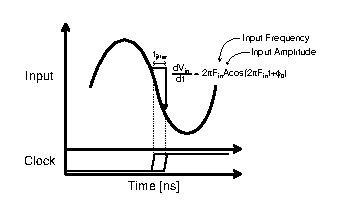
\includegraphics[width=\textwidth]{Chapter5/Figs/lvds/aperture_jitter.ps}
        \subcaption{Aperture jitter representation}
        \label{}
    \end{subfigure}
    \begin{subfigure}[b]{0.48\textwidth}
        \begin{align}
            SNR_{rms}  &= 20\log_{10}\left(\frac{1}{2\pi F_{in}t_{jitter}} \right) \\
            ENOB_{max} &= \frac{SNR-1.76}{6.02}
        \end{align}
        \vspace{2em}
        \subcaption{SNR limit}
    \end{subfigure}
    \caption{Limitation of the SNR and ENOB owing to the variation of the clock period}
    \label{fig:adc-jitter}
\end{figure}

In recent years low-voltage differential signaling (LVDS) has found broad application in consumer electronics, high-speed computer peripherals, telecom/networking, and wireless base stations. LVDS has distinct advantages in performance, power, noise, EMI reduction, and cost. At a rate of 100MHz to 800MHz the LVDS signal can reach as far as 10m to 15m in a twisted-pair cable link, or > 1m in a PCB trace pair. In addition, the power consumption is relatively frequency independent, while the power dissipated in 100$\Omega$ load at the input is often around 1.2 mW in a commercial chip. Usually used in time-sensitive applications and possibly long PCB trace, the LVDS is well suited for the transmission of the clock of high-speed or medium-speed and high-resolution ADCs. The power budget for the LVDS receiver is then fixed to 1.4 mW to allow a margin for an operation at high temperature.

Based on the IEEE 1596 standard for the LVDS, the input differential voltage is in the range of 100 mV to 350 mV as the current of the H-bridge is supposed to be in the range of 1 mA to 3.5 mA and the termination load is 100$\Omega$. In order to select an accurate 100$\Omega$ resistance which does not vary much over temperature, it has been decided to externalize it off-chip. In order to decrease jitter, the design considers the minimization of the intrinsic noise as fundamental as the noise is integrated on the capacitive load of the receiver and the duty cycle shall be preserved.

\begin{figure}[htp]
    \centering
    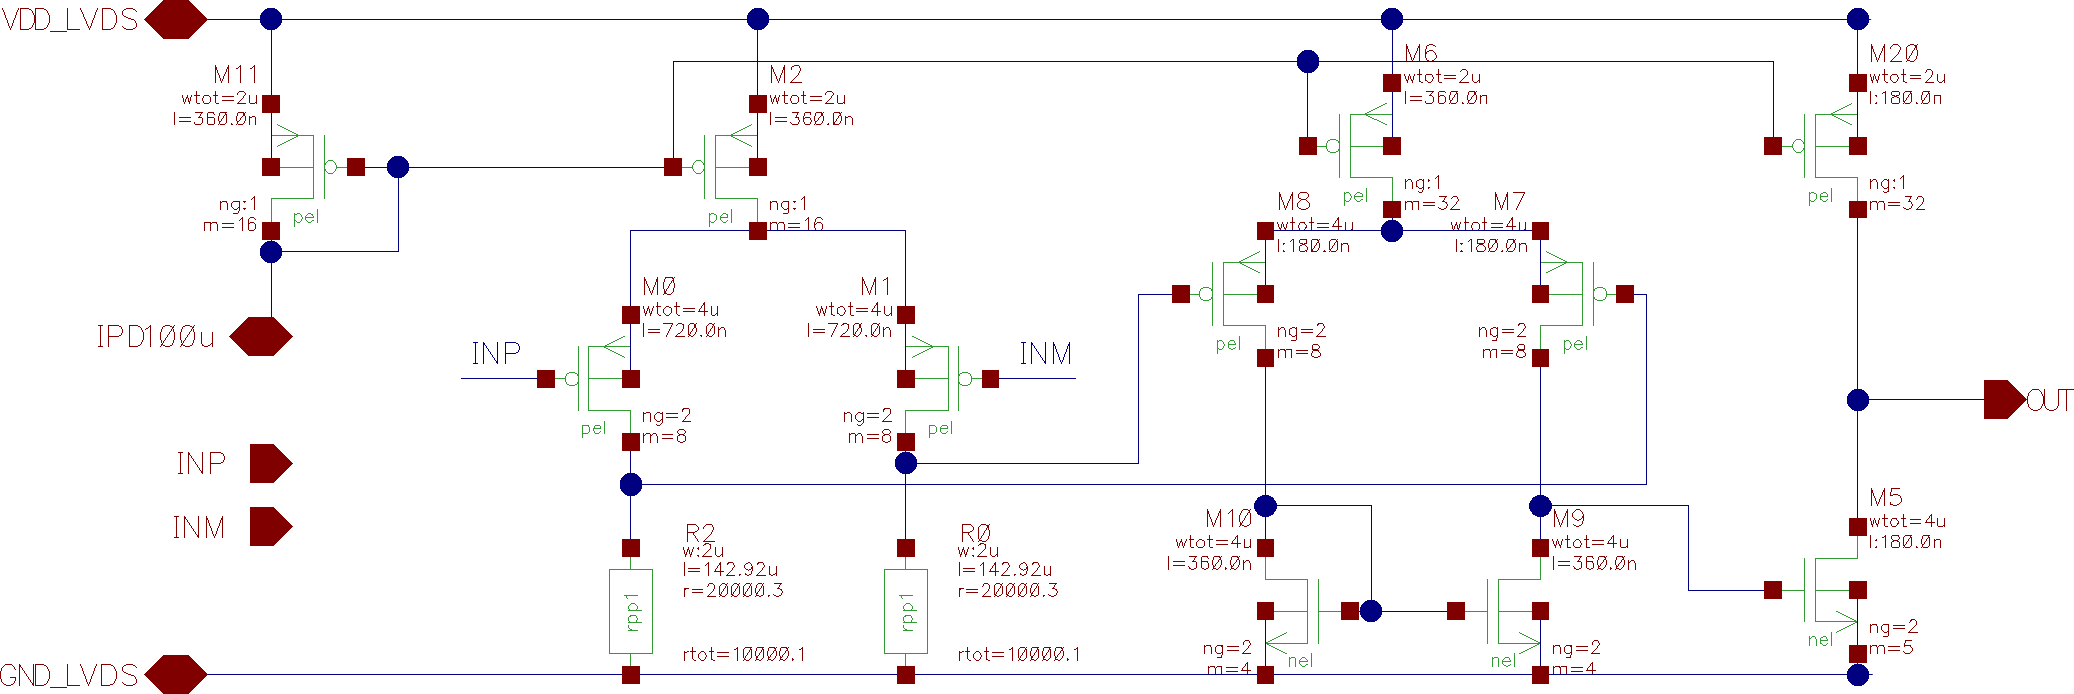
\includegraphics[width=0.9\textwidth]{Chapter5/Figs/adc_chip/clk-recovery.png}
    \caption{LVDS clock receiver to designed for high temperature}
    \label{fig:lvds-receiver}
\end{figure}

According to the section~\ref{sec:analog-insight}, the noise, and the temperature frequency sensitivity are minimized for transistors in moderate or in the weak inversion region. To the contrary, to reduce transition time variations, transistors should operate in strong inversion. Therefore, a multi-stage topology has been selected to blend performances, \figurename~\ref{fig:lvds-receiver}. The first stage is a medium-gain amplifier to minimize the noise figure with $L=4L_{min}$ to reduce the temperature sensitivity. The second stage further amplifies the difference with transistors in strong inversion and with a low gain and reduced parasitic capacitance of differential pair transistors to decrease the accumulated noise of the first stage. Then, the last stage is low-impedance and provides a large current to drive a capacitive load of 100 fF with steep transitions of 250 ps. The noise mostly defined by the first stage and the transition can then be adjusted by a single biasing current IPD100U. By default, the value of the biasing current is 100 $\mu$A based on the period jitter variation.

\begin{figure}[htp]
    \centering
    \begin{subfigure}[b]{0.32\textwidth}
        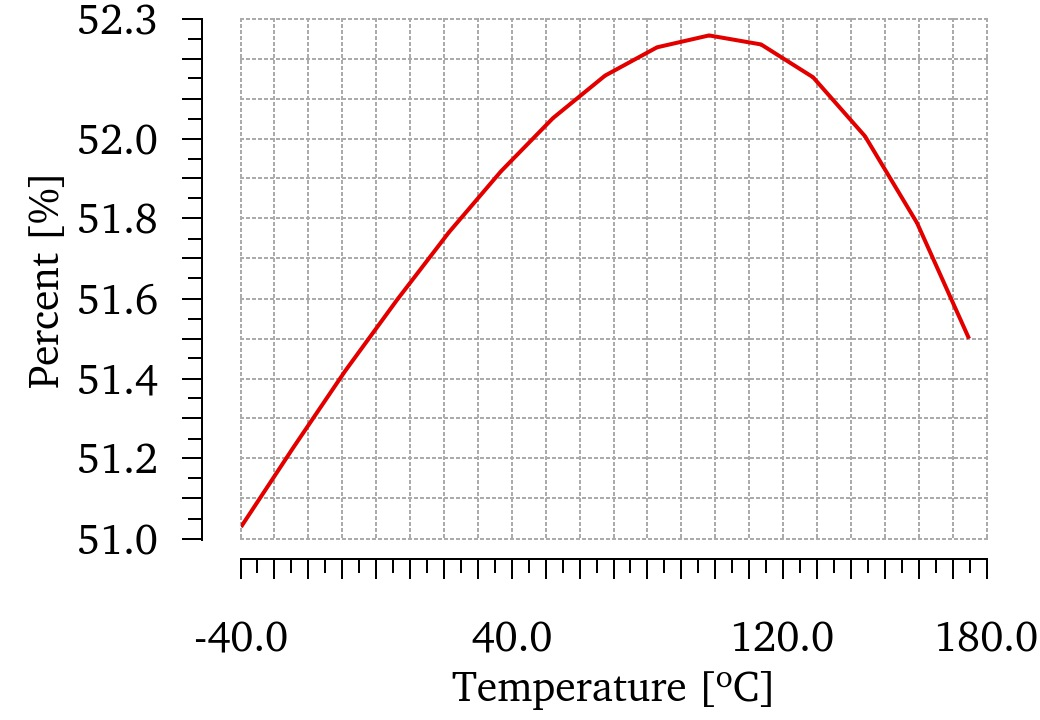
\includegraphics[width=0.9\textwidth]{Chapter5/Figs/lvds/duty_cycle_vcm0_4V.jpg}
        \subcaption{Duty Cycle}
    \end{subfigure}
    \begin{subfigure}[b]{0.32\textwidth}
        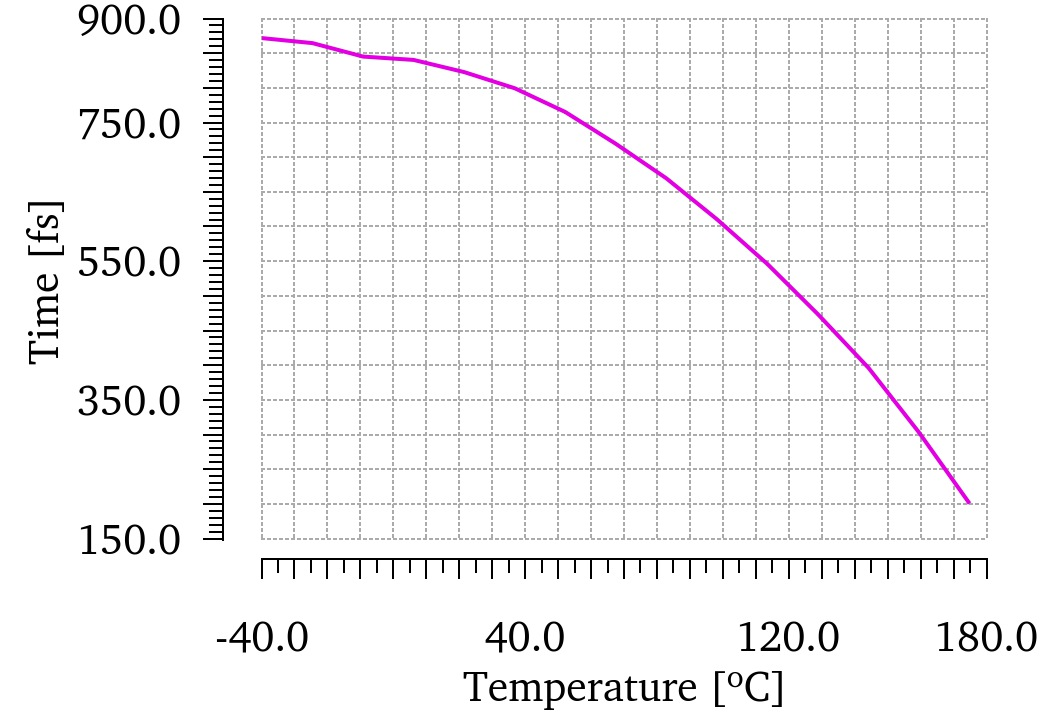
\includegraphics[width=0.9\textwidth]{Chapter5/Figs/lvds/period_jitter_vcm0_4V.jpg}
        \subcaption{Period Jitter}
    \end{subfigure}
    \begin{subfigure}[b]{0.32\textwidth}
        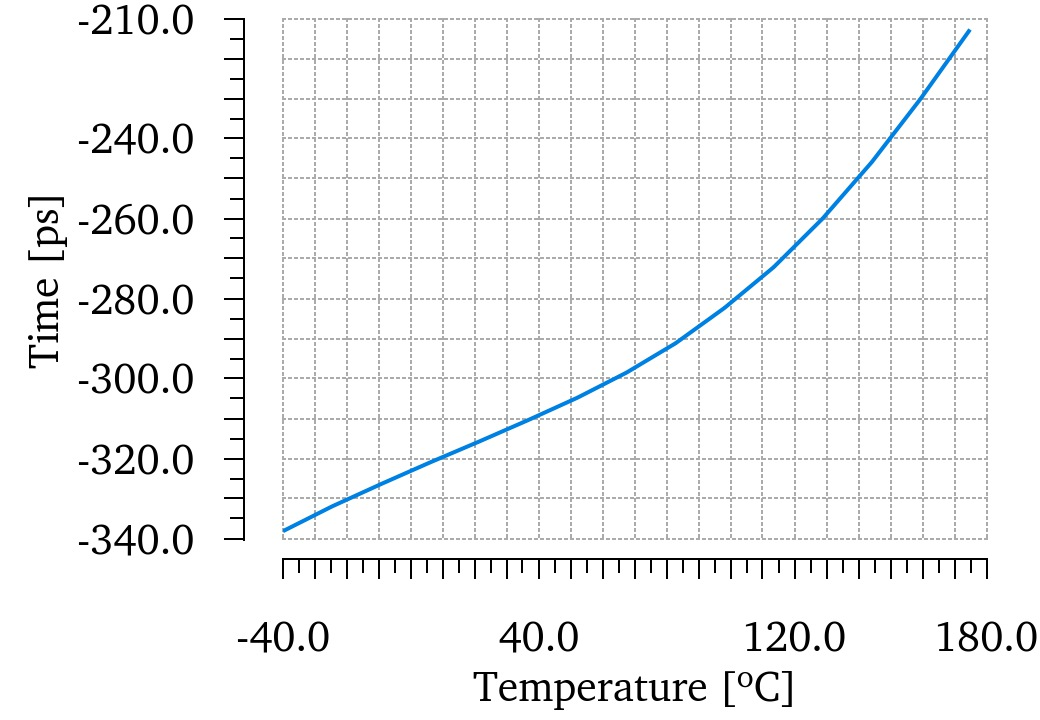
\includegraphics[width=0.9\textwidth]{Chapter5/Figs/lvds/period_error_vcm0_4V.jpg}
        \subcaption{Deterministic Period Error}
    \end{subfigure}
    \caption{LVDS receiver duty cycle and jitter over temperature for $V_{cm} = 400 mV$}
    \label{fig:lvds-receiver-res}
\end{figure}

Simulation results depicted by \figurename~\ref{fig:lvds-receiver-res}, represents the variation due to the temperature and the process variations. The process variations consider the transistor and the resistance alteration while driving a 100 fF capacitive load for a differential input of 100 mV: the minimum detectable voltage of an LVDS signal for a common mode voltage of 400 mV. The period jitter is degraded at low-temperature due to the output common mode voltage of the first stage increasing. In the worst-speed corner, the capacitive load is increased to 110 fF and the resistance is increased by 10\%. Over the manufacturing process variations, ensuring the correct operation over a large common-mode range becomes difficult. Due to this, the capacitive load is reduced to 60 fF to work over a large variation of the common-mode. Otherwise, this solution is able to drive a large capacitive load over the temperature range if the common mode voltage at the input of the receiver is closer from the ideal range as depicted by \figurename~\ref{fig:lvds-receiver-res1V} for $V_{cm} = 1 V$.

\begin{figure}[htp]
    \centering
    \begin{subfigure}[b]{0.32\textwidth}
        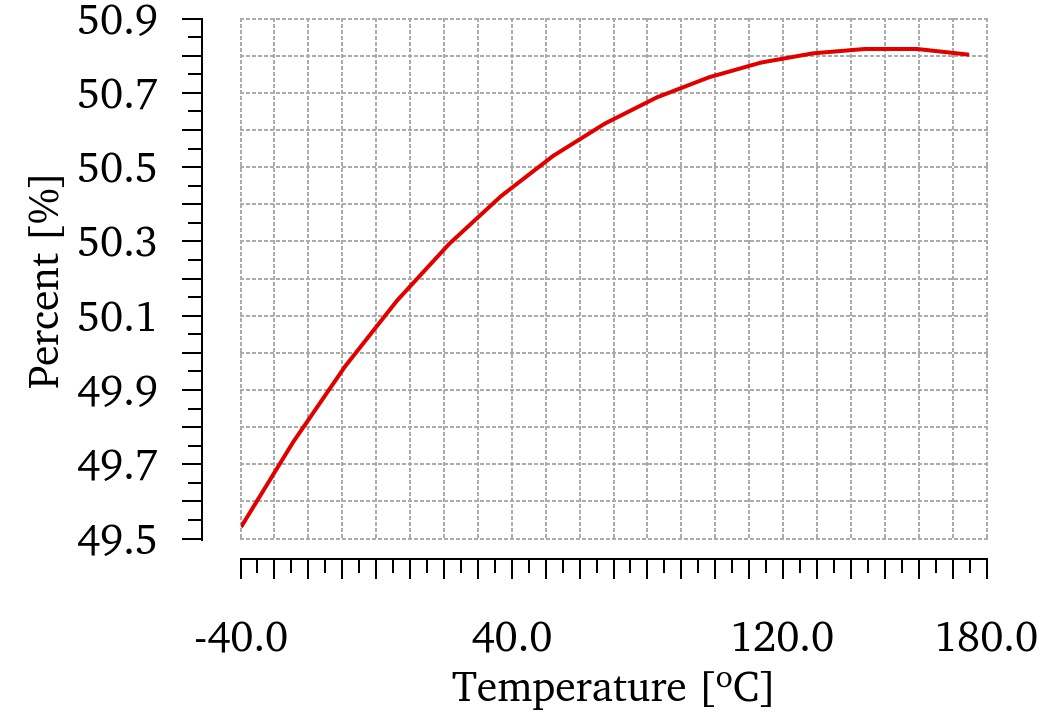
\includegraphics[width=0.9\textwidth]{Chapter5/Figs/lvds/duty_cycle_vcm1V.jpg}
        \subcaption{Duty Cycle}
    \end{subfigure}
    \begin{subfigure}[b]{0.32\textwidth}
        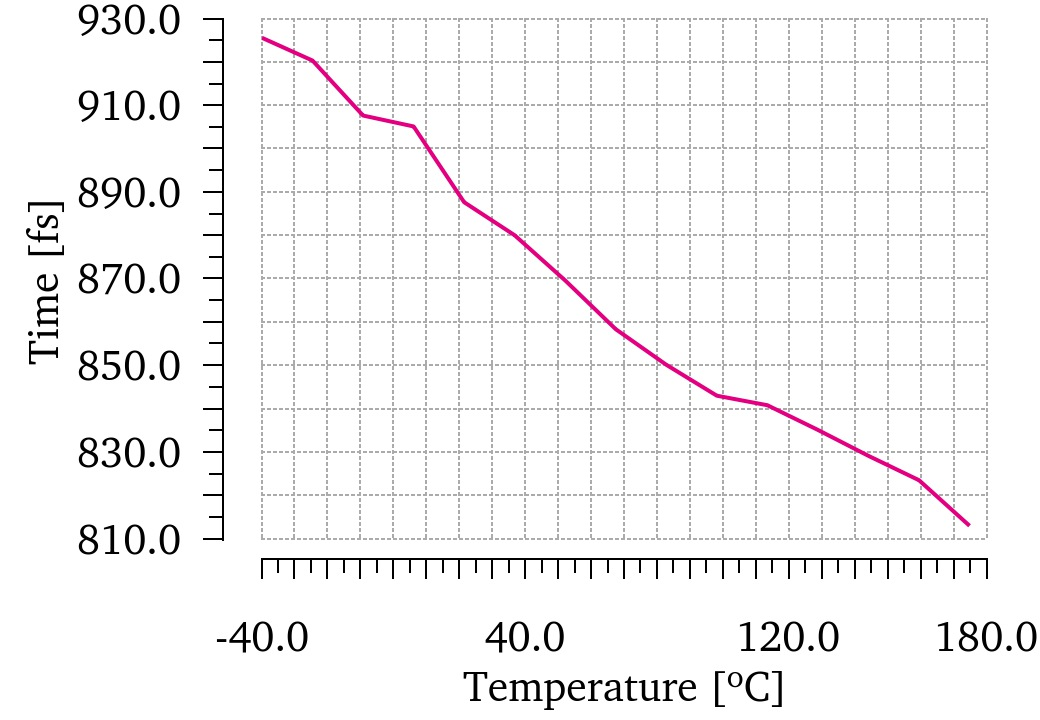
\includegraphics[width=0.9\textwidth]{Chapter5/Figs/lvds/period_jitter_vcm1V.jpg}
        \subcaption{Period Jitter}
    \end{subfigure}
    \begin{subfigure}[b]{0.32\textwidth}
        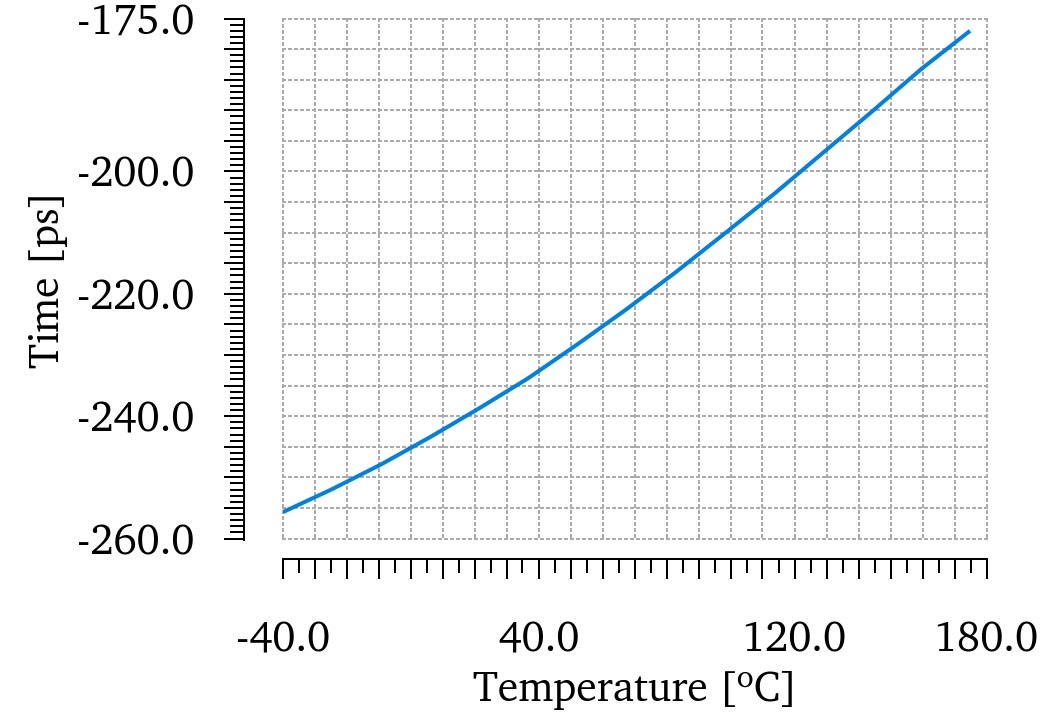
\includegraphics[width=0.9\textwidth]{Chapter5/Figs/lvds/period_error_vcm1V.jpg}
        \subcaption{Deterministic Period Error}
    \end{subfigure}
    \caption{LVDS receiver duty cycle and jitter over temperature for $V_{cm} = 1 V$}
    \label{fig:lvds-receiver-res1V}
\end{figure}

Being sensitive to the input common mode voltage, most LVDS receivers require internal or external fail-safe circuitry so that under a specific link condition or failure the receiver's output will have a known logic condition, usually logic-high. This includes inputs that are either open, floating or shorted.

In favor of a fully integrated LVDS receiver, the fail-safe circuit is also inside the IC\@. The easiest realization of such circuit consists in biasing the 100$\Omega$ load by connecting it to supply via resistors. As represented in the \figurename~\ref{fig:in-path-fail-safe}, this fail-safe function is a simple circuit consisting of three resistors connected externally to the receiver input pins such that the current through the 100$\Omega$ regenerates a sufficient voltage across it to set the CLK signal to 1. $R_1+R_2+R_3$ set the current through $R_2$ which define the differential voltage while $R_3$ set the common mode voltage. This approach operates when the inputs are floating. Unfortunately, this circuit introduces an internal offset in a normal condition which is unbalanced -- degrading the duty cycle and increasing the jitter --. In addition to that, resistors inject power supply noise and thermal noise in the signal path.

\begin{figure}[htp]
    \centering
    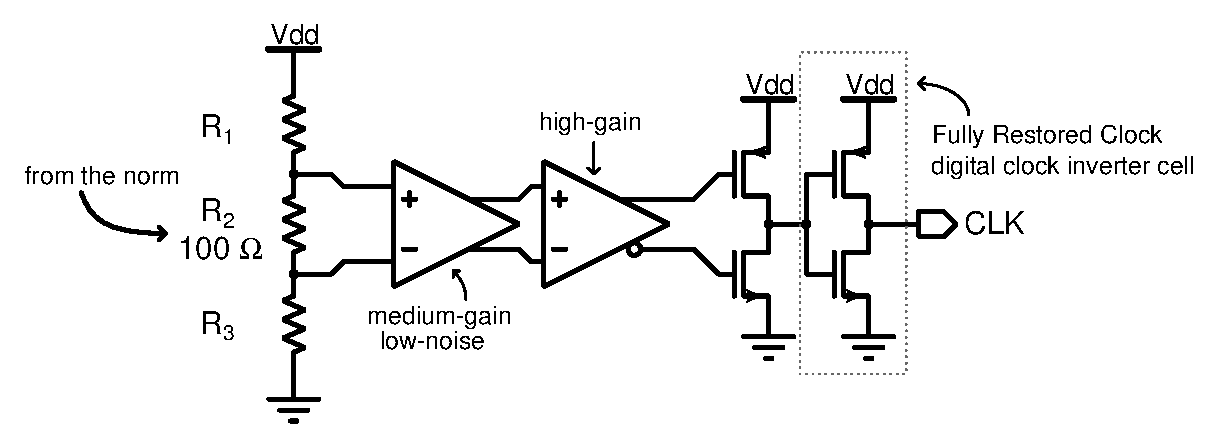
\includegraphics[width=\textwidth]{Chapter5/Figs/adc_chip/lvds-external-failsafe.ps}
    \caption{In-path fail-safe circuit by the biasing with resistor R1 and R3}
    \label{fig:in-path-fail-safe}
\end{figure}


The in-path fail-safe design is similar to the external-biasing fail-safe approach, except that here R1 and R2 are integrated into LVDS receivers so the offset on VID is now a built-in voltage source. This circuit has been used extensively in some LVDS receivers~\cite{TI-SLLA082B}.

To overcome major drawbacks of the prior fail-safe circuit, the failure detection can be in parallel with the signal path. As illustrated in \figurename~\ref{fig:parallel-fail-safe}, this circuit is used in commercial LVDS receivers as in MAX9157 from Maxim Integrated. As shown in this figure, The common mode voltage is compared to a reference voltage $V_{ref}$ usually taken as a $V_{DD}-V_{th}$. In case the inputs are opened or floating, the current injected by the resistor $R_1$ rises the common mode voltage. The voltage ramps up at rate defined by $(R_1+R_3)(C_{pad}+C_{parasitic})$.

\begin{figure}[htp]
    \centering
    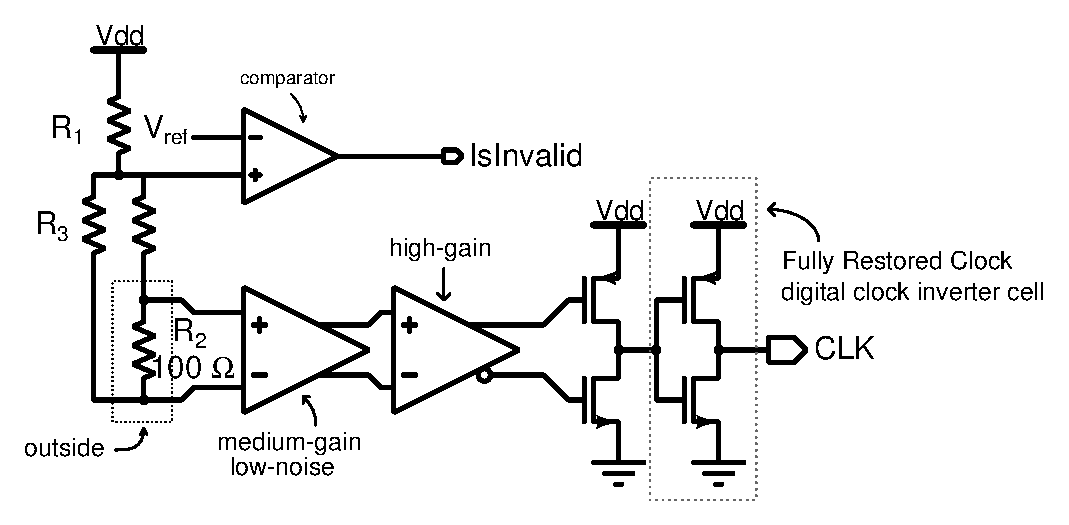
\includegraphics[width=0.8\textwidth]{Chapter5/Figs/adc_chip/lvds-parallel-failsafe.ps}
    \caption{Parallel fail-safe circuit implementation}
    \label{fig:parallel-fail-safe}
\end{figure}

If the link voltage level is higher than the reference, its output goes to logic-high. Then, IsInvalid signal could block the receiver's output through an OR gate and the fail-safe function is activated. This functional design can work properly as long as the common-mode voltage is less than the reference voltage. So, PMOS transistors are preferred to not add an extra common mode voltage limit. Moreover, the parallel-fashion circuit has a much higher noise margin for both the common and differential modes without degradation on the duty cycle and jitter of the input differential signal.

The latter has been designed and sized for a maximum $V_{cm}$ of 1.32 V in a typical case, while in the worst speed corner the error is flagged for a common mode voltage of 1.23 V. This process dependence is necessary as the jitter increase as the clock receiver is slower.

\begin{figure}[htp]
    \centering
    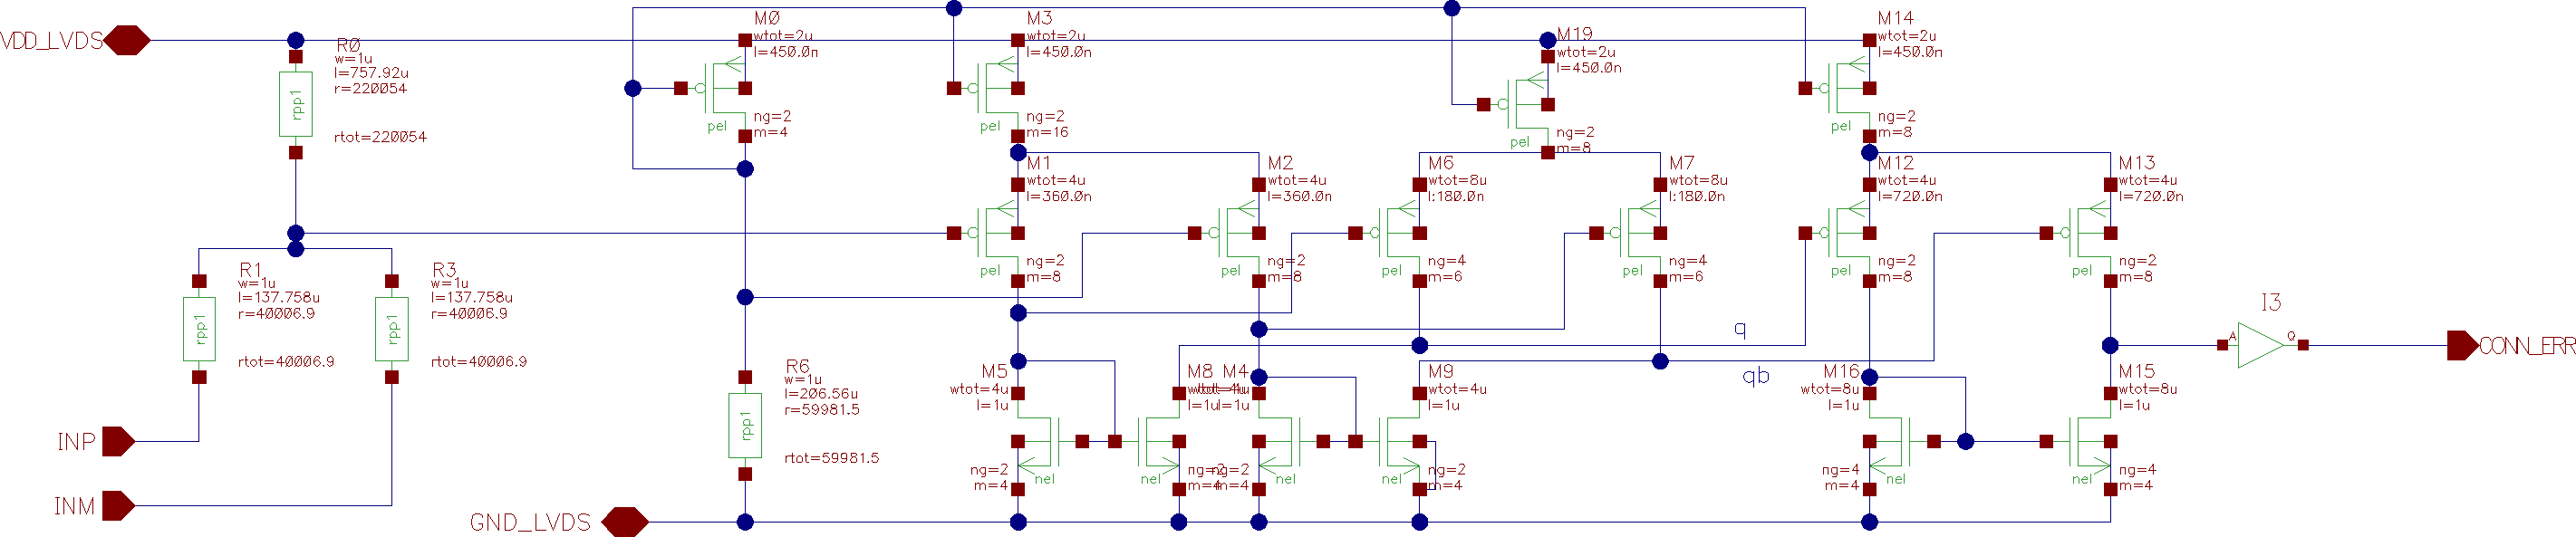
\includegraphics[width=\textwidth]{Chapter5/Figs/adc_chip/lvds-failsafe.png}
    \caption{Schematic of the parallel fail-safe circuit with its biasing circuit}
    \label{}
\end{figure}

With less than 1 ps of period jitter, the proposed LVDS receiver design allows reaching an SNR of 84 dB. This corresponds to an ENOB of 13.6 bits over the full temperature range. In addition to that, the duty cycle at the output of the receiver corresponds to the duty cycle of the input clock with a maximum error of 1.1\%. Thus, the LVDS receiver could be used without causing damage in a conversion at 5 clock cycles per sample. At 6 clock cycles per sample, the period jitter is close to the maximum ENOB of the ideal ADC\@.

In this chapter, we discussed the design of analog building blocks of the ADC\@: the comparators, the OTA, and the LVDS receiver. After a temperature-aware analysis of both a Strong-Arm and a Double-Tail comparator, their design tries to reduce their temperature variation of both the speed and the offset. Post-layout simulation results encourage the use of Strong-Arm comparators for low-power application, and Double-Tail comparators for fully differential application sensitive to the differential kickback. The latter is well suited for charge-redistribution SAR ADCs, while the Strong-Arm comparator found application in the two first stages of the ADC\@.
Concerning the design of the OTA, a gain boosting complementary folded cascode has been selected for its wide-swing, and the slew rate capability of class-AB amplifiers. Its design has been focused on the reduction of the settling error under PVT variations, and the noise reduction afterward. Despite a large DC Gain variation over temperature, the limiting factor to reach small settling errors is mainly the speed of the OTA\@.
Finally, we designed an LVDS receiver for the specific needs of the ADC\@. A careful attention is paid to the period jitter limiting the maximum ENOB achievable.
However, this chapter only presents simulation and post-layout simulation results. This is not sufficient to reuse them as validated IP blocks.
